
\section{The angle of Incidences influence on the headphone transfer function} \label{sec:AngleOfIncidence}

All data from this experiment can be found at
 \path{CD:\\Appendices\Appendix H - The Angles of Incidences Influence on the Headphone Transfer-Function\..}

\subsection{Purpose}
The purpose of this experiment is to determine if the angle of incidence has any influence on the headphone transfer function. 

The hypothesis is that the angle on incidence influences both the time delay and magnitude response of the transfer functions. Measurements will only be performed in a horizontal plane. 

\subsection{AAU num list}

Table \ref{tab:AngleOfIncideceHP} list the equipment used during the experiment.

\begin{table}[H]
	\centering
	\ra{1.3}
	\begin{tabular}{ c c c } \toprule
		{Item}	& {Description} 						& {AAU-no}. \\ \bottomrule 
		1	&	B\&K Head And Torso Simulator "Henry" Type 4128	& 08453	\\
		2	&	B\&K ½'' Condenser Microphone Type 4134 	& 08130		\\
		3	&	Beyerdynamic DT 770 Headphones				& 2037-18		\\
		4	&	Soundcard RME Fireface 802					& 86838		\\
		5	&	Computer running simulink		& NaN		\\
		6	&	GRAS pre-amplifier type 26-AK			& 52665		\\
		7	&	B\&K Sound Calibrator Type 4230				& 08155		\\ 
		8	&	Knowles FG-23329 microphone					& NaN		\\
		9	&	Genelec speaker								& 33990		\\ 
		10	&	Preamp for FG-23329  microphone	& NaN\\
		11	& 	B\&K Microphone Power Supply Type 2804		& 07304		\\
		\bottomrule
	\end{tabular}
	\caption{Table over equipment used during the experiment.}
	\label{tab:AngleOfIncideceHP}
\end{table}

\subsection{Diagram}

Figure \ref{fig:AngleOfIndDiagram} shows the idea assumed behind the experiment. By rotating the head, it is possible to determine the difference in time between the Speaker microphone and Reference microphone. The calculation is done based upon figure \ref{Fig:AngleOfIcidenceTriangleCalculation} and is further described in section \ref{sec:AngleDescription}.

\begin{figure}[H]
	\centering
	\begin{subfigure}[b]{.4\textwidth}
		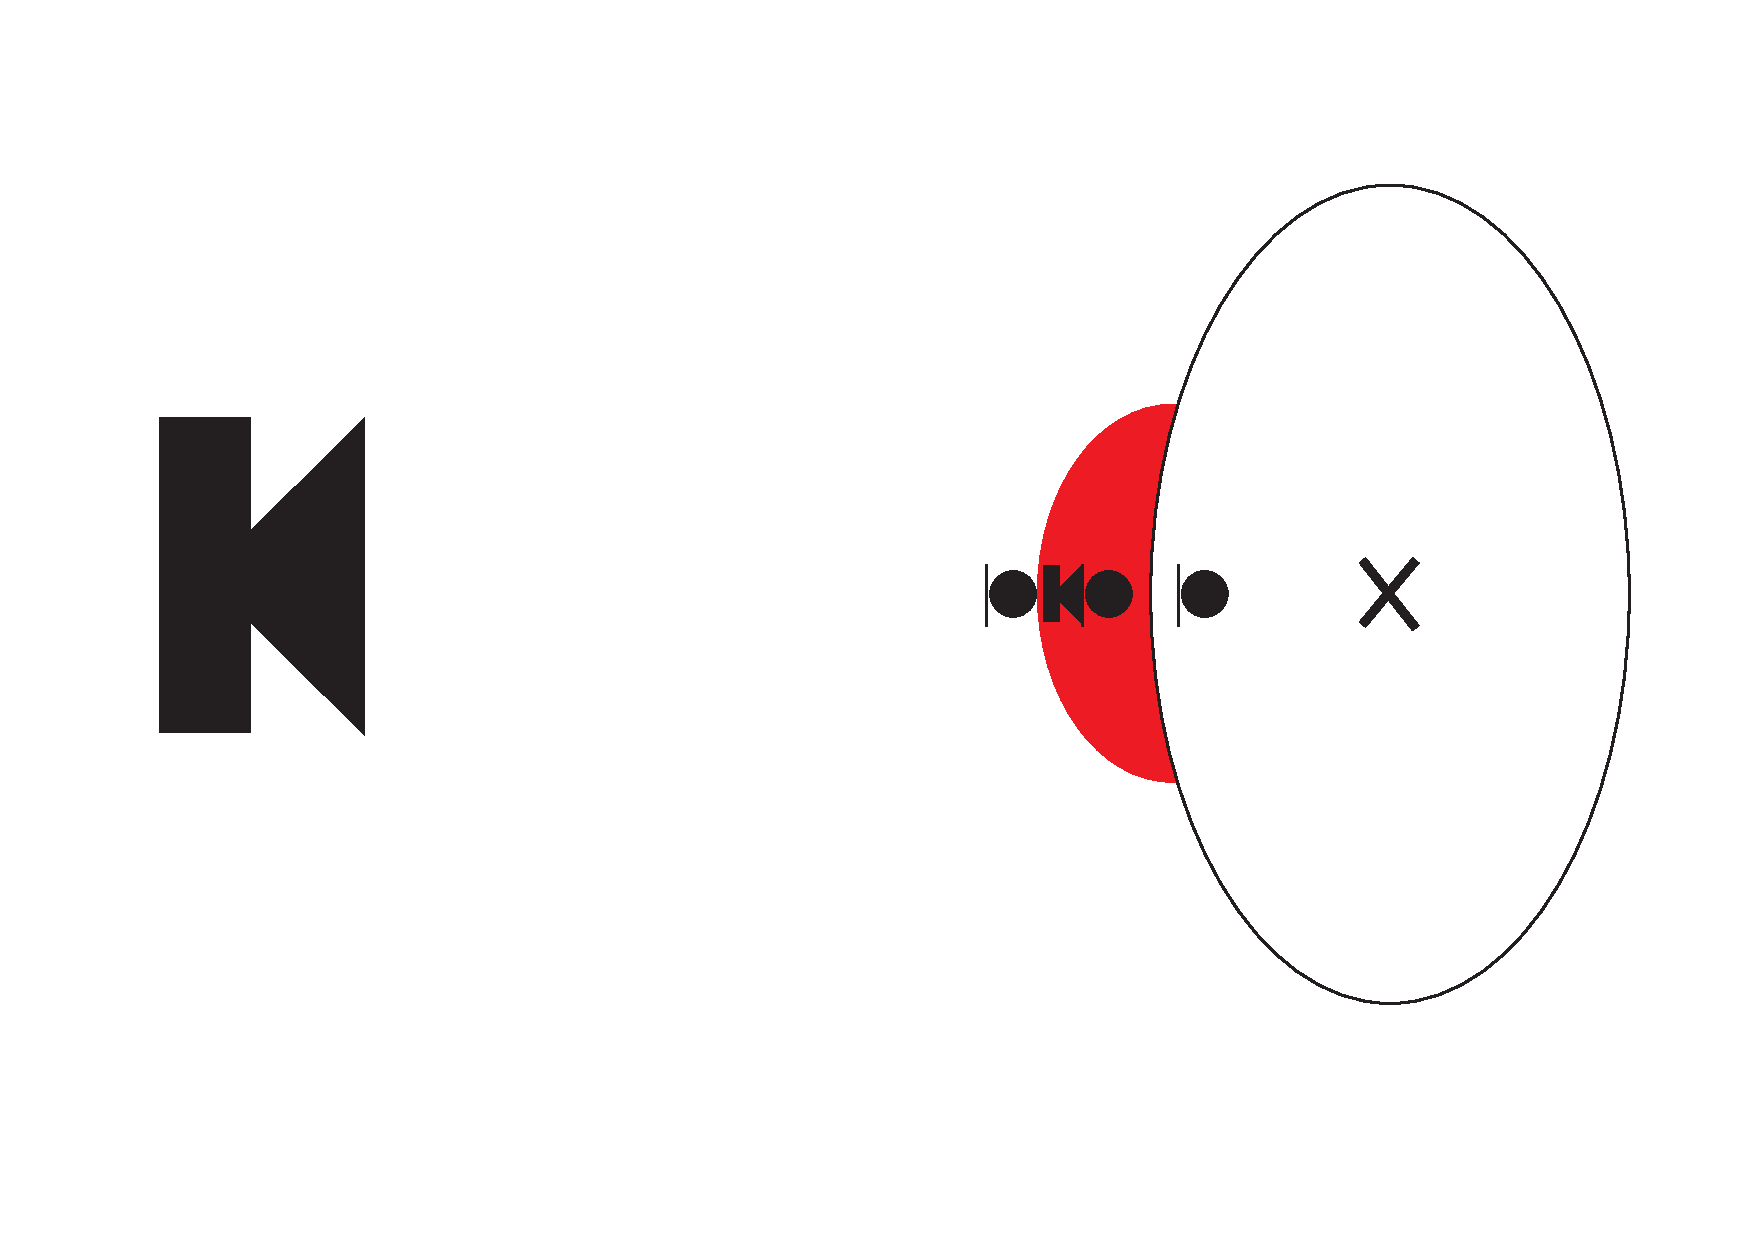
\includegraphics[width=\textwidth]{../Journal/Experiments/AngleOfIncidence/AngleOfIncidenceOnAxis.pdf}
		\caption{On axis}
		\label{fig:AngOfIndOnax}
		\vspace{2ex}
		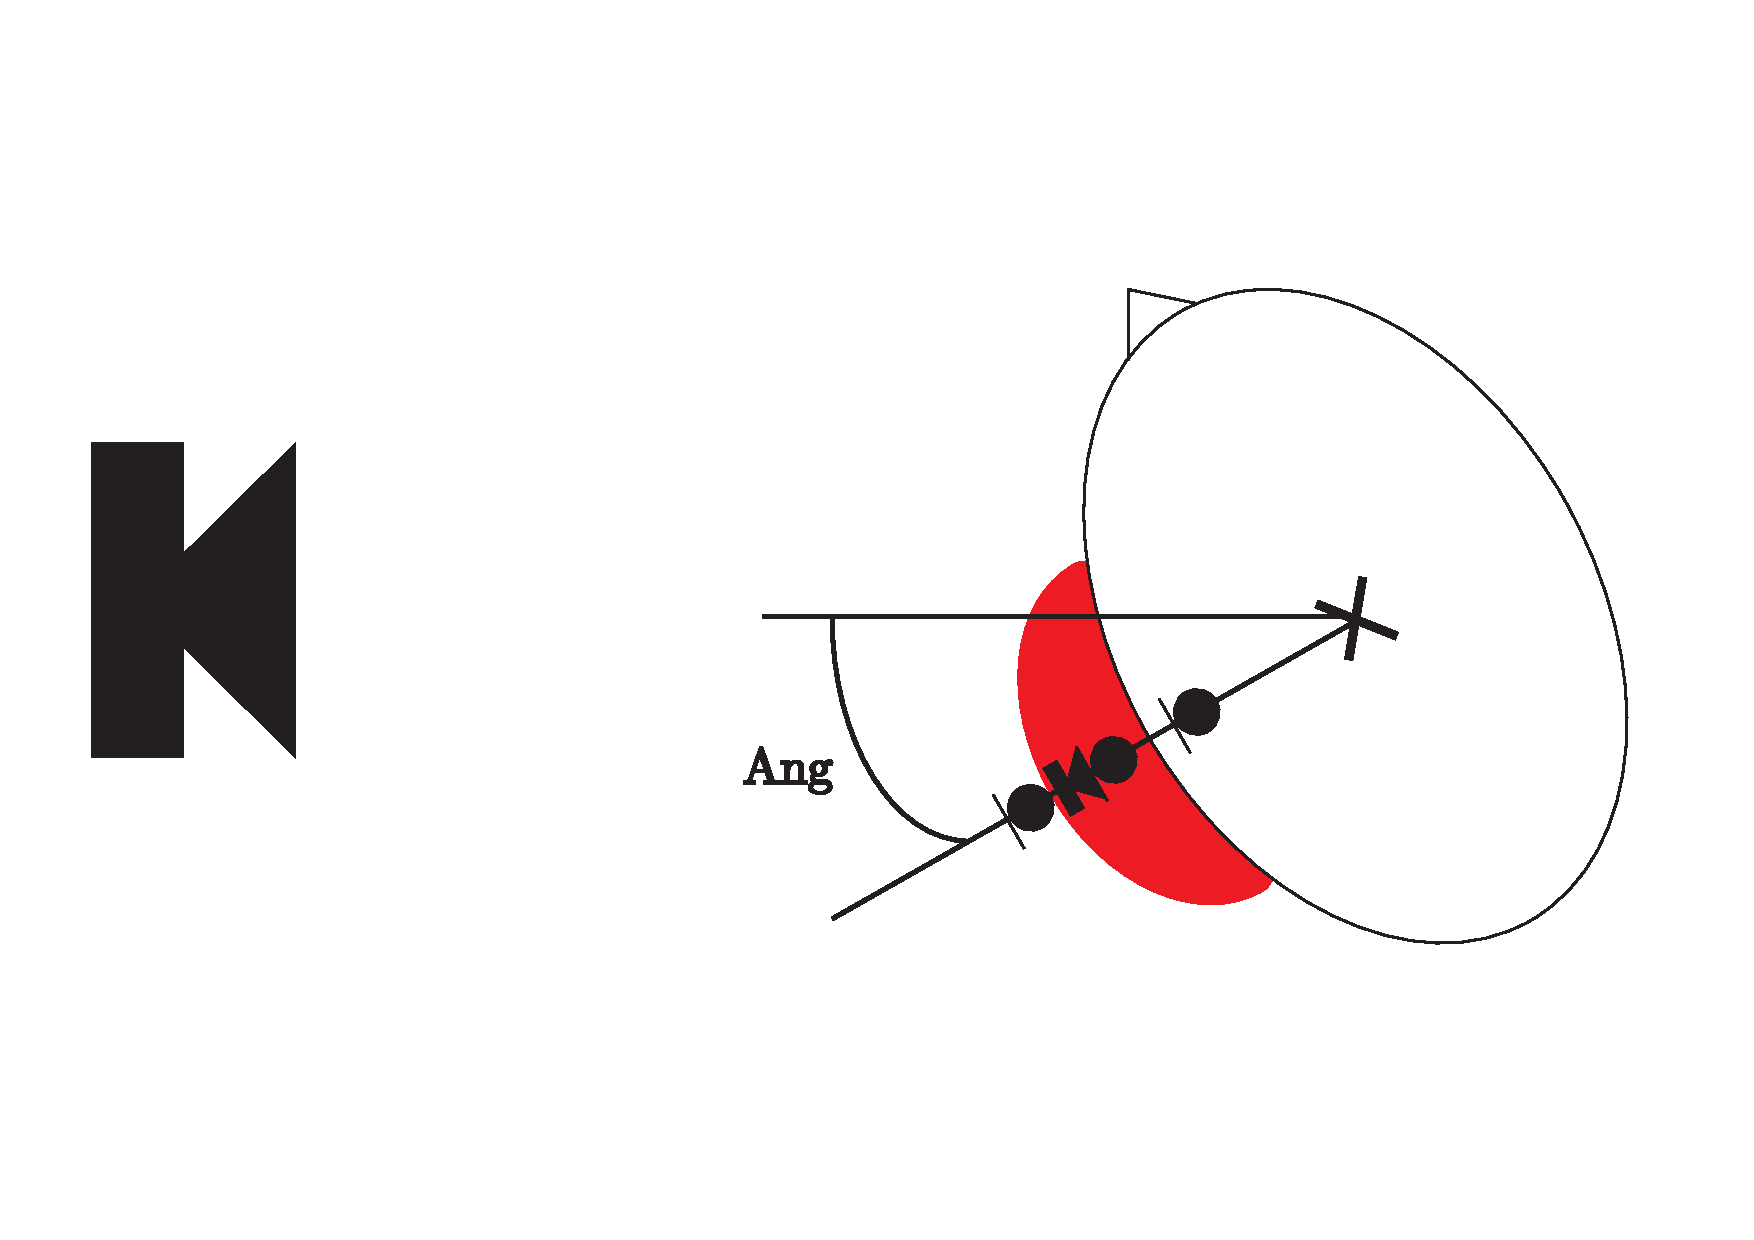
\includegraphics[width=\textwidth]{../Journal/Experiments/AngleOfIncidence/AngleOfIncidenceOffAxis.pdf}
		\caption{Off axis}
		\label{fig:AngOfIndOffax}
	\end{subfigure} 
	\begin{subfigure}[b]{.4\textwidth}
	\centering
	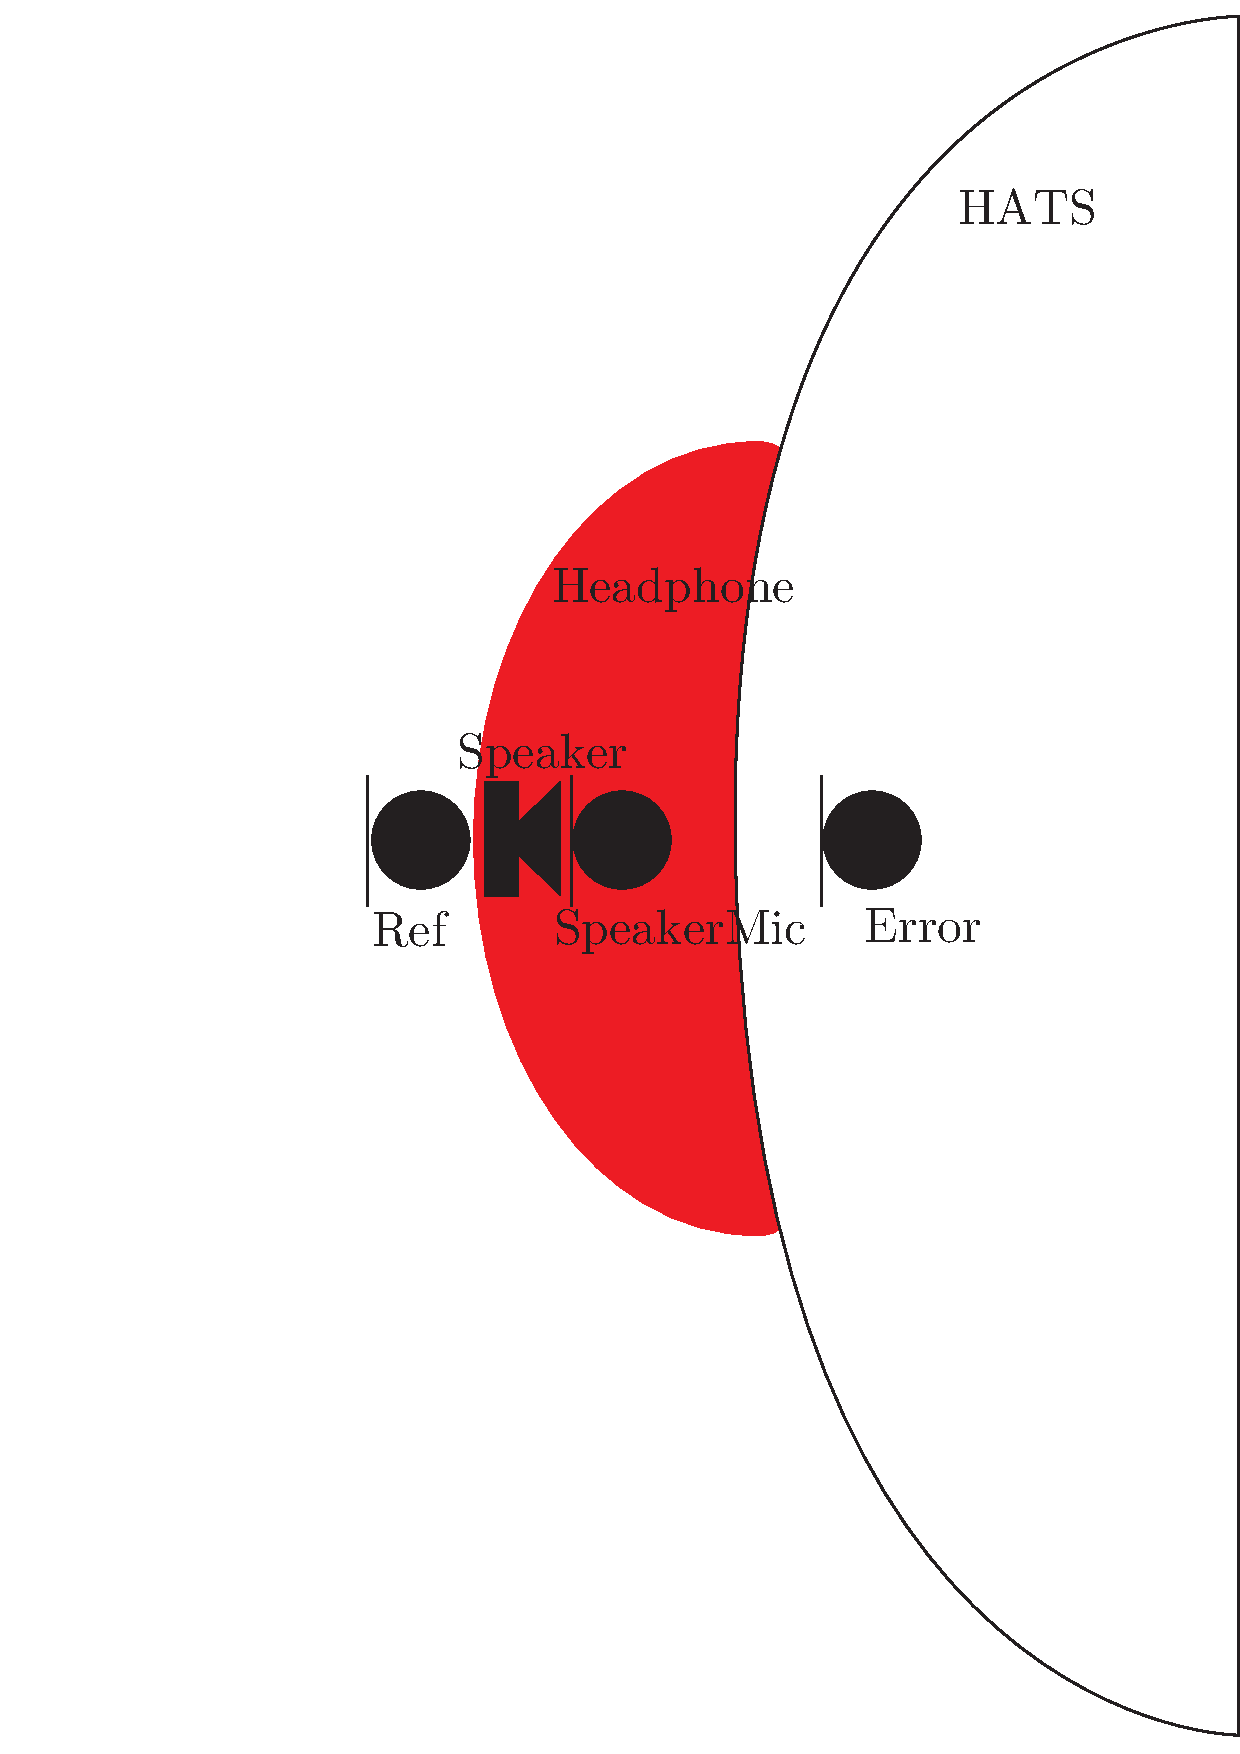
\includegraphics[width=\textwidth]{../Journal/Experiments/AngleOfIncidence/AngleOfIncidenceSchematic.pdf}
	\caption{Placement of microphones.}
	\label{fig:AngOgIndMicplace}
\end{subfigure}
	\caption{Placement of microphones and rotation}
	\label{fig:AngleOfIndDiagram}
\end{figure}


\subsection{Description}\label{sec:AngleDescription}
The experiment uses a single speaker to measure angles of incidence. Therefore either the speaker has to be moved around or the HATS will have to be turned to the right angles. \\
Adjusting the angle is done by rotating the HATS around the centre of the HATS leaving the speaker in place. This creates a triangle between the speaker, microphone and inner microphone of the HATS. The resolution of the scale on the HATS is 2\degrees. The baseline of the triangle is from the microphone to the inner microphone, and angle is adjusted according to that line.
The following angles are examined:
\begin{table}[H]
	\centering
	\begin{tabular}{c c c c c c c c c c} \toprule
		0\degrees & 10\degrees & 20\degrees & 30\degrees & 40\degrees & 50\degrees & 60\degrees & 70\degrees & 80\degrees & 90\degrees \\ \bottomrule
	\end{tabular}
\label{Tab:AngleOfInciMeasAngles}
\caption{Angles that measurements should be performed at. 0\degrees  is the situation in \autoref{fig:AngOfIndOnax}.}
\end{table}
 
% The following Matlab code is used to calculate the angles at which measurements should be performed. The first measurement is performed at a 180\degrees angle. This determines the length of the baseline (maxI in the code below). After determining the angles of interest can be calculated.  \\
%The script is based on two triangles that share a corner, the turning point, and a side to the speaker. The two triangles share the same angle at the turning point. This creates for two equations with two unknowns using the cosine relation and the fact that the side opposite the turning point should have a length "x" in one triangle and "x" + an amount of samples in the other triangle. Using this the angle can  be found.

\begin{figure}[H]
%	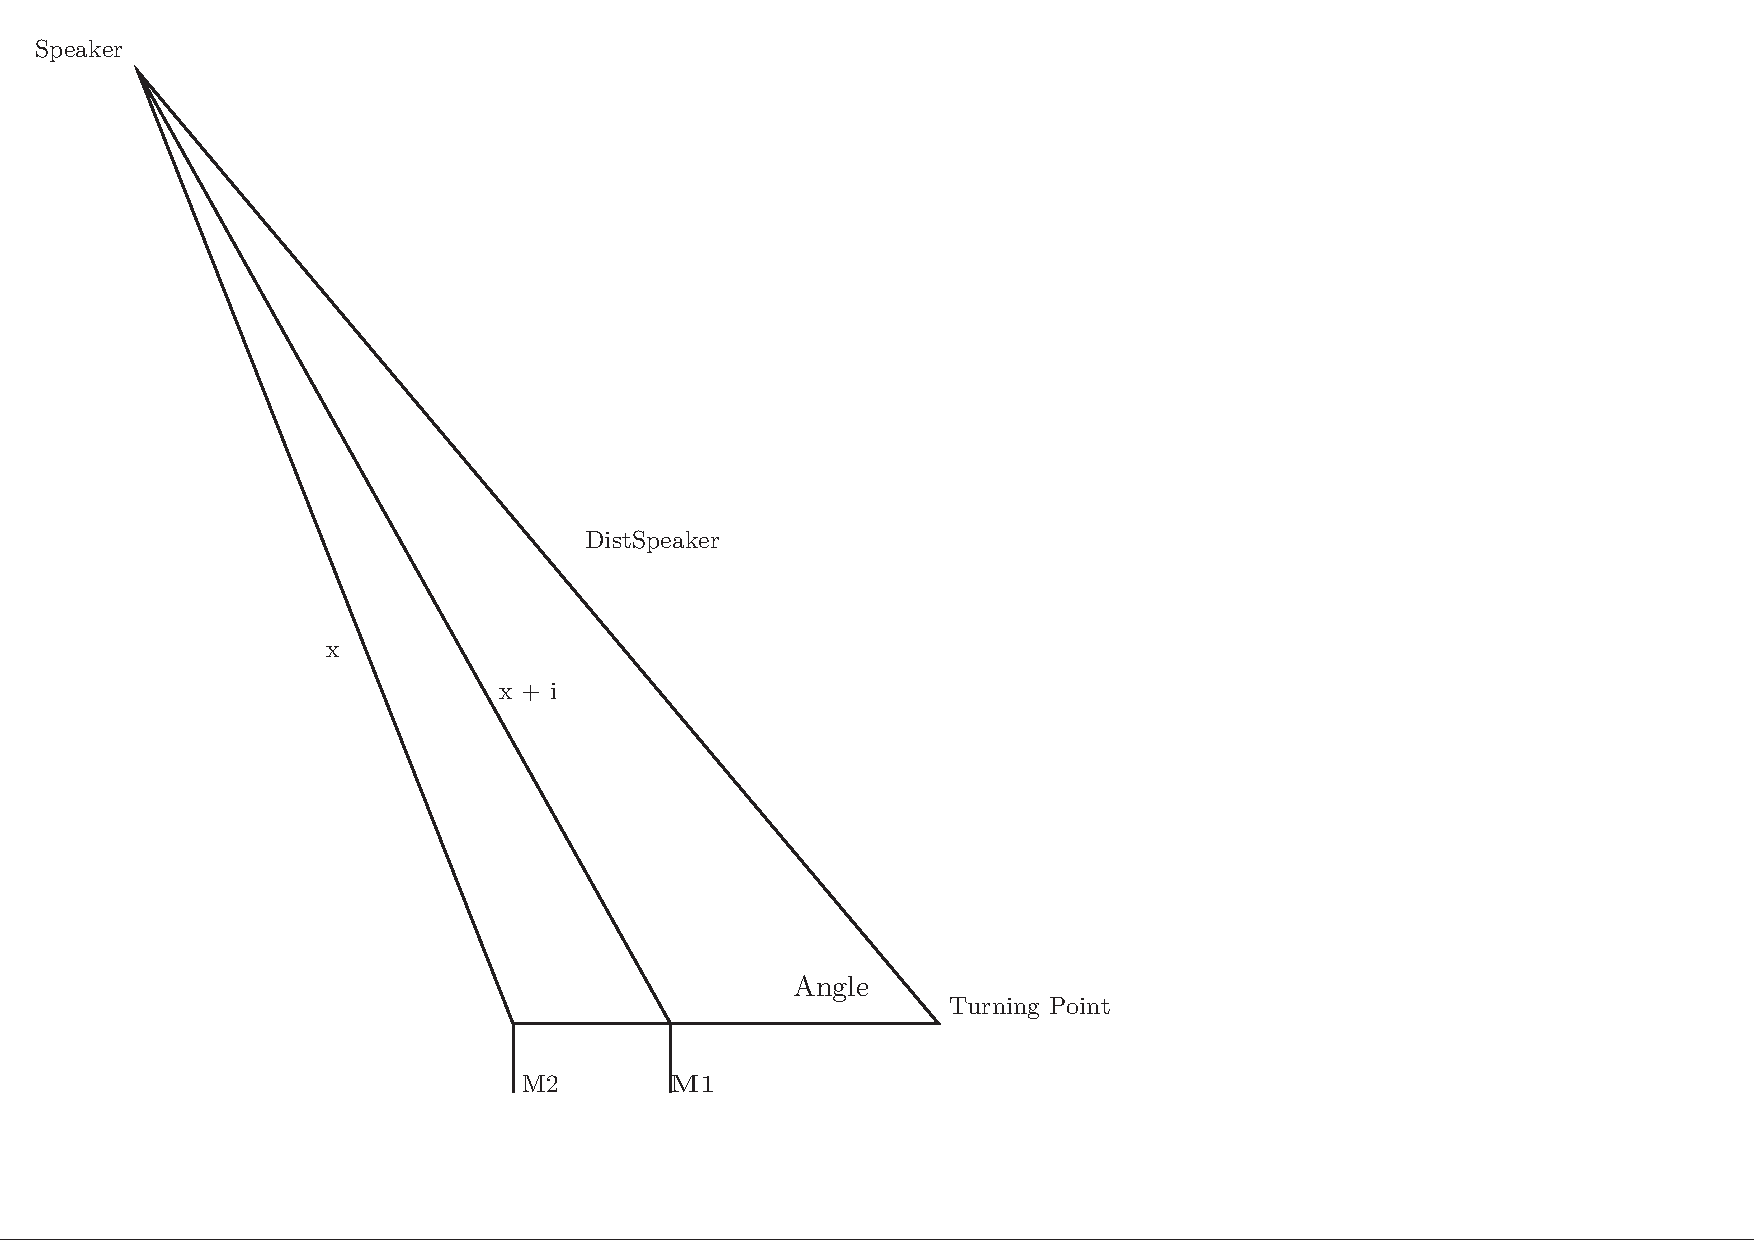
\includegraphics[width=\textwidth]{../Journal/Experiments/AngleOfIncidence/TriangleCalculation.pdf}
\tikzsetnextfilename{AngleOfIcidenceTriangleCalculation}
\begin{tikzpicture}
\draw (4,0) node (v3) {} -- (-1,0);
\draw (-1,0) -- (-3,0);
\draw (-3,0) -- (-3,-0.6);
\draw (-1,0) node (v1) {} -- (-1,-0.6);
\draw (-5,5) node (v2) {} -- (-1,0) -- (-5,5) node (v4) {} -- (-3,0);
\draw (4,0) -- (-5,5);
\node at (-5.1,5.7) {Speaker};
\node at (-3,-0.9) {SpeakerMic};
\node at (-1,-0.9) {Ref};
\node at (5.3,-0.1) {Turning Point};
\node at (2.8,0.2) {Angle};
\node at (0.7,2.5) {$Dist_{Speaker}$};
\node at (-1.9,2) {$x+i$};
\node at (-4.2,2) {$x$};
\end{tikzpicture}
\label{Fig:AngleOfIcidenceTriangleCalculation}
\caption{The two triangles spanned by the center of the HATS, the speaker and two of the microphones.}
\end{figure}  


\subsection{Set-up}

A schematically overview of the experiment is shown in figure \ref{Fig:AngleOfIncidenceSetup}. The experiment is controlled via the RME Fireface 802, which acts as both the recording device and signal generator. A picture of the setup is shown in figure \ref{AngIncidenceSetup}.

\begin{figure}[H]
	\centering
	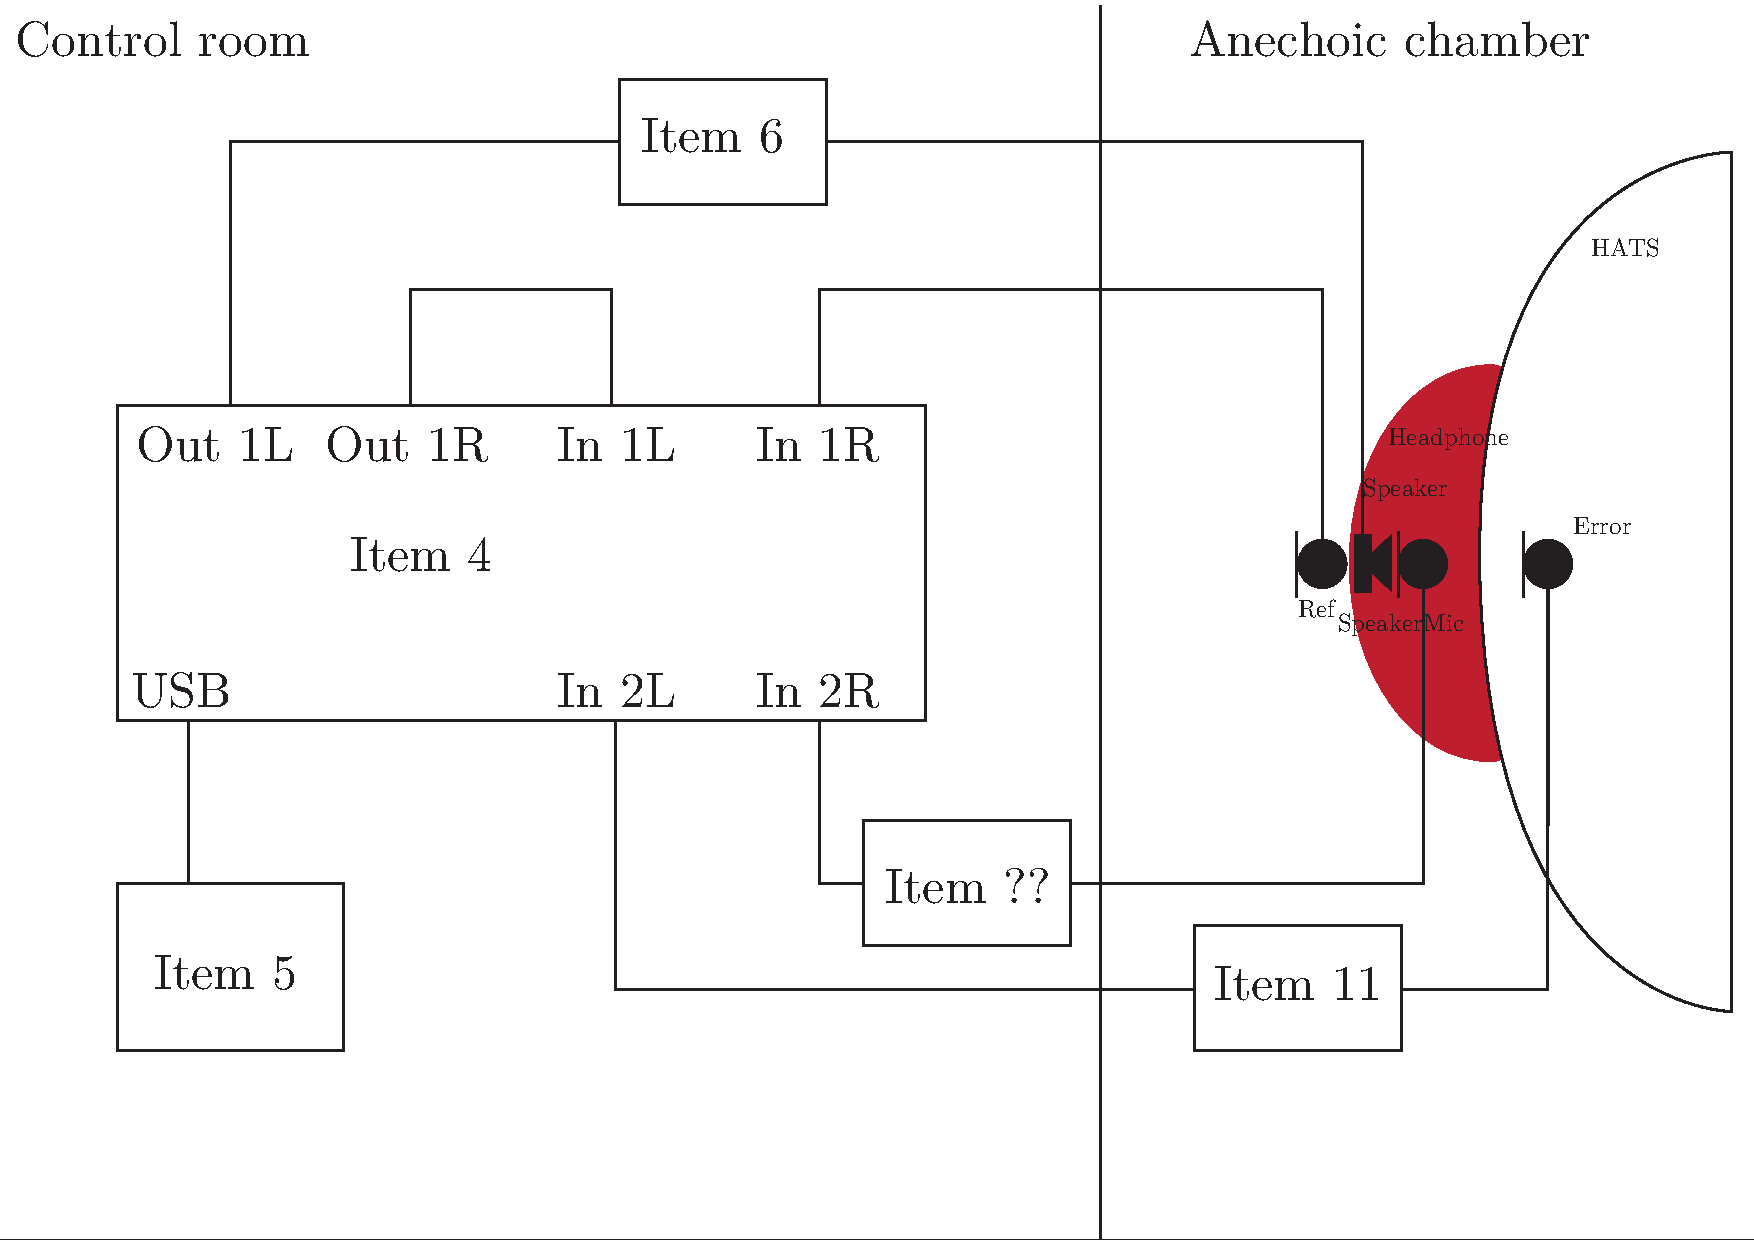
\includegraphics[width=0.75\textwidth]{../Journal/Experiments/AngleOfIncidence/AngleOfIncidenceSetup.pdf}
	\caption{Setup of experiment on angle of incidence.}
	\label{Fig:AngleOfIncidenceSetup}
\end{figure}

\begin{figure}[H]
	\includegraphics[width=\textwidth]{../Journal/Experiments/AngleOfIncidence/AngInSetup.jpg}
	\label{AngIncidenceSetup}	
	\caption{Setup of the experiment.}
\end{figure}

\subsection{Choice of equipment}
The experiment aims to be valid in the frequency range 50Hz to 20 $k$Hz. This means that all equipment used should cover that frequency range. \\\\
The experiment uses a total of three microphones. The error microphone located inside the HATS's ear is given by the type fitted to the dummy. The SpeakerMic should be as small as possible in order to avoid influencing the transfer functions that are being measured. For this a Knowles FG-23329 is used, since this being the smallest readily available. The Ref microphone has less restrictions on size and placement. This allows for the choice of a standard measurement microphone, here the B\&K 4134 is chosen. \\\\
For the speaker, the limiting criteria is the lower roll off, especially in an anechoic chamber were reflections does not offer any amplification of lower frequencies. However transfer functions between the microphones are measured, so absolute flatness is not critical. The Genelec 1031-A is chosen. \\\\
The measurement system uses a RME Fireface 802 controlled using Simulink\textsuperscript{\textregistered}. Data extraction is made using the method described in \autoref{Sec:MeasATransFunc}.

\subsection{Control and calibration}
The speaker is placed 1.6 meters from the center of the HATS. \\\\
The two microphones SpeakerMic and Ref are fixed at distances 8.85 cm and 12.45 cm from the center of the HATS respectively. The SpeakerMic is fitted just in front of the headphone speaker using medical tape.\\\\
For each microphone and pre-amplifier calibrations are made on the computer using Simulink\textsuperscript{\textregistered}.
\begin{itemize}
	\item For the Ref microphone, calibration is made at 1 $k$Hz using the B\&K 4230 as calibrator. This should yield a signal of 93.6 dB as it is a pressure field microphone. The measured intensity in MATLAB\textsuperscript{\textregistered} was 68.99 dB so all measurements are multiplied by 17.00 to get a calibrated signal in MATLAB\textsuperscript{\textregistered}. 
	\item For the Error microphone, calibration is made at 1 $k$Hz using the B\&K 4230 as calibrator with adapter B\&K 0741 for the ear of the HATS. This should yield a signal of 95.6 dB. The measured intensity in MATLAB\textsuperscript{\textregistered} was 78.22 dB so all measurements are multiplied by 7.40 to get a calibrated signal in MATLAB\textsuperscript{\textregistered}. 
	\item For the speakerMic, calibration is made using a earplug cut in half and fitted around the microphone, as an adapter. This simple adapter allows the B\&K 4230 to be used as calibrator. The measured output level is 84.37 dB, and should have been 94.0 dB . Therefore all measurements are multiplied by 3.03 to get a calibrated signal in MATLAB\textsuperscript{\textregistered}
\end{itemize}
 
\subsection{Equipment settings}
\begin{itemize}
	\item This experiment is performed with a sampling rate of, $F_{s}$ = 48 $k$Hz.
	\item The Ref microphone is placed just outside the headset in-line with the ear and speaker unit. 
	\item The SpeakerMic is placed inside the headphone, as close to the speaker unit as possible. 
	\item For on the RME, the "inst"-option is turned on in the mixing console. The following gain settings are present: 		
	\begin{itemize}
		\item Line level gain is 0 dB
		\item Error Microphones has gain +30 dB
		\item Ref Microphones has gain +48 dB
		\item Speaker Microphones has gain +48 dB
	\end{itemize}
	\item All settings on the computer is set to 0 dBFS
	\item A logarithmic sine sweep is generated and saved in MATLAB\textsuperscript{\textregistered} using the chirp function as follows:
	\begin{lstlisting} [language=Matlab	]
	fs=48000;
	f1=50;
	f2=fs/2;
	t=0:1/fs:5-1/fs;
	t2=5;
	sweep=chirp(t,f1,t2,f2,'logarithmic',90);
	sweep=[zeros(1,fs) sweep zeros(1,fs)];
	audiowrite('LogChirp.wav', sweep,fs);
	\end{lstlisting}
\end{itemize}



\subsection{Procedure}
\begin{enumerate}
	\item Set the HATS to the desired test angle. 
	\item Open Simulink\textsuperscript{\textregistered} and run file \path{SimulinkAngleOfIndence.xls}.
	\item Run Simulink\textsuperscript{\textregistered} to play \path{LogChirp.wav} through the speaker.
	\item Record and save, and name \path{Mic[i].wav}, \path{SpM[i].wav}, \path{loop[i].wav} and \path{Ref[i].wav}\footnote{[i] indicates the angle of the experiment}.
	\item Repeat the experiment for all angles.
\end{enumerate}

\subsection{Data Extraction}

All data is automatically stored when the script \path{SimulinkAngleOfIndence.xls} is run.



\subsection{Analysis}
The cross correlation method described in \autoref{Sec:MeasATransFunc} is used to find the transfer functions. The Reference microphone is used as input signal and the speakerMic is used as output. The system under test is the cup of the headphone. 
Below the frequency response and time response of the system is plotted. 
\begin{figure}[H]
	\tikzsetnextfilename{AngOfIncFreq}
	% This file was created by matlab2tikz.
%
%The latest updates can be retrieved from
%  http://www.mathworks.com/matlabcentral/fileexchange/22022-matlab2tikz-matlab2tikz
%where you can also make suggestions and rate matlab2tikz.
%
\definecolor{mycolor1}{rgb}{0.00000,0.44700,0.74100}%
\definecolor{mycolor2}{rgb}{0.85000,0.32500,0.09800}%
\definecolor{mycolor3}{rgb}{0.92900,0.69400,0.12500}%
\definecolor{mycolor4}{rgb}{0.49400,0.18400,0.55600}%
\definecolor{mycolor5}{rgb}{0.46600,0.67400,0.18800}%
\definecolor{mycolor6}{rgb}{0.30100,0.74500,0.93300}%
\definecolor{mycolor7}{rgb}{0.63500,0.07800,0.18400}%
%
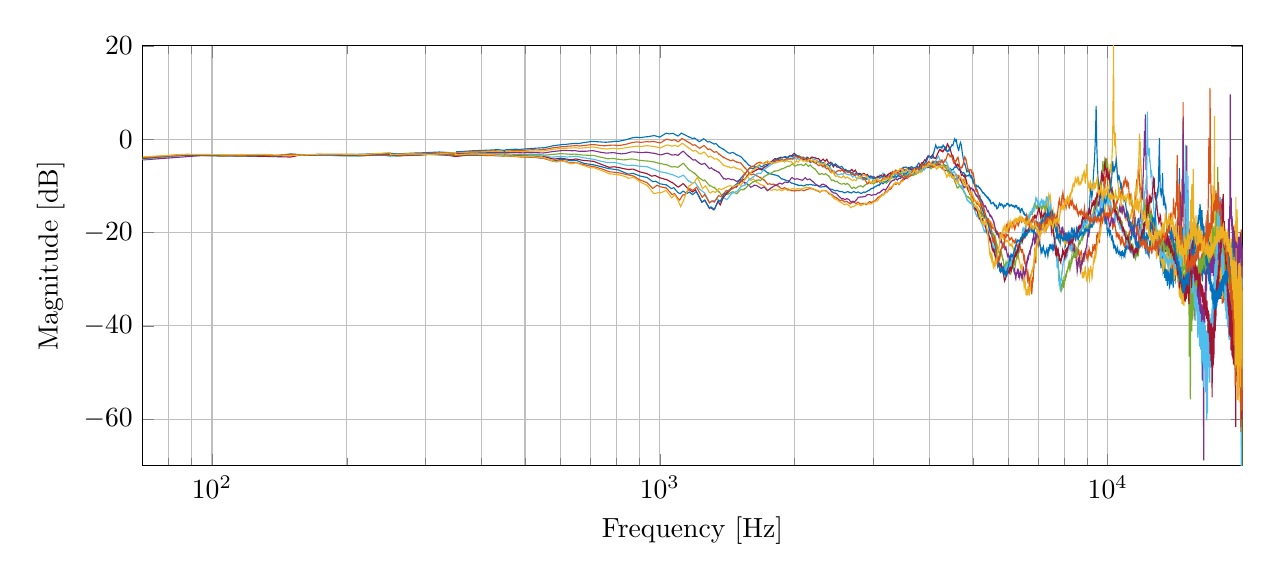
\begin{tikzpicture}

\begin{axis}[%
width=5.5in,
height=2.1in,
scale only axis,
xmin=70,
xmax=20000,
xmajorgrids,
xminorgrids,
ymajorgrids,
xmode=log,
xlabel={Frequency [Hz]},
ymin=-70,
ymax=20,
ylabel={Magnitude [dB]},
axis background/.style={fill=white},
title style={font=\bfseries},
%legend style={legend cell align=left,align=left,draw=white!15!black}
]
\addplot [color=mycolor1,solid]
  table[row sep=crcr]{%
0	-36.314\\
0.12467	-46.203\\
24.435	21.379\\
32.538	5.9252\\
32.663	-14.074\\
64.578	-4.5539\\
88.015	-3.4248\\
104.47	-3.5654\\
121.68	-3.4543\\
136.88	-3.5865\\
149.98	-3.1672\\
162.57	-3.418\\
172.29	-3.2875\\
194.48	-3.373\\
225.77	-3.1662\\
227.02	-3.1955\\
249.96	-3.0277\\
258.81	-3.1542\\
290.35	-2.9361\\
290.97	-2.9544\\
322.27	-2.7589\\
349.82	-2.9682\\
351.94	-2.6789\\
355.18	-2.7007\\
386.72	-2.4544\\
387.59	-2.4702\\
419.26	-2.3363\\
434.59	-2.2519\\
449.8	-2.412\\
451.67	-2.2926\\
475.61	-2.1575\\
487.45	-2.1991\\
516.25	-1.9911\\
517.5	-2.0042\\
548.41	-1.8421\\
549.66	-1.9003\\
580.58	-1.3752\\
581.7	-1.3778\\
610	-1.1191\\
613.74	-1.1339\\
644.91	-0.9135\\
659.99	-0.9434\\
677.32	-0.71792\\
677.57	-0.73619\\
703.87	-0.49587\\
710.61	-0.49507\\
741.9	-0.61847\\
758.23	-0.67409\\
773.19	-0.58822\\
774.31	-0.61185\\
797.75	-0.43973\\
807.97	-0.47363\\
838.76	-0.14306\\
838.76	-0.14306\\
871.05	0.32037\\
871.43	0.30951\\
888.51	0.40704\\
903.96	0.31934\\
935.13	0.52427\\
935.75	0.49481\\
967.17	0.72876\\
972.28	0.75514\\
998.21	0.4424\\
1000.1	0.45482\\
1031.4	1.2465\\
1033.2	1.2789\\
1049.6	1.118\\
1068.5	1.2526\\
1096.2	0.67767\\
1098.2	0.67326\\
1116.9	1.2894\\
1129.2	1.0559\\
1160.7	0.47145\\
1161.4	0.50833\\
1183.6	0.10439\\
1195.3	0.25274\\
1223.1	-0.53659\\
1226.5	-0.5376\\
1252.3	0.076714\\
1259.6	-0.079904\\
1280	-0.63319\\
1291.6	-0.51308\\
1321	-1.072\\
1334.2	-0.93898\\
1354.8	-1.6354\\
1355.4	-1.6052\\
1386.8	-2.2238\\
1387.8	-2.1735\\
1419.1	-2.9054\\
1434.9	-3.0411\\
1451.6	-2.8413\\
1455.4	-2.8282\\
1483.2	-3.359\\
1483.9	-3.3087\\
1515.1	-3.7658\\
1516.2	-3.7389\\
1547.1	-4.6825\\
1548.5	-4.641\\
1579.4	-5.5706\\
1580.7	-5.5612\\
1598.9	-5.867\\
1614.1	-5.7917\\
1645.2	-6.0847\\
1646.1	-6.0306\\
1677.5	-6.319\\
1678.1	-6.2583\\
1709.6	-6.7028\\
1710.2	-6.6481\\
1741.4	-7.2438\\
1742.5	-7.1849\\
1773.5	-7.5146\\
1774.3	-7.4538\\
1805.7	-7.6952\\
1806.7	-7.6472\\
1837.8	-7.9083\\
1838.7	-7.8712\\
1869.8	-8.5141\\
1872.4	-8.4724\\
1903.3	-8.7677\\
1904.4	-8.7327\\
1935.6	-9.0077\\
1936.6	-8.9502\\
1967.8	-9.4318\\
1970.6	-9.3852\\
1999.9	-9.6425\\
2000.7	-9.5858\\
2032	-9.8686\\
2032.7	-9.8107\\
2046.3	-9.9415\\
2065	-9.8735\\
2088.9	-10.034\\
2097.9	-10.017\\
2128.9	-9.7399\\
2140.7	-9.8191\\
2159.2	-9.7135\\
2168.2	-9.6978\\
2193.7	-9.8431\\
2198.5	-9.7955\\
2224.1	-9.9567\\
2243.1	-9.8538\\
2258.1	-10.008\\
2259.1	-9.9881\\
2283	-10.29\\
2292	-10.276\\
2319.7	-10.171\\
2324.1	-10.226\\
2342.6	-10.082\\
2355	-10.173\\
2386.4	-10.632\\
2387.3	-10.602\\
2418.6	-10.795\\
2421	-10.74\\
2451.7	-10.997\\
2466.7	-11.087\\
2481.8	-10.979\\
2487	-10.964\\
2516.2	-11.212\\
2519.2	-11.177\\
2530.8	-11.266\\
2549.2	-11.215\\
2580.4	-11.52\\
2584	-11.519\\
2611.8	-11.333\\
2627.7	-11.242\\
2644.6	-11.388\\
2645.7	-11.35\\
2674.6	-11.556\\
2678.5	-11.512\\
2707.8	-11.223\\
2709.9	-11.229\\
2740.9	-11.486\\
2744.4	-11.482\\
2768.6	-11.318\\
2775.5	-11.335\\
2805	-11.592\\
2817.5	-11.644\\
2835.8	-11.445\\
2838.8	-11.477\\
2853.8	-11.319\\
2872.6	-11.423\\
2902	-11.167\\
2903.3	-11.196\\
2932.6	-10.916\\
2936.7	-10.936\\
2966.2	-10.566\\
2970.5	-10.634\\
2999.9	-10.396\\
3000.7	-10.454\\
3026.6	-10.103\\
3033	-10.172\\
3064.2	-9.89\\
3065	-9.9438\\
3096.4	-9.7007\\
3097	-9.7991\\
3124.9	-9.2799\\
3130.2	-9.3215\\
3149	-9.5709\\
3161.4	-9.434\\
3185.5	-9.0127\\
3204.2	-9.1495\\
3225.9	-8.794\\
3225.9	-8.794\\
3256.6	-8.3887\\
3261.2	-8.436\\
3290.4	-7.8675\\
3291.6	-7.8868\\
3322.6	-7.0804\\
3326.1	-7.0644\\
3351.9	-7.2683\\
3355.1	-7.2297\\
3386.7	-6.7741\\
3390.1	-6.7601\\
3408.9	-6.9447\\
3419.6	-6.8298\\
3435.1	-6.6254\\
3453.7	-6.7621\\
3483.2	-6.2695\\
3484	-6.3027\\
3506.2	-5.9996\\
3524.7	-6.1292\\
3539.7	-5.9539\\
3548.7	-5.9851\\
3579.8	-6.3716\\
3581.3	-6.3339\\
3610.1	-6.5578\\
3613.1	-6.4099\\
3642.5	-6.6501\\
3658.5	-6.7048\\
3677.2	-6.3753\\
3677.7	-6.4332\\
3704	-6.1064\\
3710.4	-6.1813\\
3741.3	-5.8883\\
3742.4	-5.9308\\
3773.6	-5.2595\\
3786	-5.1197\\
3804.9	-5.5145\\
3807.3	-5.4579\\
3824.3	-5.6537\\
3840.6	-5.5798\\
3868.2	-5.327\\
3871.2	-5.3576\\
3902.7	-5.7829\\
3908	-5.8137\\
3932.4	-5.5254\\
3935.6	-5.5192\\
3950.8	-5.6721\\
3969.4	-5.5357\\
3999.1	-5.7697\\
4002	-5.7358\\
4014.9	-5.9048\\
4032.4	-5.8236\\
4064	-5.2081\\
4064.8	-5.2515\\
4094.3	-4.8822\\
4105.8	-4.8863\\
4121.8	-5.0187\\
4149.4	-4.8517\\
4161.2	-5.0069\\
4161.9	-4.9432\\
4192.9	-5.3928\\
4194.1	-5.3629\\
4225.2	-5.87\\
4226	-5.8222\\
4250.2	-5.9836\\
4259.1	-5.9897\\
4290.2	-5.6621\\
4291.2	-5.7012\\
4320.5	-5.4958\\
4322.7	-5.5156\\
4353.6	-5.7465\\
4360.9	-5.7663\\
4379.1	-5.6645\\
4388	-5.7363\\
4419.3	-6.2751\\
4420.2	-6.234\\
4451.4	-6.4405\\
4452.4	-6.4093\\
4472.8	-6.7306\\
4483.9	-6.6424\\
4496.9	-6.4865\\
4517.6	-6.5717\\
4546.9	-5.977\\
4563.7	-6.047\\
4580.7	-5.8874\\
4585.9	-5.84\\
4612.6	-6.1482\\
4612.9	-6.0941\\
4644	-6.535\\
4646.9	-6.51\\
4661.8	-6.6523\\
4678.5	-6.5704\\
4709.6	-6.9971\\
4710.7	-6.9599\\
4738.5	-7.3008\\
4742.4	-7.293\\
4760.7	-7.1615\\
4775.1	-7.2296\\
4806.2	-7.702\\
4806.7	-7.632\\
4836.2	-7.9937\\
4839.8	-7.9665\\
4856.7	-7.8053\\
4879.1	-7.8893\\
4903.3	-7.5773\\
4906.8	-7.5137\\
4934.5	-7.9549\\
4947.3	-7.8599\\
4967.1	-8.2645\\
4968.6	-8.2441\\
4998.3	-9.1058\\
5001.3	-9.0125\\
5032.2	-9.6375\\
5032.8	-9.5871\\
5059.1	-10.008\\
5083.3	-9.8492\\
5096.5	-10.128\\
5105.5	-10.245\\
5127.6	-10.042\\
5135.1	-9.9936\\
5160.5	-10.446\\
5165.2	-10.375\\
5193	-10.681\\
5193.8	-10.631\\
5224.7	-11.051\\
5227.4	-11.02\\
5257.1	-11.459\\
5261.2	-11.38\\
5288.9	-11.648\\
5291.8	-11.58\\
5319.3	-11.969\\
5323.9	-11.896\\
5354.8	-12.261\\
5355.5	-12.199\\
5383.4	-12.544\\
5388.1	-12.469\\
5419	-12.863\\
5419.5	-12.752\\
5449.5	-13.21\\
5452.1	-13.135\\
5483.1	-13.698\\
5484.1	-13.599\\
5490.1	-13.796\\
5516.9	-13.744\\
5546.6	-13.508\\
5550.1	-13.519\\
5579.5	-14.12\\
5584	-14.039\\
5592.1	-14.26\\
5614.2	-14.149\\
5645.2	-14.723\\
5647.9	-14.637\\
5654.3	-14.915\\
5680.9	-14.848\\
5708.7	-14.188\\
5711.3	-14.244\\
5730.2	-13.748\\
5757.6	-14.162\\
5772.9	-13.89\\
5779.7	-13.841\\
5804	-14.175\\
5813.9	-14.064\\
5838.1	-14.49\\
5851.9	-14.675\\
5865.5	-14.314\\
5871.2	-14.391\\
5879.7	-14.175\\
5909.2	-14.349\\
5934.9	-14.017\\
5935.8	-14.116\\
5967.2	-13.837\\
5974.1	-13.779\\
5996.3	-14.022\\
6000.9	-13.972\\
6026.7	-14.314\\
6032.8	-14.113\\
6060.7	-14.296\\
6065.7	-14.261\\
6087.8	-14.027\\
6098.7	-14.079\\
6126.7	-14.387\\
6136.9	-14.439\\
6147.1	-14.242\\
6162.7	-14.283\\
6190.9	-14.636\\
6194.2	-14.595\\
6217.4	-14.197\\
6228.8	-14.225\\
6240.9	-14.472\\
6260.9	-14.292\\
6290.2	-14.936\\
6301.1	-14.96\\
6319.8	-14.698\\
6326.8	-14.697\\
6354.4	-15.218\\
6355.4	-15.125\\
6381.2	-15.689\\
6388.1	-15.613\\
6412.3	-14.888\\
6419.6	-14.899\\
6450.7	-15.324\\
6451.7	-15.236\\
6480.7	-15.803\\
6485.2	-15.706\\
6514.5	-16.076\\
6517.4	-15.977\\
6546.7	-16.399\\
6557.5	-16.412\\
6579.6	-16.167\\
6585.1	-16.124\\
6612.6	-17.049\\
6613.4	-16.849\\
6642.8	-17.612\\
6645.4	-17.453\\
6659.1	-17.79\\
6688.5	-17.3\\
6709.6	-17.813\\
6709.7	-17.703\\
6740.9	-18.925\\
6743.5	-18.744\\
6770.9	-19.604\\
6788	-19.314\\
6804.9	-19.727\\
6807.5	-19.454\\
6829.8	-20.165\\
6857.5	-19.647\\
6871.1	-20.249\\
6871.8	-20.066\\
6890.4	-20.743\\
6907.6	-20.363\\
6935	-21.02\\
6935.8	-20.762\\
6967	-22.313\\
6968.2	-21.978\\
6999.5	-22.576\\
7009.9	-22.785\\
7032	-21.988\\
7046.5	-21.821\\
7064.5	-22.787\\
7065.7	-22.59\\
7095.2	-24.25\\
7110.7	-23.739\\
7127.6	-24.327\\
7130.9	-24.351\\
7158.7	-23.321\\
7174.5	-23.094\\
7191.3	-23.919\\
7196.1	-23.502\\
7223.4	-24.532\\
7226.2	-23.95\\
7251.9	-25.052\\
7259.3	-24.899\\
7290.1	-23.803\\
7306.1	-23.531\\
7319.6	-24.22\\
7323.8	-23.915\\
7351.6	-25.113\\
7355	-25.006\\
7386.4	-23.168\\
7389.2	-23.764\\
7409.7	-23.056\\
7422.7	-23.475\\
7443.2	-22.701\\
7460.9	-22.594\\
7479.9	-23.402\\
7494	-23.495\\
7512.7	-22.754\\
7519.7	-22.723\\
7540.3	-23.583\\
7552	-22.808\\
7576.2	-23.708\\
7581.4	-23.675\\
7610.8	-22.625\\
7613.2	-23.388\\
7644.5	-21.174\\
7645.4	-21.642\\
7675	-20.682\\
7681	-21.196\\
7703.2	-20.255\\
7715.9	-20.306\\
7727.4	-21.465\\
7746	-20.733\\
7773.6	-21.709\\
7778.4	-21.138\\
7798.6	-22.151\\
7806.6	-21.379\\
7832.5	-22.378\\
7839.6	-22.138\\
7870.5	-19.881\\
7871.6	-20.371\\
7897.4	-19.008\\
7908.2	-19.024\\
7933.8	-20.421\\
7936.3	-19.954\\
7964.4	-21.328\\
7968.6	-20.558\\
7999.9	-22.147\\
8004.2	-21.657\\
8024.7	-23.168\\
8033.8	-23.111\\
8063.1	-21.266\\
8066	-21.753\\
8095.3	-20.463\\
8114.7	-20.406\\
8126.3	-21.578\\
8129.8	-21.451\\
8155.8	-20.411\\
8164.7	-20.201\\
8188.7	-21.225\\
8194.9	-20.691\\
8211.7	-21.943\\
8225.9	-21.965\\
8255.6	-20.921\\
8258.1	-21.423\\
8289.3	-19.481\\
8292.1	-19.976\\
8314.3	-18.987\\
8325	-19.024\\
8354.5	-20.159\\
8363.4	-20.171\\
8382	-19.457\\
8388.3	-20.054\\
8414.1	-19.324\\
8419.4	-19.46\\
8450.6	-21.262\\
8464.9	-21.49\\
8483.5	-20.442\\
8484.4	-20.933\\
8515.9	-19.048\\
8526.4	-18.902\\
8545	-19.728\\
8559.3	-19.986\\
8579.6	-19.257\\
8582.5	-19.713\\
8602.9	-18.978\\
8617.1	-19.037\\
8641.3	-19.907\\
8650.2	-19.958\\
8676.2	-18.97\\
8677.9	-18.899\\
8709	-19.584\\
8710.6	-19.547\\
8740.3	-18.261\\
8742.7	-18.607\\
8774	-17.506\\
8777.6	-17.488\\
8803.4	-18.658\\
8814.1	-18.893\\
8838.2	-18.226\\
8838.9	-18.733\\
8870.5	-17.512\\
8871.1	-17.887\\
8895.2	-17.056\\
8913.9	-17.503\\
8934.4	-16.605\\
8937	-16.912\\
8952	-16.038\\
8983.4	-16.758\\
8998.6	-16.002\\
9001.1	-16.408\\
9030.4	-15.861\\
9033.4	-16.2\\
9052.1	-15.549\\
9072.4	-16.298\\
9096.4	-14.819\\
9097.5	-15.165\\
9128.7	-12.157\\
9129.4	-12.496\\
9160.4	-10.362\\
9163.9	-10.306\\
9193.6	-11.63\\
9194.1	-11.216\\
9213.1	-12.534\\
9225.9	-12.225\\
9256.7	-10.674\\
9259.3	-10.904\\
9290.4	-7.4853\\
9291	-7.6421\\
9322.6	-5.4423\\
9323.8	-5.8697\\
9354.7	-2.8839\\
9355.4	-3.2159\\
9386.8	1.0916\\
9387.7	0.65156\\
9419.4	7.1202\\
9419.4	7.1202\\
9451.5	-1.5727\\
9452.4	-1.2719\\
9484	-6.1289\\
9485.2	-5.7787\\
9514.4	-8.7361\\
9516.5	-8.3104\\
9548.4	-11.128\\
9549	-10.751\\
9580.5	-12.735\\
9592.7	-13.313\\
9612.9	-12.281\\
9619.3	-12.83\\
9645.2	-10.268\\
9663.2	-9.7774\\
9676.3	-11.178\\
9677.7	-10.999\\
9708.5	-13.365\\
9713.2	-13.139\\
9735.3	-14.514\\
9757.6	-13.806\\
9772.6	-14.451\\
9775.4	-14.134\\
9804.7	-16.134\\
9807.3	-15.846\\
9838.6	-17.375\\
9839.4	-17.118\\
9866.9	-18.114\\
9877.5	-18.089\\
9902	-16.841\\
9905.5	-16.673\\
9934.8	-17.456\\
9935.5	-17.221\\
9966.7	-19.591\\
9967.9	-19.285\\
9991.7	-20.265\\
10002	-20.014\\
10032	-19.214\\
10033	-19.543\\
10060	-19.044\\
10065	-19.203\\
10095	-20.293\\
10099	-20.183\\
10112	-19.532\\
10130	-19.551\\
10161	-20.614\\
10162	-20.301\\
10191	-21.595\\
10204	-21.621\\
10223	-21.134\\
10229	-21.063\\
10257	-21.84\\
10262	-21.601\\
10287	-22.423\\
10292	-22.158\\
10320	-22.859\\
10328	-22.595\\
10350	-23.144\\
10356	-23.179\\
10361	-22.74\\
10390	-22.854\\
10419	-23.857\\
10420	-23.461\\
10446	-24.44\\
10453	-24.418\\
10482	-23.699\\
10485	-23.986\\
10511	-23.331\\
10518	-23.297\\
10548	-24.4\\
10548	-24.126\\
10569	-24.602\\
10581	-24.569\\
10593	-24.046\\
10614	-24.037\\
10640	-24.638\\
10648	-24.317\\
10674	-24.937\\
10679	-24.93\\
10709	-24.278\\
10714	-24.248\\
10742	-24.794\\
10746	-24.922\\
10772	-24.121\\
10780	-24.07\\
10802	-24.898\\
10827	-24.949\\
10835	-24.406\\
10853	-24.363\\
10863	-24.775\\
10883	-24.339\\
10900	-25.024\\
10918	-25.158\\
10933	-24.286\\
10935	-24.588\\
10967	-23.008\\
10978	-22.83\\
10995	-23.394\\
11016	-23.523\\
11024	-23.023\\
11034	-23.414\\
11063	-22.692\\
11074	-22.687\\
11094	-23.217\\
11100	-23.194\\
11124	-22.657\\
11130	-22.969\\
11158	-22.439\\
11167	-22.83\\
11194	-22.047\\
11194	-22.293\\
11225	-21.375\\
11226	-21.728\\
11254	-20.894\\
11259	-20.899\\
11281	-21.443\\
11291	-21.343\\
11322	-19.611\\
11323	-19.977\\
11348	-18.928\\
11362	-18.816\\
11379	-19.647\\
11390	-19.701\\
11418	-18.876\\
11420	-19.214\\
11452	-17.952\\
11452	-18.274\\
11468	-17.728\\
11484	-18.231\\
11515	-16.885\\
11521	-16.692\\
11548	-18.233\\
11549	-17.981\\
11580	-19.257\\
11581	-18.732\\
11598	-19.398\\
11613	-19.189\\
11644	-18.32\\
11648	-18.801\\
11676	-17.231\\
11682	-17.872\\
11696	-17.008\\
11735	-17.008\\
11741	-17.732\\
11742	-17.349\\
11773	-19.38\\
11777	-18.983\\
11805	-21.096\\
11809	-21.179\\
11838	-19.338\\
11852	-19.057\\
11871	-20.165\\
11874	-19.448\\
11896	-20.48\\
11905	-19.96\\
11932	-21.687\\
11939	-21.612\\
11952	-20.48\\
11973	-19.827\\
11989	-21.605\\
12024	-21.676\\
12032	-20.151\\
12032	-20.402\\
12036	-21.616\\
12073	-18.587\\
12088	-21.593\\
12103	-20.836\\
12127	-23.135\\
12130	-22.324\\
12158	-23.905\\
12173	-24.607\\
12192	-21.63\\
12197	-22.298\\
12219	-20.322\\
12226	-20.344\\
12258	-23.126\\
12260	-22.035\\
12288	-24.726\\
12291	-24.822\\
12317	-23.148\\
12333	-23.574\\
12350	-25.11\\
12364	-25.22\\
12387	-23.233\\
12389	-24.247\\
12408	-21.774\\
12438	-23.705\\
12451	-21.452\\
12455	-22.988\\
12482	-19.463\\
12485	-20.047\\
12516	-23.458\\
12532	-23.686\\
12535	-21.638\\
12552	-23.353\\
12578	-20.964\\
12581	-21.177\\
12602	-23.074\\
12619	-23.116\\
12626	-20.732\\
12646	-22.788\\
12672	-18.924\\
12692	-18.139\\
12709	-20.225\\
12711	-18.663\\
12716	-20.773\\
12759	-18.294\\
12771	-20.011\\
12782	-20.077\\
12802	-18.124\\
12807	-18.545\\
12838	-22.506\\
12839	-21.306\\
12870	-23.244\\
12873	-22.087\\
12899	-23.885\\
12923	-21.964\\
12924	-23.75\\
12951	-23.584\\
12954	-21.796\\
12970	-21.818\\
12999	-23.574\\
13017	-24.019\\
13021	-22.403\\
13032	-22.785\\
13063	-25.412\\
13068	-24.26\\
13093	-26.351\\
13098	-24.973\\
13120	-27.058\\
13140	-25.814\\
13141	-27.681\\
13162	-27.294\\
13191	-24.315\\
13194	-24.53\\
13216	-25.959\\
13233	-24.892\\
13256	-27.667\\
13258	-26.559\\
13286	-28.237\\
13300	-27.986\\
13313	-25.9\\
13328	-26.345\\
13355	-28.793\\
13370	-27.602\\
13380	-29.733\\
13393	-29.121\\
13409	-27.137\\
13431	-27.1\\
13448	-28.769\\
13452	-27.607\\
13482	-30.277\\
13507	-30.261\\
13514	-28.448\\
13525	-29.693\\
13536	-27.933\\
13549	-28.409\\
13578	-30.902\\
13587	-31.455\\
13611	-29.674\\
13615	-31.044\\
13641	-28.043\\
13645	-28.983\\
13675	-26.617\\
13678	-26.862\\
13710	-30.39\\
13718	-29.419\\
13732	-31.767\\
13746	-31.65\\
13772	-29.403\\
13774	-31.363\\
13806	-28.133\\
13816	-27.543\\
13839	-30.002\\
13863	-28.726\\
13868	-30.837\\
13884	-30.917\\
13898	-28.64\\
13904	-30.005\\
13930	-27.302\\
13957	-27.453\\
13965	-29.484\\
13971	-28.338\\
13996	-31.464\\
14003	-31.823\\
14030	-28.025\\
14033	-29.96\\
14062	-25.931\\
14065	-27.496\\
14078	-25.313\\
14098	-25.61\\
14127	-30.125\\
14142	-30.296\\
14159	-27.652\\
14162	-29.541\\
14194	-24.94\\
14198	-26.427\\
14219	-23.79\\
14231	-23.707\\
14250	-26.08\\
14261	-26.211\\
14288	-21.728\\
14291	-23.082\\
14321	-18.677\\
14335	-16.758\\
14352	-20.271\\
14359	-17.355\\
14380	-22.406\\
14388	-21.624\\
14418	-15.856\\
14420	-16.875\\
14450	-6.7422\\
14452	-6.2176\\
14479	-14.416\\
14496	-16.493\\
14514	-12.628\\
14523	-11.243\\
14546	-17.331\\
14549	-14.852\\
14567	-18.998\\
14590	-13.564\\
14612	-19.959\\
14617	-16.765\\
14637	-22.752\\
14671	-22.674\\
14676	-20.046\\
14687	-19.553\\
14696	-22.681\\
14711	-18.911\\
14740	-22.775\\
14746	-21.438\\
14771	-23.683\\
14781	-21.534\\
14801	-24.084\\
14809	-21.251\\
14828	-23.876\\
14840	-21.96\\
14867	-24.856\\
14875	-25.692\\
14895	-22.554\\
14919	-23.909\\
14935	-26.659\\
14942	-24.024\\
14948	-26.313\\
14969	-24.074\\
14992	-27.04\\
15013	-26.939\\
15019	-24.33\\
15036	-27.301\\
15062	-24.414\\
15082	-25.974\\
15094	-23.403\\
15106	-25.599\\
15107	-23.244\\
15133	-23.2\\
15159	-26.556\\
15180	-28.229\\
15192	-24.959\\
15200	-26.991\\
15224	-22.841\\
15228	-24.31\\
15254	-21.491\\
15266	-20.527\\
15290	-23.058\\
15291	-21.752\\
15322	-25.427\\
15341	-25.718\\
15345	-24.17\\
15364	-24.027\\
15369	-25.761\\
15391	-25.672\\
15418	-22.191\\
15421	-22.8\\
15452	-18.014\\
15454	-17.888\\
15484	-21.9\\
15491	-23.052\\
15507	-21.079\\
15519	-21.628\\
15540	-23.988\\
15548	-23.503\\
15579	-20.876\\
15581	-20.786\\
15612	-23.109\\
15614	-22.012\\
15638	-24.386\\
15651	-24.031\\
15673	-20.345\\
15679	-21.138\\
15706	-23.793\\
15710	-22.721\\
15740	-25.57\\
15763	-25.702\\
15767	-23.894\\
15786	-25.406\\
15787	-24.085\\
15813	-25.123\\
15834	-22.261\\
15843	-23.965\\
15863	-21.908\\
15875	-22.154\\
15901	-24.916\\
15904	-23.466\\
15933	-25.957\\
15939	-24.798\\
15961	-27.553\\
15978	-25.227\\
16000	-28.007\\
16001	-26.29\\
16021	-29.366\\
16033	-27.555\\
16064	-30.181\\
16069	-28.203\\
16071	-31.114\\
16099	-29.743\\
16128	-27.276\\
16132	-28.802\\
16160	-26.271\\
16167	-26.342\\
16186	-28.575\\
16209	-26.856\\
16224	-29.394\\
16236	-27.378\\
16243	-29.651\\
16259	-27.318\\
16279	-30.487\\
16291	-29.1\\
16311	-26.551\\
16326	-28.225\\
16353	-25.255\\
16369	-25.571\\
16371	-28.169\\
16389	-26.335\\
16400	-28.749\\
16423	-26.475\\
16450	-28.296\\
16467	-29.033\\
16481	-26.54\\
16494	-28.092\\
16514	-23.373\\
16518	-24.725\\
16541	-22.307\\
16561	-23.782\\
16571	-22.156\\
16596	-23.42\\
16610	-21.145\\
16628	-22.039\\
16644	-20.293\\
16645	-21.197\\
16673	-17.65\\
16678	-18.593\\
16705	-16.495\\
16715	-15.863\\
16728	-18.649\\
16747	-17.22\\
16752	-20.1\\
16778	-18.282\\
16803	-20.994\\
16819	-22.842\\
16822	-19.571\\
16848	-21.634\\
16866	-19.309\\
16889	-18.091\\
16893	-20.758\\
16910	-18.875\\
16913	-20.936\\
16936	-21.9\\
16939	-18.983\\
16974	-20.101\\
16983	-22.185\\
17007	-22.597\\
17010	-19.267\\
17054	-20.527\\
17057	-23.168\\
17080	-22.567\\
17081	-20.191\\
17104	-19.464\\
17127	-23.2\\
17129	-20.943\\
17161	-23.72\\
17171	-22.675\\
17177	-25.12\\
17213	-24.576\\
17221	-22.109\\
17227	-22.572\\
17241	-25.379\\
17264	-24.911\\
17265	-22.352\\
17312	-21.088\\
17315	-24.439\\
17338	-24.125\\
17349	-22.132\\
17362	-21.983\\
17382	-25.16\\
17397	-24.757\\
17409	-22.839\\
17432	-25.015\\
17449	-21.73\\
17453	-23.475\\
17482	-19.473\\
17495	-19.082\\
17503	-21.952\\
17526	-19.344\\
17546	-23.171\\
17550	-21.013\\
17570	-25.487\\
17596	-24.184\\
17602	-20.467\\
17620	-19.184\\
17645	-23.834\\
17651	-23.832\\
17664	-20.589\\
17679	-21.745\\
17687	-26.258\\
17711	-22.868\\
17737	-27.513\\
17758	-24.317\\
17761	-28.047\\
17793	-27.887\\
17805	-25.063\\
17823	-29.104\\
17828	-25.092\\
17839	-26.141\\
17863	-29.576\\
17875	-27.674\\
17898	-31.741\\
17922	-28.879\\
17927	-32.113\\
17941	-32.371\\
17952	-29.731\\
17969	-33.194\\
17995	-29.292\\
18016	-33.262\\
18026	-29.765\\
18039	-29.8\\
18063	-32.972\\
18066	-30.218\\
18089	-34.982\\
18103	-31.024\\
18109	-33.739\\
18136	-30.389\\
18159	-33.522\\
18163	-31.281\\
18183	-34.353\\
18203	-33.983\\
18206	-30.627\\
18227	-31.012\\
18254	-34.144\\
18259	-32.354\\
18289	-34.958\\
18300	-35.248\\
18315	-32.195\\
18324	-36.319\\
18326	-32.639\\
18364	-35.341\\
18367	-32.355\\
18391	-31.901\\
18415	-35.779\\
18431	-32.206\\
18438	-36.197\\
18465	-35.678\\
18475	-32.337\\
18485	-32.191\\
18489	-35.268\\
18532	-32.663\\
18535	-35.674\\
18558	-36.238\\
18579	-32.176\\
18605	-35.962\\
18606	-32.168\\
18624	-32.692\\
18629	-36.096\\
18647	-32.878\\
18649	-37.131\\
18688	-36.642\\
18691	-33.273\\
18720	-33.21\\
18724	-35.869\\
18746	-32.875\\
18770	-37.03\\
18778	-33.087\\
18780	-35.876\\
18837	-35.137\\
18838	-32.353\\
18839	-32.012\\
18860	-35.322\\
18881	-35.48\\
18885	-32.396\\
18910	-31.927\\
18934	-37.657\\
18941	-35.889\\
18947	-32.526\\
18990	-32.128\\
18992	-34.43\\
19001	-31.205\\
19028	-34.951\\
19041	-37.442\\
19051	-31.767\\
19071	-32.179\\
19080	-35.185\\
19098	-31.953\\
19115	-35.453\\
19139	-35.683\\
19141	-30.624\\
19168	-35.963\\
19192	-31.208\\
19199	-36.299\\
19215	-31.559\\
19236	-35.486\\
19241	-29.437\\
19262	-35.001\\
19281	-30.947\\
19309	-30.802\\
19319	-34.395\\
19340	-30.206\\
19341	-36.44\\
19369	-33.938\\
19376	-28.824\\
19389	-32.743\\
19403	-28.519\\
19420	-28.523\\
19447	-34.102\\
19473	-34.435\\
19476	-28.04\\
19494	-28.231\\
19512	-33.016\\
19545	-28.992\\
19545	-33.887\\
19562	-32.824\\
19564	-27.239\\
19587	-27.468\\
19588	-34.397\\
19636	-33.078\\
19638	-27.594\\
19652	-33.555\\
19671	-27.012\\
19685	-36.693\\
19708	-25.152\\
19710	-30.372\\
19732	-24.006\\
19752	-25.067\\
19754	-30.043\\
19778	-25.353\\
19799	-32.274\\
19822	-35.328\\
19825	-26.563\\
19846	-26.86\\
19849	-34.365\\
19873	-28.366\\
19887	-34.629\\
19919	-28.418\\
19935	-36.242\\
19963	-37.528\\
19966	-30.074\\
19983	-37.412\\
19990	-28.591\\
20010	-41.127\\
20030	-32.098\\
20033	-31.579\\
20036	-43.567\\
20080	-30.784\\
20086	-39.487\\
20099	-38.914\\
20127	-32.586\\
20154	-42.3\\
20157	-32.623\\
20174	-42.864\\
20177	-31.543\\
20204	-39.028\\
20224	-30.335\\
20245	-41.396\\
20248	-32.364\\
20268	-33.188\\
20271	-39.813\\
20292	-32.89\\
20320	-40.346\\
20338	-42.495\\
20342	-32.904\\
20362	-42.066\\
20385	-34.256\\
20409	-40.16\\
20415	-33.838\\
20432	-31.106\\
20439	-38.522\\
20456	-40.098\\
20479	-31.528\\
20503	-38.127\\
20506	-31.366\\
20529	-40.749\\
20543	-32.571\\
20563	-38.239\\
20576	-31.392\\
20596	-32.261\\
20605	-39.359\\
20620	-39.539\\
20623	-31.145\\
20646	-32.6\\
20667	-40.049\\
20690	-39.754\\
20693	-32.789\\
20714	-31.802\\
20740	-40.303\\
20750	-39.842\\
20761	-31.958\\
20803	-37.765\\
20805	-32.626\\
20808	-30.094\\
20829	-38.752\\
20858	-39.398\\
20859	-32.962\\
20878	-39.513\\
20881	-31.582\\
20913	-33.001\\
20934	-41.557\\
20944	-39.351\\
20948	-32.991\\
20977	-35.256\\
21000	-40.968\\
21001	-35.329\\
21022	-46.017\\
21041	-35.138\\
21049	-42.383\\
21069	-45.42\\
21092	-34.794\\
21113	-43.06\\
21116	-33.838\\
21136	-47.009\\
21139	-35.224\\
21183	-53.229\\
21188	-36.828\\
21197	-37.616\\
21200	-44.635\\
21253	-48.21\\
21256	-36.943\\
21277	-36.074\\
21280	-46.06\\
21303	-36.279\\
21306	-49.268\\
21327	-36.786\\
21354	-46.762\\
21371	-37.728\\
21374	-49.554\\
21394	-38.978\\
21397	-55.995\\
21438	-48.779\\
21444	-37.686\\
21468	-37.028\\
21479	-46.672\\
21491	-49.08\\
21512	-36.81\\
21532	-39.076\\
21541	-48.692\\
21552	-39.667\\
21562	-56.663\\
21582	-38.457\\
21585	-54.809\\
21632	-50.584\\
21639	-39.137\\
21652	-38.44\\
21676	-49.177\\
21697	-47.944\\
21699	-37.992\\
21733	-47.798\\
21739	-39.668\\
21770	-53.716\\
21773	-38.535\\
21775	-39.965\\
21805	-52.801\\
21817	-37.917\\
21823	-49.12\\
21840	-37.284\\
21867	-49.541\\
21888	-53.464\\
21890	-37.986\\
21918	-50.615\\
21934	-39.2\\
21937	-36.281\\
21945	-56.606\\
21978	-58.85\\
21984	-35.946\\
22020	-53.902\\
22028	-36.763\\
22037	-57.612\\
22039	-37.461\\
22070	-60.953\\
22078	-35.126\\
22098	-34.456\\
22103	-57.8\\
22148	-37.428\\
22156	-58.687\\
22172	-39.112\\
22189	-74.275\\
22194	-67.533\\
22216	-37.738\\
22234	-72.683\\
22242	-35.973\\
22259	-85.489\\
22289	-33.573\\
22304	-79.455\\
22309	-35.034\\
22333	-34.185\\
22340	-78.599\\
22359	-33.654\\
22386	-69.283\\
22403	-30.626\\
22415	-62.492\\
22431	-68.652\\
22450	-27.824\\
22473	-28.371\\
22480	-69.301\\
22485	-57.014\\
22497	-25.882\\
22523	-24.373\\
22542	-59.333\\
22569	-67.681\\
22570	-30.059\\
22587	-62.437\\
22591	-29.717\\
22614	-24.556\\
22621	-54.859\\
22664	-25.51\\
22665	-58.522\\
22685	-27.132\\
22697	-55.284\\
22721	-61.927\\
22732	-28.77\\
22752	-59.755\\
22755	-28.574\\
22777	-59.807\\
22781	-29.823\\
22825	-29.864\\
22836	-66.407\\
22849	-29.262\\
22866	-69.26\\
22872	-28.557\\
22903	-69.596\\
22911	-69.905\\
22922	-31.205\\
22957	-66.797\\
22966	-31.93\\
22972	-65.137\\
22993	-30.533\\
23019	-34.186\\
23025	-59.261\\
23044	-74.035\\
23060	-31.523\\
23083	-32.672\\
23086	-63.347\\
23110	-32.013\\
23117	-59.75\\
23130	-33.048\\
23154	-69.906\\
23175	-61.589\\
23177	-32.88\\
23212	-68.361\\
23224	-31.453\\
23243	-59.948\\
23251	-33.392\\
23261	-75.347\\
23274	-32.891\\
23318	-33.315\\
23318	-66.141\\
23342	-31.559\\
23349	-59.827\\
23377	-62.919\\
23382	-35.147\\
23400	-62.163\\
23412	-32.063\\
23435	-33.776\\
23445	-61.147\\
23462	-32.656\\
23462	-62.798\\
23485	-33.813\\
23499	-65.653\\
23545	-36.628\\
23546	-69.89\\
23555	-64.912\\
23576	-30.278\\
23589	-61.917\\
23600	-31.251\\
23626	-33.901\\
23633	-75.548\\
23649	-60.583\\
23670	-30.678\\
23692	-66.67\\
23697	-32.507\\
23717	-31.746\\
23740	-86.392\\
23747	-34.065\\
23772	-66.823\\
23782	-58.342\\
23787	-30.807\\
23811	-27.416\\
23818	-55.223\\
23861	-31.366\\
23868	-62.718\\
23878	-58.464\\
23899	-33.571\\
23931	-30.13\\
23934	-64.364\\
23945	-23.509\\
23954	-69.152\\
23975	-30.528\\
23980	-62.777\\
24020	-62.777\\
24025	-30.528\\
24046	-69.152\\
24055	-23.509\\
24066	-64.364\\
24069	-30.13\\
24101	-33.571\\
24122	-58.464\\
24132	-62.718\\
24139	-31.366\\
24182	-55.223\\
24189	-27.416\\
24213	-30.807\\
24218	-58.342\\
24228	-66.823\\
24253	-34.065\\
24260	-86.392\\
24283	-31.746\\
24303	-32.507\\
24308	-66.67\\
24330	-30.678\\
24351	-60.583\\
24367	-75.548\\
24374	-33.901\\
24400	-31.251\\
24411	-61.917\\
24424	-30.278\\
24445	-64.912\\
24454	-69.89\\
24455	-36.628\\
24501	-65.653\\
24515	-33.813\\
24538	-62.798\\
24538	-32.656\\
24555	-61.147\\
24565	-33.776\\
24588	-32.063\\
24600	-62.163\\
24618	-35.147\\
24623	-62.919\\
24651	-59.827\\
24658	-31.559\\
24682	-66.141\\
24682	-33.315\\
24726	-32.891\\
24739	-75.347\\
24749	-33.392\\
24757	-59.948\\
24776	-31.453\\
24788	-68.361\\
24823	-32.88\\
24825	-61.589\\
24846	-69.906\\
24870	-33.048\\
24883	-59.75\\
24890	-32.013\\
24914	-63.347\\
24917	-32.672\\
24940	-31.523\\
24956	-74.035\\
24975	-59.261\\
24981	-34.186\\
25007	-30.533\\
25028	-65.137\\
25034	-31.93\\
25043	-66.797\\
25078	-31.205\\
25089	-69.905\\
25097	-69.596\\
25128	-28.557\\
25134	-69.26\\
25151	-29.262\\
25164	-66.407\\
25175	-29.864\\
25219	-29.823\\
25223	-59.807\\
25245	-28.574\\
25248	-59.755\\
25268	-28.77\\
25279	-61.927\\
25303	-55.284\\
25315	-27.132\\
25335	-58.522\\
25336	-25.51\\
25379	-54.859\\
25386	-24.556\\
25409	-29.717\\
25413	-62.437\\
25430	-30.059\\
25431	-67.681\\
25458	-59.333\\
25477	-24.373\\
25503	-25.882\\
25515	-57.014\\
25520	-69.301\\
25527	-28.371\\
25550	-27.824\\
25569	-68.652\\
25585	-62.492\\
25597	-30.626\\
25614	-69.283\\
25641	-33.654\\
25660	-78.599\\
25667	-34.185\\
25691	-35.034\\
25696	-79.455\\
25711	-33.573\\
25741	-85.489\\
25758	-35.973\\
25766	-72.683\\
25784	-37.738\\
25806	-67.533\\
25811	-74.275\\
25828	-39.112\\
25844	-58.687\\
25852	-37.428\\
25897	-57.8\\
25902	-34.456\\
25922	-35.126\\
25930	-60.953\\
25961	-37.461\\
25963	-57.612\\
25972	-36.763\\
25980	-53.902\\
26016	-35.946\\
26022	-58.85\\
26055	-56.606\\
26063	-36.281\\
26066	-39.2\\
26082	-50.615\\
26110	-37.986\\
26112	-53.464\\
26133	-49.541\\
26160	-37.284\\
26177	-49.12\\
26183	-37.917\\
26195	-52.801\\
26225	-39.965\\
26227	-38.535\\
26230	-53.716\\
26261	-39.668\\
26267	-47.798\\
26301	-37.992\\
26303	-47.944\\
26324	-49.177\\
26348	-38.44\\
26361	-39.137\\
26368	-50.584\\
26415	-54.809\\
26418	-38.457\\
26438	-56.663\\
26448	-39.667\\
26459	-48.692\\
26468	-39.076\\
26488	-36.81\\
26509	-49.08\\
26521	-46.672\\
26532	-37.028\\
26556	-37.686\\
26562	-48.779\\
26603	-55.995\\
26606	-38.978\\
26626	-49.554\\
26629	-37.728\\
26646	-46.762\\
26673	-36.786\\
26694	-49.268\\
26697	-36.279\\
26720	-46.06\\
26723	-36.074\\
26744	-36.943\\
26747	-48.21\\
26800	-44.635\\
26803	-37.616\\
26812	-36.828\\
26817	-53.229\\
26861	-35.224\\
26864	-47.009\\
26884	-33.838\\
26887	-43.06\\
26908	-34.794\\
26931	-45.42\\
26951	-42.383\\
26959	-35.138\\
26978	-46.017\\
26999	-35.329\\
27000	-40.968\\
27023	-35.256\\
27052	-32.991\\
27056	-39.351\\
27066	-41.557\\
27087	-33.001\\
27119	-31.582\\
27122	-39.513\\
27141	-32.962\\
27142	-39.398\\
27171	-38.752\\
27192	-30.094\\
27195	-32.626\\
27197	-37.765\\
27239	-31.958\\
27250	-39.842\\
27260	-40.303\\
27286	-31.802\\
27307	-32.789\\
27310	-39.754\\
27333	-40.049\\
27354	-32.6\\
27377	-31.145\\
27380	-39.539\\
27395	-39.359\\
27404	-32.261\\
27424	-31.392\\
27437	-38.239\\
27457	-32.571\\
27471	-40.749\\
27494	-31.366\\
27497	-38.127\\
27521	-31.528\\
27544	-40.098\\
27561	-38.522\\
27568	-31.106\\
27585	-33.838\\
27591	-40.16\\
27615	-34.256\\
27638	-42.066\\
27658	-32.904\\
27662	-42.495\\
27680	-40.346\\
27708	-32.89\\
27729	-39.813\\
27732	-33.188\\
27752	-32.364\\
27755	-41.396\\
27776	-30.335\\
27796	-39.028\\
27823	-31.543\\
27826	-42.864\\
27843	-32.623\\
27846	-42.3\\
27873	-32.586\\
27901	-38.914\\
27914	-39.487\\
27920	-30.784\\
27964	-43.567\\
27967	-31.579\\
27970	-32.098\\
27990	-41.127\\
28010	-28.591\\
28017	-37.412\\
28034	-30.074\\
28037	-37.528\\
28065	-36.242\\
28081	-28.418\\
28113	-34.629\\
28127	-28.366\\
28151	-34.365\\
28154	-26.86\\
28175	-26.563\\
28178	-35.328\\
28201	-32.274\\
28222	-25.353\\
28246	-30.043\\
28248	-25.067\\
28268	-24.006\\
28290	-30.372\\
28292	-25.152\\
28315	-36.693\\
28329	-27.012\\
28348	-33.555\\
28362	-27.594\\
28364	-33.078\\
28412	-34.397\\
28413	-27.468\\
28436	-27.239\\
28438	-32.824\\
28455	-33.887\\
28455	-28.992\\
28488	-33.016\\
28506	-28.231\\
28524	-28.04\\
28527	-34.435\\
28553	-34.102\\
28580	-28.523\\
28597	-28.519\\
28611	-32.743\\
28624	-28.824\\
28631	-33.938\\
28659	-36.44\\
28660	-30.206\\
28681	-34.395\\
28691	-30.802\\
28719	-30.947\\
28738	-35.001\\
28759	-29.437\\
28764	-35.486\\
28785	-31.559\\
28801	-36.299\\
28808	-31.208\\
28832	-35.963\\
28859	-30.624\\
28861	-35.683\\
28885	-35.453\\
28902	-31.953\\
28920	-35.185\\
28929	-32.179\\
28949	-31.767\\
28959	-37.442\\
28972	-34.951\\
28999	-31.205\\
29008	-34.43\\
29010	-32.128\\
29053	-32.526\\
29059	-35.889\\
29066	-37.657\\
29090	-31.927\\
29115	-32.396\\
29119	-35.48\\
29140	-35.322\\
29161	-32.012\\
29162	-32.353\\
29163	-35.137\\
29220	-35.876\\
29222	-33.087\\
29230	-37.03\\
29254	-32.875\\
29276	-35.869\\
29280	-33.21\\
29309	-33.273\\
29312	-36.642\\
29351	-37.131\\
29353	-32.878\\
29371	-36.096\\
29376	-32.692\\
29394	-32.168\\
29395	-35.962\\
29421	-32.176\\
29442	-36.238\\
29465	-35.674\\
29468	-32.663\\
29511	-35.268\\
29515	-32.191\\
29525	-32.337\\
29535	-35.678\\
29562	-36.197\\
29569	-32.206\\
29585	-35.779\\
29609	-31.901\\
29633	-32.355\\
29636	-35.341\\
29674	-32.639\\
29676	-36.319\\
29685	-32.195\\
29700	-35.248\\
29711	-34.958\\
29741	-32.354\\
29746	-34.144\\
29773	-31.012\\
29794	-30.627\\
29797	-33.983\\
29817	-34.353\\
29837	-31.281\\
29841	-33.522\\
29864	-30.389\\
29891	-33.739\\
29897	-31.024\\
29911	-34.982\\
29934	-30.218\\
29937	-32.972\\
29961	-29.8\\
29974	-29.765\\
29984	-33.262\\
30005	-29.292\\
30031	-33.194\\
30048	-29.731\\
30059	-32.371\\
30073	-32.113\\
30078	-28.879\\
30102	-31.741\\
30125	-27.674\\
30137	-29.576\\
30161	-26.141\\
30172	-25.092\\
30177	-29.104\\
30195	-25.063\\
30207	-27.887\\
30239	-28.047\\
30242	-24.317\\
30263	-27.513\\
30289	-22.868\\
30313	-26.258\\
30321	-21.745\\
30336	-20.589\\
30349	-23.832\\
30355	-23.834\\
30380	-19.184\\
30398	-20.467\\
30404	-24.184\\
30430	-25.487\\
30450	-21.013\\
30454	-23.171\\
30474	-19.344\\
30497	-21.952\\
30505	-19.082\\
30518	-19.473\\
30547	-23.475\\
30551	-21.73\\
30568	-25.015\\
30591	-22.839\\
30603	-24.757\\
30618	-25.16\\
30638	-21.983\\
30651	-22.132\\
30662	-24.125\\
30685	-24.439\\
30688	-21.088\\
30735	-22.352\\
30736	-24.911\\
30759	-25.379\\
30773	-22.572\\
30779	-22.109\\
30787	-24.576\\
30823	-25.12\\
30829	-22.675\\
30839	-23.72\\
30871	-20.943\\
30873	-23.2\\
30896	-19.464\\
30919	-20.191\\
30920	-22.567\\
30943	-23.168\\
30946	-20.527\\
30990	-19.267\\
30993	-22.597\\
31017	-22.185\\
31026	-20.101\\
31061	-18.983\\
31064	-21.9\\
31087	-20.936\\
31090	-18.875\\
31107	-20.758\\
31111	-18.091\\
31134	-19.309\\
31152	-21.634\\
31178	-19.571\\
31181	-22.842\\
31197	-20.994\\
31222	-18.282\\
31248	-20.1\\
31253	-17.22\\
31272	-18.649\\
31285	-15.863\\
31295	-16.495\\
31322	-18.593\\
31327	-17.65\\
31355	-21.197\\
31356	-20.293\\
31372	-22.039\\
31390	-21.145\\
31404	-23.42\\
31429	-22.156\\
31439	-23.782\\
31459	-22.307\\
31482	-24.725\\
31486	-23.373\\
31506	-28.092\\
31519	-26.54\\
31533	-29.033\\
31550	-28.296\\
31577	-26.475\\
31600	-28.749\\
31611	-26.335\\
31629	-28.169\\
31631	-25.571\\
31647	-25.255\\
31674	-28.225\\
31689	-26.551\\
31709	-29.1\\
31721	-30.487\\
31741	-27.318\\
31757	-29.651\\
31764	-27.378\\
31776	-29.394\\
31791	-26.856\\
31814	-28.575\\
31833	-26.342\\
31840	-26.271\\
31868	-28.802\\
31872	-27.276\\
31901	-29.743\\
31929	-31.114\\
31931	-28.203\\
31936	-30.181\\
31967	-27.555\\
31979	-29.366\\
31999	-26.29\\
32000	-28.007\\
32022	-25.227\\
32039	-27.553\\
32061	-24.798\\
32067	-25.957\\
32096	-23.466\\
32099	-24.916\\
32125	-22.154\\
32137	-21.908\\
32157	-23.965\\
32166	-22.261\\
32187	-25.123\\
32213	-24.085\\
32214	-25.406\\
32233	-23.894\\
32237	-25.702\\
32260	-25.57\\
32290	-22.721\\
32294	-23.793\\
32321	-21.138\\
32327	-20.345\\
32349	-24.031\\
32362	-24.386\\
32386	-22.012\\
32388	-23.109\\
32419	-20.786\\
32421	-20.876\\
32452	-23.503\\
32460	-23.988\\
32481	-21.628\\
32493	-21.079\\
32509	-23.052\\
32516	-21.9\\
32546	-17.888\\
32548	-18.014\\
32579	-22.8\\
32582	-22.191\\
32609	-25.672\\
32631	-25.761\\
32636	-24.027\\
32655	-24.17\\
32659	-25.718\\
32678	-25.427\\
32709	-21.752\\
32710	-23.058\\
32734	-20.527\\
32746	-21.491\\
32772	-24.31\\
32776	-22.841\\
32800	-26.991\\
32808	-24.959\\
32820	-28.229\\
32841	-26.556\\
32867	-23.2\\
32893	-23.244\\
32894	-25.599\\
32906	-23.403\\
32918	-25.974\\
32938	-24.414\\
32964	-27.301\\
32981	-24.33\\
32987	-26.939\\
33008	-27.04\\
33031	-24.074\\
33052	-26.313\\
33058	-24.024\\
33065	-26.659\\
33081	-23.909\\
33105	-22.554\\
33125	-25.692\\
33133	-24.856\\
33160	-21.96\\
33172	-23.876\\
33191	-21.251\\
33199	-24.084\\
33219	-21.534\\
33229	-23.683\\
33254	-21.438\\
33260	-22.775\\
33289	-18.911\\
33304	-22.681\\
33313	-19.553\\
33324	-20.046\\
33329	-22.674\\
33363	-22.752\\
33383	-16.765\\
33388	-19.959\\
33410	-13.564\\
33433	-18.998\\
33451	-14.852\\
33454	-17.331\\
33477	-11.243\\
33486	-12.628\\
33504	-16.493\\
33521	-14.416\\
33548	-6.2176\\
33550	-6.7422\\
33580	-16.875\\
33582	-15.856\\
33612	-21.624\\
33620	-22.406\\
33641	-17.355\\
33648	-20.271\\
33665	-16.758\\
33679	-18.677\\
33709	-23.082\\
33712	-21.728\\
33739	-26.211\\
33750	-26.08\\
33769	-23.707\\
33781	-23.79\\
33802	-26.427\\
33806	-24.94\\
33838	-29.541\\
33841	-27.652\\
33858	-30.296\\
33873	-30.125\\
33902	-25.61\\
33922	-25.313\\
33935	-27.496\\
33938	-25.931\\
33967	-29.96\\
33970	-28.025\\
33997	-31.823\\
34004	-31.464\\
34029	-28.338\\
34035	-29.484\\
34043	-27.453\\
34070	-27.302\\
34096	-30.005\\
34102	-28.64\\
34116	-30.917\\
34132	-30.837\\
34137	-28.726\\
34161	-30.002\\
34184	-27.543\\
34194	-28.133\\
34226	-31.363\\
34228	-29.403\\
34254	-31.65\\
34268	-31.767\\
34282	-29.419\\
34290	-30.39\\
34322	-26.862\\
34325	-26.617\\
34355	-28.983\\
34359	-28.043\\
34385	-31.044\\
34389	-29.674\\
34413	-31.455\\
34422	-30.902\\
34451	-28.409\\
34464	-27.933\\
34475	-29.693\\
34486	-28.448\\
34493	-30.261\\
34518	-30.277\\
34548	-27.607\\
34552	-28.769\\
34569	-27.1\\
34591	-27.137\\
34607	-29.121\\
34620	-29.733\\
34630	-27.602\\
34645	-28.793\\
34672	-26.345\\
34687	-25.9\\
34700	-27.986\\
34714	-28.237\\
34742	-26.559\\
34744	-27.667\\
34767	-24.892\\
34784	-25.959\\
34806	-24.53\\
34809	-24.315\\
34838	-27.294\\
34859	-27.681\\
34860	-25.814\\
34880	-27.058\\
34902	-24.973\\
34907	-26.351\\
34932	-24.26\\
34937	-25.412\\
34968	-22.785\\
34979	-22.403\\
34983	-24.019\\
35001	-23.574\\
35030	-21.818\\
35046	-21.796\\
35049	-23.584\\
35076	-23.75\\
35077	-21.964\\
35101	-23.885\\
35127	-22.087\\
35130	-23.244\\
35161	-21.306\\
35162	-22.506\\
35193	-18.545\\
35198	-18.124\\
35218	-20.077\\
35229	-20.011\\
35241	-18.294\\
35284	-20.773\\
35289	-18.663\\
35291	-20.225\\
35308	-18.139\\
35328	-18.924\\
35354	-22.788\\
35374	-20.732\\
35381	-23.116\\
35398	-23.074\\
35419	-21.177\\
35422	-20.964\\
35448	-23.353\\
35465	-21.638\\
35468	-23.686\\
35484	-23.458\\
35515	-20.047\\
35518	-19.463\\
35545	-22.988\\
35549	-21.452\\
35562	-23.705\\
35592	-21.774\\
35611	-24.247\\
35613	-23.233\\
35636	-25.22\\
35650	-25.11\\
35667	-23.574\\
35683	-23.148\\
35709	-24.822\\
35712	-24.726\\
35740	-22.035\\
35742	-23.126\\
35774	-20.344\\
35781	-20.322\\
35803	-22.298\\
35808	-21.63\\
35827	-24.607\\
35842	-23.905\\
35870	-22.324\\
35873	-23.135\\
35897	-20.836\\
35912	-21.593\\
35927	-18.587\\
35964	-21.616\\
35968	-20.402\\
35968	-20.151\\
35976	-21.676\\
36011	-21.605\\
36027	-19.827\\
36048	-20.48\\
36061	-21.612\\
36068	-21.687\\
36095	-19.96\\
36104	-20.48\\
36126	-19.448\\
36129	-20.165\\
36148	-19.057\\
36162	-19.338\\
36191	-21.179\\
36195	-21.096\\
36223	-18.983\\
36227	-19.38\\
36258	-17.349\\
36259	-17.732\\
36265	-17.008\\
36304	-17.008\\
36318	-17.872\\
36324	-17.231\\
36352	-18.801\\
36356	-18.32\\
36387	-19.189\\
36402	-19.398\\
36419	-18.732\\
36420	-19.257\\
36451	-17.981\\
36452	-18.233\\
36479	-16.692\\
36485	-16.885\\
36516	-18.231\\
36532	-17.728\\
36548	-18.274\\
36548	-17.952\\
36580	-19.214\\
36582	-18.876\\
36610	-19.701\\
36621	-19.647\\
36638	-18.816\\
36652	-18.928\\
36677	-19.977\\
36678	-19.611\\
36709	-21.343\\
36719	-21.443\\
36741	-20.899\\
36746	-20.894\\
36774	-21.728\\
36775	-21.375\\
36806	-22.293\\
36806	-22.047\\
36833	-22.83\\
36842	-22.439\\
36870	-22.969\\
36876	-22.657\\
36900	-23.194\\
36906	-23.217\\
36926	-22.687\\
36937	-22.692\\
36966	-23.414\\
36976	-23.023\\
36984	-23.523\\
37005	-23.394\\
37022	-22.83\\
37033	-23.008\\
37065	-24.588\\
37067	-24.286\\
37082	-25.158\\
37100	-25.024\\
37117	-24.339\\
37137	-24.775\\
37147	-24.363\\
37165	-24.406\\
37173	-24.949\\
37198	-24.898\\
37220	-24.07\\
37228	-24.121\\
37254	-24.922\\
37258	-24.794\\
37286	-24.248\\
37291	-24.278\\
37321	-24.93\\
37326	-24.937\\
37352	-24.317\\
37360	-24.638\\
37386	-24.037\\
37407	-24.046\\
37419	-24.569\\
37431	-24.602\\
37452	-24.126\\
37452	-24.4\\
37482	-23.297\\
37489	-23.331\\
37515	-23.986\\
37518	-23.699\\
37547	-24.418\\
37554	-24.44\\
37580	-23.461\\
37581	-23.857\\
37610	-22.854\\
37639	-22.74\\
37644	-23.179\\
37650	-23.144\\
37672	-22.595\\
37680	-22.859\\
37708	-22.158\\
37713	-22.423\\
37738	-21.601\\
37743	-21.84\\
37771	-21.063\\
37777	-21.134\\
37796	-21.621\\
37809	-21.595\\
37838	-20.301\\
37839	-20.614\\
37870	-19.551\\
37888	-19.532\\
37901	-20.183\\
37905	-20.293\\
37935	-19.203\\
37940	-19.044\\
37967	-19.543\\
37968	-19.214\\
37998	-20.014\\
38008	-20.265\\
38032	-19.285\\
38033	-19.591\\
38064	-17.221\\
38065	-17.456\\
38095	-16.673\\
38098	-16.841\\
38122	-18.089\\
38133	-18.114\\
38161	-17.118\\
38161	-17.375\\
38193	-15.846\\
38195	-16.134\\
38225	-14.134\\
38227	-14.451\\
38242	-13.806\\
38265	-14.514\\
38287	-13.139\\
38292	-13.365\\
38322	-10.999\\
38324	-11.178\\
38337	-9.7774\\
38355	-10.268\\
38381	-12.83\\
38387	-12.281\\
38407	-13.313\\
38420	-12.735\\
38451	-10.751\\
38452	-11.128\\
38484	-8.3104\\
38486	-8.7361\\
38515	-5.7787\\
38516	-6.1289\\
38548	-1.2719\\
38548	-1.5727\\
38581	7.1202\\
38581	7.1202\\
38612	0.65156\\
38613	1.0916\\
38645	-3.2159\\
38645	-2.8839\\
38676	-5.8697\\
38677	-5.4423\\
38709	-7.6421\\
38710	-7.4853\\
38741	-10.904\\
38743	-10.674\\
38774	-12.225\\
38787	-12.534\\
38806	-11.216\\
38806	-11.63\\
38836	-10.306\\
38840	-10.362\\
38871	-12.496\\
38871	-12.157\\
38903	-15.165\\
38904	-14.819\\
38928	-16.298\\
38948	-15.549\\
38967	-16.2\\
38970	-15.861\\
38999	-16.408\\
39001	-16.002\\
39017	-16.758\\
39048	-16.038\\
39063	-16.912\\
39066	-16.605\\
39086	-17.503\\
39105	-17.056\\
39129	-17.887\\
39130	-17.512\\
39161	-18.733\\
39162	-18.226\\
39186	-18.893\\
39197	-18.658\\
39222	-17.488\\
39226	-17.506\\
39257	-18.607\\
39260	-18.261\\
39289	-19.547\\
39291	-19.584\\
39322	-18.899\\
39324	-18.97\\
39350	-19.958\\
39359	-19.907\\
39383	-19.037\\
39397	-18.978\\
39418	-19.713\\
39420	-19.257\\
39441	-19.986\\
39455	-19.728\\
39474	-18.902\\
39484	-19.048\\
39516	-20.933\\
39516	-20.442\\
39535	-21.49\\
39549	-21.262\\
39581	-19.46\\
39586	-19.324\\
39612	-20.054\\
39618	-19.457\\
39637	-20.171\\
39646	-20.159\\
39675	-19.024\\
39686	-18.987\\
39708	-19.976\\
39711	-19.481\\
39742	-21.423\\
39744	-20.921\\
39774	-21.965\\
39788	-21.943\\
39805	-20.691\\
39811	-21.225\\
39835	-20.201\\
39844	-20.411\\
39870	-21.451\\
39874	-21.578\\
39885	-20.406\\
39905	-20.463\\
39934	-21.753\\
39937	-21.266\\
39966	-23.111\\
39975	-23.168\\
39996	-21.657\\
40000	-22.147\\
40031	-20.558\\
40036	-21.328\\
40064	-19.954\\
40066	-20.421\\
40092	-19.024\\
40103	-19.008\\
40128	-20.371\\
40129	-19.881\\
40160	-22.138\\
40168	-22.378\\
40193	-21.379\\
40201	-22.151\\
40222	-21.138\\
40226	-21.709\\
40254	-20.733\\
40273	-21.465\\
40284	-20.306\\
40297	-20.255\\
40319	-21.196\\
40325	-20.682\\
40355	-21.642\\
40356	-21.174\\
40387	-23.388\\
40389	-22.625\\
40419	-23.675\\
40424	-23.708\\
40448	-22.808\\
40460	-23.583\\
40480	-22.723\\
40487	-22.754\\
40506	-23.495\\
40520	-23.402\\
40539	-22.594\\
40557	-22.701\\
40577	-23.475\\
40590	-23.056\\
40611	-23.764\\
40614	-23.168\\
40645	-25.006\\
40648	-25.113\\
40676	-23.915\\
40680	-24.22\\
40694	-23.531\\
40710	-23.803\\
40741	-24.899\\
40748	-25.052\\
40774	-23.95\\
40777	-24.532\\
40804	-23.502\\
40809	-23.919\\
40826	-23.094\\
40841	-23.321\\
40869	-24.351\\
40872	-24.327\\
40889	-23.739\\
40905	-24.25\\
40934	-22.59\\
40935	-22.787\\
40954	-21.821\\
40968	-21.988\\
40990	-22.785\\
41001	-22.576\\
41032	-21.978\\
41033	-22.313\\
41064	-20.762\\
41065	-21.02\\
41092	-20.363\\
41110	-20.743\\
41128	-20.066\\
41129	-20.249\\
41143	-19.647\\
41170	-20.165\\
41193	-19.454\\
41195	-19.727\\
41212	-19.314\\
41229	-19.604\\
41256	-18.744\\
41259	-18.925\\
41290	-17.703\\
41290	-17.813\\
41311	-17.3\\
41341	-17.79\\
41355	-17.453\\
41357	-17.612\\
41387	-16.849\\
41387	-17.049\\
41415	-16.124\\
41420	-16.167\\
41442	-16.412\\
41453	-16.399\\
41483	-15.977\\
41485	-16.076\\
41515	-15.706\\
41519	-15.803\\
41548	-15.236\\
41549	-15.324\\
41580	-14.899\\
41588	-14.888\\
41612	-15.613\\
41619	-15.689\\
41645	-15.125\\
41646	-15.218\\
41673	-14.697\\
41680	-14.698\\
41699	-14.96\\
41710	-14.936\\
41739	-14.292\\
41759	-14.472\\
41771	-14.225\\
41783	-14.197\\
41806	-14.595\\
41809	-14.636\\
41837	-14.283\\
41853	-14.242\\
41863	-14.439\\
41873	-14.387\\
41901	-14.079\\
41912	-14.027\\
41934	-14.261\\
41939	-14.296\\
41967	-14.113\\
41973	-14.314\\
41999	-13.972\\
42004	-14.022\\
42026	-13.779\\
42033	-13.837\\
42064	-14.116\\
42065	-14.017\\
42091	-14.349\\
42120	-14.175\\
42129	-14.391\\
42135	-14.314\\
42148	-14.675\\
42162	-14.49\\
42186	-14.064\\
42196	-14.175\\
42220	-13.841\\
42227	-13.89\\
42242	-14.162\\
42270	-13.748\\
42289	-14.244\\
42291	-14.188\\
42319	-14.848\\
42346	-14.915\\
42352	-14.637\\
42355	-14.723\\
42386	-14.149\\
42408	-14.26\\
42416	-14.039\\
42421	-14.12\\
42450	-13.519\\
42453	-13.508\\
42483	-13.744\\
42510	-13.796\\
42516	-13.599\\
42517	-13.698\\
42548	-13.135\\
42551	-13.21\\
42580	-12.752\\
42581	-12.863\\
42612	-12.469\\
42617	-12.544\\
42645	-12.199\\
42645	-12.261\\
42676	-11.896\\
42681	-11.969\\
42708	-11.58\\
42711	-11.648\\
42739	-11.38\\
42743	-11.459\\
42773	-11.02\\
42775	-11.051\\
42806	-10.631\\
42807	-10.681\\
42835	-10.375\\
42840	-10.446\\
42865	-9.9936\\
42872	-10.042\\
42894	-10.245\\
42903	-10.128\\
42917	-9.8492\\
42941	-10.008\\
42967	-9.5871\\
42968	-9.6375\\
42999	-9.0125\\
43002	-9.1058\\
43031	-8.2441\\
43033	-8.2645\\
43053	-7.8599\\
43066	-7.9549\\
43093	-7.5137\\
43097	-7.5773\\
43121	-7.8893\\
43143	-7.8053\\
43160	-7.9665\\
43164	-7.9937\\
43193	-7.632\\
43194	-7.702\\
43225	-7.2296\\
43239	-7.1615\\
43258	-7.293\\
43262	-7.3008\\
43289	-6.9599\\
43290	-6.9971\\
43321	-6.5704\\
43338	-6.6523\\
43353	-6.51\\
43356	-6.535\\
43387	-6.0941\\
43387	-6.1482\\
43414	-5.84\\
43419	-5.8874\\
43436	-6.047\\
43453	-5.977\\
43482	-6.5717\\
43503	-6.4865\\
43516	-6.6424\\
43527	-6.7306\\
43548	-6.4093\\
43549	-6.4405\\
43580	-6.234\\
43581	-6.2751\\
43612	-5.7363\\
43621	-5.6645\\
43639	-5.7663\\
43646	-5.7465\\
43677	-5.5156\\
43680	-5.4958\\
43709	-5.7012\\
43710	-5.6621\\
43741	-5.9897\\
43750	-5.9836\\
43774	-5.8222\\
43775	-5.87\\
43806	-5.3629\\
43807	-5.3928\\
43838	-4.9432\\
43839	-5.0069\\
43851	-4.8517\\
43878	-5.0187\\
43894	-4.8863\\
43906	-4.8822\\
43935	-5.2515\\
43936	-5.2081\\
43968	-5.8236\\
43985	-5.9048\\
43998	-5.7358\\
44001	-5.7697\\
44031	-5.5357\\
44049	-5.6721\\
44064	-5.5192\\
44068	-5.5254\\
44092	-5.8137\\
44097	-5.7829\\
44129	-5.3576\\
44132	-5.327\\
44159	-5.5798\\
44176	-5.6537\\
44193	-5.4579\\
44195	-5.5145\\
44214	-5.1197\\
44226	-5.2595\\
44258	-5.9308\\
44259	-5.8883\\
44290	-6.1813\\
44296	-6.1064\\
44322	-6.4332\\
44323	-6.3753\\
44342	-6.7048\\
44357	-6.6501\\
44387	-6.4099\\
44390	-6.5578\\
44419	-6.3339\\
44420	-6.3716\\
44451	-5.9851\\
44460	-5.9539\\
44475	-6.1292\\
44494	-5.9996\\
44516	-6.3027\\
44517	-6.2695\\
44546	-6.7621\\
44565	-6.6254\\
44580	-6.8298\\
44591	-6.9447\\
44610	-6.7601\\
44613	-6.7741\\
44645	-7.2297\\
44648	-7.2683\\
44674	-7.0644\\
44677	-7.0804\\
44708	-7.8868\\
44710	-7.8675\\
44739	-8.436\\
44743	-8.3887\\
44774	-8.794\\
44774	-8.794\\
44796	-9.1495\\
44814	-9.0127\\
44839	-9.434\\
44851	-9.5709\\
44870	-9.3215\\
44875	-9.2799\\
44903	-9.7991\\
44904	-9.7007\\
44935	-9.9438\\
44936	-9.89\\
44967	-10.172\\
44973	-10.103\\
44999	-10.454\\
45000	-10.396\\
45030	-10.634\\
45034	-10.566\\
45063	-10.936\\
45067	-10.916\\
45097	-11.196\\
45098	-11.167\\
45127	-11.423\\
45146	-11.319\\
45161	-11.477\\
45164	-11.445\\
45183	-11.644\\
45195	-11.592\\
45225	-11.335\\
45231	-11.318\\
45256	-11.482\\
45259	-11.486\\
45290	-11.229\\
45292	-11.223\\
45322	-11.512\\
45325	-11.556\\
45354	-11.35\\
45355	-11.388\\
45372	-11.242\\
45388	-11.333\\
45416	-11.519\\
45420	-11.52\\
45451	-11.215\\
45469	-11.266\\
45481	-11.177\\
45484	-11.212\\
45513	-10.964\\
45518	-10.979\\
45533	-11.087\\
45548	-10.997\\
45579	-10.74\\
45581	-10.795\\
45613	-10.602\\
45614	-10.632\\
45645	-10.173\\
45657	-10.082\\
45676	-10.226\\
45680	-10.171\\
45708	-10.276\\
45717	-10.29\\
45741	-9.9881\\
45742	-10.008\\
45757	-9.8538\\
45776	-9.9567\\
45801	-9.7955\\
45806	-9.8431\\
45832	-9.6978\\
45841	-9.7135\\
45859	-9.8191\\
45871	-9.7399\\
45902	-10.017\\
45911	-10.034\\
45935	-9.8735\\
45954	-9.9415\\
45967	-9.8107\\
45968	-9.8686\\
45999	-9.5858\\
46000	-9.6425\\
46029	-9.3852\\
46032	-9.4318\\
46063	-8.9502\\
46064	-9.0077\\
46096	-8.7327\\
46097	-8.7677\\
46128	-8.4724\\
46130	-8.5141\\
46161	-7.8712\\
46162	-7.9083\\
46193	-7.6472\\
46194	-7.6952\\
46226	-7.4538\\
46226	-7.5146\\
46258	-7.1849\\
46259	-7.2438\\
46290	-6.6481\\
46290	-6.7028\\
46322	-6.2583\\
46322	-6.319\\
46354	-6.0306\\
46355	-6.0847\\
46386	-5.7917\\
46401	-5.867\\
46419	-5.5612\\
46421	-5.5706\\
46452	-4.641\\
46453	-4.6825\\
46484	-3.7389\\
46485	-3.7658\\
46516	-3.3087\\
46517	-3.359\\
46545	-2.8282\\
46548	-2.8413\\
46565	-3.0411\\
46581	-2.9054\\
46612	-2.1735\\
46613	-2.2238\\
46645	-1.6052\\
46645	-1.6354\\
46666	-0.93898\\
46679	-1.072\\
46708	-0.51308\\
46720	-0.63319\\
46740	-0.079904\\
46748	0.076714\\
46774	-0.5376\\
46777	-0.53659\\
46805	0.25274\\
46816	0.10439\\
46839	0.50833\\
46839	0.47145\\
46871	1.0559\\
46883	1.2894\\
46902	0.67326\\
46904	0.67767\\
46931	1.2526\\
46950	1.118\\
46967	1.2789\\
46969	1.2465\\
47000	0.45482\\
47002	0.4424\\
47028	0.75514\\
47033	0.72876\\
47064	0.49481\\
47065	0.52427\\
47096	0.31934\\
47111	0.40704\\
47129	0.30951\\
47129	0.32037\\
47161	-0.14306\\
47161	-0.14306\\
47192	-0.47363\\
47202	-0.43973\\
47226	-0.61185\\
47227	-0.58822\\
47242	-0.67409\\
47258	-0.61847\\
47289	-0.49507\\
47296	-0.49587\\
47322	-0.73619\\
47323	-0.71792\\
47340	-0.9434\\
47355	-0.9135\\
47386	-1.1339\\
47390	-1.1191\\
47418	-1.3778\\
47419	-1.3752\\
47450	-1.9003\\
47452	-1.8421\\
47483	-2.0042\\
47484	-1.9911\\
47513	-2.1991\\
47524	-2.1575\\
47548	-2.2926\\
47550	-2.412\\
47565	-2.2519\\
47581	-2.3363\\
47612	-2.4702\\
47613	-2.4544\\
47645	-2.7007\\
47648	-2.6789\\
47650	-2.9682\\
47678	-2.7589\\
47709	-2.9544\\
47710	-2.9361\\
47741	-3.1542\\
47750	-3.0277\\
47773	-3.1955\\
47774	-3.1662\\
47806	-3.373\\
47828	-3.2875\\
47837	-3.418\\
47850	-3.1672\\
47863	-3.5865\\
47878	-3.4543\\
47896	-3.5654\\
47912	-3.4248\\
47935	-4.5539\\
47967	-14.074\\
47967	5.9252\\
48000	-46.203\\
};
%\addlegendentry{0};

\addplot [color=mycolor2,solid]
  table[row sep=crcr]{%
0	-27.438\\
0.12467	-40.516\\
31.292	13.158\\
32.414	7.1307\\
34.533	-9.292\\
64.578	-4.6772\\
84.774	-3.4655\\
97.989	-3.4817\\
104.6	-3.5869\\
137.01	-3.6445\\
149.98	-3.2483\\
162.32	-3.4512\\
172.04	-3.3447\\
211.19	-3.4445\\
225.77	-3.2558\\
236.74	-3.1993\\
249.83	-3.4059\\
258.69	-3.2612\\
290.1	-3.0357\\
290.72	-3.0599\\
322.27	-2.9219\\
349.82	-3.0526\\
354.68	-2.8458\\
355.05	-2.8692\\
386.72	-2.6215\\
387.34	-2.6347\\
418.63	-2.5398\\
429.23	-2.4874\\
449.8	-2.7085\\
453.54	-2.5635\\
480.72	-2.4282\\
485.33	-2.4516\\
516.25	-2.2756\\
535.07	-2.2951\\
548.29	-2.2243\\
549.53	-2.2571\\
580.7	-1.8075\\
581.45	-1.8199\\
612.99	-1.5556\\
613.61	-1.5734\\
644.91	-1.4086\\
649.64	-1.3411\\
659.99	-1.4788\\
677.94	-1.3609\\
703.87	-1.1701\\
712.48	-1.1664\\
741.9	-1.387\\
754.36	-1.4258\\
771.19	-1.3145\\
788.9	-1.2797\\
805.85	-1.3643\\
811.59	-1.3811\\
838.64	-1.1157\\
838.76	-1.1167\\
870.8	-0.6933\\
871.55	-0.70453\\
888.51	-0.58737\\
905.83	-0.69743\\
935.26	-0.53129\\
949.47	-0.5973\\
961.93	-0.50641\\
968.92	-0.51012\\
999.96	-0.78772\\
1003.6	-0.79114\\
1031.1	-0.087325\\
1036.7	-0.015468\\
1062.5	-0.28129\\
1077.6	-0.12905\\
1096.6	-0.51672\\
1099.8	-0.54153\\
1120.5	0.13441\\
1129.4	-0.035575\\
1160.5	-0.72713\\
1161.4	-0.69709\\
1185.5	-1.3169\\
1196.9	-1.1907\\
1224.7	-1.9306\\
1228.2	-1.9718\\
1253.9	-1.3604\\
1259.4	-1.4699\\
1281.7	-2.2533\\
1293.3	-2.0965\\
1322.6	-2.8201\\
1337.9	-2.6773\\
1354.9	-3.2254\\
1355.8	-3.1748\\
1386.9	-3.9429\\
1387.9	-3.8704\\
1419	-4.4013\\
1419.8	-4.3465\\
1440.3	-4.6503\\
1455.5	-4.4499\\
1483	-4.9287\\
1484	-4.8738\\
1515	-5.1397\\
1516.2	-5.0982\\
1547.1	-6.1557\\
1548.5	-6.1029\\
1580.7	-7.1627\\
1580.7	-7.1627\\
1599	-7.647\\
1619.3	-7.4751\\
1645.2	-7.8862\\
1646.1	-7.8203\\
1677.5	-8.3084\\
1678.1	-8.2442\\
1709.4	-8.8126\\
1710.2	-8.7573\\
1741.5	-9.6741\\
1758.6	-9.5604\\
1773.9	-9.7075\\
1792.5	-9.6251\\
1805.7	-9.7976\\
1806.6	-9.7223\\
1837.8	-10.125\\
1838.7	-10.055\\
1870	-10.658\\
1875.1	-10.661\\
1897.3	-10.397\\
1904.3	-10.47\\
1934	-10.788\\
1936.7	-10.704\\
1966.1	-11.042\\
1968.8	-10.984\\
1998.3	-11.117\\
2000	-11.117\\
2027.6	-10.961\\
2046.3	-11.029\\
2061.5	-10.891\\
2073.8	-10.878\\
2096.2	-11.058\\
2097.8	-11.048\\
2127.5	-10.777\\
2129.9	-10.825\\
2161.2	-10.581\\
2168.3	-10.554\\
2192.4	-10.712\\
2198.6	-10.677\\
2225.8	-10.95\\
2227.1	-10.937\\
2258	-11.174\\
2259.2	-11.154\\
2275.8	-11.359\\
2290.4	-11.195\\
2310.8	-11.005\\
2341.3	-11.022\\
2354.3	-11.129\\
2355.3	-11.096\\
2386.3	-11.744\\
2387.5	-11.706\\
2416.6	-11.893\\
2419.7	-11.839\\
2450.6	-12.362\\
2451.7	-12.347\\
2482.5	-12.648\\
2483.9	-12.602\\
2516	-13.057\\
2530.8	-13.214\\
2546	-13.027\\
2551.6	-13.011\\
2580.5	-13.455\\
2587.7	-13.482\\
2606.4	-13.349\\
2615.4	-13.359\\
2644.7	-13.679\\
2645.3	-13.641\\
2660.8	-13.866\\
2678.5	-13.679\\
2701.2	-13.473\\
2709.9	-13.541\\
2741.1	-13.772\\
2741.9	-13.769\\
2768.6	-13.493\\
2774.2	-13.536\\
2805.3	-13.899\\
2814	-13.917\\
2836.4	-13.772\\
2843.4	-13.757\\
2870.7	-13.859\\
2890.7	-14.026\\
2902	-13.838\\
2903.3	-13.848\\
2932.7	-13.428\\
2945	-13.404\\
2953.1	-13.525\\
2970.5	-13.522\\
2993.4	-13.346\\
3000.7	-13.398\\
3032.3	-13.061\\
3033.3	-13.077\\
3064.3	-12.559\\
3064.7	-12.599\\
3094.7	-12.265\\
3097	-12.386\\
3128.4	-11.935\\
3129	-11.973\\
3143.9	-11.834\\
3161.4	-11.947\\
3191	-11.121\\
3196.1	-11.122\\
3214.4	-11.343\\
3225.9	-11.234\\
3253.1	-10.703\\
3268.4	-10.771\\
3290.4	-10.432\\
3291	-10.463\\
3322.6	-9.7483\\
3323.5	-9.76\\
3340.7	-9.5038\\
3367.9	-9.7161\\
3386.8	-9.376\\
3393.7	-9.2875\\
3418	-9.7145\\
3425.5	-9.7298\\
3448.9	-9.0612\\
3451.8	-9.0962\\
3479.5	-8.7187\\
3485.5	-8.7533\\
3515.4	-8.4236\\
3516.1	-8.4573\\
3547.3	-7.9207\\
3551.5	-7.9593\\
3579.3	-7.7204\\
3582.1	-7.7421\\
3606	-7.4695\\
3613.1	-7.4201\\
3637.1	-7.8567\\
3646	-7.8287\\
3677.3	-7.5976\\
3677.9	-7.6516\\
3709.2	-7.3042\\
3710.1	-7.3631\\
3727.4	-7.1235\\
3746.8	-7.1133\\
3759.7	-7.239\\
3774.4	-7.1756\\
3804	-6.4393\\
3808.1	-6.4754\\
3837.9	-6.2519\\
3838.8	-6.2833\\
3869.6	-5.8847\\
3874.3	-5.9369\\
3891.6	-5.8199\\
3903.3	-5.892\\
3924	-6.1607\\
3936.4	-6.0576\\
3965.1	-5.4692\\
3969	-5.544\\
3985.4	-5.3331\\
4000.1	-5.3677\\
4032.4	-5.6273\\
4035.5	-5.6302\\
4058.9	-5.3214\\
4064.8	-5.4274\\
4096.3	-4.9931\\
4102.9	-4.9296\\
4129.1	-5.4728\\
4139.8	-5.5928\\
4159.7	-5.2695\\
4161.9	-5.239\\
4192.9	-5.5507\\
4193.8	-5.5082\\
4225.2	-5.8337\\
4225.9	-5.7825\\
4257.1	-6.2077\\
4270.1	-6.3661\\
4290.4	-5.9265\\
4290.7	-5.9683\\
4311.6	-5.6409\\
4323.8	-5.7619\\
4340.4	-5.9715\\
4370.5	-5.7133\\
4387.1	-5.9358\\
4387.2	-5.9307\\
4419.2	-6.9148\\
4420	-6.8733\\
4451.6	-7.4193\\
4452.4	-7.363\\
4483.4	-8.0603\\
4485.5	-8.0547\\
4511	-7.7108\\
4516.3	-7.7354\\
4537	-7.9342\\
4551.4	-7.8289\\
4580.2	-7.5896\\
4586	-7.5397\\
4612.6	-7.8852\\
4626	-7.9115\\
4641.2	-7.7487\\
4648.5	-7.7602\\
4677.5	-8.4281\\
4678.5	-8.3761\\
4702.5	-8.675\\
4715.8	-8.5038\\
4741.9	-8.9392\\
4754.2	-8.996\\
4773.3	-8.6791\\
4775.1	-8.6415\\
4806.2	-9.7766\\
4806.9	-9.725\\
4825.4	-10.213\\
4839.3	-10.113\\
4870.4	-10.847\\
4871	-10.8\\
4891.8	-11.169\\
4912.4	-10.908\\
4935.5	-11.407\\
4935.6	-11.383\\
4955.8	-11.729\\
4971.1	-11.626\\
4999.9	-12.625\\
5000	-12.603\\
5032.2	-13.049\\
5033.1	-12.992\\
5062.6	-13.359\\
5067.7	-13.259\\
5096.4	-13.783\\
5097.5	-13.714\\
5114.4	-13.948\\
5131.3	-13.788\\
5158.9	-14.223\\
5161.4	-14.152\\
5192.9	-14.735\\
5193.8	-14.672\\
5224.7	-15.754\\
5225.8	-15.68\\
5257.2	-16.193\\
5259.7	-16.107\\
5289	-16.531\\
5291.6	-16.497\\
5321.1	-16.971\\
5325.9	-16.888\\
5354.8	-17.459\\
5355.5	-17.38\\
5386.5	-17.796\\
5387.8	-17.744\\
5419.2	-18.027\\
5419.7	-17.906\\
5447.8	-18.329\\
5458.7	-18.358\\
5469.7	-18.148\\
5483.9	-18.283\\
5513.5	-19.161\\
5516.9	-19.161\\
5544.7	-18.774\\
5550	-18.775\\
5579.6	-19.501\\
5593.5	-19.61\\
5605.4	-19.42\\
5613.9	-19.436\\
5643.9	-20.253\\
5657.4	-20.391\\
5676.5	-20.13\\
5680.2	-20.138\\
5707.9	-20.612\\
5714.9	-20.616\\
5740.6	-20.133\\
5756.8	-20.079\\
5773.6	-20.39\\
5784.4	-20.41\\
5801.3	-20.215\\
5810	-20.244\\
5834.2	-20.587\\
5842	-20.43\\
5864.5	-20.752\\
5876.1	-20.561\\
5901.8	-20.984\\
5915.5	-21.101\\
5934.8	-20.695\\
5935.9	-20.828\\
5951	-20.462\\
5969.1	-20.56\\
5999.9	-20.894\\
6000.6	-20.768\\
6031.8	-21.507\\
6034	-21.558\\
6052.6	-21.315\\
6065.9	-21.478\\
6095.2	-21.136\\
6104.3	-21.079\\
6128.5	-21.707\\
6129	-21.56\\
6136.8	-21.878\\
6162.6	-21.705\\
6186.6	-22.213\\
6193.7	-22.129\\
6219.9	-21.624\\
6227	-21.916\\
6257.8	-22.678\\
6258.6	-22.55\\
6281.6	-23.229\\
6290.4	-23.038\\
6314.3	-22.556\\
6323.5	-22.671\\
6352.3	-23.39\\
6355.1	-23.067\\
6384.7	-23.603\\
6387.6	-23.325\\
6415	-24.155\\
6420	-24.198\\
6442.6	-23.646\\
6452	-23.649\\
6482.6	-25.135\\
6485.3	-24.961\\
6512.8	-26.023\\
6522.4	-25.461\\
6548	-26.937\\
6549.3	-26.508\\
6569.4	-27.474\\
6580.8	-26.842\\
6612.2	-29.877\\
6619.8	-30.157\\
6639.7	-28.779\\
6646.8	-29.185\\
6676.2	-31.332\\
6683.6	-31.813\\
6709	-29.456\\
6723.7	-29.251\\
6742	-31.431\\
6742.8	-30.286\\
6763.7	-33.27\\
6777.6	-32.263\\
6800	-29.514\\
6811.6	-30.626\\
6837	-27.504\\
6839.9	-28.002\\
6867.4	-23.825\\
6872.8	-23.917\\
6900.7	-26.419\\
6905.6	-26.601\\
6934.9	-22.468\\
6937.7	-23.183\\
6963.4	-21.3\\
6970.5	-21.268\\
6996.5	-22.38\\
7000.1	-22.142\\
7027.9	-20.406\\
7052.1	-21.196\\
7063.2	-20.13\\
7064.5	-20.417\\
7083.1	-18.892\\
7110.8	-19.68\\
7127.4	-18.692\\
7147.1	-18.378\\
7158.8	-19.2\\
7165.9	-19.341\\
7193.4	-17.485\\
7193.9	-17.872\\
7223.7	-16.69\\
7230.7	-16.635\\
7258.1	-18.363\\
7262.8	-18.049\\
7290.3	-18.92\\
7292.3	-19.03\\
7321.5	-17.697\\
7322.6	-17.956\\
7350.1	-16.955\\
7358	-17.326\\
7385.7	-16.322\\
7414	-16.185\\
7418.8	-16.957\\
7423.2	-16.629\\
7450.8	-17.692\\
7453.6	-17.377\\
7470.5	-18.067\\
7484.4	-18.009\\
7504.7	-16.99\\
7517.6	-17.382\\
7545	-18.552\\
7559.5	-18.828\\
7579.9	-18.259\\
7580.8	-18.536\\
7601.6	-17.881\\
7615.6	-17.95\\
7638	-18.557\\
7648.4	-18.38\\
7676.2	-17.281\\
7693.9	-16.94\\
7709.2	-17.625\\
7709.9	-17.377\\
7739.4	-19.281\\
7742.1	-18.775\\
7765.9	-19.632\\
7777.6	-19.273\\
7803.6	-20.442\\
7815.9	-20.593\\
7836.4	-19.778\\
7850.8	-19.746\\
7858.8	-20.292\\
7880	-20.319\\
7902.3	-19.74\\
7906.7	-20.235\\
7925.6	-19.354\\
7936	-19.438\\
7967.5	-20.32\\
7968.4	-20.012\\
7997.7	-21.26\\
8000.4	-20.862\\
8020.7	-21.529\\
8032.6	-20.974\\
8063.9	-21.601\\
8064.6	-21.245\\
8086.9	-21.933\\
8097.4	-21.745\\
8114.7	-20.803\\
8132.4	-20.903\\
8160	-21.595\\
8162.5	-21.275\\
8191.9	-22.383\\
8194.5	-21.937\\
8225.7	-22.999\\
8232	-22.456\\
8252.7	-23.216\\
8261.5	-23.171\\
8289	-22.26\\
8295.4	-22.585\\
8308.6	-21.921\\
8322.9	-22.063\\
8343.6	-22.883\\
8368.6	-22.917\\
8380.2	-22.334\\
8390.7	-22.32\\
8416.6	-23.233\\
8422.8	-22.882\\
8436.3	-23.603\\
8452.3	-23.482\\
8476.1	-22.935\\
8486.7	-23.053\\
8514.4	-23.8\\
8519	-23.464\\
8543.2	-24.55\\
8560.5	-24.639\\
8577.8	-23.88\\
8582.2	-24.286\\
8606.3	-23.688\\
8618.6	-23.725\\
8644.4	-25.117\\
8654.3	-24.637\\
8669.6	-25.456\\
8678.7	-25.232\\
8708.2	-24.179\\
8727.5	-24.003\\
8740.9	-24.594\\
8741.9	-24.305\\
8773	-26.216\\
8780.1	-26.447\\
8806.3	-25.71\\
8821.7	-25.515\\
8835.2	-26.15\\
8851.4	-26.168\\
8870.3	-25.251\\
8871.2	-25.567\\
8902.5	-23.908\\
8911.2	-23.839\\
8935	-24.465\\
8935.9	-23.87\\
8967.2	-25.368\\
8983.2	-25.543\\
8999.9	-24.818\\
9001	-25.186\\
9026.9	-24.576\\
9042	-25.302\\
9064.5	-24.383\\
9065	-24.867\\
9085.5	-23.43\\
9097.9	-23.666\\
9125.8	-24.809\\
9131	-24.868\\
9153.3	-24.219\\
9181.6	-24.285\\
9191.6	-24.971\\
9211.2	-25.168\\
9224.7	-24.218\\
9229.3	-24.658\\
9251.7	-23.514\\
9262.9	-23.897\\
9270.9	-23.123\\
9314.4	-23.86\\
9317.5	-23.025\\
9323.6	-23.446\\
9334.7	-22.585\\
9356.2	-22.64\\
9385.8	-23.465\\
9398.2	-23.743\\
9417.1	-22.497\\
9419.8	-22.926\\
9449.4	-20.506\\
9462.5	-20.979\\
9483.1	-20.197\\
9502	-20.063\\
9505.2	-20.682\\
9516.9	-20.146\\
9545.9	-21.738\\
9548.9	-20.797\\
9569.4	-22.274\\
9580.8	-21.827\\
9611.2	-18.72\\
9614.1	-19.022\\
9644.9	-15.999\\
9656.3	-15.811\\
9674.6	-16.893\\
9680.2	-16.967\\
9709.6	-15.353\\
9710.5	-15.999\\
9742	-14.448\\
9742.3	-14.638\\
9773.3	-11.36\\
9774.3	-11.738\\
9805.9	-8.813\\
9817.8	-7.995\\
9836.8	-10.126\\
9850.9	-10.799\\
9870.6	-9.2853\\
9871.1	-9.5017\\
9901.6	-7.8392\\
9904.3	-8.1895\\
9935.1	-5.2537\\
9947.8	-4.1069\\
9966.7	-7.1396\\
9971.3	-6.0307\\
9997.8	-10.163\\
10000	-9.8807\\
10031	-13.084\\
10032	-13.039\\
10063	-15.157\\
10066	-14.75\\
10097	-16.095\\
10112	-16.255\\
10128	-14.798\\
10129	-15.049\\
10153	-13.479\\
10162	-13.964\\
10193	-16.475\\
10194	-16.249\\
10225	-18.297\\
10229	-17.969\\
10245	-18.692\\
10260	-18.293\\
10282	-18.812\\
10292	-18.672\\
10320	-18.251\\
10323	-18.747\\
10347	-17.834\\
10365	-17.801\\
10387	-18.761\\
10388	-18.574\\
10419	-19.637\\
10420	-19.346\\
10441	-20.497\\
10454	-20.134\\
10483	-20.75\\
10484	-20.754\\
10513	-20.146\\
10517	-20.124\\
10548	-21.08\\
10557	-21.164\\
10578	-20.689\\
10593	-20.524\\
10611	-20.983\\
10613	-20.815\\
10645	-21.623\\
10649	-21.487\\
10674	-22.232\\
10684	-22.395\\
10709	-21.816\\
10719	-22.19\\
10725	-21.577\\
10746	-21.925\\
10769	-21.072\\
10778	-21.25\\
10806	-21.752\\
10808	-21.448\\
10836	-22.219\\
10839	-21.943\\
10871	-22.834\\
10875	-22.878\\
10883	-22.533\\
10913	-22.928\\
10935	-22.373\\
10936	-22.597\\
10968	-21.738\\
10970	-21.913\\
10992	-21.481\\
11002	-21.781\\
11031	-21.25\\
11034	-21.366\\
11055	-20.844\\
11065	-20.994\\
11089	-21.518\\
11100	-21.529\\
11121	-20.801\\
11144	-21.095\\
11156	-20.586\\
11165	-20.823\\
11188	-20.201\\
11194	-20.512\\
11226	-19.306\\
11227	-19.503\\
11256	-18.521\\
11259	-18.979\\
11286	-18.196\\
11306	-18.451\\
11309	-17.921\\
11332	-17.995\\
11339	-18.379\\
11355	-18.223\\
11379	-17.102\\
11390	-17.295\\
11419	-15.788\\
11420	-15.936\\
11448	-14.746\\
11452	-15.006\\
11484	-13.936\\
11484	-14.123\\
11516	-11.502\\
11517	-11.506\\
11540	-12.989\\
11551	-12.983\\
11580	-10.476\\
11581	-10.593\\
11600	-9.1509\\
11614	-9.3286\\
11634	-10.665\\
11647	-10.33\\
11676	-7.7357\\
11681	-8.1828\\
11708	-5.7979\\
11728	-4.6818\\
11742	-6.876\\
11742	-6.689\\
11774	-9.066\\
11774	-8.7911\\
11806	-11.28\\
11822	-11.785\\
11825	-10.873\\
11848	-11.753\\
11869	-10.225\\
11872	-10.98\\
11895	-9.5414\\
11932	-9.6104\\
11932	-10.941\\
11937	-10.538\\
11966	-12.525\\
11973	-11.993\\
12000	-12.981\\
12000	-12.784\\
12016	-13.338\\
12040	-12.799\\
12064	-14.013\\
12065	-13.825\\
12097	-15.051\\
12100	-14.785\\
12115	-15.364\\
12130	-15.337\\
12161	-14.202\\
12164	-14.486\\
12173	-12.923\\
12200	-12.664\\
12226	-14.312\\
12227	-13.946\\
12247	-15.201\\
12273	-15.408\\
12288	-14.712\\
12305	-14.471\\
12322	-15.372\\
12328	-15.399\\
12354	-13.794\\
12355	-13.939\\
12374	-12.289\\
12387	-12.494\\
12419	-15.428\\
12419	-15.314\\
12448	-16.823\\
12453	-16.758\\
12480	-16.042\\
12487	-16.504\\
12511	-15.693\\
12519	-15.892\\
12548	-17.157\\
12550	-16.764\\
12580	-17.768\\
12583	-17.47\\
12613	-18.42\\
12613	-17.924\\
12634	-18.819\\
12653	-18.651\\
12673	-17.58\\
12678	-17.941\\
12702	-16.825\\
12712	-17.078\\
12742	-20.057\\
12742	-19.797\\
12771	-21.687\\
12775	-21.763\\
12805	-19.928\\
12823	-19.414\\
12834	-20.331\\
12839	-19.851\\
12859	-21.222\\
12876	-21.222\\
12903	-20.074\\
12924	-19.88\\
12935	-20.575\\
12937	-20.129\\
12967	-22.128\\
12974	-22.67\\
13000	-21.465\\
13021	-22.16\\
13026	-21.208\\
13047	-21.152\\
13062	-22.193\\
13068	-21.566\\
13088	-23.008\\
13107	-22.714\\
13115	-21.71\\
13146	-21.26\\
13161	-22.451\\
13168	-22.542\\
13182	-21.085\\
13197	-21.013\\
13224	-23.312\\
13231	-23.45\\
13252	-22.286\\
13265	-22.318\\
13279	-23.538\\
13303	-22.116\\
13306	-23.607\\
13327	-23.266\\
13355	-21.414\\
13368	-21.984\\
13370	-20.679\\
13397	-22.17\\
13411	-20.979\\
13422	-21.165\\
13444	-23.281\\
13452	-21.978\\
13464	-20.084\\
13486	-21.21\\
13515	-23.468\\
13528	-23.62\\
13547	-22.01\\
13558	-21.175\\
13561	-23.423\\
13585	-23.607\\
13608	-21.538\\
13624	-21.243\\
13631	-23.43\\
13647	-22.52\\
13674	-25.419\\
13678	-23.748\\
13699	-26.617\\
13721	-26.297\\
13741	-24.365\\
13745	-25.38\\
13766	-21.733\\
13774	-21.797\\
13796	-25.253\\
13811	-24.029\\
13837	-26.968\\
13842	-27.742\\
13869	-25.366\\
13871	-26.678\\
13895	-24.798\\
13908	-25.018\\
13913	-27.431\\
13936	-25.791\\
13956	-27.763\\
13970	-26.782\\
13990	-24.934\\
14007	-27.143\\
14030	-23.558\\
14036	-24.383\\
14063	-27.976\\
14066	-26.799\\
14077	-29.47\\
14098	-30.344\\
14124	-26.712\\
14144	-28.782\\
14158	-26.801\\
14169	-28.19\\
14191	-24.787\\
14203	-27.507\\
14220	-25.018\\
14240	-24.021\\
14252	-25.877\\
14262	-26.749\\
14289	-23.879\\
14291	-23.894\\
14321	-27.496\\
14332	-28.089\\
14332	-25.267\\
14376	-27.183\\
14382	-23.264\\
14406	-25.539\\
14418	-20.003\\
14420	-21.372\\
14447	-17.1\\
14476	-17.677\\
14476	-21.701\\
14499	-18.463\\
14514	-21.684\\
14524	-20.056\\
14546	-23.603\\
14551	-22.128\\
14576	-17.67\\
14583	-18.965\\
14590	-15.267\\
14617	-17.826\\
14640	-8.4949\\
14659	-14.089\\
14664	-9.042\\
14684	-15.638\\
14710	-5.4761\\
14711	-10.676\\
14731	7.9059\\
14744	2.0125\\
14774	-16.648\\
14776	-15.112\\
14805	-20.169\\
14810	-18.646\\
14828	-23.073\\
14856	-22.061\\
14870	-18.793\\
14880	-18.208\\
14898	-21.889\\
14905	-19.362\\
14925	-22.341\\
14952	-22.637\\
14958	-20.152\\
14969	-22.342\\
14992	-18.3\\
15003	-19.082\\
15030	-23.851\\
15039	-24.011\\
15063	-20.888\\
15076	-19.477\\
15083	-22.98\\
15097	-21.04\\
15123	-26.099\\
15133	-27.772\\
15156	-23.382\\
15165	-26.3\\
15177	-22.505\\
15203	-22.889\\
15224	-29.113\\
15229	-26.588\\
15255	-29.888\\
15263	-27.292\\
15274	-30.238\\
15294	-30.484\\
15307	-27.647\\
15324	-29.756\\
15352	-26.846\\
15357	-28.374\\
15382	-24.314\\
15388	-25.324\\
15413	-29.91\\
15420	-28.749\\
15441	-25.87\\
15458	-25.881\\
15478	-31.19\\
15485	-32.827\\
15514	-27.931\\
15529	-25.276\\
15548	-29.781\\
15551	-28.233\\
15555	-33.278\\
15582	-29.418\\
15597	-33.26\\
15623	-30.606\\
15644	-38.128\\
15646	-38.831\\
15670	-32.033\\
15693	-30.707\\
15698	-35.867\\
15712	-36.122\\
15740	-30.765\\
15763	-34.418\\
15766	-29.119\\
15790	-34.427\\
15792	-29.486\\
15810	-33.765\\
15832	-28.796\\
15854	-28.509\\
15860	-32.03\\
15877	-29.25\\
15884	-32.677\\
15906	-31.038\\
15931	-26.247\\
15951	-25.679\\
15957	-30.287\\
15968	-27.404\\
15978	-34.129\\
16021	-28.655\\
16025	-33.45\\
16048	-28.983\\
16048	-33.007\\
16068	-29.623\\
16092	-33.887\\
16098	-31.538\\
16120	-28.124\\
16132	-30.15\\
16159	-25.384\\
16176	-25.215\\
16189	-28.394\\
16194	-27.154\\
16225	-25.121\\
16227	-25.091\\
16256	-27.41\\
16259	-27.346\\
16288	-24.151\\
16303	-24.129\\
16306	-27.743\\
16326	-25.929\\
16353	-23.271\\
16368	-24.957\\
16376	-22.997\\
16397	-25.259\\
16400	-22.678\\
16422	-23.674\\
16444	-26.293\\
16470	-25.558\\
16470	-23.467\\
16494	-22.742\\
16506	-25.485\\
16526	-25.041\\
16538	-21.872\\
16564	-24.321\\
16578	-21.801\\
16588	-24.087\\
16611	-20.267\\
16618	-21.972\\
16635	-18.489\\
16650	-19.589\\
16658	-16.224\\
16681	-18.856\\
16702	-15.274\\
16725	-19.698\\
16728	-15.998\\
16743	-17.692\\
16772	-12.018\\
16775	-13.475\\
16805	-3.1695\\
16819	0.23991\\
16838	-8.7933\\
16846	-4.9646\\
16849	-9.5666\\
16893	-8.9833\\
16903	4.3449\\
16910	10.975\\
16916	-1.631\\
16936	6.633\\
16967	-7.1637\\
16968	-6.0108\\
16998	-11.598\\
17001	-9.9156\\
17031	-13.201\\
17033	-11.646\\
17064	-17.256\\
17065	-16.418\\
17097	-21.089\\
17101	-19.996\\
17126	-21.917\\
17134	-20.444\\
17151	-22.733\\
17172	-21.053\\
17193	-23.86\\
17202	-22.537\\
17225	-25.265\\
17241	-23.863\\
17248	-26.035\\
17268	-24.485\\
17290	-26.551\\
17293	-24.52\\
17316	-26.924\\
17323	-25.443\\
17353	-28.699\\
17365	-26.595\\
17370	-28.97\\
17399	-29.227\\
17400	-26.982\\
17439	-27.022\\
17451	-28.96\\
17456	-27.164\\
17477	-30.131\\
17486	-28.573\\
17503	-31.448\\
17541	-31.846\\
17546	-29.317\\
17552	-32.146\\
17570	-29.521\\
17582	-31.184\\
17603	-28.949\\
17617	-29.054\\
17620	-31.984\\
17661	-29.849\\
17664	-32.682\\
17687	-32.734\\
17693	-29.969\\
17711	-33.133\\
17713	-30.288\\
17758	-33.324\\
17761	-29.245\\
17781	-29.501\\
17805	-33.537\\
17828	-29.532\\
17836	-31.938\\
17851	-29.201\\
17855	-33.474\\
17875	-29.657\\
17897	-34.23\\
17909	-33.676\\
17922	-30.699\\
17936	-33.113\\
17945	-30.712\\
17969	-34.23\\
17972	-29.964\\
18001	-31.084\\
18016	-35.255\\
18042	-34.389\\
18059	-30.752\\
18067	-33.674\\
18089	-30.655\\
18109	-35.031\\
18113	-30.818\\
18136	-33.976\\
18156	-28.744\\
18162	-32.572\\
18176	-28.743\\
18203	-34.489\\
18206	-28.246\\
18227	-34.316\\
18253	-28.948\\
18262	-29.127\\
18277	-32.359\\
18297	-28.282\\
18300	-33.649\\
18344	-28.144\\
18347	-33.358\\
18377	-33.171\\
18378	-28.856\\
18390	-32.665\\
18418	-27.378\\
18438	-32.156\\
18448	-28.431\\
18464	-31.969\\
18465	-27.748\\
18488	-32.732\\
18508	-27.737\\
18518	-31.257\\
18532	-27.239\\
18557	-30.697\\
18579	-25.784\\
18583	-25.604\\
18604	-29.059\\
18616	-25.744\\
18626	-30.333\\
18649	-25.544\\
18671	-30.745\\
18701	-32.289\\
18707	-28.085\\
18728	-27.963\\
18742	-32.527\\
18762	-28.517\\
18770	-36.415\\
18793	-28.652\\
18797	-33.674\\
18816	-28.359\\
18829	-34.378\\
18840	-35.154\\
18866	-30.389\\
18875	-35.071\\
18895	-29.31\\
18928	-34.856\\
18934	-26.876\\
18941	-28.807\\
18954	-33.069\\
18973	-32.353\\
18978	-27.964\\
19001	-28.705\\
19004	-35.136\\
19041	-36.209\\
19051	-28.509\\
19075	-28.082\\
19095	-37.954\\
19118	-28.458\\
19127	-34.29\\
19141	-36.714\\
19145	-28.53\\
19188	-36.334\\
19192	-29.03\\
19206	-36.787\\
19212	-30.223\\
19239	-29.166\\
19242	-37.66\\
19262	-36.046\\
19283	-28.865\\
19306	-36.544\\
19310	-30.243\\
19330	-36.155\\
19353	-27.291\\
19356	-33.449\\
19376	-26.129\\
19388	-27.535\\
19403	-35.869\\
19423	-26.74\\
19438	-32.92\\
19470	-35.912\\
19484	-27.514\\
19494	-32.088\\
19510	-26.163\\
19520	-26.133\\
19541	-34.134\\
19564	-25.542\\
19567	-34.716\\
19588	-25.027\\
19611	-36.717\\
19635	-26.961\\
19638	-35.406\\
19657	-33.131\\
19672	-27.272\\
19681	-31.933\\
19708	-23.434\\
19732	-29.249\\
19735	-23.107\\
19755	-20.011\\
19768	-27.293\\
19775	-34.267\\
19775	-22.645\\
19821	-28.318\\
19822	-21.61\\
19849	-27.076\\
19858	-19.337\\
19872	-20.571\\
19893	-30.535\\
19904	-23.931\\
19919	-31.52\\
19963	-25.256\\
19966	-37.191\\
19989	-33.234\\
19990	-23.421\\
20010	-26.472\\
20024	-33.825\\
20036	-44.036\\
20039	-27.297\\
20080	-25.221\\
20088	-36.962\\
20101	-36.841\\
20104	-29.297\\
20143	-39.214\\
20151	-28.633\\
20174	-41.234\\
20177	-30.565\\
20198	-29.622\\
20224	-38.902\\
20248	-49.283\\
20256	-32.604\\
20268	-43.533\\
20271	-33.882\\
20315	-33.97\\
20318	-44.363\\
20335	-34.315\\
20342	-49.594\\
20360	-34.837\\
20385	-45.552\\
20411	-34.881\\
20412	-46.931\\
20421	-42.815\\
20435	-33.439\\
20481	-42.33\\
20482	-32.183\\
20501	-44.216\\
20503	-33.4\\
20529	-34.446\\
20537	-43.231\\
20553	-34.878\\
20576	-47.193\\
20584	-35.698\\
20592	-42.28\\
20626	-42.551\\
20640	-35.823\\
20646	-41.807\\
20664	-34.952\\
20681	-36.324\\
20702	-44.279\\
20717	-42.24\\
20717	-35.444\\
20760	-35.774\\
20764	-42.312\\
20791	-36.072\\
20793	-43.624\\
20808	-52.061\\
20834	-34.1\\
20841	-40.913\\
20855	-35.201\\
20881	-34.092\\
20900	-40.691\\
20905	-34.548\\
20925	-44.127\\
20946	-35.86\\
20955	-41.452\\
20971	-35.138\\
20975	-47.836\\
21019	-41.204\\
21024	-35.571\\
21042	-33.767\\
21059	-40.898\\
21079	-35.738\\
21092	-42.56\\
21106	-40.904\\
21116	-34.634\\
21139	-40.7\\
21160	-34.541\\
21163	-41.599\\
21186	-33.589\\
21204	-34.92\\
21210	-42.157\\
21227	-34.576\\
21230	-40.939\\
21265	-34.626\\
21285	-41.51\\
21300	-33.985\\
21306	-40.329\\
21327	-45.462\\
21350	-33.965\\
21371	-43.813\\
21374	-34.527\\
21397	-40.888\\
21418	-33.118\\
21421	-41.946\\
21441	-32.899\\
21465	-34.826\\
21468	-46.714\\
21488	-34.838\\
21491	-45.399\\
21521	-36.085\\
21538	-49.485\\
21553	-41.89\\
21562	-34.334\\
21594	-35.48\\
21600	-41.785\\
21632	-42.981\\
21645	-35.288\\
21652	-43.433\\
21662	-35.188\\
21686	-41.479\\
21699	-34.667\\
21726	-35.198\\
21726	-42.43\\
21746	-33.534\\
21759	-42.849\\
21782	-42.769\\
21806	-34.642\\
21825	-34.011\\
21839	-40.592\\
21840	-33.23\\
21843	-48.751\\
21887	-44.606\\
21897	-34.589\\
21910	-33.512\\
21934	-43.956\\
21957	-43.76\\
21960	-33.843\\
21981	-42.777\\
22000	-34.066\\
22007	-41.386\\
22028	-31.937\\
22051	-32.997\\
22057	-41.185\\
22065	-39.782\\
22073	-33.589\\
22101	-51.299\\
22125	-31.346\\
22132	-40.874\\
22148	-31.629\\
22171	-40.427\\
22192	-32.174\\
22215	-32.185\\
22215	-51.426\\
22239	-30.207\\
22242	-44.655\\
22265	-29.398\\
22275	-42.302\\
22312	-31.355\\
22317	-43.973\\
22336	-32.339\\
22351	-41.079\\
22356	-29.257\\
22359	-42.887\\
22403	-32.647\\
22406	-47.431\\
22423	-42.633\\
22450	-31.311\\
22468	-42.675\\
22479	-31.971\\
22497	-30.955\\
22504	-42.753\\
22520	-64.952\\
22547	-31.754\\
22568	-43.817\\
22570	-29.887\\
22585	-42.987\\
22611	-31.262\\
22617	-30.708\\
22622	-47.093\\
22660	-30.451\\
22666	-42.045\\
22688	-48.445\\
22708	-28.579\\
22711	-29.91\\
22738	-52.784\\
22758	-30.539\\
22768	-55.8\\
22795	-58.359\\
22802	-30.044\\
22815	-46.153\\
22828	-29.712\\
22844	-46.336\\
22852	-30.251\\
22878	-48.537\\
22899	-27.619\\
22919	-29.85\\
22930	-46.074\\
22958	-47.773\\
22966	-26.499\\
22977	-52.687\\
22981	-30.429\\
23010	-47.751\\
23016	-28.71\\
23036	-55.567\\
23060	-25.041\\
23070	-49.417\\
23083	-24.642\\
23107	-28.182\\
23110	-50.444\\
23145	-46.795\\
23154	-23.938\\
23169	-58.386\\
23177	-24.965\\
23202	-58.544\\
23204	-27.213\\
23230	-58.608\\
23248	-23.768\\
23274	-22.425\\
23277	-53.104\\
23294	-55.908\\
23318	-24.501\\
23338	-54.256\\
23342	-30.181\\
23365	-28.449\\
23381	-54.829\\
23408	-50.6\\
23412	-24.446\\
23420	-55.739\\
23435	-25.155\\
23459	-24.909\\
23465	-63.719\\
23509	-29.001\\
23515	-68.764\\
23529	-30.481\\
23544	-64.766\\
23553	-26.901\\
23560	-70.031\\
23603	-29.233\\
23611	-58.178\\
23623	-29.369\\
23633	-69.16\\
23663	-61.719\\
23670	-25.888\\
23697	-27.644\\
23705	-61.044\\
23717	-32.469\\
23736	-61.819\\
23743	-29.792\\
23749	-62.286\\
23787	-32.933\\
23788	-69.027\\
23809	-67.995\\
23811	-30.444\\
23861	-30.928\\
23861	-78.49\\
23884	-31.26\\
23898	-70.215\\
23924	-78.547\\
23928	-31.702\\
23945	-29.429\\
23957	-64.115\\
23978	-32.242\\
23998	-64.769\\
24002	-64.769\\
24022	-32.242\\
24043	-64.115\\
24055	-29.429\\
24072	-31.702\\
24076	-78.547\\
24102	-70.215\\
24116	-31.26\\
24139	-78.49\\
24139	-30.928\\
24189	-30.444\\
24191	-67.995\\
24212	-69.027\\
24213	-32.933\\
24251	-62.286\\
24257	-29.792\\
24264	-61.819\\
24283	-32.469\\
24295	-61.044\\
24303	-27.644\\
24330	-25.888\\
24337	-61.719\\
24367	-69.16\\
24377	-29.369\\
24389	-58.178\\
24397	-29.233\\
24440	-70.031\\
24447	-26.901\\
24456	-64.766\\
24471	-30.481\\
24485	-68.764\\
24491	-29.001\\
24535	-63.719\\
24541	-24.909\\
24565	-25.155\\
24580	-55.739\\
24588	-24.446\\
24592	-50.6\\
24619	-54.829\\
24635	-28.449\\
24658	-30.181\\
24662	-54.256\\
24682	-24.501\\
24706	-55.908\\
24723	-53.104\\
24726	-22.425\\
24752	-23.768\\
24770	-58.608\\
24796	-27.213\\
24798	-58.544\\
24823	-24.965\\
24831	-58.386\\
24846	-23.938\\
24855	-46.795\\
24890	-50.444\\
24893	-28.182\\
24917	-24.642\\
24930	-49.417\\
24940	-25.041\\
24964	-55.567\\
24984	-28.71\\
24990	-47.751\\
25019	-30.429\\
25023	-52.687\\
25034	-26.499\\
25042	-47.773\\
25070	-46.074\\
25081	-29.85\\
25101	-27.619\\
25122	-48.537\\
25148	-30.251\\
25156	-46.336\\
25172	-29.712\\
25185	-46.153\\
25198	-30.044\\
25205	-58.359\\
25232	-55.8\\
25242	-30.539\\
25262	-52.784\\
25289	-29.91\\
25292	-28.579\\
25312	-48.445\\
25334	-42.045\\
25340	-30.451\\
25378	-47.093\\
25383	-30.708\\
25389	-31.262\\
25415	-42.987\\
25430	-29.887\\
25432	-43.817\\
25453	-31.754\\
25480	-64.952\\
25496	-42.753\\
25503	-30.955\\
25521	-31.971\\
25532	-42.675\\
25550	-31.311\\
25577	-42.633\\
25594	-47.431\\
25597	-32.647\\
25641	-42.887\\
25644	-29.257\\
25649	-41.079\\
25664	-32.339\\
25683	-43.973\\
25688	-31.355\\
25725	-42.302\\
25735	-29.398\\
25758	-44.655\\
25761	-30.207\\
25785	-51.426\\
25785	-32.185\\
25808	-32.174\\
25829	-40.427\\
25852	-31.629\\
25868	-40.874\\
25875	-31.346\\
25899	-51.299\\
25927	-33.589\\
25935	-39.782\\
25943	-41.185\\
25949	-32.997\\
25972	-31.937\\
25993	-41.386\\
26000	-34.066\\
26019	-42.777\\
26040	-33.843\\
26043	-43.76\\
26066	-43.956\\
26090	-33.512\\
26103	-34.589\\
26113	-44.606\\
26157	-48.751\\
26160	-33.23\\
26161	-40.592\\
26175	-34.011\\
26194	-34.642\\
26218	-42.769\\
26241	-42.849\\
26254	-33.534\\
26274	-42.43\\
26274	-35.198\\
26301	-34.667\\
26314	-41.479\\
26338	-35.188\\
26348	-43.433\\
26355	-35.288\\
26368	-42.981\\
26400	-41.785\\
26406	-35.48\\
26438	-34.334\\
26447	-41.89\\
26462	-49.485\\
26479	-36.085\\
26509	-45.399\\
26512	-34.838\\
26532	-46.714\\
26535	-34.826\\
26559	-32.899\\
26579	-41.946\\
26582	-33.118\\
26603	-40.888\\
26626	-34.527\\
26629	-43.813\\
26650	-33.965\\
26673	-45.462\\
26694	-40.329\\
26700	-33.985\\
26715	-41.51\\
26735	-34.626\\
26770	-40.939\\
26773	-34.576\\
26790	-42.157\\
26796	-34.92\\
26814	-33.589\\
26837	-41.599\\
26840	-34.541\\
26861	-40.7\\
26884	-34.634\\
26894	-40.904\\
26908	-42.56\\
26921	-35.738\\
26941	-40.898\\
26958	-33.767\\
26976	-35.571\\
26981	-41.204\\
27025	-47.836\\
27029	-35.138\\
27045	-41.452\\
27054	-35.86\\
27075	-44.127\\
27095	-34.548\\
27100	-40.691\\
27119	-34.092\\
27145	-35.201\\
27159	-40.913\\
27166	-34.1\\
27192	-52.061\\
27207	-43.624\\
27209	-36.072\\
27236	-42.312\\
27240	-35.774\\
27283	-35.444\\
27283	-42.24\\
27298	-44.279\\
27319	-36.324\\
27336	-34.952\\
27354	-41.807\\
27360	-35.823\\
27374	-42.551\\
27408	-42.28\\
27416	-35.698\\
27424	-47.193\\
27447	-34.878\\
27463	-43.231\\
27471	-34.446\\
27497	-33.4\\
27499	-44.216\\
27518	-32.183\\
27519	-42.33\\
27565	-33.439\\
27579	-42.815\\
27588	-46.931\\
27589	-34.881\\
27615	-45.552\\
27640	-34.837\\
27658	-49.594\\
27665	-34.315\\
27682	-44.363\\
27685	-33.97\\
27729	-33.882\\
27732	-43.533\\
27744	-32.604\\
27752	-49.283\\
27776	-38.902\\
27802	-29.622\\
27823	-30.565\\
27826	-41.234\\
27849	-28.633\\
27857	-39.214\\
27896	-29.297\\
27899	-36.841\\
27912	-36.962\\
27920	-25.221\\
27961	-27.297\\
27964	-44.036\\
27976	-33.825\\
27990	-26.472\\
28010	-23.421\\
28011	-33.234\\
28034	-37.191\\
28037	-25.256\\
28081	-31.52\\
28096	-23.931\\
28107	-30.535\\
28128	-20.571\\
28142	-19.337\\
28151	-27.076\\
28178	-21.61\\
28179	-28.318\\
28225	-22.645\\
28225	-34.267\\
28232	-27.293\\
28245	-20.011\\
28265	-23.107\\
28268	-29.249\\
28292	-23.434\\
28319	-31.933\\
28328	-27.272\\
28343	-33.131\\
28362	-35.406\\
28365	-26.961\\
28389	-36.717\\
28412	-25.027\\
28433	-34.716\\
28436	-25.542\\
28459	-34.134\\
28480	-26.133\\
28490	-26.163\\
28506	-32.088\\
28516	-27.514\\
28530	-35.912\\
28562	-32.92\\
28577	-26.74\\
28597	-35.869\\
28612	-27.535\\
28624	-26.129\\
28644	-33.449\\
28647	-27.291\\
28670	-36.155\\
28690	-30.243\\
28694	-36.544\\
28717	-28.865\\
28738	-36.046\\
28758	-37.66\\
28761	-29.166\\
28788	-30.223\\
28794	-36.787\\
28808	-29.03\\
28812	-36.334\\
28855	-28.53\\
28859	-36.714\\
28873	-34.29\\
28882	-28.458\\
28905	-37.954\\
28925	-28.082\\
28949	-28.509\\
28959	-36.209\\
28996	-35.136\\
28999	-28.705\\
29022	-27.964\\
29027	-32.353\\
29046	-33.069\\
29059	-28.807\\
29066	-26.876\\
29072	-34.856\\
29105	-29.31\\
29125	-35.071\\
29134	-30.389\\
29160	-35.154\\
29171	-34.378\\
29184	-28.359\\
29203	-33.674\\
29207	-28.652\\
29230	-36.415\\
29238	-28.517\\
29258	-32.527\\
29272	-27.963\\
29293	-28.085\\
29299	-32.289\\
29329	-30.745\\
29351	-25.544\\
29374	-30.333\\
29384	-25.744\\
29396	-29.059\\
29417	-25.604\\
29421	-25.784\\
29443	-30.697\\
29468	-27.239\\
29482	-31.257\\
29492	-27.737\\
29512	-32.732\\
29535	-27.748\\
29536	-31.969\\
29552	-28.431\\
29562	-32.156\\
29582	-27.378\\
29610	-32.665\\
29622	-28.856\\
29623	-33.171\\
29653	-33.358\\
29656	-28.144\\
29700	-33.649\\
29703	-28.282\\
29723	-32.359\\
29738	-29.127\\
29747	-28.948\\
29773	-34.316\\
29794	-28.246\\
29797	-34.489\\
29824	-28.743\\
29838	-32.572\\
29844	-28.744\\
29864	-33.976\\
29887	-30.818\\
29891	-35.031\\
29911	-30.655\\
29933	-33.674\\
29941	-30.752\\
29958	-34.389\\
29984	-35.255\\
29999	-31.084\\
30028	-29.964\\
30031	-34.23\\
30055	-30.712\\
30064	-33.113\\
30078	-30.699\\
30091	-33.676\\
30103	-34.23\\
30125	-29.657\\
30145	-33.474\\
30149	-29.201\\
30164	-31.938\\
30172	-29.532\\
30195	-33.537\\
30219	-29.501\\
30239	-29.245\\
30242	-33.324\\
30287	-30.288\\
30289	-33.133\\
30307	-29.969\\
30313	-32.734\\
30336	-32.682\\
30339	-29.849\\
30380	-31.984\\
30383	-29.054\\
30397	-28.949\\
30418	-31.184\\
30430	-29.521\\
30448	-32.146\\
30454	-29.317\\
30459	-31.846\\
30497	-31.448\\
30514	-28.573\\
30523	-30.131\\
30544	-27.164\\
30549	-28.96\\
30561	-27.022\\
30600	-26.982\\
30601	-29.227\\
30630	-28.97\\
30635	-26.595\\
30647	-28.699\\
30677	-25.443\\
30684	-26.924\\
30707	-24.52\\
30710	-26.551\\
30732	-24.485\\
30752	-26.035\\
30759	-23.863\\
30775	-25.265\\
30798	-22.537\\
30807	-23.86\\
30828	-21.053\\
30849	-22.733\\
30866	-20.444\\
30874	-21.917\\
30899	-19.996\\
30903	-21.089\\
30935	-16.418\\
30936	-17.256\\
30967	-11.646\\
30969	-13.201\\
30999	-9.9156\\
31002	-11.598\\
31032	-6.0108\\
31033	-7.1637\\
31064	6.633\\
31084	-1.631\\
31090	10.975\\
31097	4.3449\\
31107	-8.9833\\
31151	-9.5666\\
31154	-4.9646\\
31162	-8.7933\\
31181	0.23991\\
31195	-3.1695\\
31225	-13.475\\
31228	-12.018\\
31257	-17.692\\
31272	-15.998\\
31275	-19.698\\
31298	-15.274\\
31319	-18.856\\
31342	-16.224\\
31350	-19.589\\
31365	-18.489\\
31382	-21.972\\
31389	-20.267\\
31412	-24.087\\
31422	-21.801\\
31436	-24.321\\
31462	-21.872\\
31474	-25.041\\
31494	-25.485\\
31506	-22.742\\
31530	-23.467\\
31530	-25.558\\
31556	-26.293\\
31578	-23.674\\
31600	-22.678\\
31603	-25.259\\
31624	-22.997\\
31632	-24.957\\
31647	-23.271\\
31674	-25.929\\
31694	-27.743\\
31697	-24.129\\
31712	-24.151\\
31741	-27.346\\
31744	-27.41\\
31773	-25.091\\
31775	-25.121\\
31806	-27.154\\
31811	-28.394\\
31824	-25.215\\
31841	-25.384\\
31868	-30.15\\
31880	-28.124\\
31902	-31.538\\
31908	-33.887\\
31932	-29.623\\
31952	-33.007\\
31952	-28.983\\
31975	-33.45\\
31979	-28.655\\
32022	-34.129\\
32032	-27.404\\
32043	-30.287\\
32049	-25.679\\
32069	-26.247\\
32094	-31.038\\
32116	-32.677\\
32123	-29.25\\
32140	-32.03\\
32146	-28.509\\
32168	-28.796\\
32190	-33.765\\
32208	-29.486\\
32210	-34.427\\
32234	-29.119\\
32237	-34.418\\
32260	-30.765\\
32288	-36.122\\
32302	-35.867\\
32307	-30.707\\
32330	-32.033\\
32354	-38.831\\
32356	-38.128\\
32377	-30.606\\
32403	-33.26\\
32418	-29.418\\
32445	-33.278\\
32449	-28.233\\
32452	-29.781\\
32471	-25.276\\
32486	-27.931\\
32515	-32.827\\
32522	-31.19\\
32542	-25.881\\
32559	-25.87\\
32580	-28.749\\
32587	-29.91\\
32612	-25.324\\
32618	-24.314\\
32643	-28.374\\
32648	-26.846\\
32676	-29.756\\
32693	-27.647\\
32706	-30.484\\
32726	-30.238\\
32737	-27.292\\
32745	-29.888\\
32771	-26.588\\
32776	-29.113\\
32797	-22.889\\
32823	-22.505\\
32835	-26.3\\
32844	-23.382\\
32867	-27.772\\
32877	-26.099\\
32903	-21.04\\
32917	-22.98\\
32924	-19.477\\
32937	-20.888\\
32961	-24.011\\
32970	-23.851\\
32997	-19.082\\
33008	-18.3\\
33031	-22.342\\
33042	-20.152\\
33048	-22.637\\
33075	-22.341\\
33095	-19.362\\
33102	-21.889\\
33120	-18.208\\
33130	-18.793\\
33144	-22.061\\
33172	-23.073\\
33190	-18.646\\
33195	-20.169\\
33224	-15.112\\
33226	-16.648\\
33256	2.0125\\
33269	7.9059\\
33289	-10.676\\
33290	-5.4761\\
33316	-15.638\\
33336	-9.042\\
33341	-14.089\\
33360	-8.4949\\
33383	-17.826\\
33410	-15.267\\
33417	-18.965\\
33424	-17.67\\
33449	-22.128\\
33454	-23.603\\
33476	-20.056\\
33486	-21.684\\
33501	-18.463\\
33524	-21.701\\
33524	-17.677\\
33553	-17.1\\
33580	-21.372\\
33582	-20.003\\
33594	-25.539\\
33618	-23.264\\
33624	-27.183\\
33668	-25.267\\
33668	-28.089\\
33679	-27.496\\
33709	-23.894\\
33711	-23.879\\
33738	-26.749\\
33748	-25.877\\
33760	-24.021\\
33780	-25.018\\
33797	-27.507\\
33809	-24.787\\
33831	-28.19\\
33842	-26.801\\
33856	-28.782\\
33876	-26.712\\
33902	-30.344\\
33923	-29.47\\
33934	-26.799\\
33937	-27.976\\
33964	-24.383\\
33970	-23.558\\
33993	-27.143\\
34010	-24.934\\
34030	-26.782\\
34044	-27.763\\
34064	-25.791\\
34087	-27.431\\
34092	-25.018\\
34105	-24.798\\
34129	-26.678\\
34131	-25.366\\
34158	-27.742\\
34163	-26.968\\
34189	-24.029\\
34204	-25.253\\
34226	-21.797\\
34234	-21.733\\
34255	-25.38\\
34259	-24.365\\
34279	-26.297\\
34301	-26.617\\
34322	-23.748\\
34326	-25.419\\
34353	-22.52\\
34369	-23.43\\
34376	-21.243\\
34392	-21.538\\
34415	-23.607\\
34439	-23.423\\
34442	-21.175\\
34453	-22.01\\
34472	-23.62\\
34485	-23.468\\
34514	-21.21\\
34536	-20.084\\
34548	-21.978\\
34556	-23.281\\
34578	-21.165\\
34589	-20.979\\
34603	-22.17\\
34630	-20.679\\
34632	-21.984\\
34645	-21.414\\
34673	-23.266\\
34694	-23.607\\
34697	-22.116\\
34721	-23.538\\
34735	-22.318\\
34748	-22.286\\
34769	-23.45\\
34776	-23.312\\
34803	-21.013\\
34818	-21.085\\
34832	-22.542\\
34839	-22.451\\
34854	-21.26\\
34885	-21.71\\
34893	-22.714\\
34912	-23.008\\
34932	-21.566\\
34938	-22.193\\
34953	-21.152\\
34974	-21.208\\
34979	-22.16\\
35000	-21.465\\
35026	-22.67\\
35033	-22.128\\
35063	-20.129\\
35065	-20.575\\
35076	-19.88\\
35097	-20.074\\
35124	-21.222\\
35141	-21.222\\
35161	-19.851\\
35166	-20.331\\
35177	-19.414\\
35195	-19.928\\
35225	-21.763\\
35229	-21.687\\
35258	-19.797\\
35258	-20.057\\
35288	-17.078\\
35298	-16.825\\
35322	-17.941\\
35327	-17.58\\
35347	-18.651\\
35366	-18.819\\
35387	-17.924\\
35387	-18.42\\
35417	-17.47\\
35420	-17.768\\
35450	-16.764\\
35452	-17.157\\
35481	-15.892\\
35489	-15.693\\
35513	-16.504\\
35520	-16.042\\
35547	-16.758\\
35552	-16.823\\
35581	-15.314\\
35581	-15.428\\
35613	-12.494\\
35626	-12.289\\
35645	-13.939\\
35646	-13.794\\
35672	-15.399\\
35678	-15.372\\
35695	-14.471\\
35712	-14.712\\
35727	-15.408\\
35753	-15.201\\
35773	-13.946\\
35774	-14.312\\
35800	-12.664\\
35827	-12.923\\
35836	-14.486\\
35839	-14.202\\
35870	-15.337\\
35885	-15.364\\
35900	-14.785\\
35903	-15.051\\
35935	-13.825\\
35936	-14.013\\
35960	-12.799\\
35984	-13.338\\
36000	-12.784\\
36000	-12.981\\
36027	-11.993\\
36034	-12.525\\
36063	-10.538\\
36068	-10.941\\
36068	-9.6104\\
36105	-9.5414\\
36128	-10.98\\
36131	-10.225\\
36152	-11.753\\
36175	-10.873\\
36178	-11.785\\
36194	-11.28\\
36226	-8.7911\\
36226	-9.066\\
36258	-6.689\\
36258	-6.876\\
36272	-4.6818\\
36292	-5.7979\\
36319	-8.1828\\
36324	-7.7357\\
36353	-10.33\\
36366	-10.665\\
36386	-9.3286\\
36400	-9.1509\\
36419	-10.593\\
36420	-10.476\\
36449	-12.983\\
36460	-12.989\\
36483	-11.506\\
36484	-11.502\\
36516	-14.123\\
36516	-13.936\\
36548	-15.006\\
36552	-14.746\\
36580	-15.936\\
36581	-15.788\\
36610	-17.295\\
36621	-17.102\\
36645	-18.223\\
36661	-18.379\\
36668	-17.995\\
36691	-17.921\\
36694	-18.451\\
36714	-18.196\\
36741	-18.979\\
36744	-18.521\\
36773	-19.503\\
36774	-19.306\\
36806	-20.512\\
36812	-20.201\\
36835	-20.823\\
36844	-20.586\\
36856	-21.095\\
36879	-20.801\\
36900	-21.529\\
36911	-21.518\\
36935	-20.994\\
36945	-20.844\\
36966	-21.366\\
36969	-21.25\\
36998	-21.781\\
37008	-21.481\\
37030	-21.913\\
37032	-21.738\\
37064	-22.597\\
37065	-22.373\\
37087	-22.928\\
37117	-22.533\\
37125	-22.878\\
37129	-22.834\\
37161	-21.943\\
37164	-22.219\\
37192	-21.448\\
37194	-21.752\\
37222	-21.25\\
37231	-21.072\\
37254	-21.925\\
37275	-21.577\\
37281	-22.19\\
37291	-21.816\\
37316	-22.395\\
37326	-22.232\\
37351	-21.487\\
37355	-21.623\\
37387	-20.815\\
37389	-20.983\\
37407	-20.524\\
37422	-20.689\\
37443	-21.164\\
37452	-21.08\\
37483	-20.124\\
37487	-20.146\\
37516	-20.754\\
37517	-20.75\\
37546	-20.134\\
37559	-20.497\\
37580	-19.346\\
37581	-19.637\\
37612	-18.574\\
37613	-18.761\\
37635	-17.801\\
37653	-17.834\\
37677	-18.747\\
37680	-18.251\\
37708	-18.672\\
37718	-18.812\\
37740	-18.293\\
37755	-18.692\\
37771	-17.969\\
37775	-18.297\\
37806	-16.249\\
37807	-16.475\\
37838	-13.964\\
37847	-13.479\\
37871	-15.049\\
37872	-14.798\\
37888	-16.255\\
37903	-16.095\\
37934	-14.75\\
37937	-15.157\\
37968	-13.039\\
37969	-13.084\\
38000	-9.8807\\
38002	-10.163\\
38029	-6.0307\\
38033	-7.1396\\
38052	-4.1069\\
38065	-5.2537\\
38096	-8.1895\\
38098	-7.8392\\
38129	-9.5017\\
38129	-9.2853\\
38149	-10.799\\
38163	-10.126\\
38182	-7.995\\
38194	-8.813\\
38226	-11.738\\
38227	-11.36\\
38258	-14.638\\
38258	-14.448\\
38290	-15.999\\
38290	-15.353\\
38320	-16.967\\
38325	-16.893\\
38344	-15.811\\
38355	-15.999\\
38386	-19.022\\
38389	-18.72\\
38419	-21.827\\
38431	-22.274\\
38451	-20.797\\
38454	-21.738\\
38483	-20.146\\
38495	-20.682\\
38498	-20.063\\
38517	-20.197\\
38537	-20.979\\
38551	-20.506\\
38580	-22.926\\
38583	-22.497\\
38602	-23.743\\
38614	-23.465\\
38644	-22.64\\
38665	-22.585\\
38676	-23.446\\
38682	-23.025\\
38686	-23.86\\
38729	-23.123\\
38737	-23.897\\
38748	-23.514\\
38771	-24.658\\
38775	-24.218\\
38789	-25.168\\
38808	-24.971\\
38818	-24.285\\
38847	-24.219\\
38869	-24.868\\
38874	-24.809\\
38902	-23.666\\
38914	-23.43\\
38935	-24.867\\
38936	-24.383\\
38958	-25.302\\
38973	-24.576\\
38999	-25.186\\
39000	-24.818\\
39017	-25.543\\
39033	-25.368\\
39064	-23.87\\
39065	-24.465\\
39089	-23.839\\
39097	-23.908\\
39129	-25.567\\
39130	-25.251\\
39149	-26.168\\
39165	-26.15\\
39178	-25.515\\
39194	-25.71\\
39220	-26.447\\
39227	-26.216\\
39258	-24.305\\
39259	-24.594\\
39273	-24.003\\
39292	-24.179\\
39321	-25.232\\
39330	-25.456\\
39346	-24.637\\
39356	-25.117\\
39381	-23.725\\
39394	-23.688\\
39418	-24.286\\
39422	-23.88\\
39439	-24.639\\
39457	-24.55\\
39481	-23.464\\
39486	-23.8\\
39513	-23.053\\
39524	-22.935\\
39548	-23.482\\
39564	-23.603\\
39577	-22.882\\
39583	-23.233\\
39609	-22.32\\
39620	-22.334\\
39631	-22.917\\
39656	-22.883\\
39677	-22.063\\
39691	-21.921\\
39705	-22.585\\
39711	-22.26\\
39739	-23.171\\
39747	-23.216\\
39768	-22.456\\
39774	-22.999\\
39805	-21.937\\
39808	-22.383\\
39838	-21.275\\
39840	-21.595\\
39868	-20.903\\
39885	-20.803\\
39903	-21.745\\
39913	-21.933\\
39935	-21.245\\
39936	-21.601\\
39967	-20.974\\
39979	-21.529\\
40000	-20.862\\
40002	-21.26\\
40032	-20.012\\
40032	-20.32\\
40064	-19.438\\
40074	-19.354\\
40093	-20.235\\
40098	-19.74\\
40120	-20.319\\
40141	-20.292\\
40149	-19.746\\
40164	-19.778\\
40184	-20.593\\
40196	-20.442\\
40222	-19.273\\
40234	-19.632\\
40258	-18.775\\
40261	-19.281\\
40290	-17.377\\
40291	-17.625\\
40306	-16.94\\
40324	-17.281\\
40352	-18.38\\
40362	-18.557\\
40384	-17.95\\
40398	-17.881\\
40419	-18.536\\
40420	-18.259\\
40441	-18.828\\
40455	-18.552\\
40482	-17.382\\
40495	-16.99\\
40516	-18.009\\
40530	-18.067\\
40546	-17.377\\
40549	-17.692\\
40577	-16.629\\
40581	-16.957\\
40586	-16.185\\
40614	-16.322\\
40642	-17.326\\
40650	-16.955\\
40677	-17.956\\
40679	-17.697\\
40708	-19.03\\
40710	-18.92\\
40737	-18.049\\
40742	-18.363\\
40769	-16.635\\
40776	-16.69\\
40806	-17.872\\
40807	-17.485\\
40834	-19.341\\
40841	-19.2\\
40853	-18.378\\
40873	-18.692\\
40889	-19.68\\
40917	-18.892\\
40935	-20.417\\
40937	-20.13\\
40948	-21.196\\
40972	-20.406\\
41000	-22.142\\
41004	-22.38\\
41029	-21.268\\
41037	-21.3\\
41062	-23.183\\
41065	-22.468\\
41094	-26.601\\
41099	-26.419\\
41127	-23.917\\
41133	-23.825\\
41160	-28.002\\
41163	-27.504\\
41188	-30.626\\
41200	-29.514\\
41222	-32.263\\
41236	-33.27\\
41257	-30.286\\
41258	-31.431\\
41276	-29.251\\
41291	-29.456\\
41316	-31.813\\
41324	-31.332\\
41353	-29.185\\
41360	-28.779\\
41380	-30.157\\
41388	-29.877\\
41419	-26.842\\
41431	-27.474\\
41451	-26.508\\
41452	-26.937\\
41478	-25.461\\
41487	-26.023\\
41515	-24.961\\
41517	-25.135\\
41548	-23.649\\
41557	-23.646\\
41580	-24.198\\
41585	-24.155\\
41612	-23.325\\
41615	-23.603\\
41645	-23.067\\
41648	-23.39\\
41676	-22.671\\
41686	-22.556\\
41710	-23.038\\
41718	-23.229\\
41741	-22.55\\
41742	-22.678\\
41773	-21.916\\
41780	-21.624\\
41806	-22.129\\
41813	-22.213\\
41837	-21.705\\
41863	-21.878\\
41871	-21.56\\
41871	-21.707\\
41896	-21.079\\
41905	-21.136\\
41934	-21.478\\
41947	-21.315\\
41966	-21.558\\
41968	-21.507\\
41999	-20.768\\
42000	-20.894\\
42031	-20.56\\
42049	-20.462\\
42064	-20.828\\
42065	-20.695\\
42085	-21.101\\
42098	-20.984\\
42124	-20.561\\
42136	-20.752\\
42158	-20.43\\
42166	-20.587\\
42190	-20.244\\
42199	-20.215\\
42216	-20.41\\
42226	-20.39\\
42243	-20.079\\
42259	-20.133\\
42285	-20.616\\
42292	-20.612\\
42320	-20.138\\
42324	-20.13\\
42343	-20.391\\
42356	-20.253\\
42386	-19.436\\
42395	-19.42\\
42407	-19.61\\
42420	-19.501\\
42450	-18.775\\
42455	-18.774\\
42483	-19.161\\
42486	-19.161\\
42516	-18.283\\
42530	-18.148\\
42541	-18.358\\
42552	-18.329\\
42580	-17.906\\
42581	-18.027\\
42612	-17.744\\
42613	-17.796\\
42645	-17.38\\
42645	-17.459\\
42674	-16.888\\
42679	-16.971\\
42708	-16.497\\
42711	-16.531\\
42740	-16.107\\
42743	-16.193\\
42774	-15.68\\
42775	-15.754\\
42806	-14.672\\
42807	-14.735\\
42839	-14.152\\
42841	-14.223\\
42869	-13.788\\
42886	-13.948\\
42902	-13.714\\
42904	-13.783\\
42932	-13.259\\
42937	-13.359\\
42967	-12.992\\
42968	-13.049\\
43000	-12.603\\
43000	-12.625\\
43029	-11.626\\
43044	-11.729\\
43064	-11.383\\
43065	-11.407\\
43088	-10.908\\
43108	-11.169\\
43129	-10.8\\
43130	-10.847\\
43161	-10.113\\
43175	-10.213\\
43193	-9.725\\
43194	-9.7766\\
43225	-8.6415\\
43227	-8.6791\\
43246	-8.996\\
43258	-8.9392\\
43284	-8.5038\\
43298	-8.675\\
43321	-8.3761\\
43322	-8.4281\\
43352	-7.7602\\
43359	-7.7487\\
43374	-7.9115\\
43387	-7.8852\\
43414	-7.5397\\
43420	-7.5896\\
43449	-7.8289\\
43463	-7.9342\\
43484	-7.7354\\
43489	-7.7108\\
43514	-8.0547\\
43517	-8.0603\\
43548	-7.363\\
43548	-7.4193\\
43580	-6.8733\\
43581	-6.9148\\
43613	-5.9307\\
43613	-5.9358\\
43630	-5.7133\\
43660	-5.9715\\
43676	-5.7619\\
43688	-5.6409\\
43709	-5.9683\\
43710	-5.9265\\
43730	-6.3661\\
43743	-6.2077\\
43774	-5.7825\\
43775	-5.8337\\
43806	-5.5082\\
43807	-5.5507\\
43838	-5.239\\
43840	-5.2695\\
43860	-5.5928\\
43871	-5.4728\\
43897	-4.9296\\
43904	-4.9931\\
43935	-5.4274\\
43941	-5.3214\\
43965	-5.6302\\
43968	-5.6273\\
44000	-5.3677\\
44015	-5.3331\\
44031	-5.544\\
44035	-5.4692\\
44064	-6.0576\\
44076	-6.1607\\
44097	-5.892\\
44108	-5.8199\\
44126	-5.9369\\
44130	-5.8847\\
44161	-6.2833\\
44162	-6.2519\\
44192	-6.4754\\
44196	-6.4393\\
44226	-7.1756\\
44240	-7.239\\
44253	-7.1133\\
44273	-7.1235\\
44290	-7.3631\\
44291	-7.3042\\
44322	-7.6516\\
44323	-7.5976\\
44354	-7.8287\\
44363	-7.8567\\
44387	-7.4201\\
44394	-7.4695\\
44418	-7.7421\\
44421	-7.7204\\
44448	-7.9593\\
44453	-7.9207\\
44484	-8.4573\\
44485	-8.4236\\
44515	-8.7533\\
44521	-8.7187\\
44548	-9.0962\\
44551	-9.0612\\
44575	-9.7298\\
44582	-9.7145\\
44606	-9.2875\\
44613	-9.376\\
44632	-9.7161\\
44659	-9.5038\\
44676	-9.76\\
44677	-9.7483\\
44709	-10.463\\
44710	-10.432\\
44732	-10.771\\
44747	-10.703\\
44774	-11.234\\
44786	-11.343\\
44804	-11.122\\
44809	-11.121\\
44839	-11.947\\
44856	-11.834\\
44871	-11.973\\
44872	-11.935\\
44903	-12.386\\
44905	-12.265\\
44935	-12.599\\
44936	-12.559\\
44967	-13.077\\
44968	-13.061\\
44999	-13.398\\
45007	-13.346\\
45030	-13.522\\
45047	-13.525\\
45055	-13.404\\
45067	-13.428\\
45097	-13.848\\
45098	-13.838\\
45109	-14.026\\
45129	-13.859\\
45157	-13.757\\
45164	-13.772\\
45186	-13.917\\
45195	-13.899\\
45226	-13.536\\
45231	-13.493\\
45258	-13.769\\
45259	-13.772\\
45290	-13.541\\
45299	-13.473\\
45322	-13.679\\
45339	-13.866\\
45355	-13.641\\
45355	-13.679\\
45385	-13.359\\
45394	-13.349\\
45412	-13.482\\
45420	-13.455\\
45448	-13.011\\
45454	-13.027\\
45469	-13.214\\
45484	-13.057\\
45516	-12.602\\
45517	-12.648\\
45548	-12.347\\
45549	-12.362\\
45580	-11.839\\
45583	-11.893\\
45612	-11.706\\
45614	-11.744\\
45645	-11.096\\
45646	-11.129\\
45659	-11.022\\
45689	-11.005\\
45710	-11.195\\
45724	-11.359\\
45741	-11.154\\
45742	-11.174\\
45773	-10.937\\
45774	-10.95\\
45801	-10.677\\
45808	-10.712\\
45832	-10.554\\
45839	-10.581\\
45870	-10.825\\
45873	-10.777\\
45902	-11.048\\
45904	-11.058\\
45926	-10.878\\
45938	-10.891\\
45954	-11.029\\
45972	-10.961\\
46000	-11.117\\
46002	-11.117\\
46031	-10.984\\
46034	-11.042\\
46063	-10.704\\
46066	-10.788\\
46096	-10.47\\
46103	-10.397\\
46125	-10.661\\
46130	-10.658\\
46161	-10.055\\
46162	-10.125\\
46193	-9.7223\\
46194	-9.7976\\
46208	-9.6251\\
46226	-9.7075\\
46241	-9.5604\\
46259	-9.6741\\
46290	-8.7573\\
46291	-8.8126\\
46322	-8.2442\\
46322	-8.3084\\
46354	-7.8203\\
46355	-7.8862\\
46381	-7.4751\\
46401	-7.647\\
46419	-7.1627\\
46419	-7.1627\\
46452	-6.1029\\
46453	-6.1557\\
46484	-5.0982\\
46485	-5.1397\\
46516	-4.8738\\
46517	-4.9287\\
46545	-4.4499\\
46560	-4.6503\\
46580	-4.3465\\
46581	-4.4013\\
46612	-3.8704\\
46613	-3.9429\\
46644	-3.1748\\
46645	-3.2254\\
46662	-2.6773\\
46677	-2.8201\\
46707	-2.0965\\
46718	-2.2533\\
46741	-1.4699\\
46746	-1.3604\\
46772	-1.9718\\
46775	-1.9306\\
46803	-1.1907\\
46815	-1.3169\\
46839	-0.69709\\
46839	-0.72713\\
46871	-0.035575\\
46879	0.13441\\
46900	-0.54153\\
46903	-0.51672\\
46922	-0.12905\\
46937	-0.28129\\
46963	-0.015468\\
46969	-0.087325\\
46996	-0.79114\\
47000	-0.78772\\
47031	-0.51012\\
47038	-0.50641\\
47051	-0.5973\\
47065	-0.53129\\
47094	-0.69743\\
47111	-0.58737\\
47128	-0.70453\\
47129	-0.6933\\
47161	-1.1167\\
47161	-1.1157\\
47188	-1.3811\\
47194	-1.3643\\
47211	-1.2797\\
47229	-1.3145\\
47246	-1.4258\\
47258	-1.387\\
47288	-1.1664\\
47296	-1.1701\\
47322	-1.3609\\
47340	-1.4788\\
47350	-1.3411\\
47355	-1.4086\\
47386	-1.5734\\
47387	-1.5556\\
47419	-1.8199\\
47419	-1.8075\\
47450	-2.2571\\
47452	-2.2243\\
47465	-2.2951\\
47484	-2.2756\\
47515	-2.4516\\
47519	-2.4282\\
47546	-2.5635\\
47550	-2.7085\\
47571	-2.4874\\
47581	-2.5398\\
47613	-2.6347\\
47613	-2.6215\\
47645	-2.8692\\
47645	-2.8458\\
47650	-3.0526\\
47678	-2.9219\\
47709	-3.0599\\
47710	-3.0357\\
47741	-3.2612\\
47750	-3.4059\\
47763	-3.1993\\
47774	-3.2558\\
47789	-3.4445\\
47828	-3.3447\\
47838	-3.4512\\
47850	-3.2483\\
47863	-3.6445\\
47895	-3.5869\\
47902	-3.4817\\
47915	-3.4655\\
47935	-4.6772\\
47965	-9.292\\
47968	7.1307\\
48000	-40.516\\
};
%\addlegendentry{10};

\addplot [color=mycolor3,solid]
  table[row sep=crcr]{%
0	-19.865\\
0.12467	-39.46\\
22.939	16.583\\
32.788	4.6164\\
34.284	-18.141\\
64.578	-4.6733\\
84.151	-3.4759\\
96.991	-3.5037\\
115.19	-3.6079\\
137.26	-3.6837\\
149.98	-3.306\\
172.42	-3.4024\\
192.74	-3.4993\\
211.19	-3.498\\
225.65	-3.3105\\
236.87	-3.2525\\
249.96	-3.4733\\
258.81	-3.343\\
290.23	-3.1505\\
291.22	-3.166\\
322.39	-3.0151\\
349.69	-2.9238\\
349.82	-3.2007\\
355.05	-2.9628\\
386.72	-2.7792\\
387.34	-2.7975\\
419.26	-2.7185\\
445.81	-2.6577\\
449.8	-2.8487\\
451.8	-2.6995\\
473.86	-2.6084\\
492.56	-2.6636\\
515	-2.5577\\
535.2	-2.5768\\
548.41	-2.5121\\
549.53	-2.5421\\
580.58	-2.1215\\
581.32	-2.135\\
612.74	-1.9508\\
613.61	-1.9704\\
643.16	-1.8628\\
649.77	-1.8278\\
659.99	-1.9537\\
677.82	-1.8681\\
708.61	-1.6902\\
710.73	-1.689\\
741.77	-2.021\\
742.77	-2.0057\\
759.72	-2.1146\\
789.15	-1.9732\\
805.98	-2.0496\\
809.47	-2.0688\\
838.76	-1.8646\\
839.64	-1.8662\\
870.8	-1.6036\\
871.8	-1.6212\\
888.51	-1.502\\
907.46	-1.5741\\
935.26	-1.3947\\
936.88	-1.3999\\
966.17	-1.5633\\
968.92	-1.5359\\
1000.1	-1.86\\
1003.7	-1.8838\\
1031.4	-1.3223\\
1040.2	-1.2288\\
1064.4	-1.5173\\
1081.1	-1.3222\\
1096.5	-1.5606\\
1098.3	-1.5799\\
1120.6	-0.91344\\
1129.2	-1.0324\\
1160.8	-1.9359\\
1161.4	-1.9037\\
1187.5	-2.5719\\
1202.4	-2.4064\\
1224.7	-3.0805\\
1233.6	-3.1829\\
1254	-2.7604\\
1259.4	-2.8489\\
1283.6	-3.8467\\
1300.3	-3.6348\\
1322.6	-4.2766\\
1339.6	-4.1801\\
1354.8	-4.5866\\
1355.6	-4.5341\\
1387.1	-5.6365\\
1387.7	-5.5591\\
1418.8	-5.9472\\
1419.8	-5.8756\\
1442	-6.168\\
1462.6	-5.9326\\
1483.2	-6.3233\\
1484	-6.2425\\
1515.2	-6.5265\\
1516.3	-6.4701\\
1547.2	-7.4356\\
1548.5	-7.3652\\
1579.5	-8.3603\\
1580.7	-8.3535\\
1595.5	-8.8316\\
1617.7	-8.5346\\
1645.2	-9.2285\\
1646	-9.1696\\
1677.5	-9.7687\\
1678.3	-9.6921\\
1709.7	-10.081\\
1710.4	-10.02\\
1739.9	-10.867\\
1751.5	-10.742\\
1773.8	-10.963\\
1780.9	-10.972\\
1801.4	-10.715\\
1806.8	-10.738\\
1827.1	-10.963\\
1847.7	-10.788\\
1870	-11.066\\
1871.9	-11.08\\
1901.2	-10.695\\
1904.7	-10.715\\
1934	-11.035\\
1936	-11.016\\
1967.1	-10.663\\
1977.7	-10.563\\
1999.8	-10.722\\
2007.3	-10.736\\
2031.2	-10.575\\
2036.7	-10.563\\
2046.3	-10.642\\
2071.2	-10.658\\
2096.8	-10.499\\
2098	-10.514\\
2118.7	-10.287\\
2129.2	-10.318\\
2137.3	-10.41\\
2161.5	-10.363\\
2190.5	-10.598\\
2195.3	-10.561\\
2225.8	-10.879\\
2226.8	-10.848\\
2258.1	-11.036\\
2258.7	-11.014\\
2276.3	-11.28\\
2290.4	-11.146\\
2308.7	-11.001\\
2323.3	-11.048\\
2354.3	-11.138\\
2355.3	-11.108\\
2387	-11.53\\
2387.4	-11.501\\
2418.6	-12.108\\
2419.7	-12.091\\
2450.6	-12.757\\
2451.8	-12.732\\
2482.5	-12.992\\
2483.9	-12.956\\
2515.2	-13.393\\
2517.5	-13.382\\
2547	-13.676\\
2549.5	-13.62\\
2580.6	-14.053\\
2586.1	-14.07\\
2610.2	-13.897\\
2613.4	-13.901\\
2644.8	-14.25\\
2645.8	-14.219\\
2668.1	-14.689\\
2677.7	-14.582\\
2698.9	-14.371\\
2710.6	-14.478\\
2741.6	-14.085\\
2741.9	-14.126\\
2772.1	-13.864\\
2774.2	-13.868\\
2805.1	-14.297\\
2808.3	-14.291\\
2837.8	-14.048\\
2838.9	-14.077\\
2870.6	-13.746\\
2878.9	-13.694\\
2903.3	-13.88\\
2918.7	-13.935\\
2932.7	-13.819\\
2953.1	-13.907\\
2962.8	-13.811\\
2969	-13.846\\
2996.8	-13.49\\
3000.9	-13.521\\
3032	-13.297\\
3032.9	-13.34\\
3064.2	-13.101\\
3065	-13.129\\
3096.9	-12.469\\
3097	-12.505\\
3128.5	-12.115\\
3129.2	-12.159\\
3153.2	-11.782\\
3164.9	-11.89\\
3193.6	-11.461\\
3193.9	-11.5\\
3225.9	-11.085\\
3225.9	-11.085\\
3258.1	-10.308\\
3269.8	-10.423\\
3290.4	-10.152\\
3291	-10.154\\
3322.6	-9.9048\\
3323.5	-9.9261\\
3354.8	-9.2959\\
3355.1	-9.2527\\
3378.5	-9.4972\\
3393.9	-9.2958\\
3419.3	-9.5559\\
3423.5	-9.5993\\
3451	-9.2225\\
3451.7	-9.2538\\
3472.4	-9.0415\\
3484.1	-9.0848\\
3515.1	-8.5856\\
3516.1	-8.6019\\
3546.8	-8.1812\\
3548.4	-8.2206\\
3579.3	-7.6544\\
3585.3	-7.6993\\
3613	-7.3632\\
3613.1	-7.3201\\
3636.6	-7.4628\\
3645.9	-7.406\\
3677.1	-7.033\\
3683.6	-6.997\\
3693.9	-7.1202\\
3710.5	-7.0606\\
3727.4	-6.9419\\
3748.3	-6.937\\
3774.2	-7.0984\\
3783.2	-7.1687\\
3806.3	-6.5898\\
3806.5	-6.5927\\
3824.3	-6.2896\\
3847.7	-6.4817\\
3871.1	-6.2122\\
3871.2	-6.2791\\
3903.1	-6.0383\\
3904.5	-6.0532\\
3917.9	-5.9052\\
3936.6	-6.0371\\
3965.1	-5.7518\\
3968.8	-5.7968\\
4000	-5.311\\
4000.7	-5.3572\\
4015.8	-5.0947\\
4032.4	-5.1761\\
4062	-4.6822\\
4073.1	-4.6385\\
4096.6	-4.9629\\
4105.8	-5.0195\\
4117.1	-4.849\\
4129.4	-4.9084\\
4152.8	-5.5642\\
4162.8	-5.5115\\
4183.1	-5.2964\\
4193.6	-5.3548\\
4225.2	-5.7678\\
4226.4	-5.7258\\
4257.3	-6.1693\\
4275.1	-6.3127\\
4290.4	-6.0788\\
4290.8	-6.1817\\
4311.6	-5.985\\
4340.4	-6.1267\\
4354.4	-5.9746\\
4357	-6.0461\\
4381.2	-5.805\\
4388.2	-5.8281\\
4419.5	-6.3248\\
4419.7	-6.265\\
4451.6	-7.0707\\
4457.7	-7.0282\\
4483.8	-7.4048\\
4484.3	-7.3794\\
4504.9	-7.91\\
4525.1	-7.6108\\
4544.1	-7.8105\\
4558.6	-7.8638\\
4579.3	-7.71\\
4583.9	-7.7127\\
4608	-8.0913\\
4622	-7.9602\\
4645.2	-8.1221\\
4648.5	-8.0172\\
4675.7	-8.371\\
4678.4	-8.3347\\
4709.4	-9.0401\\
4717.2	-9.0855\\
4729.9	-8.9373\\
4744.6	-9.0161\\
4757.7	-9.2109\\
4774.3	-9.1065\\
4790.8	-8.8942\\
4806.8	-8.9931\\
4836.2	-9.3999\\
4840.5	-9.3365\\
4870.1	-10.023\\
4871	-9.9516\\
4902.8	-10.736\\
4906.7	-10.656\\
4935.6	-10.959\\
4937.2	-10.888\\
4967.3	-11.615\\
4968.9	-11.562\\
4999.8	-12.095\\
5000.9	-12.057\\
5032.1	-12.784\\
5033.2	-12.718\\
5064.6	-13.392\\
5065.2	-13.323\\
5082.9	-13.466\\
5099	-13.371\\
5128.7	-13.6\\
5129.7	-13.499\\
5160.9	-13.951\\
5161.6	-13.89\\
5175	-14.07\\
5193.7	-13.946\\
5224.6	-14.813\\
5225.8	-14.748\\
5258	-15.395\\
5258.1	-15.37\\
5283.9	-16.049\\
5297	-15.93\\
5322.7	-16.308\\
5323.7	-16.229\\
5354.7	-16.668\\
5355.5	-16.594\\
5385.3	-17.34\\
5387.1	-17.3\\
5412.3	-17.543\\
5430.6	-17.412\\
5451	-17.599\\
5452	-17.531\\
5481.5	-17.879\\
5485.9	-17.806\\
5515.5	-18.324\\
5516.2	-18.205\\
5547.2	-18.583\\
5548.5	-18.521\\
5580.7	-19.21\\
5582.2	-19.1\\
5611.3	-19.475\\
5614	-19.385\\
5641.8	-19.779\\
5649.8	-19.656\\
5675.4	-20.168\\
5678.4	-20\\
5707.8	-20.525\\
5710.4	-20.391\\
5741.6	-21.096\\
5746.8	-21.125\\
5772.7	-20.596\\
5788.7	-20.533\\
5805.9	-20.809\\
5806.6	-20.699\\
5837.8	-21.172\\
5838.9	-21.052\\
5868	-21.422\\
5871	-21.366\\
5900.4	-21.899\\
5919	-21.721\\
5933.8	-21.941\\
5946.5	-21.98\\
5964.7	-21.69\\
5982.8	-21.657\\
5998	-22.045\\
6000.9	-21.938\\
6032.2	-22.515\\
6032.3	-22.422\\
6053.1	-22.762\\
6080.5	-22.525\\
6095.9	-22.825\\
6107.8	-22.667\\
6128.2	-23.079\\
6129	-23.023\\
6160.2	-23.813\\
6162.7	-23.595\\
6181.4	-24.017\\
6213.3	-23.695\\
6225.3	-24.016\\
6226.9	-23.856\\
6257.9	-24.991\\
6267.4	-24.72\\
6290.4	-25.201\\
6291	-24.897\\
6320.9	-25.408\\
6323	-25.199\\
6354.3	-26.523\\
6355.1	-26.18\\
6386.5	-27.491\\
6402.1	-27.963\\
6419	-27.098\\
6433.7	-26.84\\
6451.5	-27.919\\
6451.7	-27.74\\
6484	-30.341\\
6485.3	-29.872\\
6507.5	-31.864\\
6516.5	-31.655\\
6528.1	-30.36\\
6549.3	-30.945\\
6571.6	-33.44\\
6586.9	-32.128\\
6607.8	-33.342\\
6614.5	-33.255\\
6638.7	-31.596\\
6660.1	-31.606\\
6666.2	-33.377\\
6687.5	-33.399\\
6706.4	-31.803\\
6711.1	-32.689\\
6740.8	-28.969\\
6743	-29.446\\
6770.6	-27.959\\
6775.2	-28.667\\
6806.3	-27.312\\
6807.1	-28.025\\
6833.2	-26.266\\
6839.5	-27.013\\
6870.6	-24.103\\
6881.3	-23.496\\
6901.5	-24.735\\
6921.3	-25.453\\
6935	-23.429\\
6935.5	-23.906\\
6966.8	-21.517\\
6967.8	-21.928\\
6995.5	-20.379\\
7002.6	-20.471\\
7021.4	-21.31\\
7032.2	-20.949\\
7059.5	-19.907\\
7069.1	-20.806\\
7096.7	-19.117\\
7097.9	-19.323\\
7125.5	-17.12\\
7149.3	-17.78\\
7160.9	-17.1\\
7161.9	-17.542\\
7189.7	-16.05\\
7195.9	-16.559\\
7223.4	-15.032\\
7226.2	-15.495\\
7257.4	-13.331\\
7258.3	-13.727\\
7280.5	-12.885\\
7291.2	-13.236\\
7320.5	-15.346\\
7325.8	-15.391\\
7353.6	-13.116\\
7369.3	-12.269\\
7386.8	-13.291\\
7393.8	-13.501\\
7414	-12.16\\
7433.8	-11.885\\
7450.8	-12.93\\
7451.6	-12.617\\
7482.7	-15.006\\
7484.3	-14.806\\
7507.7	-15.876\\
7537	-15.346\\
7545.1	-16.02\\
7554.7	-15.535\\
7580.5	-16.958\\
7581.3	-16.559\\
7612.8	-17.841\\
7625.3	-17.885\\
7644	-16.746\\
7646.5	-17.174\\
7668.9	-16.312\\
7689.4	-17.168\\
7706.3	-16.368\\
7718.8	-16.105\\
7741	-17.983\\
7742	-17.662\\
7773.1	-20.462\\
7789.4	-21.021\\
7804.4	-20.093\\
7811.3	-20.077\\
7837.4	-21.48\\
7853.2	-21.601\\
7870.1	-20.665\\
7871.1	-21.209\\
7891.7	-20.118\\
7909.8	-20.199\\
7933.5	-20.952\\
7936.3	-20.49\\
7967.1	-21.261\\
7968.4	-20.79\\
7997.4	-22.328\\
8000.5	-21.621\\
8010	-22.379\\
8034.3	-21.668\\
8049.4	-22.38\\
8065.4	-22.343\\
8091.3	-21.485\\
8099.2	-22.116\\
8117.9	-21.063\\
8141.3	-21.059\\
8159.9	-22.32\\
8162.6	-21.832\\
8188.2	-22.931\\
8194.6	-22.386\\
8223.9	-23.319\\
8234.7	-23.433\\
8237.4	-22.737\\
8259.8	-23.418\\
8285.8	-22.751\\
8302.5	-23.302\\
8305.5	-22.613\\
8346.2	-22.393\\
8350.5	-23.188\\
8354.8	-22.765\\
8386.3	-24.086\\
8392.5	-23.48\\
8409.3	-24.34\\
8420.2	-24.238\\
8449.3	-22.817\\
8465.6	-22.818\\
8482.5	-23.657\\
8485.2	-23.471\\
8514.5	-25.223\\
8518.9	-24.835\\
8546.6	-26.087\\
8549.1	-25.526\\
8575.1	-26.509\\
8583.1	-25.78\\
8610.7	-26.896\\
8615.2	-26.173\\
8644.6	-27.147\\
8646.4	-27.1\\
8675.9	-25.743\\
8688.3	-25.402\\
8708.7	-26.157\\
8709.9	-25.829\\
8740.8	-27.92\\
8743.1	-27.537\\
8771	-29.489\\
8776.6	-29.83\\
8800.8	-28.728\\
8807.6	-28.677\\
8824.7	-29.655\\
8842.5	-29.677\\
8868.6	-28.427\\
8871.1	-29.205\\
8896.8	-27.534\\
8907.4	-27.446\\
8933.4	-28.897\\
8936.2	-28.289\\
8965.5	-30.303\\
8977.7	-30.413\\
8998.4	-29.266\\
9006.2	-29.884\\
9031.9	-28.743\\
9033.2	-29.225\\
9057.6	-27.964\\
9066.1	-28.099\\
9095.7	-29.918\\
9100.1	-30.056\\
9128.5	-28.164\\
9129.7	-28.626\\
9150.2	-27.27\\
9162.3	-27.275\\
9191.5	-28.379\\
9194	-27.993\\
9223.5	-29.885\\
9229	-29.768\\
9256.9	-27.9\\
9258.1	-28.285\\
9290.4	-26.116\\
9293.5	-26.471\\
9321	-25.233\\
9342.5	-25.003\\
9354.3	-25.626\\
9357.4	-25.783\\
9381.6	-25.062\\
9387.8	-25.562\\
9419	-24.047\\
9425.5	-24.275\\
9451.3	-23.203\\
9452	-23.626\\
9483.6	-22.114\\
9485.7	-22.356\\
9515.4	-21.422\\
9516.2	-21.762\\
9545.7	-20.808\\
9552	-21.159\\
9575.7	-20.636\\
9592.9	-20.978\\
9611.6	-20.464\\
9614.2	-20.753\\
9645	-19.802\\
9645.2	-20.079\\
9677.3	-18.339\\
9678.4	-18.508\\
9709.4	-17.342\\
9713.2	-17.618\\
9718.7	-17.093\\
9743.4	-17.277\\
9754.9	-17.662\\
9774.4	-17.426\\
9804	-16.308\\
9806.6	-16.614\\
9837.9	-15.373\\
9854	-15.597\\
9870.9	-14.986\\
9874.3	-15.109\\
9902.1	-14.108\\
9904.5	-14.271\\
9935.5	-12.804\\
9936.4	-12.881\\
9962.1	-11.994\\
9968.3	-12.38\\
9987.4	-11.747\\
10002	-11.914\\
10029	-12.789\\
10032	-12.878\\
10062	-11.678\\
10065	-11.923\\
10097	-8.7542\\
10097	-8.826\\
10128	-5.7363\\
10135	-5.256\\
10161	-6.4563\\
10179	-6.8383\\
10193	-6.0092\\
10195	-6.1567\\
10226	-3.1693\\
10227	-3.3693\\
10258	1.2767\\
10258	1.0861\\
10290	14.157\\
10296	23.635\\
10323	2.7388\\
10323	3.0247\\
10355	-0.14149\\
10367	-1.4185\\
10387	0.14199\\
10394	1.3392\\
10419	-1.8744\\
10420	-1.7422\\
10452	-4.9482\\
10452	-4.7179\\
10483	-6.9681\\
10484	-6.6632\\
10515	-8.1237\\
10516	-7.9912\\
10548	-9.7648\\
10548	-9.6205\\
10579	-11.462\\
10582	-11.379\\
10597	-11.831\\
10613	-11.657\\
10634	-11.096\\
10646	-11.423\\
10677	-12.862\\
10678	-12.732\\
10709	-13.945\\
10710	-13.761\\
10740	-14.416\\
10746	-14.27\\
10773	-14.926\\
10774	-14.764\\
10786	-15.056\\
10826	-14.674\\
10836	-14.949\\
10842	-14.713\\
10863	-15.111\\
10871	-14.81\\
10902	-15.461\\
10904	-15.366\\
10935	-16.766\\
10936	-16.607\\
10967	-17.313\\
10968	-17.31\\
10999	-16.834\\
11001	-16.911\\
11031	-16.204\\
11033	-16.404\\
11063	-15.848\\
11066	-16.008\\
11088	-15.527\\
11097	-15.629\\
11128	-16.875\\
11129	-16.781\\
11158	-17.769\\
11164	-17.684\\
11190	-16.93\\
11196	-17.075\\
11226	-16.61\\
11226	-16.78\\
11258	-16.361\\
11262	-16.44\\
11288	-15.35\\
11295	-15.285\\
11322	-15.733\\
11325	-15.826\\
11352	-15.232\\
11356	-15.608\\
11375	-15.158\\
11387	-15.328\\
11419	-15.934\\
11420	-15.927\\
11452	-15.291\\
11454	-15.498\\
11484	-13.319\\
11484	-13.466\\
11512	-11.35\\
11524	-11.658\\
11547	-11.081\\
11549	-11.238\\
11565	-10.471\\
11582	-10.949\\
11611	-11.905\\
11617	-11.817\\
11645	-9.9095\\
11646	-9.9986\\
11677	-6.9358\\
11679	-7.1327\\
11710	-6.1334\\
11710	-6.4438\\
11742	-2.9177\\
11742	-3.0396\\
11773	1.156\\
11778	1.0198\\
11804	-1.3817\\
11822	-0.5917\\
11832	-5.9334\\
11840	-3.9025\\
11869	-7.0291\\
11872	-5.7776\\
11895	-9.8637\\
11932	-10.293\\
11932	-8.164\\
11942	-9.339\\
11962	-10.907\\
11969	-10.189\\
11999	-12.526\\
12000	-12.212\\
12032	-13.67\\
12036	-12.976\\
12062	-15.218\\
12065	-14.733\\
12096	-15.701\\
12098	-15.329\\
12123	-16.05\\
12130	-15.144\\
12160	-16.33\\
12173	-16.915\\
12173	-14.813\\
12201	-15.727\\
12221	-16.601\\
12244	-15.592\\
12247	-16.654\\
12258	-16.137\\
12290	-18.601\\
12317	-19.065\\
12318	-18.108\\
12323	-18.935\\
12338	-17.7\\
12364	-17.603\\
12387	-19.471\\
12387	-19.137\\
12414	-20.364\\
12420	-20.092\\
12449	-17.99\\
12458	-17.173\\
12482	-19.472\\
12489	-18.97\\
12512	-20.682\\
12526	-20.815\\
12546	-19.544\\
12549	-20.529\\
12576	-18.563\\
12582	-18.799\\
12609	-19.962\\
12614	-19.45\\
12643	-20.73\\
12646	-20.697\\
12666	-19.292\\
12693	-19.704\\
12699	-20.924\\
12713	-19.777\\
12740	-21.704\\
12760	-22.208\\
12774	-20.523\\
12776	-20.476\\
12806	-22.768\\
12807	-22.444\\
12839	-25.287\\
12854	-25.68\\
12870	-23.855\\
12871	-24.296\\
12902	-21.879\\
12904	-22.76\\
12928	-21.352\\
12937	-22.054\\
12960	-24.583\\
12978	-24.409\\
12997	-22.888\\
13005	-23.174\\
13029	-24.446\\
13042	-23.639\\
13057	-25.3\\
13070	-25.43\\
13096	-23.56\\
13100	-24.201\\
13124	-22.492\\
13131	-22.37\\
13160	-24.771\\
13162	-24.1\\
13186	-26.478\\
13199	-25.52\\
13223	-27.054\\
13236	-25.582\\
13253	-27.458\\
13259	-26.146\\
13287	-28.324\\
13295	-28.475\\
13323	-25.981\\
13326	-27.113\\
13349	-23.494\\
13357	-23.428\\
13387	-26.092\\
13387	-25.273\\
13413	-27.501\\
13420	-26.335\\
13423	-27.784\\
13452	-26.988\\
13482	-24.876\\
13489	-25.655\\
13516	-23.276\\
13518	-24.372\\
13548	-22.477\\
13553	-22.766\\
13577	-25.25\\
13581	-24.431\\
13611	-26.507\\
13615	-25.665\\
13645	-28.33\\
13650	-28.196\\
13677	-25.877\\
13677	-26.968\\
13705	-24.928\\
13711	-26.143\\
13740	-23.888\\
13749	-23.272\\
13751	-25.109\\
13774	-24.159\\
13802	-26.706\\
13819	-27.449\\
13838	-25.117\\
13839	-26.433\\
13869	-22.408\\
13875	-22.57\\
13903	-26.599\\
13913	-26.959\\
13913	-25.297\\
13941	-26.624\\
13967	-23.145\\
13970	-24.085\\
13980	-21.786\\
14003	-22.799\\
14029	-24.893\\
14033	-23.996\\
14064	-28.655\\
14068	-27.779\\
14074	-29.887\\
14101	-29.723\\
14126	-25.904\\
14129	-27.019\\
14145	-24.862\\
14162	-25.582\\
14191	-29.2\\
14198	-26.112\\
14215	-28.852\\
14241	-28.419\\
14245	-26.05\\
14265	-29.324\\
14288	-26.452\\
14291	-26.826\\
14322	-30.453\\
14335	-30.744\\
14352	-27.754\\
14359	-26.924\\
14376	-31.95\\
14402	-28.16\\
14416	-31.745\\
14420	-29.609\\
14449	-33.914\\
14452	-33.143\\
14484	-29.777\\
14501	-28.868\\
14506	-31.791\\
14543	-28.917\\
14546	-34.297\\
14552	-29.737\\
14575	-33.517\\
14593	-34.177\\
14602	-30.926\\
14615	-30.729\\
14643	-35.345\\
14646	-34.468\\
14667	-29.35\\
14687	-27.483\\
14708	-31.703\\
14713	-27.966\\
14739	-33.189\\
14758	-35.543\\
14760	-29.62\\
14778	-29.392\\
14805	-35.804\\
14808	-35.654\\
14826	-30.418\\
14847	-35.005\\
14851	-29.333\\
14891	-32.692\\
14899	-27.689\\
14905	-30.649\\
14922	-26.675\\
14938	-26.718\\
14959	-31.044\\
14969	-27.167\\
14989	-32.318\\
15000	-30.628\\
15029	-26.867\\
15048	-29.244\\
15059	-25.778\\
15074	-28.195\\
15096	-22.668\\
15097	-24.063\\
15117	-19.434\\
15130	-19.911\\
15159	-25.081\\
15166	-25.134\\
15180	-21.776\\
15203	-22.395\\
15224	-27.446\\
15231	-26.81\\
15251	-23.218\\
15271	-26.478\\
15290	-20.874\\
15292	-22.249\\
15320	-12.988\\
15324	-13.947\\
15352	-20.237\\
15357	-20.144\\
15387	-14.844\\
15388	-16.77\\
15405	-9.6606\\
15419	-13.559\\
15440	-17.203\\
15454	-16.894\\
15473	-14.496\\
15484	-16.495\\
15516	-9.4491\\
15523	-6.4244\\
15548	-17.069\\
15549	-15.976\\
15570	-20.711\\
15582	-20.13\\
15604	-16.922\\
15615	-18.672\\
15643	-23.245\\
15669	-24.222\\
15673	-20.422\\
15680	-22.533\\
15696	-17.897\\
15716	-20.039\\
15740	-16.351\\
15746	-16.921\\
15772	-20.411\\
15775	-18.878\\
15805	-23.106\\
15827	-24.015\\
15838	-21.673\\
15860	-23.229\\
15869	-20.321\\
15873	-21.431\\
15895	-19.573\\
15904	-19.263\\
15932	-22.075\\
15951	-20.708\\
15967	-22.317\\
15969	-21.313\\
15975	-23.361\\
16021	-21.245\\
16025	-23.72\\
16032	-22.127\\
16056	-24.374\\
16069	-24.085\\
16096	-21.652\\
16100	-23.308\\
16123	-20.376\\
16134	-20.249\\
16158	-22.741\\
16162	-21.263\\
16186	-23.567\\
16209	-24.082\\
16223	-21.508\\
16233	-21.617\\
16241	-23.715\\
16259	-22.872\\
16287	-20.725\\
16292	-21.107\\
16306	-23.872\\
16344	-20.982\\
16354	-23.2\\
16357	-21.819\\
16386	-23.844\\
16389	-22.651\\
16413	-24.651\\
16427	-24.803\\
16447	-23.116\\
16457	-23.16\\
16467	-24.977\\
16491	-24.783\\
16514	-22.335\\
16518	-23.54\\
16539	-21.248\\
16550	-21.493\\
16578	-24.741\\
16583	-23.757\\
16609	-26.099\\
16625	-26.862\\
16639	-24.84\\
16655	-26.441\\
16674	-23.425\\
16681	-25.195\\
16710	-22.245\\
16723	-21.847\\
16737	-23.673\\
16756	-22.277\\
16774	-24.738\\
16775	-23.008\\
16799	-26.426\\
16811	-24.882\\
16822	-27.112\\
16839	-26.941\\
16868	-23.466\\
16872	-24.656\\
16901	-19.98\\
16910	-20.048\\
16935	-23.169\\
16938	-21.562\\
16960	-25.289\\
16986	-25.215\\
16999	-21.997\\
17002	-23.933\\
17030	-20.476\\
17033	-22.806\\
17054	-18.583\\
17066	-19.185\\
17080	-22.562\\
17101	-22.946\\
17129	-16.348\\
17129	-18.25\\
17160	-11.892\\
17171	-15.193\\
17174	-9.9428\\
17195	-12.026\\
17214	-16.686\\
17245	-13.245\\
17248	-17.378\\
17260	-15.589\\
17289	-7.2242\\
17312	4.9894\\
17322	-12.353\\
17325	-11.27\\
17351	-19.259\\
17382	-20.883\\
17385	-16.479\\
17396	-16.287\\
17406	-19.631\\
17432	-17.715\\
17449	-22.746\\
17453	-25.239\\
17476	-19.413\\
17485	-20.436\\
17503	-25.004\\
17517	-21.677\\
17526	-25.649\\
17549	-22.682\\
17579	-26.889\\
17581	-25.029\\
17596	-27.982\\
17617	-25.244\\
17620	-29.083\\
17646	-28.961\\
17670	-25.387\\
17687	-29.155\\
17691	-25.365\\
17714	-29.507\\
17716	-25.193\\
17761	-24.798\\
17768	-28.852\\
17781	-25.546\\
17805	-30.276\\
17822	-30.623\\
17828	-26.89\\
17851	-26.558\\
17855	-31.605\\
17875	-27.112\\
17878	-32.053\\
17925	-27.162\\
17930	-30.835\\
17945	-25.869\\
17954	-31.456\\
17972	-27.44\\
17992	-33.954\\
18016	-30.103\\
18019	-33.982\\
18042	-34.01\\
18042	-29.78\\
18086	-33.593\\
18089	-27.357\\
18109	-32.813\\
18119	-28.67\\
18133	-32.865\\
18160	-28.38\\
18179	-33.354\\
18183	-29.107\\
18203	-32.855\\
18206	-27.97\\
18227	-32.224\\
18253	-26.971\\
18276	-27.387\\
18277	-32.252\\
18297	-26.076\\
18300	-31.496\\
18324	-26.047\\
18347	-32.325\\
18357	-27.662\\
18382	-30.839\\
18405	-31.208\\
18418	-26.26\\
18441	-31.938\\
18448	-26.845\\
18462	-30.765\\
18465	-24.629\\
18488	-30.803\\
18511	-25.248\\
18516	-28.982\\
18532	-24.539\\
18558	-22.801\\
18559	-28.059\\
18582	-24.324\\
18602	-29.284\\
18629	-28.954\\
18642	-24.744\\
18649	-22.779\\
18652	-26.588\\
18685	-25.704\\
18699	-20.551\\
18710	-25.596\\
18723	-21.448\\
18748	-22.755\\
18770	-27.697\\
18778	-23.368\\
18806	-26.784\\
18814	-27.313\\
18816	-22.444\\
18843	-27.138\\
18871	-23.313\\
18880	-26.166\\
18884	-21.32\\
18907	-21.775\\
18928	-27.457\\
18954	-23.248\\
18957	-27.556\\
18974	-26.72\\
18978	-20.549\\
19001	-20.478\\
19004	-26.704\\
19039	-21.337\\
19041	-28.985\\
19094	-21.471\\
19095	-26.258\\
19098	-20.214\\
19122	-26.244\\
19137	-24.532\\
19145	-18.25\\
19168	-19.995\\
19189	-25.331\\
19199	-24.323\\
19212	-19.492\\
19241	-19.307\\
19242	-25.227\\
19265	-26.15\\
19286	-19.874\\
19292	-24.251\\
19321	-16.055\\
19329	-12.415\\
19330	-19.651\\
19358	-16.691\\
19383	-23.224\\
19403	-24.539\\
19418	-17.579\\
19420	-21.097\\
19440	-15.06\\
19452	-16.348\\
19482	-21.302\\
19488	-18.722\\
19515	-23.744\\
19520	-21.041\\
19543	-26.184\\
19550	-21.445\\
19573	-25.543\\
19591	-22.595\\
19611	-29.619\\
19626	-27.275\\
19641	-22.632\\
19648	-26.579\\
19652	-21.998\\
19685	-22.914\\
19705	-28.163\\
19714	-24.832\\
19737	-29.617\\
19753	-29.738\\
19755	-25.452\\
19778	-33.185\\
19806	-25.665\\
19822	-25.598\\
19828	-32.012\\
19846	-26.998\\
19869	-32.493\\
19876	-27.327\\
19893	-33.727\\
19922	-28.25\\
19922	-31.579\\
19944	-32.347\\
19963	-27.782\\
19971	-32.05\\
19986	-27.217\\
20001	-31.38\\
20021	-27.257\\
20033	-27.428\\
20060	-32.707\\
20069	-31.471\\
20080	-27.385\\
20104	-27.475\\
20120	-31.981\\
20130	-32.3\\
20154	-28.33\\
20164	-28.26\\
20193	-32.092\\
20199	-32.301\\
20221	-27.77\\
20245	-28.021\\
20248	-32.322\\
20262	-28.451\\
20268	-32.969\\
20297	-28.706\\
20318	-33.271\\
20338	-28.549\\
20342	-33.087\\
20365	-34.595\\
20384	-28.646\\
20388	-28.519\\
20409	-33.145\\
20432	-32.741\\
20435	-28.339\\
20456	-32.81\\
20482	-27.648\\
20503	-33.378\\
20506	-28.681\\
20523	-32.831\\
20529	-28.119\\
20573	-28.415\\
20576	-33.69\\
20596	-28.264\\
20601	-32.945\\
20620	-28.867\\
20620	-33.631\\
20667	-29.017\\
20670	-34.581\\
20690	-35.368\\
20701	-30.603\\
20714	-36.773\\
20715	-30.46\\
20761	-37.783\\
20769	-31.162\\
20787	-35.932\\
20805	-30.877\\
20808	-37.605\\
20834	-30.375\\
20852	-31.458\\
20853	-36.813\\
20881	-31.329\\
20897	-38.38\\
20905	-31.151\\
20934	-36.725\\
20937	-33.084\\
20948	-40.749\\
20975	-41.504\\
20998	-31.987\\
21006	-33.623\\
21029	-39.068\\
21045	-39.936\\
21045	-32.176\\
21069	-33.793\\
21089	-44.639\\
21116	-32.483\\
21119	-39.679\\
21136	-33.747\\
21139	-42.322\\
21182	-42.396\\
21183	-33.682\\
21210	-43.801\\
21218	-35.876\\
21253	-44.754\\
21256	-35.321\\
21277	-43.565\\
21280	-35.959\\
21297	-47.153\\
21303	-37.34\\
21327	-62.237\\
21350	-35.48\\
21362	-37.17\\
21379	-49.392\\
21397	-49.011\\
21418	-36.035\\
21421	-52.8\\
21444	-35.651\\
21465	-37.24\\
21468	-51.531\\
21491	-49.88\\
21496	-38.078\\
21535	-36.339\\
21539	-50.553\\
21562	-34.345\\
21566	-49.096\\
21582	-35.826\\
21613	-53.649\\
21623	-36.207\\
21643	-54.815\\
21656	-51.275\\
21670	-36.829\\
21698	-53.003\\
21702	-37.902\\
21724	-49.373\\
21731	-36.559\\
21744	-56.208\\
21746	-33.98\\
21791	-56.006\\
21799	-35.761\\
21820	-31.643\\
21826	-50.399\\
21862	-47.756\\
21866	-33.246\\
21886	-35.025\\
21900	-53.077\\
21905	-48.145\\
21910	-31.639\\
21940	-51.336\\
21948	-31.406\\
21988	-31.523\\
21994	-49.137\\
22004	-28.291\\
22026	-51.298\\
22054	-31.588\\
22057	-51.36\\
22078	-31.777\\
22081	-65.037\\
22101	-52.053\\
22125	-28.685\\
22147	-52.339\\
22148	-30.451\\
22170	-49.123\\
22171	-31.023\\
22218	-30.616\\
22220	-60.922\\
22239	-31.939\\
22242	-59.572\\
22265	-28.853\\
22275	-65.981\\
22309	-62.594\\
22312	-29.45\\
22336	-28.528\\
22341	-61.767\\
22356	-24.991\\
22383	-66.008\\
22397	-50.364\\
22403	-29.038\\
22437	-56.305\\
22450	-27.113\\
22472	-48.437\\
22477	-26.047\\
22496	-46.481\\
22497	-26.274\\
22520	-24.501\\
22545	-52.653\\
22559	-46.581\\
22567	-21.163\\
22592	-51.843\\
22608	-21.204\\
22617	-19.265\\
22618	-51.984\\
22655	-43.165\\
22674	-17.052\\
22690	-50.287\\
22691	-12.744\\
22711	-16.312\\
22734	-42.275\\
22746	-21.324\\
22762	-51.161\\
22781	-21.12\\
22785	-46.891\\
22812	-49.91\\
22825	-21.532\\
22849	-19.906\\
22870	-56.714\\
22872	-22.316\\
22873	-54.186\\
22922	-23.661\\
22934	-48.817\\
22943	-20.808\\
22948	-50.699\\
22968	-26.455\\
22991	-51.744\\
23002	-58.434\\
23013	-25.672\\
23037	-25.122\\
23054	-59.106\\
23071	-31.415\\
23078	-63.05\\
23098	-58.404\\
23107	-26.755\\
23133	-25.503\\
23141	-54.11\\
23165	-47.679\\
23192	-27.94\\
23204	-27.132\\
23225	-49.545\\
23227	-24.747\\
23239	-55.277\\
23271	-27.842\\
23276	-56.381\\
23292	-53.878\\
23295	-24.861\\
23336	-58.037\\
23345	-25.602\\
23368	-22.649\\
23377	-60.265\\
23391	-22.814\\
23398	-51.556\\
23435	-25.579\\
23444	-48.417\\
23459	-22.296\\
23467	-46.5\\
23488	-54.27\\
23501	-25.33\\
23526	-23.495\\
23540	-49.912\\
23549	-51.994\\
23576	-17.336\\
23594	-48.111\\
23603	-11.507\\
23613	-57.985\\
23643	-20.415\\
23649	-46.628\\
23650	-16.476\\
23686	-37.103\\
23693	-6.8282\\
23717	-13.908\\
23721	-42.232\\
23755	-17.913\\
23761	-55.152\\
23790	-18.76\\
23795	-52.157\\
23811	-9.5763\\
23825	-46.624\\
23840	-40.111\\
23867	-14.802\\
23884	-9.1225\\
23900	-47.021\\
23928	-11.221\\
23931	-42.52\\
23945	-11.293\\
23962	-42.209\\
23978	-41.417\\
23978	-14.992\\
24022	-14.992\\
24022	-41.417\\
24038	-42.209\\
24055	-11.293\\
24069	-42.52\\
24072	-11.221\\
24100	-47.021\\
24116	-9.1225\\
24133	-14.802\\
24160	-40.111\\
24175	-46.624\\
24189	-9.5763\\
24205	-52.157\\
24210	-18.76\\
24239	-55.152\\
24245	-17.913\\
24279	-42.232\\
24283	-13.908\\
24307	-6.8282\\
24314	-37.103\\
24350	-16.476\\
24351	-46.628\\
24357	-20.415\\
24387	-57.985\\
24397	-11.507\\
24406	-48.111\\
24424	-17.336\\
24451	-51.994\\
24460	-49.912\\
24474	-23.495\\
24499	-25.33\\
24512	-54.27\\
24533	-46.5\\
24541	-22.296\\
24556	-48.417\\
24565	-25.579\\
24602	-51.556\\
24609	-22.814\\
24623	-60.265\\
24632	-22.649\\
24655	-25.602\\
24664	-58.037\\
24705	-24.861\\
24708	-53.878\\
24724	-56.381\\
24729	-27.842\\
24761	-55.277\\
24773	-24.747\\
24775	-49.545\\
24796	-27.132\\
24808	-27.94\\
24835	-47.679\\
24859	-54.11\\
24867	-25.503\\
24893	-26.755\\
24902	-58.404\\
24922	-63.05\\
24929	-31.415\\
24946	-59.106\\
24963	-25.122\\
24987	-25.672\\
24998	-58.434\\
25009	-51.744\\
25032	-26.455\\
25052	-50.699\\
25057	-20.808\\
25066	-48.817\\
25078	-23.661\\
25127	-54.186\\
25128	-22.316\\
25130	-56.714\\
25151	-19.906\\
25175	-21.532\\
25188	-49.91\\
25215	-46.891\\
25219	-21.12\\
25238	-51.161\\
25254	-21.324\\
25266	-42.275\\
25289	-16.312\\
25309	-12.744\\
25310	-50.287\\
25326	-17.052\\
25345	-43.165\\
25382	-51.984\\
25383	-19.265\\
25392	-21.204\\
25408	-51.843\\
25433	-21.163\\
25441	-46.581\\
25455	-52.653\\
25480	-24.501\\
25503	-26.274\\
25504	-46.481\\
25523	-26.047\\
25528	-48.437\\
25550	-27.113\\
25563	-56.305\\
25597	-29.038\\
25603	-50.364\\
25617	-66.008\\
25644	-24.991\\
25659	-61.767\\
25664	-28.528\\
25688	-29.45\\
25691	-62.594\\
25725	-65.981\\
25735	-28.853\\
25758	-59.572\\
25761	-31.939\\
25780	-60.922\\
25782	-30.616\\
25829	-31.023\\
25830	-49.123\\
25852	-30.451\\
25853	-52.339\\
25875	-28.685\\
25899	-52.053\\
25919	-65.037\\
25922	-31.777\\
25943	-51.36\\
25946	-31.588\\
25974	-51.298\\
25996	-28.291\\
26006	-49.137\\
26012	-31.523\\
26052	-31.406\\
26060	-51.336\\
26090	-31.639\\
26095	-48.145\\
26100	-53.077\\
26114	-35.025\\
26134	-33.246\\
26138	-47.756\\
26174	-50.399\\
26180	-31.643\\
26201	-35.761\\
26209	-56.006\\
26254	-33.98\\
26256	-56.208\\
26269	-36.559\\
26276	-49.373\\
26298	-37.902\\
26302	-53.003\\
26330	-36.829\\
26344	-51.275\\
26357	-54.815\\
26377	-36.207\\
26387	-53.649\\
26418	-35.826\\
26434	-49.096\\
26438	-34.345\\
26461	-50.553\\
26465	-36.339\\
26504	-38.078\\
26509	-49.88\\
26532	-51.531\\
26535	-37.24\\
26556	-35.651\\
26579	-52.8\\
26582	-36.035\\
26603	-49.011\\
26621	-49.392\\
26638	-37.17\\
26650	-35.48\\
26673	-62.237\\
26697	-37.34\\
26703	-47.153\\
26720	-35.959\\
26723	-43.565\\
26744	-35.321\\
26747	-44.754\\
26782	-35.876\\
26790	-43.801\\
26817	-33.682\\
26818	-42.396\\
26861	-42.322\\
26864	-33.747\\
26881	-39.679\\
26884	-32.483\\
26911	-44.639\\
26931	-33.793\\
26955	-32.176\\
26955	-39.936\\
26971	-39.068\\
26994	-33.623\\
27002	-31.987\\
27025	-41.504\\
27052	-40.749\\
27063	-33.084\\
27066	-36.725\\
27095	-31.151\\
27103	-38.38\\
27119	-31.329\\
27147	-36.813\\
27148	-31.458\\
27166	-30.375\\
27192	-37.605\\
27195	-30.877\\
27213	-35.932\\
27231	-31.162\\
27239	-37.783\\
27285	-30.46\\
27286	-36.773\\
27299	-30.603\\
27310	-35.368\\
27330	-34.581\\
27333	-29.017\\
27380	-33.631\\
27380	-28.867\\
27399	-32.945\\
27404	-28.264\\
27424	-33.69\\
27427	-28.415\\
27471	-28.119\\
27477	-32.831\\
27494	-28.681\\
27497	-33.378\\
27518	-27.648\\
27544	-32.81\\
27565	-28.339\\
27568	-32.741\\
27591	-33.145\\
27612	-28.519\\
27616	-28.646\\
27635	-34.595\\
27658	-33.087\\
27662	-28.549\\
27682	-33.271\\
27703	-28.706\\
27732	-32.969\\
27738	-28.451\\
27752	-32.322\\
27755	-28.021\\
27779	-27.77\\
27801	-32.301\\
27807	-32.092\\
27836	-28.26\\
27846	-28.33\\
27870	-32.3\\
27880	-31.981\\
27896	-27.475\\
27920	-27.385\\
27931	-31.471\\
27940	-32.707\\
27967	-27.428\\
27979	-27.257\\
27999	-31.38\\
28014	-27.217\\
28029	-32.05\\
28037	-27.782\\
28056	-32.347\\
28078	-31.579\\
28078	-28.25\\
28107	-33.727\\
28124	-27.327\\
28131	-32.493\\
28154	-26.998\\
28172	-32.012\\
28178	-25.598\\
28194	-25.665\\
28222	-33.185\\
28245	-25.452\\
28247	-29.738\\
28263	-29.617\\
28286	-24.832\\
28295	-28.163\\
28315	-22.914\\
28348	-21.998\\
28352	-26.579\\
28359	-22.632\\
28374	-27.275\\
28389	-29.619\\
28409	-22.595\\
28427	-25.543\\
28450	-21.445\\
28457	-26.184\\
28480	-21.041\\
28485	-23.744\\
28512	-18.722\\
28518	-21.302\\
28548	-16.348\\
28560	-15.06\\
28580	-21.097\\
28582	-17.579\\
28597	-24.539\\
28617	-23.224\\
28642	-16.691\\
28670	-19.651\\
28671	-12.415\\
28679	-16.055\\
28708	-24.251\\
28714	-19.874\\
28735	-26.15\\
28758	-25.227\\
28759	-19.307\\
28788	-19.492\\
28801	-24.323\\
28811	-25.331\\
28832	-19.995\\
28855	-18.25\\
28863	-24.532\\
28878	-26.244\\
28902	-20.214\\
28905	-26.258\\
28906	-21.471\\
28959	-28.985\\
28961	-21.337\\
28996	-26.704\\
28999	-20.478\\
29022	-20.549\\
29026	-26.72\\
29043	-27.556\\
29046	-23.248\\
29072	-27.457\\
29093	-21.775\\
29116	-21.32\\
29120	-26.166\\
29129	-23.313\\
29157	-27.138\\
29184	-22.444\\
29186	-27.313\\
29194	-26.784\\
29222	-23.368\\
29230	-27.697\\
29252	-22.755\\
29277	-21.448\\
29290	-25.596\\
29301	-20.551\\
29315	-25.704\\
29348	-26.588\\
29351	-22.779\\
29358	-24.744\\
29371	-28.954\\
29398	-29.284\\
29418	-24.324\\
29441	-28.059\\
29442	-22.801\\
29468	-24.539\\
29484	-28.982\\
29489	-25.248\\
29512	-30.803\\
29535	-24.629\\
29538	-30.765\\
29552	-26.845\\
29559	-31.938\\
29582	-26.26\\
29595	-31.208\\
29618	-30.839\\
29643	-27.662\\
29653	-32.325\\
29676	-26.047\\
29700	-31.496\\
29703	-26.076\\
29723	-32.252\\
29724	-27.387\\
29747	-26.971\\
29773	-32.224\\
29794	-27.97\\
29797	-32.855\\
29817	-29.107\\
29821	-33.354\\
29840	-28.38\\
29867	-32.865\\
29881	-28.67\\
29891	-32.813\\
29911	-27.357\\
29914	-33.593\\
29958	-29.78\\
29958	-34.01\\
29981	-33.982\\
29984	-30.103\\
30008	-33.954\\
30028	-27.44\\
30046	-31.456\\
30055	-25.869\\
30070	-30.835\\
30075	-27.162\\
30122	-32.053\\
30125	-27.112\\
30145	-31.605\\
30149	-26.558\\
30172	-26.89\\
30178	-30.623\\
30195	-30.276\\
30219	-25.546\\
30232	-28.852\\
30239	-24.798\\
30284	-25.193\\
30286	-29.507\\
30309	-25.365\\
30313	-29.155\\
30330	-25.387\\
30354	-28.961\\
30380	-29.083\\
30383	-25.244\\
30404	-27.982\\
30419	-25.029\\
30421	-26.889\\
30451	-22.682\\
30474	-25.649\\
30483	-21.677\\
30497	-25.004\\
30515	-20.436\\
30524	-19.413\\
30547	-25.239\\
30551	-22.746\\
30568	-17.715\\
30594	-19.631\\
30604	-16.287\\
30615	-16.479\\
30618	-20.883\\
30649	-19.259\\
30675	-11.27\\
30678	-12.353\\
30688	4.9894\\
30711	-7.2242\\
30740	-15.589\\
30752	-17.378\\
30755	-13.245\\
30786	-16.686\\
30805	-12.026\\
30826	-9.9428\\
30829	-15.193\\
30840	-11.892\\
30871	-18.25\\
30871	-16.348\\
30899	-22.946\\
30920	-22.562\\
30934	-19.185\\
30946	-18.583\\
30967	-22.806\\
30970	-20.476\\
30998	-23.933\\
31001	-21.997\\
31014	-25.215\\
31040	-25.289\\
31062	-21.562\\
31065	-23.169\\
31090	-20.048\\
31099	-19.98\\
31128	-24.656\\
31132	-23.466\\
31161	-26.941\\
31178	-27.112\\
31189	-24.882\\
31201	-26.426\\
31225	-23.008\\
31226	-24.738\\
31244	-22.277\\
31263	-23.673\\
31277	-21.847\\
31290	-22.245\\
31319	-25.195\\
31326	-23.425\\
31345	-26.441\\
31361	-24.84\\
31375	-26.862\\
31391	-26.099\\
31417	-23.757\\
31422	-24.741\\
31450	-21.493\\
31461	-21.248\\
31482	-23.54\\
31486	-22.335\\
31509	-24.783\\
31533	-24.977\\
31543	-23.16\\
31553	-23.116\\
31573	-24.803\\
31587	-24.651\\
31611	-22.651\\
31614	-23.844\\
31643	-21.819\\
31646	-23.2\\
31656	-20.982\\
31694	-23.872\\
31708	-21.107\\
31713	-20.725\\
31741	-22.872\\
31759	-23.715\\
31767	-21.617\\
31777	-21.508\\
31791	-24.082\\
31814	-23.567\\
31838	-21.263\\
31842	-22.741\\
31866	-20.249\\
31877	-20.376\\
31900	-23.308\\
31904	-21.652\\
31931	-24.085\\
31944	-24.374\\
31968	-22.127\\
31975	-23.72\\
31979	-21.245\\
32025	-23.361\\
32031	-21.313\\
32033	-22.317\\
32049	-20.708\\
32068	-22.075\\
32096	-19.263\\
32105	-19.573\\
32127	-21.431\\
32131	-20.321\\
32140	-23.229\\
32162	-21.673\\
32173	-24.015\\
32195	-23.106\\
32225	-18.878\\
32228	-20.411\\
32254	-16.921\\
32260	-16.351\\
32284	-20.039\\
32304	-17.897\\
32320	-22.533\\
32327	-20.422\\
32331	-24.222\\
32357	-23.245\\
32385	-18.672\\
32396	-16.922\\
32418	-20.13\\
32430	-20.711\\
32451	-15.976\\
32452	-17.069\\
32477	-6.4244\\
32484	-9.4491\\
32516	-16.495\\
32527	-14.496\\
32546	-16.894\\
32560	-17.203\\
32581	-13.559\\
32595	-9.6606\\
32612	-16.77\\
32613	-14.844\\
32643	-20.144\\
32648	-20.237\\
32676	-13.947\\
32680	-12.988\\
32708	-22.249\\
32710	-20.874\\
32729	-26.478\\
32749	-23.218\\
32769	-26.81\\
32776	-27.446\\
32797	-22.395\\
32820	-21.776\\
32834	-25.134\\
32841	-25.081\\
32870	-19.911\\
32883	-19.434\\
32903	-24.063\\
32904	-22.668\\
32926	-28.195\\
32941	-25.778\\
32952	-29.244\\
32971	-26.867\\
33000	-30.628\\
33011	-32.318\\
33031	-27.167\\
33041	-31.044\\
33062	-26.718\\
33078	-26.675\\
33095	-30.649\\
33101	-27.689\\
33109	-32.692\\
33149	-29.333\\
33153	-35.005\\
33174	-30.418\\
33192	-35.654\\
33195	-35.804\\
33222	-29.392\\
33240	-29.62\\
33242	-35.543\\
33261	-33.189\\
33287	-27.966\\
33292	-31.703\\
33313	-27.483\\
33333	-29.35\\
33354	-34.468\\
33357	-35.345\\
33385	-30.729\\
33398	-30.926\\
33407	-34.177\\
33425	-33.517\\
33448	-29.737\\
33454	-34.297\\
33457	-28.917\\
33494	-31.791\\
33499	-28.868\\
33516	-29.777\\
33548	-33.143\\
33551	-33.914\\
33580	-29.609\\
33584	-31.745\\
33598	-28.16\\
33624	-31.95\\
33641	-26.924\\
33648	-27.754\\
33665	-30.744\\
33678	-30.453\\
33709	-26.826\\
33712	-26.452\\
33735	-29.324\\
33755	-26.05\\
33759	-28.419\\
33785	-28.852\\
33802	-26.112\\
33809	-29.2\\
33838	-25.582\\
33855	-24.862\\
33871	-27.019\\
33874	-25.904\\
33899	-29.723\\
33926	-29.887\\
33932	-27.779\\
33936	-28.655\\
33967	-23.996\\
33971	-24.893\\
33997	-22.799\\
34020	-21.786\\
34030	-24.085\\
34033	-23.145\\
34059	-26.624\\
34087	-25.297\\
34087	-26.959\\
34097	-26.599\\
34125	-22.57\\
34131	-22.408\\
34161	-26.433\\
34162	-25.117\\
34181	-27.449\\
34198	-26.706\\
34226	-24.159\\
34249	-25.109\\
34251	-23.272\\
34260	-23.888\\
34289	-26.143\\
34295	-24.928\\
34323	-26.968\\
34323	-25.877\\
34350	-28.196\\
34355	-28.33\\
34385	-25.665\\
34389	-26.507\\
34419	-24.431\\
34423	-25.25\\
34447	-22.766\\
34452	-22.477\\
34482	-24.372\\
34484	-23.276\\
34511	-25.655\\
34518	-24.876\\
34548	-26.988\\
34577	-27.784\\
34580	-26.335\\
34587	-27.501\\
34613	-25.273\\
34613	-26.092\\
34643	-23.428\\
34651	-23.494\\
34674	-27.113\\
34677	-25.981\\
34705	-28.475\\
34713	-28.324\\
34741	-26.146\\
34747	-27.458\\
34764	-25.582\\
34777	-27.054\\
34801	-25.52\\
34814	-26.478\\
34838	-24.1\\
34840	-24.771\\
34869	-22.37\\
34876	-22.492\\
34900	-24.201\\
34904	-23.56\\
34930	-25.43\\
34943	-25.3\\
34958	-23.639\\
34971	-24.446\\
34995	-23.174\\
35003	-22.888\\
35022	-24.409\\
35040	-24.583\\
35063	-22.054\\
35072	-21.352\\
35096	-22.76\\
35098	-21.879\\
35129	-24.296\\
35130	-23.855\\
35146	-25.68\\
35161	-25.287\\
35193	-22.444\\
35194	-22.768\\
35224	-20.476\\
35226	-20.523\\
35240	-22.208\\
35260	-21.704\\
35287	-19.777\\
35301	-20.924\\
35307	-19.704\\
35334	-19.292\\
35354	-20.697\\
35357	-20.73\\
35386	-19.45\\
35391	-19.962\\
35418	-18.799\\
35424	-18.563\\
35451	-20.529\\
35454	-19.544\\
35474	-20.815\\
35488	-20.682\\
35511	-18.97\\
35518	-19.472\\
35542	-17.173\\
35551	-17.99\\
35580	-20.092\\
35586	-20.364\\
35613	-19.137\\
35613	-19.471\\
35636	-17.603\\
35662	-17.7\\
35677	-18.935\\
35682	-18.108\\
35683	-19.065\\
35710	-18.601\\
35742	-16.137\\
35753	-16.654\\
35756	-15.592\\
35779	-16.601\\
35799	-15.727\\
35827	-14.813\\
35827	-16.915\\
35840	-16.33\\
35870	-15.144\\
35877	-16.05\\
35902	-15.329\\
35904	-15.701\\
35935	-14.733\\
35938	-15.218\\
35964	-12.976\\
35968	-13.67\\
36000	-12.212\\
36001	-12.526\\
36031	-10.189\\
36038	-10.907\\
36058	-9.339\\
36068	-8.164\\
36068	-10.293\\
36105	-9.8637\\
36128	-5.7776\\
36131	-7.0291\\
36160	-3.9025\\
36168	-5.9334\\
36178	-0.5917\\
36196	-1.3817\\
36222	1.0198\\
36227	1.156\\
36258	-3.0396\\
36258	-2.9177\\
36290	-6.4438\\
36290	-6.1334\\
36321	-7.1327\\
36323	-6.9358\\
36354	-9.9986\\
36355	-9.9095\\
36383	-11.817\\
36389	-11.905\\
36418	-10.949\\
36435	-10.471\\
36451	-11.238\\
36453	-11.081\\
36476	-11.658\\
36488	-11.35\\
36516	-13.466\\
36516	-13.319\\
36546	-15.498\\
36548	-15.291\\
36580	-15.927\\
36581	-15.934\\
36613	-15.328\\
36625	-15.158\\
36644	-15.608\\
36648	-15.232\\
36675	-15.826\\
36678	-15.733\\
36705	-15.285\\
36712	-15.35\\
36738	-16.44\\
36742	-16.361\\
36774	-16.78\\
36774	-16.61\\
36804	-17.075\\
36810	-16.93\\
36836	-17.684\\
36842	-17.769\\
36871	-16.781\\
36872	-16.875\\
36903	-15.629\\
36912	-15.527\\
36934	-16.008\\
36938	-15.848\\
36967	-16.404\\
36969	-16.204\\
36999	-16.911\\
37001	-16.834\\
37032	-17.31\\
37033	-17.313\\
37064	-16.607\\
37065	-16.766\\
37096	-15.366\\
37098	-15.461\\
37129	-14.81\\
37137	-15.111\\
37158	-14.713\\
37164	-14.949\\
37174	-14.674\\
37214	-15.056\\
37226	-14.764\\
37227	-14.926\\
37254	-14.27\\
37260	-14.416\\
37290	-13.761\\
37291	-13.945\\
37322	-12.732\\
37323	-12.862\\
37354	-11.423\\
37366	-11.096\\
37387	-11.657\\
37403	-11.831\\
37418	-11.379\\
37421	-11.462\\
37452	-9.6205\\
37452	-9.7648\\
37484	-7.9912\\
37485	-8.1237\\
37516	-6.6632\\
37517	-6.9681\\
37548	-4.7179\\
37548	-4.9482\\
37580	-1.7422\\
37581	-1.8744\\
37606	1.3392\\
37613	0.14199\\
37633	-1.4185\\
37645	-0.14149\\
37677	3.0247\\
37677	2.7388\\
37704	23.635\\
37710	14.157\\
37742	1.0861\\
37742	1.2767\\
37773	-3.3693\\
37774	-3.1693\\
37805	-6.1567\\
37807	-6.0092\\
37821	-6.8383\\
37839	-6.4563\\
37865	-5.256\\
37872	-5.7363\\
37903	-8.826\\
37903	-8.7542\\
37935	-11.923\\
37938	-11.678\\
37968	-12.878\\
37971	-12.789\\
37998	-11.914\\
38013	-11.747\\
38032	-12.38\\
38038	-11.994\\
38064	-12.881\\
38064	-12.804\\
38096	-14.271\\
38098	-14.108\\
38126	-15.109\\
38129	-14.986\\
38146	-15.597\\
38162	-15.373\\
38193	-16.614\\
38196	-16.308\\
38226	-17.426\\
38245	-17.662\\
38257	-17.277\\
38281	-17.093\\
38287	-17.618\\
38291	-17.342\\
38322	-18.508\\
38323	-18.339\\
38355	-20.079\\
38355	-19.802\\
38386	-20.753\\
38388	-20.464\\
38407	-20.978\\
38424	-20.636\\
38448	-21.159\\
38454	-20.808\\
38484	-21.762\\
38485	-21.422\\
38514	-22.356\\
38516	-22.114\\
38548	-23.626\\
38549	-23.203\\
38575	-24.275\\
38581	-24.047\\
38612	-25.562\\
38618	-25.062\\
38643	-25.783\\
38646	-25.626\\
38658	-25.003\\
38679	-25.233\\
38707	-26.471\\
38710	-26.116\\
38742	-28.285\\
38743	-27.9\\
38771	-29.768\\
38776	-29.885\\
38806	-27.993\\
38809	-28.379\\
38838	-27.275\\
38850	-27.27\\
38870	-28.626\\
38871	-28.164\\
38900	-30.056\\
38904	-29.918\\
38934	-28.099\\
38942	-27.964\\
38967	-29.225\\
38968	-28.743\\
38994	-29.884\\
39002	-29.266\\
39022	-30.413\\
39035	-30.303\\
39064	-28.289\\
39067	-28.897\\
39093	-27.446\\
39103	-27.534\\
39129	-29.205\\
39131	-28.427\\
39157	-29.677\\
39175	-29.655\\
39192	-28.677\\
39199	-28.728\\
39223	-29.83\\
39229	-29.489\\
39257	-27.537\\
39259	-27.92\\
39290	-25.829\\
39291	-26.157\\
39312	-25.402\\
39324	-25.743\\
39354	-27.1\\
39355	-27.147\\
39385	-26.173\\
39389	-26.896\\
39417	-25.78\\
39425	-26.509\\
39451	-25.526\\
39453	-26.087\\
39481	-24.835\\
39485	-25.223\\
39515	-23.471\\
39517	-23.657\\
39534	-22.818\\
39551	-22.817\\
39580	-24.238\\
39591	-24.34\\
39608	-23.48\\
39614	-24.086\\
39645	-22.765\\
39650	-23.188\\
39654	-22.393\\
39695	-22.613\\
39698	-23.302\\
39714	-22.751\\
39740	-23.418\\
39763	-22.737\\
39765	-23.433\\
39776	-23.319\\
39805	-22.386\\
39812	-22.931\\
39837	-21.832\\
39840	-22.32\\
39859	-21.059\\
39882	-21.063\\
39901	-22.116\\
39909	-21.485\\
39935	-22.343\\
39951	-22.38\\
39966	-21.668\\
39990	-22.379\\
39999	-21.621\\
40003	-22.328\\
40032	-20.79\\
40033	-21.261\\
40064	-20.49\\
40067	-20.952\\
40090	-20.199\\
40108	-20.118\\
40129	-21.209\\
40130	-20.665\\
40147	-21.601\\
40163	-21.48\\
40189	-20.077\\
40196	-20.093\\
40211	-21.021\\
40227	-20.462\\
40258	-17.662\\
40259	-17.983\\
40281	-16.105\\
40294	-16.368\\
40311	-17.168\\
40331	-16.312\\
40354	-17.174\\
40356	-16.746\\
40375	-17.885\\
40387	-17.841\\
40419	-16.559\\
40419	-16.958\\
40445	-15.535\\
40455	-16.02\\
40463	-15.346\\
40492	-15.876\\
40516	-14.806\\
40517	-15.006\\
40548	-12.617\\
40549	-12.93\\
40566	-11.885\\
40586	-12.16\\
40606	-13.501\\
40613	-13.291\\
40631	-12.269\\
40646	-13.116\\
40674	-15.391\\
40680	-15.346\\
40709	-13.236\\
40720	-12.885\\
40742	-13.727\\
40743	-13.331\\
40774	-15.495\\
40777	-15.032\\
40804	-16.559\\
40810	-16.05\\
40838	-17.542\\
40839	-17.1\\
40851	-17.78\\
40875	-17.12\\
40902	-19.323\\
40903	-19.117\\
40931	-20.806\\
40940	-19.907\\
40968	-20.949\\
40979	-21.31\\
40997	-20.471\\
41005	-20.379\\
41032	-21.928\\
41033	-21.517\\
41064	-23.906\\
41065	-23.429\\
41079	-25.453\\
41099	-24.735\\
41119	-23.496\\
41129	-24.103\\
41160	-27.013\\
41167	-26.266\\
41193	-28.025\\
41194	-27.312\\
41225	-28.667\\
41229	-27.959\\
41257	-29.446\\
41259	-28.969\\
41289	-32.689\\
41294	-31.803\\
41312	-33.399\\
41334	-33.377\\
41340	-31.606\\
41361	-31.596\\
41386	-33.255\\
41392	-33.342\\
41413	-32.128\\
41428	-33.44\\
41451	-30.945\\
41472	-30.36\\
41484	-31.655\\
41492	-31.864\\
41515	-29.872\\
41516	-30.341\\
41548	-27.74\\
41548	-27.919\\
41566	-26.84\\
41581	-27.098\\
41598	-27.963\\
41614	-27.491\\
41645	-26.18\\
41646	-26.523\\
41677	-25.199\\
41679	-25.408\\
41709	-24.897\\
41710	-25.201\\
41733	-24.72\\
41742	-24.991\\
41773	-23.856\\
41775	-24.016\\
41787	-23.695\\
41819	-24.017\\
41837	-23.595\\
41840	-23.813\\
41871	-23.023\\
41872	-23.079\\
41892	-22.667\\
41904	-22.825\\
41919	-22.525\\
41947	-22.762\\
41968	-22.422\\
41968	-22.515\\
41999	-21.938\\
42002	-22.045\\
42017	-21.657\\
42035	-21.69\\
42053	-21.98\\
42066	-21.941\\
42081	-21.721\\
42100	-21.899\\
42129	-21.366\\
42132	-21.422\\
42161	-21.052\\
42162	-21.172\\
42193	-20.699\\
42194	-20.809\\
42211	-20.533\\
42227	-20.596\\
42253	-21.125\\
42258	-21.096\\
42290	-20.391\\
42292	-20.525\\
42322	-20\\
42325	-20.168\\
42350	-19.656\\
42358	-19.779\\
42386	-19.385\\
42389	-19.475\\
42418	-19.1\\
42419	-19.21\\
42452	-18.521\\
42453	-18.583\\
42484	-18.205\\
42484	-18.324\\
42514	-17.806\\
42518	-17.879\\
42548	-17.531\\
42549	-17.599\\
42569	-17.412\\
42588	-17.543\\
42613	-17.3\\
42615	-17.34\\
42645	-16.594\\
42645	-16.668\\
42676	-16.229\\
42677	-16.308\\
42703	-15.93\\
42716	-16.049\\
42742	-15.37\\
42742	-15.395\\
42774	-14.748\\
42775	-14.813\\
42806	-13.946\\
42825	-14.07\\
42838	-13.89\\
42839	-13.951\\
42870	-13.499\\
42871	-13.6\\
42901	-13.371\\
42917	-13.466\\
42935	-13.323\\
42935	-13.392\\
42967	-12.718\\
42968	-12.784\\
42999	-12.057\\
43000	-12.095\\
43031	-11.562\\
43033	-11.615\\
43063	-10.888\\
43064	-10.959\\
43093	-10.656\\
43097	-10.736\\
43129	-9.9516\\
43130	-10.023\\
43160	-9.3365\\
43164	-9.3999\\
43193	-8.9931\\
43209	-8.8942\\
43226	-9.1065\\
43242	-9.2109\\
43255	-9.0161\\
43270	-8.9373\\
43283	-9.0855\\
43291	-9.0401\\
43322	-8.3347\\
43324	-8.371\\
43352	-8.0172\\
43355	-8.1221\\
43378	-7.9602\\
43392	-8.0913\\
43416	-7.7127\\
43421	-7.71\\
43441	-7.8638\\
43456	-7.8105\\
43475	-7.6108\\
43495	-7.91\\
43516	-7.3794\\
43516	-7.4048\\
43542	-7.0282\\
43548	-7.0707\\
43580	-6.265\\
43581	-6.3248\\
43612	-5.8281\\
43619	-5.805\\
43643	-6.0461\\
43646	-5.9746\\
43660	-6.1267\\
43688	-5.985\\
43709	-6.1817\\
43710	-6.0788\\
43725	-6.3127\\
43743	-6.1693\\
43774	-5.7258\\
43775	-5.7678\\
43806	-5.3548\\
43817	-5.2964\\
43837	-5.5115\\
43847	-5.5642\\
43871	-4.9084\\
43883	-4.849\\
43894	-5.0195\\
43903	-4.9629\\
43927	-4.6385\\
43938	-4.6822\\
43968	-5.1761\\
43984	-5.0947\\
43999	-5.3572\\
44000	-5.311\\
44031	-5.7968\\
44035	-5.7518\\
44063	-6.0371\\
44082	-5.9052\\
44096	-6.0532\\
44097	-6.0383\\
44129	-6.2791\\
44129	-6.2122\\
44152	-6.4817\\
44176	-6.2896\\
44194	-6.5927\\
44194	-6.5898\\
44217	-7.1687\\
44226	-7.0984\\
44252	-6.937\\
44273	-6.9419\\
44290	-7.0606\\
44306	-7.1202\\
44316	-6.997\\
44323	-7.033\\
44354	-7.406\\
44363	-7.4628\\
44387	-7.3201\\
44387	-7.3632\\
44415	-7.6993\\
44421	-7.6544\\
44452	-8.2206\\
44453	-8.1812\\
44484	-8.6019\\
44485	-8.5856\\
44516	-9.0848\\
44528	-9.0415\\
44548	-9.2538\\
44549	-9.2225\\
44577	-9.5993\\
44581	-9.5559\\
44606	-9.2958\\
44622	-9.4972\\
44645	-9.2527\\
44645	-9.2959\\
44676	-9.9261\\
44677	-9.9048\\
44709	-10.154\\
44710	-10.152\\
44730	-10.423\\
44742	-10.308\\
44774	-11.085\\
44774	-11.085\\
44806	-11.5\\
44806	-11.461\\
44835	-11.89\\
44847	-11.782\\
44871	-12.159\\
44871	-12.115\\
44903	-12.505\\
44903	-12.469\\
44935	-13.129\\
44936	-13.101\\
44967	-13.34\\
44968	-13.297\\
44999	-13.521\\
45003	-13.49\\
45031	-13.846\\
45037	-13.811\\
45047	-13.907\\
45067	-13.819\\
45081	-13.935\\
45097	-13.88\\
45121	-13.694\\
45129	-13.746\\
45161	-14.077\\
45162	-14.048\\
45192	-14.291\\
45195	-14.297\\
45226	-13.868\\
45228	-13.864\\
45258	-14.126\\
45258	-14.085\\
45289	-14.478\\
45301	-14.371\\
45322	-14.582\\
45332	-14.689\\
45354	-14.219\\
45355	-14.25\\
45387	-13.901\\
45390	-13.897\\
45414	-14.07\\
45419	-14.053\\
45451	-13.62\\
45453	-13.676\\
45482	-13.382\\
45485	-13.393\\
45516	-12.956\\
45517	-12.992\\
45548	-12.732\\
45549	-12.757\\
45580	-12.091\\
45581	-12.108\\
45613	-11.501\\
45613	-11.53\\
45645	-11.108\\
45646	-11.138\\
45677	-11.048\\
45691	-11.001\\
45710	-11.146\\
45724	-11.28\\
45741	-11.014\\
45742	-11.036\\
45773	-10.848\\
45774	-10.879\\
45805	-10.561\\
45809	-10.598\\
45839	-10.363\\
45863	-10.41\\
45871	-10.318\\
45881	-10.287\\
45902	-10.514\\
45903	-10.499\\
45929	-10.658\\
45954	-10.642\\
45963	-10.563\\
45969	-10.575\\
45993	-10.736\\
46000	-10.722\\
46022	-10.563\\
46033	-10.663\\
46064	-11.016\\
46066	-11.035\\
46095	-10.715\\
46099	-10.695\\
46128	-11.08\\
46130	-11.066\\
46152	-10.788\\
46173	-10.963\\
46193	-10.738\\
46199	-10.715\\
46219	-10.972\\
46226	-10.963\\
46249	-10.742\\
46260	-10.867\\
46290	-10.02\\
46290	-10.081\\
46322	-9.6921\\
46322	-9.7687\\
46354	-9.1696\\
46355	-9.2285\\
46382	-8.5346\\
46405	-8.8316\\
46419	-8.3535\\
46420	-8.3603\\
46452	-7.3652\\
46453	-7.4356\\
46484	-6.4701\\
46485	-6.5265\\
46516	-6.2425\\
46517	-6.3233\\
46537	-5.9326\\
46558	-6.168\\
46580	-5.8756\\
46581	-5.9472\\
46612	-5.5591\\
46613	-5.6365\\
46644	-4.5341\\
46645	-4.5866\\
46660	-4.1801\\
46677	-4.2766\\
46700	-3.6348\\
46716	-3.8467\\
46741	-2.8489\\
46746	-2.7604\\
46766	-3.1829\\
46775	-3.0805\\
46798	-2.4064\\
46813	-2.5719\\
46839	-1.9037\\
46839	-1.9359\\
46871	-1.0324\\
46879	-0.91344\\
46902	-1.5799\\
46904	-1.5606\\
46919	-1.3222\\
46936	-1.5173\\
46960	-1.2288\\
46969	-1.3223\\
46996	-1.8838\\
47000	-1.86\\
47031	-1.5359\\
47034	-1.5633\\
47063	-1.3999\\
47065	-1.3947\\
47093	-1.5741\\
47111	-1.502\\
47128	-1.6212\\
47129	-1.6036\\
47160	-1.8662\\
47161	-1.8646\\
47191	-2.0688\\
47194	-2.0496\\
47211	-1.9732\\
47240	-2.1146\\
47257	-2.0057\\
47258	-2.021\\
47289	-1.689\\
47291	-1.6902\\
47322	-1.8681\\
47340	-1.9537\\
47350	-1.8278\\
47357	-1.8628\\
47386	-1.9704\\
47387	-1.9508\\
47419	-2.135\\
47419	-2.1215\\
47450	-2.5421\\
47452	-2.5121\\
47465	-2.5768\\
47485	-2.5577\\
47507	-2.6636\\
47526	-2.6084\\
47548	-2.6995\\
47550	-2.8487\\
47554	-2.6577\\
47581	-2.7185\\
47613	-2.7975\\
47613	-2.7792\\
47645	-2.9628\\
47650	-3.2007\\
47650	-2.9238\\
47678	-3.0151\\
47709	-3.166\\
47710	-3.1505\\
47741	-3.343\\
47750	-3.4733\\
47763	-3.2525\\
47774	-3.3105\\
47789	-3.498\\
47807	-3.4993\\
47828	-3.4024\\
47850	-3.306\\
47863	-3.6837\\
47885	-3.6079\\
47903	-3.5037\\
47916	-3.4759\\
47935	-4.6733\\
47966	-18.141\\
47967	4.6164\\
48000	-39.46\\
};
%\addlegendentry{20};

\addplot [color=mycolor4,solid]
  table[row sep=crcr]{%
0	-40.695\\
0.12467	-53.195\\
30.668	18.56\\
32.538	-12.811\\
36.652	3.2536\\
64.578	-4.7057\\
95.495	-3.4999\\
97.615	-3.5043\\
115.19	-3.6291\\
137.01	-3.7092\\
149.98	-3.3388\\
172.29	-3.4059\\
192.86	-3.4978\\
210.81	-3.5404\\
225.65	-3.3985\\
249.96	-3.1847\\
257.19	-3.4475\\
258.93	-3.4499\\
290.1	-3.2148\\
290.48	-3.2291\\
306.06	-3.0949\\
349.94	-2.9977\\
351.69	-3.1356\\
355.55	-3.1186\\
386.84	-2.975\\
387.47	-2.996\\
419.26	-2.9013\\
449.8	-2.9269\\
449.93	-2.7426\\
453.54	-2.9161\\
472.24	-2.87\\
495.8	-2.9395\\
502.16	-2.8584\\
518.62	-2.8591\\
547.91	-2.9589\\
549.78	-2.9701\\
580.7	-2.6123\\
581.45	-2.6195\\
610	-2.4204\\
613.12	-2.4237\\
636.55	-2.4859\\
646.65	-2.4642\\
659.99	-2.6086\\
683.43	-2.5933\\
703.87	-2.4671\\
710.85	-2.4846\\
741.9	-2.8687\\
742.77	-2.8526\\
759.72	-2.9978\\
787.4	-2.8866\\
806.1	-3.0673\\
821.19	-3.1567\\
838.76	-3.0447\\
839.76	-3.0523\\
864.07	-2.7258\\
872.8	-2.7283\\
901.85	-2.8586\\
912.82	-2.9033\\
931.39	-2.7981\\
936.88	-2.8173\\
967.79	-3.031\\
969.04	-3.0045\\
999.96	-3.3493\\
1005.6	-3.3702\\
1031.5	-3.0557\\
1040.2	-3.0121\\
1064.3	-3.4192\\
1082.9	-3.321\\
1096.3	-3.4563\\
1098.2	-3.4544\\
1125.7	-2.5845\\
1129.4	-2.6317\\
1160.4	-3.7329\\
1161.4	-3.7\\
1187.2	-4.5002\\
1198.8	-4.4096\\
1224.7	-5.1615\\
1225.9	-5.1343\\
1238.8	-5.4248\\
1259.4	-5.1938\\
1290.4	-6.3169\\
1302.4	-6.137\\
1322.6	-6.6534\\
1323.6	-6.5863\\
1354.8	-7.172\\
1355.5	-7.1106\\
1386.9	-8.4595\\
1388	-8.3738\\
1404.8	-8.6066\\
1420	-8.4395\\
1447.8	-8.7073\\
1455.5	-8.5851\\
1483.3	-9.0396\\
1486.7	-9.0417\\
1510.7	-8.6674\\
1516.3	-8.711\\
1547.2	-9.4116\\
1550.1	-9.2994\\
1579.5	-9.8476\\
1580.7	-9.8058\\
1595.4	-10.313\\
1613.2	-10.09\\
1624.9	-9.8416\\
1646.4	-9.9815\\
1677.5	-10.471\\
1684.9	-10.548\\
1707.1	-10.253\\
1710.7	-10.266\\
1738.2	-11.054\\
1742	-11.02\\
1773.1	-10.383\\
1775.6	-10.445\\
1804.9	-9.9248\\
1807.7	-9.9887\\
1838.7	-9.5956\\
1839.8	-9.6264\\
1851.4	-9.4241\\
1875.4	-9.6304\\
1903.1	-9.2067\\
1908.4	-9.1914\\
1927.1	-9.2985\\
1935.8	-9.2359\\
1967	-8.3113\\
1974.1	-8.2393\\
1999.9	-8.6233\\
2000.2	-8.6231\\
2024.2	-8.4796\\
2033.1	-8.5279\\
2062.6	-8.7203\\
2082.2	-8.805\\
2095.9	-8.5498\\
2111	-8.2602\\
2128.3	-8.5754\\
2137.4	-8.701\\
2159.5	-8.5196\\
2161.7	-8.5292\\
2192.7	-9.0862\\
2193.7	-9.0603\\
2225.1	-9.6319\\
2225.8	-9.6225\\
2257.7	-10.055\\
2268.9	-10.182\\
2290.1	-9.8536\\
2290.4	-9.8729\\
2311.2	-9.6427\\
2322.7	-9.6919\\
2354.8	-10.023\\
2355	-10.002\\
2387.1	-10.599\\
2387.3	-10.565\\
2418.9	-11.283\\
2421.4	-11.248\\
2449.1	-11.567\\
2461.8	-11.526\\
2483.8	-11.765\\
2483.9	-11.754\\
2516.2	-12.339\\
2517	-12.338\\
2545.1	-12.775\\
2560.5	-12.687\\
2580.6	-12.895\\
2589.5	-13.004\\
2612.2	-12.747\\
2615.6	-12.736\\
2644.6	-12.989\\
2645.4	-12.975\\
2676.1	-13.556\\
2678.7	-13.538\\
2697.6	-13.29\\
2718.6	-13.478\\
2741.9	-13.084\\
2742.4	-13.112\\
2774.2	-12.479\\
2775.2	-12.482\\
2804.8	-12.384\\
2806.8	-12.416\\
2838.2	-12.351\\
2839.1	-12.377\\
2860.6	-12.279\\
2872.7	-12.349\\
2902.4	-11.941\\
2903.3	-11.952\\
2909.1	-11.874\\
2939.7	-11.901\\
2966	-12.036\\
2970.3	-12.04\\
2998.5	-11.906\\
3012.7	-11.855\\
3028.9	-11.953\\
3033.4	-11.954\\
3064.1	-11.564\\
3065	-11.586\\
3096.6	-11.423\\
3097	-11.445\\
3126.2	-11.044\\
3129.3	-11.082\\
3158.8	-10.721\\
3163.3	-10.704\\
3186.4	-10.903\\
3195.2	-10.838\\
3225.5	-10.23\\
3227	-10.237\\
3258.1	-9.5191\\
3258.2	-9.5278\\
3290.1	-9.0377\\
3291	-9.0516\\
3317.4	-8.7613\\
3331.6	-8.8337\\
3354.6	-8.5089\\
3363.5	-8.4429\\
3385.3	-8.7387\\
3389.1	-8.7733\\
3418.6	-8.3668\\
3446.2	-8.3874\\
3451.2	-8.3058\\
3451.9	-8.336\\
3472.4	-8.098\\
3484.7	-8.1799\\
3512.3	-8.5978\\
3519.4	-8.5895\\
3548.3	-8.2683\\
3549.5	-8.2913\\
3580.5	-7.7018\\
3581.2	-7.7298\\
3613	-7.3754\\
3613.5	-7.4023\\
3644.5	-7.2244\\
3646.2	-7.2612\\
3677.1	-6.6809\\
3684.1	-6.6096\\
3707	-6.8208\\
3711.6	-6.7986\\
3741.4	-6.3756\\
3742	-6.4199\\
3757	-6.2551\\
3793.6	-6.5381\\
3805.6	-6.3097\\
3806.5	-6.3258\\
3829	-5.9194\\
3839.1	-5.9181\\
3870.3	-6.1996\\
3877.9	-6.2429\\
3903.2	-6.0486\\
3904.2	-6.0582\\
3924.7	-5.8478\\
3938.5	-5.8733\\
3965.1	-6.1284\\
3968.2	-6.1063\\
3985.6	-5.9858\\
4003.9	-6.0865\\
4031.6	-5.7344\\
4032.4	-5.7903\\
4061.8	-4.9925\\
4068.2	-5.0562\\
4095.8	-4.8161\\
4113.2	-4.8959\\
4126.2	-4.7454\\
4129.2	-4.746\\
4160.4	-5.4759\\
4175.1	-5.6705\\
4192.3	-5.4062\\
4196.6	-5.4692\\
4208.3	-5.3177\\
4227.5	-5.3813\\
4257.3	-5.8819\\
4258.1	-5.8558\\
4290.4	-6.2471\\
4291.4	-6.1922\\
4317	-6.7044\\
4330.3	-6.7946\\
4354.3	-6.6663\\
4363.9	-6.6411\\
4384.3	-6.8023\\
4387.3	-6.7339\\
4419.2	-7.2126\\
4434.3	-7.0647\\
4451.5	-7.3532\\
4452.3	-7.3052\\
4476.4	-7.7495\\
4495.1	-7.4588\\
4515.8	-7.8982\\
4516.3	-7.8397\\
4547.6	-8.4219\\
4551.6	-8.3406\\
4575	-8.67\\
4581	-8.6174\\
4602	-8.3982\\
4613.7	-8.5258\\
4642.4	-8.1508\\
4648.5	-8.2113\\
4672	-8.542\\
4678.4	-8.4792\\
4709.4	-9.0956\\
4709.9	-9.0386\\
4742	-9.79\\
4742.4	-9.6878\\
4773.8	-10.322\\
4786.2	-10.383\\
4806.6	-10.136\\
4833.1	-10.219\\
4835.7	-10.068\\
4839.8	-10.158\\
4869.6	-9.8753\\
4876.4	-9.8772\\
4900.4	-10.194\\
4903.5	-10.037\\
4934.2	-10.761\\
4935.6	-10.704\\
4953.2	-10.453\\
4970.9	-10.619\\
4997.4	-10.95\\
5004.7	-10.791\\
5032.1	-11.171\\
5033	-11.119\\
5062.6	-11.742\\
5064.7	-11.695\\
5091.3	-12.139\\
5099.2	-12.042\\
5128.7	-12.495\\
5129.4	-12.422\\
5160.5	-12.931\\
5161.6	-12.794\\
5190.9	-13.163\\
5214.8	-12.989\\
5224.9	-13.189\\
5225.9	-13.16\\
5255	-13.707\\
5259.5	-13.594\\
5290.4	-14.382\\
5301	-14.499\\
5319.7	-14.279\\
5325.8	-14.26\\
5354.8	-14.811\\
5355.5	-14.755\\
5386.5	-15.412\\
5389.4	-15.378\\
5416.9	-15.65\\
5419.7	-15.549\\
5450.6	-16.301\\
5452	-16.23\\
5483	-16.598\\
5483.9	-16.496\\
5514.7	-16.922\\
5516.2	-16.838\\
5547.1	-17.503\\
5548.7	-17.471\\
5580.7	-18.282\\
5581.5	-18.228\\
5611.3	-19.359\\
5613.9	-19.232\\
5644.9	-20.038\\
5647.7	-19.913\\
5677.4	-20.351\\
5681.6	-20.179\\
5709.5	-20.915\\
5710	-20.796\\
5741.3	-21.594\\
5742.3	-21.437\\
5761	-21.939\\
5781.6	-21.618\\
5805.8	-22.376\\
5806.5	-22.257\\
5830.5	-23\\
5845.8	-22.661\\
5871	-23.172\\
5876.1	-23.058\\
5894.4	-23.477\\
5906.4	-23.255\\
5935.2	-23.849\\
5936.5	-23.687\\
5967.6	-24.952\\
5973.8	-24.748\\
5999.5	-25.094\\
6002.2	-24.871\\
6031.9	-25.639\\
6037.9	-25.372\\
6062.2	-26.033\\
6068.2	-25.795\\
6096	-26.454\\
6114.4	-25.962\\
6126.3	-26.505\\
6129	-26.216\\
6159.9	-27.68\\
6162.8	-27.465\\
6190.5	-28.443\\
6200.2	-28.136\\
6224	-29.705\\
6233.1	-29.943\\
6257.3	-28.617\\
6258.2	-29.017\\
6287.7	-27.953\\
6294.5	-27.904\\
6322.3	-29.353\\
6334.7	-29.784\\
6336	-28.858\\
6358.2	-29.623\\
6385.6	-28.345\\
6389.1	-28.37\\
6418.6	-29.351\\
6421.4	-28.823\\
6440.1	-29.919\\
6452.4	-29.494\\
6483.7	-27.822\\
6487.1	-27.724\\
6514.8	-28.956\\
6529.1	-29.341\\
6547.8	-28.333\\
6548.9	-28.871\\
6580.3	-26.308\\
6580.8	-26.608\\
6612	-25.748\\
6614.6	-26.301\\
6642.2	-25.392\\
6646.8	-25.902\\
6676.3	-24.311\\
6679.1	-24.769\\
6688.8	-24.166\\
6711.2	-24.518\\
6739	-22.909\\
6743	-23.281\\
6772.4	-22.49\\
6775.1	-22.976\\
6806.5	-21.168\\
6807.1	-21.546\\
6831.2	-20.782\\
6840.1	-21.006\\
6864.2	-22.193\\
6871.3	-22.052\\
6900.8	-20.886\\
6907.1	-21.486\\
6932.8	-20.441\\
6935.6	-20.846\\
6952.5	-20.199\\
6987.2	-20.913\\
6999	-19.712\\
7001.6	-20.158\\
7020.3	-19.001\\
7032.7	-19.034\\
7055.1	-19.786\\
7065.9	-19.68\\
7090	-18.931\\
7101.4	-19.316\\
7125.2	-18.615\\
7129.9	-19.042\\
7159.3	-17.918\\
7162.2	-18.252\\
7191.3	-17.689\\
7196.8	-17.778\\
7224.2	-19.109\\
7226.4	-19.07\\
7257.1	-17.657\\
7258.3	-17.964\\
7287.7	-16.905\\
7297.4	-17.298\\
7321.5	-16.5\\
7326.7	-16.434\\
7354.4	-17.683\\
7355.3	-17.342\\
7368.6	-17.804\\
7391.9	-17.764\\
7419.3	-16.939\\
7420.2	-17.162\\
7444.3	-16.094\\
7454.1	-16.448\\
7478.3	-15.682\\
7486.3	-16.147\\
7510.1	-15.584\\
7517.3	-15.716\\
7544.9	-17.027\\
7564.7	-17.26\\
7579.9	-16.581\\
7592.4	-16.295\\
7612.6	-17.027\\
7613.6	-16.715\\
7644.9	-17.938\\
7651.8	-18.116\\
7675.9	-17.155\\
7678.6	-17.445\\
7700.7	-16.691\\
7709.8	-16.825\\
7739.2	-17.528\\
7743.5	-17.21\\
7773	-18.577\\
7775.8	-18.061\\
7805.1	-19.198\\
7807.7	-18.884\\
7837.1	-20.211\\
7839.7	-19.748\\
7867.5	-20.66\\
7872.8	-20.649\\
7900.4	-19.544\\
7904.9	-20.061\\
7930.7	-18.85\\
7937.7	-18.868\\
7967.3	-20.559\\
7968.3	-20.075\\
7997.5	-21.2\\
8003.9	-20.529\\
8028	-21.393\\
8034.2	-20.794\\
8049.5	-21.589\\
8065.4	-21.534\\
8096.4	-20.386\\
8105.4	-20.291\\
8127.6	-21.482\\
8130.3	-20.974\\
8158.1	-22.155\\
8161.4	-22.089\\
8191	-20.899\\
8196.5	-20.929\\
8225.8	-22.426\\
8226.8	-21.804\\
8240	-22.742\\
8259.7	-22.56\\
8264	-21.802\\
8290.9	-21.834\\
8322.1	-22.983\\
8324.4	-22.501\\
8354.2	-24.001\\
8356.8	-23.31\\
8379	-24.528\\
8388	-24.14\\
8419.2	-22.642\\
8420.9	-22.667\\
8450.3	-24.295\\
8453	-23.75\\
8482.5	-25.433\\
8486.9	-24.926\\
8516	-26.783\\
8517.2	-26.134\\
8546.5	-28.415\\
8550.3	-28.283\\
8577.8	-26.359\\
8582.2	-27.374\\
8611.8	-25.354\\
8614.4	-26.231\\
8634.8	-25.143\\
8645.7	-25.323\\
8676.9	-27.635\\
8677.9	-26.817\\
8691.1	-28.25\\
8712.5	-27.814\\
8740.2	-26.004\\
8742.9	-26.88\\
8770.2	-25.684\\
8783.6	-26.694\\
8806.3	-25.238\\
8807	-25.951\\
8832.9	-24.521\\
8841.7	-24.554\\
8851.8	-25.37\\
8871.2	-25.231\\
8902.4	-23.962\\
8903.4	-24.517\\
8934.4	-23.394\\
8935.5	-23.783\\
8966.5	-22.89\\
8967.8	-23.174\\
8998.5	-21.495\\
9001.5	-21.713\\
9032.2	-20.202\\
9046.5	-20.012\\
9056.6	-20.644\\
9070.6	-20.76\\
9096.7	-19.776\\
9099.4	-20.108\\
9128.5	-18.832\\
9129.4	-19.075\\
9161.1	-17.684\\
9163.2	-17.929\\
9191	-17.1\\
9194	-17.018\\
9220.5	-17.59\\
9232.8	-17.575\\
9257.1	-16.836\\
9277.1	-17.175\\
9288.9	-16.786\\
9291	-16.983\\
9322.5	-16.128\\
9323.4	-16.258\\
9353.3	-13.8\\
9361.3	-13.513\\
9384.7	-14.386\\
9387.2	-14.275\\
9416.3	-15.038\\
9425.4	-15.127\\
9451.2	-14.185\\
9455.2	-14.396\\
9481.7	-13.645\\
9499	-13.549\\
9515.9	-13.904\\
9534.2	-14.113\\
9547	-13.666\\
9549	-13.903\\
9572	-12.93\\
9581	-13.112\\
9612.2	-14.039\\
9616.4	-13.916\\
9644.3	-15.352\\
9645.2	-15.164\\
9666.3	-15.757\\
9678.2	-15.754\\
9709.5	-15.27\\
9710.1	-15.442\\
9739.8	-14.662\\
9757.1	-14.655\\
9772.7	-15.046\\
9775.3	-14.869\\
9806.2	-15.503\\
9807.3	-15.382\\
9837.8	-16.309\\
9839.1	-16.209\\
9861.8	-16.706\\
9876.4	-16.53\\
9902.3	-16.895\\
9905.6	-16.727\\
9924.4	-17.09\\
9935.6	-16.829\\
9947.8	-17.229\\
9968.3	-16.972\\
9994.7	-16.334\\
10003	-16.394\\
10031	-16.794\\
10033	-16.676\\
10062	-17.897\\
10065	-17.862\\
10093	-18.657\\
10105	-18.754\\
10128	-18.302\\
10129	-18.553\\
10160	-17.498\\
10162	-17.585\\
10191	-16.806\\
10196	-16.806\\
10225	-17.546\\
10226	-17.419\\
10255	-17.777\\
10259	-17.686\\
10276	-17.157\\
10290	-17.298\\
10316	-17.951\\
10323	-17.858\\
10355	-16.653\\
10355	-16.778\\
10386	-15.802\\
10397	-15.623\\
10419	-16.212\\
10430	-16.297\\
10447	-15.918\\
10458	-15.871\\
10483	-16.277\\
10484	-16.117\\
10515	-16.677\\
10518	-16.519\\
10531	-16.78\\
10558	-16.629\\
10580	-15.667\\
10581	-15.768\\
10613	-14.904\\
10613	-15.057\\
10644	-14.297\\
10649	-14.371\\
10677	-15.421\\
10679	-15.404\\
10703	-15.074\\
10722	-15.482\\
10741	-15.091\\
10742	-15.376\\
10769	-14.768\\
10786	-15.424\\
10806	-14.891\\
10808	-15.022\\
10835	-14.529\\
10842	-14.564\\
10869	-15.265\\
10872	-15.174\\
10902	-15.811\\
10903	-15.762\\
10933	-16.861\\
10936	-16.856\\
10967	-16.451\\
10968	-16.634\\
10999	-15.834\\
11007	-15.775\\
11032	-16.342\\
11033	-16.245\\
11064	-17.505\\
11071	-17.239\\
11097	-17.609\\
11099	-17.478\\
11128	-18.357\\
11146	-18.548\\
11161	-18.02\\
11162	-18.199\\
11187	-17.539\\
11194	-17.574\\
11224	-18.619\\
11226	-18.553\\
11255	-19.24\\
11259	-19.045\\
11290	-19.633\\
11291	-19.479\\
11321	-20.299\\
11333	-20.369\\
11354	-19.253\\
11356	-19.521\\
11379	-18.599\\
11387	-18.934\\
11414	-20.13\\
11434	-20.319\\
11450	-19.846\\
11470	-19.51\\
11483	-20.182\\
11485	-20.008\\
11516	-22.146\\
11527	-22.526\\
11548	-21.72\\
11548	-21.94\\
11580	-20.642\\
11590	-20.957\\
11608	-20.218\\
11614	-20.583\\
11645	-19.212\\
11648	-19.169\\
11661	-20.043\\
11681	-19.423\\
11709	-20.394\\
11731	-19.747\\
11740	-20.644\\
11754	-21.016\\
11774	-19.71\\
11775	-20.131\\
11805	-17.1\\
11807	-17.294\\
11838	-15.913\\
11848	-16.72\\
11870	-14.955\\
11872	-15.336\\
11903	-11.838\\
11916	-11.07\\
11932	-13.028\\
11942	-12.3\\
11967	-10.8\\
11969	-11.119\\
12000	-7.7649\\
12000	-8.1129\\
12032	-4.0194\\
12036	-4.8174\\
12059	-0.24626\\
12073	-3.7008\\
12080	1.748\\
12103	-1.0299\\
12127	3.6914\\
12130	5.3188\\
12161	-3.7498\\
12173	-6.6344\\
12174	-2.7446\\
12200	-3.6014\\
12226	-10.785\\
12227	-10.426\\
12258	-14.27\\
12259	-14.114\\
12273	-16.435\\
12292	-15.361\\
12318	-13.683\\
12333	-13.717\\
12355	-14.471\\
12357	-14.127\\
12386	-16.377\\
12408	-16.924\\
12414	-15.97\\
12421	-16.157\\
12450	-17.882\\
12452	-17.549\\
12482	-18.86\\
12485	-18.263\\
12505	-19.102\\
12529	-19.121\\
12545	-18.475\\
12549	-18.77\\
12576	-17.749\\
12581	-18.199\\
12613	-19.82\\
12614	-19.664\\
12627	-20.388\\
12646	-20.374\\
12669	-18.828\\
12680	-18.998\\
12709	-20.8\\
12716	-20.455\\
12740	-21.971\\
12742	-21.631\\
12758	-22.394\\
12775	-22.004\\
12792	-21.142\\
12808	-21.546\\
12831	-22.453\\
12856	-22.553\\
12870	-21.763\\
12872	-22.237\\
12899	-21.007\\
12904	-21.208\\
12935	-23.208\\
12937	-22.893\\
12965	-24.475\\
12974	-24.563\\
12999	-23.592\\
13002	-24.176\\
13031	-22.928\\
13045	-23.663\\
13055	-22.617\\
13068	-22.721\\
13089	-23.978\\
13097	-23.243\\
13127	-24.485\\
13136	-24.605\\
13139	-23.308\\
13182	-24.727\\
13194	-23.836\\
13195	-24.309\\
13224	-22.938\\
13228	-23.463\\
13256	-22.335\\
13260	-22.609\\
13290	-24.594\\
13301	-24.971\\
13321	-23.679\\
13323	-24.456\\
13353	-22.277\\
13370	-23.039\\
13381	-21.868\\
13397	-22.994\\
13417	-21.791\\
13420	-21.552\\
13444	-24.039\\
13467	-22.658\\
13470	-24.175\\
13488	-23.486\\
13514	-21.908\\
13521	-22.458\\
13542	-21.25\\
13561	-21.188\\
13577	-23.025\\
13581	-22.393\\
13608	-23.941\\
13631	-23.321\\
13644	-22.128\\
13648	-22.899\\
13675	-21.319\\
13684	-22.058\\
13699	-20.749\\
13710	-21.282\\
13737	-22.573\\
13752	-22.23\\
13772	-23.565\\
13792	-22.183\\
13806	-23.338\\
13813	-23.64\\
13838	-21.937\\
13839	-22.523\\
13871	-19.485\\
13889	-18.848\\
13903	-21.446\\
13903	-21.079\\
13933	-23.217\\
13937	-22.585\\
13957	-21.134\\
13974	-22.32\\
13980	-21.321\\
14007	-23.383\\
14032	-21.488\\
14033	-22.213\\
14060	-19.497\\
14068	-19.782\\
14074	-21.596\\
14097	-21.172\\
14120	-18.959\\
14148	-18.729\\
14160	-20.996\\
14162	-20.45\\
14194	-22.287\\
14194	-21.268\\
14215	-23.27\\
14227	-21.932\\
14254	-18.805\\
14265	-19.835\\
14289	-17.808\\
14307	-17.11\\
14320	-18.791\\
14332	-18.018\\
14348	-20.179\\
14355	-20.119\\
14382	-15.698\\
14396	-18.024\\
14406	-15.993\\
14420	-16.738\\
14446	-20.173\\
14452	-20.666\\
14476	-16.548\\
14485	-17.142\\
14512	-12.373\\
14526	-12.541\\
14548	-16.243\\
14570	-17.665\\
14576	-14.355\\
14581	-15.561\\
14590	-18.804\\
14614	-18.764\\
14637	-15.837\\
14647	-17.625\\
14661	-15.433\\
14678	-16.636\\
14708	-7.9702\\
14711	-10.948\\
14731	4.5307\\
14743	-0.40164\\
14774	-10.403\\
14775	-9.0351\\
14806	-13.475\\
14812	-13.821\\
14831	-10.574\\
14840	-12.458\\
14855	-9.7264\\
14875	-9.772\\
14902	-16.375\\
14904	-15.408\\
14930	-19.17\\
14938	-18.583\\
14966	-14.838\\
14968	-15.692\\
15000	-6.1194\\
15006	-1.4086\\
15032	-15.568\\
15043	-17.595\\
15065	-14.064\\
15065	-15.445\\
15083	-10.904\\
15097	-13.659\\
15128	-19.18\\
15141	-19.775\\
15156	-17.779\\
15167	-17.58\\
15189	-20.595\\
15200	-19.307\\
15206	-21.564\\
15235	-19.466\\
15256	-22.024\\
15261	-20.973\\
15274	-24.465\\
15294	-22.92\\
15318	-25.632\\
15323	-24.236\\
15344	-26.598\\
15364	-26.861\\
15377	-23.708\\
15394	-23.084\\
15418	-26.468\\
15436	-27.411\\
15451	-25.463\\
15458	-25.085\\
15483	-28.606\\
15485	-27.253\\
15506	-29.856\\
15520	-29.25\\
15547	-24.855\\
15553	-24.93\\
15578	-28.515\\
15581	-27.476\\
15599	-29.933\\
15613	-27.735\\
15643	-30.987\\
15646	-31.73\\
15676	-28.656\\
15685	-30.388\\
15693	-28.396\\
15724	-28.003\\
15733	-30.788\\
15743	-28.857\\
15770	-31.461\\
15790	-32.688\\
15793	-29.826\\
15813	-28.841\\
15837	-34.543\\
15842	-31.289\\
15867	-34.268\\
15873	-33.752\\
15902	-30.33\\
15904	-34.042\\
15905	-30.478\\
15939	-31.717\\
15964	-35.932\\
15978	-37.557\\
15998	-31.471\\
16021	-31.387\\
16025	-36.468\\
16048	-32.451\\
16059	-38.341\\
16071	-33.363\\
16090	-39.814\\
16110	-33.883\\
16115	-41.549\\
16135	-34.14\\
16158	-39.258\\
16179	-42.596\\
16189	-35.433\\
16205	-37.196\\
16215	-44.264\\
16227	-38.586\\
16254	-50.521\\
16261	-51.773\\
16283	-37.439\\
16295	-46.12\\
16319	-35.929\\
16324	-35.379\\
16341	-47.871\\
16376	-68.821\\
16378	-38.574\\
16394	-49.204\\
16400	-35.357\\
16430	-40.752\\
16444	-33.521\\
16456	-32.852\\
16467	-39.525\\
16485	-36.692\\
16514	-31.015\\
16518	-36.086\\
16541	-27.721\\
16548	-32.4\\
16572	-28.782\\
16584	-34.24\\
16585	-28.311\\
16619	-32.437\\
16637	-27.721\\
16649	-29.877\\
16658	-26.242\\
16678	-28.93\\
16703	-25.56\\
16714	-28.1\\
16739	-24.088\\
16744	-23.457\\
16752	-26.753\\
16778	-23.933\\
16804	-29.483\\
16827	-29.513\\
16837	-26.117\\
16839	-27.352\\
16866	-22.027\\
16876	-22.475\\
16902	-25.412\\
16907	-24.135\\
16930	-28.387\\
16960	-25.421\\
16963	-29.555\\
16978	-29.28\\
16989	-26.215\\
17000	-27.955\\
17010	-24.974\\
17033	-25.543\\
17054	-28.105\\
17077	-25.25\\
17080	-28.67\\
17101	-24.901\\
17104	-28.087\\
17130	-27.306\\
17154	-24.708\\
17171	-27.676\\
17174	-24.551\\
17195	-29.28\\
17198	-25.275\\
17233	-25.712\\
17245	-28.893\\
17265	-29.29\\
17268	-26.17\\
17291	-30.332\\
17312	-25.856\\
17335	-25.246\\
17338	-28.401\\
17362	-28.473\\
17382	-25.502\\
17391	-28.424\\
17409	-25.371\\
17422	-27.681\\
17429	-25.193\\
17475	-24.991\\
17479	-28.204\\
17493	-26.817\\
17503	-24.363\\
17545	-23.778\\
17546	-26.127\\
17549	-25.373\\
17573	-22.011\\
17596	-21.24\\
17600	-24.424\\
17617	-22.715\\
17640	-26.006\\
17667	-24.797\\
17670	-22.072\\
17690	-24.437\\
17706	-21.25\\
17733	-23.559\\
17737	-20.654\\
17742	-22.847\\
17762	-20.186\\
17783	-19.632\\
17805	-22.582\\
17821	-22.214\\
17831	-19.146\\
17839	-22.246\\
17852	-19.751\\
17875	-21.558\\
17898	-17.393\\
17922	-21.573\\
17925	-17.078\\
17948	-20.734\\
17967	-14.51\\
17982	-12.809\\
17998	-17.695\\
18005	-16.075\\
18031	-21.223\\
18034	-19.906\\
18039	-23.382\\
18066	-24.671\\
18096	-19.65\\
18113	-18.432\\
18128	-21.627\\
18130	-19.65\\
18160	-23.964\\
18167	-21.302\\
18180	-26.143\\
18197	-23.61\\
18206	-28.037\\
18230	-22.874\\
18230	-27.101\\
18274	-27.369\\
18287	-22.766\\
18295	-22.811\\
18321	-26.787\\
18323	-23.162\\
18340	-27.048\\
18371	-28.904\\
18383	-23.156\\
18394	-27.019\\
18404	-22.066\\
18422	-25.254\\
18441	-21.319\\
18461	-21.204\\
18483	-24.973\\
18485	-22.079\\
18503	-26.619\\
18531	-26.799\\
18535	-21.817\\
18555	-27.795\\
18581	-19.171\\
18582	-23.438\\
18591	-17.055\\
18616	-18.697\\
18633	-22.712\\
18673	-17.512\\
18676	-24.897\\
18685	-21.988\\
18699	-17.008\\
18711	-19.402\\
18742	-10.902\\
18742	-12.626\\
18771	9.6182\\
18776	2.7841\\
18804	-14.247\\
18807	-12.26\\
18824	-16.887\\
18843	-16.867\\
18857	-13.391\\
18878	-13.233\\
18902	-18.578\\
18909	-16.042\\
18928	-19.511\\
18950	-16.541\\
18962	-19.318\\
18970	-17.151\\
18998	-21.45\\
19004	-19.164\\
19021	-23.169\\
19047	-24.748\\
19048	-20.093\\
19066	-23.064\\
19095	-18.918\\
19099	-18.896\\
19115	-22.782\\
19148	-24.215\\
19153	-19.666\\
19166	-19.934\\
19192	-24.262\\
19212	-20.906\\
19215	-24.876\\
19236	-21.507\\
19248	-27.836\\
19259	-27.401\\
19288	-22.255\\
19309	-21.917\\
19310	-25.394\\
19346	-25.504\\
19348	-22.034\\
19374	-22.584\\
19380	-25.988\\
19394	-22.79\\
19403	-26.267\\
19421	-23.227\\
19450	-27.885\\
19469	-26.82\\
19470	-23.431\\
19497	-29.362\\
19512	-23.873\\
19520	-26.449\\
19532	-22.389\\
19564	-25.946\\
19567	-20.946\\
19585	-21.541\\
19594	-25.154\\
19615	-22.451\\
19629	-26.413\\
19658	-26.371\\
19672	-21.958\\
19682	-26.47\\
19690	-21.214\\
19717	-21.322\\
19733	-24.805\\
19755	-25.439\\
19765	-21.43\\
19778	-25.527\\
19801	-20.198\\
19818	-20.885\\
19819	-24.969\\
19855	-22.178\\
19869	-27.26\\
19893	-22.63\\
19895	-26.771\\
19913	-22.407\\
19935	-27.186\\
19940	-29.449\\
19943	-22.84\\
19975	-23.347\\
19990	-38.282\\
20010	-25.42\\
20025	-31.325\\
20048	-24.686\\
20063	-32.112\\
20067	-25.783\\
20080	-36.892\\
20104	-28.513\\
20127	-40.011\\
20130	-29.098\\
20145	-38.206\\
20174	-26.899\\
20182	-37.638\\
20198	-28.619\\
20224	-50.994\\
20245	-32.128\\
20257	-45.579\\
20264	-45.654\\
20269	-32.564\\
20299	-48.582\\
20315	-32.04\\
20338	-32.976\\
20355	-50.113\\
20360	-61.891\\
20363	-35.444\\
20400	-63.76\\
20412	-34.631\\
20432	-35.007\\
20435	-58.886\\
20459	-34.013\\
20470	-60.18\\
20506	-36.977\\
20506	-64.307\\
20520	-60.815\\
20548	-36.925\\
20573	-56.725\\
20576	-34.372\\
20596	-36.456\\
20600	-56.627\\
20619	-53.7\\
20623	-34.674\\
20659	-55.17\\
20663	-35.619\\
20704	-35.706\\
20709	-50.314\\
20714	-35.034\\
20737	-54.43\\
20749	-50.73\\
20761	-34.847\\
20802	-35.839\\
20803	-48.779\\
20830	-45.646\\
20834	-32.607\\
20841	-49.777\\
20850	-36.546\\
20892	-48.834\\
20902	-35.284\\
20904	-48.653\\
20916	-34.655\\
20948	-32.723\\
20956	-48.307\\
20972	-52.684\\
21000	-36.599\\
21022	-49.425\\
21030	-36.099\\
21033	-36.167\\
21045	-52.19\\
21066	-35.069\\
21088	-49.823\\
21113	-53.502\\
21116	-33.498\\
21139	-37.674\\
21141	-51.303\\
21163	-56.995\\
21174	-37.634\\
21206	-38.319\\
21223	-53.481\\
21230	-34.909\\
21234	-55.155\\
21277	-35.136\\
21289	-49.033\\
21319	-54.381\\
21323	-38.036\\
21327	-56.907\\
21350	-34.371\\
21359	-53.245\\
21371	-35.811\\
21390	-36.171\\
21418	-52.607\\
21435	-53.088\\
21441	-34.839\\
21453	-53.879\\
21468	-35.389\\
21488	-35.47\\
21491	-50.293\\
21538	-35.254\\
21538	-60.143\\
21561	-35.041\\
21567	-47.916\\
21585	-44.912\\
21608	-33.658\\
21632	-43.623\\
21634	-33.488\\
21655	-33.07\\
21676	-44.225\\
21692	-39.249\\
21699	-31.409\\
21723	-31.707\\
21726	-41.46\\
21746	-43.019\\
21767	-31.839\\
21798	-31.555\\
21806	-37.902\\
21820	-29.77\\
21823	-38.41\\
21840	-39.563\\
21843	-27.889\\
21873	-36.689\\
21890	-28.047\\
21910	-28.736\\
21934	-39.638\\
21957	-41.343\\
21960	-28.657\\
21981	-27.429\\
21992	-36.566\\
22004	-27.522\\
22007	-39.477\\
22048	-35.154\\
22054	-24.264\\
22075	-25.438\\
22085	-33.145\\
22122	-23.398\\
22125	-35.32\\
22134	-33.966\\
22148	-23.167\\
22168	-35.192\\
22169	-24.496\\
22195	-33.486\\
22215	-22.244\\
22242	-34.112\\
22252	-23.237\\
22265	-45.23\\
22286	-21.761\\
22304	-28.895\\
22309	-20.141\\
22336	-18.166\\
22336	-27.517\\
22356	-27.521\\
22380	-16.946\\
22406	-17.6\\
22409	-28.611\\
22425	-26.487\\
22450	-17.677\\
22473	-34.233\\
22477	-11.516\\
22488	-23.941\\
22500	-11.11\\
22523	-26.288\\
22547	-7.8571\\
22567	-1.5302\\
22570	-23.841\\
22594	-22.754\\
22604	-0.2093\\
22617	6.4002\\
22630	-25.435\\
22661	-1.2055\\
22677	-30.827\\
22679	-16.245\\
22692	-34.22\\
22716	-33.762\\
22732	-17.838\\
22755	-3.7594\\
22771	-50.653\\
22777	-19.17\\
22797	-42.391\\
22816	-57.042\\
22828	-20.505\\
22849	-23.219\\
22859	-72.757\\
22872	-22.419\\
22892	-52.858\\
22905	-60.66\\
22922	-24.522\\
22957	-62.882\\
22966	-24.114\\
22973	-62.98\\
22993	-19.892\\
23010	-52.508\\
23028	-26.489\\
23034	-69.05\\
23060	-13.519\\
23065	-46.039\\
23087	-17.596\\
23107	-16.922\\
23111	-36.754\\
23130	-19.637\\
23144	-37.895\\
23180	-18.869\\
23182	-41.516\\
23196	-35.724\\
23224	-13.873\\
23248	-15.725\\
23248	-38.563\\
23271	-36.556\\
23273	-16.316\\
23301	-11.92\\
23315	-29.169\\
23338	-28.189\\
23351	-9.221\\
23357	-13.192\\
23382	-34.138\\
23415	-8.5969\\
23415	-38.524\\
23421	-31.227\\
23447	16.596\\
23456	8.7324\\
23481	-27.163\\
23485	-12.039\\
23510	-29.501\\
23525	-18.238\\
23533	-43.832\\
23553	-17.865\\
23573	-35.482\\
23603	-14.746\\
23612	-34.566\\
23616	-17.92\\
23638	-35.407\\
23649	-20.473\\
23661	-39.3\\
23693	-19.253\\
23709	-39.184\\
23717	-21.203\\
23722	-42.5\\
23767	-20.688\\
23774	-40.329\\
23775	-23.803\\
23794	-61.481\\
23811	-22.275\\
23814	-48.17\\
23842	-47.799\\
23861	-22.296\\
23885	-22.318\\
23896	-45.485\\
23905	-18.122\\
23930	-50.33\\
23955	-21.292\\
23964	-57.289\\
23977	-55.085\\
23978	-22.057\\
24022	-22.057\\
24023	-55.085\\
24036	-57.289\\
24045	-21.292\\
24070	-50.33\\
24095	-18.122\\
24104	-45.485\\
24115	-22.318\\
24139	-22.296\\
24158	-47.799\\
24186	-48.17\\
24189	-22.275\\
24206	-61.481\\
24225	-23.803\\
24226	-40.329\\
24233	-20.688\\
24278	-42.5\\
24283	-21.203\\
24291	-39.184\\
24307	-19.253\\
24339	-39.3\\
24351	-20.473\\
24362	-35.407\\
24384	-17.92\\
24388	-34.566\\
24397	-14.746\\
24427	-35.482\\
24447	-17.865\\
24467	-43.832\\
24475	-18.238\\
24490	-29.501\\
24515	-12.039\\
24519	-27.163\\
24544	8.7324\\
24553	16.596\\
24579	-31.227\\
24585	-38.524\\
24585	-8.5969\\
24618	-34.138\\
24643	-13.192\\
24649	-9.221\\
24662	-28.189\\
24685	-29.169\\
24699	-11.92\\
24727	-16.316\\
24729	-36.556\\
24752	-38.563\\
24752	-15.725\\
24776	-13.873\\
24804	-35.724\\
24818	-41.516\\
24820	-18.869\\
24856	-37.895\\
24870	-19.637\\
24889	-36.754\\
24893	-16.922\\
24913	-17.596\\
24935	-46.039\\
24940	-13.519\\
24966	-69.05\\
24972	-26.489\\
24990	-52.508\\
25007	-19.892\\
25027	-62.98\\
25034	-24.114\\
25043	-62.882\\
25078	-24.522\\
25095	-60.66\\
25108	-52.858\\
25128	-22.419\\
25141	-72.757\\
25151	-23.219\\
25172	-20.505\\
25184	-57.042\\
25203	-42.391\\
25223	-19.17\\
25229	-50.653\\
25245	-3.7594\\
25268	-17.838\\
25284	-33.762\\
25308	-34.22\\
25321	-16.245\\
25323	-30.827\\
25339	-1.2055\\
25370	-25.435\\
25383	6.4002\\
25396	-0.2093\\
25406	-22.754\\
25430	-23.841\\
25433	-1.5302\\
25453	-7.8571\\
25477	-26.288\\
25500	-11.11\\
25512	-23.941\\
25523	-11.516\\
25527	-34.233\\
25550	-17.677\\
25575	-26.487\\
25591	-28.611\\
25594	-17.6\\
25620	-16.946\\
25644	-27.521\\
25664	-27.517\\
25664	-18.166\\
25691	-20.141\\
25696	-28.895\\
25714	-21.761\\
25735	-45.23\\
25748	-23.237\\
25758	-34.112\\
25785	-22.244\\
25805	-33.486\\
25831	-24.496\\
25832	-35.192\\
25852	-23.167\\
25866	-33.966\\
25875	-35.32\\
25878	-23.398\\
25915	-33.145\\
25925	-25.438\\
25946	-24.264\\
25952	-35.154\\
25993	-39.477\\
25996	-27.522\\
26008	-36.566\\
26019	-27.429\\
26040	-28.657\\
26043	-41.343\\
26066	-39.638\\
26090	-28.736\\
26110	-28.047\\
26127	-36.689\\
26157	-27.889\\
26160	-39.563\\
26177	-38.41\\
26180	-29.77\\
26194	-37.902\\
26202	-31.555\\
26233	-31.839\\
26254	-43.019\\
26274	-41.46\\
26277	-31.707\\
26301	-31.409\\
26308	-39.249\\
26324	-44.225\\
26345	-33.07\\
26366	-33.488\\
26368	-43.623\\
26392	-33.658\\
26415	-44.912\\
26433	-47.916\\
26439	-35.041\\
26462	-60.143\\
26462	-35.254\\
26509	-50.293\\
26512	-35.47\\
26532	-35.389\\
26547	-53.879\\
26559	-34.839\\
26565	-53.088\\
26582	-52.607\\
26610	-36.171\\
26629	-35.811\\
26641	-53.245\\
26650	-34.371\\
26673	-56.907\\
26677	-38.036\\
26681	-54.381\\
26711	-49.033\\
26723	-35.136\\
26766	-55.155\\
26770	-34.909\\
26777	-53.481\\
26794	-38.319\\
26826	-37.634\\
26837	-56.995\\
26859	-51.303\\
26861	-37.674\\
26884	-33.498\\
26887	-53.502\\
26912	-49.823\\
26934	-35.069\\
26955	-52.19\\
26967	-36.167\\
26970	-36.099\\
26978	-49.425\\
27000	-36.599\\
27028	-52.684\\
27044	-48.307\\
27052	-32.723\\
27084	-34.655\\
27096	-48.653\\
27098	-35.284\\
27108	-48.834\\
27150	-36.546\\
27159	-49.777\\
27166	-32.607\\
27170	-45.646\\
27197	-48.779\\
27198	-35.839\\
27239	-34.847\\
27251	-50.73\\
27263	-54.43\\
27286	-35.034\\
27291	-50.314\\
27296	-35.706\\
27337	-35.619\\
27341	-55.17\\
27377	-34.674\\
27381	-53.7\\
27400	-56.627\\
27404	-36.456\\
27424	-34.372\\
27427	-56.725\\
27452	-36.925\\
27480	-60.815\\
27494	-64.307\\
27494	-36.977\\
27530	-60.18\\
27541	-34.013\\
27565	-58.886\\
27568	-35.007\\
27588	-34.631\\
27600	-63.76\\
27637	-35.444\\
27640	-61.891\\
27645	-50.113\\
27662	-32.976\\
27685	-32.04\\
27701	-48.582\\
27731	-32.564\\
27736	-45.654\\
27743	-45.579\\
27755	-32.128\\
27776	-50.994\\
27802	-28.619\\
27818	-37.638\\
27826	-26.899\\
27855	-38.206\\
27870	-29.098\\
27873	-40.011\\
27896	-28.513\\
27920	-36.892\\
27933	-25.783\\
27937	-32.112\\
27952	-24.686\\
27975	-31.325\\
27990	-25.42\\
28010	-38.282\\
28025	-23.347\\
28057	-22.84\\
28060	-29.449\\
28065	-27.186\\
28087	-22.407\\
28105	-26.771\\
28107	-22.63\\
28131	-27.26\\
28145	-22.178\\
28181	-24.969\\
28182	-20.885\\
28199	-20.198\\
28222	-25.527\\
28235	-21.43\\
28245	-25.439\\
28267	-24.805\\
28283	-21.322\\
28310	-21.214\\
28318	-26.47\\
28328	-21.958\\
28342	-26.371\\
28371	-26.413\\
28385	-22.451\\
28406	-25.154\\
28415	-21.541\\
28433	-20.946\\
28436	-25.946\\
28468	-22.389\\
28480	-26.449\\
28488	-23.873\\
28503	-29.362\\
28530	-23.431\\
28531	-26.82\\
28550	-27.885\\
28579	-23.227\\
28597	-26.267\\
28606	-22.79\\
28620	-25.988\\
28626	-22.584\\
28652	-22.034\\
28654	-25.504\\
28690	-25.394\\
28691	-21.917\\
28712	-22.255\\
28741	-27.401\\
28752	-27.836\\
28764	-21.507\\
28785	-24.876\\
28788	-20.906\\
28808	-24.262\\
28834	-19.934\\
28847	-19.666\\
28852	-24.215\\
28885	-22.782\\
28901	-18.896\\
28905	-18.918\\
28934	-23.064\\
28952	-20.093\\
28953	-24.748\\
28979	-23.169\\
28996	-19.164\\
29002	-21.45\\
29030	-17.151\\
29038	-19.318\\
29050	-16.541\\
29072	-19.511\\
29091	-16.042\\
29098	-18.578\\
29122	-13.233\\
29143	-13.391\\
29157	-16.867\\
29176	-16.887\\
29193	-12.26\\
29196	-14.247\\
29224	2.7841\\
29229	9.6182\\
29258	-12.626\\
29258	-10.902\\
29289	-19.402\\
29301	-17.008\\
29315	-21.988\\
29324	-24.897\\
29327	-17.512\\
29367	-22.712\\
29384	-18.697\\
29409	-17.055\\
29418	-23.438\\
29419	-19.171\\
29445	-27.795\\
29465	-21.817\\
29469	-26.799\\
29497	-26.619\\
29515	-22.079\\
29517	-24.973\\
29539	-21.204\\
29559	-21.319\\
29578	-25.254\\
29596	-22.066\\
29606	-27.019\\
29617	-23.156\\
29629	-28.904\\
29660	-27.048\\
29677	-23.162\\
29679	-26.787\\
29705	-22.811\\
29713	-22.766\\
29726	-27.369\\
29770	-27.101\\
29770	-22.874\\
29794	-28.037\\
29803	-23.61\\
29820	-26.143\\
29833	-21.302\\
29840	-23.964\\
29870	-19.65\\
29872	-21.627\\
29887	-18.432\\
29904	-19.65\\
29934	-24.671\\
29961	-23.382\\
29966	-19.906\\
29969	-21.223\\
29995	-16.075\\
30002	-17.695\\
30018	-12.809\\
30033	-14.51\\
30052	-20.734\\
30075	-17.078\\
30078	-21.573\\
30102	-17.393\\
30125	-21.558\\
30148	-19.751\\
30161	-22.246\\
30169	-19.146\\
30179	-22.214\\
30195	-22.582\\
30217	-19.632\\
30238	-20.186\\
30258	-22.847\\
30263	-20.654\\
30267	-23.559\\
30294	-21.25\\
30310	-24.437\\
30330	-22.072\\
30333	-24.797\\
30360	-26.006\\
30383	-22.715\\
30400	-24.424\\
30404	-21.24\\
30427	-22.011\\
30451	-25.373\\
30454	-26.127\\
30455	-23.778\\
30497	-24.363\\
30507	-26.817\\
30521	-28.204\\
30525	-24.991\\
30571	-25.193\\
30578	-27.681\\
30591	-25.371\\
30609	-28.424\\
30618	-25.502\\
30638	-28.473\\
30662	-28.401\\
30665	-25.246\\
30688	-25.856\\
30709	-30.332\\
30732	-26.17\\
30735	-29.29\\
30755	-28.893\\
30767	-25.712\\
30802	-25.275\\
30805	-29.28\\
30826	-24.551\\
30829	-27.676\\
30846	-24.708\\
30870	-27.306\\
30896	-28.087\\
30899	-24.901\\
30920	-28.67\\
30923	-25.25\\
30946	-28.105\\
30967	-25.543\\
30990	-24.974\\
31000	-27.955\\
31011	-26.215\\
31022	-29.28\\
31037	-29.555\\
31040	-25.421\\
31070	-28.387\\
31093	-24.135\\
31098	-25.412\\
31124	-22.475\\
31134	-22.027\\
31161	-27.352\\
31163	-26.117\\
31173	-29.513\\
31196	-29.483\\
31222	-23.933\\
31248	-26.753\\
31256	-23.457\\
31261	-24.088\\
31286	-28.1\\
31297	-25.56\\
31322	-28.93\\
31342	-26.242\\
31351	-29.877\\
31363	-27.721\\
31381	-32.437\\
31415	-28.311\\
31416	-34.24\\
31428	-28.782\\
31452	-32.4\\
31459	-27.721\\
31482	-36.086\\
31486	-31.015\\
31515	-36.692\\
31533	-39.525\\
31544	-32.852\\
31556	-33.521\\
31570	-40.752\\
31600	-35.357\\
31606	-49.204\\
31622	-38.574\\
31624	-68.821\\
31659	-47.871\\
31676	-35.379\\
31681	-35.929\\
31705	-46.12\\
31717	-37.439\\
31739	-51.773\\
31746	-50.521\\
31773	-38.586\\
31785	-44.264\\
31795	-37.196\\
31811	-35.433\\
31821	-42.596\\
31842	-39.258\\
31865	-34.14\\
31885	-41.549\\
31890	-33.883\\
31910	-39.814\\
31929	-33.363\\
31941	-38.341\\
31952	-32.451\\
31975	-36.468\\
31979	-31.387\\
32002	-31.471\\
32022	-37.557\\
32036	-35.932\\
32061	-31.717\\
32095	-30.478\\
32096	-34.042\\
32098	-30.33\\
32127	-33.752\\
32133	-34.268\\
32158	-31.289\\
32163	-34.543\\
32187	-28.841\\
32207	-29.826\\
32210	-32.688\\
32230	-31.461\\
32257	-28.857\\
32267	-30.788\\
32276	-28.003\\
32307	-28.396\\
32315	-30.388\\
32324	-28.656\\
32354	-31.73\\
32357	-30.987\\
32387	-27.735\\
32401	-29.933\\
32419	-27.476\\
32422	-28.515\\
32447	-24.93\\
32453	-24.855\\
32480	-29.25\\
32494	-29.856\\
32515	-27.253\\
32517	-28.606\\
32542	-25.085\\
32549	-25.463\\
32564	-27.411\\
32582	-26.468\\
32606	-23.084\\
32623	-23.708\\
32636	-26.861\\
32656	-26.598\\
32677	-24.236\\
32682	-25.632\\
32706	-22.92\\
32726	-24.465\\
32739	-20.973\\
32744	-22.024\\
32765	-19.466\\
32794	-21.564\\
32800	-19.307\\
32811	-20.595\\
32833	-17.58\\
32844	-17.779\\
32859	-19.775\\
32872	-19.18\\
32903	-13.659\\
32917	-10.904\\
32935	-15.445\\
32935	-14.064\\
32957	-17.595\\
32968	-15.568\\
32994	-1.4086\\
33000	-6.1194\\
33032	-15.692\\
33034	-14.838\\
33062	-18.583\\
33070	-19.17\\
33096	-15.408\\
33098	-16.375\\
33125	-9.772\\
33145	-9.7264\\
33160	-12.458\\
33169	-10.574\\
33188	-13.821\\
33194	-13.475\\
33225	-9.0351\\
33226	-10.403\\
33257	-0.40164\\
33269	4.5307\\
33289	-10.948\\
33292	-7.9702\\
33322	-16.636\\
33339	-15.433\\
33353	-17.625\\
33363	-15.837\\
33386	-18.764\\
33410	-18.804\\
33419	-15.561\\
33424	-14.355\\
33430	-17.665\\
33452	-16.243\\
33474	-12.541\\
33488	-12.373\\
33515	-17.142\\
33524	-16.548\\
33548	-20.666\\
33554	-20.173\\
33580	-16.738\\
33594	-15.993\\
33604	-18.024\\
33618	-15.698\\
33645	-20.119\\
33652	-20.179\\
33668	-18.018\\
33680	-18.791\\
33693	-17.11\\
33711	-17.808\\
33735	-19.835\\
33746	-18.805\\
33773	-21.932\\
33785	-23.27\\
33806	-21.268\\
33806	-22.287\\
33838	-20.45\\
33840	-20.996\\
33852	-18.729\\
33880	-18.959\\
33903	-21.172\\
33926	-21.596\\
33932	-19.782\\
33940	-19.497\\
33967	-22.213\\
33968	-21.488\\
33993	-23.383\\
34020	-21.321\\
34026	-22.32\\
34043	-21.134\\
34063	-22.585\\
34067	-23.217\\
34097	-21.079\\
34097	-21.446\\
34111	-18.848\\
34129	-19.485\\
34161	-22.523\\
34162	-21.937\\
34187	-23.64\\
34194	-23.338\\
34208	-22.183\\
34228	-23.565\\
34248	-22.23\\
34263	-22.573\\
34290	-21.282\\
34301	-20.749\\
34316	-22.058\\
34325	-21.319\\
34352	-22.899\\
34356	-22.128\\
34369	-23.321\\
34392	-23.941\\
34419	-22.393\\
34423	-23.025\\
34439	-21.188\\
34458	-21.25\\
34479	-22.458\\
34486	-21.908\\
34512	-23.486\\
34530	-24.175\\
34533	-22.658\\
34556	-24.039\\
34580	-21.552\\
34583	-21.791\\
34603	-22.994\\
34619	-21.868\\
34630	-23.039\\
34647	-22.277\\
34677	-24.456\\
34679	-23.679\\
34699	-24.971\\
34710	-24.594\\
34740	-22.609\\
34744	-22.335\\
34772	-23.463\\
34776	-22.938\\
34805	-24.309\\
34806	-23.836\\
34818	-24.727\\
34861	-23.308\\
34864	-24.605\\
34873	-24.485\\
34903	-23.243\\
34911	-23.978\\
34932	-22.721\\
34945	-22.617\\
34955	-23.663\\
34969	-22.928\\
34998	-24.176\\
35001	-23.592\\
35026	-24.563\\
35035	-24.475\\
35063	-22.893\\
35065	-23.208\\
35096	-21.208\\
35101	-21.007\\
35128	-22.237\\
35130	-21.763\\
35144	-22.553\\
35169	-22.453\\
35192	-21.546\\
35208	-21.142\\
35225	-22.004\\
35242	-22.394\\
35258	-21.631\\
35260	-21.971\\
35284	-20.455\\
35291	-20.8\\
35320	-18.998\\
35331	-18.828\\
35354	-20.374\\
35373	-20.388\\
35386	-19.664\\
35387	-19.82\\
35419	-18.199\\
35424	-17.749\\
35451	-18.77\\
35455	-18.475\\
35471	-19.121\\
35495	-19.102\\
35515	-18.263\\
35518	-18.86\\
35548	-17.549\\
35550	-17.882\\
35579	-16.157\\
35586	-15.97\\
35592	-16.924\\
35614	-16.377\\
35643	-14.127\\
35645	-14.471\\
35667	-13.717\\
35682	-13.683\\
35708	-15.361\\
35727	-16.435\\
35741	-14.114\\
35742	-14.27\\
35773	-10.426\\
35774	-10.785\\
35800	-3.6014\\
35826	-2.7446\\
35827	-6.6344\\
35839	-3.7498\\
35870	5.3188\\
35873	3.6914\\
35897	-1.0299\\
35920	1.748\\
35927	-3.7008\\
35941	-0.24626\\
35964	-4.8174\\
35968	-4.0194\\
36000	-8.1129\\
36000	-7.7649\\
36031	-11.119\\
36033	-10.8\\
36058	-12.3\\
36068	-13.028\\
36084	-11.07\\
36097	-11.838\\
36128	-15.336\\
36130	-14.955\\
36152	-16.72\\
36162	-15.913\\
36193	-17.294\\
36195	-17.1\\
36225	-20.131\\
36226	-19.71\\
36246	-21.016\\
36260	-20.644\\
36269	-19.747\\
36291	-20.394\\
36319	-19.423\\
36339	-20.043\\
36352	-19.169\\
36355	-19.212\\
36386	-20.583\\
36392	-20.218\\
36410	-20.957\\
36420	-20.642\\
36452	-21.94\\
36452	-21.72\\
36473	-22.526\\
36484	-22.146\\
36515	-20.008\\
36517	-20.182\\
36530	-19.51\\
36550	-19.846\\
36566	-20.319\\
36586	-20.13\\
36613	-18.934\\
36621	-18.599\\
36644	-19.521\\
36646	-19.253\\
36667	-20.369\\
36679	-20.299\\
36709	-19.479\\
36710	-19.633\\
36741	-19.045\\
36745	-19.24\\
36774	-18.553\\
36776	-18.619\\
36806	-17.574\\
36813	-17.539\\
36838	-18.199\\
36839	-18.02\\
36854	-18.548\\
36872	-18.357\\
36901	-17.478\\
36903	-17.609\\
36929	-17.239\\
36936	-17.505\\
36967	-16.245\\
36968	-16.342\\
36993	-15.775\\
37001	-15.834\\
37032	-16.634\\
37033	-16.451\\
37064	-16.856\\
37067	-16.861\\
37097	-15.762\\
37098	-15.811\\
37128	-15.174\\
37131	-15.265\\
37158	-14.564\\
37165	-14.529\\
37192	-15.022\\
37194	-14.891\\
37214	-15.424\\
37231	-14.768\\
37258	-15.376\\
37259	-15.091\\
37278	-15.482\\
37297	-15.074\\
37321	-15.404\\
37323	-15.421\\
37351	-14.371\\
37356	-14.297\\
37387	-15.057\\
37387	-14.904\\
37419	-15.768\\
37420	-15.667\\
37442	-16.629\\
37469	-16.78\\
37482	-16.519\\
37485	-16.677\\
37516	-16.117\\
37517	-16.277\\
37542	-15.871\\
37553	-15.918\\
37570	-16.297\\
37581	-16.212\\
37603	-15.623\\
37614	-15.802\\
37645	-16.778\\
37645	-16.653\\
37677	-17.858\\
37684	-17.951\\
37710	-17.298\\
37724	-17.157\\
37741	-17.686\\
37745	-17.777\\
37774	-17.419\\
37775	-17.546\\
37804	-16.806\\
37809	-16.806\\
37838	-17.585\\
37840	-17.498\\
37871	-18.553\\
37872	-18.302\\
37895	-18.754\\
37907	-18.657\\
37935	-17.862\\
37938	-17.897\\
37967	-16.676\\
37969	-16.794\\
37997	-16.394\\
38005	-16.334\\
38032	-16.972\\
38052	-17.229\\
38064	-16.829\\
38076	-17.09\\
38094	-16.727\\
38098	-16.895\\
38124	-16.53\\
38138	-16.706\\
38161	-16.209\\
38162	-16.309\\
38193	-15.382\\
38194	-15.503\\
38225	-14.869\\
38227	-15.046\\
38243	-14.655\\
38260	-14.662\\
38290	-15.442\\
38291	-15.27\\
38322	-15.754\\
38334	-15.757\\
38355	-15.164\\
38356	-15.352\\
38384	-13.916\\
38388	-14.039\\
38419	-13.112\\
38428	-12.93\\
38451	-13.903\\
38453	-13.666\\
38466	-14.113\\
38484	-13.904\\
38501	-13.549\\
38518	-13.645\\
38545	-14.396\\
38549	-14.185\\
38575	-15.127\\
38584	-15.038\\
38613	-14.275\\
38615	-14.386\\
38639	-13.513\\
38647	-13.8\\
38677	-16.258\\
38677	-16.128\\
38709	-16.983\\
38711	-16.786\\
38723	-17.175\\
38743	-16.836\\
38767	-17.575\\
38779	-17.59\\
38806	-17.018\\
38809	-17.1\\
38837	-17.929\\
38839	-17.684\\
38871	-19.075\\
38871	-18.832\\
38901	-20.108\\
38903	-19.776\\
38929	-20.76\\
38943	-20.644\\
38953	-20.012\\
38968	-20.202\\
38999	-21.713\\
39001	-21.495\\
39032	-23.174\\
39034	-22.89\\
39064	-23.783\\
39066	-23.394\\
39097	-24.517\\
39098	-23.962\\
39129	-25.231\\
39148	-25.37\\
39158	-24.554\\
39167	-24.521\\
39193	-25.951\\
39194	-25.238\\
39216	-26.694\\
39230	-25.684\\
39257	-26.88\\
39260	-26.004\\
39287	-27.814\\
39309	-28.25\\
39322	-26.817\\
39323	-27.635\\
39354	-25.323\\
39365	-25.143\\
39386	-26.231\\
39388	-25.354\\
39418	-27.374\\
39422	-26.359\\
39450	-28.283\\
39454	-28.415\\
39483	-26.134\\
39484	-26.783\\
39513	-24.926\\
39517	-25.433\\
39547	-23.75\\
39550	-24.295\\
39579	-22.667\\
39581	-22.642\\
39612	-24.14\\
39621	-24.528\\
39643	-23.31\\
39646	-24.001\\
39676	-22.501\\
39678	-22.983\\
39709	-21.834\\
39736	-21.802\\
39740	-22.56\\
39760	-22.742\\
39773	-21.804\\
39774	-22.426\\
39803	-20.929\\
39809	-20.899\\
39839	-22.089\\
39842	-22.155\\
39870	-20.974\\
39872	-21.482\\
39895	-20.291\\
39904	-20.386\\
39935	-21.534\\
39950	-21.589\\
39966	-20.794\\
39972	-21.393\\
39996	-20.529\\
40002	-21.2\\
40032	-20.075\\
40033	-20.559\\
40062	-18.868\\
40069	-18.85\\
40095	-20.061\\
40100	-19.544\\
40127	-20.649\\
40132	-20.66\\
40160	-19.748\\
40163	-20.211\\
40192	-18.884\\
40195	-19.198\\
40224	-18.061\\
40227	-18.577\\
40257	-17.21\\
40261	-17.528\\
40290	-16.825\\
40299	-16.691\\
40321	-17.445\\
40324	-17.155\\
40348	-18.116\\
40355	-17.938\\
40386	-16.715\\
40387	-17.027\\
40408	-16.295\\
40420	-16.581\\
40435	-17.26\\
40455	-17.027\\
40483	-15.716\\
40490	-15.584\\
40514	-16.147\\
40522	-15.682\\
40546	-16.448\\
40556	-16.094\\
40580	-17.162\\
40581	-16.939\\
40608	-17.764\\
40631	-17.804\\
40645	-17.342\\
40646	-17.683\\
40673	-16.434\\
40679	-16.5\\
40703	-17.298\\
40712	-16.905\\
40742	-17.964\\
40743	-17.657\\
40774	-19.07\\
40776	-19.109\\
40803	-17.778\\
40809	-17.689\\
40838	-18.252\\
40841	-17.918\\
40870	-19.042\\
40875	-18.615\\
40899	-19.316\\
40910	-18.931\\
40934	-19.68\\
40945	-19.786\\
40967	-19.034\\
40980	-19.001\\
40998	-20.158\\
41001	-19.712\\
41013	-20.913\\
41048	-20.199\\
41064	-20.846\\
41067	-20.441\\
41093	-21.486\\
41099	-20.886\\
41129	-22.052\\
41136	-22.193\\
41160	-21.006\\
41169	-20.782\\
41193	-21.546\\
41194	-21.168\\
41225	-22.976\\
41228	-22.49\\
41257	-23.281\\
41261	-22.909\\
41289	-24.518\\
41311	-24.166\\
41321	-24.769\\
41324	-24.311\\
41353	-25.902\\
41358	-25.392\\
41385	-26.301\\
41388	-25.748\\
41419	-26.608\\
41420	-26.308\\
41451	-28.871\\
41452	-28.333\\
41471	-29.341\\
41485	-28.956\\
41513	-27.724\\
41516	-27.822\\
41548	-29.494\\
41560	-29.919\\
41579	-28.823\\
41581	-29.351\\
41611	-28.37\\
41614	-28.345\\
41642	-29.623\\
41664	-28.858\\
41665	-29.784\\
41678	-29.353\\
41706	-27.904\\
41712	-27.953\\
41742	-29.017\\
41743	-28.617\\
41767	-29.943\\
41776	-29.705\\
41800	-28.136\\
41810	-28.443\\
41837	-27.465\\
41840	-27.68\\
41871	-26.216\\
41874	-26.505\\
41886	-25.962\\
41904	-26.454\\
41932	-25.795\\
41938	-26.033\\
41962	-25.372\\
41968	-25.639\\
41998	-24.871\\
42000	-25.094\\
42026	-24.748\\
42032	-24.952\\
42063	-23.687\\
42065	-23.849\\
42094	-23.255\\
42106	-23.477\\
42124	-23.058\\
42129	-23.172\\
42154	-22.661\\
42170	-23\\
42193	-22.257\\
42194	-22.376\\
42218	-21.618\\
42239	-21.939\\
42258	-21.437\\
42259	-21.594\\
42290	-20.796\\
42290	-20.915\\
42318	-20.179\\
42323	-20.351\\
42352	-19.913\\
42355	-20.038\\
42386	-19.232\\
42389	-19.359\\
42419	-18.228\\
42419	-18.282\\
42451	-17.471\\
42453	-17.503\\
42484	-16.838\\
42485	-16.922\\
42516	-16.496\\
42517	-16.598\\
42548	-16.23\\
42549	-16.301\\
42580	-15.549\\
42583	-15.65\\
42611	-15.378\\
42613	-15.412\\
42645	-14.755\\
42645	-14.811\\
42674	-14.26\\
42680	-14.279\\
42699	-14.499\\
42710	-14.382\\
42741	-13.594\\
42745	-13.707\\
42774	-13.16\\
42775	-13.189\\
42785	-12.989\\
42809	-13.163\\
42838	-12.794\\
42840	-12.931\\
42871	-12.422\\
42871	-12.495\\
42901	-12.042\\
42909	-12.139\\
42935	-11.695\\
42937	-11.742\\
42967	-11.119\\
42968	-11.171\\
42995	-10.791\\
43003	-10.95\\
43029	-10.619\\
43047	-10.453\\
43064	-10.704\\
43066	-10.761\\
43096	-10.037\\
43100	-10.194\\
43124	-9.8772\\
43130	-9.8753\\
43160	-10.158\\
43164	-10.068\\
43167	-10.219\\
43193	-10.136\\
43214	-10.383\\
43226	-10.322\\
43258	-9.6878\\
43258	-9.79\\
43290	-9.0386\\
43291	-9.0956\\
43322	-8.4792\\
43328	-8.542\\
43352	-8.2113\\
43358	-8.1508\\
43386	-8.5258\\
43398	-8.3982\\
43419	-8.6174\\
43425	-8.67\\
43448	-8.3406\\
43452	-8.4219\\
43484	-7.8397\\
43484	-7.8982\\
43505	-7.4588\\
43524	-7.7495\\
43548	-7.3052\\
43548	-7.3532\\
43566	-7.0647\\
43581	-7.2126\\
43613	-6.7339\\
43616	-6.8023\\
43636	-6.6411\\
43646	-6.6663\\
43670	-6.7946\\
43683	-6.7044\\
43709	-6.1922\\
43710	-6.2471\\
43742	-5.8558\\
43743	-5.8819\\
43773	-5.3813\\
43792	-5.3177\\
43803	-5.4692\\
43808	-5.4062\\
43825	-5.6705\\
43840	-5.4759\\
43871	-4.746\\
43874	-4.7454\\
43887	-4.8959\\
43904	-4.8161\\
43932	-5.0562\\
43938	-4.9925\\
43968	-5.7903\\
43968	-5.7344\\
43996	-6.0865\\
44014	-5.9858\\
44032	-6.1063\\
44035	-6.1284\\
44062	-5.8733\\
44075	-5.8478\\
44096	-6.0582\\
44097	-6.0486\\
44122	-6.2429\\
44130	-6.1996\\
44161	-5.9181\\
44171	-5.9194\\
44194	-6.3258\\
44194	-6.3097\\
44206	-6.5381\\
44243	-6.2551\\
44258	-6.4199\\
44259	-6.3756\\
44288	-6.7986\\
44293	-6.8208\\
44316	-6.6096\\
44323	-6.6809\\
44354	-7.2612\\
44355	-7.2244\\
44387	-7.4023\\
44387	-7.3754\\
44419	-7.7298\\
44420	-7.7018\\
44450	-8.2913\\
44452	-8.2683\\
44481	-8.5895\\
44488	-8.5978\\
44515	-8.1799\\
44528	-8.098\\
44548	-8.336\\
44549	-8.3058\\
44554	-8.3874\\
44581	-8.3668\\
44611	-8.7733\\
44615	-8.7387\\
44636	-8.4429\\
44645	-8.5089\\
44668	-8.8337\\
44683	-8.7613\\
44709	-9.0516\\
44710	-9.0377\\
44742	-9.5278\\
44742	-9.5191\\
44773	-10.237\\
44774	-10.23\\
44805	-10.838\\
44814	-10.903\\
44837	-10.704\\
44841	-10.721\\
44871	-11.082\\
44874	-11.044\\
44903	-11.445\\
44903	-11.423\\
44935	-11.586\\
44936	-11.564\\
44967	-11.954\\
44971	-11.953\\
44987	-11.855\\
45001	-11.906\\
45030	-12.04\\
45034	-12.036\\
45060	-11.901\\
45091	-11.874\\
45097	-11.952\\
45098	-11.941\\
45127	-12.349\\
45139	-12.279\\
45161	-12.377\\
45162	-12.351\\
45193	-12.416\\
45195	-12.384\\
45225	-12.482\\
45226	-12.479\\
45258	-13.112\\
45258	-13.084\\
45281	-13.478\\
45302	-13.29\\
45321	-13.538\\
45324	-13.556\\
45355	-12.975\\
45355	-12.989\\
45384	-12.736\\
45388	-12.747\\
45411	-13.004\\
45419	-12.895\\
45439	-12.687\\
45455	-12.775\\
45483	-12.338\\
45484	-12.339\\
45516	-11.754\\
45516	-11.765\\
45538	-11.526\\
45551	-11.567\\
45579	-11.248\\
45581	-11.283\\
45613	-10.565\\
45613	-10.599\\
45645	-10.002\\
45645	-10.023\\
45677	-9.6919\\
45689	-9.6427\\
45710	-9.8729\\
45710	-9.8536\\
45731	-10.182\\
45742	-10.055\\
45774	-9.6225\\
45775	-9.6319\\
45806	-9.0603\\
45807	-9.0862\\
45838	-8.5292\\
45841	-8.5196\\
45863	-8.701\\
45872	-8.5754\\
45889	-8.2602\\
45904	-8.5498\\
45918	-8.805\\
45937	-8.7203\\
45967	-8.5279\\
45976	-8.4796\\
46000	-8.6231\\
46000	-8.6233\\
46026	-8.2393\\
46033	-8.3113\\
46064	-9.2359\\
46073	-9.2985\\
46092	-9.1914\\
46097	-9.2067\\
46125	-9.6304\\
46149	-9.4241\\
46160	-9.6264\\
46161	-9.5956\\
46192	-9.9887\\
46195	-9.9248\\
46224	-10.445\\
46227	-10.383\\
46258	-11.02\\
46262	-11.054\\
46289	-10.266\\
46293	-10.253\\
46315	-10.548\\
46322	-10.471\\
46354	-9.9815\\
46375	-9.8416\\
46387	-10.09\\
46405	-10.313\\
46419	-9.8058\\
46420	-9.8476\\
46450	-9.2994\\
46453	-9.4116\\
46484	-8.711\\
46489	-8.6674\\
46513	-9.0417\\
46517	-9.0396\\
46545	-8.5851\\
46552	-8.7073\\
46580	-8.4395\\
46595	-8.6066\\
46612	-8.3738\\
46613	-8.4595\\
46644	-7.1106\\
46645	-7.172\\
46676	-6.5863\\
46677	-6.6534\\
46698	-6.137\\
46710	-6.3169\\
46741	-5.1938\\
46761	-5.4248\\
46774	-5.1343\\
46775	-5.1615\\
46801	-4.4096\\
46813	-4.5002\\
46839	-3.7\\
46840	-3.7329\\
46871	-2.6317\\
46874	-2.5845\\
46902	-3.4544\\
46904	-3.4563\\
46917	-3.321\\
46936	-3.4192\\
46960	-3.0121\\
46969	-3.0557\\
46994	-3.3702\\
47000	-3.3493\\
47031	-3.0045\\
47032	-3.031\\
47063	-2.8173\\
47069	-2.7981\\
47087	-2.9033\\
47098	-2.8586\\
47127	-2.7283\\
47136	-2.7258\\
47160	-3.0523\\
47161	-3.0447\\
47179	-3.1567\\
47194	-3.0673\\
47213	-2.8866\\
47240	-2.9978\\
47257	-2.8526\\
47258	-2.8687\\
47289	-2.4846\\
47296	-2.4671\\
47317	-2.5933\\
47340	-2.6086\\
47353	-2.4642\\
47363	-2.4859\\
47387	-2.4237\\
47390	-2.4204\\
47419	-2.6195\\
47419	-2.6123\\
47450	-2.9701\\
47452	-2.9589\\
47481	-2.8591\\
47498	-2.8584\\
47504	-2.9395\\
47528	-2.87\\
47546	-2.9161\\
47550	-2.7426\\
47550	-2.9269\\
47581	-2.9013\\
47613	-2.996\\
47613	-2.975\\
47644	-3.1186\\
47648	-3.1356\\
47650	-2.9977\\
47694	-3.0949\\
47710	-3.2291\\
47710	-3.2148\\
47741	-3.4499\\
47743	-3.4475\\
47750	-3.1847\\
47774	-3.3985\\
47789	-3.5404\\
47807	-3.4978\\
47828	-3.4059\\
47850	-3.3388\\
47863	-3.7092\\
47885	-3.6291\\
47902	-3.5043\\
47905	-3.4999\\
47935	-4.7057\\
47963	3.2536\\
47967	-12.811\\
48000	-53.195\\
};
%\addlegendentry{30};

\addplot [color=mycolor5,solid]
  table[row sep=crcr]{%
0	-29.823\\
0.12467	-47.357\\
23.313	17.598\\
32.414	8.1274\\
40.268	-25.073\\
64.578	-4.6468\\
85.148	-3.4448\\
97.365	-3.4934\\
115.57	-3.617\\
137.13	-3.7148\\
149.98	-3.4561\\
172.29	-3.4102\\
192.99	-3.5253\\
211.19	-3.5723\\
225.52	-3.4626\\
249.96	-3.208\\
250.08	-3.5485\\
260.93	-3.5163\\
290.35	-3.2869\\
290.97	-3.3086\\
304.94	-3.1969\\
349.69	-3.2366\\
349.82	-3.416\\
355.18	-3.304\\
386.84	-3.159\\
387.47	-3.1819\\
415.02	-3.0991\\
449.68	-3.2041\\
449.8	-3.0463\\
452.42	-3.1574\\
483.71	-3.2866\\
492.44	-3.3158\\
513.26	-3.237\\
518.24	-3.2371\\
547.91	-3.3716\\
549.91	-3.4468\\
580.7	-3.2388\\
581.7	-3.2433\\
600.52	-3.1037\\
613.24	-3.1621\\
633.31	-3.2425\\
646.9	-3.2176\\
676.32	-3.4355\\
680.56	-3.4261\\
706.37	-3.4949\\
710.61	-3.48\\
741.65	-3.9198\\
742.4	-3.9142\\
765.21	-4.211\\
787.28	-4.1395\\
806.23	-4.3193\\
806.72	-4.3021\\
827.54	-4.4397\\
839.89	-4.4071\\
861.95	-4.2517\\
871.05	-4.2746\\
902.34	-4.5665\\
904.59	-4.5591\\
934.26	-4.6879\\
936.88	-4.6667\\
966.42	-4.8784\\
968.92	-4.8497\\
1000.1	-5.2384\\
1001	-5.1933\\
1032.4	-5.5018\\
1032.7	-5.449\\
1064.3	-5.9721\\
1079.2	-5.8931\\
1094.6	-6.0263\\
1098.1	-6.0142\\
1125.7	-5.2226\\
1129.2	-5.1947\\
1160.9	-6.5275\\
1161.5	-6.4991\\
1192.7	-7.3216\\
1193.6	-7.2565\\
1224.6	-8.3285\\
1225.9	-8.308\\
1249.7	-8.9028\\
1259.5	-8.749\\
1290.4	-9.9817\\
1291.7	-9.8838\\
1322.6	-10.453\\
1323.7	-10.344\\
1354.8	-11.333\\
1355.8	-11.27\\
1372.8	-11.972\\
1396.9	-11.639\\
1413.9	-11.865\\
1420.8	-11.782\\
1450.4	-11.297\\
1457.7	-11.27\\
1483.4	-11.711\\
1485.3	-11.704\\
1516.2	-10.726\\
1531.4	-10.902\\
1548.2	-10.571\\
1549.2	-10.653\\
1580.5	-9.7779\\
1581.3	-9.8757\\
1612.7	-9.1664\\
1613.3	-9.2285\\
1644.6	-8.8128\\
1645.5	-8.9099\\
1662.7	-8.7246\\
1677.7	-8.9044\\
1709.1	-8.0077\\
1709.9	-8.0524\\
1741	-7.5862\\
1742.1	-7.636\\
1773.1	-7.2441\\
1774.3	-7.2792\\
1805.2	-6.808\\
1806.6	-6.8751\\
1838.7	-6.6979\\
1839.7	-6.7169\\
1871	-6.3715\\
1873.9	-6.4177\\
1902.9	-6.1098\\
1903.7	-6.124\\
1931.5	-5.7693\\
1944.9	-5.8526\\
1967.6	-5.427\\
1978.2	-5.2611\\
2000	-5.7426\\
2003.7	-5.787\\
2031.5	-5.4573\\
2041.2	-5.5594\\
2063.5	-5.4026\\
2065.1	-5.3929\\
2089.2	-5.6854\\
2097.9	-5.5982\\
2116.6	-5.2713\\
2129.1	-5.5003\\
2146.2	-5.8428\\
2167.1	-5.5306\\
2192.7	-6.0712\\
2193.7	-6.0629\\
2225.8	-6.53\\
2225.9	-6.5175\\
2258	-7.3439\\
2258.1	-7.3278\\
2274.6	-7.5487\\
2298.7	-7.3903\\
2319.8	-7.5748\\
2322.9	-7.5819\\
2344.7	-7.415\\
2354.8	-7.5481\\
2387	-8.0034\\
2387.1	-7.9763\\
2418.4	-8.8741\\
2435.8	-8.7243\\
2451.5	-8.9519\\
2451.7	-8.9268\\
2466.8	-9.1188\\
2485.4	-9.0331\\
2516.2	-9.4666\\
2516.9	-9.4665\\
2545.5	-9.6444\\
2552.2	-9.6502\\
2575.4	-9.4697\\
2581.1	-9.4976\\
2598.2	-9.7285\\
2619.3	-9.4688\\
2644.7	-9.8095\\
2645.2	-9.7882\\
2677.4	-10.482\\
2687.3	-10.594\\
2708	-10.296\\
2711.5	-10.279\\
2735.6	-10.565\\
2742.4	-10.497\\
2774.2	-10.158\\
2774.5	-10.178\\
2805.9	-9.9761\\
2807	-9.9763\\
2838.7	-10.252\\
2840.4	-10.265\\
2869.7	-9.8489\\
2871.2	-9.8693\\
2903.3	-9.523\\
2904	-9.5384\\
2935.4	-9.3935\\
2942.9	-9.3526\\
2956.4	-9.4383\\
2969.8	-9.3909\\
2998.6	-9.6102\\
3002.1	-9.6071\\
3031.8	-9.2306\\
3052.6	-9.283\\
3064.2	-9.0796\\
3065	-9.0952\\
3083.7	-8.7888\\
3107.6	-8.9933\\
3126.4	-8.8236\\
3129.7	-8.8425\\
3153.6	-9.1627\\
3174.7	-9.0318\\
3193	-9.3097\\
3204.3	-9.4321\\
3225.8	-9.1633\\
3225.9	-9.1863\\
3257.9	-8.813\\
3259.4	-8.8467\\
3290.2	-8.3097\\
3291	-8.3313\\
3305.1	-8.2385\\
3327	-8.319\\
3340	-8.2143\\
3355.3	-8.3141\\
3384.8	-7.9634\\
3396.7	-8.0264\\
3418.6	-7.7858\\
3419.4	-7.7944\\
3445.6	-7.1519\\
3451.9	-7.2192\\
3471.1	-7.3844\\
3489.7	-7.1777\\
3515.9	-7.6806\\
3516.2	-7.6308\\
3533.7	-7.9475\\
3559.3	-7.8172\\
3579.8	-7.9341\\
3583.3	-7.9405\\
3613	-7.5257\\
3619.8	-7.5057\\
3640.7	-7.652\\
3650	-7.5925\\
3674.3	-7.8199\\
3677.8	-7.8192\\
3708.9	-7.5483\\
3710.1	-7.5986\\
3741	-7.3609\\
3742	-7.4038\\
3772.9	-6.9087\\
3774.2	-6.9453\\
3805.4	-6.6964\\
3820.6	-6.7954\\
3838.8	-6.6583\\
3839.8	-6.6742\\
3869.6	-6.0698\\
3871.2	-6.1371\\
3903.2	-5.7727\\
3904	-5.8004\\
3933.5	-5.6149\\
3936.5	-5.6753\\
3967.7	-5.4787\\
3969.5	-5.4753\\
3998.5	-5.7947\\
4000.1	-5.7797\\
4031	-6.3661\\
4034.2	-6.3523\\
4062	-5.842\\
4064.7	-5.8975\\
4095.6	-5.4897\\
4098.3	-5.5281\\
4126.2	-5.02\\
4129.4	-4.9821\\
4161.3	-5.4374\\
4161.9	-5.4016\\
4192.8	-5.8326\\
4198.6	-5.8353\\
4218.5	-5.6202\\
4226.2	-5.6026\\
4249.7	-5.8279\\
4258.3	-5.7072\\
4270.1	-5.5565\\
4317	-5.5319\\
4321.4	-5.6933\\
4324.1	-5.6596\\
4354.9	-6.2808\\
4355.6	-6.2416\\
4386.9	-6.9034\\
4387.9	-6.8668\\
4413.9	-7.173\\
4421.8	-7.0487\\
4451.6	-7.6156\\
4452.3	-7.5658\\
4483.2	-8.1853\\
4495.5	-8.3188\\
4515.1	-8.0481\\
4519.9	-8.0489\\
4548.4	-8.8967\\
4548.9	-8.8515\\
4580	-9.5985\\
4580.7	-9.5694\\
4608.2	-10.45\\
4613.6	-10.469\\
4644.6	-10.215\\
4645.5	-10.311\\
4672.9	-10.024\\
4678.4	-10.025\\
4708.1	-10.469\\
4712.2	-10.402\\
4742	-10.76\\
4742.7	-10.672\\
4772.3	-11.334\\
4774.9	-11.269\\
4806.1	-11.787\\
4806.7	-11.672\\
4837.8	-12.197\\
4840.6	-12.181\\
4870.3	-12.482\\
4883.1	-12.369\\
4901.9	-12.62\\
4903.3	-12.585\\
4934.2	-12.872\\
4937.2	-12.797\\
4966.1	-13.386\\
4970.9	-13.301\\
4999.8	-13.818\\
5000	-13.785\\
5032.2	-14.359\\
5032.7	-14.3\\
5064.6	-15.07\\
5080.5	-15.164\\
5095.4	-14.911\\
5099	-14.892\\
5126.5	-15.145\\
5129.3	-15.031\\
5160.4	-15.456\\
5161.6	-15.318\\
5192.8	-15.802\\
5194.8	-15.708\\
5224.4	-16.381\\
5225.8	-16.31\\
5258.1	-16.56\\
5261.1	-16.501\\
5281.5	-16.885\\
5303.9	-16.688\\
5322.4	-16.984\\
5323.7	-16.93\\
5346.2	-17.239\\
5355.6	-17.131\\
5387	-17.836\\
5387.9	-17.744\\
5416.8	-18.421\\
5419.5	-18.343\\
5449.2	-18.848\\
5453.2	-18.689\\
5482.9	-19.159\\
5483.9	-19.065\\
5513.5	-20.025\\
5517.3	-19.927\\
5538.2	-20.688\\
5558.7	-20.367\\
5580.7	-20.859\\
5581.5	-20.757\\
5611.3	-21.48\\
5614	-21.248\\
5645.1	-22.519\\
5645.8	-22.326\\
5677.5	-23.402\\
5678.1	-23.15\\
5709.3	-24.021\\
5711.8	-23.79\\
5741.6	-24.716\\
5753.9	-24.928\\
5772.7	-24.264\\
5776.2	-24.21\\
5805.9	-25.127\\
5806.6	-24.812\\
5838.3	-25.867\\
5840.3	-25.627\\
5870	-27.321\\
5885.9	-27.695\\
5902.8	-26.829\\
5903.8	-27.162\\
5927.8	-26.256\\
5935.9	-26.456\\
5957	-27.385\\
5982.8	-26.356\\
5999.9	-27.209\\
6000.7	-26.86\\
6032	-28.052\\
6032.7	-27.584\\
6062.3	-29.01\\
6065.7	-29.004\\
6095.5	-27.578\\
6099.7	-28.044\\
6125.8	-26.752\\
6150.1	-27.524\\
6159.7	-26.783\\
6162.4	-27.269\\
6191.4	-26.029\\
6193.6	-26.104\\
6217.7	-27.017\\
6226.6	-26.543\\
6257.6	-25.341\\
6258.3	-25.803\\
6284.7	-24.639\\
6308.2	-25.224\\
6321.6	-24.255\\
6322.6	-24.597\\
6353.9	-22.837\\
6358.2	-23.242\\
6386	-21.863\\
6408.2	-22.153\\
6416.3	-21.652\\
6422.4	-21.889\\
6449.8	-21.029\\
6452.8	-21.357\\
6483.7	-20.844\\
6484.5	-21.129\\
6516.1	-20.406\\
6516.6	-20.584\\
6547.9	-19.117\\
6548.5	-19.267\\
6580.2	-17.626\\
6582.9	-17.849\\
6592.8	-17.206\\
6632.7	-17.628\\
6644.5	-17.18\\
6645.3	-17.406\\
6673	-16.36\\
6689.8	-16.736\\
6708.2	-16.19\\
6710.1	-16.376\\
6733.4	-15.663\\
6760.1	-15.702\\
6764.5	-16.156\\
6780.5	-16.149\\
6806.5	-15.088\\
6807.3	-15.26\\
6833.3	-14.508\\
6841	-14.814\\
6870.8	-13.757\\
6881.2	-13.623\\
6901.6	-14.36\\
6904.3	-14.132\\
6921.3	-14.846\\
6935.6	-14.824\\
6964.8	-14.25\\
6971.3	-14.478\\
6999	-13.854\\
7007.8	-13.796\\
7032.1	-14.734\\
7035.5	-14.974\\
7063	-14.236\\
7072	-14.075\\
7096.1	-14.624\\
7096.9	-14.387\\
7127.7	-14.855\\
7129.7	-14.821\\
7153.9	-14.21\\
7162	-14.475\\
7182.3	-13.904\\
7194.7	-13.954\\
7222.5	-14.868\\
7226.2	-14.887\\
7257.5	-14.325\\
7259.9	-14.595\\
7273.2	-14.076\\
7291.1	-14.344\\
7320.1	-15.075\\
7323.2	-14.769\\
7350.6	-15.351\\
7356.1	-15.363\\
7385.6	-14.634\\
7387.2	-14.644\\
7418.5	-15.977\\
7419.3	-15.858\\
7447	-16.903\\
7453.1	-16.671\\
7480.6	-17.523\\
7485.9	-17.484\\
7504.7	-16.721\\
7517.2	-17.12\\
7548.2	-18.764\\
7549.1	-18.526\\
7578.7	-20.443\\
7581.5	-20.112\\
7612.7	-21.551\\
7613.4	-21.226\\
7644.6	-23.154\\
7645.5	-22.666\\
7676.7	-23.969\\
7677.4	-23.582\\
7701.6	-24.381\\
7709.7	-23.825\\
7740.7	-25.065\\
7743.4	-24.573\\
7772.9	-28.447\\
7775.8	-27.908\\
7803.3	-29.887\\
7807.6	-29.3\\
7837.1	-32.319\\
7858.5	-32.563\\
7863	-30.915\\
7888.8	-32.538\\
7900.6	-31.019\\
7903.3	-32.219\\
7932.8	-30.465\\
7950.4	-30.032\\
7967.6	-31.582\\
7976.4	-31.933\\
7998.7	-30.241\\
8001.3	-31.091\\
8030.8	-29.365\\
8036.9	-30.296\\
8062.9	-28.812\\
8070.9	-29.791\\
8096.7	-28.209\\
8103	-28.9\\
8128.9	-27.824\\
8131.6	-28.432\\
8159.2	-27.107\\
8161.7	-27.767\\
8184.3	-26.712\\
8211.7	-27.473\\
8216.3	-26.618\\
8245.5	-27.426\\
8257.2	-26.495\\
8261.5	-26.997\\
8282	-25.63\\
8295.4	-26.209\\
8308.8	-25.442\\
8325.7	-26.032\\
8353.6	-25.145\\
8356.2	-25.499\\
8381.9	-24.078\\
8387.3	-24.103\\
8418.7	-25.06\\
8420.9	-24.652\\
8438.1	-25.322\\
8456	-25.272\\
8483.6	-24.01\\
8493.2	-24.556\\
8496.1	-23.808\\
8530.8	-24.553\\
8536.9	-23.95\\
8548.6	-24.343\\
8579.5	-23.146\\
8580.7	-23.419\\
8611.9	-22.264\\
8612.9	-22.544\\
8638.6	-21.801\\
8645.9	-21.854\\
8664.4	-22.439\\
8678.5	-22.305\\
8709.8	-21.669\\
8710.6	-21.841\\
8740.2	-21.025\\
8750.7	-20.924\\
8771.6	-21.421\\
8774.9	-21.398\\
8805.9	-20.766\\
8807	-20.949\\
8838.1	-20.125\\
8845.2	-19.99\\
8869.3	-20.558\\
8874.6	-20.561\\
8902.3	-19.503\\
8906.9	-19.646\\
8934.2	-19.032\\
8955.9	-18.79\\
8967.5	-19.177\\
8968.2	-18.982\\
8995.6	-19.399\\
9006.5	-19.394\\
9028.7	-19.053\\
9032.9	-19.317\\
9062.6	-18.559\\
9074.3	-18.865\\
9096.7	-18.192\\
9097.4	-18.377\\
9123.3	-17.559\\
9131	-17.702\\
9160.3	-17.074\\
9161.7	-17.243\\
9193	-16.824\\
9197.1	-16.946\\
9220.5	-16.501\\
9241.4	-16.87\\
9257.1	-16.336\\
9258.1	-16.375\\
9287	-15.538\\
9291.6	-15.719\\
9322.5	-14.995\\
9332.7	-15.163\\
9354.9	-14.586\\
9355.3	-14.687\\
9383	-13.376\\
9388.5	-13.346\\
9416.6	-13.694\\
9420.5	-13.55\\
9448.3	-14.316\\
9452	-14.332\\
9483.1	-13.175\\
9484	-13.294\\
9514.9	-12.169\\
9516.2	-12.289\\
9543.6	-11.34\\
9549.8	-11.494\\
9580.6	-10.303\\
9582.2	-10.388\\
9613	-10.039\\
9615.6	-10.098\\
9632.6	-9.3223\\
9645.4	-9.5268\\
9667.2	-10.218\\
9677.8	-10.138\\
9709.5	-8.7396\\
9710.1	-8.9398\\
9741.5	-5.2744\\
9757.1	-4.664\\
9774.2	-6.0805\\
9775.2	-5.9626\\
9806.2	-7.0131\\
9807.1	-7.0628\\
9838.6	-5.2742\\
9838.8	-5.3816\\
9857.1	-4.1802\\
9877.5	-4.4283\\
9901	-5.3626\\
9903.7	-5.1473\\
9924.4	-6.5608\\
9935.8	-6.0686\\
9947.8	-5.0914\\
9978.6	-5.6902\\
9991.7	-5.2011\\
10001	-5.382\\
10032	-7.6713\\
10033	-7.5917\\
10065	-8.6427\\
10066	-8.5391\\
10097	-9.1174\\
10097	-8.9925\\
10112	-9.3838\\
10145	-8.8091\\
10159	-9.612\\
10161	-9.4244\\
10193	-11.208\\
10194	-11.149\\
10223	-12.521\\
10236	-12.544\\
10250	-12.234\\
10264	-12.426\\
10290	-11.877\\
10300	-11.721\\
10323	-12.597\\
10323	-12.488\\
10353	-13.874\\
10355	-13.844\\
10387	-15.238\\
10396	-15.312\\
10419	-14.646\\
10431	-14.568\\
10441	-14.845\\
10455	-14.823\\
10470	-14.478\\
10487	-14.539\\
10516	-14.919\\
10518	-14.779\\
10548	-15.76\\
10549	-15.713\\
10579	-16.569\\
10582	-16.477\\
10613	-17.038\\
10613	-16.964\\
10628	-17.412\\
10649	-17.102\\
10677	-17.828\\
10691	-18.056\\
10708	-17.704\\
10725	-17.578\\
10741	-17.905\\
10742	-17.615\\
10759	-18.079\\
10775	-17.942\\
10806	-19.245\\
10806	-19.108\\
10839	-19.87\\
10842	-19.731\\
10863	-20.094\\
10874	-19.919\\
10902	-19.451\\
10910	-19.443\\
10933	-20.016\\
10945	-20.111\\
10957	-19.758\\
10988	-19.792\\
11000	-20.044\\
11001	-19.867\\
11032	-20.986\\
11032	-20.882\\
11063	-21.798\\
11074	-21.897\\
11097	-21.38\\
11097	-21.597\\
11118	-20.985\\
11130	-21.125\\
11159	-21.768\\
11166	-21.784\\
11188	-21.205\\
11198	-21.238\\
11226	-22.024\\
11227	-21.853\\
11257	-23.199\\
11262	-23.017\\
11288	-23.673\\
11297	-23.715\\
11319	-23.269\\
11332	-23.562\\
11352	-22.932\\
11356	-23.437\\
11376	-22.607\\
11388	-22.702\\
11418	-24.138\\
11423	-23.721\\
11449	-24.463\\
11459	-23.982\\
11473	-24.604\\
11496	-23.909\\
11516	-25.418\\
11520	-24.922\\
11540	-25.607\\
11557	-25.398\\
11579	-24.234\\
11587	-24.825\\
11588	-23.929\\
11614	-23.882\\
11637	-25.105\\
11648	-24.811\\
11672	-23.735\\
11681	-23.846\\
11704	-24.914\\
11712	-24.862\\
11741	-23.121\\
11743	-23.579\\
11774	-21.636\\
11775	-22.09\\
11807	-20.599\\
11809	-20.906\\
11832	-18.291\\
11845	-19.579\\
11869	-20.636\\
11872	-20.572\\
11903	-17.956\\
11918	-16.696\\
11932	-18.216\\
11936	-17.301\\
11942	-18.269\\
11968	-17.966\\
12000	-16.456\\
12002	-16.73\\
12032	-14.435\\
12056	-14.686\\
12059	-15.503\\
12073	-15.681\\
12073	-13.468\\
12103	-15.151\\
12128	-16.156\\
12132	-15.573\\
12141	-16.448\\
12173	-14.723\\
12173	-16.376\\
12200	-14.512\\
12224	-15.728\\
12232	-14.927\\
12244	-15.582\\
12273	-14.902\\
12288	-15.915\\
12291	-15.624\\
12312	-16.353\\
12323	-16.081\\
12353	-14.685\\
12355	-14.901\\
12364	-14.16\\
12391	-14.383\\
12419	-16.182\\
12420	-16.028\\
12432	-17.055\\
12456	-16.656\\
12482	-17.278\\
12494	-17.175\\
12502	-16.594\\
12529	-16.887\\
12547	-16.188\\
12550	-16.22\\
12579	-17.34\\
12584	-17.251\\
12609	-17.74\\
12622	-17.409\\
12643	-18.518\\
12646	-18.067\\
12677	-18.821\\
12678	-18.934\\
12709	-18.37\\
12710	-18.552\\
12740	-17.729\\
12760	-17.789\\
12774	-18.674\\
12774	-18.561\\
12803	-19.302\\
12810	-18.886\\
12838	-19.417\\
12841	-19.218\\
12870	-20.014\\
12872	-19.827\\
12902	-20.65\\
12910	-20.777\\
12929	-20.228\\
12936	-20.269\\
12962	-21.335\\
12972	-20.911\\
12995	-21.659\\
13001	-21.523\\
13032	-20.516\\
13045	-19.871\\
13064	-20.905\\
13065	-20.561\\
13092	-21.95\\
13098	-21.531\\
13112	-22.815\\
13132	-22.637\\
13160	-23.48\\
13165	-23.577\\
13191	-22.446\\
13194	-22.769\\
13224	-21.839\\
13227	-22.213\\
13256	-21.423\\
13279	-22.215\\
13280	-21.581\\
13290	-21.705\\
13322	-23.899\\
13323	-23.415\\
13347	-24.582\\
13356	-24.406\\
13386	-23.188\\
13394	-23.665\\
13412	-22.467\\
13420	-22.485\\
13440	-23.405\\
13464	-22.779\\
13479	-23.559\\
13484	-23.174\\
13500	-23.802\\
13521	-23.254\\
13536	-23.95\\
13561	-23.891\\
13580	-22.974\\
13581	-23.641\\
13594	-22.794\\
13613	-23.247\\
13645	-24.623\\
13650	-24.616\\
13677	-23.075\\
13678	-24.053\\
13699	-22.392\\
13725	-23.122\\
13731	-22.252\\
13746	-22.292\\
13772	-23.631\\
13774	-23.174\\
13798	-24.506\\
13829	-23.866\\
13837	-24.635\\
13863	-25.014\\
13871	-23.854\\
13873	-24.214\\
13902	-22.067\\
13907	-22.528\\
13934	-20.833\\
13936	-20.736\\
13967	-23.214\\
13968	-22.841\\
13998	-24.362\\
14007	-24.501\\
14030	-23.377\\
14033	-24.087\\
14061	-23.069\\
14077	-23.874\\
14091	-22.817\\
14116	-22.338\\
14124	-23.32\\
14130	-22.421\\
14148	-23.689\\
14181	-21.879\\
14193	-23.117\\
14194	-22.616\\
14225	-24.965\\
14228	-24.216\\
14256	-25.571\\
14268	-25.756\\
14288	-24.524\\
14291	-25.111\\
14322	-23.386\\
14323	-24.14\\
14345	-22.606\\
14356	-22.619\\
14382	-25.772\\
14392	-24.763\\
14419	-26.408\\
14426	-25.372\\
14447	-27.564\\
14473	-25.93\\
14476	-27.995\\
14496	-25.988\\
14502	-27.734\\
14523	-28.13\\
14548	-25.081\\
14551	-26.15\\
14575	-23.535\\
14588	-23.546\\
14593	-25.22\\
14614	-23.827\\
14644	-26.733\\
14647	-25.542\\
14676	-28.456\\
14678	-26.979\\
14687	-29.524\\
14714	-28.851\\
14738	-25.896\\
14751	-28.218\\
14770	-24.239\\
14782	-23.716\\
14800	-26.864\\
14808	-24.006\\
14829	-27.561\\
14848	-27.989\\
14851	-23.193\\
14875	-24.062\\
14895	-30.293\\
14916	-28.248\\
14919	-32.367\\
14940	-30.79\\
14967	-25.207\\
14969	-27.632\\
14989	-20.094\\
15010	-24.181\\
15031	-16.052\\
15039	-14.247\\
15064	-25.155\\
15065	-23.167\\
15097	-32.063\\
15106	-32.129\\
15109	-24.025\\
15133	-24.593\\
15153	-33.878\\
15162	-27.376\\
15177	-37.686\\
15200	-28.701\\
15203	-46.611\\
15228	-36.24\\
15250	-27.28\\
15259	-30.908\\
15274	-54.311\\
15294	-55.783\\
15321	-33.563\\
15334	-38.866\\
15353	-31.603\\
15365	-31.157\\
15371	-39.338\\
15391	-32.351\\
15411	-41.194\\
15420	-36.644\\
15435	-29.999\\
15454	-30.186\\
15482	-38.599\\
15505	-37.329\\
15509	-32.561\\
15532	-36.674\\
15535	-30.885\\
15549	-31.294\\
15576	-36.205\\
15599	-36.135\\
15605	-31.525\\
15623	-30.736\\
15632	-35.439\\
15649	-31.32\\
15669	-35.672\\
15696	-35.519\\
15709	-30.774\\
15712	-32.687\\
15732	-29.866\\
15750	-31.887\\
15767	-29.304\\
15792	-31.231\\
15802	-29.38\\
15836	-29.143\\
15838	-31.248\\
15860	-31.042\\
15870	-28.22\\
15871	-29.731\\
15898	-27.107\\
15907	-29.725\\
15933	-26.656\\
15942	-28.225\\
15957	-25.683\\
15978	-25.789\\
15985	-27.562\\
16001	-25.95\\
16032	-28.326\\
16048	-28.859\\
16064	-27.027\\
16066	-28.452\\
16071	-26.24\\
16110	-27.565\\
16113	-26.043\\
16129	-26.234\\
16161	-28.678\\
16161	-28.678\\
16189	-25.672\\
16196	-27.15\\
16217	-25.722\\
16236	-27.872\\
16255	-25.74\\
16259	-25.705\\
16280	-27.461\\
16306	-27.641\\
16315	-25.265\\
16326	-26.946\\
16333	-24.672\\
16373	-26.897\\
16386	-24.453\\
16397	-24.711\\
16400	-26.908\\
16423	-24.128\\
16427	-26.813\\
16467	-25.144\\
16470	-27.397\\
16491	-25.432\\
16514	-27.819\\
16525	-27.707\\
16538	-25.793\\
16561	-27.063\\
16581	-25.025\\
16587	-25.94\\
16588	-24.232\\
16635	-27.351\\
16645	-24.795\\
16655	-24.838\\
16659	-26.349\\
16681	-24.677\\
16705	-26.559\\
16726	-24.634\\
16728	-26.755\\
16755	-24.182\\
16772	-26.16\\
16775	-23.166\\
16799	-26.019\\
16819	-23.371\\
16822	-26.245\\
16843	-22.985\\
16866	-26.536\\
16890	-25.677\\
16893	-22.902\\
16920	-23.679\\
16935	-25.184\\
16939	-25.848\\
16960	-23.07\\
16976	-25.437\\
16983	-22.381\\
17001	-24.9\\
17024	-22.409\\
17033	-25.215\\
17036	-22.547\\
17069	-24.916\\
17096	-22.657\\
17101	-25.001\\
17127	-21.221\\
17148	-23.334\\
17151	-19.217\\
17174	-19.185\\
17174	-22.375\\
17198	-20.618\\
17221	-23.088\\
17245	-23.47\\
17248	-19.181\\
17265	-18.602\\
17289	-21.99\\
17292	-20.249\\
17315	-24.044\\
17335	-24.542\\
17338	-20.98\\
17362	-25.637\\
17382	-19.822\\
17409	-22.083\\
17412	-19.052\\
17432	-20.582\\
17450	-14.966\\
17479	-18.767\\
17480	-12.733\\
17499	-12.5\\
17503	-18.514\\
17520	-17.771\\
17546	-12.907\\
17556	-16.279\\
17570	-11.054\\
17582	-14.013\\
17607	-6.0159\\
17617	-8.7532\\
17643	-17.804\\
17656	-14.82\\
17674	-18.053\\
17678	-16.138\\
17709	-20.287\\
17711	-17.886\\
17722	-21.26\\
17744	-20.745\\
17771	-16.546\\
17784	-15.995\\
17805	-19.812\\
17814	-19.536\\
17829	-16.764\\
17842	-16.623\\
17870	-21.376\\
17871	-19.652\\
17890	-22.718\\
17918	-20.962\\
17919	-23.72\\
17945	-24.143\\
17964	-21.022\\
17975	-20.837\\
17995	-24.247\\
18008	-24.428\\
18030	-21.552\\
18033	-21.964\\
18057	-25.007\\
18066	-23.415\\
18097	-26.81\\
18105	-24.299\\
18120	-27.542\\
18156	-27.836\\
18160	-24.486\\
18163	-27.137\\
18192	-23.52\\
18206	-23.066\\
18216	-26.226\\
18237	-23.492\\
18240	-26.446\\
18271	-26.864\\
18290	-24.269\\
18297	-24.128\\
18300	-27.983\\
18326	-27.237\\
18345	-24.385\\
18362	-26.485\\
18371	-24.005\\
18388	-24.141\\
18412	-28.057\\
18424	-25.35\\
18444	-28.01\\
18465	-24.956\\
18480	-28.244\\
18488	-26.039\\
18508	-29.233\\
18532	-26.515\\
18547	-29.488\\
18563	-29.751\\
18568	-27.053\\
18582	-30.992\\
18597	-26.728\\
18632	-27.018\\
18640	-29.753\\
18649	-30.254\\
18655	-26.998\\
18698	-26.754\\
18704	-29.963\\
18734	-30.03\\
18735	-27.504\\
18766	-31.575\\
18773	-28.144\\
18775	-30.759\\
18805	-28.049\\
18815	-30.012\\
18826	-27.357\\
18847	-27.6\\
18866	-30.54\\
18884	-32.503\\
18884	-27.957\\
18906	-28.684\\
18931	-31.595\\
18953	-28.632\\
18957	-32.014\\
18978	-27.872\\
18993	-31.51\\
19004	-31.735\\
19028	-28.187\\
19044	-34.865\\
19051	-28.209\\
19095	-28.795\\
19096	-32.093\\
19098	-34.432\\
19122	-29.718\\
19145	-33.925\\
19149	-29.456\\
19163	-29.545\\
19187	-33.03\\
19212	-29.166\\
19215	-33.522\\
19245	-29.5\\
19256	-35.273\\
19262	-29.969\\
19283	-34.262\\
19297	-30.285\\
19317	-34.258\\
19333	-36.124\\
19341	-29.831\\
19368	-30.686\\
19376	-37.274\\
19406	-30.934\\
19411	-34.81\\
19426	-30.742\\
19432	-35.311\\
19468	-32.135\\
19473	-38.911\\
19494	-37.049\\
19497	-31.628\\
19544	-31.501\\
19547	-37.404\\
19564	-43.069\\
19567	-32.718\\
19587	-33.632\\
19591	-41.477\\
19635	-33.311\\
19644	-42.091\\
19661	-32.124\\
19669	-41.375\\
19682	-43.359\\
19685	-34.251\\
19737	-46.819\\
19741	-34.777\\
19752	-33.792\\
19770	-50.026\\
19778	-32.547\\
19797	-53.058\\
19824	-56.309\\
19825	-34.911\\
19852	-36.475\\
19858	-59.314\\
19872	-33.306\\
19893	-65.92\\
19916	-35.59\\
19922	-75.395\\
19943	-33.656\\
19951	-77.242\\
19990	-33.733\\
19991	-70.105\\
20017	-69.38\\
20030	-35.151\\
20044	-68.783\\
20061	-32.729\\
20072	-51.962\\
20080	-29.929\\
20108	-47.261\\
20127	-26.932\\
20130	-44.299\\
20130	-23.955\\
20170	-39.282\\
20187	-25.173\\
20197	-41.61\\
20203	-25.685\\
20231	-42.312\\
20250	-25.517\\
20276	-37.837\\
20287	-25.329\\
20292	-49.112\\
20305	-25.134\\
20331	-37.882\\
20338	-21.907\\
20365	-20.68\\
20375	-36.208\\
20409	-21.88\\
20418	-33.928\\
20432	-23.065\\
20441	-37.338\\
20456	-24.896\\
20459	-38.57\\
20503	-39.082\\
20506	-28.208\\
20526	-40.546\\
20529	-26.457\\
20573	-27.394\\
20576	-37.857\\
20600	-26.576\\
20609	-39.783\\
20630	-29.275\\
20642	-41.577\\
20649	-31.33\\
20657	-45.664\\
20683	-51.511\\
20690	-29.36\\
20717	-30.844\\
20717	-52.248\\
20752	-33.366\\
20762	-49.334\\
20788	-34.178\\
20804	-52.395\\
20831	-33.301\\
20835	-55.435\\
20858	-34.599\\
20867	-62.35\\
20897	-66.451\\
20902	-32.697\\
20917	-66.591\\
20928	-34.317\\
20948	-31.991\\
20965	-61.198\\
20986	-73.18\\
20998	-34.565\\
21006	-66.519\\
21022	-35.861\\
21042	-32.68\\
21049	-72.666\\
21079	-68.597\\
21092	-33.739\\
21102	-63.95\\
21113	-33.864\\
21131	-57.485\\
21158	-33.287\\
21163	-54.291\\
21166	-32.577\\
21207	-30.223\\
21211	-73.251\\
21236	-50.361\\
21253	-30.259\\
21277	-29.505\\
21286	-44.77\\
21298	-43.58\\
21317	-30.103\\
21336	-46.108\\
21347	-28.816\\
21371	-41.167\\
21374	-27.682\\
21394	-28.216\\
21418	-37.711\\
21421	-27.227\\
21443	-39.708\\
21453	-39.979\\
21468	-29.88\\
21502	-37.448\\
21512	-26.263\\
21529	-28.574\\
21538	-41.275\\
21553	-38.847\\
21577	-27.803\\
21592	-28.034\\
21605	-37.578\\
21614	-29.219\\
21632	-38.056\\
21649	-38.025\\
21652	-28.699\\
21699	-29.687\\
21708	-39.886\\
21723	-29.309\\
21734	-39.532\\
21749	-30.438\\
21757	-40.338\\
21792	-41.054\\
21796	-28.421\\
21810	-39.979\\
21813	-30.216\\
21844	-39.787\\
21863	-30.066\\
21886	-45.33\\
21890	-29.902\\
21910	-49.45\\
21913	-29.291\\
21937	-29.495\\
21944	-50.576\\
21978	-50.725\\
21981	-31.356\\
22012	-52.724\\
22028	-29.268\\
22050	-56.016\\
22054	-26.505\\
22075	-31.209\\
22086	-60.795\\
22098	-29.398\\
22113	-64.483\\
22145	-33.475\\
22160	-68.895\\
22172	-29.892\\
22180	-69.575\\
22215	-31.915\\
22216	-65.031\\
22239	-27.998\\
22243	-58.403\\
22262	-26.698\\
22270	-66.736\\
22310	-65.726\\
22320	-30.421\\
22332	-48.729\\
22354	-28\\
22365	-44.345\\
22380	-22.516\\
22388	-38.14\\
22392	-23.554\\
22423	-35.214\\
22447	-20.203\\
22456	-18.507\\
22472	-30.068\\
22494	-28.25\\
22516	-8.3704\\
22527	14.696\\
22547	-21.188\\
22567	-10.083\\
22575	-25.119\\
22584	-24.164\\
22612	-8.925\\
22638	-27.581\\
22638	-3.5005\\
22652	-6.5044\\
22661	-23.186\\
22685	-25.727\\
22688	-6.8604\\
22732	-8.554\\
22735	-27.971\\
22755	-2.0929\\
22755	-22.254\\
22781	-25.269\\
22802	-4.9303\\
22828	-28.607\\
22828	-8.0305\\
22852	-23.335\\
22854	-13.955\\
22875	-19.795\\
22896	-5.1864\\
22919	-19.551\\
22923	0.59054\\
22943	2.8695\\
22966	-21.848\\
22993	-22.642\\
22993	-7.6629\\
23016	-10.231\\
23024	-25.472\\
23037	-24.479\\
23063	-6.5714\\
23087	-17.485\\
23093	3.4734\\
23110	-31.339\\
23128	-2.2372\\
23148	26.465\\
23157	-19.855\\
23163	-3.5306\\
23193	-21.433\\
23201	-7.4752\\
23204	-31.611\\
23244	-13.523\\
23257	-25.122\\
23266	-29.531\\
23274	-15.39\\
23312	-27.504\\
23321	-11.225\\
23346	-12.634\\
23352	-25.726\\
23373	-13.975\\
23385	-32.655\\
23398	-35.521\\
23412	-15.319\\
23435	-18.869\\
23438	-38.595\\
23459	-19.457\\
23471	-36.897\\
23485	-19.3\\
23494	-50.073\\
23532	-18.084\\
23544	-44.548\\
23562	-41.127\\
23579	-19.367\\
23600	-21.819\\
23608	-51.696\\
23614	-51.157\\
23617	-22.864\\
23658	-50.703\\
23670	-17.754\\
23704	-19.017\\
23709	-50.786\\
23712	-47.074\\
23717	-20.296\\
23743	-20.233\\
23773	-48.097\\
23790	-23.148\\
23801	-50.1\\
23824	-55.951\\
23837	-17.262\\
23841	-45.81\\
23858	-21.522\\
23881	-23.43\\
23891	-57.235\\
23905	-20.354\\
23915	-51.617\\
23949	-52.141\\
23952	-14.704\\
23977	-66.147\\
23978	-20.638\\
24022	-20.638\\
24023	-66.147\\
24048	-14.704\\
24051	-52.141\\
24085	-51.617\\
24095	-20.354\\
24109	-57.235\\
24119	-23.43\\
24142	-21.522\\
24159	-45.81\\
24163	-17.262\\
24176	-55.951\\
24199	-50.1\\
24210	-23.148\\
24227	-48.097\\
24257	-20.233\\
24283	-20.296\\
24288	-47.074\\
24291	-50.786\\
24296	-19.017\\
24330	-17.754\\
24342	-50.703\\
24383	-22.864\\
24386	-51.157\\
24392	-51.696\\
24400	-21.819\\
24421	-19.367\\
24438	-41.127\\
24456	-44.548\\
24468	-18.084\\
24506	-50.073\\
24515	-19.3\\
24529	-36.897\\
24541	-19.457\\
24562	-38.595\\
24565	-18.869\\
24588	-15.319\\
24602	-35.521\\
24615	-32.655\\
24627	-13.975\\
24648	-25.726\\
24654	-12.634\\
24679	-11.225\\
24688	-27.504\\
24726	-15.39\\
24734	-29.531\\
24743	-25.122\\
24756	-13.523\\
24796	-31.611\\
24799	-7.4752\\
24807	-21.433\\
24837	-3.5306\\
24843	-19.855\\
24852	26.465\\
24872	-2.2372\\
24890	-31.339\\
24907	3.4734\\
24913	-17.485\\
24937	-6.5714\\
24963	-24.479\\
24976	-25.472\\
24984	-10.231\\
25007	-7.6629\\
25007	-22.642\\
25034	-21.848\\
25057	2.8695\\
25077	0.59054\\
25081	-19.551\\
25104	-5.1864\\
25125	-19.795\\
25146	-13.955\\
25148	-23.335\\
25172	-8.0305\\
25172	-28.607\\
25198	-4.9303\\
25219	-25.269\\
25245	-22.254\\
25245	-2.0929\\
25265	-27.971\\
25268	-8.554\\
25312	-6.8604\\
25315	-25.727\\
25339	-23.186\\
25348	-6.5044\\
25362	-3.5005\\
25362	-27.581\\
25388	-8.925\\
25416	-24.164\\
25425	-25.119\\
25433	-10.083\\
25453	-21.188\\
25473	14.696\\
25484	-8.3704\\
25506	-28.25\\
25528	-30.068\\
25544	-18.507\\
25553	-20.203\\
25577	-35.214\\
25608	-23.554\\
25612	-38.14\\
25620	-22.516\\
25635	-44.345\\
25646	-28\\
25668	-48.729\\
25680	-30.421\\
25690	-65.726\\
25730	-66.736\\
25738	-26.698\\
25757	-58.403\\
25761	-27.998\\
25784	-65.031\\
25785	-31.915\\
25820	-69.575\\
25828	-29.892\\
25840	-68.895\\
25855	-33.475\\
25887	-64.483\\
25902	-29.398\\
25914	-60.795\\
25925	-31.209\\
25946	-26.505\\
25950	-56.016\\
25972	-29.268\\
25988	-52.724\\
26019	-31.356\\
26022	-50.725\\
26056	-50.576\\
26063	-29.495\\
26087	-29.291\\
26090	-49.45\\
26110	-29.902\\
26114	-45.33\\
26137	-30.066\\
26156	-39.787\\
26187	-30.216\\
26190	-39.979\\
26204	-28.421\\
26208	-41.054\\
26243	-40.338\\
26251	-30.438\\
26266	-39.532\\
26277	-29.309\\
26292	-39.886\\
26301	-29.687\\
26348	-28.699\\
26351	-38.025\\
26368	-38.056\\
26386	-29.219\\
26395	-37.578\\
26408	-28.034\\
26423	-27.803\\
26447	-38.847\\
26462	-41.275\\
26471	-28.574\\
26488	-26.263\\
26498	-37.448\\
26532	-29.88\\
26547	-39.979\\
26557	-39.708\\
26579	-27.227\\
26582	-37.711\\
26606	-28.216\\
26626	-27.682\\
26629	-41.167\\
26653	-28.816\\
26664	-46.108\\
26683	-30.103\\
26702	-43.58\\
26714	-44.77\\
26723	-29.505\\
26747	-30.259\\
26764	-50.361\\
26789	-73.251\\
26793	-30.223\\
26834	-32.577\\
26837	-54.291\\
26842	-33.287\\
26869	-57.485\\
26887	-33.864\\
26898	-63.95\\
26908	-33.739\\
26921	-68.597\\
26951	-72.666\\
26958	-32.68\\
26978	-35.861\\
26994	-66.519\\
27002	-34.565\\
27014	-73.18\\
27035	-61.198\\
27052	-31.991\\
27072	-34.317\\
27083	-66.591\\
27098	-32.697\\
27103	-66.451\\
27133	-62.35\\
27142	-34.599\\
27165	-55.435\\
27169	-33.301\\
27196	-52.395\\
27212	-34.178\\
27238	-49.334\\
27248	-33.366\\
27283	-52.248\\
27283	-30.844\\
27310	-29.36\\
27317	-51.511\\
27343	-45.664\\
27351	-31.33\\
27358	-41.577\\
27370	-29.275\\
27391	-39.783\\
27400	-26.576\\
27424	-37.857\\
27427	-27.394\\
27471	-26.457\\
27474	-40.546\\
27494	-28.208\\
27497	-39.082\\
27541	-38.57\\
27544	-24.896\\
27559	-37.338\\
27568	-23.065\\
27582	-33.928\\
27591	-21.88\\
27625	-36.208\\
27635	-20.68\\
27662	-21.907\\
27669	-37.882\\
27695	-25.134\\
27708	-49.112\\
27713	-25.329\\
27724	-37.837\\
27750	-25.517\\
27769	-42.312\\
27797	-25.685\\
27803	-41.61\\
27813	-25.173\\
27830	-39.282\\
27870	-23.955\\
27870	-44.299\\
27873	-26.932\\
27892	-47.261\\
27920	-29.929\\
27928	-51.962\\
27939	-32.729\\
27956	-68.783\\
27970	-35.151\\
27983	-69.38\\
28009	-70.105\\
28010	-33.733\\
28049	-77.242\\
28057	-33.656\\
28078	-75.395\\
28084	-35.59\\
28107	-65.92\\
28128	-33.306\\
28142	-59.314\\
28148	-36.475\\
28175	-34.911\\
28176	-56.309\\
28203	-53.058\\
28222	-32.547\\
28230	-50.026\\
28248	-33.792\\
28259	-34.777\\
28263	-46.819\\
28315	-34.251\\
28318	-43.359\\
28331	-41.375\\
28339	-32.124\\
28356	-42.091\\
28365	-33.311\\
28409	-41.477\\
28413	-33.632\\
28433	-32.718\\
28436	-43.069\\
28453	-37.404\\
28456	-31.501\\
28503	-31.628\\
28506	-37.049\\
28527	-38.911\\
28532	-32.135\\
28568	-35.311\\
28574	-30.742\\
28589	-34.81\\
28594	-30.934\\
28624	-37.274\\
28632	-30.686\\
28659	-29.831\\
28667	-36.124\\
28683	-34.258\\
28703	-30.285\\
28717	-34.262\\
28738	-29.969\\
28744	-35.273\\
28755	-29.5\\
28785	-33.522\\
28788	-29.166\\
28813	-33.03\\
28837	-29.545\\
28851	-29.456\\
28855	-33.925\\
28878	-29.718\\
28902	-34.432\\
28904	-32.093\\
28905	-28.795\\
28949	-28.209\\
28956	-34.865\\
28972	-28.187\\
28996	-31.735\\
29007	-31.51\\
29022	-27.872\\
29043	-32.014\\
29047	-28.632\\
29069	-31.595\\
29094	-28.684\\
29116	-27.957\\
29116	-32.503\\
29134	-30.54\\
29153	-27.6\\
29174	-27.357\\
29185	-30.012\\
29195	-28.049\\
29225	-30.759\\
29227	-28.144\\
29234	-31.575\\
29265	-27.504\\
29266	-30.03\\
29296	-29.963\\
29302	-26.754\\
29345	-26.998\\
29351	-30.254\\
29360	-29.753\\
29368	-27.018\\
29403	-26.728\\
29418	-30.992\\
29432	-27.053\\
29437	-29.751\\
29453	-29.488\\
29468	-26.515\\
29492	-29.233\\
29512	-26.039\\
29520	-28.244\\
29535	-24.956\\
29556	-28.01\\
29576	-25.35\\
29588	-28.057\\
29612	-24.141\\
29629	-24.005\\
29638	-26.485\\
29655	-24.385\\
29674	-27.237\\
29700	-27.983\\
29703	-24.128\\
29710	-24.269\\
29729	-26.864\\
29760	-26.446\\
29763	-23.492\\
29784	-26.226\\
29794	-23.066\\
29808	-23.52\\
29837	-27.137\\
29840	-24.486\\
29844	-27.836\\
29880	-27.542\\
29895	-24.299\\
29903	-26.81\\
29934	-23.415\\
29943	-25.007\\
29967	-21.964\\
29970	-21.552\\
29992	-24.428\\
30005	-24.247\\
30025	-20.837\\
30036	-21.022\\
30055	-24.143\\
30081	-23.72\\
30082	-20.962\\
30110	-22.718\\
30129	-19.652\\
30130	-21.376\\
30158	-16.623\\
30171	-16.764\\
30186	-19.536\\
30195	-19.812\\
30216	-15.995\\
30229	-16.546\\
30256	-20.745\\
30278	-21.26\\
30289	-17.886\\
30291	-20.287\\
30322	-16.138\\
30326	-18.053\\
30344	-14.82\\
30357	-17.804\\
30383	-8.7532\\
30393	-6.0159\\
30418	-14.013\\
30430	-11.054\\
30444	-16.279\\
30454	-12.907\\
30480	-17.771\\
30497	-18.514\\
30501	-12.5\\
30520	-12.733\\
30521	-18.767\\
30550	-14.966\\
30568	-20.582\\
30588	-19.052\\
30591	-22.083\\
30618	-19.822\\
30638	-25.637\\
30662	-20.98\\
30665	-24.542\\
30685	-24.044\\
30708	-20.249\\
30711	-21.99\\
30735	-18.602\\
30752	-19.181\\
30755	-23.47\\
30779	-23.088\\
30802	-20.618\\
30826	-22.375\\
30826	-19.185\\
30849	-19.217\\
30852	-23.334\\
30873	-21.221\\
30899	-25.001\\
30904	-22.657\\
30931	-24.916\\
30964	-22.547\\
30967	-25.215\\
30976	-22.409\\
30999	-24.9\\
31017	-22.381\\
31024	-25.437\\
31040	-23.07\\
31061	-25.848\\
31065	-25.184\\
31080	-23.679\\
31107	-22.902\\
31110	-25.677\\
31134	-26.536\\
31157	-22.985\\
31178	-26.245\\
31181	-23.371\\
31201	-26.019\\
31225	-23.166\\
31228	-26.16\\
31245	-24.182\\
31272	-26.755\\
31274	-24.634\\
31295	-26.559\\
31319	-24.677\\
31341	-26.349\\
31345	-24.838\\
31355	-24.795\\
31365	-27.351\\
31412	-24.232\\
31413	-25.94\\
31419	-25.025\\
31439	-27.063\\
31462	-25.793\\
31475	-27.707\\
31486	-27.819\\
31509	-25.432\\
31530	-27.397\\
31533	-25.144\\
31573	-26.813\\
31577	-24.128\\
31600	-26.908\\
31603	-24.711\\
31614	-24.453\\
31627	-26.897\\
31667	-24.672\\
31674	-26.946\\
31685	-25.265\\
31694	-27.641\\
31720	-27.461\\
31741	-25.705\\
31745	-25.74\\
31764	-27.872\\
31783	-25.722\\
31804	-27.15\\
31811	-25.672\\
31839	-28.678\\
31839	-28.678\\
31871	-26.234\\
31887	-26.043\\
31890	-27.565\\
31929	-26.24\\
31934	-28.452\\
31936	-27.027\\
31952	-28.859\\
31968	-28.326\\
31999	-25.95\\
32015	-27.562\\
32022	-25.789\\
32043	-25.683\\
32058	-28.225\\
32067	-26.656\\
32093	-29.725\\
32102	-27.107\\
32129	-29.731\\
32130	-28.22\\
32140	-31.042\\
32162	-31.248\\
32164	-29.143\\
32198	-29.38\\
32208	-31.231\\
32233	-29.304\\
32250	-31.887\\
32268	-29.866\\
32288	-32.687\\
32291	-30.774\\
32304	-35.519\\
32331	-35.672\\
32351	-31.32\\
32368	-35.439\\
32377	-30.736\\
32395	-31.525\\
32401	-36.135\\
32424	-36.205\\
32451	-31.294\\
32465	-30.885\\
32468	-36.674\\
32491	-32.561\\
32495	-37.329\\
32518	-38.599\\
32546	-30.186\\
32565	-29.999\\
32580	-36.644\\
32589	-41.194\\
32609	-32.351\\
32629	-39.338\\
32635	-31.157\\
32647	-31.603\\
32666	-38.866\\
32679	-33.563\\
32706	-55.783\\
32726	-54.311\\
32741	-30.908\\
32750	-27.28\\
32772	-36.24\\
32797	-46.611\\
32800	-28.701\\
32823	-37.686\\
32838	-27.376\\
32847	-33.878\\
32867	-24.593\\
32891	-24.025\\
32894	-32.129\\
32903	-32.063\\
32935	-23.167\\
32936	-25.155\\
32961	-14.247\\
32969	-16.052\\
32990	-24.181\\
33011	-20.094\\
33031	-27.632\\
33033	-25.207\\
33060	-30.79\\
33081	-32.367\\
33084	-28.248\\
33105	-30.293\\
33125	-24.062\\
33149	-23.193\\
33152	-27.989\\
33171	-27.561\\
33192	-24.006\\
33200	-26.864\\
33218	-23.716\\
33230	-24.239\\
33249	-28.218\\
33262	-25.896\\
33286	-28.851\\
33313	-29.524\\
33322	-26.979\\
33324	-28.456\\
33353	-25.542\\
33356	-26.733\\
33386	-23.827\\
33407	-25.22\\
33412	-23.546\\
33425	-23.535\\
33449	-26.15\\
33452	-25.081\\
33477	-28.13\\
33498	-27.734\\
33504	-25.988\\
33524	-27.995\\
33527	-25.93\\
33553	-27.564\\
33574	-25.372\\
33581	-26.408\\
33608	-24.763\\
33618	-25.772\\
33644	-22.619\\
33655	-22.606\\
33677	-24.14\\
33678	-23.386\\
33709	-25.111\\
33712	-24.524\\
33732	-25.756\\
33744	-25.571\\
33772	-24.216\\
33775	-24.965\\
33806	-22.616\\
33807	-23.117\\
33819	-21.879\\
33852	-23.689\\
33870	-22.421\\
33876	-23.32\\
33884	-22.338\\
33909	-22.817\\
33923	-23.874\\
33939	-23.069\\
33967	-24.087\\
33970	-23.377\\
33993	-24.501\\
34002	-24.362\\
34032	-22.841\\
34033	-23.214\\
34064	-20.736\\
34066	-20.833\\
34093	-22.528\\
34098	-22.067\\
34127	-24.214\\
34129	-23.854\\
34137	-25.014\\
34163	-24.635\\
34171	-23.866\\
34202	-24.506\\
34226	-23.174\\
34228	-23.631\\
34254	-22.292\\
34269	-22.252\\
34275	-23.122\\
34301	-22.392\\
34322	-24.053\\
34323	-23.075\\
34350	-24.616\\
34355	-24.623\\
34387	-23.247\\
34406	-22.794\\
34419	-23.641\\
34420	-22.974\\
34439	-23.891\\
34464	-23.95\\
34479	-23.254\\
34500	-23.802\\
34516	-23.174\\
34521	-23.559\\
34536	-22.779\\
34560	-23.405\\
34580	-22.485\\
34588	-22.467\\
34606	-23.665\\
34614	-23.188\\
34644	-24.406\\
34653	-24.582\\
34677	-23.415\\
34678	-23.899\\
34710	-21.705\\
34720	-21.581\\
34721	-22.215\\
34744	-21.423\\
34773	-22.213\\
34776	-21.839\\
34806	-22.769\\
34809	-22.446\\
34835	-23.577\\
34840	-23.48\\
34868	-22.637\\
34888	-22.815\\
34902	-21.531\\
34908	-21.95\\
34935	-20.561\\
34936	-20.905\\
34955	-19.871\\
34968	-20.516\\
34999	-21.523\\
35005	-21.659\\
35028	-20.911\\
35038	-21.335\\
35064	-20.269\\
35071	-20.228\\
35090	-20.777\\
35098	-20.65\\
35128	-19.827\\
35130	-20.014\\
35159	-19.218\\
35162	-19.417\\
35190	-18.886\\
35197	-19.302\\
35226	-18.561\\
35226	-18.674\\
35240	-17.789\\
35260	-17.729\\
35290	-18.552\\
35291	-18.37\\
35322	-18.934\\
35323	-18.821\\
35354	-18.067\\
35357	-18.518\\
35378	-17.409\\
35391	-17.74\\
35416	-17.251\\
35421	-17.34\\
35450	-16.22\\
35453	-16.188\\
35471	-16.887\\
35498	-16.594\\
35506	-17.175\\
35518	-17.278\\
35544	-16.656\\
35568	-17.055\\
35580	-16.028\\
35581	-16.182\\
35609	-14.383\\
35636	-14.16\\
35645	-14.901\\
35647	-14.685\\
35677	-16.081\\
35688	-16.353\\
35709	-15.624\\
35712	-15.915\\
35727	-14.902\\
35756	-15.582\\
35768	-14.927\\
35776	-15.728\\
35800	-14.512\\
35827	-16.376\\
35827	-14.723\\
35859	-16.448\\
35868	-15.573\\
35872	-16.156\\
35897	-15.151\\
35927	-13.468\\
35927	-15.681\\
35941	-15.503\\
35944	-14.686\\
35968	-14.435\\
35998	-16.73\\
36000	-16.456\\
36032	-17.966\\
36058	-18.269\\
36064	-17.301\\
36068	-18.216\\
36082	-16.696\\
36097	-17.956\\
36128	-20.572\\
36131	-20.636\\
36155	-19.579\\
36168	-18.291\\
36191	-20.906\\
36193	-20.599\\
36225	-22.09\\
36226	-21.636\\
36257	-23.579\\
36259	-23.121\\
36288	-24.862\\
36296	-24.914\\
36319	-23.846\\
36328	-23.735\\
36352	-24.811\\
36363	-25.105\\
36386	-23.882\\
36412	-23.929\\
36413	-24.825\\
36421	-24.234\\
36443	-25.398\\
36460	-25.607\\
36480	-24.922\\
36484	-25.418\\
36504	-23.909\\
36527	-24.604\\
36541	-23.982\\
36551	-24.463\\
36577	-23.721\\
36582	-24.138\\
36612	-22.702\\
36624	-22.607\\
36644	-23.437\\
36648	-22.932\\
36668	-23.562\\
36681	-23.269\\
36703	-23.715\\
36712	-23.673\\
36738	-23.017\\
36743	-23.199\\
36773	-21.853\\
36774	-22.024\\
36802	-21.238\\
36812	-21.205\\
36834	-21.784\\
36841	-21.768\\
36870	-21.125\\
36882	-20.985\\
36903	-21.597\\
36903	-21.38\\
36926	-21.897\\
36937	-21.798\\
36968	-20.882\\
36968	-20.986\\
36999	-19.867\\
37000	-20.044\\
37012	-19.792\\
37043	-19.758\\
37055	-20.111\\
37067	-20.016\\
37090	-19.443\\
37098	-19.451\\
37126	-19.919\\
37137	-20.094\\
37158	-19.731\\
37161	-19.87\\
37194	-19.108\\
37194	-19.245\\
37225	-17.942\\
37241	-18.079\\
37258	-17.615\\
37259	-17.905\\
37275	-17.578\\
37292	-17.704\\
37309	-18.056\\
37323	-17.828\\
37351	-17.102\\
37372	-17.412\\
37387	-16.964\\
37387	-17.038\\
37418	-16.477\\
37421	-16.569\\
37451	-15.713\\
37452	-15.76\\
37482	-14.779\\
37484	-14.919\\
37513	-14.539\\
37530	-14.478\\
37545	-14.823\\
37559	-14.845\\
37569	-14.568\\
37581	-14.646\\
37604	-15.312\\
37613	-15.238\\
37645	-13.844\\
37647	-13.874\\
37677	-12.488\\
37677	-12.597\\
37700	-11.721\\
37710	-11.877\\
37736	-12.426\\
37750	-12.234\\
37764	-12.544\\
37777	-12.521\\
37806	-11.149\\
37807	-11.208\\
37839	-9.4244\\
37841	-9.612\\
37855	-8.8091\\
37888	-9.3838\\
37903	-8.9925\\
37903	-9.1174\\
37934	-8.5391\\
37935	-8.6427\\
37967	-7.5917\\
37968	-7.6713\\
37999	-5.382\\
38008	-5.2011\\
38021	-5.6902\\
38052	-5.0914\\
38064	-6.0686\\
38076	-6.5608\\
38096	-5.1473\\
38099	-5.3626\\
38122	-4.4283\\
38143	-4.1802\\
38161	-5.3816\\
38161	-5.2742\\
38193	-7.0628\\
38194	-7.0131\\
38225	-5.9626\\
38226	-6.0805\\
38243	-4.664\\
38258	-5.2744\\
38290	-8.9398\\
38291	-8.7396\\
38322	-10.138\\
38333	-10.218\\
38355	-9.5268\\
38367	-9.3223\\
38384	-10.098\\
38387	-10.039\\
38418	-10.388\\
38419	-10.303\\
38450	-11.494\\
38456	-11.34\\
38484	-12.289\\
38485	-12.169\\
38516	-13.294\\
38517	-13.175\\
38548	-14.332\\
38552	-14.316\\
38579	-13.55\\
38583	-13.694\\
38612	-13.346\\
38617	-13.376\\
38645	-14.687\\
38645	-14.586\\
38667	-15.163\\
38677	-14.995\\
38708	-15.719\\
38713	-15.538\\
38742	-16.375\\
38743	-16.336\\
38759	-16.87\\
38779	-16.501\\
38803	-16.946\\
38807	-16.824\\
38838	-17.243\\
38840	-17.074\\
38869	-17.702\\
38877	-17.559\\
38903	-18.377\\
38903	-18.192\\
38926	-18.865\\
38937	-18.559\\
38967	-19.317\\
38971	-19.053\\
38994	-19.394\\
39004	-19.399\\
39032	-18.982\\
39033	-19.177\\
39044	-18.79\\
39066	-19.032\\
39093	-19.646\\
39098	-19.503\\
39125	-20.561\\
39131	-20.558\\
39155	-19.99\\
39162	-20.125\\
39193	-20.949\\
39194	-20.766\\
39225	-21.398\\
39228	-21.421\\
39249	-20.924\\
39260	-21.025\\
39289	-21.841\\
39290	-21.669\\
39322	-22.305\\
39336	-22.439\\
39354	-21.854\\
39361	-21.801\\
39387	-22.544\\
39388	-22.264\\
39419	-23.419\\
39421	-23.146\\
39451	-24.343\\
39463	-23.95\\
39469	-24.553\\
39504	-23.808\\
39507	-24.556\\
39516	-24.01\\
39544	-25.272\\
39562	-25.322\\
39579	-24.652\\
39581	-25.06\\
39613	-24.103\\
39618	-24.078\\
39644	-25.499\\
39646	-25.145\\
39674	-26.032\\
39691	-25.442\\
39705	-26.209\\
39718	-25.63\\
39739	-26.997\\
39743	-26.495\\
39754	-27.426\\
39784	-26.618\\
39788	-27.473\\
39816	-26.712\\
39838	-27.767\\
39841	-27.107\\
39868	-28.432\\
39871	-27.824\\
39897	-28.9\\
39903	-28.209\\
39929	-29.791\\
39937	-28.812\\
39963	-30.296\\
39969	-29.365\\
39999	-31.091\\
40001	-30.241\\
40024	-31.933\\
40032	-31.582\\
40050	-30.032\\
40067	-30.465\\
40097	-32.219\\
40099	-31.019\\
40111	-32.538\\
40137	-30.915\\
40141	-32.563\\
40163	-32.319\\
40192	-29.3\\
40197	-29.887\\
40224	-27.908\\
40227	-28.447\\
40257	-24.573\\
40259	-25.065\\
40290	-23.825\\
40298	-24.381\\
40323	-23.582\\
40323	-23.969\\
40355	-22.666\\
40355	-23.154\\
40387	-21.226\\
40387	-21.551\\
40418	-20.112\\
40421	-20.443\\
40451	-18.526\\
40452	-18.764\\
40483	-17.12\\
40495	-16.721\\
40514	-17.484\\
40519	-17.523\\
40547	-16.671\\
40553	-16.903\\
40581	-15.858\\
40582	-15.977\\
40613	-14.644\\
40614	-14.634\\
40644	-15.363\\
40649	-15.351\\
40677	-14.769\\
40680	-15.075\\
40709	-14.344\\
40727	-14.076\\
40740	-14.595\\
40742	-14.325\\
40774	-14.887\\
40778	-14.868\\
40805	-13.954\\
40818	-13.904\\
40838	-14.475\\
40846	-14.21\\
40870	-14.821\\
40872	-14.855\\
40903	-14.387\\
40904	-14.624\\
40928	-14.075\\
40937	-14.236\\
40965	-14.974\\
40968	-14.734\\
40992	-13.796\\
41001	-13.854\\
41029	-14.478\\
41035	-14.25\\
41064	-14.824\\
41079	-14.846\\
41096	-14.132\\
41098	-14.36\\
41119	-13.623\\
41129	-13.757\\
41159	-14.814\\
41167	-14.508\\
41193	-15.26\\
41194	-15.088\\
41219	-16.149\\
41236	-16.156\\
41240	-15.702\\
41267	-15.663\\
41290	-16.376\\
41292	-16.19\\
41310	-16.736\\
41327	-16.36\\
41355	-17.406\\
41355	-17.18\\
41367	-17.628\\
41407	-17.206\\
41417	-17.849\\
41420	-17.626\\
41451	-19.267\\
41452	-19.117\\
41483	-20.584\\
41484	-20.406\\
41516	-21.129\\
41516	-20.844\\
41547	-21.357\\
41550	-21.029\\
41578	-21.889\\
41584	-21.652\\
41592	-22.153\\
41614	-21.863\\
41642	-23.242\\
41646	-22.837\\
41677	-24.597\\
41678	-24.255\\
41692	-25.224\\
41715	-24.639\\
41742	-25.803\\
41742	-25.341\\
41773	-26.543\\
41782	-27.017\\
41806	-26.104\\
41809	-26.029\\
41838	-27.269\\
41840	-26.783\\
41850	-27.524\\
41874	-26.752\\
41900	-28.044\\
41905	-27.578\\
41934	-29.004\\
41938	-29.01\\
41967	-27.584\\
41968	-28.052\\
41999	-26.86\\
42000	-27.209\\
42017	-26.356\\
42043	-27.385\\
42064	-26.456\\
42072	-26.256\\
42096	-27.162\\
42097	-26.829\\
42114	-27.695\\
42130	-27.321\\
42160	-25.627\\
42162	-25.867\\
42193	-24.812\\
42194	-25.127\\
42224	-24.21\\
42227	-24.264\\
42246	-24.928\\
42258	-24.716\\
42288	-23.79\\
42291	-24.021\\
42322	-23.15\\
42323	-23.402\\
42354	-22.326\\
42355	-22.519\\
42386	-21.248\\
42389	-21.48\\
42419	-20.757\\
42419	-20.859\\
42441	-20.367\\
42462	-20.688\\
42483	-19.927\\
42486	-20.025\\
42516	-19.065\\
42517	-19.159\\
42547	-18.689\\
42551	-18.848\\
42580	-18.343\\
42583	-18.421\\
42612	-17.744\\
42613	-17.836\\
42644	-17.131\\
42654	-17.239\\
42676	-16.93\\
42678	-16.984\\
42696	-16.688\\
42718	-16.885\\
42739	-16.501\\
42742	-16.56\\
42774	-16.31\\
42776	-16.381\\
42805	-15.708\\
42807	-15.802\\
42838	-15.318\\
42840	-15.456\\
42871	-15.031\\
42874	-15.145\\
42901	-14.892\\
42905	-14.911\\
42920	-15.164\\
42935	-15.07\\
42967	-14.3\\
42968	-14.359\\
43000	-13.785\\
43000	-13.818\\
43029	-13.301\\
43034	-13.386\\
43063	-12.797\\
43066	-12.872\\
43097	-12.585\\
43098	-12.62\\
43117	-12.369\\
43130	-12.482\\
43159	-12.181\\
43162	-12.197\\
43193	-11.672\\
43194	-11.787\\
43225	-11.269\\
43228	-11.334\\
43257	-10.672\\
43258	-10.76\\
43288	-10.402\\
43292	-10.469\\
43322	-10.025\\
43327	-10.024\\
43355	-10.311\\
43355	-10.215\\
43386	-10.469\\
43392	-10.45\\
43419	-9.5694\\
43420	-9.5985\\
43451	-8.8515\\
43452	-8.8967\\
43480	-8.0489\\
43485	-8.0481\\
43504	-8.3188\\
43517	-8.1853\\
43548	-7.5658\\
43548	-7.6156\\
43578	-7.0487\\
43586	-7.173\\
43612	-6.8668\\
43613	-6.9034\\
43644	-6.2416\\
43645	-6.2808\\
43676	-5.6596\\
43679	-5.6933\\
43683	-5.5319\\
43730	-5.5565\\
43742	-5.7072\\
43750	-5.8279\\
43774	-5.6026\\
43781	-5.6202\\
43801	-5.8353\\
43807	-5.8326\\
43838	-5.4016\\
43839	-5.4374\\
43871	-4.9821\\
43874	-5.02\\
43902	-5.5281\\
43904	-5.4897\\
43935	-5.8975\\
43938	-5.842\\
43966	-6.3523\\
43969	-6.3661\\
44000	-5.7797\\
44002	-5.7947\\
44030	-5.4753\\
44032	-5.4787\\
44063	-5.6753\\
44066	-5.6149\\
44096	-5.8004\\
44097	-5.7727\\
44129	-6.1371\\
44130	-6.0698\\
44160	-6.6742\\
44161	-6.6583\\
44179	-6.7954\\
44195	-6.6964\\
44226	-6.9453\\
44227	-6.9087\\
44258	-7.4038\\
44259	-7.3609\\
44290	-7.5986\\
44291	-7.5483\\
44322	-7.8192\\
44326	-7.8199\\
44350	-7.5925\\
44359	-7.652\\
44380	-7.5057\\
44387	-7.5257\\
44417	-7.9405\\
44420	-7.9341\\
44441	-7.8172\\
44466	-7.9475\\
44484	-7.6308\\
44484	-7.6806\\
44510	-7.1777\\
44529	-7.3844\\
44548	-7.2192\\
44554	-7.1519\\
44581	-7.7944\\
44581	-7.7858\\
44603	-8.0264\\
44615	-7.9634\\
44645	-8.3141\\
44660	-8.2143\\
44673	-8.319\\
44695	-8.2385\\
44709	-8.3313\\
44710	-8.3097\\
44741	-8.8467\\
44742	-8.813\\
44774	-9.1863\\
44774	-9.1633\\
44796	-9.4321\\
44807	-9.3097\\
44825	-9.0318\\
44846	-9.1627\\
44870	-8.8425\\
44874	-8.8236\\
44892	-8.9933\\
44916	-8.7888\\
44935	-9.0952\\
44936	-9.0796\\
44947	-9.283\\
44968	-9.2306\\
44998	-9.6071\\
45001	-9.6102\\
45030	-9.3909\\
45044	-9.4383\\
45057	-9.3526\\
45065	-9.3935\\
45096	-9.5384\\
45097	-9.523\\
45129	-9.8693\\
45130	-9.8489\\
45160	-10.265\\
45161	-10.252\\
45193	-9.9763\\
45194	-9.9761\\
45226	-10.178\\
45226	-10.158\\
45258	-10.497\\
45264	-10.565\\
45288	-10.279\\
45292	-10.296\\
45313	-10.594\\
45323	-10.482\\
45355	-9.7882\\
45355	-9.8095\\
45381	-9.4688\\
45402	-9.7285\\
45419	-9.4976\\
45425	-9.4697\\
45448	-9.6502\\
45455	-9.6444\\
45483	-9.4665\\
45484	-9.4666\\
45515	-9.0331\\
45533	-9.1188\\
45548	-8.9268\\
45549	-8.9519\\
45564	-8.7243\\
45582	-8.8741\\
45613	-7.9763\\
45613	-8.0034\\
45645	-7.5481\\
45655	-7.415\\
45677	-7.5819\\
45680	-7.5748\\
45701	-7.3903\\
45725	-7.5487\\
45742	-7.3278\\
45742	-7.3439\\
45774	-6.5175\\
45774	-6.53\\
45806	-6.0629\\
45807	-6.0712\\
45833	-5.5306\\
45854	-5.8428\\
45871	-5.5003\\
45883	-5.2713\\
45902	-5.5982\\
45911	-5.6854\\
45935	-5.3929\\
45937	-5.4026\\
45959	-5.5594\\
45969	-5.4573\\
45996	-5.787\\
46000	-5.7426\\
46022	-5.2611\\
46032	-5.427\\
46055	-5.8526\\
46069	-5.7693\\
46096	-6.124\\
46097	-6.1098\\
46126	-6.4177\\
46129	-6.3715\\
46160	-6.7169\\
46161	-6.6979\\
46193	-6.8751\\
46195	-6.808\\
46226	-7.2792\\
46227	-7.2441\\
46258	-7.636\\
46259	-7.5862\\
46290	-8.0524\\
46291	-8.0077\\
46322	-8.9044\\
46337	-8.7246\\
46355	-8.9099\\
46355	-8.8128\\
46387	-9.2285\\
46387	-9.1664\\
46419	-9.8757\\
46419	-9.7779\\
46451	-10.653\\
46452	-10.571\\
46469	-10.902\\
46484	-10.726\\
46515	-11.704\\
46517	-11.711\\
46542	-11.27\\
46550	-11.297\\
46579	-11.782\\
46586	-11.865\\
46603	-11.639\\
46627	-11.972\\
46644	-11.27\\
46645	-11.333\\
46676	-10.344\\
46677	-10.453\\
46708	-9.8838\\
46710	-9.9817\\
46740	-8.749\\
46750	-8.9028\\
46774	-8.308\\
46775	-8.3285\\
46806	-7.2565\\
46807	-7.3216\\
46838	-6.4991\\
46839	-6.5275\\
46871	-5.1947\\
46874	-5.2226\\
46902	-6.0142\\
46905	-6.0263\\
46921	-5.8931\\
46936	-5.9721\\
46967	-5.449\\
46968	-5.5018\\
46999	-5.1933\\
47000	-5.2384\\
47031	-4.8497\\
47034	-4.8784\\
47063	-4.6667\\
47066	-4.6879\\
47095	-4.5591\\
47098	-4.5665\\
47129	-4.2746\\
47138	-4.2517\\
47160	-4.4071\\
47172	-4.4397\\
47193	-4.3021\\
47194	-4.3193\\
47213	-4.1395\\
47235	-4.211\\
47258	-3.9142\\
47258	-3.9198\\
47289	-3.48\\
47294	-3.4949\\
47319	-3.4261\\
47324	-3.4355\\
47353	-3.2176\\
47367	-3.2425\\
47387	-3.1621\\
47399	-3.1037\\
47418	-3.2433\\
47419	-3.2388\\
47450	-3.4468\\
47452	-3.3716\\
47482	-3.2371\\
47487	-3.237\\
47508	-3.3158\\
47516	-3.2866\\
47548	-3.1574\\
47550	-3.0463\\
47550	-3.2041\\
47585	-3.0991\\
47613	-3.1819\\
47613	-3.159\\
47645	-3.304\\
47650	-3.416\\
47650	-3.2366\\
47695	-3.1969\\
47709	-3.3086\\
47710	-3.2869\\
47739	-3.5163\\
47750	-3.5485\\
47750	-3.208\\
47774	-3.4626\\
47789	-3.5723\\
47807	-3.5253\\
47828	-3.4102\\
47850	-3.4561\\
47863	-3.7148\\
47884	-3.617\\
47903	-3.4934\\
47915	-3.4448\\
47935	-4.6468\\
47960	-25.073\\
47968	8.1274\\
48000	-47.357\\
};
%\addlegendentry{40};

\addplot [color=mycolor6,solid]
  table[row sep=crcr]{%
0	15.553\\
0.374	-36.853\\
10.223	23.232\\
32.538	5.0925\\
38.148	-18.803\\
64.578	-4.6323\\
85.273	-3.4073\\
97.615	-3.4817\\
115.07	-3.5881\\
137.38	-3.6908\\
149.98	-3.4027\\
174.04	-3.4081\\
190.74	-3.5358\\
212.56	-3.5946\\
225.65	-3.4835\\
240.48	-3.4178\\
249.83	-3.6708\\
260.93	-3.512\\
288.61	-3.3317\\
302.69	-3.2652\\
321.39	-3.3952\\
349.69	-3.5178\\
349.82	-3.1497\\
355.18	-3.4327\\
384.85	-3.2498\\
401.93	-3.2736\\
416.76	-3.2142\\
422.5	-3.2027\\
449.68	-3.4321\\
452.42	-3.3966\\
483.71	-3.5746\\
492.69	-3.5882\\
516.12	-3.428\\
516.25	-3.4371\\
548.04	-3.6161\\
549.78	-3.4579\\
570.98	-3.8591\\
581.82	-3.8159\\
600.27	-3.6846\\
620.72	-3.8209\\
645.03	-3.7023\\
649.77	-3.6484\\
677.44	-4.0204\\
677.69	-4.0201\\
709.61	-4.3033\\
710.36	-4.2946\\
742.02	-4.7762\\
742.64	-4.7746\\
765.33	-5.0454\\
789.52	-4.9735\\
806.1	-5.1477\\
806.85	-5.1388\\
838.39	-5.575\\
839.01	-5.5621\\
850.48	-5.6411\\
871.05	-5.5844\\
902.34	-5.821\\
903.34	-5.8041\\
934.13	-5.9141\\
935.51	-5.9029\\
966.17	-6.4465\\
969.17	-6.4267\\
1000.1	-6.983\\
1001.1	-6.9634\\
1032.1	-7.2353\\
1032.4	-7.2092\\
1064.4	-7.6184\\
1065.4	-7.5589\\
1096.2	-8.1267\\
1101.9	-8.1774\\
1127.6	-7.7318\\
1129.6	-7.7463\\
1160.5	-9.0262\\
1161.4	-8.9684\\
1181.7	-9.4474\\
1197.2	-9.2086\\
1225.9	-10.662\\
1226	-10.642\\
1258.1	-11.555\\
1259.1	-11.544\\
1288.9	-13.501\\
1292.6	-13.556\\
1322	-13.183\\
1323	-13.341\\
1340.1	-12.681\\
1362.1	-13.456\\
1386.4	-12.667\\
1391.8	-12.609\\
1410.4	-12.976\\
1419.5	-12.673\\
1450.6	-11.486\\
1454.6	-11.57\\
1482.4	-11.213\\
1485.3	-11.255\\
1516.1	-10.161\\
1517.1	-10.204\\
1548.4	-9.7781\\
1549.4	-9.8693\\
1580.7	-8.6689\\
1581.5	-8.7438\\
1612.7	-8.1298\\
1613.6	-8.1755\\
1644.7	-7.4532\\
1645.2	-7.5008\\
1659.3	-7.2929\\
1677.9	-7.3932\\
1708.9	-6.4808\\
1709.8	-6.5197\\
1741.1	-5.9185\\
1742	-5.9514\\
1773.1	-5.4313\\
1774.4	-5.4441\\
1803.4	-4.9317\\
1816.7	-5.0754\\
1838.7	-4.8146\\
1839.6	-4.8256\\
1860.2	-4.5997\\
1877	-4.7083\\
1900.4	-4.4917\\
1907.7	-4.5397\\
1935	-4.2349\\
1957.2	-4.3657\\
1967.4	-4.1871\\
1967.8	-4.2033\\
1985.1	-3.7485\\
2000	-4.0596\\
2017.7	-4.3158\\
2033	-4.1769\\
2053.5	-4.4428\\
2074.1	-4.2656\\
2094.8	-4.4823\\
2097.8	-4.4866\\
2125.7	-3.7973\\
2129.4	-3.8078\\
2155.4	-4.2934\\
2173.8	-3.994\\
2193.3	-4.2593\\
2193.8	-4.2309\\
2224.9	-4.4013\\
2225.8	-4.3488\\
2257.9	-4.8759\\
2258.1	-4.8618\\
2287	-5.3676\\
2296.3	-5.3023\\
2322.6	-5.9498\\
2331.9	-6.0812\\
2352	-5.7107\\
2354.8	-5.7169\\
2379.3	-6.2526\\
2396.2	-5.9364\\
2419.4	-6.6352\\
2419.7	-6.6242\\
2429.8	-6.8501\\
2451.7	-6.8248\\
2483.8	-7.5184\\
2483.9	-7.4732\\
2514	-7.6244\\
2516.3	-7.6147\\
2540.4	-7.4269\\
2562.5	-7.5557\\
2580.7	-7.1797\\
2584.1	-7.1413\\
2612.5	-7.571\\
2624.6	-7.5375\\
2644.3	-7.6746\\
2664.4	-7.5938\\
2677.1	-7.784\\
2677.7	-7.7513\\
2694.9	-8.1517\\
2720.4	-7.647\\
2741.9	-8.2744\\
2742.7	-8.2684\\
2752.7	-8.403\\
2774.2	-8.3379\\
2790.7	-8.4697\\
2808.1	-8.4261\\
2838.8	-8.7011\\
2843.5	-8.7615\\
2871	-8.4046\\
2879.9	-8.3532\\
2901.9	-8.5554\\
2903.5	-8.5283\\
2923.2	-8.7006\\
2935.7	-8.5488\\
2949.8	-8.3762\\
2968	-8.4941\\
2991.8	-8.5598\\
3003.1	-8.571\\
3031.8	-8.2432\\
3032.5	-8.2687\\
3047.5	-8.1138\\
3064.8	-8.16\\
3095.9	-7.6904\\
3115.6	-7.8205\\
3129	-7.6434\\
3129	-7.6434\\
3148.7	-7.2621\\
3161.6	-7.3843\\
3190.9	-7.7101\\
3193.7	-7.6604\\
3223.3	-7.9631\\
3227	-7.9399\\
3251	-7.715\\
3264.3	-7.828\\
3290.4	-7.4675\\
3290.8	-7.4742\\
3308.2	-7.2022\\
3322.8	-7.4162\\
3339.3	-7.5762\\
3356.5	-7.4565\\
3386.7	-7.674\\
3394.3	-7.6899\\
3416.5	-7.4033\\
3419.4	-7.4247\\
3448.7	-6.9086\\
3457.7	-6.8566\\
3479.8	-6.9594\\
3484.2	-6.8971\\
3512.9	-6.5661\\
3516.2	-6.564\\
3545.8	-7.1718\\
3566.2	-6.9931\\
3580	-7.1753\\
3595.8	-7.3619\\
3613	-7.0926\\
3613.1	-7.1466\\
3634.3	-6.804\\
3650.1	-6.8413\\
3676.7	-7.2526\\
3689.9	-7.451\\
3709	-7.2223\\
3723.4	-7.0653\\
3741.9	-7.3007\\
3747.5	-7.33\\
3773.2	-6.8433\\
3776.9	-6.8297\\
3799	-7.0766\\
3808	-7.0145\\
3830.2	-6.7513\\
3850.9	-6.9493\\
3871.1	-6.5724\\
3871.2	-6.6487\\
3903.2	-6.4155\\
3903.8	-6.4693\\
3933.6	-5.9639\\
3936.4	-6.0226\\
3967.4	-5.655\\
3967.9	-5.6963\\
3992	-5.3203\\
4001.2	-5.3816\\
4032.4	-5.5155\\
4037.1	-5.4242\\
4055.7	-5.6114\\
4068.2	-5.5165\\
4095.6	-5.1497\\
4098.6	-5.2068\\
4128.2	-4.6478\\
4129.4	-4.6695\\
4159.8	-3.9896\\
4162.8	-4.0524\\
4186.6	-3.6543\\
4193.6	-3.7775\\
4223.1	-4.5656\\
4226.2	-4.4866\\
4257	-4.9807\\
4263.9	-5.0058\\
4284.7	-4.7716\\
4293.6	-4.73\\
4305.5	-4.9488\\
4340.4	-4.5531\\
4354.9	-4.8267\\
4355.8	-4.7909\\
4387.2	-5.4931\\
4387.3	-5.4336\\
4419.2	-6.2783\\
4419.8	-6.249\\
4451.6	-6.6266\\
4452.1	-6.581\\
4479.7	-7.0839\\
4486	-6.9989\\
4504.7	-7.2646\\
4519.2	-7.222\\
4537.8	-6.904\\
4548.9	-6.9705\\
4579.9	-7.8086\\
4580.7	-7.7719\\
4612.8	-8.6447\\
4613.1	-8.5965\\
4645.2	-9.5946\\
4648.1	-9.5472\\
4675.8	-9.9338\\
4678.5	-9.8751\\
4702.7	-10.121\\
4712.2	-10.043\\
4742	-10.459\\
4742.4	-10.341\\
4773.5	-11.085\\
4774.3	-11.047\\
4806.6	-11.898\\
4806.8	-11.826\\
4837.7	-12.739\\
4839.2	-12.661\\
4870.3	-13.212\\
4871.1	-13.162\\
4901.8	-13.453\\
4904.5	-13.382\\
4934.5	-13.784\\
4943.8	-13.679\\
4967.8	-13.851\\
4968.6	-13.82\\
4997.4	-14.578\\
5000.9	-14.498\\
5032.1	-15.084\\
5033.1	-15.01\\
5064.1	-15.775\\
5064.7	-15.738\\
5096.3	-16.476\\
5111.6	-16.293\\
5128.4	-16.658\\
5129.4	-16.592\\
5160.6	-17.103\\
5175.6	-16.979\\
5192.4	-17.367\\
5193.7	-17.325\\
5215.6	-17.952\\
5227.4	-17.812\\
5257	-18.697\\
5259.2	-18.677\\
5288.6	-19.499\\
5291.4	-19.419\\
5312.1	-19.851\\
5327.3	-19.601\\
5353.1	-20.043\\
5355.5	-19.926\\
5383.3	-20.206\\
5389.4	-20.094\\
5418.9	-20.772\\
5419.5	-20.652\\
5450.8	-21.393\\
5451.8	-21.311\\
5483	-21.871\\
5487	-21.735\\
5513.5	-22.479\\
5517.7	-22.277\\
5547.3	-23.017\\
5549.7	-22.892\\
5577.4	-23.596\\
5583.6	-23.427\\
5611.5	-24.458\\
5614	-24.271\\
5645.1	-25.444\\
5645.9	-25.195\\
5672.1	-26.527\\
5680.9	-26.687\\
5701.3	-26.115\\
5711.9	-26.139\\
5739.6	-27.348\\
5747.7	-27.027\\
5770.1	-27.574\\
5776.2	-27.218\\
5805.8	-27.903\\
5809.3	-27.858\\
5835.3	-27.229\\
5839.1	-27.187\\
5870	-28.524\\
5882.6	-28.657\\
5902.9	-27.408\\
5903.8	-27.7\\
5933.4	-27.06\\
5946.8	-27.585\\
5965.2	-27.113\\
5969.7	-27.417\\
5997.5	-26.606\\
6002.6	-26.617\\
6016.2	-27.147\\
6032.3	-26.932\\
6056.1	-26.249\\
6080.4	-27.141\\
6095.6	-26.387\\
6100.1	-26.602\\
6127.4	-25.454\\
6130	-25.743\\
6159.6	-25.219\\
6162.4	-25.514\\
6193.6	-24.847\\
6194.2	-25.201\\
6225.1	-24.716\\
6226.6	-24.997\\
6257.7	-23.717\\
6258.3	-23.981\\
6282.5	-23.398\\
6291.2	-23.509\\
6319	-24.107\\
6324.5	-24.052\\
6354.1	-22.515\\
6355.2	-22.77\\
6385.8	-22.059\\
6388.7	-22.212\\
6418	-21.235\\
6421.3	-21.387\\
6450.2	-19.778\\
6452.7	-19.883\\
6482.2	-19.244\\
6485	-19.386\\
6501.7	-19.011\\
6517.6	-19.085\\
6538.2	-19.441\\
6550.8	-19.266\\
6578.3	-18.488\\
6580.8	-18.682\\
6612	-17.62\\
6613.2	-17.79\\
6644.4	-16.96\\
6645.2	-17.14\\
6669.3	-16.42\\
6680.9	-16.635\\
6706.4	-15.845\\
6710.1	-15.75\\
6730.7	-16.109\\
6745	-16.04\\
6774.1	-15.167\\
6780.5	-15.362\\
6806.3	-14.815\\
6809.8	-14.821\\
6837.4	-15.539\\
6839.4	-15.554\\
6870.8	-14.315\\
6871.4	-14.512\\
6902.7	-13.025\\
6905.3	-13.185\\
6929.1	-12.636\\
6941.6	-12.577\\
6967.8	-13.612\\
6968.2	-13.382\\
6992.6	-14.061\\
7015.2	-13.609\\
7031.9	-14.529\\
7042.2	-14.811\\
7063	-14.052\\
7065.8	-14.163\\
7093.5	-13.41\\
7099.6	-13.657\\
7127.2	-12.972\\
7129.4	-12.998\\
7160.2	-13.959\\
7161.9	-13.884\\
7182.3	-13.337\\
7199.2	-13.662\\
7210.9	-13.336\\
7228.7	-13.427\\
7257.9	-14.26\\
7265.1	-14.291\\
7289.4	-13.083\\
7290.3	-13.184\\
7305.4	-12.367\\
7323.1	-12.416\\
7354.5	-13.29\\
7364	-13.064\\
7386.4	-14.833\\
7387.4	-14.537\\
7404.3	-15.552\\
7420.3	-15.303\\
7451.3	-13.958\\
7454.9	-14.016\\
7483.9	-15.378\\
7485.4	-15.218\\
7516.1	-16.732\\
7517.1	-16.528\\
7548.4	-19.297\\
7549.5	-18.935\\
7578.2	-20.427\\
7583	-20.042\\
7610.8	-21.667\\
7613.6	-21.162\\
7644.6	-22.715\\
7645.5	-22\\
7676.7	-24.438\\
7677.8	-23.986\\
7707.1	-27.484\\
7712.4	-27.521\\
7734.4	-26.234\\
7743.5	-26.572\\
7773	-30.439\\
7775.9	-29.719\\
7796.1	-31.486\\
7811.4	-29.829\\
7837.4	-32.158\\
7839.3	-32.678\\
7868.6	-29.563\\
7871.5	-30.393\\
7900.8	-28.175\\
7903.5	-29.038\\
7934.7	-26.748\\
7935.6	-27.39\\
7966.8	-25.775\\
7969.5	-26.454\\
7997.4	-25.024\\
8009.3	-24.935\\
8030.1	-25.849\\
8035.3	-25.778\\
8062.9	-24.199\\
8067.9	-24.133\\
8094.4	-24.935\\
8098.5	-24.294\\
8115.5	-25.03\\
8131.7	-24.759\\
8160.7	-23.316\\
8161.9	-23.589\\
8189.3	-22.78\\
8205.5	-22.714\\
8224.2	-23.375\\
8233	-23.416\\
8255.5	-22.662\\
8275.8	-23.27\\
8282	-22.716\\
8297.4	-23.344\\
8305.5	-22.856\\
8327.5	-23.284\\
8353.7	-21.841\\
8356	-22.005\\
8385.4	-21.072\\
8390	-21.376\\
8408.7	-20.965\\
8437.3	-20.946\\
8443.2	-21.343\\
8454	-21.306\\
8478.3	-20.602\\
8492.5	-20.545\\
8514.7	-21.055\\
8517.2	-20.822\\
8541.5	-21.511\\
8548.8	-21.359\\
8579.5	-20.322\\
8582.2	-20.474\\
8611.7	-19.083\\
8620.8	-18.925\\
8644.9	-19.403\\
8645.7	-19.213\\
8657.4	-19.632\\
8680.6	-19.454\\
8704.4	-18.834\\
8724.1	-18.762\\
8740.9	-19.118\\
8742.1	-18.882\\
8762.5	-19.353\\
8774.7	-19.324\\
8806.1	-18.203\\
8807	-18.347\\
8838.1	-17.578\\
8845.2	-17.486\\
8870.7	-18.295\\
8872	-18.168\\
8892.4	-18.523\\
8906.7	-18.448\\
8934.2	-17.985\\
8936.5	-18.064\\
8962.7	-17.498\\
8982.8	-17.838\\
8998	-17.539\\
9012.5	-17.459\\
9029.7	-17.719\\
9033.2	-17.7\\
9064.3	-16.959\\
9065.1	-17.099\\
9082	-16.89\\
9103.2	-16.734\\
9129	-17.472\\
9147.1	-17.582\\
9158.7	-17.267\\
9161.4	-17.403\\
9192.5	-16.792\\
9197.1	-16.978\\
9211.9	-16.546\\
9244	-16.979\\
9256.7	-16.427\\
9267.8	-16.332\\
9289.6	-16.626\\
9290.6	-16.448\\
9321.6	-16.835\\
9322.6	-16.693\\
9339.7	-17.081\\
9355.3	-16.842\\
9384.7	-16.057\\
9389.2	-16.339\\
9419.1	-15.296\\
9419.6	-15.437\\
9450.9	-14.684\\
9456.2	-14.671\\
9484	-15.308\\
9484.7	-15.207\\
9505.2	-15.861\\
9522.5	-15.889\\
9545.9	-15.424\\
9572.1	-15.383\\
9572.5	-15.731\\
9583.6	-15.55\\
9612.9	-14.55\\
9613.9	-14.627\\
9642.9	-13.13\\
9645.9	-13.096\\
9676.4	-13.816\\
9677.4	-13.69\\
9706.6	-14.312\\
9713.2	-14.439\\
9741.6	-13.629\\
9742.6	-13.6\\
9772.4	-14.342\\
9774.6	-14.293\\
9804	-13.436\\
9808.1	-13.594\\
9838.6	-11.953\\
9838.8	-11.985\\
9854	-11.248\\
9871.2	-11.742\\
9902.8	-12.447\\
9903.3	-12.332\\
9934.8	-13.708\\
9936.1	-13.663\\
9965.8	-13.159\\
9971.3	-13.435\\
9990.7	-12.957\\
10001	-13.047\\
10031	-14.103\\
10033	-14.115\\
10062	-13.274\\
10065	-13.445\\
10096	-12.779\\
10109	-12.607\\
10129	-13.271\\
10129	-13.19\\
10161	-14.614\\
10162	-14.591\\
10193	-16.022\\
10204	-16.046\\
10224	-15.741\\
10226	-15.926\\
10258	-15.074\\
10259	-15.199\\
10279	-14.836\\
10300	-14.898\\
10322	-15.461\\
10323	-15.373\\
10355	-16.664\\
10356	-16.6\\
10385	-17.411\\
10391	-17.469\\
10419	-16.647\\
10421	-16.741\\
10448	-16.384\\
10463	-16.34\\
10483	-16.867\\
10484	-16.748\\
10516	-17.651\\
10516	-17.555\\
10546	-17.971\\
10550	-18.01\\
10558	-17.765\\
10581	-17.829\\
10613	-18.459\\
10615	-18.361\\
10638	-18.961\\
10645	-18.879\\
10668	-18.588\\
10678	-18.7\\
10699	-19.103\\
10711	-18.925\\
10740	-19.37\\
10743	-19.436\\
10771	-19.169\\
10778	-19.22\\
10802	-19.691\\
10809	-19.613\\
10839	-20.223\\
10839	-20.111\\
10870	-20.417\\
10880	-20.263\\
10895	-20.495\\
10917	-20.175\\
10934	-20.474\\
10938	-20.389\\
10966	-20.886\\
10969	-20.785\\
10999	-21.145\\
11002	-20.93\\
11032	-21.711\\
11032	-21.611\\
11063	-22.308\\
11069	-22.425\\
11097	-22.09\\
11098	-22.275\\
11121	-21.827\\
11129	-21.949\\
11161	-22.896\\
11162	-22.756\\
11193	-23.43\\
11194	-23.404\\
11212	-23.062\\
11226	-23.256\\
11258	-24.098\\
11276	-24.263\\
11289	-23.917\\
11291	-24.091\\
11301	-23.734\\
11323	-23.835\\
11354	-24.321\\
11360	-24.097\\
11381	-24.674\\
11402	-24.402\\
11418	-24.932\\
11425	-25.043\\
11451	-24.526\\
11453	-24.694\\
11474	-24.204\\
11486	-24.653\\
11514	-24.21\\
11520	-24.621\\
11543	-23.699\\
11564	-23.447\\
11580	-24.055\\
11585	-24.081\\
11610	-23.416\\
11614	-23.648\\
11635	-23.031\\
11659	-23.359\\
11677	-22.703\\
11679	-22.916\\
11704	-21.443\\
11711	-21.775\\
11741	-20.918\\
11744	-21.072\\
11774	-19.522\\
11775	-19.352\\
11804	-20.275\\
11824	-20.38\\
11832	-19.644\\
11845	-20.187\\
11867	-19.402\\
11873	-19.819\\
11903	-18.003\\
11904	-18.251\\
11932	-15.285\\
11936	-16.435\\
11961	-15.31\\
11971	-15.623\\
12000	-14.813\\
12001	-14.905\\
12032	-13.191\\
12033	-13.751\\
12059	-11.778\\
12073	-11.157\\
12080	-12.21\\
12097	-11.962\\
12128	-10.474\\
12132	-10.695\\
12150	-9.7804\\
12173	-10.856\\
12173	-9.1194\\
12194	-9.2863\\
12226	-3.7896\\
12226	-3.8644\\
12256	5.8778\\
12259	5.6228\\
12290	-2.8113\\
12294	-2.1394\\
12301	-3.2445\\
12332	-2.0526\\
12341	-3.5255\\
12373	-3.4609\\
12382	-2.5241\\
12388	-1.8861\\
12411	-4.9627\\
12419	-4.5352\\
12452	-5.8225\\
12455	-5.6076\\
12482	-7.7485\\
12505	-7.4522\\
12506	-6.7326\\
12517	-6.8353\\
12548	-8.0709\\
12552	-7.6049\\
12576	-10.202\\
12581	-10.076\\
12611	-12.013\\
12616	-11.904\\
12645	-13.77\\
12646	-13.584\\
12677	-15.454\\
12677	-15.307\\
12693	-16.223\\
12712	-16.04\\
12736	-16.739\\
12743	-16.894\\
12758	-16.478\\
12775	-16.608\\
12806	-17.852\\
12807	-17.645\\
12831	-18.301\\
12839	-18.141\\
12870	-19.281\\
12871	-19.069\\
12903	-20.316\\
12904	-20.085\\
12934	-21.485\\
12936	-21.296\\
12968	-22.616\\
12971	-22.951\\
12997	-22.216\\
13003	-22.569\\
13019	-22.012\\
13041	-21.952\\
13064	-22.873\\
13068	-22.689\\
13097	-24.16\\
13097	-23.874\\
13121	-24.94\\
13138	-24.608\\
13159	-25.124\\
13162	-25.356\\
13186	-24.545\\
13196	-24.958\\
13218	-24.152\\
13233	-24.848\\
13237	-24.214\\
13259	-24.249\\
13290	-25.116\\
13303	-25.233\\
13320	-24.669\\
13337	-24.625\\
13350	-25.34\\
13370	-25.314\\
13386	-24.583\\
13396	-24.528\\
13418	-25.244\\
13420	-24.814\\
13444	-26.189\\
13459	-25.945\\
13480	-25.308\\
13490	-25.156\\
13512	-25.864\\
13521	-25.508\\
13538	-26.281\\
13561	-26.574\\
13574	-25.619\\
13581	-25.609\\
13605	-26.332\\
13613	-25.991\\
13645	-26.835\\
13655	-26.527\\
13672	-27.46\\
13681	-27.251\\
13709	-25.845\\
13711	-26.172\\
13734	-25.41\\
13746	-25.195\\
13774	-26.247\\
13776	-25.748\\
13801	-26.376\\
13813	-25.8\\
13821	-26.41\\
13839	-25.786\\
13869	-26.608\\
13877	-26.016\\
13893	-26.958\\
13907	-26.85\\
13934	-25.752\\
13940	-26.17\\
13957	-25.434\\
13980	-25.614\\
13993	-26.31\\
14002	-25.8\\
14030	-26.61\\
14034	-26.445\\
14057	-25.131\\
14066	-25.436\\
14095	-27.052\\
14100	-26.67\\
14101	-27.681\\
14129	-27.722\\
14160	-26.498\\
14162	-26.948\\
14191	-26.143\\
14202	-25.811\\
14218	-26.776\\
14241	-25.831\\
14254	-27.238\\
14258	-26.452\\
14265	-27.572\\
14309	-27.184\\
14317	-26.268\\
14346	-26.191\\
14352	-27.159\\
14358	-26.287\\
14359	-27.656\\
14396	-27.64\\
14416	-26.313\\
14432	-27.136\\
14450	-25.908\\
14473	-24.715\\
14476	-26.987\\
14493	-24.881\\
14512	-26.101\\
14516	-25.031\\
14548	-26.897\\
14551	-27.141\\
14567	-25.72\\
14598	-27.26\\
14611	-25.411\\
14614	-26.902\\
14636	-24.862\\
14646	-26.058\\
14671	-24.098\\
14687	-25.379\\
14709	-23.195\\
14711	-24.328\\
14742	-20.983\\
14749	-21.809\\
14758	-19.575\\
14781	-19.384\\
14792	-21.49\\
14828	-21.732\\
14838	-19.736\\
14851	-21.518\\
14870	-17.746\\
14872	-18.798\\
14903	-4.5899\\
14910	-1.1837\\
14935	-10.146\\
14942	-13.883\\
14966	-9.0932\\
14975	-6.793\\
14999	-17.009\\
15016	-15.829\\
15022	-19.732\\
15059	-21.116\\
15063	-16.498\\
15067	-19.648\\
15097	-13.854\\
15113	-7.8787\\
15129	-17.046\\
15129	-15.404\\
15159	-25.403\\
15161	-23.748\\
15190	-27.058\\
15203	-24.543\\
15218	-27.871\\
15250	-27.866\\
15258	-25.076\\
15259	-26.383\\
15284	-22.894\\
15297	-22.051\\
15318	-25.823\\
15324	-24.394\\
15354	-28.774\\
15359	-27.443\\
15385	-30.582\\
15388	-28.361\\
15415	-33.164\\
15423	-32.134\\
15444	-29.582\\
15458	-32.448\\
15461	-28.858\\
15485	-32.564\\
15493	-29.073\\
15520	-32.17\\
15532	-28.985\\
15548	-29.631\\
15580	-33.144\\
15585	-31.167\\
15608	-35.478\\
15626	-33.031\\
15638	-36.03\\
15659	-32.852\\
15672	-36.252\\
15696	-38.883\\
15699	-33.505\\
15714	-35.598\\
15742	-31.482\\
15743	-31.72\\
15773	-36.33\\
15777	-33.785\\
15788	-36.88\\
15824	-33.829\\
15837	-37.692\\
15860	-34.88\\
15863	-39.186\\
15872	-36.023\\
15884	-42.513\\
15925	-35.684\\
15931	-41.003\\
15940	-35.488\\
15954	-41.184\\
15978	-36.363\\
15998	-41.761\\
16007	-36.914\\
16021	-44.015\\
16052	-44.449\\
16055	-38.645\\
16068	-44.379\\
16092	-37.46\\
16098	-38.806\\
16121	-45.054\\
16130	-39.169\\
16158	-45.156\\
16162	-45.071\\
16189	-39.172\\
16200	-39.858\\
16212	-48.254\\
16233	-47.3\\
16256	-39.317\\
16269	-40.012\\
16287	-46.224\\
16306	-38.707\\
16313	-45.716\\
16350	-39.753\\
16352	-49.5\\
16373	-53.176\\
16382	-40.524\\
16400	-40.801\\
16410	-47.669\\
16423	-39.284\\
16429	-46.901\\
16467	-40.114\\
16483	-47.227\\
16491	-49.387\\
16494	-41.326\\
16517	-39.905\\
16541	-54.28\\
16564	-49.209\\
16566	-41.154\\
16611	-58.174\\
16611	-41.735\\
16631	-60.252\\
16638	-41.011\\
16651	-48.57\\
16654	-40.967\\
16702	-58.788\\
16705	-39.558\\
16719	-43.152\\
16720	-52.253\\
16749	-50.445\\
16772	-40.548\\
16799	-38.778\\
16799	-48.858\\
16819	-40.609\\
16838	-48.471\\
16845	-48.085\\
16858	-40.233\\
16889	-39.154\\
16893	-52.16\\
16919	-38.677\\
16930	-46.641\\
16960	-38.31\\
16967	-49.012\\
16973	-47.174\\
16992	-39.755\\
17030	-37.359\\
17032	-48.48\\
17047	-46.852\\
17057	-37.716\\
17078	-47.668\\
17093	-36.268\\
17101	-41.568\\
17124	-35.132\\
17148	-45.713\\
17151	-33.55\\
17177	-43.006\\
17183	-35.655\\
17208	-41.429\\
17218	-30.974\\
17227	-38.909\\
17248	-31.44\\
17268	-30.511\\
17281	-36.77\\
17295	-37.711\\
17318	-31.217\\
17331	-35.947\\
17335	-27.76\\
17362	-26.69\\
17382	-33.282\\
17406	-26.126\\
17409	-32.572\\
17424	-29.867\\
17450	-24.151\\
17457	-26.964\\
17479	-21.96\\
17505	-21.815\\
17509	-25.605\\
17526	-21.441\\
17546	-30.343\\
17550	-25.356\\
17573	-17.384\\
17582	-20.236\\
17596	-11.069\\
17617	-11.911\\
17620	-19.185\\
17647	-13.38\\
17664	-19.065\\
17678	-17.457\\
17690	-10.224\\
17711	-11.943\\
17737	-20.113\\
17758	-13.801\\
17761	-22.173\\
17781	-15.284\\
17784	-21.927\\
17808	-18.269\\
17831	-12.447\\
17851	-15.097\\
17855	-21.043\\
17878	-15.129\\
17901	-23.906\\
17907	-20.41\\
17924	-25.613\\
17945	-21.581\\
17965	-27.303\\
17972	-27.534\\
17995	-22.585\\
18003	-24.142\\
18016	-28.652\\
18039	-24.062\\
18059	-28.722\\
18066	-29.962\\
18072	-25.902\\
18110	-25.594\\
18127	-30.754\\
18130	-27.743\\
18156	-32.252\\
18178	-32.398\\
18183	-28.439\\
18203	-33.06\\
18210	-29.441\\
18230	-34.276\\
18250	-28.704\\
18274	-28.928\\
18282	-33.602\\
18297	-28.786\\
18301	-35.842\\
18343	-31.38\\
18344	-36.837\\
18360	-31.629\\
18368	-35.851\\
18394	-38.592\\
18401	-32.649\\
18441	-31.346\\
18445	-36.934\\
18462	-37.957\\
18465	-31.989\\
18488	-33.373\\
18512	-39.393\\
18535	-40.325\\
18541	-34.352\\
18555	-33.924\\
18563	-39.932\\
18582	-34.284\\
18608	-39.828\\
18626	-42.483\\
18627	-35.1\\
18673	-34.558\\
18676	-43.009\\
18683	-40.523\\
18699	-34.337\\
18719	-35.219\\
18727	-41.513\\
18752	-40.522\\
18770	-35.182\\
18793	-35.191\\
18799	-39.257\\
18816	-35.68\\
18834	-41.375\\
18840	-34.074\\
18860	-40.267\\
18879	-35.473\\
18884	-44.928\\
18910	-34.786\\
18934	-44.835\\
18945	-35.356\\
18957	-42.752\\
18981	-35.154\\
18982	-40.018\\
19004	-35.228\\
19030	-40.653\\
19037	-42.39\\
19040	-35.812\\
19075	-35.775\\
19085	-40.569\\
19098	-34.829\\
19121	-40.693\\
19145	-34.303\\
19147	-42.434\\
19189	-41.999\\
19192	-33.414\\
19194	-35.357\\
19206	-40.873\\
19241	-34.767\\
19244	-42.448\\
19286	-42.828\\
19289	-35.496\\
19296	-35.311\\
19306	-46.928\\
19333	-46.111\\
19342	-32.723\\
19367	-34.761\\
19375	-41.87\\
19397	-41.175\\
19412	-34.271\\
19426	-31.751\\
19439	-41.642\\
19470	-46.823\\
19472	-35.353\\
19494	-32.568\\
19516	-44.881\\
19537	-36.626\\
19541	-48.529\\
19564	-46.091\\
19567	-35.714\\
19591	-45.823\\
19611	-32.816\\
19631	-35.481\\
19641	-48.316\\
19658	-47.98\\
19661	-34.635\\
19685	-33.885\\
19708	-50.627\\
19728	-50.675\\
19741	-36.048\\
19760	-54.838\\
19763	-35.066\\
19778	-31.002\\
19792	-49.376\\
19825	-33.129\\
19838	-49.596\\
19846	-32.83\\
19869	-71.539\\
19893	-34.534\\
19903	-51.5\\
19908	-50.156\\
19928	-35.057\\
19963	-32.667\\
19965	-59.547\\
19984	-35.594\\
19987	-51.059\\
20008	-51.482\\
20013	-29.95\\
20036	-51.309\\
20057	-30.364\\
20070	-53.757\\
20080	-32.113\\
20104	-54.422\\
20107	-31.907\\
20142	-50.415\\
20151	-31.64\\
20177	-56.757\\
20180	-30.886\\
20197	-43.153\\
20198	-25.694\\
20249	-44.574\\
20254	-27.35\\
20268	-26.007\\
20271	-53.216\\
20297	-44.972\\
20315	-25.207\\
20338	-23.951\\
20339	-40.075\\
20363	-35.711\\
20383	-16.099\\
20388	-15.487\\
20412	-37.907\\
20421	-40.901\\
20432	-14.344\\
20480	-41.297\\
20482	-17.257\\
20494	-36.598\\
20506	-16.22\\
20523	-35.974\\
20529	-6.1914\\
20569	-32.722\\
20576	-1.0519\\
20581	-17.614\\
20583	-43.606\\
20620	-20.486\\
20639	-56.652\\
20667	-21.874\\
20674	-51.865\\
20686	-24.484\\
20703	-55.008\\
20712	-62.999\\
20716	-28.423\\
20760	-66.482\\
20761	-29.88\\
20784	-30.476\\
20790	-59.936\\
20811	-28.887\\
20817	-68.487\\
20843	-33.227\\
20869	-67.178\\
20877	-64.809\\
20878	-32.333\\
20925	-31.766\\
20929	-69.482\\
20952	-35.085\\
20956	-61.988\\
20980	-61.327\\
20998	-34.87\\
21007	-65.065\\
21022	-35.734\\
21045	-34.617\\
21054	-56.57\\
21076	-67.533\\
21092	-33.746\\
21098	-54.99\\
21116	-33.314\\
21139	-35.317\\
21155	-53.877\\
21180	-60.22\\
21186	-34.776\\
21198	-61.563\\
21210	-33.748\\
21233	-36.29\\
21257	-63.447\\
21277	-52.675\\
21280	-36.753\\
21294	-54.37\\
21300	-36.179\\
21346	-52.725\\
21347	-36.077\\
21369	-53.201\\
21374	-35.722\\
21397	-37.231\\
21415	-53.937\\
21436	-52.62\\
21444	-36.982\\
21464	-39.29\\
21479	-49.948\\
21491	-37.347\\
21502	-53.056\\
21524	-50.26\\
21538	-37.006\\
21562	-35.886\\
21563	-53.272\\
21601	-39.16\\
21610	-55.913\\
21632	-36.397\\
21638	-60.647\\
21652	-36.354\\
21676	-57.553\\
21692	-50.927\\
21699	-38.069\\
21732	-54.482\\
21733	-38.854\\
21747	-52.998\\
21773	-34.551\\
21785	-38.388\\
21802	-57.376\\
21817	-60.355\\
21823	-39.592\\
21863	-37.09\\
21870	-54.902\\
21884	-57.637\\
21887	-35.022\\
21910	-36.878\\
21934	-60.92\\
21960	-39.323\\
21966	-67.381\\
21981	-35.569\\
21982	-57.477\\
22004	-33.867\\
22031	-72.395\\
22040	-62.92\\
22054	-34.558\\
22065	-61.508\\
22078	-36.436\\
22097	-63.227\\
22125	-35.399\\
22144	-36.777\\
22151	-57.676\\
22166	-60.861\\
22168	-34.145\\
22195	-35.36\\
22215	-61.632\\
22239	-30.63\\
22256	-55.863\\
22264	-57.866\\
22289	-33.619\\
22292	-60.78\\
22309	-33.277\\
22336	-33.249\\
22339	-50.877\\
22383	-31.632\\
22386	-58.728\\
22418	-47.212\\
22419	-33.377\\
22442	-47.429\\
22450	-28.174\\
22459	-47.417\\
22473	-25.769\\
22497	-26.933\\
22513	-40.973\\
22523	-26.344\\
22531	-40.376\\
22548	-38.15\\
22570	-24.725\\
22591	-22.872\\
22594	-40.878\\
22638	-21.565\\
22641	-36.679\\
22651	-31.954\\
22661	-21.221\\
22682	-30.665\\
22708	-19.3\\
22733	-26.813\\
22735	-12.975\\
22755	-18.445\\
22758	-36.925\\
22780	-27.395\\
22805	-11.668\\
22828	-23.876\\
22828	-4.6058\\
22839	-16.178\\
22864	-29.044\\
22895	-30.398\\
22903	-20.055\\
22924	-29.041\\
22935	-18.846\\
22942	-27.545\\
22964	-17.978\\
22990	-9.479\\
22993	-23.957\\
23007	-13.264\\
23028	-26.741\\
23040	-19.343\\
23061	-29.966\\
23087	-20.052\\
23091	-32.143\\
23107	-21.321\\
23110	-38.149\\
23143	-34.811\\
23154	-21.294\\
23173	-34.653\\
23180	-22.776\\
23221	-35.214\\
23224	-20.115\\
23234	-21.508\\
23248	-42.169\\
23274	-22.263\\
23282	-39.318\\
23318	-22.005\\
23321	-42.066\\
23329	-44.117\\
23348	-22.914\\
23368	-22.185\\
23372	-41.891\\
23389	-25.172\\
23412	-53.808\\
23435	-25.607\\
23441	-54.886\\
23462	-22.86\\
23479	-44.915\\
23501	-49.003\\
23509	-24.558\\
23529	-23.801\\
23538	-46.856\\
23562	-54.91\\
23576	-21.734\\
23600	-25.888\\
23608	-58.336\\
23626	-24.512\\
23629	-67.137\\
23670	-23.709\\
23676	-56.124\\
23693	-23.275\\
23703	-55.679\\
23737	-68.558\\
23740	-27.681\\
23743	-27.431\\
23773	-64.884\\
23790	-58.557\\
23790	-28.084\\
23822	-62.857\\
23834	-24.162\\
23855	-66.513\\
23861	-27.698\\
23881	-28.57\\
23891	-79.311\\
23905	-27.703\\
23912	-61.035\\
23945	-19.879\\
23951	-58.68\\
23969	-65.247\\
23978	-25.415\\
24022	-25.415\\
24031	-65.247\\
24049	-58.68\\
24055	-19.879\\
24088	-61.035\\
24095	-27.703\\
24109	-79.311\\
24119	-28.57\\
24139	-27.698\\
24145	-66.513\\
24166	-24.162\\
24178	-62.857\\
24210	-28.084\\
24210	-58.557\\
24227	-64.884\\
24257	-27.431\\
24260	-27.681\\
24263	-68.558\\
24297	-55.679\\
24307	-23.275\\
24324	-56.124\\
24330	-23.709\\
24371	-67.137\\
24374	-24.512\\
24392	-58.336\\
24400	-25.888\\
24424	-21.734\\
24438	-54.91\\
24462	-46.856\\
24471	-23.801\\
24491	-24.558\\
24499	-49.003\\
24521	-44.915\\
24538	-22.86\\
24559	-54.886\\
24565	-25.607\\
24588	-53.808\\
24611	-25.172\\
24628	-41.891\\
24632	-22.185\\
24652	-22.914\\
24671	-44.117\\
24679	-42.066\\
24682	-22.005\\
24718	-39.318\\
24726	-22.263\\
24752	-42.169\\
24766	-21.508\\
24776	-20.115\\
24779	-35.214\\
24820	-22.776\\
24827	-34.653\\
24846	-21.294\\
24857	-34.811\\
24890	-38.149\\
24893	-21.321\\
24909	-32.143\\
24913	-20.052\\
24939	-29.966\\
24960	-19.343\\
24972	-26.741\\
24993	-13.264\\
25007	-23.957\\
25010	-9.479\\
25036	-17.978\\
25058	-27.545\\
25065	-18.846\\
25076	-29.041\\
25097	-20.055\\
25105	-30.398\\
25136	-29.044\\
25161	-16.178\\
25172	-4.6058\\
25172	-23.876\\
25195	-11.668\\
25220	-27.395\\
25242	-36.925\\
25245	-18.445\\
25265	-12.975\\
25267	-26.813\\
25292	-19.3\\
25318	-30.665\\
25339	-21.221\\
25349	-31.954\\
25359	-36.679\\
25362	-21.565\\
25406	-40.878\\
25409	-22.872\\
25430	-24.725\\
25452	-38.15\\
25469	-40.376\\
25477	-26.344\\
25487	-40.973\\
25503	-26.933\\
25527	-25.769\\
25541	-47.417\\
25550	-28.174\\
25558	-47.429\\
25581	-33.377\\
25582	-47.212\\
25614	-58.728\\
25617	-31.632\\
25661	-50.877\\
25664	-33.249\\
25691	-33.277\\
25708	-60.78\\
25711	-33.619\\
25736	-57.866\\
25744	-55.863\\
25761	-30.63\\
25785	-61.632\\
25805	-35.36\\
25832	-34.145\\
25834	-60.861\\
25849	-57.676\\
25856	-36.777\\
25875	-35.399\\
25903	-63.227\\
25922	-36.436\\
25935	-61.508\\
25946	-34.558\\
25960	-62.92\\
25969	-72.395\\
25996	-33.867\\
26018	-57.477\\
26019	-35.569\\
26034	-67.381\\
26040	-39.323\\
26066	-60.92\\
26090	-36.878\\
26113	-35.022\\
26116	-57.637\\
26130	-54.902\\
26137	-37.09\\
26177	-39.592\\
26183	-60.355\\
26198	-57.376\\
26215	-38.388\\
26227	-34.551\\
26253	-52.998\\
26267	-38.854\\
26268	-54.482\\
26301	-38.069\\
26308	-50.927\\
26324	-57.553\\
26348	-36.354\\
26362	-60.647\\
26368	-36.397\\
26390	-55.913\\
26399	-39.16\\
26437	-53.272\\
26438	-35.886\\
26462	-37.006\\
26476	-50.26\\
26498	-53.056\\
26509	-37.347\\
26521	-49.948\\
26536	-39.29\\
26556	-36.982\\
26564	-52.62\\
26585	-53.937\\
26603	-37.231\\
26626	-35.722\\
26631	-53.201\\
26653	-36.077\\
26654	-52.725\\
26700	-36.179\\
26706	-54.37\\
26720	-36.753\\
26723	-52.675\\
26743	-63.447\\
26767	-36.29\\
26790	-33.748\\
26802	-61.563\\
26814	-34.776\\
26820	-60.22\\
26845	-53.877\\
26861	-35.317\\
26884	-33.314\\
26902	-54.99\\
26908	-33.746\\
26924	-67.533\\
26946	-56.57\\
26955	-34.617\\
26978	-35.734\\
26993	-65.065\\
27002	-34.87\\
27020	-61.327\\
27044	-61.988\\
27048	-35.085\\
27071	-69.482\\
27075	-31.766\\
27122	-32.333\\
27123	-64.809\\
27131	-67.178\\
27157	-33.227\\
27183	-68.487\\
27189	-28.887\\
27210	-59.936\\
27216	-30.476\\
27239	-29.88\\
27240	-66.482\\
27284	-28.423\\
27288	-62.999\\
27297	-55.008\\
27314	-24.484\\
27326	-51.865\\
27333	-21.874\\
27361	-56.652\\
27380	-20.486\\
27417	-43.606\\
27419	-17.614\\
27424	-1.0519\\
27431	-32.722\\
27471	-6.1914\\
27477	-35.974\\
27494	-16.22\\
27506	-36.598\\
27518	-17.257\\
27520	-41.297\\
27568	-14.344\\
27579	-40.901\\
27588	-37.907\\
27612	-15.487\\
27617	-16.099\\
27637	-35.711\\
27661	-40.075\\
27662	-23.951\\
27685	-25.207\\
27703	-44.972\\
27729	-53.216\\
27732	-26.007\\
27746	-27.35\\
27751	-44.574\\
27802	-25.694\\
27803	-43.153\\
27820	-30.886\\
27823	-56.757\\
27849	-31.64\\
27858	-50.415\\
27893	-31.907\\
27896	-54.422\\
27920	-32.113\\
27930	-53.757\\
27943	-30.364\\
27964	-51.309\\
27987	-29.95\\
27992	-51.482\\
28013	-51.059\\
28016	-35.594\\
28035	-59.547\\
28037	-32.667\\
28072	-35.057\\
28092	-50.156\\
28097	-51.5\\
28107	-34.534\\
28131	-71.539\\
28154	-32.83\\
28162	-49.596\\
28175	-33.129\\
28208	-49.376\\
28222	-31.002\\
28237	-35.066\\
28240	-54.838\\
28259	-36.048\\
28272	-50.675\\
28292	-50.627\\
28315	-33.885\\
28339	-34.635\\
28342	-47.98\\
28359	-48.316\\
28369	-35.481\\
28389	-32.816\\
28409	-45.823\\
28433	-35.714\\
28436	-46.091\\
28459	-48.529\\
28463	-36.626\\
28484	-44.881\\
28506	-32.568\\
28528	-35.353\\
28530	-46.823\\
28561	-41.642\\
28574	-31.751\\
28588	-34.271\\
28603	-41.175\\
28625	-41.87\\
28633	-34.761\\
28658	-32.723\\
28667	-46.111\\
28694	-46.928\\
28704	-35.311\\
28711	-35.496\\
28714	-42.828\\
28756	-42.448\\
28759	-34.767\\
28794	-40.873\\
28806	-35.357\\
28808	-33.414\\
28811	-41.999\\
28853	-42.434\\
28855	-34.303\\
28879	-40.693\\
28902	-34.829\\
28915	-40.569\\
28925	-35.775\\
28960	-35.812\\
28963	-42.39\\
28970	-40.653\\
28996	-35.228\\
29018	-40.018\\
29019	-35.154\\
29043	-42.752\\
29055	-35.356\\
29066	-44.835\\
29090	-34.786\\
29116	-44.928\\
29121	-35.473\\
29140	-40.267\\
29160	-34.074\\
29166	-41.375\\
29184	-35.68\\
29201	-39.257\\
29207	-35.191\\
29230	-35.182\\
29248	-40.522\\
29273	-41.513\\
29281	-35.219\\
29301	-34.337\\
29317	-40.523\\
29324	-43.009\\
29327	-34.558\\
29373	-35.1\\
29374	-42.483\\
29392	-39.828\\
29418	-34.284\\
29437	-39.932\\
29445	-33.924\\
29459	-34.352\\
29465	-40.325\\
29488	-39.393\\
29512	-33.373\\
29535	-31.989\\
29538	-37.957\\
29555	-36.934\\
29559	-31.346\\
29599	-32.649\\
29606	-38.592\\
29632	-35.851\\
29640	-31.629\\
29656	-36.837\\
29657	-31.38\\
29699	-35.842\\
29703	-28.786\\
29718	-33.602\\
29726	-28.928\\
29750	-28.704\\
29770	-34.276\\
29790	-29.441\\
29797	-33.06\\
29817	-28.439\\
29822	-32.398\\
29844	-32.252\\
29870	-27.743\\
29873	-30.754\\
29890	-25.594\\
29928	-25.902\\
29934	-29.962\\
29941	-28.722\\
29961	-24.062\\
29984	-28.652\\
29997	-24.142\\
30005	-22.585\\
30028	-27.534\\
30035	-27.303\\
30055	-21.581\\
30076	-25.613\\
30093	-20.41\\
30099	-23.906\\
30122	-15.129\\
30145	-21.043\\
30149	-15.097\\
30169	-12.447\\
30192	-18.269\\
30216	-21.927\\
30219	-15.284\\
30239	-22.173\\
30242	-13.801\\
30263	-20.113\\
30289	-11.943\\
30310	-10.224\\
30322	-17.457\\
30336	-19.065\\
30353	-13.38\\
30380	-19.185\\
30383	-11.911\\
30404	-11.069\\
30418	-20.236\\
30427	-17.384\\
30450	-25.356\\
30454	-30.343\\
30474	-21.441\\
30491	-25.605\\
30495	-21.815\\
30521	-21.96\\
30543	-26.964\\
30550	-24.151\\
30576	-29.867\\
30591	-32.572\\
30594	-26.126\\
30618	-33.282\\
30638	-26.69\\
30665	-27.76\\
30669	-35.947\\
30682	-31.217\\
30705	-37.711\\
30719	-36.77\\
30732	-30.511\\
30752	-31.44\\
30773	-38.909\\
30782	-30.974\\
30792	-41.429\\
30817	-35.655\\
30823	-43.006\\
30849	-33.55\\
30852	-45.713\\
30876	-35.132\\
30899	-41.568\\
30907	-36.268\\
30922	-47.668\\
30943	-37.716\\
30953	-46.852\\
30968	-48.48\\
30970	-37.359\\
31008	-39.755\\
31027	-47.174\\
31033	-49.012\\
31040	-38.31\\
31070	-46.641\\
31081	-38.677\\
31107	-52.16\\
31111	-39.154\\
31142	-40.233\\
31155	-48.085\\
31162	-48.471\\
31181	-40.609\\
31201	-48.858\\
31201	-38.778\\
31228	-40.548\\
31251	-50.445\\
31280	-52.253\\
31281	-43.152\\
31295	-39.558\\
31298	-58.788\\
31346	-40.967\\
31349	-48.57\\
31362	-41.011\\
31369	-60.252\\
31389	-41.735\\
31389	-58.174\\
31434	-41.154\\
31436	-49.209\\
31459	-54.28\\
31483	-39.905\\
31506	-41.326\\
31509	-49.387\\
31517	-47.227\\
31533	-40.114\\
31571	-46.901\\
31577	-39.284\\
31590	-47.669\\
31600	-40.801\\
31618	-40.524\\
31627	-53.176\\
31648	-49.5\\
31650	-39.753\\
31687	-45.716\\
31694	-38.707\\
31713	-46.224\\
31731	-40.012\\
31744	-39.317\\
31767	-47.3\\
31788	-48.254\\
31800	-39.858\\
31811	-39.172\\
31838	-45.071\\
31842	-45.156\\
31870	-39.169\\
31879	-45.054\\
31902	-38.806\\
31908	-37.46\\
31932	-44.379\\
31945	-38.645\\
31948	-44.449\\
31979	-44.015\\
31993	-36.914\\
32002	-41.761\\
32022	-36.363\\
32046	-41.184\\
32060	-35.488\\
32069	-41.003\\
32075	-35.684\\
32116	-42.513\\
32128	-36.023\\
32137	-39.186\\
32140	-34.88\\
32163	-37.692\\
32176	-33.829\\
32212	-36.88\\
32223	-33.785\\
32227	-36.33\\
32257	-31.72\\
32258	-31.482\\
32286	-35.598\\
32301	-33.505\\
32304	-38.883\\
32328	-36.252\\
32341	-32.852\\
32362	-36.03\\
32374	-33.031\\
32392	-35.478\\
32415	-31.167\\
32420	-33.144\\
32452	-29.631\\
32468	-28.985\\
32480	-32.17\\
32507	-29.073\\
32515	-32.564\\
32539	-28.858\\
32542	-32.448\\
32556	-29.582\\
32577	-32.134\\
32585	-33.164\\
32612	-28.361\\
32615	-30.582\\
32641	-27.443\\
32646	-28.774\\
32676	-24.394\\
32682	-25.823\\
32703	-22.051\\
32716	-22.894\\
32741	-26.383\\
32742	-25.076\\
32750	-27.866\\
32782	-27.871\\
32797	-24.543\\
32810	-27.058\\
32839	-23.748\\
32841	-25.403\\
32871	-15.404\\
32871	-17.046\\
32887	-7.8787\\
32903	-13.854\\
32933	-19.648\\
32937	-16.498\\
32941	-21.116\\
32978	-19.732\\
32984	-15.829\\
33001	-17.009\\
33025	-6.793\\
33034	-9.0932\\
33058	-13.883\\
33065	-10.146\\
33090	-1.1837\\
33097	-4.5899\\
33128	-18.798\\
33130	-17.746\\
33149	-21.518\\
33162	-19.736\\
33172	-21.732\\
33208	-21.49\\
33219	-19.384\\
33242	-19.575\\
33251	-21.809\\
33258	-20.983\\
33289	-24.328\\
33291	-23.195\\
33313	-25.379\\
33329	-24.098\\
33354	-26.058\\
33364	-24.862\\
33386	-26.902\\
33389	-25.411\\
33402	-27.26\\
33433	-25.72\\
33449	-27.141\\
33452	-26.897\\
33484	-25.031\\
33488	-26.101\\
33507	-24.881\\
33524	-26.987\\
33527	-24.715\\
33550	-25.908\\
33568	-27.136\\
33584	-26.313\\
33604	-27.64\\
33641	-27.656\\
33642	-26.287\\
33648	-27.159\\
33654	-26.191\\
33683	-26.268\\
33691	-27.184\\
33735	-27.572\\
33742	-26.452\\
33746	-27.238\\
33759	-25.831\\
33782	-26.776\\
33798	-25.811\\
33809	-26.143\\
33838	-26.948\\
33840	-26.498\\
33871	-27.722\\
33899	-27.681\\
33900	-26.67\\
33905	-27.052\\
33934	-25.436\\
33943	-25.131\\
33966	-26.445\\
33970	-26.61\\
33998	-25.8\\
34007	-26.31\\
34020	-25.614\\
34043	-25.434\\
34060	-26.17\\
34066	-25.752\\
34093	-26.85\\
34107	-26.958\\
34123	-26.016\\
34131	-26.608\\
34161	-25.786\\
34179	-26.41\\
34187	-25.8\\
34199	-26.376\\
34224	-25.748\\
34226	-26.247\\
34254	-25.195\\
34266	-25.41\\
34289	-26.172\\
34291	-25.845\\
34319	-27.251\\
34328	-27.46\\
34345	-26.527\\
34355	-26.835\\
34387	-25.991\\
34395	-26.332\\
34419	-25.609\\
34426	-25.619\\
34439	-26.574\\
34462	-26.281\\
34479	-25.508\\
34488	-25.864\\
34510	-25.156\\
34520	-25.308\\
34541	-25.945\\
34556	-26.189\\
34580	-24.814\\
34582	-25.244\\
34604	-24.528\\
34614	-24.583\\
34630	-25.314\\
34650	-25.34\\
34663	-24.625\\
34680	-24.669\\
34697	-25.233\\
34710	-25.116\\
34741	-24.249\\
34763	-24.214\\
34767	-24.848\\
34782	-24.152\\
34804	-24.958\\
34814	-24.545\\
34838	-25.356\\
34841	-25.124\\
34862	-24.608\\
34879	-24.94\\
34903	-23.874\\
34903	-24.16\\
34932	-22.689\\
34936	-22.873\\
34959	-21.952\\
34981	-22.012\\
34997	-22.569\\
35003	-22.216\\
35029	-22.951\\
35032	-22.616\\
35064	-21.296\\
35066	-21.485\\
35096	-20.085\\
35097	-20.316\\
35129	-19.069\\
35130	-19.281\\
35161	-18.141\\
35169	-18.301\\
35193	-17.645\\
35194	-17.852\\
35225	-16.608\\
35242	-16.478\\
35257	-16.894\\
35264	-16.739\\
35288	-16.04\\
35307	-16.223\\
35323	-15.307\\
35323	-15.454\\
35354	-13.584\\
35355	-13.77\\
35384	-11.904\\
35389	-12.013\\
35419	-10.076\\
35424	-10.202\\
35448	-7.6049\\
35452	-8.0709\\
35483	-6.8353\\
35494	-6.7326\\
35495	-7.4522\\
35518	-7.7485\\
35545	-5.6076\\
35548	-5.8225\\
35581	-4.5352\\
35589	-4.9627\\
35612	-1.8861\\
35618	-2.5241\\
35627	-3.4609\\
35659	-3.5255\\
35668	-2.0526\\
35699	-3.2445\\
35706	-2.1394\\
35710	-2.8113\\
35741	5.6228\\
35744	5.8778\\
35774	-3.8644\\
35774	-3.7896\\
35806	-9.2863\\
35827	-9.1194\\
35827	-10.856\\
35850	-9.7804\\
35868	-10.695\\
35872	-10.474\\
35903	-11.962\\
35920	-12.21\\
35927	-11.157\\
35941	-11.778\\
35967	-13.751\\
35968	-13.191\\
35999	-14.905\\
36000	-14.813\\
36029	-15.623\\
36039	-15.31\\
36064	-16.435\\
36068	-15.285\\
36096	-18.251\\
36097	-18.003\\
36127	-19.819\\
36133	-19.402\\
36155	-20.187\\
36168	-19.644\\
36176	-20.38\\
36196	-20.275\\
36225	-19.352\\
36226	-19.522\\
36256	-21.072\\
36259	-20.918\\
36289	-21.775\\
36296	-21.443\\
36321	-22.916\\
36323	-22.703\\
36341	-23.359\\
36365	-23.031\\
36386	-23.648\\
36390	-23.416\\
36415	-24.081\\
36420	-24.055\\
36436	-23.447\\
36457	-23.699\\
36480	-24.621\\
36486	-24.21\\
36514	-24.653\\
36526	-24.204\\
36547	-24.694\\
36549	-24.526\\
36575	-25.043\\
36582	-24.932\\
36598	-24.402\\
36619	-24.674\\
36640	-24.097\\
36646	-24.321\\
36677	-23.835\\
36699	-23.734\\
36709	-24.091\\
36711	-23.917\\
36724	-24.263\\
36742	-24.098\\
36774	-23.256\\
36788	-23.062\\
36806	-23.404\\
36807	-23.43\\
36838	-22.756\\
36839	-22.896\\
36871	-21.949\\
36879	-21.827\\
36902	-22.275\\
36903	-22.09\\
36931	-22.425\\
36937	-22.308\\
36968	-21.611\\
36968	-21.711\\
36998	-20.93\\
37001	-21.145\\
37031	-20.785\\
37034	-20.886\\
37062	-20.389\\
37066	-20.474\\
37083	-20.175\\
37105	-20.495\\
37120	-20.263\\
37130	-20.417\\
37161	-20.111\\
37161	-20.223\\
37191	-19.613\\
37198	-19.691\\
37222	-19.22\\
37229	-19.169\\
37257	-19.436\\
37260	-19.37\\
37289	-18.925\\
37301	-19.103\\
37322	-18.7\\
37332	-18.588\\
37355	-18.879\\
37362	-18.961\\
37385	-18.361\\
37387	-18.459\\
37419	-17.829\\
37442	-17.765\\
37450	-18.01\\
37454	-17.971\\
37484	-17.555\\
37484	-17.651\\
37516	-16.748\\
37517	-16.867\\
37537	-16.34\\
37552	-16.384\\
37579	-16.741\\
37581	-16.647\\
37609	-17.469\\
37615	-17.411\\
37644	-16.6\\
37645	-16.664\\
37677	-15.373\\
37678	-15.461\\
37700	-14.898\\
37721	-14.836\\
37741	-15.199\\
37742	-15.074\\
37774	-15.926\\
37776	-15.741\\
37796	-16.046\\
37807	-16.022\\
37838	-14.591\\
37839	-14.614\\
37871	-13.19\\
37871	-13.271\\
37891	-12.607\\
37904	-12.779\\
37935	-13.445\\
37938	-13.274\\
37967	-14.115\\
37969	-14.103\\
37999	-13.047\\
38009	-12.957\\
38029	-13.435\\
38034	-13.159\\
38064	-13.663\\
38065	-13.708\\
38097	-12.332\\
38097	-12.447\\
38129	-11.742\\
38146	-11.248\\
38161	-11.985\\
38161	-11.953\\
38192	-13.594\\
38196	-13.436\\
38225	-14.293\\
38228	-14.342\\
38257	-13.6\\
38258	-13.629\\
38287	-14.439\\
38293	-14.312\\
38323	-13.69\\
38324	-13.816\\
38354	-13.096\\
38357	-13.13\\
38386	-14.627\\
38387	-14.55\\
38416	-15.55\\
38428	-15.731\\
38428	-15.383\\
38454	-15.424\\
38478	-15.889\\
38495	-15.861\\
38515	-15.207\\
38516	-15.308\\
38544	-14.671\\
38549	-14.684\\
38580	-15.437\\
38581	-15.296\\
38611	-16.339\\
38615	-16.057\\
38645	-16.842\\
38660	-17.081\\
38677	-16.693\\
38678	-16.835\\
38709	-16.448\\
38710	-16.626\\
38732	-16.332\\
38743	-16.427\\
38756	-16.979\\
38788	-16.546\\
38803	-16.978\\
38808	-16.792\\
38839	-17.403\\
38841	-17.267\\
38853	-17.582\\
38871	-17.472\\
38897	-16.734\\
38918	-16.89\\
38935	-17.099\\
38936	-16.959\\
38967	-17.7\\
38970	-17.719\\
38988	-17.459\\
39002	-17.539\\
39017	-17.838\\
39037	-17.498\\
39063	-18.064\\
39066	-17.985\\
39093	-18.448\\
39108	-18.523\\
39128	-18.168\\
39129	-18.295\\
39155	-17.486\\
39162	-17.578\\
39193	-18.347\\
39194	-18.203\\
39225	-19.324\\
39237	-19.353\\
39258	-18.882\\
39259	-19.118\\
39276	-18.762\\
39296	-18.834\\
39319	-19.454\\
39343	-19.632\\
39354	-19.213\\
39355	-19.403\\
39379	-18.925\\
39388	-19.083\\
39418	-20.474\\
39421	-20.322\\
39451	-21.359\\
39459	-21.511\\
39483	-20.822\\
39485	-21.055\\
39508	-20.545\\
39522	-20.602\\
39546	-21.306\\
39557	-21.343\\
39563	-20.946\\
39591	-20.965\\
39610	-21.376\\
39615	-21.072\\
39644	-22.005\\
39646	-21.841\\
39672	-23.284\\
39695	-22.856\\
39703	-23.344\\
39718	-22.716\\
39724	-23.27\\
39745	-22.662\\
39767	-23.416\\
39776	-23.375\\
39795	-22.714\\
39811	-22.78\\
39838	-23.589\\
39839	-23.316\\
39868	-24.759\\
39885	-25.03\\
39901	-24.294\\
39906	-24.935\\
39932	-24.133\\
39937	-24.199\\
39965	-25.778\\
39970	-25.849\\
39991	-24.935\\
40003	-25.024\\
40031	-26.454\\
40033	-25.775\\
40064	-27.39\\
40065	-26.748\\
40096	-29.038\\
40099	-28.175\\
40128	-30.393\\
40131	-29.563\\
40161	-32.678\\
40163	-32.158\\
40189	-29.829\\
40204	-31.486\\
40224	-29.719\\
40227	-30.439\\
40257	-26.572\\
40266	-26.234\\
40288	-27.521\\
40293	-27.484\\
40322	-23.986\\
40323	-24.438\\
40355	-22\\
40355	-22.715\\
40386	-21.162\\
40389	-21.667\\
40417	-20.042\\
40422	-20.427\\
40451	-18.935\\
40452	-19.297\\
40483	-16.528\\
40484	-16.732\\
40515	-15.218\\
40516	-15.378\\
40545	-14.016\\
40549	-13.958\\
40580	-15.303\\
40596	-15.552\\
40613	-14.537\\
40614	-14.833\\
40636	-13.064\\
40645	-13.29\\
40677	-12.416\\
40695	-12.367\\
40710	-13.184\\
40711	-13.083\\
40735	-14.291\\
40742	-14.26\\
40771	-13.427\\
40789	-13.336\\
40801	-13.662\\
40818	-13.337\\
40838	-13.884\\
40840	-13.959\\
40871	-12.998\\
40873	-12.972\\
40900	-13.657\\
40907	-13.41\\
40934	-14.163\\
40937	-14.052\\
40958	-14.811\\
40968	-14.529\\
40985	-13.609\\
41007	-14.061\\
41032	-13.382\\
41032	-13.612\\
41058	-12.577\\
41071	-12.636\\
41095	-13.185\\
41097	-13.025\\
41129	-14.512\\
41129	-14.315\\
41161	-15.554\\
41163	-15.539\\
41190	-14.821\\
41194	-14.815\\
41219	-15.362\\
41226	-15.167\\
41255	-16.04\\
41269	-16.109\\
41290	-15.75\\
41294	-15.845\\
41319	-16.635\\
41331	-16.42\\
41355	-17.14\\
41356	-16.96\\
41387	-17.79\\
41388	-17.62\\
41419	-18.682\\
41422	-18.488\\
41449	-19.266\\
41462	-19.441\\
41482	-19.085\\
41498	-19.011\\
41515	-19.386\\
41518	-19.244\\
41547	-19.883\\
41550	-19.778\\
41579	-21.387\\
41582	-21.235\\
41611	-22.212\\
41614	-22.059\\
41645	-22.77\\
41646	-22.515\\
41675	-24.052\\
41681	-24.107\\
41709	-23.509\\
41718	-23.398\\
41742	-23.981\\
41742	-23.717\\
41773	-24.997\\
41775	-24.716\\
41806	-25.201\\
41806	-24.847\\
41838	-25.514\\
41840	-25.219\\
41870	-25.743\\
41873	-25.454\\
41900	-26.602\\
41904	-26.387\\
41920	-27.141\\
41944	-26.249\\
41968	-26.932\\
41984	-27.147\\
41997	-26.617\\
42002	-26.606\\
42030	-27.417\\
42035	-27.113\\
42053	-27.585\\
42067	-27.06\\
42096	-27.7\\
42097	-27.408\\
42117	-28.657\\
42130	-28.524\\
42161	-27.187\\
42165	-27.229\\
42191	-27.858\\
42194	-27.903\\
42224	-27.218\\
42230	-27.574\\
42252	-27.027\\
42260	-27.348\\
42288	-26.139\\
42299	-26.115\\
42319	-26.687\\
42328	-26.527\\
42354	-25.195\\
42355	-25.444\\
42386	-24.271\\
42388	-24.458\\
42416	-23.427\\
42423	-23.596\\
42450	-22.892\\
42453	-23.017\\
42482	-22.277\\
42486	-22.479\\
42513	-21.735\\
42517	-21.871\\
42548	-21.311\\
42549	-21.393\\
42580	-20.652\\
42581	-20.772\\
42611	-20.094\\
42617	-20.206\\
42645	-19.926\\
42647	-20.043\\
42673	-19.601\\
42688	-19.851\\
42709	-19.419\\
42711	-19.499\\
42741	-18.677\\
42743	-18.697\\
42773	-17.812\\
42784	-17.952\\
42806	-17.325\\
42808	-17.367\\
42824	-16.979\\
42839	-17.103\\
42871	-16.592\\
42872	-16.658\\
42888	-16.293\\
42904	-16.476\\
42935	-15.738\\
42936	-15.775\\
42967	-15.01\\
42968	-15.084\\
42999	-14.498\\
43003	-14.578\\
43031	-13.82\\
43032	-13.851\\
43056	-13.679\\
43066	-13.784\\
43095	-13.382\\
43098	-13.453\\
43129	-13.162\\
43130	-13.212\\
43161	-12.661\\
43162	-12.739\\
43193	-11.826\\
43193	-11.898\\
43226	-11.047\\
43226	-11.085\\
43258	-10.341\\
43258	-10.459\\
43288	-10.043\\
43297	-10.121\\
43321	-9.8751\\
43324	-9.9338\\
43352	-9.5472\\
43355	-9.5946\\
43387	-8.5965\\
43387	-8.6447\\
43419	-7.7719\\
43420	-7.8086\\
43451	-6.9705\\
43462	-6.904\\
43481	-7.222\\
43495	-7.2646\\
43514	-6.9989\\
43520	-7.0839\\
43548	-6.581\\
43548	-6.6266\\
43580	-6.249\\
43581	-6.2783\\
43613	-5.4336\\
43613	-5.4931\\
43644	-4.7909\\
43645	-4.8267\\
43660	-4.5531\\
43694	-4.9488\\
43706	-4.73\\
43715	-4.7716\\
43736	-5.0058\\
43743	-4.9807\\
43774	-4.4866\\
43777	-4.5656\\
43806	-3.7775\\
43813	-3.6543\\
43837	-4.0524\\
43840	-3.9896\\
43871	-4.6695\\
43872	-4.6478\\
43901	-5.2068\\
43904	-5.1497\\
43932	-5.5165\\
43944	-5.6114\\
43963	-5.4242\\
43968	-5.5155\\
43999	-5.3816\\
44008	-5.3203\\
44032	-5.6963\\
44033	-5.655\\
44064	-6.0226\\
44066	-5.9639\\
44096	-6.4693\\
44097	-6.4155\\
44129	-6.6487\\
44129	-6.5724\\
44149	-6.9493\\
44170	-6.7513\\
44192	-7.0145\\
44201	-7.0766\\
44223	-6.8297\\
44227	-6.8433\\
44252	-7.33\\
44258	-7.3007\\
44277	-7.0653\\
44291	-7.2223\\
44310	-7.451\\
44323	-7.2526\\
44350	-6.8413\\
44366	-6.804\\
44387	-7.1466\\
44387	-7.0926\\
44404	-7.3619\\
44420	-7.1753\\
44434	-6.9931\\
44454	-7.1718\\
44484	-6.564\\
44487	-6.5661\\
44516	-6.8971\\
44520	-6.9594\\
44542	-6.8566\\
44551	-6.9086\\
44581	-7.4247\\
44583	-7.4033\\
44606	-7.6899\\
44613	-7.674\\
44643	-7.4565\\
44661	-7.5762\\
44677	-7.4162\\
44692	-7.2022\\
44709	-7.4742\\
44710	-7.4675\\
44736	-7.828\\
44749	-7.715\\
44773	-7.9399\\
44777	-7.9631\\
44806	-7.6604\\
44809	-7.7101\\
44838	-7.3843\\
44851	-7.2621\\
44871	-7.6434\\
44871	-7.6434\\
44884	-7.8205\\
44904	-7.6904\\
44935	-8.16\\
44953	-8.1138\\
44967	-8.2687\\
44968	-8.2432\\
44997	-8.571\\
45008	-8.5598\\
45032	-8.4941\\
45050	-8.3762\\
45064	-8.5488\\
45077	-8.7006\\
45096	-8.5283\\
45098	-8.5554\\
45120	-8.3532\\
45129	-8.4046\\
45156	-8.7615\\
45161	-8.7011\\
45192	-8.4261\\
45209	-8.4697\\
45226	-8.3379\\
45247	-8.403\\
45257	-8.2684\\
45258	-8.2744\\
45280	-7.647\\
45305	-8.1517\\
45322	-7.7513\\
45323	-7.784\\
45336	-7.5938\\
45356	-7.6746\\
45375	-7.5375\\
45387	-7.571\\
45416	-7.1413\\
45419	-7.1797\\
45437	-7.5557\\
45460	-7.4269\\
45484	-7.6147\\
45486	-7.6244\\
45516	-7.4732\\
45516	-7.5184\\
45548	-6.8248\\
45570	-6.8501\\
45580	-6.6242\\
45581	-6.6352\\
45604	-5.9364\\
45621	-6.2526\\
45645	-5.7169\\
45648	-5.7107\\
45668	-6.0812\\
45677	-5.9498\\
45704	-5.3023\\
45713	-5.3676\\
45742	-4.8618\\
45742	-4.8759\\
45774	-4.3488\\
45775	-4.4013\\
45806	-4.2309\\
45807	-4.2593\\
45826	-3.994\\
45845	-4.2934\\
45871	-3.8078\\
45874	-3.7973\\
45902	-4.4866\\
45905	-4.4823\\
45926	-4.2656\\
45946	-4.4428\\
45967	-4.1769\\
45982	-4.3158\\
46000	-4.0596\\
46015	-3.7485\\
46032	-4.2033\\
46033	-4.1871\\
46043	-4.3657\\
46065	-4.2349\\
46092	-4.5397\\
46100	-4.4917\\
46123	-4.7083\\
46140	-4.5997\\
46160	-4.8256\\
46161	-4.8146\\
46183	-5.0754\\
46197	-4.9317\\
46226	-5.4441\\
46227	-5.4313\\
46258	-5.9514\\
46259	-5.9185\\
46290	-6.5197\\
46291	-6.4808\\
46322	-7.3932\\
46341	-7.2929\\
46355	-7.5008\\
46355	-7.4532\\
46386	-8.1755\\
46387	-8.1298\\
46418	-8.7438\\
46419	-8.6689\\
46451	-9.8693\\
46452	-9.7781\\
46483	-10.204\\
46484	-10.161\\
46515	-11.255\\
46518	-11.213\\
46545	-11.57\\
46549	-11.486\\
46581	-12.673\\
46590	-12.976\\
46608	-12.609\\
46614	-12.667\\
46638	-13.456\\
46660	-12.681\\
46677	-13.341\\
46678	-13.183\\
46707	-13.556\\
46711	-13.501\\
46741	-11.544\\
46742	-11.555\\
46774	-10.642\\
46774	-10.662\\
46803	-9.2086\\
46818	-9.4474\\
46839	-8.9684\\
46839	-9.0262\\
46870	-7.7463\\
46872	-7.7318\\
46898	-8.1774\\
46904	-8.1267\\
46935	-7.5589\\
46936	-7.6184\\
46968	-7.2092\\
46968	-7.2353\\
46999	-6.9634\\
47000	-6.983\\
47031	-6.4267\\
47034	-6.4465\\
47064	-5.9029\\
47066	-5.9141\\
47097	-5.8041\\
47098	-5.821\\
47129	-5.5844\\
47150	-5.6411\\
47161	-5.5621\\
47162	-5.575\\
47193	-5.1388\\
47194	-5.1477\\
47210	-4.9735\\
47235	-5.0454\\
47257	-4.7746\\
47258	-4.7762\\
47290	-4.2946\\
47290	-4.3033\\
47322	-4.0201\\
47323	-4.0204\\
47350	-3.6484\\
47355	-3.7023\\
47379	-3.8209\\
47400	-3.6846\\
47418	-3.8159\\
47429	-3.8591\\
47450	-3.4579\\
47452	-3.6161\\
47484	-3.4371\\
47484	-3.428\\
47507	-3.5882\\
47516	-3.5746\\
47548	-3.3966\\
47550	-3.4321\\
47578	-3.2027\\
47583	-3.2142\\
47598	-3.2736\\
47615	-3.2498\\
47645	-3.4327\\
47650	-3.1497\\
47650	-3.5178\\
47679	-3.3952\\
47697	-3.2652\\
47711	-3.3317\\
47739	-3.512\\
47750	-3.6708\\
47760	-3.4178\\
47774	-3.4835\\
47787	-3.5946\\
47809	-3.5358\\
47826	-3.4081\\
47850	-3.4027\\
47863	-3.6908\\
47885	-3.5881\\
47902	-3.4817\\
47915	-3.4073\\
47935	-4.6323\\
47962	-18.803\\
47967	5.0925\\
48000	-28.75\\
};
%\addlegendentry{50};

\addplot [color=mycolor7,solid]
  table[row sep=crcr]{%
0	-61.643\\
0	-61.643\\
23.313	18.083\\
33.536	-21.657\\
34.658	6.8693\\
64.578	-4.4572\\
85.023	-3.3861\\
97.864	-3.4612\\
115.32	-3.5631\\
149.98	-3.8339\\
155.96	-3.4745\\
162.32	-3.4958\\
172.42	-3.3555\\
204.58	-3.4157\\
214.3	-3.5421\\
249.96	-3.2805\\
258.06	-3.5929\\
260.56	-3.5914\\
290.35	-3.3884\\
291.22	-3.3992\\
304.31	-3.2603\\
328.5	-3.2928\\
349.94	-3.7252\\
375.37	-3.3849\\
378.62	-3.4418\\
398.81	-3.4043\\
401.93	-3.4782\\
422.12	-3.4215\\
450.05	-3.5834\\
452.42	-3.4909\\
483.83	-3.6254\\
484.83	-3.5995\\
516.12	-3.7037\\
516.75	-3.6757\\
548.04	-3.8859\\
549.91	-3.7294\\
578.33	-4.2626\\
583.44	-4.2609\\
600.52	-4.0747\\
612.99	-4.2062\\
633.44	-4.4272\\
649.89	-4.245\\
677.32	-4.6073\\
680.44	-4.5756\\
709.73	-4.7551\\
710.73	-4.7371\\
741.9	-5.4408\\
742.02	-5.4327\\
770.45	-6.033\\
791.02	-5.9207\\
806.23	-6.075\\
806.97	-6.0565\\
838.26	-6.411\\
839.14	-6.3929\\
849.86	-6.5075\\
871.18	-6.416\\
903.34	-7.0325\\
903.34	-7.0325\\
935.51	-7.3775\\
935.51	-7.3775\\
958.82	-7.9385\\
976.27	-7.7859\\
1000.1	-8.307\\
1001.1	-8.2856\\
1032.4	-8.6658\\
1033	-8.6135\\
1064.4	-9.305\\
1065.4	-9.261\\
1096.6	-10.239\\
1100.2	-10.284\\
1126.1	-9.5434\\
1129.4	-9.593\\
1160.7	-10.799\\
1161.7	-10.757\\
1182.2	-11.328\\
1200.7	-10.867\\
1225.9	-12.454\\
1225.9	-12.454\\
1240.9	-13.507\\
1259.5	-13.096\\
1290.4	-14.835\\
1299	-14.65\\
1319.4	-15.16\\
1323.1	-15.077\\
1347.2	-13.341\\
1363.9	-14.093\\
1386.8	-12.403\\
1387.2	-12.444\\
1418.5	-11.383\\
1419.6	-11.42\\
1450.5	-10.475\\
1451.6	-10.559\\
1482.9	-10.136\\
1483.9	-10.2\\
1516.2	-8.929\\
1516.2	-8.929\\
1548.4	-8.541\\
1548.5	-8.617\\
1580.7	-7.3944\\
1581.5	-7.4198\\
1612.7	-7.0069\\
1613.4	-7.0469\\
1645	-6.5454\\
1645.9	-6.5929\\
1662.6	-6.3405\\
1686.3	-6.5931\\
1709.2	-6.0189\\
1709.7	-6.056\\
1741.5	-5.5534\\
1742.1	-5.5662\\
1773	-4.7953\\
1775.5	-4.8127\\
1805.4	-4.1747\\
1825.4	-4.2509\\
1838.6	-4.1104\\
1838.7	-4.1295\\
1862.2	-3.8499\\
1877.2	-3.9767\\
1899.8	-3.8089\\
1923.9	-4.0468\\
1935.3	-3.7712\\
1935.6	-3.7865\\
1953	-3.4917\\
1968.1	-3.613\\
1994.3	-3.0328\\
2000.2	-3.1541\\
2032.1	-3.6695\\
2033.1	-3.6452\\
2064	-4.1772\\
2079.1	-4.1272\\
2096.5	-4.4354\\
2108.5	-4.6149\\
2128.8	-4.0663\\
2136.8	-3.931\\
2159.9	-4.2758\\
2162.1	-4.2759\\
2184.3	-3.8229\\
2193.8	-3.8793\\
2224.9	-4.0547\\
2225.8	-4.0237\\
2249.8	-4.223\\
2259.2	-4.1809\\
2290.3	-4.6966\\
2290.4	-4.6888\\
2314.3	-4.2692\\
2338.5	-4.7564\\
2354.8	-4.3741\\
2358.3	-4.3156\\
2386.9	-5.2356\\
2407.1	-4.941\\
2419.4	-5.3313\\
2419.5	-5.3215\\
2440	-5.9515\\
2460.4	-5.4731\\
2483.6	-5.9367\\
2484.1	-5.9238\\
2513.8	-6.1163\\
2517.2	-6.1009\\
2548.2	-6.4805\\
2548.5	-6.4741\\
2571.1	-6.9257\\
2594.3	-6.654\\
2612.4	-6.8472\\
2625.7	-6.7753\\
2644.6	-6.944\\
2653.3	-7.0299\\
2677.4	-6.5246\\
2683.2	-6.4836\\
2706.9	-7.0202\\
2709.8	-7.001\\
2730.2	-6.6363\\
2741.9	-6.9177\\
2764.9	-7.5365\\
2774.4	-7.4255\\
2787.8	-7.3171\\
2806.8	-7.3967\\
2818.5	-7.5858\\
2853.1	-7.3304\\
2871	-7.6074\\
2871.3	-7.5804\\
2882.7	-7.7995\\
2904.5	-7.5669\\
2935.4	-8.0909\\
2935.8	-8.0865\\
2955	-7.9135\\
2968.7	-8.0674\\
2982.8	-8.3206\\
3006.7	-8.066\\
3032.3	-8.4939\\
3032.3	-8.4939\\
3062	-7.9973\\
3073.6	-8.1106\\
3095.7	-7.9215\\
3117.3	-7.7522\\
3129	-7.993\\
3137.8	-8.0566\\
3160.9	-7.6353\\
3166.9	-7.5707\\
3193	-8.0933\\
3198.6	-8.1077\\
3225.9	-7.6486\\
3226.6	-7.6963\\
3257.9	-7.3412\\
3270.2	-7.2049\\
3289.4	-7.5399\\
3300	-7.695\\
3322.6	-7.2754\\
3334.7	-7.1554\\
3351.4	-7.4046\\
3357.2	-7.3799\\
3381.4	-7.0619\\
3397.8	-7.152\\
3418.5	-6.8389\\
3427.4	-6.7406\\
3445.8	-6.901\\
3451.7	-6.8371\\
3479.2	-6.2317\\
3484.2	-6.2974\\
3511.8	-6.6911\\
3522.4	-6.6844\\
3531	-6.5899\\
3549.5	-6.678\\
3580.3	-6.1785\\
3589.7	-6.0804\\
3611.6	-6.2939\\
3616.1	-6.2539\\
3644	-6.4378\\
3646.7	-6.4032\\
3665.1	-6.6489\\
3677.7	-6.481\\
3694.9	-6.2297\\
3722.4	-6.6084\\
3741.1	-6.1119\\
3746.6	-6.0322\\
3765.2	-6.2398\\
3774.2	-6.1395\\
3805.4	-5.663\\
3808	-5.7403\\
3838.8	-5.1662\\
3839.9	-5.1878\\
3869.6	-4.9659\\
3871.2	-5.0342\\
3899.9	-4.4585\\
3918.2	-4.6062\\
3935.5	-4.2371\\
3936.4	-4.2695\\
3963.8	-3.7107\\
3968.2	-3.8138\\
3999.7	-3.6433\\
4003.2	-3.658\\
4021.7	-3.8266\\
4034.2	-3.7248\\
4064	-3.3173\\
4065.2	-3.3606\\
4094.7	-4.0738\\
4101.2	-3.9858\\
4128.6	-4.1303\\
4129.2	-4.1114\\
4160.8	-3.3315\\
4161.4	-3.3393\\
4193.6	-2.5968\\
4194.9	-2.6407\\
4217	-2.183\\
4225.9	-2.2332\\
4248	-2.5543\\
4262	-2.4013\\
4283.8	-2.7174\\
4290.7	-2.6335\\
4317	-2.0783\\
4337.4	-2.295\\
4354.3	-1.9587\\
4355	-2.0391\\
4385.9	-0.95371\\
4387.9	-0.96639\\
4418.8	-1.7134\\
4421.7	-1.629\\
4451.4	-2.3088\\
4452.3	-2.24\\
4483.3	-3.376\\
4483.9	-3.3315\\
4514.6	-3.8736\\
4516.3	-3.7942\\
4548.5	-4.8895\\
4548.7	-4.7996\\
4579.8	-5.4969\\
4580.7	-5.4575\\
4599	-5.8207\\
4618.9	-5.42\\
4645.2	-5.7698\\
4646.9	-5.7124\\
4676.8	-6.5197\\
4678.3	-6.4915\\
4709.4	-7.6557\\
4714.9	-7.7471\\
4739.2	-7.5927\\
4742.5	-7.6338\\
4765.5	-7.9231\\
4775.1	-7.8013\\
4806.1	-8.3338\\
4806.6	-8.2084\\
4838.6	-9.2097\\
4839	-9.1642\\
4870.1	-10.386\\
4871	-10.302\\
4902.8	-11.357\\
4903.5	-11.267\\
4934.5	-11.774\\
4937.1	-11.764\\
4967.8	-12.613\\
4968.6	-12.578\\
4999.7	-13.35\\
5001.3	-13.317\\
5032.3	-14.306\\
5032.8	-14.201\\
5062.6	-14.94\\
5065.2	-14.86\\
5096.4	-15.242\\
5099	-15.146\\
5128.2	-15.984\\
5129.6	-15.924\\
5160.5	-16.654\\
5161.4	-16.566\\
5187.4	-17.083\\
5193.7	-16.968\\
5224.6	-17.516\\
5230.3	-17.569\\
5252.2	-17.113\\
5259.7	-17.173\\
5290.4	-18.096\\
5293.1	-17.986\\
5322.6	-18.641\\
5323.6	-18.551\\
5354.6	-19.441\\
5355.5	-19.368\\
5386.8	-20.05\\
5387.4	-19.913\\
5419.2	-20.535\\
5419.7	-20.303\\
5449.2	-21.418\\
5452	-21.287\\
5483.3	-22.136\\
5484	-22.001\\
5513.4	-23.282\\
5516.3	-23.138\\
5547.3	-23.955\\
5562.2	-23.718\\
5579.2	-24.313\\
5581.9	-24.163\\
5611.4	-25.423\\
5614	-25.191\\
5645.2	-25.994\\
5647.8	-25.773\\
5675.5	-26.908\\
5678.2	-26.631\\
5702.4	-27.297\\
5714.8	-27.268\\
5735.5	-26.662\\
5744.4	-26.723\\
5773.9	-27.245\\
5787.2	-26.847\\
5805.9	-27.605\\
5806.8	-27.282\\
5837.7	-28.727\\
5839.1	-28.406\\
5870.2	-29.901\\
5872.3	-29.685\\
5882.4	-30.396\\
5903.8	-30.102\\
5935	-29.201\\
5935.5	-29.576\\
5965.5	-28.022\\
5974.3	-27.884\\
5994.8	-28.467\\
6014.2	-28.653\\
6031.5	-28.081\\
6034.3	-28.301\\
6059.8	-27.426\\
6066.9	-27.522\\
6089.4	-28.248\\
6098.4	-28.016\\
6126	-26.685\\
6132	-26.979\\
6159.7	-25.877\\
6162.3	-26.003\\
6193.6	-24.881\\
6194.1	-25.228\\
6214.8	-24.526\\
6226.8	-24.926\\
6257.7	-24.237\\
6260.3	-24.453\\
6287.7	-23.68\\
6292.1	-23.951\\
6321.9	-23.285\\
6324.5	-23.512\\
6354.1	-22.411\\
6354.9	-22.584\\
6384.1	-21.527\\
6389.5	-21.516\\
6410	-21.862\\
6435	-21.836\\
6451.7	-21.522\\
6452.9	-21.694\\
6483.7	-20.8\\
6486.5	-21.001\\
6514.4	-20.602\\
6517.1	-20.745\\
6547.9	-19.63\\
6559.6	-19.917\\
6578.2	-19.558\\
6596	-19.477\\
6612.9	-19.774\\
6614.7	-19.834\\
6644.2	-19.414\\
6654.1	-19.676\\
6676.6	-18.829\\
6677.6	-18.901\\
6696.3	-18.052\\
6718.1	-18.383\\
6742	-17.696\\
6742.8	-17.81\\
6751.2	-17.472\\
6775.1	-17.654\\
6804.6	-16.759\\
6824.9	-16.989\\
6838.4	-16.637\\
6850.9	-16.434\\
6869.7	-16.926\\
6871.3	-16.942\\
6892.1	-16.447\\
6923.2	-16.842\\
6934.6	-16.378\\
6935.6	-16.574\\
6966.7	-15.945\\
6967.8	-16.095\\
6999	-14.923\\
7004.2	-14.831\\
7031.7	-15.369\\
7041.6	-15.162\\
7063.9	-16.275\\
7064.9	-16.113\\
7080.1	-16.694\\
7109.3	-15.765\\
7128	-16.387\\
7130.5	-16.262\\
7142.3	-16.657\\
7176.2	-16.576\\
7191.3	-16.272\\
7193.8	-16.432\\
7225.1	-15.911\\
7243.1	-15.818\\
7258.1	-16.245\\
7260.8	-16.03\\
7290.1	-16.935\\
7291.7	-16.919\\
7321.7	-16.348\\
7328.1	-16.259\\
7340.1	-16.66\\
7371.1	-16.113\\
7386.4	-16.597\\
7387.2	-16.398\\
7411.4	-17.299\\
7437.4	-16.253\\
7450.3	-17.137\\
7453	-17.02\\
7482.5	-19.458\\
7498.5	-20.021\\
7515.5	-19.054\\
7516.5	-19.286\\
7531.3	-18.395\\
7549	-19.05\\
7580.4	-21.005\\
7581.4	-20.617\\
7612.8	-22.331\\
7613.7	-21.978\\
7644.7	-24.601\\
7662.6	-24.899\\
7672	-23.804\\
7681.3	-23.428\\
7708.8	-24.845\\
7714.2	-24.812\\
7740	-23.518\\
7749	-23.457\\
7773.1	-25.062\\
7774.4	-24.702\\
7796.3	-26.073\\
7809.8	-25.363\\
7837.1	-26.23\\
7855.3	-26.492\\
7870.4	-25.584\\
7871.3	-26.093\\
7902.3	-24.692\\
7903.3	-25.227\\
7927.5	-24.067\\
7937.3	-24.617\\
7954.2	-24.046\\
7977.1	-23.921\\
7999.8	-24.935\\
8000.4	-24.469\\
8013.9	-25.328\\
8033.3	-24.897\\
8046.8	-24.256\\
8067.2	-24.859\\
8095	-23.417\\
8107.5	-23.346\\
8126.2	-23.885\\
8129.8	-23.83\\
8160.9	-22.838\\
8161.6	-23.165\\
8193.2	-22.088\\
8194.8	-22.072\\
8225.8	-22.555\\
8236.7	-22.569\\
8257.1	-21.759\\
8259.7	-22.027\\
8285.7	-21.417\\
8307	-21.409\\
8320.3	-21.904\\
8324.8	-21.603\\
8334.8	-22.204\\
8356.2	-21.906\\
8385.5	-20.853\\
8388.1	-21.119\\
8419.2	-20.348\\
8425.7	-20.621\\
8442.4	-20.289\\
8453.5	-20.35\\
8482.8	-21.075\\
8484.3	-21.108\\
8515.5	-20.117\\
8522.9	-20.1\\
8537.5	-20.409\\
8548.6	-20.384\\
8579.7	-19.598\\
8582.4	-19.815\\
8612	-19.139\\
8616.1	-19.252\\
8633.2	-18.682\\
8653.5	-19.054\\
8675.9	-18.715\\
8681.2	-18.666\\
8699.9	-19.011\\
8710.3	-18.948\\
8741.7	-17.897\\
8744.4	-18.002\\
8773.9	-17.206\\
8774.6	-17.365\\
8795.2	-16.723\\
8809.6	-16.816\\
8823.1	-17.125\\
8838.8	-17.015\\
8870.1	-16.59\\
8885.2	-16.777\\
8900.5	-16.52\\
8911	-16.513\\
8935.3	-16.797\\
8945.6	-16.846\\
8967.7	-16.477\\
8969.3	-16.607\\
8999.9	-16.26\\
9022.4	-16.534\\
9032.3	-16.245\\
9032.9	-16.369\\
9057.1	-15.756\\
9068.6	-15.918\\
9096.7	-15.36\\
9105.2	-15.144\\
9128.8	-15.778\\
9141.7	-15.948\\
9160.3	-15.506\\
9161.3	-15.607\\
9192.9	-14.701\\
9194	-14.767\\
9221.2	-13.737\\
9225.9	-13.755\\
9246.8	-14.117\\
9259.7	-13.903\\
9274.5	-13.467\\
9298.7	-13.919\\
9319.3	-13.508\\
9339.6	-13.808\\
9354.9	-13.521\\
9355.7	-13.621\\
9379.7	-13.021\\
9400.2	-13.458\\
9418.8	-12.961\\
9419.8	-13.043\\
9450.8	-12.077\\
9455.2	-12.187\\
9474	-11.944\\
9487.8	-12.149\\
9515.5	-11.446\\
9516.1	-11.509\\
9547	-10.484\\
9559.5	-10.355\\
9580.3	-11.087\\
9581.1	-10.964\\
9606.8	-11.87\\
9614.1	-11.742\\
9645.2	-9.5715\\
9645.9	-9.6243\\
9677.2	-7.587\\
9686.7	-7.3089\\
9708.5	-7.9175\\
9710.1	-7.7953\\
9736.7	-8.3989\\
9742.3	-8.22\\
9760.1	-8.9827\\
9774.4	-8.8962\\
9806	-7.4619\\
9806.6	-7.5207\\
9838.6	-5.4217\\
9857.1	-4.973\\
9870.3	-5.9281\\
9871.2	-5.8616\\
9901	-6.6575\\
9905.5	-6.1579\\
9934.6	-7.7885\\
9942.6	-7.8633\\
9965.7	-7.1532\\
9971.3	-6.9979\\
9994.8	-8.2272\\
10000	-7.9952\\
10029	-8.4123\\
10032	-8.3611\\
10063	-7.3391\\
10069	-7.2137\\
10097	-8.7082\\
10097	-8.6404\\
10129	-9.8011\\
10129	-9.7103\\
10159	-10.971\\
10162	-10.832\\
10192	-11.59\\
10198	-11.655\\
10222	-10.997\\
10229	-10.859\\
10256	-12.133\\
10258	-12.11\\
10289	-13.354\\
10290	-13.313\\
10323	-14.319\\
10323	-14.217\\
10350	-15.059\\
10355	-14.95\\
10387	-15.42\\
10394	-15.268\\
10417	-15.748\\
10420	-15.587\\
10449	-15.836\\
10464	-15.654\\
10483	-16.059\\
10484	-15.986\\
10511	-17.02\\
10522	-16.839\\
10534	-17.169\\
10560	-17.215\\
10578	-16.976\\
10581	-16.925\\
10613	-17.437\\
10615	-17.371\\
10628	-17.754\\
10659	-17.512\\
10677	-17.822\\
10678	-17.683\\
10709	-18.387\\
10718	-18.274\\
10742	-18.648\\
10742	-18.48\\
10772	-19.178\\
10774	-19.061\\
10792	-19.357\\
10812	-19.178\\
10838	-19.52\\
10839	-19.338\\
10869	-19.709\\
10871	-19.614\\
10901	-20.211\\
10910	-20.108\\
10935	-20.616\\
10936	-20.529\\
10968	-21.164\\
10971	-21.019\\
10998	-21.385\\
11007	-21.409\\
11024	-21.144\\
11033	-21.126\\
11064	-21.398\\
11074	-21.194\\
11096	-21.545\\
11098	-21.319\\
11124	-21.746\\
11129	-21.619\\
11160	-22.59\\
11162	-22.526\\
11192	-23.221\\
11195	-23.08\\
11224	-23.577\\
11241	-23.641\\
11255	-23.36\\
11259	-23.606\\
11289	-23.077\\
11292	-23.261\\
11309	-22.848\\
11332	-22.976\\
11352	-23.691\\
11356	-23.275\\
11384	-24.265\\
11387	-24.114\\
11415	-24.72\\
11423	-24.487\\
11446	-24.979\\
11454	-24.768\\
11482	-24.092\\
11489	-24.273\\
11516	-23.8\\
11520	-24.008\\
11546	-23.529\\
11567	-23.501\\
11570	-23.868\\
11587	-23.375\\
11591	-23.883\\
11628	-23.306\\
11644	-23.82\\
11645	-23.577\\
11661	-24.123\\
11684	-23.757\\
11708	-22.36\\
11711	-22.767\\
11739	-21.914\\
11745	-22.109\\
11774	-21.357\\
11778	-21.754\\
11786	-21.262\\
11809	-21.411\\
11832	-22.147\\
11839	-21.779\\
11869	-20.776\\
11872	-21.303\\
11895	-20.395\\
11916	-20.588\\
11932	-19.283\\
11942	-20.43\\
11965	-19.737\\
11973	-20.183\\
11989	-19.461\\
12000	-19.61\\
12032	-18.045\\
12036	-18.666\\
12062	-18.082\\
12073	-17.712\\
12095	-18.646\\
12099	-18.776\\
12128	-17.937\\
12130	-18.257\\
12161	-16.752\\
12173	-16.937\\
12173	-15.831\\
12195	-16.274\\
12226	-14.55\\
12226	-14.722\\
12247	-13.765\\
12258	-14.272\\
12290	-15.342\\
12294	-15.078\\
12318	-15.986\\
12323	-15.701\\
12354	-13.867\\
12355	-13.926\\
12386	-12.496\\
12397	-12.4\\
12411	-13.25\\
12432	-12.593\\
12435	-13.501\\
12458	-13.327\\
12464	-12.655\\
12485	-12.924\\
12505	-13.497\\
12529	-13.428\\
12548	-12.384\\
12552	-12.792\\
12572	-11.457\\
12581	-11.894\\
12613	-10.113\\
12622	-10.481\\
12643	-8.7429\\
12646	-9.593\\
12669	-8.3281\\
12696	-8.5102\\
12709	-9.8497\\
12710	-9.7189\\
12742	-12.371\\
12745	-12.411\\
12763	-11.516\\
12779	-12.054\\
12787	-11.356\\
12808	-11.794\\
12838	-13.749\\
12839	-13.539\\
12854	-14.222\\
12871	-13.976\\
12898	-15.257\\
12904	-14.971\\
12928	-16.333\\
12936	-16.14\\
12965	-17.09\\
12972	-16.708\\
12998	-17.587\\
13001	-17.213\\
13012	-17.906\\
13037	-17.689\\
13061	-17.078\\
13065	-17.405\\
13092	-16.275\\
13112	-16.492\\
13128	-17.097\\
13130	-16.948\\
13159	-18.666\\
13162	-18.078\\
13192	-19.284\\
13201	-19.345\\
13223	-18.364\\
13232	-18.102\\
13256	-19.317\\
13259	-18.984\\
13276	-19.816\\
13294	-19.355\\
13322	-20.622\\
13340	-21.008\\
13354	-20.204\\
13362	-20.184\\
13373	-20.818\\
13395	-20.723\\
13417	-20.198\\
13424	-20.204\\
13452	-20.994\\
13453	-20.748\\
13483	-22.021\\
13491	-21.559\\
13496	-22.137\\
13538	-21.387\\
13545	-21.971\\
13548	-21.868\\
13580	-21.063\\
13597	-20.74\\
13611	-21.451\\
13614	-21.119\\
13628	-21.933\\
13651	-21.564\\
13674	-22.693\\
13677	-22.436\\
13702	-23.334\\
13711	-23.079\\
13739	-22.024\\
13746	-21.832\\
13773	-23.063\\
13777	-22.849\\
13802	-24.287\\
13812	-24.261\\
13838	-23.595\\
13843	-23.904\\
13866	-22.784\\
13878	-22.807\\
13901	-23.934\\
13912	-24.356\\
13913	-23.559\\
13941	-23.807\\
13968	-24.952\\
13976	-24.473\\
13999	-25.227\\
14002	-24.831\\
14031	-25.652\\
14035	-25.689\\
14064	-24.373\\
14065	-24.858\\
14074	-24.104\\
14100	-24.336\\
14127	-25.913\\
14134	-25.606\\
14152	-26.605\\
14165	-26.589\\
14180	-25.711\\
14206	-26.698\\
14215	-25.883\\
14241	-25.778\\
14257	-27.167\\
14258	-26.826\\
14288	-28.355\\
14300	-27.714\\
14312	-28.658\\
14329	-28.384\\
14335	-27.273\\
14359	-28.568\\
14376	-27.005\\
14392	-27.542\\
14417	-29.806\\
14420	-29.384\\
14444	-31.36\\
14458	-31.523\\
14481	-29.742\\
14491	-30.501\\
14511	-28.765\\
14520	-28.712\\
14543	-30.569\\
14549	-29.554\\
14578	-31.081\\
14593	-29.324\\
14608	-31.765\\
14617	-30.192\\
14644	-32.29\\
14661	-30.61\\
14664	-32.441\\
14680	-30.854\\
14687	-32.712\\
14713	-30.599\\
14734	-32.916\\
14754	-32.437\\
14773	-29.635\\
14779	-29.553\\
14804	-32.999\\
14809	-29.853\\
14835	-32.119\\
14848	-29.605\\
14851	-34.601\\
14875	-30.466\\
14901	-34.808\\
14915	-34.21\\
14927	-31.504\\
14942	-30.666\\
14962	-34.23\\
14989	-31.17\\
14992	-34.191\\
15005	-33.678\\
15028	-29.833\\
15036	-31.707\\
15060	-28.626\\
15083	-28.579\\
15088	-32.51\\
15101	-33.101\\
15106	-29.963\\
15133	-29.685\\
15156	-33.821\\
15180	-35.372\\
15193	-29.574\\
15203	-33.04\\
15224	-23.294\\
15241	-22.994\\
15247	-26.847\\
15262	-23.501\\
15277	-28.162\\
15291	-24.545\\
15321	-29.115\\
15324	-25.941\\
15341	-29.669\\
15356	-26.498\\
15368	-31.887\\
15415	-30.987\\
15419	-25.135\\
15421	-28.27\\
15451	-20.456\\
15463	-18.361\\
15482	-24.518\\
15486	-22.015\\
15503	-25.828\\
15529	-26.464\\
15544	-23.626\\
15554	-23.688\\
15580	-26.517\\
15585	-24.424\\
15610	-28.326\\
15617	-26.117\\
15626	-29.58\\
15646	-26.485\\
15675	-29.167\\
15696	-30.242\\
15706	-27.055\\
15718	-27.193\\
15735	-29.63\\
15743	-27.821\\
15766	-30.174\\
15780	-29.921\\
15790	-27.559\\
15813	-29.523\\
15829	-27.355\\
15839	-28.051\\
15866	-30.222\\
15877	-29.174\\
15900	-31.626\\
15929	-30.192\\
15931	-32.584\\
15942	-31.502\\
15954	-28.891\\
15969	-31.322\\
15994	-29.109\\
16013	-29.016\\
16021	-31.009\\
16048	-28.89\\
16062	-31.074\\
16067	-29.62\\
16092	-31.969\\
16115	-30.699\\
16127	-32.696\\
16129	-31.372\\
16158	-33.4\\
16174	-33.487\\
16189	-31.042\\
16216	-31.461\\
16219	-33.341\\
16227	-31.407\\
16255	-33.363\\
16266	-32.129\\
16272	-34.417\\
16291	-34.176\\
16306	-32.21\\
16323	-32.381\\
16353	-35.052\\
16356	-33.532\\
16376	-36.06\\
16397	-33.073\\
16400	-36.461\\
16423	-32.902\\
16442	-36.062\\
16473	-33.906\\
16476	-36.415\\
16491	-36.634\\
16492	-34.135\\
16524	-34.436\\
16541	-37.822\\
16559	-36.855\\
16561	-34.247\\
16588	-34.62\\
16608	-38.07\\
16635	-38.485\\
16638	-35.556\\
16658	-35.366\\
16660	-38.316\\
16686	-36.091\\
16702	-39.004\\
16718	-36.486\\
16734	-39.63\\
16749	-41.549\\
16759	-36.841\\
16784	-36.965\\
16794	-40.131\\
16825	-37.447\\
16835	-42.081\\
16839	-38.228\\
16869	-42.9\\
16885	-38.902\\
16890	-43.478\\
16903	-39.336\\
16916	-46.012\\
16943	-45.59\\
16965	-39.765\\
16985	-39.828\\
16986	-47.558\\
17015	-45.864\\
17030	-40.291\\
17033	-39.497\\
17057	-48.752\\
17077	-40.8\\
17084	-50.384\\
17101	-55.322\\
17128	-40.473\\
17135	-40.378\\
17156	-48.995\\
17174	-40.548\\
17177	-48.515\\
17215	-48.049\\
17217	-40.193\\
17234	-45.54\\
17251	-39.341\\
17259	-46.984\\
17289	-37.233\\
17298	-42.557\\
17312	-36.035\\
17327	-42.563\\
17338	-34.416\\
17377	-41.033\\
17385	-35.486\\
17402	-34.793\\
17403	-38.938\\
17432	-38.744\\
17440	-33.383\\
17453	-37.95\\
17456	-31.851\\
17499	-35.775\\
17514	-31.237\\
17523	-30.084\\
17526	-34.483\\
17555	-33.486\\
17573	-30.073\\
17585	-32.733\\
17593	-29.257\\
17617	-32.257\\
17643	-27.982\\
17664	-31.062\\
17668	-27.178\\
17690	-29.832\\
17700	-26.295\\
17714	-29.924\\
17721	-26.185\\
17758	-28.284\\
17761	-24.335\\
17787	-24.866\\
17792	-27.699\\
17817	-26.85\\
17828	-22.111\\
17855	-24.881\\
17866	-21.651\\
17875	-20.962\\
17886	-24.298\\
17907	-24.238\\
17935	-21.317\\
17936	-23.212\\
17967	-18.533\\
17970	-20.216\\
17992	-16.531\\
18019	-20.108\\
18022	-16.322\\
18044	-17.994\\
18063	-12.748\\
18066	-19.151\\
18086	-12.405\\
18113	-11.761\\
18127	-16.737\\
18133	-13.851\\
18156	-20.69\\
18180	-17.603\\
18183	-21.444\\
18203	-17.587\\
18223	-21.23\\
18227	-18.536\\
18230	-23.687\\
18274	-20.842\\
18290	-24.961\\
18291	-22.739\\
18322	-25.776\\
18327	-23.244\\
18328	-26.813\\
18368	-24.233\\
18381	-28.075\\
18402	-25.783\\
18419	-30.292\\
18421	-27.757\\
18447	-31.316\\
18462	-28.707\\
18483	-32.61\\
18485	-29.148\\
18511	-33.633\\
18517	-30.922\\
18541	-35.731\\
18558	-31.066\\
18579	-35.962\\
18605	-32.613\\
18607	-37.173\\
18619	-32.97\\
18629	-37.758\\
18652	-33.472\\
18676	-41.777\\
18687	-34.892\\
18696	-39.998\\
18723	-42.025\\
18740	-34.602\\
18749	-34.558\\
18771	-41.908\\
18787	-42.357\\
18790	-34.812\\
18813	-35.431\\
18837	-45.248\\
18840	-35.463\\
18848	-43.322\\
18874	-37.134\\
18891	-43.808\\
18909	-36.92\\
18928	-46.314\\
18959	-38.034\\
18965	-46.28\\
18981	-36.671\\
18987	-46.688\\
19023	-46.28\\
19028	-37.379\\
19040	-47.219\\
19049	-37.521\\
19085	-48.258\\
19089	-38.601\\
19105	-38.298\\
19119	-47.23\\
19142	-37.387\\
19147	-48.43\\
19167	-46.092\\
19189	-37.067\\
19212	-38.399\\
19215	-47.647\\
19247	-48.751\\
19248	-36.432\\
19262	-35.647\\
19275	-45.827\\
19309	-61.678\\
19314	-37.753\\
19346	-36.503\\
19348	-52.073\\
19376	-35.314\\
19380	-47.03\\
19403	-47.786\\
19410	-37.035\\
19439	-45.859\\
19447	-37.517\\
19453	-37.279\\
19473	-50.688\\
19496	-46.663\\
19508	-37.617\\
19517	-49.935\\
19540	-36.634\\
19551	-37.761\\
19562	-45.977\\
19588	-37.203\\
19594	-48.335\\
19625	-38.434\\
19638	-50.164\\
19648	-38.803\\
19671	-47.461\\
19680	-50.119\\
19705	-38.015\\
19720	-38.414\\
19728	-53.175\\
19752	-35.933\\
19772	-53.684\\
19775	-37.722\\
19776	-54.734\\
19822	-38.956\\
19825	-61.647\\
19846	-37.642\\
19853	-49.555\\
19902	-37.341\\
19902	-59.144\\
19918	-38.159\\
19919	-60.018\\
19943	-37.763\\
19966	-54.189\\
19976	-59.183\\
19990	-38.451\\
20010	-38.472\\
20027	-54.716\\
20049	-56.542\\
20057	-38.05\\
20080	-36.693\\
20097	-58.73\\
20106	-54.86\\
20127	-39.016\\
20140	-66.956\\
20155	-38.139\\
20163	-66.237\\
20177	-38.001\\
20213	-53.77\\
20224	-35.189\\
20245	-39.024\\
20254	-69.373\\
20267	-67.709\\
20283	-38.815\\
20298	-69.757\\
20299	-37.278\\
20335	-65.598\\
20338	-33.952\\
20371	-62.473\\
20387	-36.475\\
20412	-33.893\\
20412	-55.378\\
20422	-32.934\\
20437	-58.109\\
20480	-61.263\\
20482	-31.241\\
20505	-53.68\\
20515	-32.748\\
20517	-47.671\\
20529	-30.4\\
20552	-28.211\\
20553	-49.089\\
20587	-50.811\\
20596	-28.838\\
20620	-26.971\\
20622	-48.085\\
20674	-47.759\\
20677	-27.953\\
20707	-27.582\\
20708	-41.65\\
20717	-25.011\\
20734	-44.82\\
20761	-45.27\\
20764	-23.276\\
20777	-24.285\\
20804	-40.42\\
20828	-46.002\\
20831	-24.457\\
20852	-47.385\\
20855	-24.224\\
20874	-40.342\\
20881	-26.385\\
20915	-44.59\\
20928	-24.315\\
20947	-54.406\\
20959	-26.241\\
20969	-26.718\\
20995	-40.05\\
21001	-29.352\\
21027	-48.264\\
21038	-29.17\\
21048	-44.329\\
21066	-30.349\\
21079	-48.024\\
21116	-45.229\\
21124	-30.163\\
21139	-42.834\\
21160	-29.027\\
21166	-46.265\\
21186	-29.707\\
21206	-29.97\\
21210	-45.996\\
21231	-30.19\\
21233	-41.841\\
21275	-42.545\\
21288	-31.555\\
21294	-42.992\\
21300	-30.704\\
21327	-32.404\\
21333	-43.466\\
21358	-32.754\\
21371	-45.115\\
21398	-39.346\\
21418	-30.369\\
21440	-43.553\\
21441	-32.421\\
21465	-32.742\\
21468	-43.598\\
21488	-32.381\\
21505	-43.506\\
21518	-32.993\\
21529	-40.499\\
21569	-33.211\\
21576	-39.655\\
21584	-32.7\\
21588	-41.134\\
21632	-33.447\\
21635	-41.019\\
21652	-44.637\\
21671	-33.359\\
21699	-31.937\\
21702	-39.894\\
21723	-33.038\\
21734	-40.357\\
21746	-32.977\\
21752	-43.44\\
21789	-42.973\\
21806	-34.15\\
21820	-32.941\\
21836	-40.659\\
21863	-44.588\\
21866	-33.352\\
21886	-33.971\\
21887	-43.738\\
21910	-33.066\\
21914	-43.937\\
21937	-34.861\\
21940	-44.957\\
21981	-45.21\\
21988	-34.668\\
22004	-33.604\\
22028	-47.174\\
22033	-54.444\\
22058	-35.718\\
22078	-33.759\\
22078	-46.873\\
22101	-34.809\\
22108	-45.634\\
22145	-34.563\\
22145	-47.618\\
22169	-36.877\\
22172	-48.31\\
22215	-58.238\\
22216	-36.947\\
22239	-33.163\\
22242	-45.816\\
22262	-33.882\\
22283	-46.819\\
22301	-46.966\\
22309	-35.525\\
22333	-48.919\\
22336	-35.009\\
22372	-46.808\\
22380	-33.031\\
22403	-46.655\\
22410	-35.406\\
22427	-32.438\\
22430	-47.865\\
22452	-44.275\\
22474	-34.655\\
22486	-43.478\\
22497	-31.733\\
22523	-30.889\\
22538	-41.935\\
22560	-40.837\\
22570	-31.95\\
22600	-40.218\\
22606	-31.787\\
22614	-52.548\\
22617	-31.904\\
22661	-32.17\\
22663	-41.325\\
22688	-30.549\\
22701	-43.275\\
22717	-39.033\\
22736	-30.428\\
22751	-36.521\\
22755	-28.435\\
22781	-47.692\\
22805	-29.141\\
22825	-36.774\\
22830	-29.591\\
22841	-29.697\\
22848	-38.71\\
22872	-37.447\\
22896	-28.411\\
22919	-28.653\\
22922	-42.942\\
22943	-44.614\\
22966	-28.375\\
22970	-37.9\\
22993	-26.502\\
23001	-37.649\\
23016	-25.019\\
23040	-39.315\\
23043	-26.991\\
23066	-41.112\\
23083	-26.203\\
23097	-26.961\\
23101	-37.367\\
23130	-26.976\\
23139	-40.87\\
23169	-45.84\\
23177	-27.384\\
23216	-45.389\\
23224	-25.57\\
23242	-44.633\\
23251	-23.673\\
23274	-24.825\\
23288	-49.527\\
23313	-59.299\\
23321	-26.727\\
23340	-52.914\\
23342	-26.868\\
23368	-48.963\\
23379	-29.424\\
23412	-27.211\\
23416	-53.828\\
23431	-58.174\\
23438	-26.35\\
23462	-25.385\\
23465	-57.873\\
23485	-21.42\\
23498	-52.678\\
23518	-55.999\\
23529	-23.196\\
23573	-60.674\\
23579	-19.915\\
23591	-56.882\\
23600	-20.597\\
23626	-21.046\\
23639	-54.624\\
23659	-68.71\\
23673	-24.934\\
23695	-56.773\\
23697	-24.553\\
23720	-24.82\\
23735	-65.191\\
23748	-62.972\\
23767	-27.545\\
23783	-65.153\\
23790	-22.6\\
23807	-63.759\\
23837	-18.538\\
23854	-52.303\\
23858	-22.055\\
23884	-24.725\\
23887	-61.413\\
23905	-19.286\\
23913	-67.075\\
23945	-17.934\\
23953	-59.002\\
23975	-18.864\\
23975	-60.324\\
24025	-60.324\\
24025	-18.864\\
24047	-59.002\\
24055	-17.934\\
24087	-67.075\\
24095	-19.286\\
24113	-61.413\\
24116	-24.725\\
24142	-22.055\\
24146	-52.303\\
24163	-18.538\\
24193	-63.759\\
24210	-22.6\\
24217	-65.153\\
24233	-27.545\\
24252	-62.972\\
24265	-65.191\\
24280	-24.82\\
24303	-24.553\\
24305	-56.773\\
24327	-24.934\\
24341	-68.71\\
24361	-54.624\\
24374	-21.046\\
24400	-20.597\\
24409	-56.882\\
24421	-19.915\\
24427	-60.674\\
24471	-23.196\\
24482	-55.999\\
24502	-52.678\\
24515	-21.42\\
24535	-57.873\\
24538	-25.385\\
24562	-26.35\\
24569	-58.174\\
24584	-53.828\\
24588	-27.211\\
24621	-29.424\\
24632	-48.963\\
24658	-26.868\\
24660	-52.914\\
24679	-26.727\\
24687	-59.299\\
24712	-49.527\\
24726	-24.825\\
24749	-23.673\\
24758	-44.633\\
24776	-25.57\\
24784	-45.389\\
24823	-27.384\\
24831	-45.84\\
24861	-40.87\\
24870	-26.976\\
24899	-37.367\\
24903	-26.961\\
24917	-26.203\\
24934	-41.112\\
24957	-26.991\\
24960	-39.315\\
24984	-25.019\\
24999	-37.649\\
25007	-26.502\\
25030	-37.9\\
25034	-28.375\\
25057	-44.614\\
25078	-42.942\\
25081	-28.653\\
25104	-28.411\\
25128	-37.447\\
25152	-38.71\\
25159	-29.697\\
25170	-29.591\\
25175	-36.774\\
25195	-29.141\\
25219	-47.692\\
25245	-28.435\\
25249	-36.521\\
25264	-30.428\\
25283	-39.033\\
25299	-43.275\\
25312	-30.549\\
25337	-41.325\\
25339	-32.17\\
25383	-31.904\\
25386	-52.548\\
25394	-31.787\\
25400	-40.218\\
25430	-31.95\\
25440	-40.837\\
25462	-41.935\\
25477	-30.889\\
25503	-31.733\\
25514	-43.478\\
25526	-34.655\\
25548	-44.275\\
25570	-47.865\\
25573	-32.438\\
25590	-35.406\\
25597	-46.655\\
25620	-33.031\\
25628	-46.808\\
25664	-35.009\\
25667	-48.919\\
25691	-35.525\\
25699	-46.966\\
25717	-46.819\\
25738	-33.882\\
25758	-45.816\\
25761	-33.163\\
25784	-36.947\\
25785	-58.238\\
25828	-48.31\\
25831	-36.877\\
25855	-47.618\\
25855	-34.563\\
25892	-45.634\\
25899	-34.809\\
25922	-46.873\\
25922	-33.759\\
25942	-35.718\\
25967	-54.444\\
25972	-47.174\\
25996	-33.604\\
26012	-34.668\\
26019	-45.21\\
26060	-44.957\\
26063	-34.861\\
26086	-43.937\\
26090	-33.066\\
26113	-43.738\\
26114	-33.971\\
26134	-33.352\\
26137	-44.588\\
26164	-40.659\\
26180	-32.941\\
26194	-34.15\\
26211	-42.973\\
26248	-43.44\\
26254	-32.977\\
26266	-40.357\\
26277	-33.038\\
26298	-39.894\\
26301	-31.937\\
26329	-33.359\\
26348	-44.637\\
26365	-41.019\\
26368	-33.447\\
26412	-41.134\\
26416	-32.7\\
26424	-39.655\\
26431	-33.211\\
26471	-40.499\\
26482	-32.993\\
26495	-43.506\\
26512	-32.381\\
26532	-43.598\\
26535	-32.742\\
26559	-32.421\\
26560	-43.553\\
26582	-30.369\\
26602	-39.346\\
26629	-45.115\\
26642	-32.754\\
26667	-43.466\\
26673	-32.404\\
26700	-30.704\\
26706	-42.992\\
26712	-31.555\\
26725	-42.545\\
26767	-41.841\\
26769	-30.19\\
26790	-45.996\\
26794	-29.97\\
26814	-29.707\\
26834	-46.265\\
26840	-29.027\\
26861	-42.834\\
26876	-30.163\\
26884	-45.229\\
26921	-48.024\\
26934	-30.349\\
26952	-44.329\\
26962	-29.17\\
26973	-48.264\\
26999	-29.352\\
27005	-40.05\\
27031	-26.718\\
27041	-26.241\\
27053	-54.406\\
27072	-24.315\\
27085	-44.59\\
27119	-26.385\\
27126	-40.342\\
27145	-24.224\\
27148	-47.385\\
27169	-24.457\\
27172	-46.002\\
27196	-40.42\\
27223	-24.285\\
27236	-23.276\\
27239	-45.27\\
27266	-44.82\\
27283	-25.011\\
27292	-41.65\\
27293	-27.582\\
27323	-27.953\\
27326	-47.759\\
27378	-48.085\\
27380	-26.971\\
27404	-28.838\\
27413	-50.811\\
27447	-49.089\\
27448	-28.211\\
27471	-30.4\\
27483	-47.671\\
27485	-32.748\\
27495	-53.68\\
27518	-31.241\\
27520	-61.263\\
27563	-58.109\\
27578	-32.934\\
27588	-55.378\\
27588	-33.893\\
27613	-36.475\\
27629	-62.473\\
27662	-33.952\\
27665	-65.598\\
27701	-37.278\\
27702	-69.757\\
27717	-38.815\\
27733	-67.709\\
27746	-69.373\\
27755	-39.024\\
27776	-35.189\\
27787	-53.77\\
27823	-38.001\\
27837	-66.237\\
27845	-38.139\\
27860	-66.956\\
27873	-39.016\\
27894	-54.86\\
27903	-58.73\\
27920	-36.693\\
27943	-38.05\\
27951	-56.542\\
27973	-54.716\\
27990	-38.472\\
28010	-38.451\\
28024	-59.183\\
28034	-54.189\\
28057	-37.763\\
28081	-60.018\\
28082	-38.159\\
28098	-59.144\\
28098	-37.341\\
28147	-49.555\\
28154	-37.642\\
28175	-61.647\\
28178	-38.956\\
28224	-54.734\\
28225	-37.722\\
28228	-53.684\\
28248	-35.933\\
28272	-53.175\\
28280	-38.414\\
28295	-38.015\\
28320	-50.119\\
28329	-47.461\\
28352	-38.803\\
28362	-50.164\\
28375	-38.434\\
28406	-48.335\\
28412	-37.203\\
28438	-45.977\\
28449	-37.761\\
28460	-36.634\\
28483	-49.935\\
28492	-37.617\\
28504	-46.663\\
28527	-50.688\\
28547	-37.279\\
28553	-37.517\\
28561	-45.859\\
28590	-37.035\\
28597	-47.786\\
28620	-47.03\\
28624	-35.314\\
28652	-52.073\\
28654	-36.503\\
28686	-37.753\\
28691	-61.678\\
28725	-45.827\\
28738	-35.647\\
28752	-36.432\\
28753	-48.751\\
28785	-47.647\\
28788	-38.399\\
28811	-37.067\\
28833	-46.092\\
28853	-48.43\\
28858	-37.387\\
28881	-47.23\\
28895	-38.298\\
28911	-38.601\\
28915	-48.258\\
28951	-37.521\\
28960	-47.219\\
28972	-37.379\\
28977	-46.28\\
29013	-46.688\\
29019	-36.671\\
29035	-46.28\\
29041	-38.034\\
29072	-46.314\\
29091	-36.92\\
29109	-43.808\\
29126	-37.134\\
29152	-43.322\\
29160	-35.463\\
29163	-45.248\\
29187	-35.431\\
29210	-34.812\\
29213	-42.357\\
29229	-41.908\\
29251	-34.558\\
29260	-34.602\\
29277	-42.025\\
29304	-39.998\\
29313	-34.892\\
29324	-41.777\\
29348	-33.472\\
29371	-37.758\\
29381	-32.97\\
29393	-37.173\\
29395	-32.613\\
29421	-35.962\\
29442	-31.066\\
29459	-35.731\\
29483	-30.922\\
29489	-33.633\\
29515	-29.148\\
29517	-32.61\\
29538	-28.707\\
29553	-31.316\\
29579	-27.757\\
29581	-30.292\\
29598	-25.783\\
29619	-28.075\\
29632	-24.233\\
29672	-26.813\\
29673	-23.244\\
29678	-25.776\\
29709	-22.739\\
29710	-24.961\\
29726	-20.842\\
29770	-23.687\\
29773	-18.536\\
29777	-21.23\\
29797	-17.587\\
29817	-21.444\\
29820	-17.603\\
29844	-20.69\\
29867	-13.851\\
29873	-16.737\\
29887	-11.761\\
29914	-12.405\\
29934	-19.151\\
29937	-12.748\\
29956	-17.994\\
29978	-16.322\\
29981	-20.108\\
30008	-16.531\\
30030	-20.216\\
30033	-18.533\\
30064	-23.212\\
30065	-21.317\\
30093	-24.238\\
30114	-24.298\\
30125	-20.962\\
30134	-21.651\\
30145	-24.881\\
30172	-22.111\\
30183	-26.85\\
30208	-27.699\\
30213	-24.866\\
30239	-24.335\\
30242	-28.284\\
30279	-26.185\\
30286	-29.924\\
30300	-26.295\\
30310	-29.832\\
30332	-27.178\\
30336	-31.062\\
30357	-27.982\\
30383	-32.257\\
30407	-29.257\\
30415	-32.733\\
30427	-30.073\\
30445	-33.486\\
30474	-34.483\\
30477	-30.084\\
30486	-31.237\\
30501	-35.775\\
30544	-31.851\\
30547	-37.95\\
30560	-33.383\\
30568	-38.744\\
30597	-38.938\\
30598	-34.793\\
30615	-35.486\\
30623	-41.033\\
30662	-34.416\\
30673	-42.563\\
30688	-36.035\\
30702	-42.557\\
30711	-37.233\\
30741	-46.984\\
30749	-39.341\\
30766	-45.54\\
30783	-40.193\\
30785	-48.049\\
30823	-48.515\\
30826	-40.548\\
30844	-48.995\\
30865	-40.378\\
30872	-40.473\\
30899	-55.322\\
30916	-50.384\\
30923	-40.8\\
30943	-48.752\\
30967	-39.497\\
30970	-40.291\\
30985	-45.864\\
31014	-47.558\\
31015	-39.828\\
31035	-39.765\\
31057	-45.59\\
31084	-46.012\\
31097	-39.336\\
31110	-43.478\\
31115	-38.902\\
31131	-42.9\\
31161	-38.228\\
31165	-42.081\\
31175	-37.447\\
31206	-40.131\\
31216	-36.965\\
31241	-36.841\\
31251	-41.549\\
31266	-39.63\\
31282	-36.486\\
31298	-39.004\\
31314	-36.091\\
31340	-38.316\\
31342	-35.366\\
31362	-35.556\\
31365	-38.485\\
31392	-38.07\\
31412	-34.62\\
31439	-34.247\\
31441	-36.855\\
31459	-37.822\\
31476	-34.436\\
31508	-34.135\\
31509	-36.634\\
31524	-36.415\\
31527	-33.906\\
31558	-36.062\\
31577	-32.902\\
31600	-36.461\\
31603	-33.073\\
31624	-36.06\\
31644	-33.532\\
31647	-35.052\\
31677	-32.381\\
31694	-32.21\\
31709	-34.176\\
31728	-34.417\\
31734	-32.129\\
31745	-33.363\\
31773	-31.407\\
31781	-33.341\\
31784	-31.461\\
31811	-31.042\\
31826	-33.487\\
31842	-33.4\\
31871	-31.372\\
31873	-32.696\\
31885	-30.699\\
31908	-31.969\\
31933	-29.62\\
31938	-31.074\\
31952	-28.89\\
31979	-31.009\\
31987	-29.016\\
32006	-29.109\\
32031	-31.322\\
32046	-28.891\\
32058	-31.502\\
32069	-32.584\\
32071	-30.192\\
32100	-31.626\\
32123	-29.174\\
32134	-30.222\\
32161	-28.051\\
32171	-27.355\\
32187	-29.523\\
32210	-27.559\\
32220	-29.921\\
32234	-30.174\\
32257	-27.821\\
32265	-29.63\\
32282	-27.193\\
32294	-27.055\\
32304	-30.242\\
32325	-29.167\\
32354	-26.485\\
32374	-29.58\\
32383	-26.117\\
32390	-28.326\\
32415	-24.424\\
32420	-26.517\\
32446	-23.688\\
32456	-23.626\\
32471	-26.464\\
32497	-25.828\\
32514	-22.015\\
32518	-24.518\\
32537	-18.361\\
32549	-20.456\\
32579	-28.27\\
32581	-25.135\\
32585	-30.987\\
32632	-31.887\\
32644	-26.498\\
32659	-29.669\\
32676	-25.941\\
32679	-29.115\\
32709	-24.545\\
32723	-28.162\\
32738	-23.501\\
32753	-26.847\\
32759	-22.994\\
32776	-23.294\\
32797	-33.04\\
32807	-29.574\\
32820	-35.372\\
32844	-33.821\\
32867	-29.685\\
32894	-29.963\\
32899	-33.101\\
32912	-32.51\\
32917	-28.579\\
32940	-28.626\\
32964	-31.707\\
32972	-29.833\\
32995	-33.678\\
33008	-34.191\\
33011	-31.17\\
33038	-34.23\\
33058	-30.666\\
33073	-31.504\\
33085	-34.21\\
33099	-34.808\\
33125	-30.466\\
33149	-34.601\\
33152	-29.605\\
33165	-32.119\\
33191	-29.853\\
33196	-32.999\\
33221	-29.553\\
33227	-29.635\\
33246	-32.437\\
33266	-32.916\\
33287	-30.599\\
33313	-32.712\\
33320	-30.854\\
33336	-32.441\\
33339	-30.61\\
33356	-32.29\\
33383	-30.192\\
33392	-31.765\\
33407	-29.324\\
33422	-31.081\\
33451	-29.554\\
33457	-30.569\\
33480	-28.712\\
33489	-28.765\\
33509	-30.501\\
33519	-29.742\\
33542	-31.523\\
33556	-31.36\\
33580	-29.384\\
33583	-29.806\\
33608	-27.542\\
33624	-27.005\\
33641	-28.568\\
33665	-27.273\\
33671	-28.384\\
33688	-28.658\\
33700	-27.714\\
33712	-28.355\\
33742	-26.826\\
33743	-27.167\\
33759	-25.778\\
33785	-25.883\\
33794	-26.698\\
33820	-25.711\\
33835	-26.589\\
33848	-26.605\\
33866	-25.606\\
33873	-25.913\\
33900	-24.336\\
33926	-24.104\\
33935	-24.858\\
33936	-24.373\\
33965	-25.689\\
33969	-25.652\\
33998	-24.831\\
34001	-25.227\\
34024	-24.473\\
34032	-24.952\\
34059	-23.807\\
34087	-23.559\\
34088	-24.356\\
34099	-23.934\\
34122	-22.807\\
34134	-22.784\\
34157	-23.904\\
34162	-23.595\\
34188	-24.261\\
34198	-24.287\\
34223	-22.849\\
34227	-23.063\\
34254	-21.832\\
34261	-22.024\\
34289	-23.079\\
34298	-23.334\\
34323	-22.436\\
34326	-22.693\\
34349	-21.564\\
34372	-21.933\\
34386	-21.119\\
34389	-21.451\\
34403	-20.74\\
34420	-21.063\\
34452	-21.868\\
34455	-21.971\\
34462	-21.387\\
34504	-22.137\\
34509	-21.559\\
34517	-22.021\\
34547	-20.748\\
34548	-20.994\\
34576	-20.204\\
34583	-20.198\\
34605	-20.723\\
34627	-20.818\\
34638	-20.184\\
34646	-20.204\\
34660	-21.008\\
34678	-20.622\\
34706	-19.355\\
34724	-19.816\\
34741	-18.984\\
34744	-19.317\\
34768	-18.102\\
34777	-18.364\\
34799	-19.345\\
34808	-19.284\\
34838	-18.078\\
34841	-18.666\\
34870	-16.948\\
34872	-17.097\\
34888	-16.492\\
34908	-16.275\\
34935	-17.405\\
34939	-17.078\\
34963	-17.689\\
34988	-17.906\\
34999	-17.213\\
35002	-17.587\\
35028	-16.708\\
35035	-17.09\\
35064	-16.14\\
35072	-16.333\\
35096	-14.971\\
35102	-15.257\\
35129	-13.976\\
35146	-14.222\\
35161	-13.539\\
35162	-13.749\\
35192	-11.794\\
35213	-11.356\\
35221	-12.054\\
35237	-11.516\\
35255	-12.411\\
35258	-12.371\\
35290	-9.7189\\
35291	-9.8497\\
35304	-8.5102\\
35331	-8.3281\\
35354	-9.593\\
35357	-8.7429\\
35378	-10.481\\
35387	-10.113\\
35419	-11.894\\
35428	-11.457\\
35448	-12.792\\
35452	-12.384\\
35471	-13.428\\
35495	-13.497\\
35515	-12.924\\
35536	-12.655\\
35542	-13.327\\
35565	-13.501\\
35568	-12.593\\
35589	-13.25\\
35603	-12.4\\
35614	-12.496\\
35645	-13.926\\
35646	-13.867\\
35677	-15.701\\
35682	-15.986\\
35706	-15.078\\
35710	-15.342\\
35742	-14.272\\
35753	-13.765\\
35774	-14.722\\
35774	-14.55\\
35805	-16.274\\
35827	-15.831\\
35827	-16.937\\
35839	-16.752\\
35870	-18.257\\
35872	-17.937\\
35901	-18.776\\
35905	-18.646\\
35927	-17.712\\
35938	-18.082\\
35964	-18.666\\
35968	-18.045\\
36000	-19.61\\
36011	-19.461\\
36027	-20.183\\
36035	-19.737\\
36058	-20.43\\
36068	-19.283\\
36084	-20.588\\
36105	-20.395\\
36128	-21.303\\
36131	-20.776\\
36161	-21.779\\
36168	-22.147\\
36191	-21.411\\
36214	-21.262\\
36222	-21.754\\
36226	-21.357\\
36255	-22.109\\
36261	-21.914\\
36289	-22.767\\
36292	-22.36\\
36316	-23.757\\
36339	-24.123\\
36355	-23.577\\
36356	-23.82\\
36372	-23.306\\
36409	-23.883\\
36413	-23.375\\
36430	-23.868\\
36433	-23.501\\
36454	-23.529\\
36480	-24.008\\
36484	-23.8\\
36511	-24.273\\
36518	-24.092\\
36546	-24.768\\
36554	-24.979\\
36577	-24.487\\
36585	-24.72\\
36613	-24.114\\
36616	-24.265\\
36644	-23.275\\
36648	-23.691\\
36668	-22.976\\
36691	-22.848\\
36708	-23.261\\
36711	-23.077\\
36741	-23.606\\
36745	-23.36\\
36759	-23.641\\
36776	-23.577\\
36805	-23.08\\
36808	-23.221\\
36838	-22.526\\
36840	-22.59\\
36871	-21.619\\
36876	-21.746\\
36902	-21.319\\
36904	-21.545\\
36926	-21.194\\
36936	-21.398\\
36967	-21.126\\
36976	-21.144\\
36993	-21.409\\
37002	-21.385\\
37029	-21.019\\
37032	-21.164\\
37064	-20.529\\
37065	-20.616\\
37090	-20.108\\
37099	-20.211\\
37129	-19.614\\
37131	-19.709\\
37161	-19.338\\
37162	-19.52\\
37188	-19.178\\
37208	-19.357\\
37226	-19.061\\
37228	-19.178\\
37258	-18.48\\
37258	-18.648\\
37282	-18.274\\
37291	-18.387\\
37322	-17.683\\
37323	-17.822\\
37341	-17.512\\
37372	-17.754\\
37385	-17.371\\
37387	-17.437\\
37419	-16.925\\
37422	-16.976\\
37440	-17.215\\
37466	-17.169\\
37478	-16.839\\
37489	-17.02\\
37516	-15.986\\
37517	-16.059\\
37536	-15.654\\
37551	-15.836\\
37580	-15.587\\
37583	-15.748\\
37606	-15.268\\
37613	-15.42\\
37645	-14.95\\
37650	-15.059\\
37677	-14.217\\
37677	-14.319\\
37710	-13.313\\
37711	-13.354\\
37742	-12.11\\
37744	-12.133\\
37771	-10.859\\
37778	-10.997\\
37802	-11.655\\
37808	-11.59\\
37838	-10.832\\
37841	-10.971\\
37871	-9.7103\\
37871	-9.8011\\
37903	-8.6404\\
37903	-8.7082\\
37931	-7.2137\\
37937	-7.3391\\
37968	-8.3611\\
37971	-8.4123\\
38000	-7.9952\\
38005	-8.2272\\
38029	-6.9979\\
38034	-7.1532\\
38057	-7.8633\\
38065	-7.7885\\
38095	-6.1579\\
38099	-6.6575\\
38129	-5.8616\\
38130	-5.9281\\
38143	-4.973\\
38161	-5.4217\\
38193	-7.5207\\
38194	-7.4619\\
38226	-8.8962\\
38240	-8.9827\\
38258	-8.22\\
38263	-8.3989\\
38290	-7.7953\\
38292	-7.9175\\
38313	-7.3089\\
38323	-7.587\\
38354	-9.6243\\
38355	-9.5715\\
38386	-11.742\\
38393	-11.87\\
38419	-10.964\\
38420	-11.087\\
38440	-10.355\\
38453	-10.484\\
38484	-11.509\\
38484	-11.446\\
38512	-12.149\\
38526	-11.944\\
38545	-12.187\\
38549	-12.077\\
38580	-13.043\\
38581	-12.961\\
38600	-13.458\\
38620	-13.021\\
38644	-13.621\\
38645	-13.521\\
38660	-13.808\\
38681	-13.508\\
38701	-13.919\\
38725	-13.467\\
38740	-13.903\\
38753	-14.117\\
38774	-13.755\\
38779	-13.737\\
38806	-14.767\\
38807	-14.701\\
38839	-15.607\\
38840	-15.506\\
38858	-15.948\\
38871	-15.778\\
38895	-15.144\\
38903	-15.36\\
38931	-15.918\\
38943	-15.756\\
38967	-16.369\\
38968	-16.245\\
38978	-16.534\\
39000	-16.26\\
39031	-16.607\\
39032	-16.477\\
39054	-16.846\\
39065	-16.797\\
39089	-16.513\\
39099	-16.52\\
39115	-16.777\\
39130	-16.59\\
39161	-17.015\\
39177	-17.125\\
39190	-16.816\\
39205	-16.723\\
39225	-17.365\\
39226	-17.206\\
39256	-18.002\\
39258	-17.897\\
39290	-18.948\\
39300	-19.011\\
39319	-18.666\\
39324	-18.715\\
39346	-19.054\\
39367	-18.682\\
39384	-19.252\\
39388	-19.139\\
39418	-19.815\\
39420	-19.598\\
39451	-20.384\\
39463	-20.409\\
39477	-20.1\\
39484	-20.117\\
39516	-21.108\\
39517	-21.075\\
39547	-20.35\\
39558	-20.289\\
39574	-20.621\\
39581	-20.348\\
39612	-21.119\\
39614	-20.853\\
39644	-21.906\\
39665	-22.204\\
39675	-21.603\\
39680	-21.904\\
39693	-21.409\\
39714	-21.417\\
39740	-22.027\\
39743	-21.759\\
39763	-22.569\\
39774	-22.555\\
39805	-22.072\\
39807	-22.088\\
39838	-23.165\\
39839	-22.838\\
39870	-23.83\\
39874	-23.885\\
39892	-23.346\\
39905	-23.417\\
39933	-24.859\\
39953	-24.256\\
39967	-24.897\\
39986	-25.328\\
40000	-24.469\\
40000	-24.935\\
40023	-23.921\\
40046	-24.046\\
40063	-24.617\\
40073	-24.067\\
40097	-25.227\\
40098	-24.692\\
40129	-26.093\\
40130	-25.584\\
40145	-26.492\\
40163	-26.23\\
40190	-25.363\\
40204	-26.073\\
40226	-24.702\\
40227	-25.062\\
40251	-23.457\\
40260	-23.518\\
40286	-24.812\\
40291	-24.845\\
40319	-23.428\\
40328	-23.804\\
40337	-24.899\\
40355	-24.601\\
40386	-21.978\\
40387	-22.331\\
40419	-20.617\\
40420	-21.005\\
40451	-19.05\\
40469	-18.395\\
40484	-19.286\\
40485	-19.054\\
40501	-20.021\\
40517	-19.458\\
40547	-17.02\\
40550	-17.137\\
40563	-16.253\\
40589	-17.299\\
40613	-16.398\\
40614	-16.597\\
40629	-16.113\\
40660	-16.66\\
40672	-16.259\\
40678	-16.348\\
40708	-16.919\\
40710	-16.935\\
40739	-16.03\\
40742	-16.245\\
40757	-15.818\\
40775	-15.911\\
40806	-16.432\\
40809	-16.272\\
40824	-16.576\\
40858	-16.657\\
40870	-16.262\\
40872	-16.387\\
40891	-15.765\\
40920	-16.694\\
40935	-16.113\\
40936	-16.275\\
40958	-15.162\\
40968	-15.369\\
40996	-14.831\\
41001	-14.923\\
41032	-16.095\\
41033	-15.945\\
41064	-16.574\\
41065	-16.378\\
41077	-16.842\\
41108	-16.447\\
41129	-16.942\\
41130	-16.926\\
41149	-16.434\\
41162	-16.637\\
41175	-16.989\\
41195	-16.759\\
41225	-17.654\\
41249	-17.472\\
41257	-17.81\\
41258	-17.696\\
41282	-18.383\\
41304	-18.052\\
41322	-18.901\\
41323	-18.829\\
41346	-19.676\\
41356	-19.414\\
41385	-19.834\\
41387	-19.774\\
41404	-19.477\\
41422	-19.558\\
41440	-19.917\\
41452	-19.63\\
41483	-20.745\\
41486	-20.602\\
41514	-21.001\\
41516	-20.8\\
41547	-21.694\\
41548	-21.522\\
41565	-21.836\\
41590	-21.862\\
41611	-21.516\\
41616	-21.527\\
41645	-22.584\\
41646	-22.411\\
41675	-23.512\\
41678	-23.285\\
41708	-23.951\\
41712	-23.68\\
41740	-24.453\\
41742	-24.237\\
41773	-24.926\\
41785	-24.526\\
41806	-25.228\\
41806	-24.881\\
41838	-26.003\\
41840	-25.877\\
41868	-26.979\\
41874	-26.685\\
41902	-28.016\\
41911	-28.248\\
41933	-27.522\\
41940	-27.426\\
41966	-28.301\\
41968	-28.081\\
41986	-28.653\\
42005	-28.467\\
42026	-27.884\\
42035	-28.022\\
42064	-29.576\\
42065	-29.201\\
42096	-30.102\\
42118	-30.396\\
42128	-29.685\\
42130	-29.901\\
42161	-28.406\\
42162	-28.727\\
42193	-27.282\\
42194	-27.605\\
42213	-26.847\\
42226	-27.245\\
42256	-26.723\\
42265	-26.662\\
42285	-27.268\\
42298	-27.297\\
42322	-26.631\\
42325	-26.908\\
42352	-25.773\\
42355	-25.994\\
42386	-25.191\\
42389	-25.423\\
42418	-24.163\\
42421	-24.313\\
42438	-23.718\\
42453	-23.955\\
42484	-23.138\\
42487	-23.282\\
42516	-22.001\\
42517	-22.136\\
42548	-21.287\\
42551	-21.418\\
42580	-20.303\\
42581	-20.535\\
42613	-19.913\\
42613	-20.05\\
42645	-19.368\\
42645	-19.441\\
42676	-18.551\\
42677	-18.641\\
42707	-17.986\\
42710	-18.096\\
42740	-17.173\\
42748	-17.113\\
42770	-17.569\\
42775	-17.516\\
42806	-16.968\\
42813	-17.083\\
42839	-16.566\\
42840	-16.654\\
42870	-15.924\\
42872	-15.984\\
42901	-15.146\\
42904	-15.242\\
42935	-14.86\\
42937	-14.94\\
42967	-14.201\\
42968	-14.306\\
42999	-13.317\\
43000	-13.35\\
43031	-12.578\\
43032	-12.613\\
43063	-11.764\\
43066	-11.774\\
43096	-11.267\\
43097	-11.357\\
43129	-10.302\\
43130	-10.386\\
43161	-9.1642\\
43161	-9.2097\\
43193	-8.2084\\
43194	-8.3338\\
43225	-7.8013\\
43234	-7.9231\\
43258	-7.6338\\
43261	-7.5927\\
43285	-7.7471\\
43291	-7.6557\\
43322	-6.4915\\
43323	-6.5197\\
43353	-5.7124\\
43355	-5.7698\\
43381	-5.42\\
43401	-5.8207\\
43419	-5.4575\\
43420	-5.4969\\
43451	-4.7996\\
43452	-4.8895\\
43484	-3.7942\\
43485	-3.8736\\
43516	-3.3315\\
43517	-3.376\\
43548	-2.24\\
43549	-2.3088\\
43578	-1.629\\
43581	-1.7134\\
43612	-0.96639\\
43614	-0.95371\\
43645	-2.0391\\
43646	-1.9587\\
43663	-2.295\\
43683	-2.0783\\
43709	-2.6335\\
43716	-2.7174\\
43738	-2.4013\\
43752	-2.5543\\
43774	-2.2332\\
43783	-2.183\\
43805	-2.6407\\
43806	-2.5968\\
43839	-3.3393\\
43839	-3.3315\\
43871	-4.1114\\
43871	-4.1303\\
43899	-3.9858\\
43905	-4.0738\\
43935	-3.3606\\
43936	-3.3173\\
43966	-3.7248\\
43978	-3.8266\\
43997	-3.658\\
44000	-3.6433\\
44032	-3.8138\\
44036	-3.7107\\
44064	-4.2695\\
44064	-4.2371\\
44082	-4.6062\\
44100	-4.4585\\
44129	-5.0342\\
44130	-4.9659\\
44160	-5.1878\\
44161	-5.1662\\
44192	-5.7403\\
44195	-5.663\\
44226	-6.1395\\
44235	-6.2398\\
44253	-6.0322\\
44259	-6.1119\\
44278	-6.6084\\
44305	-6.2297\\
44322	-6.481\\
44335	-6.6489\\
44353	-6.4032\\
44356	-6.4378\\
44384	-6.2539\\
44388	-6.2939\\
44410	-6.0804\\
44420	-6.1785\\
44450	-6.678\\
44469	-6.5899\\
44478	-6.6844\\
44488	-6.6911\\
44516	-6.2974\\
44521	-6.2317\\
44548	-6.8371\\
44554	-6.901\\
44573	-6.7406\\
44581	-6.8389\\
44602	-7.152\\
44619	-7.0619\\
44643	-7.3799\\
44649	-7.4046\\
44665	-7.1554\\
44677	-7.2754\\
44700	-7.695\\
44711	-7.5399\\
44730	-7.2049\\
44742	-7.3412\\
44773	-7.6963\\
44774	-7.6486\\
44801	-8.1077\\
44807	-8.0933\\
44833	-7.5707\\
44839	-7.6353\\
44862	-8.0566\\
44871	-7.993\\
44883	-7.7522\\
44904	-7.9215\\
44926	-8.1106\\
44938	-7.9973\\
44968	-8.4939\\
44968	-8.4939\\
44993	-8.066\\
45017	-8.3206\\
45031	-8.0674\\
45045	-7.9135\\
45064	-8.0865\\
45065	-8.0909\\
45095	-7.5669\\
45117	-7.7995\\
45129	-7.5804\\
45129	-7.6074\\
45147	-7.3304\\
45182	-7.5858\\
45193	-7.3967\\
45212	-7.3171\\
45226	-7.4255\\
45235	-7.5365\\
45258	-6.9177\\
45270	-6.6363\\
45290	-7.001\\
45293	-7.0202\\
45317	-6.4836\\
45323	-6.5246\\
45347	-7.0299\\
45355	-6.944\\
45374	-6.7753\\
45388	-6.8472\\
45406	-6.654\\
45429	-6.9257\\
45452	-6.4741\\
45452	-6.4805\\
45483	-6.1009\\
45486	-6.1163\\
45516	-5.9238\\
45516	-5.9367\\
45540	-5.4731\\
45560	-5.9515\\
45580	-5.3215\\
45581	-5.3313\\
45593	-4.941\\
45613	-5.2356\\
45642	-4.3156\\
45645	-4.3741\\
45661	-4.7564\\
45686	-4.2692\\
45710	-4.6888\\
45710	-4.6966\\
45741	-4.1809\\
45750	-4.223\\
45774	-4.0237\\
45775	-4.0547\\
45806	-3.8793\\
45816	-3.8229\\
45838	-4.2759\\
45840	-4.2758\\
45863	-3.931\\
45871	-4.0663\\
45891	-4.6149\\
45903	-4.4354\\
45921	-4.1272\\
45936	-4.1772\\
45967	-3.6452\\
45968	-3.6695\\
46000	-3.1541\\
46006	-3.0328\\
46032	-3.613\\
46047	-3.4917\\
46064	-3.7865\\
46065	-3.7712\\
46076	-4.0468\\
46100	-3.8089\\
46123	-3.9767\\
46138	-3.8499\\
46161	-4.1295\\
46161	-4.1104\\
46175	-4.2509\\
46195	-4.1747\\
46224	-4.8127\\
46227	-4.7953\\
46258	-5.5662\\
46259	-5.5534\\
46290	-6.056\\
46291	-6.0189\\
46314	-6.5931\\
46337	-6.3405\\
46354	-6.5929\\
46355	-6.5454\\
46387	-7.0469\\
46387	-7.0069\\
46418	-7.4198\\
46419	-7.3944\\
46452	-8.617\\
46452	-8.541\\
46484	-8.929\\
46484	-8.929\\
46516	-10.2\\
46517	-10.136\\
46548	-10.559\\
46549	-10.475\\
46580	-11.42\\
46582	-11.383\\
46613	-12.444\\
46613	-12.403\\
46636	-14.093\\
46653	-13.341\\
46677	-15.077\\
46681	-15.16\\
46701	-14.65\\
46710	-14.835\\
46740	-13.096\\
46759	-13.507\\
46774	-12.454\\
46774	-12.454\\
46799	-10.867\\
46818	-11.328\\
46838	-10.757\\
46839	-10.799\\
46871	-9.593\\
46874	-9.5434\\
46900	-10.284\\
46903	-10.239\\
46935	-9.261\\
46936	-9.305\\
46967	-8.6135\\
46968	-8.6658\\
46999	-8.2856\\
47000	-8.307\\
47024	-7.7859\\
47041	-7.9385\\
47064	-7.3775\\
47064	-7.3775\\
47097	-7.0325\\
47097	-7.0325\\
47129	-6.416\\
47150	-6.5075\\
47161	-6.3929\\
47162	-6.411\\
47193	-6.0565\\
47194	-6.075\\
47209	-5.9207\\
47230	-6.033\\
47258	-5.4327\\
47258	-5.4408\\
47289	-4.7371\\
47290	-4.7551\\
47320	-4.5756\\
47323	-4.6073\\
47350	-4.245\\
47367	-4.4272\\
47387	-4.2062\\
47399	-4.0747\\
47417	-4.2609\\
47422	-4.2626\\
47450	-3.7294\\
47452	-3.8859\\
47483	-3.6757\\
47484	-3.7037\\
47515	-3.5995\\
47516	-3.6254\\
47548	-3.4909\\
47550	-3.5834\\
47578	-3.4215\\
47598	-3.4782\\
47601	-3.4043\\
47621	-3.4418\\
47625	-3.3849\\
47650	-3.7252\\
47672	-3.2928\\
47696	-3.2603\\
47709	-3.3992\\
47710	-3.3884\\
47739	-3.5914\\
47742	-3.5929\\
47750	-3.2805\\
47786	-3.5421\\
47795	-3.4157\\
47828	-3.3555\\
47838	-3.4958\\
47844	-3.4745\\
47850	-3.8339\\
47885	-3.5631\\
47902	-3.4612\\
47915	-3.3861\\
47935	-4.4572\\
47965	6.8693\\
47966	-21.657\\
48000	-30.951\\
};
%\addlegendentry{60};

\addplot [color=mycolor1,solid]
  table[row sep=crcr]{%
0	-30.604\\
1.2467	-40.799\\
18.949	19.787\\
32.414	4.5542\\
32.912	-12.591\\
64.578	-4.3354\\
85.148	-3.3493\\
110.58	-3.4933\\
128.66	-3.4273\\
138.88	-3.6628\\
150.1	-3.324\\
162.32	-3.4772\\
172.04	-3.3182\\
204.58	-3.3782\\
211.19	-3.5024\\
250.08	-3.205\\
258.06	-3.5178\\
261.18	-3.5133\\
281.5	-3.3473\\
290.85	-3.3704\\
304.31	-3.2695\\
324.26	-3.3225\\
349.94	-3.5501\\
355.05	-3.4923\\
375.37	-3.3969\\
388.46	-3.426\\
410.65	-3.5163\\
423.87	-3.4286\\
451.67	-3.5668\\
452.29	-3.5439\\
483.46	-3.7145\\
484.33	-3.7006\\
516.12	-3.8419\\
516.5	-3.8052\\
548.04	-4.1022\\
550.41	-4.0865\\
579.83	-4.6626\\
581.7	-4.6551\\
603.89	-4.2944\\
613.12	-4.3809\\
633.44	-4.6375\\
650.27	-4.5282\\
677.32	-5.2071\\
678.57	-5.2027\\
709.73	-5.5024\\
711.1	-5.4888\\
742.02	-5.9312\\
742.02	-5.9312\\
772.32	-6.3778\\
774.93	-6.3532\\
806.1	-6.5887\\
806.6	-6.5779\\
838.64	-7.2688\\
838.89	-7.2541\\
850.48	-7.5065\\
871.18	-7.3224\\
903.34	-7.9087\\
903.34	-7.9087\\
934.26	-8.1936\\
935.51	-8.1867\\
965.05	-9.1267\\
978.02	-8.9999\\
999.96	-9.564\\
1000.1	-9.5637\\
1032.4	-9.8115\\
1033.2	-9.7586\\
1061	-10.609\\
1074.3	-10.393\\
1096.7	-11.423\\
1109.3	-11.705\\
1126.1	-11.141\\
1129.6	-11.219\\
1150.4	-11.619\\
1163.5	-11.339\\
1183.7	-11.877\\
1206.4	-11.226\\
1225.9	-12.539\\
1225.9	-12.539\\
1241.1	-13.504\\
1259.8	-13.056\\
1290.4	-14.811\\
1300.5	-14.508\\
1321.4	-15.032\\
1323.1	-15.068\\
1352.3	-13.137\\
1363.9	-13.342\\
1386.6	-11.971\\
1387.2	-11.999\\
1418.8	-11.12\\
1419.5	-11.146\\
1450.8	-10.294\\
1451.6	-10.337\\
1482.9	-9.64\\
1483.9	-9.6505\\
1516.2	-8.3766\\
1516.3	-8.3863\\
1547	-7.4026\\
1548.5	-7.4789\\
1580.7	-6.3451\\
1581	-6.3845\\
1595.4	-6.1906\\
1615.3	-6.3076\\
1644.9	-5.8841\\
1645.9	-5.9209\\
1665.9	-5.627\\
1692.4	-5.9511\\
1708.7	-5.5727\\
1709.8	-5.5844\\
1723.4	-5.4207\\
1743.5	-5.4761\\
1769.8	-4.9955\\
1783.2	-5.0552\\
1806.4	-4.4799\\
1806.6	-4.5425\\
1821.3	-4.3084\\
1840	-4.3763\\
1869.1	-3.9466\\
1877	-4.0284\\
1903.3	-3.7554\\
1908.3	-3.7221\\
1927	-3.9547\\
1935.6	-3.8917\\
1958.2	-3.551\\
1973.1	-3.7394\\
1999.5	-3.394\\
2000.5	-3.3825\\
2028.7	-3.7567\\
2044.3	-3.5774\\
2064.6	-3.8686\\
2085.1	-3.8526\\
2096.8	-4.0448\\
2096.9	-4.0199\\
2120.1	-4.6343\\
2139.9	-4.3211\\
2161.4	-4.8843\\
2168.8	-5.0123\\
2185	-4.7447\\
2193.8	-4.7913\\
2205.5	-4.9903\\
2243.9	-4.9372\\
2258.1	-4.8253\\
2275.8	-4.6062\\
2290.3	-5.0542\\
2299.2	-5.2253\\
2315.6	-5.0259\\
2322.7	-5.0377\\
2346.2	-5.744\\
2368.4	-5.2814\\
2387	-5.7544\\
2393.1	-5.8591\\
2419.4	-5.0749\\
2422.3	-5.0742\\
2443.1	-5.6174\\
2464.1	-5.2892\\
2483.8	-5.5922\\
2483.9	-5.5302\\
2513.5	-5.9906\\
2522.9	-5.9973\\
2543.8	-5.8672\\
2549.5	-5.8888\\
2577.8	-6.5192\\
2597.4	-6.455\\
2612.9	-6.7045\\
2613	-6.6664\\
2624.6	-6.837\\
2645.9	-6.7732\\
2672.6	-7.2384\\
2688.1	-7.1553\\
2709.8	-7.6178\\
2718.5	-7.7074\\
2741.8	-7.2127\\
2743.1	-7.2096\\
2768.5	-7.6374\\
2795	-7.4828\\
2805.4	-7.6123\\
2806.5	-7.5935\\
2838.7	-8.3183\\
2845.4	-8.3181\\
2859.3	-8.2292\\
2871.1	-8.2979\\
2890	-8.6111\\
2904.1	-8.4067\\
2922.8	-7.8482\\
2947	-8.2154\\
2967.8	-7.9654\\
2972.7	-7.9416\\
3000	-8.403\\
3013.6	-8.2493\\
3032.2	-8.6034\\
3041.1	-8.7314\\
3064.2	-8.2979\\
3077.7	-8.2124\\
3093	-8.3583\\
3097	-8.374\\
3127.8	-8.0361\\
3129	-8.0654\\
3146	-7.9771\\
3161.4	-8.0224\\
3192.7	-8.3008\\
3205.2	-8.331\\
3225.9	-8.1643\\
3241.1	-8.2247\\
3258.1	-8.0288\\
3258.9	-8.081\\
3288.1	-7.5152\\
3292	-7.5327\\
3321.3	-8.1414\\
3326.6	-8.1516\\
3348.6	-7.8222\\
3355.1	-7.8536\\
3378.5	-8.1649\\
3387.2	-7.981\\
3402.4	-7.7899\\
3420.4	-7.9086\\
3451.7	-8.0782\\
3471	-8.2037\\
3483.8	-7.9276\\
3485.2	-7.9388\\
3514.6	-7.2735\\
3516.5	-7.2739\\
3545.8	-7.5266\\
3549.5	-7.5025\\
3580.6	-6.9189\\
3581.4	-6.9481\\
3612.7	-6.1779\\
3613.5	-6.2436\\
3644.3	-5.9263\\
3652.1	-5.8871\\
3677.4	-6.4115\\
3686.5	-6.5343\\
3709	-6.0823\\
3712.6	-6.0687\\
3733.5	-6.2609\\
3759	-5.8952\\
3774.1	-6.2524\\
3786.8	-6.3756\\
3805.1	-6.0064\\
3810.6	-5.9303\\
3838.3	-6.3633\\
3841.8	-6.3927\\
3871.1	-5.6687\\
3872	-5.7316\\
3903.1	-5.137\\
3903.8	-5.1718\\
3923.2	-4.7769\\
3936.4	-4.885\\
3967.4	-3.9127\\
3967.8	-3.9491\\
3987.1	-3.6407\\
4001.2	-3.7416\\
4032.4	-4.1145\\
4038.5	-4.1193\\
4064	-3.6565\\
4064.7	-3.6914\\
4096.3	-2.5174\\
4097.1	-2.5654\\
4128	-1.3291\\
4129.2	-1.2793\\
4161.2	-2.081\\
4162.4	-2.0818\\
4190.1	-1.6789\\
4196.7	-1.6378\\
4225.1	-1.8264\\
4243.7	-1.6387\\
4256.8	-1.8627\\
4262.6	-1.9384\\
4290.4	-1.2782\\
4290.4	-1.2782\\
4317	-1.7028\\
4324	-1.6275\\
4354.8	-2.2008\\
4354.9	-2.1529\\
4378.2	-2.7058\\
4387.4	-2.721\\
4407.7	-2.3475\\
4420.8	-2.5104\\
4448.5	-1.8312\\
4454.7	-1.9048\\
4481.2	-1.3489\\
4484.3	-1.4367\\
4514.7	-1.0984\\
4516.6	-1.1532\\
4548.5	-0.0071188\\
4551.6	0.06847\\
4572.9	-0.42708\\
4589.4	-0.18575\\
4612.8	-1.4186\\
4612.9	-1.3695\\
4643.9	-2.4515\\
4647.2	-2.4424\\
4677	-1.1091\\
4690.6	-0.72723\\
4709.4	-1.253\\
4709.8	-1.1764\\
4742	-3.5283\\
4742.2	-3.4316\\
4773.5	-5.0945\\
4775.1	-5.0389\\
4806.2	-5.6797\\
4806.9	-5.6314\\
4838.6	-6.7647\\
4842.5	-6.6475\\
4870.1	-6.9121\\
4873.6	-6.9615\\
4894.2	-6.6206\\
4903.3	-6.8092\\
4932.3	-8.1005\\
4947.4	-7.8977\\
4965.9	-8.1686\\
4970.7	-8.061\\
4998.8	-8.875\\
5010.1	-8.8203\\
5032.2	-9.4734\\
5033.1	-9.3821\\
5062.5	-10.434\\
5065.5	-10.363\\
5096.2	-10.969\\
5097	-10.892\\
5128.7	-11.589\\
5129.3	-11.47\\
5160.6	-12.381\\
5175.6	-12.162\\
5193.2	-12.792\\
5193.7	-12.723\\
5224.7	-14.181\\
5225.8	-14.111\\
5257	-15.199\\
5260.8	-15.136\\
5290.4	-15.974\\
5291.1	-15.902\\
5312.1	-16.587\\
5330.8	-16.232\\
5354.8	-16.962\\
5355.2	-16.824\\
5386.5	-17.533\\
5387.5	-17.443\\
5418.8	-18.668\\
5419.5	-18.575\\
5451.5	-19.638\\
5451.8	-19.516\\
5470.7	-19.987\\
5487.4	-19.671\\
5515	-20.81\\
5516.2	-20.762\\
5547.2	-21.697\\
5551.7	-21.559\\
5577.8	-22.318\\
5583.9	-22.117\\
5611.5	-23.061\\
5614.2	-22.885\\
5644.8	-25.35\\
5645.8	-25.119\\
5672.1	-26.958\\
5692.8	-26.25\\
5709.5	-26.956\\
5710.3	-26.688\\
5741.7	-28.311\\
5759.4	-28.501\\
5772.9	-27.84\\
5802.5	-28.336\\
5805.1	-27.827\\
5812.9	-28.291\\
5836.8	-27.59\\
5840.4	-27.538\\
5866.7	-28.771\\
5872.8	-28.089\\
5901.8	-28.894\\
5907.4	-29.006\\
5927.9	-28.179\\
5937	-28.326\\
5955.6	-29.105\\
5968	-28.754\\
5999.4	-27.296\\
6000.6	-27.543\\
6031.2	-25.693\\
6032.3	-26.073\\
6063.7	-25.18\\
6066.1	-25.317\\
6081	-24.611\\
6098.9	-24.783\\
6114.1	-25.264\\
6130.2	-25.057\\
6161.2	-24.385\\
6162.4	-24.578\\
6193.5	-23.64\\
6194.1	-23.791\\
6225.9	-22.974\\
6226.5	-23.137\\
6257.8	-22.097\\
6258.6	-22.241\\
6284.7	-21.717\\
6299.5	-21.921\\
6302.3	-21.663\\
6339.7	-21.654\\
6354.8	-21.982\\
6360.2	-22.014\\
6382.4	-21.383\\
6388.6	-21.515\\
6410.8	-21.186\\
6422.5	-21.357\\
6450	-20.578\\
6455.2	-20.5\\
6472.4	-20.936\\
6485.1	-20.852\\
6510.6	-19.903\\
6516.2	-19.968\\
6547.2	-20.86\\
6548.9	-20.806\\
6571.2	-20.208\\
6595.7	-20.562\\
6612.1	-20.11\\
6614.6	-20.252\\
6644.2	-19.631\\
6649.9	-19.604\\
6663	-19.926\\
6679.2	-19.852\\
6708.7	-19.298\\
6711.4	-19.423\\
6736.8	-18.853\\
6742.5	-18.883\\
6768.1	-19.436\\
6775.6	-19.331\\
6806.5	-18.837\\
6815.2	-18.772\\
6835.4	-19.183\\
6851.9	-19.278\\
6870.6	-18.666\\
6874.3	-18.609\\
6892.9	-18.953\\
6903.5	-18.734\\
6934.8	-17.742\\
6936.5	-17.759\\
6965.7	-18.244\\
6968.2	-18.053\\
6997.8	-18.535\\
7010.7	-18.678\\
7027.5	-18.212\\
7032.7	-18.158\\
7062	-18.847\\
7065.7	-18.753\\
7095.5	-17.627\\
7113.9	-17.914\\
7128.7	-17.408\\
7129.4	-17.564\\
7148.7	-16.886\\
7162.6	-17.13\\
7191.9	-18.184\\
7206.4	-18.432\\
7225.2	-17.513\\
7226.2	-17.69\\
7255.3	-16.553\\
7259.5	-16.789\\
7282.1	-16.346\\
7302.5	-16.867\\
7321.5	-16.066\\
7322.7	-16.141\\
7346.4	-15.288\\
7355	-15.482\\
7386.4	-16.429\\
7391.9	-16.475\\
7417.7	-16.036\\
7419.6	-16.079\\
7448.5	-17.212\\
7455.9	-17.276\\
7483.2	-16.41\\
7484.2	-16.563\\
7513.7	-15.389\\
7522.7	-15.404\\
7548.4	-16.974\\
7549.4	-16.756\\
7580.7	-18.133\\
7581.3	-17.842\\
7609.2	-18.587\\
7613.7	-18.319\\
7644.7	-19.58\\
7655.6	-19.711\\
7659.8	-19.184\\
7685.8	-19.722\\
7697.2	-18.995\\
7709.9	-19.174\\
7741.1	-20.889\\
7743.6	-20.554\\
7760.6	-21.227\\
7775.1	-21.098\\
7800.7	-20.228\\
7813.3	-20.282\\
7837.2	-21.286\\
7841	-21.386\\
7868.8	-20.612\\
7883.1	-20.533\\
7903.3	-21.388\\
7907.8	-21.02\\
7933.6	-21.665\\
7937.1	-21.701\\
7966.5	-21.062\\
7974	-21.028\\
7994.4	-21.556\\
8001.3	-21.462\\
8030.8	-20.279\\
8040.1	-20.229\\
8062	-20.963\\
8064.7	-20.696\\
8095.5	-21.377\\
8098.4	-21.008\\
8117.2	-21.578\\
8138.5	-21.662\\
8144.8	-21.184\\
8161.9	-21.518\\
8192.8	-20.72\\
8193.8	-20.953\\
8221.3	-20.192\\
8228.8	-20.205\\
8258.1	-20.889\\
8270.6	-20.974\\
8289.4	-20.561\\
8312.5	-20.542\\
8318.6	-20.91\\
8324.8	-20.693\\
8343.6	-21.093\\
8359.6	-21.123\\
8387.1	-20.351\\
8397.9	-20.247\\
8414.9	-20.652\\
8425.4	-20.696\\
8444.1	-20.32\\
8453.3	-20.424\\
8478.9	-20.994\\
8484.3	-21.017\\
8515.3	-20.361\\
8522.6	-20.29\\
8546.7	-20.787\\
8549.5	-20.566\\
8578.7	-21.278\\
8589.2	-21.406\\
8611.9	-20.917\\
8612.9	-21.037\\
8643.8	-20.308\\
8653.4	-20.571\\
8674.1	-20.142\\
8677.6	-20.15\\
8705.3	-20.629\\
8710.8	-20.612\\
8741.8	-20.019\\
8744.8	-20.197\\
8774	-19.926\\
8779.5	-19.951\\
8806.4	-20.573\\
8814	-20.617\\
8838.3	-20.159\\
8839.1	-20.294\\
8869.8	-19.641\\
8871.2	-19.757\\
8893.3	-19.414\\
8925.4	-19.336\\
8931.7	-19.575\\
8935.9	-19.419\\
8958.4	-19.678\\
8972.7	-19.617\\
8995.3	-19.299\\
9002.1	-19.328\\
9029.5	-19.812\\
9034.9	-19.803\\
9064.1	-19.324\\
9065.2	-19.455\\
9096.4	-18.743\\
9107.1	-18.614\\
9127.7	-18.862\\
9140.4	-18.878\\
9157	-18.558\\
9165.9	-18.522\\
9188.1	-18.746\\
9193.7	-18.663\\
9206.9	-18.394\\
9241.5	-18.685\\
9257.1	-18.325\\
9259.4	-18.422\\
9285.5	-17.926\\
9291.6	-18.121\\
9322.6	-17.799\\
9327	-17.886\\
9354.8	-17.385\\
9355.7	-17.449\\
9383.4	-17.093\\
9392.1	-17.144\\
9414.5	-17.343\\
9421.4	-17.285\\
9450.9	-16.832\\
9452.2	-16.94\\
9472.7	-16.467\\
9496.4	-16.768\\
9515.3	-16.421\\
9516.4	-16.525\\
9548	-16.011\\
9561.5	-15.829\\
9580.1	-16.103\\
9581	-16.028\\
9603.5	-16.397\\
9619.3	-16.38\\
9645.2	-15.686\\
9645.9	-15.782\\
9676.9	-15.049\\
9686.7	-14.992\\
9706.6	-15.203\\
9710.7	-15.11\\
9738.7	-15.511\\
9743.5	-15.529\\
9774.1	-15.046\\
9774.3	-15.107\\
9806.5	-13.889\\
9806.6	-13.935\\
9834	-12.839\\
9841	-12.809\\
9870.7	-13.312\\
9871.1	-13.23\\
9892	-13.607\\
9904	-13.477\\
9921.5	-13.14\\
9936.6	-13.206\\
9967.8	-12.285\\
9968.5	-12.307\\
10000	-11.643\\
10000	-11.712\\
10031	-11.077\\
10035	-11.058\\
10063	-11.497\\
10065	-11.487\\
10097	-11.108\\
10106	-11.223\\
10129	-10.788\\
10129	-10.809\\
10161	-9.6054\\
10163	-9.6879\\
10194	-8.7876\\
10194	-8.8906\\
10226	-7.1961\\
10226	-7.3341\\
10258	-4.7464\\
10258	-4.7619\\
10289	-6.3467\\
10290	-6.3146\\
10300	-6.7646\\
10323	-6.5207\\
10338	-6.2066\\
10364	-6.6071\\
10386	-5.9489\\
10387	-6.0809\\
10419	-5.2309\\
10419	-5.2725\\
10444	-4.4141\\
10452	-4.7045\\
10484	-6.2606\\
10484	-6.105\\
10516	-8.1414\\
10516	-8.0766\\
10532	-8.5827\\
10555	-8.0439\\
10578	-8.3914\\
10581	-8.4231\\
10602	-8.0497\\
10613	-8.2173\\
10645	-9.0784\\
10647	-8.9727\\
10675	-9.8642\\
10681	-9.6285\\
10708	-10.192\\
10725	-9.8682\\
10741	-10.461\\
10742	-10.384\\
10774	-11.846\\
10775	-11.776\\
10804	-12.121\\
10813	-11.996\\
10838	-12.173\\
10840	-12.1\\
10869	-13.041\\
10873	-12.983\\
10902	-13.202\\
10910	-13.209\\
10932	-12.899\\
10938	-12.948\\
10967	-14.052\\
10968	-13.985\\
11000	-15.122\\
11000	-15.076\\
11030	-15.806\\
11033	-15.682\\
11064	-16.133\\
11064	-16.082\\
11095	-16.292\\
11097	-16.181\\
11124	-16.658\\
11132	-16.541\\
11161	-17.367\\
11161	-17.295\\
11192	-18.331\\
11215	-18.564\\
11226	-18.24\\
11226	-18.326\\
11243	-17.974\\
11259	-18.13\\
11290	-19.026\\
11291	-18.965\\
11309	-19.335\\
11329	-19.044\\
11355	-19.615\\
11356	-19.553\\
11387	-20.4\\
11387	-20.286\\
11402	-20.866\\
11420	-20.689\\
11449	-20.271\\
11452	-20.37\\
11483	-20.894\\
11484	-20.764\\
11516	-21.634\\
11520	-21.43\\
11548	-22.098\\
11552	-21.868\\
11574	-22.361\\
11583	-22.209\\
11612	-22.727\\
11614	-22.767\\
11637	-22.39\\
11656	-22.78\\
11676	-22.453\\
11681	-22.634\\
11707	-22.094\\
11716	-22.09\\
11739	-22.706\\
11761	-22.968\\
11773	-22.522\\
11775	-22.717\\
11795	-22.261\\
11807	-22.329\\
11833	-22.904\\
11840	-22.966\\
11870	-22.183\\
11871	-22.402\\
11898	-21.582\\
11909	-21.581\\
11932	-22.179\\
11940	-22.222\\
11967	-21.788\\
11973	-22.338\\
11999	-21.441\\
12001	-21.631\\
12032	-21.039\\
12037	-21.094\\
12063	-21.543\\
12073	-21.3\\
12094	-21.821\\
12103	-21.882\\
12126	-21.457\\
12135	-21.611\\
12161	-21.235\\
12173	-21.896\\
12188	-20.98\\
12200	-21.191\\
12224	-20.642\\
12235	-20.882\\
12249	-20.549\\
12260	-20.563\\
12290	-21.139\\
12310	-21.346\\
12321	-20.939\\
12324	-21.079\\
12353	-19.56\\
12355	-19.681\\
12383	-18.883\\
12410	-18.843\\
12419	-19.374\\
12422	-19.141\\
12449	-19.523\\
12452	-19.465\\
12484	-18.864\\
12485	-19.097\\
12516	-18.638\\
12519	-18.832\\
12548	-18.062\\
12549	-18.171\\
12575	-16.884\\
12582	-16.969\\
12611	-17.557\\
12625	-17.528\\
12642	-17.177\\
12663	-17.445\\
12666	-17.103\\
12678	-17.183\\
12709	-17.843\\
12713	-17.577\\
12741	-17.989\\
12745	-18.053\\
12773	-16.863\\
12774	-17.015\\
12806	-14.461\\
12807	-14.585\\
12838	-12.433\\
12854	-12.026\\
12866	-12.648\\
12875	-12.574\\
12900	-11.422\\
12904	-11.338\\
12922	-11.945\\
12936	-11.837\\
12968	-10.091\\
12968	-10.334\\
12998	-5.9022\\
13000	-6.189\\
13032	-1.3934\\
13042	0.19982\\
13064	-5.5823\\
13065	-5.1915\\
13092	-10.984\\
13112	-11.414\\
13115	-10.581\\
13131	-10.881\\
13153	-12.056\\
13162	-12.138\\
13193	-11.253\\
13196	-11.698\\
13225	-10.238\\
13227	-10.457\\
13256	-7.2821\\
13259	-7.5975\\
13290	-12.509\\
13291	-12.411\\
13314	-13.92\\
13326	-14.244\\
13350	-13.138\\
13355	-13.68\\
13373	-12.604\\
13392	-12.88\\
13417	-13.973\\
13420	-13.616\\
13444	-14.873\\
13467	-13.85\\
13482	-14.732\\
13488	-14.438\\
13516	-17.869\\
13517	-17.569\\
13538	-19.128\\
13549	-18.951\\
13580	-17.862\\
13588	-17.843\\
13613	-19.023\\
13613	-18.758\\
13631	-19.63\\
13652	-19.525\\
13655	-18.72\\
13677	-18.929\\
13710	-20.205\\
13711	-20.255\\
13739	-18.977\\
13749	-18.801\\
13774	-19.681\\
13776	-19.448\\
13796	-21.179\\
13808	-20.638\\
13819	-21.498\\
13839	-21.52\\
13870	-19.924\\
13889	-19.289\\
13893	-20.268\\
13904	-19.658\\
13933	-20.873\\
13936	-20.426\\
13957	-21.372\\
13968	-21.042\\
13997	-22.413\\
14003	-22.047\\
14029	-23.102\\
14038	-22.627\\
14051	-23.363\\
14077	-23.555\\
14097	-22.555\\
14121	-22.362\\
14121	-23.39\\
14133	-22.537\\
14159	-24.77\\
14162	-24.465\\
14174	-25.643\\
14214	-24.304\\
14218	-25.396\\
14227	-24.695\\
14241	-26.369\\
14265	-26.33\\
14288	-25.108\\
14291	-25.461\\
14322	-26.982\\
14326	-26.28\\
14352	-28\\
14357	-28.215\\
14387	-26.602\\
14400	-26.08\\
14416	-27.252\\
14426	-26.499\\
14449	-29.417\\
14452	-28.207\\
14473	-30.458\\
14496	-30.38\\
14513	-29.008\\
14543	-27.607\\
14546	-29.879\\
14557	-28.911\\
14567	-27.3\\
14581	-27.93\\
14612	-29.995\\
14615	-29.105\\
14642	-31.151\\
14647	-29.604\\
14675	-31.686\\
14679	-30.474\\
14694	-32.427\\
14711	-32.675\\
14734	-30.015\\
14758	-32.706\\
14772	-30.565\\
14775	-32.103\\
14794	-30.207\\
14807	-30.778\\
14827	-32.859\\
14840	-32.628\\
14865	-29.9\\
14875	-31.952\\
14894	-29.506\\
14917	-31.314\\
14922	-29.021\\
14942	-31.431\\
14964	-29.378\\
14989	-30.993\\
14992	-29.009\\
15013	-31.027\\
15027	-28.722\\
15034	-29.773\\
15063	-27.11\\
15083	-29.292\\
15086	-27.079\\
15098	-28.177\\
15128	-30.9\\
15143	-31.613\\
15153	-29.661\\
15166	-30.962\\
15193	-28.412\\
15200	-29.431\\
15225	-27.31\\
15226	-28.324\\
15250	-26.447\\
15262	-27.973\\
15290	-26.555\\
15294	-27.817\\
15321	-25.591\\
15329	-27.436\\
15344	-25.856\\
15364	-27.645\\
15368	-26.137\\
15391	-27.756\\
15419	-25.393\\
15421	-26.059\\
15447	-24.053\\
15458	-24.15\\
15477	-25.436\\
15484	-24.491\\
15508	-26.023\\
15518	-25.325\\
15543	-23.612\\
15548	-24.595\\
15571	-23.432\\
15590	-24.485\\
15612	-22.472\\
15614	-23.415\\
15645	-20.628\\
15647	-20.596\\
15669	-22.71\\
15682	-22.88\\
15696	-21.335\\
15716	-22.052\\
15740	-20.146\\
15744	-21.066\\
15769	-19.893\\
15780	-20.521\\
15799	-18.558\\
15807	-18.502\\
15834	-20.019\\
15840	-19.992\\
15870	-18.318\\
15876	-19.042\\
15895	-17.447\\
15906	-18.254\\
15931	-16.441\\
15951	-16.383\\
15954	-17.966\\
15978	-17.808\\
16000	-15.572\\
16021	-14.772\\
16025	-16.813\\
16045	-17.286\\
16064	-14.912\\
16071	-13.932\\
16095	-15.739\\
16098	-14.407\\
16128	-18.653\\
16129	-18.134\\
16147	-19.412\\
16162	-19.81\\
16193	-16.871\\
16194	-17.209\\
16209	-15.606\\
16236	-15.211\\
16256	-17.783\\
16259	-16.817\\
16283	-19.529\\
16293	-18.081\\
16316	-19.83\\
16329	-18.148\\
16354	-21.241\\
16363	-21.997\\
16376	-20.339\\
16387	-21.262\\
16400	-18.577\\
16419	-20.293\\
16447	-23.724\\
16473	-23.305\\
16474	-21.826\\
16498	-21.895\\
16511	-23.334\\
16517	-21.528\\
16548	-25.485\\
16553	-24.698\\
16561	-26.862\\
16585	-24.589\\
16611	-26.792\\
16628	-26.66\\
16635	-24.983\\
16649	-25.27\\
16677	-26.85\\
16702	-25.792\\
16705	-28.37\\
16713	-26.67\\
16725	-28.758\\
16749	-26.497\\
16772	-28.467\\
16775	-27.194\\
16796	-30.36\\
16819	-28.207\\
16825	-30.289\\
16846	-31.038\\
16869	-27.954\\
16872	-29.007\\
16902	-30.945\\
16916	-28.962\\
16934	-31.503\\
16936	-32.382\\
16950	-29.749\\
16983	-30.08\\
16984	-32.484\\
17000	-30.932\\
17008	-32.632\\
17054	-32.576\\
17057	-30.551\\
17071	-31.296\\
17077	-34.293\\
17101	-31.512\\
17104	-34.47\\
17147	-33.787\\
17148	-31.968\\
17171	-31.706\\
17175	-34.335\\
17195	-35.33\\
17218	-31.998\\
17226	-32.635\\
17245	-35.023\\
17265	-32.973\\
17268	-36.427\\
17291	-35.177\\
17306	-32.762\\
17335	-32.576\\
17338	-36.552\\
17359	-35.804\\
17362	-32.416\\
17406	-33.109\\
17409	-35.564\\
17429	-32.633\\
17437	-35.153\\
17453	-32.475\\
17479	-36.283\\
17493	-33.604\\
17499	-35.768\\
17527	-35.156\\
17546	-32.476\\
17564	-34.993\\
17573	-32.206\\
17593	-34.85\\
17597	-32.499\\
17641	-34.282\\
17643	-32.27\\
17654	-34.386\\
17657	-32.288\\
17687	-34.341\\
17690	-32.015\\
17734	-31.55\\
17734	-34.23\\
17743	-33.111\\
17753	-31.311\\
17782	-31.307\\
17799	-33.027\\
17831	-34.22\\
17835	-31.077\\
17843	-32.753\\
17869	-30.779\\
17898	-30.595\\
17902	-32.591\\
17904	-32.619\\
17922	-30.116\\
17948	-33.617\\
17951	-30.353\\
17985	-30.209\\
17997	-32.319\\
18016	-32.55\\
18031	-30.285\\
18039	-32.032\\
18061	-29.433\\
18066	-29.29\\
18086	-31.752\\
18099	-29.42\\
18113	-32.172\\
18133	-32.412\\
18156	-29.109\\
18180	-31.393\\
18183	-29.022\\
18197	-30.902\\
18206	-28.886\\
18248	-30.782\\
18250	-28.73\\
18260	-30.411\\
18277	-28.281\\
18291	-28.643\\
18315	-30.865\\
18325	-28.885\\
18347	-31.151\\
18371	-31.264\\
18382	-28.616\\
18394	-28.043\\
18418	-30.367\\
18433	-30.81\\
18452	-27.771\\
18465	-27.439\\
18477	-29.891\\
18488	-30.46\\
18508	-27.532\\
18517	-30.263\\
18546	-27.863\\
18559	-29.785\\
18578	-27.412\\
18582	-29.363\\
18611	-26.772\\
18629	-28.967\\
18636	-26.644\\
18670	-29.277\\
18676	-25.642\\
18680	-28.94\\
18699	-24.246\\
18713	-26.019\\
18719	-28.878\\
18745	-26.541\\
18746	-30.367\\
18775	-28.925\\
18806	-25.219\\
18813	-27.7\\
18816	-23.307\\
18863	-28.342\\
18870	-24.119\\
18896	-23.515\\
18899	-27.64\\
18931	-28.476\\
18934	-22.895\\
18942	-28.175\\
18961	-22.018\\
18970	-22.847\\
18994	-28.573\\
19007	-23.91\\
19028	-31.699\\
19052	-23.546\\
19058	-32.144\\
19065	-24.889\\
19095	-32.247\\
19098	-25.38\\
19128	-31.904\\
19141	-24.861\\
19161	-34.437\\
19162	-25.758\\
19192	-34.826\\
19212	-26.72\\
19225	-36.379\\
19239	-28.017\\
19249	-39.419\\
19259	-49.423\\
19286	-28.275\\
19293	-38.488\\
19309	-30.314\\
19349	-38.483\\
19353	-29.137\\
19359	-41.778\\
19380	-29.493\\
19403	-30.972\\
19414	-41.263\\
19426	-32.416\\
19450	-44.722\\
19460	-33.505\\
19473	-45.9\\
19514	-42.913\\
19515	-33.99\\
19517	-31.97\\
19546	-46.758\\
19559	-47.913\\
19575	-35.099\\
19591	-49.046\\
19593	-34.683\\
19630	-44.728\\
19635	-33.514\\
19661	-33.081\\
19662	-44.813\\
19685	-35.955\\
19705	-50.768\\
19723	-48.423\\
19732	-34.682\\
19757	-35.855\\
19772	-46.173\\
19790	-46.12\\
19793	-36.109\\
19817	-46.933\\
19825	-35.906\\
19842	-47.671\\
19844	-36.477\\
19872	-56.844\\
19896	-35.219\\
19919	-36.453\\
19933	-47.442\\
19951	-46.535\\
19966	-35.862\\
19990	-48.487\\
19994	-37.274\\
20010	-36.664\\
20013	-51.48\\
20033	-36.099\\
20037	-48.914\\
20083	-36.409\\
20083	-61.751\\
20100	-36.866\\
20111	-48.278\\
20151	-34.659\\
20154	-79.924\\
20177	-47.358\\
20187	-36.531\\
20198	-34.969\\
20202	-45.333\\
20245	-46.729\\
20248	-35.429\\
20271	-47.099\\
20281	-36.429\\
20314	-49.006\\
20315	-32.923\\
20334	-45.887\\
20342	-34.363\\
20370	-36.391\\
20373	-45.48\\
20388	-34.451\\
20410	-44.972\\
20425	-43.693\\
20425	-35.539\\
20456	-33.762\\
20469	-43.84\\
20515	-35.074\\
20515	-44.4\\
20516	-34.817\\
20546	-45.08\\
20550	-61.219\\
20572	-35.986\\
20600	-46.755\\
20603	-35.262\\
20620	-45.367\\
20623	-32.756\\
20647	-34.182\\
20670	-46.847\\
20690	-33.958\\
20708	-46.401\\
20738	-48.799\\
20740	-32.998\\
20764	-33.161\\
20766	-45.325\\
20787	-33.465\\
20806	-46.341\\
20808	-47.781\\
20811	-33.097\\
20855	-34.113\\
20863	-47.424\\
20888	-49.502\\
20902	-33.389\\
20908	-34.567\\
20916	-48.844\\
20945	-48.91\\
20948	-33.746\\
20971	-46.841\\
20995	-32.392\\
21019	-32.207\\
21029	-44.533\\
21039	-45.811\\
21063	-32.409\\
21069	-30.726\\
21073	-42.619\\
21116	-41.484\\
21126	-31.867\\
21136	-39.733\\
21161	-29.263\\
21163	-28.577\\
21178	-37.506\\
21200	-39.142\\
21210	-28.869\\
21227	-34.936\\
21240	-28.915\\
21259	-36.212\\
21277	-27.757\\
21292	-35.319\\
21317	-27.752\\
21326	-33.158\\
21327	-25.962\\
21361	-25.485\\
21378	-30.879\\
21396	-25.894\\
21397	-31.829\\
21433	-30.986\\
21441	-25.41\\
21468	-23.59\\
21479	-29.212\\
21488	-29.529\\
21491	-23.572\\
21533	-27.885\\
21544	-23.23\\
21562	-27.981\\
21564	-23.221\\
21599	-26.853\\
21608	-21.975\\
21613	-25.484\\
21629	-20.805\\
21650	-21.085\\
21650	-25.651\\
21686	-25.73\\
21699	-20.547\\
21726	-21.836\\
21741	-25.915\\
21746	-27.948\\
21749	-22.575\\
21781	-22.564\\
21787	-28.178\\
21833	-23.3\\
21835	-28.182\\
21843	-22.918\\
21866	-27.793\\
21871	-27.839\\
21890	-21.745\\
21913	-22.355\\
21934	-28.296\\
21957	-24.453\\
21960	-30.52\\
21971	-29.605\\
21981	-24.239\\
22007	-24.702\\
22030	-30.367\\
22054	-33.761\\
22057	-26.607\\
22075	-26.964\\
22094	-31.801\\
22122	-26.328\\
22125	-34.032\\
22145	-26.961\\
22148	-33.292\\
22168	-32.941\\
22172	-26.723\\
22195	-25.563\\
22218	-35.385\\
22242	-27.397\\
22258	-32.815\\
22262	-28.422\\
22265	-34.708\\
22295	-34.62\\
22309	-29.965\\
22336	-35.343\\
22340	-29.759\\
22359	-29.458\\
22383	-34.696\\
22403	-34.348\\
22406	-27.714\\
22430	-29.907\\
22444	-35.036\\
22473	-28.255\\
22477	-36.713\\
22500	-34.683\\
22500	-28.943\\
22527	-35.958\\
22547	-29.005\\
22567	-40.453\\
22570	-31.101\\
22591	-29.4\\
22594	-36.769\\
22637	-35.13\\
22638	-28.595\\
22653	-35.276\\
22661	-28.648\\
22685	-27.753\\
22708	-36.638\\
22732	-29.744\\
22735	-35.941\\
22758	-34.958\\
22773	-30.569\\
22779	-35.671\\
22805	-29.824\\
22807	-35.007\\
22825	-28.734\\
22852	-36.725\\
22869	-29.408\\
22896	-28.896\\
22899	-37.455\\
22919	-28.462\\
22922	-33.746\\
22946	-28.088\\
22966	-35.328\\
22970	-34.846\\
22993	-28.495\\
23013	-34.672\\
23013	-29.135\\
23040	-29.689\\
23060	-40.956\\
23080	-37.741\\
23087	-27.776\\
23107	-37.627\\
23110	-26.214\\
23130	-38.121\\
23156	-28.477\\
23180	-35.561\\
23180	-27.79\\
23201	-25.427\\
23204	-36.257\\
23251	-25.395\\
23253	-36.495\\
23271	-36.89\\
23274	-28.957\\
23298	-42.478\\
23321	-28.83\\
23331	-37.687\\
23345	-27.601\\
23362	-27.744\\
23365	-38.257\\
23389	-47.397\\
23415	-24.244\\
23433	-41.216\\
23438	-26.354\\
23459	-44.278\\
23462	-24.008\\
23485	-24.566\\
23512	-43.537\\
23526	-44.595\\
23529	-26.996\\
23563	-47.413\\
23579	-23.908\\
23600	-23.723\\
23609	-48.712\\
23625	-47.955\\
23626	-24.481\\
23673	-24.866\\
23675	-65.642\\
23697	-26.654\\
23697	-50.854\\
23720	-22.726\\
23733	-55.893\\
23764	-28.397\\
23768	-56.762\\
23784	-56.103\\
23787	-26.55\\
23821	-70.313\\
23837	-22.503\\
23845	-60.423\\
23858	-27.342\\
23888	-63.46\\
23902	-28.851\\
23905	-23.439\\
23907	-60.428\\
23937	-62.739\\
23955	-19.713\\
23972	-73.839\\
23975	-22.221\\
24025	-22.221\\
24028	-73.839\\
24045	-19.713\\
24063	-62.739\\
24093	-60.428\\
24095	-23.439\\
24098	-28.851\\
24112	-63.46\\
24142	-27.342\\
24155	-60.423\\
24163	-22.503\\
24179	-70.313\\
24213	-26.55\\
24216	-56.103\\
24232	-56.762\\
24236	-28.397\\
24267	-55.893\\
24280	-22.726\\
24303	-50.854\\
24303	-26.654\\
24325	-65.642\\
24327	-24.866\\
24374	-24.481\\
24375	-47.955\\
24391	-48.712\\
24400	-23.723\\
24421	-23.908\\
24437	-47.413\\
24471	-26.996\\
24474	-44.595\\
24488	-43.537\\
24515	-24.566\\
24538	-24.008\\
24541	-44.278\\
24562	-26.354\\
24567	-41.216\\
24585	-24.244\\
24611	-47.397\\
24635	-38.257\\
24638	-27.744\\
24655	-27.601\\
24669	-37.687\\
24679	-28.83\\
24702	-42.478\\
24726	-28.957\\
24729	-36.89\\
24747	-36.495\\
24749	-25.395\\
24796	-36.257\\
24799	-25.427\\
24820	-27.79\\
24820	-35.561\\
24844	-28.477\\
24870	-38.121\\
24890	-26.214\\
24893	-37.627\\
24913	-27.776\\
24920	-37.741\\
24940	-40.956\\
24960	-29.689\\
24987	-29.135\\
24987	-34.672\\
25007	-28.495\\
25030	-34.846\\
25034	-35.328\\
25054	-28.088\\
25078	-33.746\\
25081	-28.462\\
25101	-37.455\\
25104	-28.896\\
25131	-29.408\\
25148	-36.725\\
25175	-28.734\\
25193	-35.007\\
25195	-29.824\\
25221	-35.671\\
25227	-30.569\\
25242	-34.958\\
25265	-35.941\\
25268	-29.744\\
25292	-36.638\\
25315	-27.753\\
25339	-28.648\\
25347	-35.276\\
25362	-28.595\\
25363	-35.13\\
25406	-36.769\\
25409	-29.4\\
25430	-31.101\\
25433	-40.453\\
25453	-29.005\\
25473	-35.958\\
25500	-28.943\\
25500	-34.683\\
25523	-36.713\\
25527	-28.255\\
25556	-35.036\\
25570	-29.907\\
25594	-27.714\\
25597	-34.348\\
25617	-34.696\\
25641	-29.458\\
25660	-29.759\\
25664	-35.343\\
25691	-29.965\\
25705	-34.62\\
25735	-34.708\\
25738	-28.422\\
25742	-32.815\\
25758	-27.397\\
25782	-35.385\\
25805	-25.563\\
25828	-26.723\\
25832	-32.941\\
25852	-33.292\\
25855	-26.961\\
25875	-34.032\\
25878	-26.328\\
25906	-31.801\\
25925	-26.964\\
25943	-26.607\\
25946	-33.761\\
25970	-30.367\\
25993	-24.702\\
26019	-24.239\\
26029	-29.605\\
26040	-30.52\\
26043	-24.453\\
26066	-28.296\\
26087	-22.355\\
26110	-21.745\\
26129	-27.839\\
26134	-27.793\\
26157	-22.918\\
26165	-28.182\\
26167	-23.3\\
26213	-28.178\\
26219	-22.564\\
26251	-22.575\\
26254	-27.948\\
26259	-25.915\\
26274	-21.836\\
26301	-20.547\\
26314	-25.73\\
26350	-25.651\\
26350	-21.085\\
26371	-20.805\\
26387	-25.484\\
26392	-21.975\\
26401	-26.853\\
26436	-23.221\\
26438	-27.981\\
26456	-23.23\\
26467	-27.885\\
26509	-23.572\\
26512	-29.529\\
26521	-29.212\\
26532	-23.59\\
26559	-25.41\\
26567	-30.986\\
26603	-31.829\\
26604	-25.894\\
26622	-30.879\\
26639	-25.485\\
26673	-25.962\\
26674	-33.158\\
26683	-27.752\\
26708	-35.319\\
26723	-27.757\\
26741	-36.212\\
26760	-28.915\\
26773	-34.936\\
26790	-28.869\\
26800	-39.142\\
26822	-37.506\\
26837	-28.577\\
26839	-29.263\\
26864	-39.733\\
26874	-31.867\\
26884	-41.484\\
26927	-42.619\\
26931	-30.726\\
26937	-32.409\\
26961	-45.811\\
26971	-44.533\\
26981	-32.207\\
27005	-32.392\\
27029	-46.841\\
27052	-33.746\\
27055	-48.91\\
27084	-48.844\\
27092	-34.567\\
27098	-33.389\\
27112	-49.502\\
27137	-47.424\\
27145	-34.113\\
27189	-33.097\\
27192	-47.781\\
27194	-46.341\\
27213	-33.465\\
27234	-45.325\\
27236	-33.161\\
27260	-32.998\\
27262	-48.799\\
27292	-46.401\\
27310	-33.958\\
27330	-46.847\\
27353	-34.182\\
27377	-32.756\\
27380	-45.367\\
27397	-35.262\\
27400	-46.755\\
27428	-35.986\\
27450	-61.219\\
27454	-45.08\\
27484	-34.817\\
27485	-44.4\\
27485	-35.074\\
27531	-43.84\\
27544	-33.762\\
27575	-35.539\\
27575	-43.693\\
27590	-44.972\\
27612	-34.451\\
27627	-45.48\\
27630	-36.391\\
27658	-34.363\\
27666	-45.887\\
27685	-32.923\\
27686	-49.006\\
27719	-36.429\\
27729	-47.099\\
27752	-35.429\\
27755	-46.729\\
27798	-45.333\\
27802	-34.969\\
27813	-36.531\\
27823	-47.358\\
27846	-79.924\\
27849	-34.659\\
27889	-48.278\\
27900	-36.866\\
27917	-61.751\\
27917	-36.409\\
27963	-48.914\\
27967	-36.099\\
27987	-51.48\\
27990	-36.664\\
28006	-37.274\\
28010	-48.487\\
28034	-35.862\\
28049	-46.535\\
28067	-47.442\\
28081	-36.453\\
28104	-35.219\\
28128	-56.844\\
28156	-36.477\\
28158	-47.671\\
28175	-35.906\\
28183	-46.933\\
28207	-36.109\\
28210	-46.12\\
28228	-46.173\\
28243	-35.855\\
28268	-34.682\\
28277	-48.423\\
28295	-50.768\\
28315	-35.955\\
28338	-44.813\\
28339	-33.081\\
28365	-33.514\\
28370	-44.728\\
28407	-34.683\\
28409	-49.046\\
28425	-35.099\\
28441	-47.913\\
28454	-46.758\\
28483	-31.97\\
28485	-33.99\\
28486	-42.913\\
28527	-45.9\\
28540	-33.505\\
28550	-44.722\\
28574	-32.416\\
28586	-41.263\\
28597	-30.972\\
28620	-29.493\\
28641	-41.778\\
28647	-29.137\\
28651	-38.483\\
28691	-30.314\\
28707	-38.488\\
28714	-28.275\\
28741	-49.423\\
28751	-39.419\\
28761	-28.017\\
28775	-36.379\\
28788	-26.72\\
28808	-34.826\\
28838	-25.758\\
28839	-34.437\\
28859	-24.861\\
28872	-31.904\\
28902	-25.38\\
28905	-32.247\\
28935	-24.889\\
28942	-32.144\\
28948	-23.546\\
28972	-31.699\\
28993	-23.91\\
29006	-28.573\\
29030	-22.847\\
29039	-22.018\\
29058	-28.175\\
29066	-22.895\\
29069	-28.476\\
29101	-27.64\\
29104	-23.515\\
29130	-24.119\\
29137	-28.342\\
29184	-23.307\\
29187	-27.7\\
29194	-25.219\\
29225	-28.925\\
29254	-30.367\\
29255	-26.541\\
29281	-28.878\\
29287	-26.019\\
29301	-24.246\\
29320	-28.94\\
29324	-25.642\\
29330	-29.277\\
29364	-26.644\\
29371	-28.967\\
29389	-26.772\\
29418	-29.363\\
29422	-27.412\\
29441	-29.785\\
29454	-27.863\\
29483	-30.263\\
29492	-27.532\\
29512	-30.46\\
29523	-29.891\\
29535	-27.439\\
29548	-27.771\\
29567	-30.81\\
29582	-30.367\\
29606	-28.043\\
29618	-28.616\\
29629	-31.264\\
29653	-31.151\\
29675	-28.885\\
29685	-30.865\\
29709	-28.643\\
29723	-28.281\\
29740	-30.411\\
29750	-28.73\\
29752	-30.782\\
29794	-28.886\\
29803	-30.902\\
29817	-29.022\\
29820	-31.393\\
29844	-29.109\\
29867	-32.412\\
29887	-32.172\\
29901	-29.42\\
29914	-31.752\\
29934	-29.29\\
29939	-29.433\\
29961	-32.032\\
29969	-30.285\\
29984	-32.55\\
30003	-32.319\\
30015	-30.209\\
30049	-30.353\\
30052	-33.617\\
30078	-30.116\\
30096	-32.619\\
30098	-32.591\\
30102	-30.595\\
30131	-30.779\\
30157	-32.753\\
30165	-31.077\\
30169	-34.22\\
30201	-33.027\\
30218	-31.307\\
30247	-31.311\\
30257	-33.111\\
30266	-34.23\\
30266	-31.55\\
30310	-32.015\\
30313	-34.341\\
30343	-32.288\\
30346	-34.386\\
30357	-32.27\\
30359	-34.282\\
30403	-32.499\\
30407	-34.85\\
30427	-32.206\\
30436	-34.993\\
30454	-32.476\\
30473	-35.156\\
30501	-35.768\\
30507	-33.604\\
30521	-36.283\\
30547	-32.475\\
30563	-35.153\\
30571	-32.633\\
30591	-35.564\\
30594	-33.109\\
30638	-32.416\\
30641	-35.804\\
30662	-36.552\\
30665	-32.576\\
30694	-32.762\\
30709	-35.177\\
30732	-36.427\\
30735	-32.973\\
30755	-35.023\\
30774	-32.635\\
30782	-31.998\\
30805	-35.33\\
30825	-34.335\\
30829	-31.706\\
30852	-31.968\\
30853	-33.787\\
30896	-34.47\\
30899	-31.512\\
30923	-34.293\\
30929	-31.296\\
30943	-30.551\\
30946	-32.576\\
30992	-32.632\\
31000	-30.932\\
31016	-32.484\\
31017	-30.08\\
31050	-29.749\\
31064	-32.382\\
31066	-31.503\\
31084	-28.962\\
31098	-30.945\\
31128	-29.007\\
31131	-27.954\\
31154	-31.038\\
31175	-30.289\\
31181	-28.207\\
31204	-30.36\\
31225	-27.194\\
31228	-28.467\\
31251	-26.497\\
31275	-28.758\\
31287	-26.67\\
31295	-28.37\\
31298	-25.792\\
31323	-26.85\\
31351	-25.27\\
31365	-24.983\\
31372	-26.66\\
31389	-26.792\\
31415	-24.589\\
31439	-26.862\\
31447	-24.698\\
31452	-25.485\\
31483	-21.528\\
31489	-23.334\\
31502	-21.895\\
31526	-21.826\\
31527	-23.305\\
31553	-23.724\\
31581	-20.293\\
31600	-18.577\\
31613	-21.262\\
31624	-20.339\\
31637	-21.997\\
31646	-21.241\\
31671	-18.148\\
31684	-19.83\\
31707	-18.081\\
31717	-19.529\\
31741	-16.817\\
31744	-17.783\\
31764	-15.211\\
31791	-15.606\\
31806	-17.209\\
31807	-16.871\\
31838	-19.81\\
31853	-19.412\\
31871	-18.134\\
31872	-18.653\\
31902	-14.407\\
31905	-15.739\\
31929	-13.932\\
31936	-14.912\\
31955	-17.286\\
31975	-16.813\\
31979	-14.772\\
32000	-15.572\\
32022	-17.808\\
32046	-17.966\\
32049	-16.383\\
32069	-16.441\\
32094	-18.254\\
32105	-17.447\\
32124	-19.042\\
32130	-18.318\\
32160	-19.992\\
32166	-20.019\\
32193	-18.502\\
32201	-18.558\\
32220	-20.521\\
32231	-19.893\\
32256	-21.066\\
32260	-20.146\\
32284	-22.052\\
32304	-21.335\\
32318	-22.88\\
32331	-22.71\\
32353	-20.596\\
32355	-20.628\\
32386	-23.415\\
32388	-22.472\\
32410	-24.485\\
32429	-23.432\\
32452	-24.595\\
32457	-23.612\\
32482	-25.325\\
32492	-26.023\\
32516	-24.491\\
32523	-25.436\\
32542	-24.15\\
32553	-24.053\\
32579	-26.059\\
32581	-25.393\\
32609	-27.756\\
32632	-26.137\\
32636	-27.645\\
32656	-25.856\\
32671	-27.436\\
32679	-25.591\\
32706	-27.817\\
32710	-26.555\\
32738	-27.973\\
32750	-26.447\\
32774	-28.324\\
32775	-27.31\\
32800	-29.431\\
32807	-28.412\\
32834	-30.962\\
32847	-29.661\\
32857	-31.613\\
32872	-30.9\\
32902	-28.177\\
32914	-27.079\\
32917	-29.292\\
32937	-27.11\\
32966	-29.773\\
32973	-28.722\\
32987	-31.027\\
33008	-29.009\\
33011	-30.993\\
33036	-29.378\\
33058	-31.431\\
33078	-29.021\\
33083	-31.314\\
33106	-29.506\\
33125	-31.952\\
33135	-29.9\\
33160	-32.628\\
33173	-32.859\\
33193	-30.778\\
33206	-30.207\\
33225	-32.103\\
33228	-30.565\\
33242	-32.706\\
33266	-30.015\\
33289	-32.675\\
33306	-32.427\\
33321	-30.474\\
33325	-31.686\\
33353	-29.604\\
33358	-31.151\\
33385	-29.105\\
33388	-29.995\\
33419	-27.93\\
33433	-27.3\\
33443	-28.911\\
33454	-29.879\\
33457	-27.607\\
33487	-29.008\\
33504	-30.38\\
33527	-30.458\\
33548	-28.207\\
33551	-29.417\\
33574	-26.499\\
33584	-27.252\\
33600	-26.08\\
33613	-26.602\\
33643	-28.215\\
33648	-28\\
33674	-26.28\\
33678	-26.982\\
33709	-25.461\\
33712	-25.108\\
33735	-26.33\\
33759	-26.369\\
33773	-24.695\\
33782	-25.396\\
33786	-24.304\\
33826	-25.643\\
33838	-24.465\\
33841	-24.77\\
33867	-22.537\\
33879	-23.39\\
33879	-22.362\\
33903	-22.555\\
33923	-23.555\\
33949	-23.363\\
33962	-22.627\\
33971	-23.102\\
33997	-22.047\\
34003	-22.413\\
34032	-21.042\\
34043	-21.372\\
34064	-20.426\\
34067	-20.873\\
34096	-19.658\\
34107	-20.268\\
34111	-19.289\\
34130	-19.924\\
34161	-21.52\\
34181	-21.498\\
34192	-20.638\\
34204	-21.179\\
34224	-19.448\\
34226	-19.681\\
34251	-18.801\\
34261	-18.977\\
34289	-20.255\\
34290	-20.205\\
34323	-18.929\\
34345	-18.72\\
34348	-19.525\\
34369	-19.63\\
34387	-18.758\\
34387	-19.023\\
34412	-17.843\\
34420	-17.862\\
34451	-18.951\\
34462	-19.128\\
34483	-17.569\\
34484	-17.869\\
34512	-14.438\\
34518	-14.732\\
34533	-13.85\\
34556	-14.873\\
34580	-13.616\\
34583	-13.973\\
34608	-12.88\\
34627	-12.604\\
34645	-13.68\\
34650	-13.138\\
34674	-14.244\\
34686	-13.92\\
34709	-12.411\\
34710	-12.509\\
34741	-7.5975\\
34744	-7.2821\\
34773	-10.457\\
34775	-10.238\\
34804	-11.698\\
34807	-11.253\\
34838	-12.138\\
34847	-12.056\\
34869	-10.881\\
34885	-10.581\\
34888	-11.414\\
34908	-10.984\\
34935	-5.1915\\
34936	-5.5823\\
34958	0.19982\\
34968	-1.3934\\
35000	-6.189\\
35002	-5.9022\\
35032	-10.334\\
35032	-10.091\\
35064	-11.837\\
35078	-11.945\\
35096	-11.338\\
35100	-11.422\\
35125	-12.574\\
35134	-12.648\\
35146	-12.026\\
35162	-12.433\\
35193	-14.585\\
35194	-14.461\\
35226	-17.015\\
35227	-16.863\\
35255	-18.053\\
35259	-17.989\\
35287	-17.577\\
35291	-17.843\\
35322	-17.183\\
35334	-17.103\\
35337	-17.445\\
35358	-17.177\\
35375	-17.528\\
35389	-17.557\\
35418	-16.969\\
35425	-16.884\\
35451	-18.171\\
35452	-18.062\\
35481	-18.832\\
35484	-18.638\\
35515	-19.097\\
35516	-18.864\\
35548	-19.465\\
35551	-19.523\\
35578	-19.141\\
35581	-19.374\\
35590	-18.843\\
35617	-18.883\\
35645	-19.681\\
35647	-19.56\\
35676	-21.079\\
35679	-20.939\\
35690	-21.346\\
35710	-21.139\\
35740	-20.563\\
35751	-20.549\\
35765	-20.882\\
35776	-20.642\\
35800	-21.191\\
35812	-20.98\\
35827	-21.896\\
35839	-21.235\\
35865	-21.611\\
35874	-21.457\\
35897	-21.882\\
35906	-21.821\\
35927	-21.3\\
35937	-21.543\\
35963	-21.094\\
35968	-21.039\\
35999	-21.631\\
36001	-21.441\\
36027	-22.338\\
36033	-21.788\\
36060	-22.222\\
36068	-22.179\\
36091	-21.581\\
36102	-21.582\\
36129	-22.402\\
36130	-22.183\\
36160	-22.966\\
36167	-22.904\\
36193	-22.329\\
36205	-22.261\\
36225	-22.717\\
36227	-22.522\\
36239	-22.968\\
36261	-22.706\\
36284	-22.09\\
36293	-22.094\\
36319	-22.634\\
36324	-22.453\\
36344	-22.78\\
36363	-22.39\\
36386	-22.767\\
36388	-22.727\\
36417	-22.209\\
36426	-22.361\\
36448	-21.868\\
36452	-22.098\\
36480	-21.43\\
36484	-21.634\\
36516	-20.764\\
36517	-20.894\\
36548	-20.37\\
36551	-20.271\\
36580	-20.689\\
36598	-20.866\\
36613	-20.286\\
36613	-20.4\\
36644	-19.553\\
36645	-19.615\\
36671	-19.044\\
36691	-19.335\\
36709	-18.965\\
36710	-19.026\\
36741	-18.13\\
36757	-17.974\\
36774	-18.326\\
36774	-18.24\\
36785	-18.564\\
36808	-18.331\\
36839	-17.295\\
36839	-17.367\\
36868	-16.541\\
36876	-16.658\\
36903	-16.181\\
36905	-16.292\\
36936	-16.082\\
36936	-16.133\\
36967	-15.682\\
36970	-15.806\\
37000	-15.076\\
37000	-15.122\\
37032	-13.985\\
37033	-14.052\\
37062	-12.948\\
37068	-12.899\\
37090	-13.209\\
37098	-13.202\\
37127	-12.983\\
37131	-13.041\\
37160	-12.1\\
37162	-12.173\\
37187	-11.996\\
37196	-12.121\\
37225	-11.776\\
37226	-11.846\\
37258	-10.384\\
37259	-10.461\\
37275	-9.8682\\
37292	-10.192\\
37319	-9.6285\\
37325	-9.8642\\
37353	-8.9727\\
37355	-9.0784\\
37387	-8.2173\\
37398	-8.0497\\
37419	-8.4231\\
37422	-8.3914\\
37445	-8.0439\\
37468	-8.5827\\
37484	-8.0766\\
37484	-8.1414\\
37516	-6.105\\
37516	-6.2606\\
37548	-4.7045\\
37556	-4.4141\\
37581	-5.2725\\
37581	-5.2309\\
37613	-6.0809\\
37614	-5.9489\\
37636	-6.6071\\
37662	-6.2066\\
37677	-6.5207\\
37700	-6.7646\\
37710	-6.3146\\
37711	-6.3467\\
37742	-4.7619\\
37742	-4.7464\\
37774	-7.3341\\
37774	-7.1961\\
37806	-8.8906\\
37806	-8.7876\\
37837	-9.6879\\
37839	-9.6054\\
37871	-10.809\\
37871	-10.788\\
37894	-11.223\\
37903	-11.108\\
37935	-11.487\\
37937	-11.497\\
37965	-11.058\\
37969	-11.077\\
38000	-11.712\\
38000	-11.643\\
38031	-12.307\\
38032	-12.285\\
38063	-13.206\\
38078	-13.14\\
38096	-13.477\\
38108	-13.607\\
38129	-13.23\\
38129	-13.312\\
38159	-12.809\\
38166	-12.839\\
38193	-13.935\\
38194	-13.889\\
38226	-15.107\\
38226	-15.046\\
38256	-15.529\\
38261	-15.511\\
38289	-15.11\\
38293	-15.203\\
38313	-14.992\\
38323	-15.049\\
38354	-15.782\\
38355	-15.686\\
38381	-16.38\\
38396	-16.397\\
38419	-16.028\\
38420	-16.103\\
38438	-15.829\\
38452	-16.011\\
38484	-16.525\\
38485	-16.421\\
38504	-16.768\\
38527	-16.467\\
38548	-16.94\\
38549	-16.832\\
38579	-17.285\\
38585	-17.343\\
38608	-17.144\\
38617	-17.093\\
38644	-17.449\\
38645	-17.385\\
38673	-17.886\\
38677	-17.799\\
38708	-18.121\\
38715	-17.926\\
38741	-18.422\\
38743	-18.325\\
38759	-18.685\\
38793	-18.394\\
38806	-18.663\\
38812	-18.746\\
38834	-18.522\\
38843	-18.558\\
38860	-18.878\\
38872	-18.862\\
38893	-18.614\\
38904	-18.743\\
38935	-19.455\\
38936	-19.324\\
38965	-19.803\\
38970	-19.812\\
38998	-19.328\\
39005	-19.299\\
39027	-19.617\\
39042	-19.678\\
39064	-19.419\\
39068	-19.575\\
39075	-19.336\\
39107	-19.414\\
39129	-19.757\\
39130	-19.641\\
39161	-20.294\\
39162	-20.159\\
39186	-20.617\\
39194	-20.573\\
39221	-19.951\\
39226	-19.926\\
39255	-20.197\\
39258	-20.019\\
39289	-20.612\\
39295	-20.629\\
39322	-20.15\\
39326	-20.142\\
39347	-20.571\\
39356	-20.308\\
39387	-21.037\\
39388	-20.917\\
39411	-21.406\\
39421	-21.278\\
39451	-20.566\\
39453	-20.787\\
39477	-20.29\\
39485	-20.361\\
39516	-21.017\\
39521	-20.994\\
39547	-20.424\\
39556	-20.32\\
39575	-20.696\\
39585	-20.652\\
39602	-20.247\\
39613	-20.351\\
39640	-21.123\\
39656	-21.093\\
39675	-20.693\\
39681	-20.91\\
39688	-20.542\\
39711	-20.561\\
39729	-20.974\\
39742	-20.889\\
39771	-20.205\\
39779	-20.192\\
39806	-20.953\\
39807	-20.72\\
39838	-21.518\\
39855	-21.184\\
39861	-21.662\\
39883	-21.578\\
39902	-21.008\\
39904	-21.377\\
39935	-20.696\\
39938	-20.963\\
39960	-20.229\\
39969	-20.279\\
39999	-21.462\\
40006	-21.556\\
40026	-21.028\\
40033	-21.062\\
40063	-21.701\\
40066	-21.665\\
40092	-21.02\\
40097	-21.388\\
40117	-20.533\\
40131	-20.612\\
40159	-21.386\\
40163	-21.286\\
40187	-20.282\\
40199	-20.228\\
40225	-21.098\\
40239	-21.227\\
40256	-20.554\\
40259	-20.889\\
40290	-19.174\\
40303	-18.995\\
40314	-19.722\\
40340	-19.184\\
40344	-19.711\\
40355	-19.58\\
40386	-18.319\\
40391	-18.587\\
40419	-17.842\\
40419	-18.133\\
40451	-16.756\\
40452	-16.974\\
40477	-15.404\\
40486	-15.389\\
40516	-16.563\\
40517	-16.41\\
40544	-17.276\\
40551	-17.212\\
40580	-16.079\\
40582	-16.036\\
40608	-16.475\\
40614	-16.429\\
40645	-15.482\\
40654	-15.288\\
40677	-16.141\\
40679	-16.066\\
40697	-16.867\\
40718	-16.346\\
40740	-16.789\\
40745	-16.553\\
40774	-17.69\\
40775	-17.513\\
40794	-18.432\\
40808	-18.184\\
40837	-17.13\\
40851	-16.886\\
40871	-17.564\\
40871	-17.408\\
40886	-17.914\\
40905	-17.627\\
40934	-18.753\\
40938	-18.847\\
40967	-18.158\\
40972	-18.212\\
40989	-18.678\\
41002	-18.535\\
41032	-18.053\\
41034	-18.244\\
41063	-17.759\\
41065	-17.742\\
41097	-18.734\\
41107	-18.953\\
41126	-18.609\\
41129	-18.666\\
41148	-19.278\\
41165	-19.183\\
41185	-18.772\\
41194	-18.837\\
41224	-19.331\\
41232	-19.436\\
41257	-18.883\\
41263	-18.853\\
41289	-19.423\\
41291	-19.298\\
41321	-19.852\\
41337	-19.926\\
41350	-19.604\\
41356	-19.631\\
41385	-20.252\\
41388	-20.11\\
41404	-20.562\\
41429	-20.208\\
41451	-20.806\\
41453	-20.86\\
41484	-19.968\\
41489	-19.903\\
41515	-20.852\\
41528	-20.936\\
41545	-20.5\\
41550	-20.578\\
41578	-21.357\\
41589	-21.186\\
41611	-21.515\\
41618	-21.383\\
41640	-22.014\\
41645	-21.982\\
41660	-21.654\\
41698	-21.663\\
41701	-21.921\\
41715	-21.717\\
41741	-22.241\\
41742	-22.097\\
41773	-23.137\\
41774	-22.974\\
41806	-23.791\\
41807	-23.64\\
41838	-24.578\\
41839	-24.385\\
41870	-25.057\\
41886	-25.264\\
41901	-24.783\\
41919	-24.611\\
41934	-25.317\\
41936	-25.18\\
41968	-26.073\\
41969	-25.693\\
41999	-27.543\\
42001	-27.296\\
42032	-28.754\\
42044	-29.105\\
42063	-28.326\\
42072	-28.179\\
42093	-29.006\\
42098	-28.894\\
42127	-28.089\\
42133	-28.771\\
42160	-27.538\\
42163	-27.59\\
42187	-28.291\\
42195	-27.827\\
42197	-28.336\\
42227	-27.84\\
42241	-28.501\\
42258	-28.311\\
42290	-26.688\\
42290	-26.956\\
42307	-26.25\\
42328	-26.958\\
42354	-25.119\\
42355	-25.35\\
42386	-22.885\\
42388	-23.061\\
42416	-22.117\\
42422	-22.318\\
42448	-21.559\\
42453	-21.697\\
42484	-20.762\\
42485	-20.81\\
42513	-19.671\\
42529	-19.987\\
42548	-19.516\\
42549	-19.638\\
42580	-18.575\\
42581	-18.668\\
42612	-17.443\\
42613	-17.533\\
42645	-16.824\\
42645	-16.962\\
42669	-16.232\\
42688	-16.587\\
42709	-15.902\\
42710	-15.974\\
42739	-15.136\\
42743	-15.199\\
42774	-14.111\\
42775	-14.181\\
42806	-12.723\\
42807	-12.792\\
42824	-12.162\\
42839	-12.381\\
42871	-11.47\\
42871	-11.589\\
42903	-10.892\\
42904	-10.969\\
42935	-10.363\\
42938	-10.434\\
42967	-9.3821\\
42968	-9.4734\\
42990	-8.8203\\
43001	-8.875\\
43029	-8.061\\
43034	-8.1686\\
43053	-7.8977\\
43068	-8.1005\\
43097	-6.8092\\
43106	-6.6206\\
43126	-6.9615\\
43130	-6.9121\\
43158	-6.6475\\
43161	-6.7647\\
43193	-5.6314\\
43194	-5.6797\\
43225	-5.0389\\
43226	-5.0945\\
43258	-3.4316\\
43258	-3.5283\\
43290	-1.1764\\
43291	-1.253\\
43309	-0.72723\\
43323	-1.1091\\
43353	-2.4424\\
43356	-2.4515\\
43387	-1.3695\\
43387	-1.4186\\
43411	-0.18575\\
43427	-0.42708\\
43448	0.06847\\
43452	-0.0071188\\
43483	-1.1532\\
43485	-1.0984\\
43516	-1.4367\\
43519	-1.3489\\
43545	-1.9048\\
43551	-1.8312\\
43579	-2.5104\\
43592	-2.3475\\
43613	-2.721\\
43622	-2.7058\\
43645	-2.1529\\
43645	-2.2008\\
43676	-1.6275\\
43683	-1.7028\\
43710	-1.2782\\
43710	-1.2782\\
43737	-1.9384\\
43743	-1.8627\\
43756	-1.6387\\
43775	-1.8264\\
43803	-1.6378\\
43810	-1.6789\\
43838	-2.0818\\
43839	-2.081\\
43871	-1.2793\\
43872	-1.3291\\
43903	-2.5654\\
43904	-2.5174\\
43935	-3.6914\\
43936	-3.6565\\
43962	-4.1193\\
43968	-4.1145\\
43999	-3.7416\\
44013	-3.6407\\
44032	-3.9491\\
44033	-3.9127\\
44064	-4.885\\
44077	-4.7769\\
44096	-5.1718\\
44097	-5.137\\
44128	-5.7316\\
44129	-5.6687\\
44158	-6.3927\\
44162	-6.3633\\
44189	-5.9303\\
44195	-6.0064\\
44213	-6.3756\\
44226	-6.2524\\
44241	-5.8952\\
44266	-6.2609\\
44287	-6.0687\\
44291	-6.0823\\
44313	-6.5343\\
44323	-6.4115\\
44348	-5.8871\\
44356	-5.9263\\
44387	-6.2436\\
44387	-6.1779\\
44419	-6.9481\\
44419	-6.9189\\
44450	-7.5025\\
44454	-7.5266\\
44484	-7.2739\\
44485	-7.2735\\
44515	-7.9388\\
44516	-7.9276\\
44529	-8.2037\\
44548	-8.0782\\
44580	-7.9086\\
44598	-7.7899\\
44613	-7.981\\
44622	-8.1649\\
44645	-7.8536\\
44651	-7.8222\\
44673	-8.1516\\
44679	-8.1414\\
44708	-7.5327\\
44712	-7.5152\\
44741	-8.081\\
44742	-8.0288\\
44759	-8.2247\\
44774	-8.1643\\
44795	-8.331\\
44807	-8.3008\\
44839	-8.0224\\
44854	-7.9771\\
44871	-8.0654\\
44872	-8.0361\\
44903	-8.374\\
44907	-8.3583\\
44922	-8.2124\\
44936	-8.2979\\
44959	-8.7314\\
44968	-8.6034\\
44986	-8.2493\\
45000	-8.403\\
45027	-7.9416\\
45032	-7.9654\\
45053	-8.2154\\
45077	-7.8482\\
45096	-8.4067\\
45110	-8.6111\\
45129	-8.2979\\
45141	-8.2292\\
45155	-8.3181\\
45161	-8.3183\\
45193	-7.5935\\
45195	-7.6123\\
45205	-7.4828\\
45232	-7.6374\\
45257	-7.2096\\
45258	-7.2127\\
45281	-7.7074\\
45290	-7.6178\\
45312	-7.1553\\
45327	-7.2384\\
45354	-6.7732\\
45375	-6.837\\
45387	-6.6664\\
45387	-6.7045\\
45403	-6.455\\
45422	-6.5192\\
45451	-5.8888\\
45456	-5.8672\\
45477	-5.9973\\
45486	-5.9906\\
45516	-5.5302\\
45516	-5.5922\\
45536	-5.2892\\
45557	-5.6174\\
45578	-5.0742\\
45581	-5.0749\\
45607	-5.8591\\
45613	-5.7544\\
45632	-5.2814\\
45654	-5.744\\
45677	-5.0377\\
45684	-5.0259\\
45701	-5.2253\\
45710	-5.0542\\
45724	-4.6062\\
45742	-4.8253\\
45756	-4.9372\\
45795	-4.9903\\
45806	-4.7913\\
45815	-4.7447\\
45831	-5.0123\\
45839	-4.8843\\
45860	-4.3211\\
45880	-4.6343\\
45903	-4.0199\\
45903	-4.0448\\
45915	-3.8526\\
45935	-3.8686\\
45956	-3.5774\\
45971	-3.7567\\
45999	-3.3825\\
46000	-3.394\\
46027	-3.7394\\
46042	-3.551\\
46064	-3.8917\\
46073	-3.9547\\
46092	-3.7221\\
46097	-3.7554\\
46123	-4.0284\\
46131	-3.9466\\
46160	-4.3763\\
46179	-4.3084\\
46193	-4.5425\\
46194	-4.4799\\
46217	-5.0552\\
46230	-4.9955\\
46257	-5.4761\\
46277	-5.4207\\
46290	-5.5844\\
46291	-5.5727\\
46308	-5.9511\\
46334	-5.627\\
46354	-5.9209\\
46355	-5.8841\\
46385	-6.3076\\
46405	-6.1906\\
46419	-6.3845\\
46419	-6.3451\\
46452	-7.4789\\
46453	-7.4026\\
46484	-8.3863\\
46484	-8.3766\\
46516	-9.6505\\
46517	-9.64\\
46548	-10.337\\
46549	-10.294\\
46581	-11.146\\
46581	-11.12\\
46613	-11.999\\
46613	-11.971\\
46636	-13.342\\
46648	-13.137\\
46677	-15.068\\
46679	-15.032\\
46699	-14.508\\
46710	-14.811\\
46740	-13.056\\
46759	-13.504\\
46774	-12.539\\
46774	-12.539\\
46794	-11.226\\
46816	-11.877\\
46836	-11.339\\
46850	-11.619\\
46870	-11.219\\
46874	-11.141\\
46891	-11.705\\
46903	-11.423\\
46926	-10.393\\
46939	-10.609\\
46967	-9.7586\\
46968	-9.8115\\
47000	-9.5637\\
47000	-9.564\\
47022	-8.9999\\
47035	-9.1267\\
47064	-8.1867\\
47066	-8.1936\\
47097	-7.9087\\
47097	-7.9087\\
47129	-7.3224\\
47150	-7.5065\\
47161	-7.2541\\
47161	-7.2688\\
47193	-6.5779\\
47194	-6.5887\\
47225	-6.3532\\
47228	-6.3778\\
47258	-5.9312\\
47258	-5.9312\\
47289	-5.4888\\
47290	-5.5024\\
47321	-5.2027\\
47323	-5.2071\\
47350	-4.5282\\
47367	-4.6375\\
47387	-4.3809\\
47396	-4.2944\\
47418	-4.6551\\
47420	-4.6626\\
47450	-4.0865\\
47452	-4.1022\\
47484	-3.8052\\
47484	-3.8419\\
47516	-3.7006\\
47517	-3.7145\\
47548	-3.5439\\
47548	-3.5668\\
47576	-3.4286\\
47589	-3.5163\\
47612	-3.426\\
47625	-3.3969\\
47645	-3.4923\\
47650	-3.5501\\
47676	-3.3225\\
47696	-3.2695\\
47709	-3.3704\\
47719	-3.3473\\
47739	-3.5133\\
47742	-3.5178\\
47750	-3.205\\
47789	-3.5024\\
47795	-3.3782\\
47828	-3.3182\\
47838	-3.4772\\
47850	-3.324\\
47861	-3.6628\\
47871	-3.4273\\
47889	-3.4933\\
47915	-3.3493\\
47935	-4.3354\\
47967	-12.591\\
47968	4.5542\\
48000	-35.887\\
};
%\addlegendentry{70};

\addplot [color=mycolor2,solid]
  table[row sep=crcr]{%
0	-23.646\\
0.24934	-45.942\\
7.2307	15.799\\
32.912	3.5039\\
35.032	-12.164\\
64.578	-4.2075\\
87.392	-3.296\\
115.57	-3.4483\\
129.16	-3.3633\\
137.26	-3.5978\\
150.1	-3.3136\\
161.94	-3.4173\\
174.29	-3.2567\\
204.45	-3.2917\\
214.18	-3.4246\\
249.71	-3.4492\\
250.08	-3.1643\\
260.68	-3.4414\\
290.23	-3.2993\\
290.97	-3.3179\\
318.65	-3.232\\
322.64	-3.2691\\
349.94	-3.4955\\
354.93	-3.4305\\
375.37	-3.3214\\
390.08	-3.3713\\
410.78	-3.4871\\
449.8	-3.6239\\
450.05	-3.4028\\
452.29	-3.571\\
483.83	-3.7916\\
484.46	-3.7695\\
492.69	-3.8666\\
516.5	-3.814\\
548.29	-4.086\\
548.41	-4.0749\\
579.58	-4.779\\
583.44	-4.8131\\
603.89	-4.596\\
613.12	-4.7212\\
633.44	-5.1181\\
646.65	-4.9661\\
677.44	-5.4711\\
677.57	-5.4701\\
706.99	-5.8735\\
711.1	-5.8556\\
742.02	-6.3927\\
742.4	-6.3858\\
773.94	-7.0391\\
776.93	-7.0097\\
805.98	-7.1927\\
806.97	-7.1761\\
838.39	-7.5394\\
838.76	-7.5254\\
870.43	-7.8977\\
871.18	-7.8456\\
902.72	-8.7425\\
903.34	-8.7405\\
934.26	-9.2965\\
935.51	-9.2888\\
962.93	-10.523\\
968.04	-10.465\\
985.37	-9.8741\\
1001	-10.181\\
1032.4	-10.494\\
1032.5	-10.414\\
1064.5	-11.872\\
1079.2	-11.661\\
1096.6	-12.67\\
1107.4	-13.038\\
1126.1	-11.909\\
1134.2	-11.981\\
1161.4	-10.756\\
1167.3	-10.614\\
1184.2	-10.975\\
1208	-10.299\\
1225.7	-11.4\\
1225.9	-11.395\\
1243.4	-12.451\\
1260	-11.851\\
1290.4	-13.674\\
1290.4	-13.674\\
1307.9	-13.211\\
1323.1	-13.491\\
1352.8	-12.071\\
1367.7	-12.313\\
1386.3	-11.676\\
1387.2	-11.693\\
1407.7	-11.007\\
1419.6	-11.08\\
1450.6	-10.593\\
1451.6	-10.651\\
1483.9	-9.8513\\
1485.2	-9.8916\\
1516.2	-9.2657\\
1516.2	-9.2657\\
1548.2	-7.3658\\
1550.1	-7.4454\\
1580.7	-6.3598\\
1580.9	-6.3663\\
1600.1	-5.8575\\
1613.6	-5.9213\\
1645.1	-5.2057\\
1645.6	-5.2441\\
1669	-4.9306\\
1678.1	-4.9594\\
1697.3	-5.2734\\
1709.8	-5.1281\\
1727	-4.8478\\
1750.1	-5.2856\\
1774	-4.9769\\
1788.2	-5.0349\\
1806.4	-4.7897\\
1806.6	-4.8471\\
1826.9	-4.5056\\
1843.3	-4.6246\\
1870.8	-4.3488\\
1871.4	-4.341\\
1889.6	-4.5123\\
1903.4	-4.3871\\
1918.8	-4.1685\\
1936.5	-4.2842\\
1959.9	-4.0669\\
1980.6	-4.3004\\
1999.8	-3.8885\\
2011.4	-3.7028\\
2032.1	-3.995\\
2033.5	-4.003\\
2052.3	-3.7534\\
2064.9	-3.927\\
2079.2	-4.1593\\
2098.4	-3.9612\\
2126.7	-4.5363\\
2146.7	-4.2709\\
2161.4	-4.6053\\
2161.6	-4.591\\
2174.2	-4.8708\\
2193.8	-4.667\\
2225.8	-5.2047\\
2231.1	-5.1138\\
2258.1	-5.6318\\
2264	-5.7029\\
2282.8	-5.4604\\
2290.4	-5.567\\
2308.1	-5.9466\\
2327.7	-5.6077\\
2354.3	-6.3714\\
2372.9	-6.286\\
2387	-6.599\\
2387.1	-6.5808\\
2405.2	-7.1065\\
2425.8	-6.7071\\
2451.7	-7.3699\\
2453.7	-7.39\\
2483.9	-6.8707\\
2484.6	-6.9318\\
2511.8	-6.7112\\
2530.8	-6.8737\\
2548	-6.5528\\
2557.2	-6.4194\\
2580.6	-6.9761\\
2580.7	-6.9011\\
2591.2	-7.0813\\
2613.4	-6.9844\\
2631	-7.177\\
2651.2	-7.0388\\
2674.6	-7.5611\\
2683.8	-7.6133\\
2705.9	-7.3961\\
2709.8	-7.4394\\
2733.5	-7.7422\\
2757.1	-7.4778\\
2774.2	-7.8198\\
2775.1	-7.8171\\
2806.4	-8.1237\\
2815.4	-8.066\\
2838.8	-8.4508\\
2839.1	-8.4196\\
2870.6	-8.7191\\
2871.2	-8.7027\\
2902.9	-9.511\\
2909.6	-9.5798\\
2935.5	-9.0418\\
2935.8	-9.0201\\
2959.2	-9.4949\\
2968	-9.4228\\
2987.2	-8.8964\\
3007.7	-9.0959\\
3029.7	-8.7502\\
3032.5	-8.782\\
3055.6	-9.1127\\
3076.5	-8.9063\\
3096.9	-9.2245\\
3097	-9.2655\\
3128.9	-8.8065\\
3129	-8.8177\\
3147	-8.2625\\
3161.6	-8.3992\\
3177	-8.5927\\
3193.9	-8.5411\\
3214.3	-8.0619\\
3240.9	-8.178\\
3258.1	-8.0229\\
3259.2	-8.0822\\
3290.4	-7.2594\\
3290.5	-7.2689\\
3308.1	-6.9203\\
3331.6	-7.3142\\
3354.8	-6.65\\
3363.2	-6.6095\\
3387	-7.2088\\
3387.8	-7.1967\\
3401.9	-7.4912\\
3420.1	-7.4013\\
3439	-7.6831\\
3452	-7.5295\\
3483.7	-8.2067\\
3495.8	-8.4373\\
3516.1	-7.9635\\
3522.4	-7.8336\\
3548	-8.2375\\
3548.4	-8.1996\\
3563.1	-8.4511\\
3581.1	-8.285\\
3603.9	-7.9604\\
3616.2	-8.0358\\
3644.9	-7.4019\\
3645.8	-7.4342\\
3676.9	-6.4227\\
3678.3	-6.4377\\
3707	-7.2026\\
3710.1	-7.1428\\
3740.9	-6.2216\\
3750.9	-6.3882\\
3773.4	-6.1989\\
3778.5	-6.1729\\
3800.9	-6.4106\\
3806.6	-6.3127\\
3838.6	-5.425\\
3840.9	-5.3956\\
3868.7	-5.8763\\
3872.2	-5.8859\\
3897.7	-5.4718\\
3915.1	-5.6096\\
3935.4	-5.238\\
3941.6	-5.3399\\
3967.7	-4.9866\\
3983.5	-4.7893\\
4000.1	-5.1111\\
4000.3	-5.098\\
4023.6	-5.6408\\
4039	-5.4796\\
4064.4	-5.9534\\
4075.5	-6.0467\\
4096.1	-5.8449\\
4111.2	-5.958\\
4128.1	-5.7964\\
4129.4	-5.8493\\
4161.4	-5.2982\\
4162.3	-5.308\\
4191.9	-4.752\\
4199.7	-4.698\\
4225.1	-4.9454\\
4237.5	-5.0431\\
4258.1	-4.4995\\
4265.3	-4.4375\\
4290.4	-5.1751\\
4294.7	-5.2311\\
4322.3	-4.5932\\
4323	-4.6352\\
4354	-4.2362\\
4355.3	-4.2628\\
4386.6	-3.3513\\
4387.5	-3.3948\\
4404.5	-3.1261\\
4419.8	-3.2454\\
4447.8	-3.7963\\
4457.7	-3.7323\\
4472.2	-3.4592\\
4484.2	-3.5803\\
4516.2	-4.7744\\
4528.2	-5.0556\\
4548.5	-4.6784\\
4551.6	-4.7841\\
4571.8	-4.6302\\
4583.7	-4.7378\\
4612.6	-4.0158\\
4616.1	-3.977\\
4644.9	-4.5483\\
4645.5	-4.4845\\
4675.9	-6.1613\\
4679.5	-6.1747\\
4709.2	-6.0334\\
4709.9	-6.1178\\
4739.4	-5.6236\\
4743.6	-5.7716\\
4774.3	-4.5054\\
4774.3	-4.5054\\
4794	-3.8264\\
4806.6	-4.0252\\
4838.2	-4.9946\\
4838.8	-4.9515\\
4870.4	-6.3748\\
4871.1	-6.3001\\
4900.6	-6.8396\\
4903.7	-6.8095\\
4927	-6.5459\\
4950.4	-6.558\\
4967.6	-7.0999\\
4967.8	-7.0448\\
4980.3	-7.3264\\
5001.2	-7.1475\\
5031.8	-8.6358\\
5032.6	-8.5857\\
5064.5	-10.287\\
5064.9	-10.208\\
5096.4	-11.112\\
5108	-10.973\\
5128.7	-11.541\\
5129.3	-11.514\\
5160.5	-12.686\\
5161.4	-12.604\\
5193.2	-13.633\\
5193.7	-13.509\\
5224.7	-14.275\\
5237.2	-14.308\\
5255.5	-13.996\\
5263.1	-14.019\\
5288.8	-15.103\\
5291.3	-15.029\\
5322.7	-15.986\\
5323.8	-15.874\\
5354.6	-17.234\\
5355.5	-17.086\\
5376.4	-17.579\\
5388.4	-17.541\\
5416.1	-17.161\\
5420	-17.247\\
5449.6	-18.663\\
5454.3	-18.686\\
5476.6	-18.052\\
5483.9	-18.377\\
5515.4	-20.943\\
5516.2	-20.751\\
5536.6	-21.683\\
5550.1	-21.259\\
5572.1	-21.913\\
5584	-21.248\\
5611.4	-22.36\\
5615.9	-22.044\\
5645.2	-24.35\\
5646.3	-24.044\\
5675.6	-26.265\\
5681.2	-26.43\\
5707	-25.29\\
5712.3	-25.148\\
5730.7	-25.818\\
5741.9	-25.584\\
5773.1	-23.454\\
5774.7	-23.76\\
5806.5	-22.95\\
5824	-23.199\\
5837.1	-22.713\\
5839.7	-22.954\\
5865.5	-22.422\\
5873.5	-22.832\\
5903.3	-20.163\\
5903.9	-20.288\\
5935.5	-18.429\\
5955	-18.207\\
5967.8	-18.677\\
5969	-18.563\\
5996.4	-19.94\\
6001.9	-19.965\\
6031.3	-19.179\\
6032.3	-19.323\\
6063.3	-18.48\\
6064.6	-18.62\\
6095.6	-18.205\\
6100.1	-18.452\\
6117.2	-17.802\\
6129.3	-18.045\\
6142.6	-18.574\\
6167.2	-18.04\\
6192.5	-19.216\\
6199.8	-19.371\\
6225.8	-18.651\\
6226.1	-18.81\\
6257.9	-17.702\\
6268.2	-17.491\\
6288.7	-18.032\\
6291.5	-17.883\\
6315.3	-18.562\\
6323.1	-18.467\\
6354.6	-17.497\\
6354.9	-17.635\\
6386	-16.946\\
6391.3	-16.942\\
6418.9	-17.735\\
6421.3	-17.71\\
6449.9	-17.155\\
6452	-17.113\\
6456.2	-17.409\\
6486	-17.222\\
6514.9	-17.918\\
6520.2	-17.883\\
6548	-17.289\\
6548.9	-17.536\\
6580	-16.632\\
6590.4	-16.333\\
6612.9	-17.266\\
6614.1	-17.141\\
6641.8	-18.4\\
6645.2	-18.388\\
6663.6	-18.046\\
6678.2	-18.195\\
6696.8	-18.607\\
6733.5	-18.147\\
6735.8	-18.52\\
6745.1	-18.533\\
6774.2	-17.617\\
6775.2	-17.752\\
6800.9	-16.993\\
6825.9	-16.799\\
6835.6	-17.318\\
6838.8	-17.258\\
6867.8	-18.456\\
6871.3	-18.42\\
6902.6	-17.624\\
6909.8	-17.543\\
6935.5	-18.371\\
6949.8	-18.473\\
6966.8	-18.197\\
6968.5	-18.201\\
6983.9	-18.747\\
7003.4	-18.528\\
7029.4	-17.887\\
7032.9	-17.909\\
7060.4	-18.557\\
7066.7	-18.27\\
7094	-18.959\\
7101.2	-19.032\\
7121.5	-18.589\\
7132.5	-18.599\\
7152.9	-19.058\\
7168.9	-19.136\\
7193.1	-17.958\\
7207.3	-17.599\\
7225.7	-18.209\\
7238.6	-18.439\\
7257.3	-17.985\\
7263.3	-18.283\\
7289.4	-17.83\\
7290.3	-17.993\\
7319.7	-16.769\\
7323.2	-16.768\\
7354.5	-17.842\\
7368.7	-18.18\\
7387.2	-17.563\\
7387.8	-17.673\\
7403.1	-17.028\\
7419.3	-17.377\\
7434.3	-18.118\\
7452.1	-17.643\\
7480.2	-16.111\\
7485.2	-16.339\\
7507.9	-17.581\\
7537.6	-17.604\\
7547.5	-17.018\\
7548.4	-17.25\\
7578.2	-16.186\\
7580.8	-16.733\\
7610.2	-16.144\\
7613.6	-16.126\\
7644.7	-18.055\\
7645.5	-17.694\\
7653.6	-18.432\\
7678.6	-17.951\\
7708.3	-16.887\\
7710.9	-17.306\\
7742	-14.874\\
7742.7	-15.162\\
7774	-13.383\\
7774.8	-13.744\\
7797.2	-12.905\\
7809.7	-13.254\\
7837.4	-14.67\\
7851.6	-15.176\\
7870.5	-13.89\\
7871.1	-14.098\\
7891.6	-12.926\\
7903.4	-13.327\\
7934.7	-11.64\\
7941.6	-11.404\\
7967.6	-12.538\\
7968.4	-12.344\\
7999.7	-14.303\\
8001.5	-14.274\\
8027.1	-13.025\\
8032.6	-13.066\\
8063.7	-14.554\\
8070.9	-14.775\\
8096.7	-14.035\\
8099.3	-14.251\\
8128.7	-12.633\\
8134.1	-12.592\\
8159.7	-13.805\\
8162.6	-13.6\\
8192.2	-14.626\\
8204.5	-14.716\\
8225.2	-13.615\\
8225.8	-13.841\\
8244.8	-13.118\\
8258.9	-13.299\\
8284.4	-14.108\\
8291.9	-14.148\\
8321.6	-13.069\\
8324.9	-12.985\\
8352.5	-13.789\\
8357	-13.464\\
8386.3	-14.64\\
8400.5	-14.869\\
8417.6	-14.395\\
8424.8	-14.317\\
8448.8	-14.879\\
8469.8	-15.028\\
8483.6	-14.458\\
8503.2	-14.285\\
8514.7	-14.686\\
8517	-14.548\\
8544.8	-15.423\\
8551.2	-15.248\\
8580.4	-15.891\\
8583.2	-15.711\\
8607.4	-16.234\\
8616.1	-16.073\\
8642.1	-15.512\\
8652.9	-15.472\\
8676.9	-15.92\\
8685.8	-16.041\\
8709.8	-15.392\\
8720.5	-15.209\\
8741.1	-15.712\\
8741.9	-15.597\\
8760.6	-15.928\\
8779.3	-15.708\\
8803.5	-16.124\\
8824.7	-16.33\\
8838.6	-15.762\\
8838.8	-15.907\\
8868.6	-14.723\\
8871.8	-14.907\\
8903	-16.737\\
8915.5	-17.03\\
8934.5	-16.584\\
8935.9	-16.738\\
8964.8	-16.057\\
8982.7	-15.97\\
8999.4	-16.424\\
9000.1	-16.363\\
9029.7	-17.219\\
9033.2	-17.214\\
9064.5	-16.624\\
9073.6	-16.569\\
9095.6	-17.236\\
9098.1	-17.212\\
9126.7	-17.999\\
9129.3	-17.922\\
9160.9	-16.807\\
9171.2	-16.728\\
9192	-17.154\\
9194.2	-17.078\\
9224.2	-17.64\\
9239.9	-17.719\\
9256.6	-17.476\\
9264.4	-17.58\\
9289.1	-17.063\\
9291.2	-17.116\\
9311.9	-16.557\\
9322.8	-16.756\\
9337.8	-17.168\\
9371.6	-16.704\\
9386	-17.013\\
9387.1	-16.882\\
9416.4	-17.57\\
9431.7	-17.356\\
9432.2	-17.556\\
9452	-17.622\\
9483.1	-17.166\\
9484	-17.272\\
9513	-16.721\\
9520.2	-16.711\\
9548	-17.376\\
9549	-17.292\\
9568	-17.639\\
9581.3	-17.497\\
9609.5	-17.021\\
9628.2	-17.318\\
9644.8	-16.984\\
9646.2	-17.062\\
9672.1	-16.41\\
9677.4	-16.49\\
9708.4	-17.624\\
9724.4	-17.834\\
9742	-17.357\\
9742.1	-17.425\\
9773.7	-16.507\\
9774.3	-16.607\\
9804	-15.975\\
9810.1	-16.1\\
9830.5	-15.809\\
9839.3	-15.912\\
9870.7	-16.296\\
9877.3	-16.316\\
9901	-16.063\\
9903.2	-16.109\\
9935.4	-16.491\\
9936.3	-16.51\\
9967.3	-15.785\\
9972.4	-15.771\\
9999.6	-16.276\\
10011	-16.336\\
10031	-16.076\\
10033	-16.117\\
10062	-16.691\\
10065	-16.728\\
10096	-15.992\\
10097	-16.03\\
10121	-15.387\\
10129	-15.502\\
10156	-16.286\\
10165	-16.32\\
10193	-15.961\\
10196	-16.038\\
10226	-15.53\\
10226	-15.626\\
10251	-15.177\\
10273	-15.45\\
10290	-15.16\\
10290	-15.216\\
10322	-13.914\\
10335	-13.709\\
10355	-14.291\\
10355	-14.247\\
10369	-14.634\\
10387	-14.489\\
10413	-14.045\\
10421	-14.163\\
10451	-13.676\\
10452	-13.773\\
10477	-13.257\\
10499	-13.493\\
10515	-13.13\\
10517	-13.167\\
10534	-12.799\\
10558	-12.915\\
10580	-12.618\\
10581	-12.773\\
10612	-11.313\\
10626	-11.019\\
10645	-11.462\\
10646	-11.387\\
10675	-12.183\\
10699	-12.265\\
10707	-11.966\\
10711	-12.078\\
10742	-11.402\\
10742	-11.548\\
10772	-10.721\\
10789	-11.015\\
10806	-10.5\\
10807	-10.571\\
10837	-9.2891\\
10847	-9.1813\\
10871	-9.7634\\
10877	-9.854\\
10902	-9.28\\
10903	-9.3476\\
10935	-8.9152\\
10935	-9.0515\\
10957	-8.5503\\
10969	-8.8803\\
10994	-9.721\\
11004	-9.8303\\
11032	-9.4547\\
11033	-9.5311\\
11050	-9.1121\\
11065	-9.3819\\
11094	-10.097\\
11114	-9.7912\\
11126	-10.133\\
11129	-10.068\\
11161	-11.652\\
11161	-11.569\\
11191	-12.661\\
11198	-12.562\\
11223	-12.952\\
11226	-12.96\\
11256	-11.808\\
11264	-11.768\\
11290	-13.233\\
11291	-13.174\\
11322	-14.28\\
11324	-14.273\\
11348	-13.685\\
11355	-13.833\\
11387	-15.429\\
11401	-15.644\\
11418	-15.222\\
11419	-15.336\\
11447	-14.674\\
11452	-14.731\\
11484	-16.269\\
11485	-16.142\\
11516	-17.255\\
11516	-17.235\\
11548	-18.354\\
11549	-18.196\\
11580	-19.142\\
11582	-18.97\\
11611	-19.899\\
11616	-19.953\\
11645	-18.798\\
11646	-18.798\\
11677	-20.283\\
11677	-20.102\\
11707	-20.845\\
11715	-20.58\\
11742	-21.378\\
11743	-21.183\\
11772	-22.019\\
11775	-21.773\\
11798	-22.289\\
11810	-22.002\\
11838	-22.613\\
11847	-22.68\\
11868	-22.116\\
11890	-22.032\\
11892	-22.461\\
11932	-22.843\\
11934	-22.11\\
11950	-21.897\\
11966	-22.386\\
11973	-22.707\\
11993	-21.981\\
12010	-21.957\\
12032	-22.336\\
12035	-22.163\\
12060	-22.769\\
12074	-22.499\\
12095	-23.016\\
12100	-22.735\\
12125	-23.236\\
12133	-23.229\\
12160	-22.761\\
12162	-22.872\\
12173	-21.745\\
12197	-21.992\\
12224	-22.649\\
12227	-22.582\\
12258	-23.635\\
12266	-23.839\\
12273	-23.273\\
12294	-23.318\\
12320	-23.852\\
12334	-24.057\\
12353	-23.456\\
12373	-23.746\\
12385	-23.319\\
12388	-23.771\\
12408	-22.991\\
12429	-22.93\\
12451	-23.46\\
12453	-23.066\\
12482	-23.643\\
12489	-23.081\\
12515	-23.767\\
12516	-23.528\\
12547	-24.407\\
12549	-24.464\\
12578	-23.147\\
12583	-23.572\\
12599	-22.572\\
12619	-22.526\\
12644	-23.264\\
12663	-23.423\\
12669	-22.839\\
12678	-23.122\\
12705	-22.273\\
12716	-22.181\\
12741	-23.079\\
12742	-22.843\\
12771	-23.822\\
12784	-23.84\\
12806	-23.143\\
12807	-23.477\\
12834	-22.239\\
12849	-22.417\\
12866	-23.134\\
12880	-23.263\\
12901	-22.324\\
12904	-22.607\\
12924	-21.727\\
12938	-21.909\\
12968	-22.767\\
12974	-22.46\\
12995	-23.145\\
13000	-23.056\\
13032	-21.753\\
13034	-22.042\\
13057	-21.121\\
13065	-21.161\\
13092	-22.285\\
13103	-22.365\\
13128	-21.323\\
13130	-21.538\\
13156	-20.591\\
13162	-20.564\\
13190	-21.34\\
13209	-21.053\\
13214	-21.618\\
13226	-21.568\\
13257	-20.402\\
13259	-20.674\\
13290	-19.785\\
13290	-20.04\\
13321	-20.94\\
13332	-21.192\\
13350	-20.267\\
13358	-20.557\\
13373	-19.932\\
13397	-19.881\\
13417	-20.825\\
13420	-20.201\\
13442	-21.208\\
13467	-20.696\\
13474	-21.277\\
13488	-21.215\\
13513	-20.172\\
13516	-20.496\\
13540	-19.715\\
13555	-19.985\\
13561	-19.3\\
13587	-19.623\\
13605	-18.746\\
13631	-18.79\\
13645	-19.442\\
13652	-18.949\\
13673	-19.879\\
13678	-20.188\\
13708	-19.127\\
13713	-19.483\\
13741	-18.682\\
13742	-18.915\\
13772	-17.203\\
13775	-17.774\\
13806	-16.701\\
13806	-16.916\\
13830	-15.865\\
13842	-15.862\\
13869	-16.625\\
13873	-16.121\\
13901	-17.182\\
13913	-16.815\\
13933	-17.717\\
13938	-17.796\\
13968	-16.712\\
13968	-17.033\\
14000	-14.862\\
14001	-15.025\\
14021	-13.068\\
14033	-13.172\\
14063	-15.043\\
14066	-14.785\\
14092	-15.985\\
14098	-15.424\\
14124	-16.682\\
14148	-16.801\\
14161	-15.025\\
14162	-15.27\\
14188	-13.552\\
14211	-14.547\\
14224	-13.711\\
14226	-13.983\\
14257	-9.1123\\
14258	-9.5296\\
14288	-3.5584\\
14293	-3.5658\\
14322	-14.217\\
14323	-13.832\\
14354	-17.862\\
14356	-17.832\\
14386	-16.875\\
14389	-17.18\\
14419	-14.549\\
14420	-14.898\\
14448	-9.6613\\
14452	-9.8995\\
14484	-16.557\\
14484	-16.205\\
14516	-19.558\\
14517	-18.585\\
14540	-20.007\\
14558	-19.915\\
14573	-18.823\\
14595	-18.841\\
14610	-20.631\\
14614	-19.995\\
14640	-22.1\\
14653	-22.187\\
14660	-20.688\\
14681	-20.75\\
14704	-22.804\\
14714	-21.969\\
14742	-23.367\\
14758	-22.341\\
14769	-23.908\\
14777	-23.137\\
14806	-25.745\\
14809	-24.596\\
14831	-26.391\\
14848	-26.444\\
14870	-24.975\\
14880	-25.875\\
14897	-24.009\\
14908	-24.845\\
14931	-22.852\\
14936	-23.003\\
14967	-26.336\\
14969	-25.604\\
14992	-28.538\\
15001	-27.043\\
15009	-28.235\\
15036	-28.38\\
15063	-26.619\\
15066	-27.105\\
15092	-25.542\\
15098	-26.201\\
15108	-25.06\\
15130	-24.969\\
15157	-27.2\\
15169	-26.117\\
15177	-27.641\\
15200	-26.565\\
15218	-28.257\\
15240	-28.122\\
15254	-26.868\\
15261	-27.64\\
15285	-26.118\\
15318	-25.749\\
15321	-27.11\\
15328	-26.844\\
15343	-25.412\\
15359	-25.636\\
15383	-27.244\\
15387	-26.561\\
15415	-28.095\\
15423	-27.451\\
15438	-25.611\\
15462	-25.925\\
15482	-27.331\\
15485	-27.234\\
15516	-25.782\\
15517	-26.375\\
15532	-24.819\\
15550	-25.379\\
15580	-26.691\\
15597	-26.803\\
15602	-25.188\\
15623	-26.774\\
15639	-25.158\\
15648	-25.992\\
15669	-24.851\\
15691	-24.447\\
15696	-25.769\\
15711	-24.743\\
15732	-25.885\\
15743	-25.706\\
15774	-24.183\\
15790	-23.671\\
15805	-25.107\\
15818	-25.546\\
15834	-23.885\\
15843	-24.436\\
15857	-22.796\\
15872	-23.168\\
15903	-24.967\\
15903	-24.387\\
15928	-25.919\\
15939	-25.389\\
15968	-23.343\\
15968	-23.979\\
15998	-22.371\\
16001	-22.561\\
16021	-23.874\\
16035	-23.585\\
16057	-22.413\\
16066	-22.407\\
16086	-23.558\\
16103	-23.608\\
16118	-22.543\\
16129	-23.093\\
16160	-21.147\\
16162	-21.804\\
16165	-20.523\\
16198	-21.08\\
16212	-22.181\\
16231	-22.251\\
16256	-21.146\\
16259	-21.896\\
16283	-20.312\\
16293	-20.929\\
16320	-22.531\\
16329	-22.682\\
16337	-21.663\\
16357	-22.271\\
16380	-21.064\\
16397	-20.799\\
16419	-22.383\\
16438	-22.539\\
16447	-20.826\\
16457	-21.738\\
16470	-20.54\\
16485	-21.071\\
16514	-22.696\\
16517	-22.711\\
16547	-20.156\\
16550	-20.502\\
16572	-18.268\\
16581	-18.4\\
16607	-20.972\\
16616	-20.444\\
16635	-21.875\\
16647	-21.337\\
16674	-19.636\\
16683	-19.645\\
16702	-21.197\\
16711	-20.45\\
16723	-21.653\\
16749	-21.371\\
16772	-18.432\\
16776	-19.408\\
16796	-18.031\\
16809	-18.347\\
16837	-19.835\\
16839	-19.336\\
16869	-20.889\\
16875	-20.272\\
16898	-18.181\\
16911	-17.877\\
16935	-19.284\\
16936	-18.303\\
16960	-20.201\\
16969	-19.84\\
17000	-16.668\\
17001	-17.132\\
17017	-14.423\\
17033	-15.595\\
17061	-18.899\\
17074	-19.195\\
17096	-17.702\\
17101	-18.824\\
17124	-15.929\\
17131	-15.993\\
17159	-17.434\\
17174	-16.593\\
17184	-18.056\\
17194	-17.876\\
17224	-15.048\\
17226	-15.537\\
17245	-14.017\\
17268	-13.713\\
17271	-15.349\\
17296	-14.847\\
17312	-13.329\\
17335	-15.172\\
17338	-13.421\\
17359	-13.475\\
17362	-15.423\\
17389	-14.503\\
17418	-11.73\\
17421	-12.581\\
17434	-10.996\\
17453	-13.003\\
17457	-11.53\\
17486	-12.01\\
17516	-15.36\\
17526	-15.788\\
17547	-14.407\\
17549	-15.268\\
17561	-13.793\\
17594	-14.919\\
17611	-13.573\\
17614	-14.202\\
17641	-9.2949\\
17646	-9.2062\\
17677	-13.357\\
17678	-12.694\\
17703	-15.16\\
17711	-14.218\\
17742	-15.767\\
17749	-16.394\\
17774	-15.016\\
17775	-15.773\\
17807	-13.734\\
17830	-13.225\\
17838	-14.741\\
17839	-13.696\\
17870	-17.394\\
17873	-16.546\\
17899	-18.861\\
17918	-18.801\\
17924	-17.415\\
17939	-17.361\\
17966	-18.879\\
17971	-18.142\\
17994	-19.872\\
18004	-18.577\\
18030	-19.932\\
18045	-18.836\\
18062	-20.228\\
18066	-19.519\\
18089	-21.593\\
18119	-21.384\\
18120	-20.06\\
18130	-20.264\\
18156	-21.871\\
18161	-20.887\\
18189	-23.036\\
18212	-23.344\\
18222	-21.933\\
18226	-22.981\\
18250	-21.335\\
18270	-21.179\\
18289	-22.907\\
18291	-22.025\\
18321	-24.296\\
18330	-22.901\\
18351	-24.656\\
18378	-23.386\\
18384	-24.776\\
18387	-23.902\\
18415	-26.208\\
18420	-26.085\\
18435	-24.73\\
18468	-26.14\\
18476	-24.815\\
18487	-24.511\\
18515	-26.693\\
18521	-25.491\\
18548	-27.634\\
18558	-28.278\\
18578	-26.592\\
18589	-26.336\\
18610	-28.54\\
18613	-27.098\\
18645	-29.135\\
18668	-27.141\\
18675	-29.354\\
18679	-27.615\\
18695	-29.67\\
18720	-30.564\\
18720	-27.738\\
18743	-28.056\\
18766	-31.484\\
18779	-29.681\\
18795	-32.26\\
18808	-29.528\\
18839	-32.422\\
18848	-30.544\\
18860	-35.157\\
18875	-31.09\\
18887	-34.314\\
18913	-31.128\\
18931	-34.859\\
18957	-31.12\\
18965	-36.05\\
18981	-36.635\\
18989	-32.822\\
19004	-32.538\\
19028	-38.717\\
19048	-32.85\\
19051	-39.259\\
19065	-33.574\\
19093	-39.349\\
19098	-35.033\\
19118	-43.374\\
19145	-44.191\\
19151	-32.061\\
19165	-35.037\\
19192	-42.114\\
19198	-43.288\\
19215	-35.673\\
19250	-46.626\\
19251	-32.671\\
19258	-36.81\\
19262	-52.766\\
19307	-46.934\\
19322	-36.909\\
19351	-35.38\\
19353	-46.269\\
19359	-49.55\\
19376	-36.462\\
19403	-35.306\\
19412	-45.636\\
19423	-49.912\\
19451	-36.806\\
19462	-47.62\\
19470	-36.881\\
19497	-34.823\\
19516	-45.627\\
19532	-50.303\\
19544	-35.604\\
19564	-48.715\\
19568	-36.448\\
19588	-52.233\\
19611	-35.515\\
19638	-33.082\\
19639	-46.488\\
19651	-35.413\\
19655	-48.158\\
19690	-52.885\\
19707	-35.917\\
19722	-47.668\\
19728	-34.263\\
19750	-35.636\\
19769	-48.984\\
19778	-32.883\\
19805	-53.056\\
19822	-62.788\\
19825	-34.49\\
19849	-33.91\\
19860	-58.297\\
19887	-56.017\\
19893	-32.966\\
19916	-33.144\\
19921	-51.676\\
19940	-57.966\\
19943	-31.363\\
19969	-32.907\\
19986	-50.473\\
20004	-46.545\\
20016	-32.834\\
20038	-56.534\\
20060	-29.485\\
20080	-42.39\\
20083	-29.769\\
20104	-52.532\\
20107	-29.181\\
20130	-27.687\\
20131	-43.62\\
20179	-38.951\\
20191	-27.055\\
20221	-37.637\\
20224	-25.013\\
20226	-34.973\\
20248	-22.494\\
20261	-32.779\\
20271	-17.92\\
20292	-18.654\\
20305	-31.878\\
20343	-30.518\\
20352	-21.837\\
20360	-27.067\\
20386	-13.221\\
20398	-8.6799\\
20412	-21.668\\
20429	-13.709\\
20436	-23.999\\
20454	-13.87\\
20482	-27.02\\
20496	-27.195\\
20506	-18.135\\
20517	-25.985\\
20543	-17.311\\
20558	-16.336\\
20576	-24.744\\
20600	-17.197\\
20606	-23.793\\
20615	-19.111\\
20644	-27.429\\
20646	-20.492\\
20653	-28.077\\
20678	-23.638\\
20703	-30.482\\
20717	-32.99\\
20741	-23.422\\
20761	-22.427\\
20768	-28.712\\
20781	-29.062\\
20787	-22.951\\
20811	-23.664\\
20838	-29.779\\
20843	-25.57\\
20864	-31.125\\
20875	-26.494\\
20881	-33.478\\
20905	-26.133\\
20934	-32.993\\
20936	-31.587\\
20952	-25.257\\
20983	-25.04\\
20997	-30.605\\
21019	-26.649\\
21032	-32.565\\
21033	-27.919\\
21042	-33.224\\
21066	-32.15\\
21092	-27.689\\
21108	-27.537\\
21121	-32.191\\
21130	-31.596\\
21138	-27.313\\
21161	-27.741\\
21186	-32.378\\
21206	-32.912\\
21210	-26.529\\
21230	-32.928\\
21233	-26.568\\
21278	-31.096\\
21288	-27.631\\
21296	-30.979\\
21303	-26.939\\
21324	-27.321\\
21347	-32.406\\
21371	-28.311\\
21376	-31.34\\
21397	-31.441\\
21407	-27.517\\
21425	-30.384\\
21436	-27.222\\
21465	-30.892\\
21468	-26.126\\
21487	-27.684\\
21515	-31.776\\
21533	-30.883\\
21542	-27.386\\
21558	-27.337\\
21566	-30.327\\
21602	-31.452\\
21608	-27.192\\
21620	-30.642\\
21629	-27.252\\
21652	-27.156\\
21656	-30.259\\
21702	-26.368\\
21705	-30.032\\
21719	-30.364\\
21726	-26.924\\
21746	-31.067\\
21773	-26.776\\
21776	-26.96\\
21798	-30.335\\
21816	-27.513\\
21820	-33.461\\
21863	-26.247\\
21867	-30.993\\
21891	-30.088\\
21901	-27.246\\
21913	-26.129\\
21934	-30.193\\
21940	-30.114\\
21957	-26.121\\
21981	-26.061\\
21992	-29.894\\
22028	-32.137\\
22031	-27.004\\
22051	-27.36\\
22054	-31.228\\
22078	-30.994\\
22088	-26.919\\
22101	-31.074\\
22122	-25.324\\
22148	-25.964\\
22154	-30.008\\
22168	-31.019\\
22172	-25.037\\
22215	-25.416\\
22218	-30.322\\
22245	-29.925\\
22253	-26.365\\
22269	-26.624\\
22289	-30.802\\
22296	-27.175\\
22309	-30.929\\
22336	-30.752\\
22351	-26.44\\
22383	-31.691\\
22383	-25.765\\
22391	-29.601\\
22406	-23.966\\
22430	-24.409\\
22450	-30.997\\
22473	-25.514\\
22477	-30.793\\
22490	-27.007\\
22497	-31.182\\
22517	-30.18\\
22547	-24.662\\
22561	-25.229\\
22567	-31.261\\
22591	-24.424\\
22594	-30.277\\
22617	-29.973\\
22641	-23.124\\
22664	-23.484\\
22667	-29.128\\
22688	-24.823\\
22708	-31.68\\
22732	-23.836\\
22735	-32.851\\
22758	-32.824\\
22769	-23.972\\
22781	-22.237\\
22802	-28.752\\
22821	-26.808\\
22828	-20.975\\
22852	-32.475\\
22863	-22.069\\
22875	-27.862\\
22896	-20.348\\
22919	-29.317\\
22922	-20.805\\
22943	-20.154\\
22966	-30.911\\
22969	-26.665\\
22990	-21.695\\
23013	-22.25\\
23014	-28.232\\
23040	-21.17\\
23060	-31.082\\
23083	-31.63\\
23087	-19.299\\
23107	-26.625\\
23110	-16.737\\
23154	-16.944\\
23157	-30.905\\
23174	-18.292\\
23177	-32.35\\
23201	-18.7\\
23204	-36.764\\
23227	-13.984\\
23248	-35.51\\
23274	-39.053\\
23290	-20.246\\
23318	-36.437\\
23321	-14.641\\
23324	-27.472\\
23345	-11.128\\
23370	-28.091\\
23386	-12.759\\
23388	-5.8659\\
23412	-31.644\\
23424	-37.223\\
23438	-6.5701\\
23462	-13.206\\
23481	-30.093\\
23485	-17.205\\
23509	-32.542\\
23529	-15.912\\
23540	-40.141\\
23556	-41.137\\
23579	-15.578\\
23594	-32.928\\
23610	-13.323\\
23613	-29.11\\
23645	8.7419\\
23664	8.4038\\
23676	-27.866\\
23678	-43.009\\
23693	-1.9647\\
23710	-38.978\\
23720	-10.337\\
23764	-9.1623\\
23770	-47.957\\
23774	-16.069\\
23776	-37.69\\
23814	-4.3006\\
23815	-46.875\\
23853	-30.361\\
23870	13.921\\
23889	-27.322\\
23898	16.924\\
23909	4.9203\\
23926	-48.126\\
23949	2.9021\\
23951	-33.155\\
23994	-47.67\\
23998	7.2373\\
24002	7.2373\\
24006	-47.67\\
24049	-33.155\\
24051	2.9021\\
24074	-48.126\\
24091	4.9203\\
24102	16.924\\
24111	-27.322\\
24130	13.921\\
24147	-30.361\\
24185	-46.875\\
24186	-4.3006\\
24224	-37.69\\
24226	-16.069\\
24230	-47.957\\
24236	-9.1623\\
24280	-10.337\\
24290	-38.978\\
24307	-1.9647\\
24322	-43.009\\
24324	-27.866\\
24336	8.4038\\
24355	8.7419\\
24387	-29.11\\
24390	-13.323\\
24406	-32.928\\
24421	-15.578\\
24444	-41.137\\
24460	-40.141\\
24471	-15.912\\
24491	-32.542\\
24515	-17.205\\
24519	-30.093\\
24538	-13.206\\
24562	-6.5701\\
24576	-37.223\\
24588	-31.644\\
24612	-5.8659\\
24614	-12.759\\
24630	-28.091\\
24655	-11.128\\
24676	-27.472\\
24679	-14.641\\
24682	-36.437\\
24710	-20.246\\
24726	-39.053\\
24752	-35.51\\
24773	-13.984\\
24796	-36.764\\
24799	-18.7\\
24823	-32.35\\
24826	-18.292\\
24843	-30.905\\
24846	-16.944\\
24890	-16.737\\
24893	-26.625\\
24913	-19.299\\
24917	-31.63\\
24940	-31.082\\
24960	-21.17\\
24986	-28.232\\
24987	-22.25\\
25010	-21.695\\
25031	-26.665\\
25034	-30.911\\
25057	-20.154\\
25078	-20.805\\
25081	-29.317\\
25104	-20.348\\
25125	-27.862\\
25137	-22.069\\
25148	-32.475\\
25172	-20.975\\
25179	-26.808\\
25198	-28.752\\
25219	-22.237\\
25231	-23.972\\
25242	-32.824\\
25265	-32.851\\
25268	-23.836\\
25292	-31.68\\
25312	-24.823\\
25333	-29.128\\
25336	-23.484\\
25359	-23.124\\
25383	-29.973\\
25406	-30.277\\
25409	-24.424\\
25433	-31.261\\
25439	-25.229\\
25453	-24.662\\
25483	-30.18\\
25503	-31.182\\
25510	-27.007\\
25523	-30.793\\
25527	-25.514\\
25550	-30.997\\
25570	-24.409\\
25594	-23.966\\
25609	-29.601\\
25617	-25.765\\
25617	-31.691\\
25649	-26.44\\
25664	-30.752\\
25691	-30.929\\
25704	-27.175\\
25711	-30.802\\
25731	-26.624\\
25747	-26.365\\
25755	-29.925\\
25782	-30.322\\
25785	-25.416\\
25828	-25.037\\
25832	-31.019\\
25846	-30.008\\
25852	-25.964\\
25878	-25.324\\
25899	-31.074\\
25912	-26.919\\
25922	-30.994\\
25946	-31.228\\
25949	-27.36\\
25969	-27.004\\
25972	-32.137\\
26008	-29.894\\
26019	-26.061\\
26043	-26.121\\
26060	-30.114\\
26066	-30.193\\
26087	-26.129\\
26099	-27.246\\
26109	-30.088\\
26133	-30.993\\
26137	-26.247\\
26180	-33.461\\
26184	-27.513\\
26202	-30.335\\
26224	-26.96\\
26227	-26.776\\
26254	-31.067\\
26274	-26.924\\
26281	-30.364\\
26295	-30.032\\
26298	-26.368\\
26344	-30.259\\
26348	-27.156\\
26371	-27.252\\
26380	-30.642\\
26392	-27.192\\
26398	-31.452\\
26434	-30.327\\
26442	-27.337\\
26458	-27.386\\
26467	-30.883\\
26485	-31.776\\
26513	-27.684\\
26532	-26.126\\
26535	-30.892\\
26564	-27.222\\
26575	-30.384\\
26593	-27.517\\
26603	-31.441\\
26624	-31.34\\
26629	-28.311\\
26653	-32.406\\
26676	-27.321\\
26697	-26.939\\
26704	-30.979\\
26712	-27.631\\
26722	-31.096\\
26767	-26.568\\
26770	-32.928\\
26790	-26.529\\
26794	-32.912\\
26814	-32.378\\
26839	-27.741\\
26862	-27.313\\
26870	-31.596\\
26879	-32.191\\
26892	-27.537\\
26908	-27.689\\
26934	-32.15\\
26958	-33.224\\
26967	-27.919\\
26968	-32.565\\
26981	-26.649\\
27003	-30.605\\
27017	-25.04\\
27048	-25.257\\
27064	-31.587\\
27066	-32.993\\
27095	-26.133\\
27119	-33.478\\
27125	-26.494\\
27136	-31.125\\
27157	-25.57\\
27162	-29.779\\
27189	-23.664\\
27213	-22.951\\
27219	-29.062\\
27232	-28.712\\
27239	-22.427\\
27259	-23.422\\
27283	-32.99\\
27297	-30.482\\
27322	-23.638\\
27347	-28.077\\
27354	-20.492\\
27356	-27.429\\
27385	-19.111\\
27394	-23.793\\
27400	-17.197\\
27424	-24.744\\
27442	-16.336\\
27457	-17.311\\
27483	-25.985\\
27494	-18.135\\
27504	-27.195\\
27518	-27.02\\
27546	-13.87\\
27564	-23.999\\
27571	-13.709\\
27588	-21.668\\
27602	-8.6799\\
27614	-13.221\\
27640	-27.067\\
27648	-21.837\\
27657	-30.518\\
27695	-31.878\\
27708	-18.654\\
27729	-17.92\\
27739	-32.779\\
27752	-22.494\\
27774	-34.973\\
27776	-25.013\\
27779	-37.637\\
27809	-27.055\\
27821	-38.951\\
27869	-43.62\\
27870	-27.687\\
27893	-29.181\\
27896	-52.532\\
27917	-29.769\\
27920	-42.39\\
27940	-29.485\\
27962	-56.534\\
27984	-32.834\\
27996	-46.545\\
28014	-50.473\\
28031	-32.907\\
28057	-31.363\\
28060	-57.966\\
28079	-51.676\\
28084	-33.144\\
28107	-32.966\\
28113	-56.017\\
28140	-58.297\\
28151	-33.91\\
28175	-34.49\\
28178	-62.788\\
28195	-53.056\\
28222	-32.883\\
28231	-48.984\\
28250	-35.636\\
28272	-34.263\\
28278	-47.668\\
28293	-35.917\\
28310	-52.885\\
28345	-48.158\\
28349	-35.413\\
28361	-46.488\\
28362	-33.082\\
28389	-35.515\\
28412	-52.233\\
28432	-36.448\\
28436	-48.715\\
28456	-35.604\\
28468	-50.303\\
28484	-45.627\\
28503	-34.823\\
28530	-36.881\\
28538	-47.62\\
28549	-36.806\\
28577	-49.912\\
28588	-45.636\\
28597	-35.306\\
28624	-36.462\\
28641	-49.55\\
28647	-46.269\\
28649	-35.38\\
28678	-36.909\\
28693	-46.934\\
28738	-52.766\\
28742	-36.81\\
28749	-32.671\\
28750	-46.626\\
28785	-35.673\\
28802	-43.288\\
28808	-42.114\\
28835	-35.037\\
28849	-32.061\\
28855	-44.191\\
28882	-43.374\\
28902	-35.033\\
28907	-39.349\\
28935	-33.574\\
28949	-39.259\\
28952	-32.85\\
28972	-38.717\\
28996	-32.538\\
29011	-32.822\\
29019	-36.635\\
29035	-36.05\\
29043	-31.12\\
29069	-34.859\\
29087	-31.128\\
29113	-34.314\\
29125	-31.09\\
29140	-35.157\\
29152	-30.544\\
29161	-32.422\\
29192	-29.528\\
29205	-32.26\\
29221	-29.681\\
29234	-31.484\\
29257	-28.056\\
29280	-27.738\\
29280	-30.564\\
29305	-29.67\\
29321	-27.615\\
29325	-29.354\\
29332	-27.141\\
29355	-29.135\\
29387	-27.098\\
29390	-28.54\\
29411	-26.336\\
29422	-26.592\\
29442	-28.278\\
29452	-27.634\\
29479	-25.491\\
29485	-26.693\\
29513	-24.511\\
29524	-24.815\\
29532	-26.14\\
29565	-24.73\\
29580	-26.085\\
29585	-26.208\\
29613	-23.902\\
29616	-24.776\\
29622	-23.386\\
29649	-24.656\\
29670	-22.901\\
29679	-24.296\\
29709	-22.025\\
29711	-22.907\\
29730	-21.179\\
29750	-21.335\\
29774	-22.981\\
29778	-21.933\\
29788	-23.344\\
29811	-23.036\\
29839	-20.887\\
29844	-21.871\\
29870	-20.264\\
29880	-20.06\\
29881	-21.384\\
29911	-21.593\\
29934	-19.519\\
29938	-20.228\\
29955	-18.836\\
29970	-19.932\\
29996	-18.577\\
30006	-19.872\\
30029	-18.142\\
30034	-18.879\\
30061	-17.361\\
30076	-17.415\\
30082	-18.801\\
30101	-18.861\\
30127	-16.546\\
30130	-17.394\\
30161	-13.696\\
30162	-14.741\\
30170	-13.225\\
30193	-13.734\\
30225	-15.773\\
30226	-15.016\\
30251	-16.394\\
30258	-15.767\\
30289	-14.218\\
30297	-15.16\\
30322	-12.694\\
30323	-13.357\\
30354	-9.2062\\
30359	-9.2949\\
30386	-14.202\\
30389	-13.573\\
30406	-14.919\\
30439	-13.793\\
30451	-15.268\\
30453	-14.407\\
30474	-15.788\\
30484	-15.36\\
30514	-12.01\\
30543	-11.53\\
30547	-13.003\\
30566	-10.996\\
30579	-12.581\\
30582	-11.73\\
30611	-14.503\\
30638	-15.423\\
30641	-13.475\\
30662	-13.421\\
30665	-15.172\\
30688	-13.329\\
30704	-14.847\\
30729	-15.349\\
30732	-13.713\\
30755	-14.017\\
30774	-15.537\\
30776	-15.048\\
30806	-17.876\\
30816	-18.056\\
30826	-16.593\\
30841	-17.434\\
30869	-15.993\\
30876	-15.929\\
30899	-18.824\\
30904	-17.702\\
30926	-19.195\\
30939	-18.899\\
30967	-15.595\\
30983	-14.423\\
30999	-17.132\\
31000	-16.668\\
31031	-19.84\\
31040	-20.201\\
31064	-18.303\\
31065	-19.284\\
31089	-17.877\\
31102	-18.181\\
31125	-20.272\\
31131	-20.889\\
31161	-19.336\\
31163	-19.835\\
31191	-18.347\\
31204	-18.031\\
31224	-19.408\\
31228	-18.432\\
31251	-21.371\\
31277	-21.653\\
31289	-20.45\\
31298	-21.197\\
31317	-19.645\\
31326	-19.636\\
31353	-21.337\\
31365	-21.875\\
31384	-20.444\\
31393	-20.972\\
31419	-18.4\\
31428	-18.268\\
31450	-20.502\\
31453	-20.156\\
31483	-22.711\\
31486	-22.696\\
31515	-21.071\\
31530	-20.54\\
31543	-21.738\\
31553	-20.826\\
31562	-22.539\\
31581	-22.383\\
31603	-20.799\\
31620	-21.064\\
31643	-22.271\\
31663	-21.663\\
31671	-22.682\\
31680	-22.531\\
31707	-20.929\\
31717	-20.312\\
31741	-21.896\\
31744	-21.146\\
31769	-22.251\\
31788	-22.181\\
31802	-21.08\\
31835	-20.523\\
31838	-21.804\\
31840	-21.147\\
31871	-23.093\\
31882	-22.543\\
31897	-23.608\\
31914	-23.558\\
31934	-22.407\\
31943	-22.413\\
31965	-23.585\\
31979	-23.874\\
31999	-22.561\\
32002	-22.371\\
32032	-23.979\\
32032	-23.343\\
32061	-25.389\\
32072	-25.919\\
32097	-24.387\\
32097	-24.967\\
32128	-23.168\\
32143	-22.796\\
32157	-24.436\\
32166	-23.885\\
32182	-25.546\\
32195	-25.107\\
32210	-23.671\\
32226	-24.183\\
32257	-25.706\\
32268	-25.885\\
32289	-24.743\\
32304	-25.769\\
32309	-24.447\\
32331	-24.851\\
32352	-25.992\\
32361	-25.158\\
32377	-26.774\\
32398	-25.188\\
32403	-26.803\\
32420	-26.691\\
32450	-25.379\\
32468	-24.819\\
32483	-26.375\\
32484	-25.782\\
32515	-27.234\\
32518	-27.331\\
32538	-25.925\\
32562	-25.611\\
32577	-27.451\\
32585	-28.095\\
32613	-26.561\\
32617	-27.244\\
32641	-25.636\\
32657	-25.412\\
32672	-26.844\\
32679	-27.11\\
32682	-25.749\\
32715	-26.118\\
32739	-27.64\\
32746	-26.868\\
32760	-28.122\\
32782	-28.257\\
32800	-26.565\\
32823	-27.641\\
32831	-26.117\\
32843	-27.2\\
32870	-24.969\\
32892	-25.06\\
32902	-26.201\\
32908	-25.542\\
32934	-27.105\\
32937	-26.619\\
32964	-28.38\\
32991	-28.235\\
32999	-27.043\\
33008	-28.538\\
33031	-25.604\\
33033	-26.336\\
33064	-23.003\\
33069	-22.852\\
33092	-24.845\\
33103	-24.009\\
33120	-25.875\\
33130	-24.975\\
33152	-26.444\\
33169	-26.391\\
33191	-24.596\\
33194	-25.745\\
33223	-23.137\\
33231	-23.908\\
33242	-22.341\\
33258	-23.367\\
33286	-21.969\\
33296	-22.804\\
33319	-20.75\\
33340	-20.688\\
33347	-22.187\\
33360	-22.1\\
33386	-19.995\\
33390	-20.631\\
33405	-18.841\\
33427	-18.823\\
33442	-19.915\\
33460	-20.007\\
33483	-18.585\\
33484	-19.558\\
33516	-16.205\\
33516	-16.557\\
33548	-9.8995\\
33552	-9.6613\\
33580	-14.898\\
33581	-14.549\\
33611	-17.18\\
33614	-16.875\\
33644	-17.832\\
33646	-17.862\\
33677	-13.832\\
33678	-14.217\\
33707	-3.5658\\
33712	-3.5584\\
33742	-9.5296\\
33743	-9.1123\\
33774	-13.983\\
33776	-13.711\\
33789	-14.547\\
33812	-13.552\\
33838	-15.27\\
33839	-15.025\\
33852	-16.801\\
33876	-16.682\\
33902	-15.424\\
33908	-15.985\\
33934	-14.785\\
33937	-15.043\\
33967	-13.172\\
33979	-13.068\\
33999	-15.025\\
34000	-14.862\\
34032	-17.033\\
34032	-16.712\\
34062	-17.796\\
34067	-17.717\\
34087	-16.815\\
34099	-17.182\\
34127	-16.121\\
34131	-16.625\\
34158	-15.862\\
34170	-15.865\\
34194	-16.916\\
34194	-16.701\\
34225	-17.774\\
34228	-17.203\\
34258	-18.915\\
34259	-18.682\\
34287	-19.483\\
34292	-19.127\\
34322	-20.188\\
34327	-19.879\\
34348	-18.949\\
34355	-19.442\\
34369	-18.79\\
34395	-18.746\\
34413	-19.623\\
34439	-19.3\\
34445	-19.985\\
34460	-19.715\\
34484	-20.496\\
34487	-20.172\\
34512	-21.215\\
34526	-21.277\\
34533	-20.696\\
34558	-21.208\\
34580	-20.201\\
34583	-20.825\\
34603	-19.881\\
34627	-19.932\\
34642	-20.557\\
34650	-20.267\\
34668	-21.192\\
34679	-20.94\\
34710	-20.04\\
34710	-19.785\\
34741	-20.674\\
34743	-20.402\\
34774	-21.568\\
34786	-21.618\\
34791	-21.053\\
34810	-21.34\\
34838	-20.564\\
34844	-20.591\\
34870	-21.538\\
34872	-21.323\\
34897	-22.365\\
34908	-22.285\\
34935	-21.161\\
34943	-21.121\\
34966	-22.042\\
34968	-21.753\\
35000	-23.056\\
35005	-23.145\\
35026	-22.46\\
35032	-22.767\\
35062	-21.909\\
35076	-21.727\\
35096	-22.607\\
35099	-22.324\\
35120	-23.263\\
35134	-23.134\\
35151	-22.417\\
35166	-22.239\\
35193	-23.477\\
35194	-23.143\\
35216	-23.84\\
35229	-23.822\\
35258	-22.843\\
35259	-23.079\\
35284	-22.181\\
35295	-22.273\\
35322	-23.122\\
35331	-22.839\\
35337	-23.423\\
35356	-23.264\\
35381	-22.526\\
35401	-22.572\\
35417	-23.572\\
35422	-23.147\\
35451	-24.464\\
35453	-24.407\\
35484	-23.528\\
35485	-23.767\\
35511	-23.081\\
35518	-23.643\\
35547	-23.066\\
35549	-23.46\\
35571	-22.93\\
35592	-22.991\\
35612	-23.771\\
35615	-23.319\\
35627	-23.746\\
35647	-23.456\\
35666	-24.057\\
35680	-23.852\\
35706	-23.318\\
35727	-23.273\\
35734	-23.839\\
35742	-23.635\\
35773	-22.582\\
35776	-22.649\\
35803	-21.992\\
35827	-21.745\\
35838	-22.872\\
35840	-22.761\\
35867	-23.229\\
35875	-23.236\\
35900	-22.735\\
35905	-23.016\\
35926	-22.499\\
35940	-22.769\\
35965	-22.163\\
35968	-22.336\\
35990	-21.957\\
36007	-21.981\\
36027	-22.707\\
36034	-22.386\\
36050	-21.897\\
36066	-22.11\\
36068	-22.843\\
36108	-22.461\\
36110	-22.032\\
36132	-22.116\\
36153	-22.68\\
36162	-22.613\\
36190	-22.002\\
36202	-22.289\\
36225	-21.773\\
36228	-22.019\\
36257	-21.183\\
36258	-21.378\\
36285	-20.58\\
36293	-20.845\\
36323	-20.102\\
36323	-20.283\\
36354	-18.798\\
36355	-18.798\\
36384	-19.953\\
36389	-19.899\\
36418	-18.97\\
36420	-19.142\\
36451	-18.196\\
36452	-18.354\\
36484	-17.235\\
36484	-17.255\\
36515	-16.142\\
36516	-16.269\\
36548	-14.731\\
36553	-14.674\\
36581	-15.336\\
36582	-15.222\\
36599	-15.644\\
36613	-15.429\\
36645	-13.833\\
36652	-13.685\\
36676	-14.273\\
36678	-14.28\\
36709	-13.174\\
36710	-13.233\\
36736	-11.768\\
36744	-11.808\\
36774	-12.96\\
36777	-12.952\\
36802	-12.562\\
36809	-12.661\\
36839	-11.569\\
36839	-11.652\\
36871	-10.068\\
36874	-10.133\\
36886	-9.7912\\
36906	-10.097\\
36935	-9.3819\\
36950	-9.1121\\
36967	-9.5311\\
36968	-9.4547\\
36996	-9.8303\\
37006	-9.721\\
37031	-8.8803\\
37043	-8.5503\\
37065	-9.0515\\
37065	-8.9152\\
37097	-9.3476\\
37098	-9.28\\
37123	-9.854\\
37129	-9.7634\\
37153	-9.1813\\
37163	-9.2891\\
37193	-10.571\\
37194	-10.5\\
37211	-11.015\\
37228	-10.721\\
37258	-11.548\\
37258	-11.402\\
37289	-12.078\\
37293	-11.966\\
37301	-12.265\\
37325	-12.183\\
37354	-11.387\\
37355	-11.462\\
37374	-11.019\\
37388	-11.313\\
37419	-12.773\\
37420	-12.618\\
37442	-12.915\\
37466	-12.799\\
37483	-13.167\\
37485	-13.13\\
37501	-13.493\\
37523	-13.257\\
37548	-13.773\\
37549	-13.676\\
37579	-14.163\\
37587	-14.045\\
37613	-14.489\\
37631	-14.634\\
37645	-14.247\\
37645	-14.291\\
37665	-13.709\\
37678	-13.914\\
37710	-15.216\\
37710	-15.16\\
37727	-15.45\\
37749	-15.177\\
37774	-15.626\\
37774	-15.53\\
37804	-16.038\\
37807	-15.961\\
37835	-16.32\\
37844	-16.286\\
37871	-15.502\\
37879	-15.387\\
37903	-16.03\\
37904	-15.992\\
37935	-16.728\\
37938	-16.691\\
37967	-16.117\\
37969	-16.076\\
37989	-16.336\\
38000	-16.276\\
38028	-15.771\\
38033	-15.785\\
38064	-16.51\\
38065	-16.491\\
38097	-16.109\\
38099	-16.063\\
38123	-16.316\\
38129	-16.296\\
38161	-15.912\\
38169	-15.809\\
38190	-16.1\\
38196	-15.975\\
38226	-16.607\\
38226	-16.507\\
38258	-17.425\\
38258	-17.357\\
38276	-17.834\\
38292	-17.624\\
38323	-16.49\\
38328	-16.41\\
38354	-17.062\\
38355	-16.984\\
38372	-17.318\\
38391	-17.021\\
38419	-17.497\\
38432	-17.639\\
38451	-17.292\\
38452	-17.376\\
38480	-16.711\\
38487	-16.721\\
38516	-17.272\\
38517	-17.166\\
38548	-17.622\\
38568	-17.556\\
38568	-17.356\\
38584	-17.57\\
38613	-16.882\\
38614	-17.013\\
38628	-16.704\\
38662	-17.168\\
38677	-16.756\\
38688	-16.557\\
38709	-17.116\\
38711	-17.063\\
38736	-17.58\\
38743	-17.476\\
38760	-17.719\\
38776	-17.64\\
38806	-17.078\\
38808	-17.154\\
38829	-16.728\\
38839	-16.807\\
38871	-17.922\\
38873	-17.999\\
38902	-17.212\\
38904	-17.236\\
38926	-16.569\\
38936	-16.624\\
38967	-17.214\\
38970	-17.219\\
39000	-16.363\\
39001	-16.424\\
39017	-15.97\\
39035	-16.057\\
39064	-16.738\\
39065	-16.584\\
39085	-17.03\\
39097	-16.737\\
39128	-14.907\\
39131	-14.723\\
39161	-15.907\\
39161	-15.762\\
39175	-16.33\\
39196	-16.124\\
39221	-15.708\\
39239	-15.928\\
39258	-15.597\\
39259	-15.712\\
39280	-15.209\\
39290	-15.392\\
39314	-16.041\\
39323	-15.92\\
39347	-15.472\\
39358	-15.512\\
39384	-16.073\\
39393	-16.234\\
39417	-15.711\\
39420	-15.891\\
39449	-15.248\\
39455	-15.423\\
39483	-14.548\\
39485	-14.686\\
39497	-14.285\\
39516	-14.458\\
39530	-15.028\\
39551	-14.879\\
39575	-14.317\\
39582	-14.395\\
39600	-14.869\\
39614	-14.64\\
39643	-13.464\\
39648	-13.789\\
39675	-12.985\\
39678	-13.069\\
39708	-14.148\\
39716	-14.108\\
39741	-13.299\\
39755	-13.118\\
39774	-13.841\\
39775	-13.615\\
39796	-14.716\\
39808	-14.626\\
39837	-13.6\\
39840	-13.805\\
39866	-12.592\\
39871	-12.633\\
39901	-14.251\\
39903	-14.035\\
39929	-14.775\\
39936	-14.554\\
39967	-13.066\\
39973	-13.025\\
39998	-14.274\\
40000	-14.303\\
40032	-12.344\\
40032	-12.538\\
40058	-11.404\\
40065	-11.64\\
40097	-13.327\\
40108	-12.926\\
40129	-14.098\\
40129	-13.89\\
40148	-15.176\\
40163	-14.67\\
40190	-13.254\\
40203	-12.905\\
40225	-13.744\\
40226	-13.383\\
40257	-15.162\\
40258	-14.874\\
40289	-17.306\\
40292	-16.887\\
40321	-17.951\\
40346	-18.432\\
40355	-17.694\\
40355	-18.055\\
40386	-16.126\\
40390	-16.144\\
40419	-16.733\\
40422	-16.186\\
40452	-17.25\\
40453	-17.018\\
40462	-17.604\\
40492	-17.581\\
40515	-16.339\\
40520	-16.111\\
40548	-17.643\\
40566	-18.118\\
40581	-17.377\\
40597	-17.028\\
40612	-17.673\\
40613	-17.563\\
40631	-18.18\\
40645	-17.842\\
40677	-16.768\\
40680	-16.769\\
40710	-17.993\\
40711	-17.83\\
40737	-18.283\\
40743	-17.985\\
40761	-18.439\\
40774	-18.209\\
40793	-17.599\\
40807	-17.958\\
40831	-19.136\\
40847	-19.058\\
40868	-18.599\\
40878	-18.589\\
40899	-19.032\\
40906	-18.959\\
40933	-18.27\\
40940	-18.557\\
40967	-17.909\\
40971	-17.887\\
40997	-18.528\\
41016	-18.747\\
41031	-18.201\\
41033	-18.197\\
41050	-18.473\\
41064	-18.371\\
41090	-17.543\\
41097	-17.624\\
41129	-18.42\\
41132	-18.456\\
41161	-17.258\\
41164	-17.318\\
41174	-16.799\\
41199	-16.993\\
41225	-17.752\\
41226	-17.617\\
41255	-18.533\\
41264	-18.52\\
41266	-18.147\\
41303	-18.607\\
41322	-18.195\\
41336	-18.046\\
41355	-18.388\\
41358	-18.4\\
41386	-17.141\\
41387	-17.266\\
41410	-16.333\\
41420	-16.632\\
41451	-17.536\\
41452	-17.289\\
41480	-17.883\\
41485	-17.918\\
41514	-17.222\\
41544	-17.409\\
41548	-17.113\\
41550	-17.155\\
41579	-17.71\\
41581	-17.735\\
41609	-16.942\\
41614	-16.946\\
41645	-17.635\\
41645	-17.497\\
41677	-18.467\\
41685	-18.562\\
41709	-17.883\\
41711	-18.032\\
41732	-17.491\\
41742	-17.702\\
41774	-18.81\\
41774	-18.651\\
41800	-19.371\\
41808	-19.216\\
41833	-18.04\\
41857	-18.574\\
41871	-18.045\\
41883	-17.802\\
41900	-18.452\\
41904	-18.205\\
41935	-18.62\\
41937	-18.48\\
41968	-19.323\\
41969	-19.179\\
41998	-19.965\\
42004	-19.94\\
42031	-18.563\\
42032	-18.677\\
42045	-18.207\\
42064	-18.429\\
42096	-20.288\\
42097	-20.163\\
42127	-22.832\\
42135	-22.422\\
42160	-22.954\\
42163	-22.713\\
42176	-23.199\\
42193	-22.95\\
42225	-23.76\\
42227	-23.454\\
42258	-25.584\\
42269	-25.818\\
42288	-25.148\\
42293	-25.29\\
42319	-26.43\\
42324	-26.265\\
42354	-24.044\\
42355	-24.35\\
42384	-22.044\\
42389	-22.36\\
42416	-21.248\\
42428	-21.913\\
42450	-21.259\\
42463	-21.683\\
42484	-20.751\\
42485	-20.943\\
42516	-18.377\\
42523	-18.052\\
42546	-18.686\\
42550	-18.663\\
42580	-17.247\\
42584	-17.161\\
42612	-17.541\\
42624	-17.579\\
42645	-17.086\\
42645	-17.234\\
42676	-15.874\\
42677	-15.986\\
42709	-15.029\\
42711	-15.103\\
42737	-14.019\\
42745	-13.996\\
42763	-14.308\\
42775	-14.275\\
42806	-13.509\\
42807	-13.633\\
42839	-12.604\\
42840	-12.686\\
42871	-11.514\\
42871	-11.541\\
42892	-10.973\\
42904	-11.112\\
42935	-10.208\\
42936	-10.287\\
42967	-8.5857\\
42968	-8.6358\\
42999	-7.1475\\
43020	-7.3264\\
43032	-7.0448\\
43032	-7.0999\\
43050	-6.558\\
43073	-6.5459\\
43096	-6.8095\\
43099	-6.8396\\
43129	-6.3001\\
43130	-6.3748\\
43161	-4.9515\\
43162	-4.9946\\
43193	-4.0252\\
43206	-3.8264\\
43226	-4.5054\\
43226	-4.5054\\
43256	-5.7716\\
43261	-5.6236\\
43290	-6.1178\\
43291	-6.0334\\
43320	-6.1747\\
43324	-6.1613\\
43355	-4.4845\\
43355	-4.5483\\
43384	-3.977\\
43387	-4.0158\\
43416	-4.7378\\
43428	-4.6302\\
43448	-4.7841\\
43452	-4.6784\\
43472	-5.0556\\
43484	-4.7744\\
43516	-3.5803\\
43528	-3.4592\\
43542	-3.7323\\
43552	-3.7963\\
43580	-3.2454\\
43595	-3.1261\\
43612	-3.3948\\
43613	-3.3513\\
43645	-4.2628\\
43646	-4.2362\\
43677	-4.6352\\
43678	-4.5932\\
43705	-5.2311\\
43710	-5.1751\\
43735	-4.4375\\
43742	-4.4995\\
43763	-5.0431\\
43775	-4.9454\\
43800	-4.698\\
43808	-4.752\\
43838	-5.308\\
43839	-5.2982\\
43871	-5.8493\\
43872	-5.7964\\
43889	-5.958\\
43904	-5.8449\\
43924	-6.0467\\
43936	-5.9534\\
43961	-5.4796\\
43976	-5.6408\\
44000	-5.098\\
44000	-5.1111\\
44016	-4.7893\\
44032	-4.9866\\
44058	-5.3399\\
44065	-5.238\\
44085	-5.6096\\
44102	-5.4718\\
44128	-5.8859\\
44131	-5.8763\\
44159	-5.3956\\
44161	-5.425\\
44193	-6.3127\\
44199	-6.4106\\
44221	-6.1729\\
44227	-6.1989\\
44249	-6.3882\\
44259	-6.2216\\
44290	-7.1428\\
44293	-7.2026\\
44322	-6.4377\\
44323	-6.4227\\
44354	-7.4342\\
44355	-7.4019\\
44384	-8.0358\\
44396	-7.9604\\
44419	-8.285\\
44437	-8.4511\\
44452	-8.1996\\
44452	-8.2375\\
44478	-7.8336\\
44484	-7.9635\\
44504	-8.4373\\
44516	-8.2067\\
44548	-7.5295\\
44561	-7.6831\\
44580	-7.4013\\
44598	-7.4912\\
44612	-7.1967\\
44613	-7.2088\\
44637	-6.6095\\
44645	-6.65\\
44668	-7.3142\\
44692	-6.9203\\
44710	-7.2689\\
44710	-7.2594\\
44741	-8.0822\\
44742	-8.0229\\
44759	-8.178\\
44786	-8.0619\\
44806	-8.5411\\
44823	-8.5927\\
44838	-8.3992\\
44853	-8.2625\\
44871	-8.8177\\
44871	-8.8065\\
44903	-9.2655\\
44903	-9.2245\\
44923	-8.9063\\
44944	-9.1127\\
44967	-8.782\\
44970	-8.7502\\
44992	-9.0959\\
45013	-8.8964\\
45032	-9.4228\\
45041	-9.4949\\
45064	-9.0201\\
45064	-9.0418\\
45090	-9.5798\\
45097	-9.511\\
45129	-8.7027\\
45129	-8.7191\\
45161	-8.4196\\
45161	-8.4508\\
45185	-8.066\\
45194	-8.1237\\
45225	-7.8171\\
45226	-7.8198\\
45243	-7.4778\\
45267	-7.7422\\
45290	-7.4394\\
45294	-7.3961\\
45316	-7.6133\\
45325	-7.5611\\
45349	-7.0388\\
45369	-7.177\\
45387	-6.9844\\
45409	-7.0813\\
45419	-6.9011\\
45419	-6.9761\\
45443	-6.4194\\
45452	-6.5528\\
45469	-6.8737\\
45488	-6.7112\\
45515	-6.9318\\
45516	-6.8707\\
45546	-7.39\\
45548	-7.3699\\
45574	-6.7071\\
45595	-7.1065\\
45613	-6.5808\\
45613	-6.599\\
45627	-6.286\\
45646	-6.3714\\
45672	-5.6077\\
45692	-5.9466\\
45710	-5.567\\
45717	-5.4604\\
45736	-5.7029\\
45742	-5.6318\\
45769	-5.1138\\
45774	-5.2047\\
45806	-4.667\\
45826	-4.8708\\
45838	-4.591\\
45839	-4.6053\\
45853	-4.2709\\
45873	-4.5363\\
45902	-3.9612\\
45921	-4.1593\\
45935	-3.927\\
45948	-3.7534\\
45967	-4.003\\
45968	-3.995\\
45989	-3.7028\\
46000	-3.8885\\
46019	-4.3004\\
46040	-4.0669\\
46064	-4.2842\\
46081	-4.1685\\
46097	-4.3871\\
46110	-4.5123\\
46129	-4.341\\
46129	-4.3488\\
46157	-4.6246\\
46173	-4.5056\\
46193	-4.8471\\
46194	-4.7897\\
46212	-5.0349\\
46226	-4.9769\\
46250	-5.2856\\
46273	-4.8478\\
46290	-5.1281\\
46303	-5.2734\\
46322	-4.9594\\
46331	-4.9306\\
46354	-5.2441\\
46355	-5.2057\\
46386	-5.9213\\
46400	-5.8575\\
46419	-6.3663\\
46419	-6.3598\\
46450	-7.4454\\
46452	-7.3658\\
46484	-9.2657\\
46484	-9.2657\\
46515	-9.8916\\
46516	-9.8513\\
46548	-10.651\\
46549	-10.593\\
46580	-11.08\\
46592	-11.007\\
46613	-11.693\\
46614	-11.676\\
46632	-12.313\\
46647	-12.071\\
46677	-13.491\\
46692	-13.211\\
46710	-13.674\\
46710	-13.674\\
46740	-11.851\\
46757	-12.451\\
46774	-11.395\\
46774	-11.4\\
46792	-10.299\\
46816	-10.975\\
46833	-10.614\\
46839	-10.756\\
46866	-11.981\\
46874	-11.909\\
46893	-13.038\\
46903	-12.67\\
46921	-11.661\\
46935	-11.872\\
46968	-10.414\\
46968	-10.494\\
46999	-10.181\\
47015	-9.8741\\
47032	-10.465\\
47037	-10.523\\
47064	-9.2888\\
47066	-9.2965\\
47097	-8.7405\\
47097	-8.7425\\
47129	-7.8456\\
47130	-7.8977\\
47161	-7.5254\\
47162	-7.5394\\
47193	-7.1761\\
47194	-7.1927\\
47223	-7.0097\\
47226	-7.0391\\
47258	-6.3858\\
47258	-6.3927\\
47289	-5.8556\\
47293	-5.8735\\
47322	-5.4701\\
47323	-5.4711\\
47353	-4.9661\\
47367	-5.1181\\
47387	-4.7212\\
47396	-4.596\\
47417	-4.8131\\
47420	-4.779\\
47452	-4.0749\\
47452	-4.086\\
47484	-3.814\\
47507	-3.8666\\
47516	-3.7695\\
47516	-3.7916\\
47548	-3.571\\
47550	-3.4028\\
47550	-3.6239\\
47589	-3.4871\\
47610	-3.3713\\
47625	-3.3214\\
47645	-3.4305\\
47650	-3.4955\\
47677	-3.2691\\
47681	-3.232\\
47709	-3.3179\\
47710	-3.2993\\
47739	-3.4414\\
47750	-3.1643\\
47750	-3.4492\\
47786	-3.4246\\
47796	-3.2917\\
47826	-3.2567\\
47838	-3.4173\\
47850	-3.3136\\
47863	-3.5978\\
47871	-3.3633\\
47884	-3.4483\\
47913	-3.296\\
47935	-4.2075\\
47965	-12.164\\
47967	3.5039\\
48000	-43.207\\
};
%\addlegendentry{80};

\addplot [color=mycolor3,solid]
  table[row sep=crcr]{%
0	-39.685\\
24.809	-41.49\\
31.541	17.087\\
32.538	16.237\\
35.904	-16.87\\
64.578	-3.9975\\
87.891	-3.2427\\
111.83	-3.3732\\
129.03	-3.2815\\
130.65	-3.2796\\
150.1	-3.511\\
162.44	-3.3553\\
173.91	-3.2165\\
205.83	-3.2307\\
216.05	-3.329\\
250.08	-2.8971\\
250.21	-3.3097\\
262.43	-3.2451\\
272.02	-3.1715\\
290.35	-3.2054\\
309.05	-3.281\\
350.07	-2.8908\\
350.19	-3.3777\\
355.55	-3.3205\\
377.49	-3.1732\\
388.21	-3.2042\\
416.02	-3.3518\\
422.12	-3.3167\\
450.3	-3.6186\\
466.13	-3.5883\\
483.59	-3.7083\\
496.43	-3.7731\\
511.51	-3.6817\\
516.25	-3.6944\\
548.16	-4.0099\\
550.28	-3.9611\\
580.45	-4.7585\\
588.93	-4.893\\
604.01	-4.6983\\
612.99	-4.809\\
633.44	-5.2995\\
650.14	-5.0727\\
677.44	-5.71\\
677.57	-5.7058\\
700.76	-6.1767\\
712.23	-6.1303\\
741.9	-6.7298\\
742.02	-6.7226\\
774.19	-7.4897\\
775.18	-7.4317\\
806.47	-7.6436\\
807.22	-7.6143\\
838.64	-8.0332\\
838.89	-8.0151\\
850.11	-8.391\\
874.67	-8.2021\\
903.34	-9.1504\\
903.34	-9.1504\\
934.38	-9.8518\\
935.51	-9.8421\\
967.79	-11.602\\
971.66	-11.686\\
997.59	-11.399\\
1004.1	-11.526\\
1031.6	-10.975\\
1033.1	-10.998\\
1062.9	-12.588\\
1079.2	-11.897\\
1096.8	-13.044\\
1096.8	-13.044\\
1112.8	-14.442\\
1129.1	-13.172\\
1161.3	-10.093\\
1161.4	-10.1\\
1193.6	-9.229\\
1193.7	-9.2326\\
1211.6	-8.2242\\
1225.9	-9.0879\\
1244.7	-10.615\\
1265.1	-9.9818\\
1290.4	-11.449\\
1296.5	-11.555\\
1313	-11.164\\
1330.3	-11.446\\
1354.4	-10.582\\
1373	-10.802\\
1386.8	-10.552\\
1387.2	-10.581\\
1418.3	-10.118\\
1436.2	-9.9564\\
1451.5	-10.176\\
1454.6	-10.254\\
1483.5	-9.8708\\
1498.4	-9.6811\\
1513.8	-9.8822\\
1517.6	-9.8748\\
1548.2	-8.6501\\
1548.5	-8.6532\\
1580.5	-7.7025\\
1580.7	-7.7254\\
1612.6	-6.5662\\
1622.3	-6.6363\\
1645	-6.0336\\
1645.4	-6.0755\\
1676.4	-5.2049\\
1689.2	-5.1089\\
1708.1	-5.3432\\
1709.8	-5.3259\\
1739.2	-4.677\\
1742.1	-4.7333\\
1769.7	-5.0702\\
1780	-4.9829\\
1804.2	-5.1497\\
1806.6	-5.1414\\
1838.7	-4.7892\\
1850.3	-4.8845\\
1870.4	-4.674\\
1873.9	-4.619\\
1900.4	-4.9296\\
1903.5	-4.8668\\
1923.9	-4.5977\\
1935.8	-4.7865\\
1967.8	-4.9001\\
1967.9	-4.864\\
1991.2	-5.3853\\
2000.2	-5.1703\\
2017.7	-4.611\\
2035.4	-4.9152\\
2064.6	-4.2452\\
2064.6	-4.2452\\
2088.1	-4.7439\\
2111.6	-4.5303\\
2129.1	-4.857\\
2135.1	-4.8925\\
2155.4	-4.2655\\
2161.4	-4.3135\\
2181.9	-4.7319\\
2199.1	-4.4091\\
2225.8	-4.9852\\
2225.8	-4.9852\\
2244.3	-4.6553\\
2258.1	-4.9232\\
2275.8	-5.4182\\
2293	-5.1631\\
2315.8	-5.5051\\
2335.4	-5.0891\\
2354.8	-5.7159\\
2355	-5.6943\\
2369.8	-6.096\\
2387.1	-6.0398\\
2414.3	-7.2392\\
2436.9	-6.9669\\
2451.5	-7.5707\\
2451.7	-7.5579\\
2469.5	-8.0058\\
2488	-7.8541\\
2513.5	-8.1226\\
2517	-8.0656\\
2537	-8.2918\\
2548.6	-8.1992\\
2568.4	-7.8652\\
2581	-8.067\\
2595.1	-8.3764\\
2620	-8.1169\\
2644.7	-8.4268\\
2648.1	-8.3813\\
2677.5	-8.7369\\
2690.5	-8.8863\\
2709.4	-8.6909\\
2712.3	-8.699\\
2741.9	-8.9115\\
2741.9	-8.9115\\
2773.9	-8.0219\\
2782.3	-7.9725\\
2806.5	-8.2389\\
2812.4	-8.2747\\
2838.8	-7.7806\\
2840.1	-7.848\\
2862.4	-7.6609\\
2871.5	-7.7765\\
2903	-8.1974\\
2903.4	-8.1709\\
2933.6	-9.0319\\
2935.5	-8.9855\\
2966.6	-9.4743\\
2970.2	-9.5262\\
2997.6	-8.957\\
3011.2	-9.2514\\
3032.2	-8.7129\\
3032.8	-8.7275\\
3053.1	-8.3932\\
3064.6	-8.6065\\
3096.9	-9.0468\\
3097.6	-8.999\\
3127	-9.1264\\
3129.3	-9.1085\\
3160.8	-8.5889\\
3161.3	-8.6017\\
3183.6	-8.3063\\
3211.2	-8.6046\\
3224.9	-8.3657\\
3235	-8.291\\
3257.6	-8.7023\\
3264.3	-8.6965\\
3289.9	-7.9162\\
3291	-7.9528\\
3322.3	-7.3793\\
3322.6	-7.4144\\
3331.6	-7.084\\
3356.8	-7.3104\\
3386.6	-6.8196\\
3392.1	-6.7489\\
3405	-6.9645\\
3419.4	-6.7934\\
3438.6	-6.2886\\
3465.5	-6.6669\\
3480.7	-6.4106\\
3484.6	-6.4416\\
3516	-7.0021\\
3519.2	-7.1\\
3548.3	-6.6259\\
3563.1	-6.3775\\
3580.1	-6.6531\\
3580.7	-6.6265\\
3613	-7.038\\
3613.1	-7.0068\\
3633.4	-7.4814\\
3645.7	-7.4046\\
3676.8	-7.0373\\
3677.4	-7.0812\\
3703.9	-6.4698\\
3709.7	-6.7116\\
3731.3	-7.2059\\
3754.1	-6.8851\\
3774.2	-7.172\\
3777.4	-7.2671\\
3805.1	-7.0271\\
3821.2	-7.1644\\
3838.6	-6.9543\\
3838.9	-6.9623\\
3871.1	-5.7818\\
3874.3	-5.7747\\
3895.4	-5.9967\\
3918.2	-5.8423\\
3929	-5.9852\\
3935.9	-5.9511\\
3965.8	-5.4954\\
3968.2	-5.5819\\
3999.7	-5.2688\\
4008.6	-5.2148\\
4030.8	-5.5153\\
4035.4	-5.5309\\
4055.8	-5.3688\\
4065.9	-5.3915\\
4082.4	-5.627\\
4099.4	-5.4444\\
4129.1	-6.085\\
4129.2	-6.0324\\
4149.7	-6.4101\\
4161.4	-6.3027\\
4192.1	-5.8544\\
4199.7	-6.0185\\
4224.4	-5.76\\
4235	-5.6549\\
4257.4	-5.9796\\
4259	-5.9798\\
4279.3	-5.682\\
4290.4	-5.8347\\
4317	-6.9142\\
4322.6	-6.8867\\
4354.9	-7.6652\\
4355	-7.6611\\
4371.1	-8.1628\\
4387.2	-7.8903\\
4407.7	-7.3493\\
4434.3	-7.9737\\
4451.5	-7.6366\\
4460.9	-7.4764\\
4483.5	-7.8931\\
4484.3	-7.7766\\
4507.7	-8.1924\\
4518.2	-8.0573\\
4547.9	-8.3872\\
4548.5	-8.3056\\
4578.2	-9.1479\\
4595.5	-8.894\\
4612	-9.2496\\
4627.7	-9.4686\\
4645.2	-8.9843\\
4645.6	-9.0454\\
4667.7	-8.2087\\
4692.4	-8.1613\\
4709.7	-8.4719\\
4710.2	-8.406\\
4741.7	-9.2477\\
4742.4	-9.1888\\
4762.8	-9.8162\\
4776.1	-9.7634\\
4786.2	-9.5288\\
4807.2	-9.6359\\
4833.1	-10.339\\
4839.7	-10.167\\
4856.5	-9.7542\\
4871.6	-9.9124\\
4902.8	-11.006\\
4903.5	-10.864\\
4935.3	-11.785\\
4935.6	-11.741\\
4966.1	-12.812\\
4970.1	-12.732\\
4999.8	-13.394\\
5000.3	-13.331\\
5032	-14.167\\
5033	-14.115\\
5060.5	-14.47\\
5076.2	-14.313\\
5096.7	-14.728\\
5097.2	-14.606\\
5128.3	-15.05\\
5129.3	-14.936\\
5158.7	-16.074\\
5161.4	-15.877\\
5193.3	-16.812\\
5193.7	-16.668\\
5225.1	-17.608\\
5228.9	-17.325\\
5255.5	-18.012\\
5272.8	-18.242\\
5278.9	-17.827\\
5301.4	-18.348\\
5322.1	-17.601\\
5334.2	-17.228\\
5354.8	-18.224\\
5355.1	-18.129\\
5387	-19.834\\
5387.6	-19.724\\
5419	-22.239\\
5419.9	-22.045\\
5450.8	-24.571\\
5463.6	-24.923\\
5466.3	-24.17\\
5484.6	-24.478\\
5504.4	-25.763\\
5517.9	-25.029\\
5547.2	-27.106\\
5554.4	-27.394\\
5576.8	-26.358\\
5599.1	-27.29\\
5610.4	-26.43\\
5613.9	-27.049\\
5626.7	-25.89\\
5647.1	-26.327\\
5676.7	-23.912\\
5677.7	-24.371\\
5709.2	-23.287\\
5709.8	-23.697\\
5738.9	-21.561\\
5745.2	-21.789\\
5771.6	-20.853\\
5775.8	-21.102\\
5805	-20.248\\
5807.5	-20.411\\
5838.7	-19.2\\
5842	-18.994\\
5859.9	-19.523\\
5872	-19.395\\
5889	-18.722\\
5914.9	-19.93\\
5935.5	-19.249\\
5935.8	-19.134\\
5966.7	-19.71\\
5968	-19.678\\
5999.5	-18.112\\
6002.6	-18.049\\
6020.8	-18.6\\
6032.8	-18.299\\
6053.2	-17.596\\
6065.3	-18.136\\
6085.6	-18.668\\
6100.1	-18.303\\
6123.2	-18.923\\
6130.2	-18.724\\
6158	-17.661\\
6164.1	-17.778\\
6190.9	-17.363\\
6194	-17.673\\
6213.6	-17.13\\
6240.9	-17.725\\
6255.9	-17.111\\
6261.3	-17.054\\
6284.7	-17.647\\
6290.6	-17.488\\
6316	-16.991\\
6334.7	-17.488\\
6354.3	-16.727\\
6368.1	-16.513\\
6386.5	-17.292\\
6398.4	-17.454\\
6419.4	-16.866\\
6419.4	-16.866\\
6445.8	-17.571\\
6454.2	-17.411\\
6472.4	-17.031\\
6486	-17.188\\
6511.4	-17.718\\
6526.3	-17.343\\
6547.4	-17.982\\
6549.8	-17.909\\
6579.2	-18.642\\
6582.8	-18.557\\
6612.1	-17.676\\
6615.6	-17.641\\
6639.8	-17.962\\
6645.2	-17.802\\
6674.6	-17.162\\
6681.7	-17.152\\
6709.6	-18.22\\
6710.1	-17.941\\
6730.4	-18.803\\
6751.4	-18.154\\
6773.3	-18.774\\
6780.5	-19.043\\
6800.9	-18.569\\
6806.5	-18.599\\
6830.5	-19.235\\
6839.3	-19.235\\
6870.9	-18.645\\
6871.3	-18.907\\
6897.9	-17.991\\
6904.5	-18.107\\
6935.5	-19.734\\
6959.4	-19.326\\
6967.7	-19.78\\
6968.2	-19.485\\
6988.6	-20.373\\
7018.5	-19.548\\
7032.1	-20.382\\
7032.9	-20.19\\
7047.8	-20.892\\
7065.8	-20.594\\
7085.5	-19.791\\
7101.3	-20.024\\
7128.9	-19.447\\
7129.5	-19.543\\
7161.3	-18.267\\
7170	-18.132\\
7192.6	-18.851\\
7194.1	-18.698\\
7224.5	-19.583\\
7226.2	-19.307\\
7246.7	-19.862\\
7258.1	-19.613\\
7285.7	-18.347\\
7291.3	-18.341\\
7322.2	-19.145\\
7327.8	-19.143\\
7346.7	-18.577\\
7356.4	-18.687\\
7383.7	-17.78\\
7387.4	-17.566\\
7406	-18.221\\
7434.3	-18.146\\
7442.7	-17.668\\
7456	-17.989\\
7464	-17.528\\
7487.4	-17.658\\
7514.8	-18.526\\
7527.2	-18.918\\
7547.6	-18.207\\
7548.4	-18.446\\
7577.9	-17.677\\
7580.8	-17.918\\
7603.5	-17.162\\
7615.7	-17.26\\
7645	-18.098\\
7648.6	-18.216\\
7676.3	-17.13\\
7686.9	-17.088\\
7707.2	-17.536\\
7712.4	-17.469\\
7718.9	-16.967\\
7743.8	-17.132\\
7769.8	-17.99\\
7776.8	-18.057\\
7806.4	-16.613\\
7807.1	-16.814\\
7836.5	-14.557\\
7841.7	-14.579\\
7865.6	-15.083\\
7871.6	-15.077\\
7902.4	-14.519\\
7906.7	-14.883\\
7916.8	-14.297\\
7944.2	-14.901\\
7966.6	-14.231\\
7972.2	-14.26\\
7994.4	-14.915\\
8001.5	-14.755\\
8031.1	-13.074\\
8047.4	-13.016\\
8062	-13.628\\
8071.1	-13.753\\
8091.3	-13.208\\
8097.8	-13.53\\
8127.1	-12.302\\
8134.1	-12.259\\
8160	-13.098\\
8162.7	-12.922\\
8185.2	-13.474\\
8193.9	-13.228\\
8223.3	-12.075\\
8235.2	-11.866\\
8256.4	-12.394\\
8261.7	-12.336\\
8289.1	-11.324\\
8290.4	-11.472\\
8321.2	-10.664\\
8323.9	-10.872\\
8353.5	-10.301\\
8356.1	-10.432\\
8375.9	-9.4968\\
8399.4	-9.3995\\
8411.3	-10.02\\
8419.9	-10.07\\
8451.3	-8.8617\\
8452.1	-9.0189\\
8466.7	-8.441\\
8496.7	-9.0188\\
8513.5	-8.5309\\
8516.7	-9.0666\\
8547.5	-8.4868\\
8560.2	-8.3069\\
8580.5	-8.9045\\
8584	-9.1845\\
8610.5	-8.5758\\
8613.3	-8.8084\\
8634	-9.7463\\
8646.4	-9.5999\\
8670.5	-9.2032\\
8679.5	-9.1896\\
8701.3	-9.6029\\
8711	-9.4946\\
8727.9	-8.9491\\
8742.6	-9.1038\\
8771.7	-7.7501\\
8777.6	-7.782\\
8798.2	-8.3447\\
8806.8	-8.0679\\
8832.4	-7.2215\\
8857.5	-6.899\\
8868.6	-7.4653\\
8871.7	-7.1787\\
8901.8	-9.3933\\
8906.6	-9.4057\\
8934.4	-8.1252\\
8935.5	-8.1655\\
8967.7	-5.5213\\
8971.9	-5.373\\
8999.9	-7.6916\\
9000	-7.6001\\
9031.5	-9.2798\\
9032.8	-9.0309\\
9053.2	-10.081\\
9079.8	-9.7118\\
9095.5	-10.505\\
9106.3	-10.793\\
9128.5	-9.9656\\
9129.3	-10.062\\
9150.1	-9.2768\\
9164.4	-9.661\\
9190.2	-10.384\\
9197.1	-10.188\\
9220.5	-10.92\\
9232.9	-10.947\\
9256.6	-10.388\\
9258.2	-10.508\\
9267.4	-10.036\\
9291.6	-10.135\\
9311.3	-9.3996\\
9337.8	-10.192\\
9350.9	-9.7341\\
9358.2	-9.6429\\
9385.7	-10.428\\
9387.7	-10.427\\
9419.4	-9.6398\\
9419.6	-9.7079\\
9450.8	-8.6918\\
9466.6	-8.3547\\
9483.8	-9.0321\\
9484.5	-8.9509\\
9516.1	-11.389\\
9516.9	-11.308\\
9544.4	-12.008\\
9548.5	-11.922\\
9574.6	-11.191\\
9581.2	-11.254\\
9601.5	-11.562\\
9616.4	-11.338\\
9643.7	-9.9374\\
9652.1	-9.7416\\
9677.4	-10.672\\
9677.4	-10.672\\
9709.1	-12.771\\
9719	-12.984\\
9742	-12.038\\
9742.5	-12.112\\
9773.1	-10.859\\
9780.5	-10.61\\
9804	-11.42\\
9807.3	-11.283\\
9830.5	-12.1\\
9839	-11.652\\
9858	-10.969\\
9871.3	-11.096\\
9897.9	-11.888\\
9904	-11.703\\
9935.1	-11.126\\
9936.4	-11.247\\
9967.8	-10.084\\
9968.5	-10.027\\
9999.6	-11.073\\
10000	-10.969\\
10015	-11.713\\
10039	-11.452\\
10063	-12.295\\
10065	-12.402\\
10096	-12.017\\
10099	-12.006\\
10126	-12.421\\
10132	-12.562\\
10159	-11.907\\
10182	-11.977\\
10186	-12.356\\
10214	-11.751\\
10226	-12.146\\
10229	-11.994\\
10253	-12.934\\
10259	-12.821\\
10289	-12.367\\
10291	-12.364\\
10297	-12.587\\
10347	-12.426\\
10350	-12.753\\
10358	-12.776\\
10387	-11.79\\
10387	-11.899\\
10408	-11.208\\
10419	-11.411\\
10441	-12.251\\
10452	-12.173\\
10483	-12.662\\
10488	-12.747\\
10514	-12.531\\
10516	-12.544\\
10534	-12.86\\
10548	-12.769\\
10581	-11.68\\
10581	-11.803\\
10613	-11.234\\
10625	-10.996\\
10645	-11.81\\
10645	-11.792\\
10677	-13.023\\
10699	-13.303\\
10708	-12.888\\
10711	-12.914\\
10741	-12.315\\
10742	-12.198\\
10774	-12.524\\
10785	-12.518\\
10806	-12.114\\
10807	-12.211\\
10829	-11.735\\
10839	-11.798\\
10870	-12.835\\
10873	-12.897\\
10903	-12.457\\
10930	-12.25\\
10933	-12.602\\
10935	-12.432\\
10967	-13.34\\
10968	-13.254\\
10977	-13.509\\
11001	-13.515\\
11032	-12.357\\
11033	-12.404\\
11048	-11.881\\
11074	-11.773\\
11097	-12.225\\
11118	-12.02\\
11121	-12.406\\
11130	-12.319\\
11160	-13.39\\
11168	-13.212\\
11191	-13.677\\
11194	-13.525\\
11215	-13.975\\
11238	-13.916\\
11257	-13.267\\
11259	-13.349\\
11285	-12.183\\
11292	-12.251\\
11320	-13.114\\
11324	-12.993\\
11354	-14.066\\
11356	-13.967\\
11386	-14.39\\
11387	-14.316\\
11418	-15.242\\
11423	-15.327\\
11449	-14.38\\
11452	-14.505\\
11476	-13.623\\
11484	-13.85\\
11510	-14.859\\
11517	-14.837\\
11540	-13.695\\
11567	-13.316\\
11580	-13.947\\
11587	-13.674\\
11612	-15.121\\
11614	-15.422\\
11645	-13.658\\
11646	-13.882\\
11661	-12.708\\
11678	-13.242\\
11704	-15.168\\
11710	-14.88\\
11731	-15.792\\
11743	-15.029\\
11773	-13.315\\
11775	-13.839\\
11806	-12.757\\
11809	-13.071\\
11832	-11.01\\
11845	-11.706\\
11869	-13.417\\
11872	-12.631\\
11892	-14.934\\
11907	-14.634\\
11936	-15.729\\
11939	-15.472\\
11967	-17.033\\
11973	-16.396\\
11997	-17.157\\
12009	-17.556\\
12032	-16.315\\
12038	-17.032\\
12056	-16.066\\
12073	-17.226\\
12083	-15.498\\
12103	-15.58\\
12127	-16.833\\
12132	-16.216\\
12156	-17.198\\
12173	-18.196\\
12174	-16.919\\
12197	-17.853\\
12224	-19.311\\
12244	-19.209\\
12258	-18.07\\
12271	-18.448\\
12286	-17.288\\
12292	-17.459\\
12314	-18.992\\
12325	-18.663\\
12341	-20.114\\
12373	-19.498\\
12385	-20.524\\
12388	-19.997\\
12412	-21.12\\
12425	-20.616\\
12446	-21.43\\
12456	-21.375\\
12482	-20.148\\
12486	-20.603\\
12516	-22.007\\
12517	-21.691\\
12529	-22.62\\
12552	-22.362\\
12579	-21.299\\
12582	-21.665\\
12609	-20.909\\
12619	-20.943\\
12645	-22.149\\
12646	-21.712\\
12666	-22.539\\
12677	-22.385\\
12709	-21.109\\
12711	-21.417\\
12720	-20.723\\
12747	-21.186\\
12760	-20.401\\
12787	-20.738\\
12805	-19.658\\
12813	-19.458\\
12839	-20.35\\
12839	-20.102\\
12870	-21.54\\
12881	-21.866\\
12902	-20.667\\
12904	-21.156\\
12931	-20.012\\
12948	-20.522\\
12951	-19.679\\
12975	-20.459\\
12992	-19.722\\
13018	-19.709\\
13021	-20.508\\
13039	-19.878\\
13045	-20.551\\
13065	-20.582\\
13088	-19.891\\
13100	-20.079\\
13112	-20.945\\
13136	-21.172\\
13159	-20.042\\
13165	-20.383\\
13186	-19.077\\
13206	-18.792\\
13209	-19.543\\
13232	-19.805\\
13258	-18.959\\
13258	-19.224\\
13290	-17.825\\
13291	-17.864\\
13322	-19.57\\
13323	-19.017\\
13347	-20.441\\
13358	-20.465\\
13386	-18.998\\
13387	-19.278\\
13419	-16.824\\
13420	-17.591\\
13444	-15.787\\
13464	-16.993\\
13467	-15.924\\
13491	-16.43\\
13515	-18.063\\
13517	-17.628\\
13547	-18.75\\
13549	-18.403\\
13558	-19.25\\
13582	-18.811\\
13608	-17.495\\
13622	-17.315\\
13631	-18.167\\
13652	-18.04\\
13677	-16.916\\
13678	-17.665\\
13699	-15.891\\
13710	-16.367\\
13739	-17.697\\
13746	-18.026\\
13749	-16.92\\
13777	-17.369\\
13804	-18.712\\
13819	-18.09\\
13821	-19.009\\
13843	-18.775\\
13866	-17.776\\
13872	-18.283\\
13889	-16.738\\
13912	-17.303\\
13933	-16.304\\
13937	-16.373\\
13967	-17.662\\
13968	-17.455\\
14000	-19.966\\
14007	-19.137\\
14008	-20.243\\
14035	-19.629\\
14051	-18.642\\
14065	-18.865\\
14095	-20.641\\
14098	-19.955\\
14101	-21.408\\
14135	-20.66\\
14148	-19.254\\
14163	-20.414\\
14194	-18.245\\
14211	-17.533\\
14225	-19.241\\
14226	-18.838\\
14258	-22.657\\
14265	-22.226\\
14285	-23.744\\
14307	-23.979\\
14322	-22.731\\
14326	-23.308\\
14354	-20.736\\
14359	-21.911\\
14382	-18.476\\
14388	-19.296\\
14418	-22.385\\
14421	-21.862\\
14438	-23.305\\
14455	-23.107\\
14476	-21.517\\
14484	-22.537\\
14512	-24.474\\
14519	-24.25\\
14546	-22.723\\
14549	-22.789\\
14580	-24.171\\
14590	-22.73\\
14611	-24.71\\
14635	-24.95\\
14643	-23.008\\
14645	-24.291\\
14665	-22.621\\
14690	-22.983\\
14703	-24.578\\
14711	-25.033\\
14713	-23.509\\
14758	-23.801\\
14770	-26.944\\
14781	-27.217\\
14801	-23.366\\
14828	-24.758\\
14830	-22.358\\
14846	-23.596\\
14851	-21.647\\
14875	-20.87\\
14897	-23.063\\
14908	-21.441\\
14936	-24.655\\
14936	-23.529\\
14945	-25.934\\
14969	-25.681\\
14998	-21.868\\
15013	-23.483\\
15031	-21.724\\
15059	-20.964\\
15063	-23.674\\
15065	-22.622\\
15083	-20.491\\
15109	-22.828\\
15124	-19.973\\
15131	-20.139\\
15153	-21.983\\
15168	-20.636\\
15177	-22.758\\
15200	-21.59\\
15203	-23.551\\
15230	-23.162\\
15253	-20.273\\
15258	-21.152\\
15289	-18.841\\
15294	-18.588\\
15318	-20.602\\
15344	-19.522\\
15347	-21.413\\
15357	-20.89\\
15383	-18.344\\
15391	-17.393\\
15415	-20.409\\
15422	-19.259\\
15438	-21.712\\
15458	-18.874\\
15476	-20.594\\
15485	-21.429\\
15516	-18.05\\
15517	-18.568\\
15546	-14.844\\
15549	-15.245\\
15576	-20.523\\
15597	-20.619\\
15602	-19.278\\
15626	-19.627\\
15645	-20.984\\
15651	-20.219\\
15669	-22.307\\
15678	-22.222\\
15708	-20.379\\
15711	-20.694\\
15731	-18.126\\
15743	-18.133\\
15763	-20.346\\
15774	-19.003\\
15799	-20.627\\
15810	-19.631\\
15838	-21.421\\
15844	-20.849\\
15857	-22.568\\
15871	-22.004\\
15903	-19.671\\
15907	-20.767\\
15928	-18.445\\
15936	-18.461\\
15951	-20.168\\
15981	-18.473\\
15998	-20.138\\
16000	-19.595\\
16028	-21.335\\
16037	-21.141\\
16048	-19.572\\
16068	-20.367\\
16095	-22.035\\
16098	-20.907\\
16118	-22.041\\
16139	-22.367\\
16152	-21.27\\
16161	-22.135\\
16188	-20.637\\
16209	-21.329\\
16216	-20.069\\
16233	-20.275\\
16256	-23.002\\
16259	-21.908\\
16283	-24.439\\
16306	-23.731\\
16323	-22.369\\
16344	-22.208\\
16353	-23.642\\
16359	-23.161\\
16373	-21.924\\
16397	-23.247\\
16400	-21.595\\
16444	-21.354\\
16451	-22.89\\
16453	-22.318\\
16483	-23.977\\
16491	-23.003\\
16511	-24.486\\
16526	-23.406\\
16541	-24.539\\
16557	-24.434\\
16564	-23.025\\
16582	-23.898\\
16608	-22.258\\
16613	-23.11\\
16644	-24.653\\
16658	-23.447\\
16676	-24.59\\
16681	-23.114\\
16705	-24.894\\
16728	-23.937\\
16735	-24.98\\
16752	-25.224\\
16772	-23.553\\
16775	-24.959\\
16799	-23.116\\
16818	-23.724\\
16825	-24.988\\
16846	-23.036\\
16869	-24.964\\
16889	-25.252\\
16893	-22.837\\
16913	-23.586\\
16913	-24.926\\
16936	-25.436\\
16939	-23.349\\
16987	-23.782\\
16991	-24.967\\
17007	-25.461\\
17010	-23.322\\
17034	-24.26\\
17057	-22.547\\
17077	-22.662\\
17092	-24.512\\
17106	-24.914\\
17124	-23.44\\
17151	-24.659\\
17160	-22.837\\
17171	-23.911\\
17188	-22.441\\
17195	-22.111\\
17221	-23.897\\
17245	-24.024\\
17256	-22.106\\
17286	-21.393\\
17288	-22.692\\
17291	-20.743\\
17309	-22.567\\
17338	-23.584\\
17353	-21.634\\
17362	-21.311\\
17382	-23.086\\
17406	-21.152\\
17411	-22.469\\
17429	-20.844\\
17432	-22.573\\
17462	-21.599\\
17479	-19.825\\
17503	-19.529\\
17514	-21.04\\
17523	-20.301\\
17547	-21.982\\
17549	-22.522\\
17570	-20.793\\
17588	-22.003\\
17611	-19.792\\
17617	-21.089\\
17620	-18.605\\
17646	-20.212\\
17667	-21.805\\
17687	-22.051\\
17690	-20.199\\
17734	-21.116\\
17737	-19.66\\
17745	-20.289\\
17761	-21.466\\
17781	-19.474\\
17784	-21.382\\
17828	-20.575\\
17831	-18.716\\
17855	-19.111\\
17859	-20.887\\
17878	-21.124\\
17902	-19.034\\
17922	-20.897\\
17925	-19.074\\
17940	-20.034\\
17957	-19.032\\
17985	-19.149\\
17995	-20.95\\
18003	-19.418\\
18019	-21.222\\
18039	-19.324\\
18039	-20.794\\
18086	-20.493\\
18089	-18.504\\
18110	-18.369\\
18123	-19.835\\
18133	-18.194\\
18156	-21.048\\
18162	-19.71\\
18180	-22.417\\
18203	-22.057\\
18206	-19.96\\
18227	-20.363\\
18230	-22.754\\
18274	-21.799\\
18277	-19.764\\
18320	-21.319\\
18321	-19.686\\
18324	-19.184\\
18350	-22.004\\
18371	-20.025\\
18371	-21.943\\
18394	-19.969\\
18417	-22.148\\
18423	-21.182\\
18440	-22.837\\
18462	-21\\
18465	-24.223\\
18488	-22.974\\
18508	-19.606\\
18532	-19.895\\
18541	-22.441\\
18555	-20.859\\
18579	-23.484\\
18605	-23.847\\
18612	-21.589\\
18620	-22.031\\
18629	-24.268\\
18652	-21.355\\
18675	-24.495\\
18683	-22.562\\
18696	-24.583\\
18719	-25.138\\
18742	-22.353\\
18746	-25.076\\
18752	-22.281\\
18775	-23.221\\
18796	-25.747\\
18813	-27.162\\
18816	-23.024\\
18860	-24.417\\
18869	-27.801\\
18879	-25.538\\
18887	-28.994\\
18928	-27.976\\
18934	-23.32\\
18938	-24.977\\
18957	-29.685\\
18978	-31.158\\
18978	-25.887\\
19001	-32.354\\
19025	-26.097\\
19051	-27.142\\
19052	-32.356\\
19075	-26.021\\
19088	-34.049\\
19108	-34.376\\
19121	-27.12\\
19142	-25.3\\
19150	-36.484\\
19186	-36.054\\
19189	-26.11\\
19211	-38.527\\
19215	-26.488\\
19251	-26.574\\
19254	-49.103\\
19260	-28.489\\
19263	-45.114\\
19309	-29.737\\
19318	-42.882\\
19336	-47.528\\
19353	-23.369\\
19356	-48.443\\
19356	-26.327\\
19396	-46.811\\
19417	-30.031\\
19422	-30.106\\
19432	-45.996\\
19456	-30.074\\
19473	-50.093\\
19486	-55.865\\
19497	-30.625\\
19520	-55.216\\
19544	-29.058\\
19551	-51.695\\
19564	-28.125\\
19588	-27.028\\
19589	-53.099\\
19638	-28.902\\
19644	-56.402\\
19653	-52.101\\
19661	-29.261\\
19708	-31.969\\
19709	-47.471\\
19717	-48.754\\
19739	-31.341\\
19750	-31.295\\
19771	-45.356\\
19784	-31.338\\
19802	-53.178\\
19819	-33.267\\
19829	-49.177\\
19849	-31.095\\
19851	-45.65\\
19896	-30.92\\
19903	-46.536\\
19924	-47.106\\
19928	-34.53\\
19943	-32.505\\
19951	-45.36\\
19969	-33.844\\
19990	-48.682\\
20009	-33.756\\
20016	-47.762\\
20036	-53.747\\
20057	-32.683\\
20083	-34.088\\
20095	-44.645\\
20098	-34.08\\
20099	-43.666\\
20133	-34.558\\
20157	-43.282\\
20168	-43.275\\
20174	-33.605\\
20206	-43.401\\
20221	-32.412\\
20232	-42.522\\
20244	-33.828\\
20261	-41.805\\
20271	-33.219\\
20295	-42.804\\
20315	-32.752\\
20338	-33.048\\
20339	-42.776\\
20372	-34.551\\
20385	-42.459\\
20412	-34.034\\
20412	-42.639\\
20435	-33.888\\
20451	-41.449\\
20458	-33.514\\
20480	-39.718\\
20489	-39.863\\
20504	-33.705\\
20531	-33.659\\
20535	-40.414\\
20553	-41.177\\
20565	-32.937\\
20600	-33.617\\
20612	-40.158\\
20620	-39.624\\
20623	-31.734\\
20656	-38.748\\
20667	-33.19\\
20690	-38.209\\
20693	-32.51\\
20715	-38.96\\
20740	-31.371\\
20746	-32.216\\
20747	-38.774\\
20775	-32.261\\
20800	-37.848\\
20810	-31.685\\
20831	-40.335\\
20858	-39.52\\
20862	-31.086\\
20872	-36.293\\
20880	-30.567\\
20905	-30.258\\
20927	-37.461\\
20945	-36.21\\
20960	-30.435\\
20975	-35.5\\
20994	-28.748\\
21019	-27.92\\
21028	-33.855\\
21039	-34.512\\
21049	-29.629\\
21085	-29.753\\
21089	-35.778\\
21101	-33.479\\
21113	-28.56\\
21133	-31.964\\
21160	-27.165\\
21163	-27.211\\
21180	-32.202\\
21209	-30.753\\
21222	-27.125\\
21227	-30.32\\
21253	-25.947\\
21259	-26.945\\
21280	-32.209\\
21292	-30.409\\
21316	-26.238\\
21340	-28.958\\
21354	-24.979\\
21364	-24.883\\
21376	-28.43\\
21399	-28.019\\
21418	-24.594\\
21421	-27.737\\
21448	-23.931\\
21454	-27.496\\
21466	-23.807\\
21497	-27.799\\
21514	-24.418\\
21535	-24.336\\
21538	-27.602\\
21562	-26.572\\
21576	-23.158\\
21585	-22.612\\
21613	-26.195\\
21640	-26.06\\
21642	-23.18\\
21673	-25.5\\
21676	-22.241\\
21702	-25.974\\
21710	-22.615\\
21710	-22.615\\
21716	-25.499\\
21762	-25.286\\
21772	-22.258\\
21796	-25.017\\
21803	-21.369\\
21808	-21.533\\
21817	-25.087\\
21851	-25.03\\
21863	-21.566\\
21871	-24.17\\
21890	-20.639\\
21904	-20.919\\
21918	-23.739\\
21941	-24.256\\
21964	-20.401\\
21971	-22.59\\
21977	-19.499\\
22020	-19.436\\
22021	-23.102\\
22043	-19.852\\
22055	-23.285\\
22078	-23.407\\
22096	-19.111\\
22099	-21.795\\
22128	-17.289\\
22129	-20.142\\
22153	-16.493\\
22171	-16.658\\
22192	-20.02\\
22196	-17.056\\
22209	-21.148\\
22229	-20.844\\
22235	-17.688\\
22261	-18.286\\
22288	-21.319\\
22291	-21.353\\
22321	-17.517\\
22333	-20.194\\
22355	-16.449\\
22356	-18.739\\
22385	-14.458\\
22389	-16.382\\
22408	-11.684\\
22428	-11.639\\
22445	-15.444\\
22456	-13.1\\
22478	-17.999\\
22490	-15.875\\
22500	-19.355\\
22521	-18.752\\
22546	-13.743\\
22551	-15.32\\
22580	-6.978\\
22582	-9.5121\\
22604	2.0923\\
22613	-3.0303\\
22641	-15.997\\
22645	-11.086\\
22664	-16.643\\
22685	-18.24\\
22691	-12.516\\
22711	-15.898\\
22739	-10.14\\
22743	-13.396\\
22773	-3.9798\\
22781	-0.44866\\
22802	-14.11\\
22825	1.0829\\
22828	-14.755\\
22840	-11.84\\
22849	-20.236\\
22872	-19.988\\
22896	-10.154\\
22922	-9.012\\
22935	-17.791\\
22946	-12.415\\
22965	-19.608\\
22969	-11.17\\
22993	-20.188\\
23016	-20.48\\
23022	-11.737\\
23036	-10.177\\
23063	-22.371\\
23083	-11.849\\
23092	-22.348\\
23107	-14.468\\
23110	-27.275\\
23152	-20.118\\
23154	-33.487\\
23180	-20.811\\
23183	-28.721\\
23204	-19.942\\
23224	-34.841\\
23227	-15.05\\
23248	-33.942\\
23269	-31.7\\
23277	-21.618\\
23298	-35.73\\
23318	-19.849\\
23333	-31.272\\
23345	-17.242\\
23368	-22.372\\
23383	-35.709\\
23391	-55.663\\
23412	-24.544\\
23435	-25.406\\
23440	-39.764\\
23462	-21.589\\
23482	-62.779\\
23485	-22.556\\
23512	-40.435\\
23517	-44.589\\
23539	-23.695\\
23575	-45.799\\
23579	-21.078\\
23600	-24.451\\
23606	-43.776\\
23623	-24.387\\
23644	-48.107\\
23646	-27.696\\
23674	-52.481\\
23683	-45.144\\
23693	-25.137\\
23717	-59.278\\
23720	-24.738\\
23743	-20.972\\
23764	-43.966\\
23777	-50.593\\
23784	-24.712\\
23811	-23.692\\
23834	-44.564\\
23861	-24.237\\
23862	-50.91\\
23879	-45.269\\
23884	-26.021\\
23910	-47.617\\
23928	-23.111\\
23955	-24.149\\
23956	-60.524\\
23978	-20.53\\
23995	-52.394\\
24005	-52.394\\
24022	-20.53\\
24044	-60.524\\
24045	-24.149\\
24072	-23.111\\
24090	-47.617\\
24116	-26.021\\
24121	-45.269\\
24138	-50.91\\
24139	-24.237\\
24166	-44.564\\
24189	-23.692\\
24216	-24.712\\
24223	-50.593\\
24236	-43.966\\
24257	-20.972\\
24280	-24.738\\
24283	-59.278\\
24307	-25.137\\
24317	-45.144\\
24326	-52.481\\
24354	-27.696\\
24356	-48.107\\
24377	-24.387\\
24394	-43.776\\
24400	-24.451\\
24421	-21.078\\
24425	-45.799\\
24461	-23.695\\
24483	-44.589\\
24488	-40.435\\
24515	-22.556\\
24518	-62.779\\
24538	-21.589\\
24560	-39.764\\
24565	-25.406\\
24588	-24.544\\
24609	-55.663\\
24617	-35.709\\
24632	-22.372\\
24655	-17.242\\
24667	-31.272\\
24682	-19.849\\
24702	-35.73\\
24723	-21.618\\
24731	-31.7\\
24752	-33.942\\
24773	-15.05\\
24776	-34.841\\
24796	-19.942\\
24817	-28.721\\
24820	-20.811\\
24846	-33.487\\
24848	-20.118\\
24890	-27.275\\
24893	-14.468\\
24908	-22.348\\
24917	-11.849\\
24937	-22.371\\
24964	-10.177\\
24978	-11.737\\
24984	-20.48\\
25007	-20.188\\
25031	-11.17\\
25035	-19.608\\
25054	-12.415\\
25065	-17.791\\
25078	-9.012\\
25104	-10.154\\
25128	-19.988\\
25151	-20.236\\
25160	-11.84\\
25172	-14.755\\
25175	1.0829\\
25198	-14.11\\
25219	-0.44866\\
25227	-3.9798\\
25257	-13.396\\
25261	-10.14\\
25289	-15.898\\
25309	-12.516\\
25315	-18.24\\
25336	-16.643\\
25355	-11.086\\
25359	-15.997\\
25387	-3.0303\\
25396	2.0923\\
25418	-9.5121\\
25420	-6.978\\
25449	-15.32\\
25454	-13.743\\
25479	-18.752\\
25500	-19.355\\
25510	-15.875\\
25522	-17.999\\
25544	-13.1\\
25555	-15.444\\
25572	-11.639\\
25592	-11.684\\
25611	-16.382\\
25615	-14.458\\
25644	-18.739\\
25645	-16.449\\
25667	-20.194\\
25679	-17.517\\
25709	-21.353\\
25712	-21.319\\
25739	-18.286\\
25765	-17.688\\
25771	-20.844\\
25791	-21.148\\
25804	-17.056\\
25808	-20.02\\
25829	-16.658\\
25847	-16.493\\
25871	-20.142\\
25872	-17.289\\
25901	-21.795\\
25904	-19.111\\
25922	-23.407\\
25945	-23.285\\
25957	-19.852\\
25979	-23.102\\
25980	-19.436\\
26023	-19.499\\
26029	-22.59\\
26036	-20.401\\
26059	-24.256\\
26082	-23.739\\
26096	-20.919\\
26110	-20.639\\
26129	-24.17\\
26137	-21.566\\
26149	-25.03\\
26183	-25.087\\
26192	-21.533\\
26197	-21.369\\
26204	-25.017\\
26228	-22.258\\
26238	-25.286\\
26284	-25.499\\
26290	-22.615\\
26290	-22.615\\
26298	-25.974\\
26324	-22.241\\
26327	-25.5\\
26358	-23.18\\
26360	-26.06\\
26387	-26.195\\
26415	-22.612\\
26424	-23.158\\
26438	-26.572\\
26462	-27.602\\
26465	-24.336\\
26486	-24.418\\
26503	-27.799\\
26534	-23.807\\
26546	-27.496\\
26552	-23.931\\
26579	-27.737\\
26582	-24.594\\
26601	-28.019\\
26624	-28.43\\
26636	-24.883\\
26646	-24.979\\
26660	-28.958\\
26684	-26.238\\
26708	-30.409\\
26720	-32.209\\
26741	-26.945\\
26747	-25.947\\
26773	-30.32\\
26778	-27.125\\
26791	-30.753\\
26820	-32.202\\
26837	-27.211\\
26840	-27.165\\
26867	-31.964\\
26887	-28.56\\
26899	-33.479\\
26911	-35.778\\
26915	-29.753\\
26951	-29.629\\
26961	-34.512\\
26972	-33.855\\
26981	-27.92\\
27006	-28.748\\
27025	-35.5\\
27040	-30.435\\
27055	-36.21\\
27073	-37.461\\
27095	-30.258\\
27120	-30.567\\
27128	-36.293\\
27138	-31.086\\
27142	-39.52\\
27169	-40.335\\
27190	-31.685\\
27200	-37.848\\
27225	-32.261\\
27253	-38.774\\
27254	-32.216\\
27260	-31.371\\
27285	-38.96\\
27307	-32.51\\
27310	-38.209\\
27333	-33.19\\
27344	-38.748\\
27377	-31.734\\
27380	-39.624\\
27388	-40.158\\
27400	-33.617\\
27435	-32.937\\
27447	-41.177\\
27465	-40.414\\
27469	-33.659\\
27496	-33.705\\
27511	-39.863\\
27520	-39.718\\
27542	-33.514\\
27549	-41.449\\
27565	-33.888\\
27588	-42.639\\
27588	-34.034\\
27615	-42.459\\
27628	-34.551\\
27661	-42.776\\
27662	-33.048\\
27685	-32.752\\
27705	-42.804\\
27729	-33.219\\
27739	-41.805\\
27756	-33.828\\
27768	-42.522\\
27779	-32.412\\
27794	-43.401\\
27826	-33.605\\
27832	-43.275\\
27843	-43.282\\
27867	-34.558\\
27901	-43.666\\
27902	-34.08\\
27905	-44.645\\
27917	-34.088\\
27943	-32.683\\
27964	-53.747\\
27984	-47.762\\
27991	-33.756\\
28010	-48.682\\
28031	-33.844\\
28049	-45.36\\
28057	-32.505\\
28072	-34.53\\
28076	-47.106\\
28097	-46.536\\
28104	-30.92\\
28149	-45.65\\
28151	-31.095\\
28171	-49.177\\
28181	-33.267\\
28198	-53.178\\
28216	-31.338\\
28229	-45.356\\
28250	-31.295\\
28261	-31.341\\
28283	-48.754\\
28291	-47.471\\
28292	-31.969\\
28339	-29.261\\
28347	-52.101\\
28356	-56.402\\
28362	-28.902\\
28411	-53.099\\
28412	-27.028\\
28436	-28.125\\
28449	-51.695\\
28456	-29.058\\
28480	-55.216\\
28503	-30.625\\
28514	-55.865\\
28527	-50.093\\
28544	-30.074\\
28568	-45.996\\
28578	-30.106\\
28583	-30.031\\
28604	-46.811\\
28644	-26.327\\
28644	-48.443\\
28647	-23.369\\
28664	-47.528\\
28682	-42.882\\
28691	-29.737\\
28737	-45.114\\
28740	-28.489\\
28746	-49.103\\
28749	-26.574\\
28785	-26.488\\
28789	-38.527\\
28811	-26.11\\
28814	-36.054\\
28850	-36.484\\
28858	-25.3\\
28879	-27.12\\
28892	-34.376\\
28912	-34.049\\
28925	-26.021\\
28948	-32.356\\
28949	-27.142\\
28975	-26.097\\
28999	-32.354\\
29022	-25.887\\
29022	-31.158\\
29043	-29.685\\
29062	-24.977\\
29066	-23.32\\
29072	-27.976\\
29113	-28.994\\
29121	-25.538\\
29131	-27.801\\
29140	-24.417\\
29184	-23.024\\
29187	-27.162\\
29204	-25.747\\
29225	-23.221\\
29248	-22.281\\
29254	-25.076\\
29258	-22.353\\
29281	-25.138\\
29304	-24.583\\
29317	-22.562\\
29325	-24.495\\
29348	-21.355\\
29371	-24.268\\
29380	-22.031\\
29388	-21.589\\
29395	-23.847\\
29421	-23.484\\
29445	-20.859\\
29459	-22.441\\
29468	-19.895\\
29492	-19.606\\
29512	-22.974\\
29535	-24.223\\
29538	-21\\
29560	-22.837\\
29577	-21.182\\
29583	-22.148\\
29606	-19.969\\
29629	-21.943\\
29629	-20.025\\
29650	-22.004\\
29676	-19.184\\
29679	-19.686\\
29680	-21.319\\
29723	-19.764\\
29726	-21.799\\
29770	-22.754\\
29773	-20.363\\
29794	-19.96\\
29797	-22.057\\
29820	-22.417\\
29838	-19.71\\
29844	-21.048\\
29867	-18.194\\
29877	-19.835\\
29890	-18.369\\
29911	-18.504\\
29914	-20.493\\
29961	-20.794\\
29961	-19.324\\
29981	-21.222\\
29997	-19.418\\
30005	-20.95\\
30015	-19.149\\
30043	-19.032\\
30060	-20.034\\
30075	-19.074\\
30078	-20.897\\
30098	-19.034\\
30122	-21.124\\
30141	-20.887\\
30145	-19.111\\
30169	-18.716\\
30172	-20.575\\
30216	-21.382\\
30219	-19.474\\
30239	-21.466\\
30255	-20.289\\
30263	-19.66\\
30266	-21.116\\
30310	-20.199\\
30313	-22.051\\
30333	-21.805\\
30354	-20.212\\
30380	-18.605\\
30383	-21.089\\
30389	-19.792\\
30412	-22.003\\
30430	-20.793\\
30451	-22.522\\
30453	-21.982\\
30477	-20.301\\
30486	-21.04\\
30497	-19.529\\
30521	-19.825\\
30538	-21.599\\
30568	-22.573\\
30571	-20.844\\
30589	-22.469\\
30594	-21.152\\
30618	-23.086\\
30638	-21.311\\
30647	-21.634\\
30662	-23.584\\
30691	-22.567\\
30709	-20.743\\
30712	-22.692\\
30714	-21.393\\
30744	-22.106\\
30755	-24.024\\
30779	-23.897\\
30805	-22.111\\
30812	-22.441\\
30829	-23.911\\
30840	-22.837\\
30849	-24.659\\
30876	-23.44\\
30894	-24.914\\
30908	-24.512\\
30923	-22.662\\
30943	-22.547\\
30966	-24.26\\
30990	-23.322\\
30993	-25.461\\
31009	-24.967\\
31013	-23.782\\
31061	-23.349\\
31064	-25.436\\
31087	-24.926\\
31087	-23.586\\
31107	-22.837\\
31111	-25.252\\
31131	-24.964\\
31154	-23.036\\
31175	-24.988\\
31182	-23.724\\
31201	-23.116\\
31225	-24.959\\
31228	-23.553\\
31248	-25.224\\
31265	-24.98\\
31272	-23.937\\
31295	-24.894\\
31319	-23.114\\
31324	-24.59\\
31342	-23.447\\
31356	-24.653\\
31387	-23.11\\
31392	-22.258\\
31418	-23.898\\
31436	-23.025\\
31443	-24.434\\
31459	-24.539\\
31474	-23.406\\
31489	-24.486\\
31509	-23.003\\
31517	-23.977\\
31547	-22.318\\
31549	-22.89\\
31556	-21.354\\
31600	-21.595\\
31603	-23.247\\
31627	-21.924\\
31641	-23.161\\
31647	-23.642\\
31656	-22.208\\
31677	-22.369\\
31694	-23.731\\
31717	-24.439\\
31741	-21.908\\
31744	-23.002\\
31767	-20.275\\
31784	-20.069\\
31791	-21.329\\
31812	-20.637\\
31839	-22.135\\
31848	-21.27\\
31861	-22.367\\
31882	-22.041\\
31902	-20.907\\
31905	-22.035\\
31932	-20.367\\
31952	-19.572\\
31963	-21.141\\
31972	-21.335\\
32000	-19.595\\
32002	-20.138\\
32019	-18.473\\
32049	-20.168\\
32064	-18.461\\
32072	-18.445\\
32093	-20.767\\
32097	-19.671\\
32129	-22.004\\
32143	-22.568\\
32156	-20.849\\
32162	-21.421\\
32190	-19.631\\
32201	-20.627\\
32226	-19.003\\
32237	-20.346\\
32257	-18.133\\
32269	-18.126\\
32289	-20.694\\
32292	-20.379\\
32322	-22.222\\
32331	-22.307\\
32349	-20.219\\
32355	-20.984\\
32374	-19.627\\
32398	-19.278\\
32403	-20.619\\
32424	-20.523\\
32451	-15.245\\
32454	-14.844\\
32483	-18.568\\
32484	-18.05\\
32515	-21.429\\
32524	-20.594\\
32542	-18.874\\
32562	-21.712\\
32578	-19.259\\
32585	-20.409\\
32609	-17.393\\
32617	-18.344\\
32643	-20.89\\
32653	-21.413\\
32656	-19.522\\
32682	-20.602\\
32706	-18.588\\
32711	-18.841\\
32742	-21.152\\
32747	-20.273\\
32770	-23.162\\
32797	-23.551\\
32800	-21.59\\
32823	-22.758\\
32832	-20.636\\
32847	-21.983\\
32869	-20.139\\
32876	-19.973\\
32891	-22.828\\
32917	-20.491\\
32935	-22.622\\
32937	-23.674\\
32941	-20.964\\
32969	-21.724\\
32987	-23.483\\
33002	-21.868\\
33031	-25.681\\
33055	-25.934\\
33064	-23.529\\
33064	-24.655\\
33092	-21.441\\
33103	-23.063\\
33125	-20.87\\
33149	-21.647\\
33154	-23.596\\
33170	-22.358\\
33172	-24.758\\
33199	-23.366\\
33219	-27.217\\
33230	-26.944\\
33242	-23.801\\
33287	-23.509\\
33289	-25.033\\
33297	-24.578\\
33310	-22.983\\
33335	-22.621\\
33355	-24.291\\
33357	-23.008\\
33365	-24.95\\
33389	-24.71\\
33410	-22.73\\
33420	-24.171\\
33451	-22.789\\
33454	-22.723\\
33481	-24.25\\
33488	-24.474\\
33516	-22.537\\
33524	-21.517\\
33545	-23.107\\
33562	-23.305\\
33579	-21.862\\
33582	-22.385\\
33612	-19.296\\
33618	-18.476\\
33641	-21.911\\
33646	-20.736\\
33674	-23.308\\
33678	-22.731\\
33693	-23.979\\
33715	-23.744\\
33735	-22.226\\
33742	-22.657\\
33774	-18.838\\
33775	-19.241\\
33789	-17.533\\
33806	-18.245\\
33837	-20.414\\
33852	-19.254\\
33865	-20.66\\
33899	-21.408\\
33902	-19.955\\
33905	-20.641\\
33935	-18.865\\
33949	-18.642\\
33965	-19.629\\
33992	-20.243\\
33993	-19.137\\
34000	-19.966\\
34032	-17.455\\
34033	-17.662\\
34063	-16.373\\
34067	-16.304\\
34088	-17.303\\
34111	-16.738\\
34128	-18.283\\
34134	-17.776\\
34157	-18.775\\
34179	-19.009\\
34181	-18.09\\
34196	-18.712\\
34223	-17.369\\
34251	-16.92\\
34254	-18.026\\
34261	-17.697\\
34290	-16.367\\
34301	-15.891\\
34322	-17.665\\
34323	-16.916\\
34348	-18.04\\
34369	-18.167\\
34378	-17.315\\
34392	-17.495\\
34418	-18.811\\
34442	-19.25\\
34451	-18.403\\
34453	-18.75\\
34483	-17.628\\
34485	-18.063\\
34509	-16.43\\
34533	-15.924\\
34536	-16.993\\
34556	-15.787\\
34580	-17.591\\
34581	-16.824\\
34613	-19.278\\
34614	-18.998\\
34642	-20.465\\
34653	-20.441\\
34677	-19.017\\
34678	-19.57\\
34709	-17.864\\
34710	-17.825\\
34742	-19.224\\
34742	-18.959\\
34768	-19.805\\
34791	-19.543\\
34794	-18.792\\
34814	-19.077\\
34835	-20.383\\
34841	-20.042\\
34864	-21.172\\
34888	-20.945\\
34900	-20.079\\
34912	-19.891\\
34935	-20.582\\
34955	-20.551\\
34961	-19.878\\
34979	-20.508\\
34982	-19.709\\
35008	-19.722\\
35025	-20.459\\
35049	-19.679\\
35052	-20.522\\
35069	-20.012\\
35096	-21.156\\
35098	-20.667\\
35119	-21.866\\
35130	-21.54\\
35161	-20.102\\
35161	-20.35\\
35187	-19.458\\
35195	-19.658\\
35213	-20.738\\
35240	-20.401\\
35253	-21.186\\
35280	-20.723\\
35289	-21.417\\
35291	-21.109\\
35323	-22.385\\
35334	-22.539\\
35354	-21.712\\
35355	-22.149\\
35381	-20.943\\
35391	-20.909\\
35418	-21.665\\
35421	-21.299\\
35448	-22.362\\
35471	-22.62\\
35483	-21.691\\
35484	-22.007\\
35514	-20.603\\
35518	-20.148\\
35544	-21.375\\
35554	-21.43\\
35575	-20.616\\
35588	-21.12\\
35612	-19.997\\
35615	-20.524\\
35627	-19.498\\
35659	-20.114\\
35675	-18.663\\
35686	-18.992\\
35708	-17.459\\
35714	-17.288\\
35729	-18.448\\
35742	-18.07\\
35756	-19.209\\
35776	-19.311\\
35803	-17.853\\
35826	-16.919\\
35827	-18.196\\
35844	-17.198\\
35868	-16.216\\
35873	-16.833\\
35897	-15.58\\
35917	-15.498\\
35927	-17.226\\
35944	-16.066\\
35962	-17.032\\
35968	-16.315\\
35991	-17.556\\
36003	-17.157\\
36027	-16.396\\
36033	-17.033\\
36061	-15.472\\
36064	-15.729\\
36093	-14.634\\
36108	-14.934\\
36128	-12.631\\
36131	-13.417\\
36155	-11.706\\
36168	-11.01\\
36191	-13.071\\
36194	-12.757\\
36225	-13.839\\
36227	-13.315\\
36257	-15.029\\
36269	-15.792\\
36290	-14.88\\
36296	-15.168\\
36322	-13.242\\
36339	-12.708\\
36354	-13.882\\
36355	-13.658\\
36386	-15.422\\
36388	-15.121\\
36413	-13.674\\
36420	-13.947\\
36433	-13.316\\
36460	-13.695\\
36483	-14.837\\
36490	-14.859\\
36516	-13.85\\
36524	-13.623\\
36548	-14.505\\
36551	-14.38\\
36577	-15.327\\
36582	-15.242\\
36613	-14.316\\
36614	-14.39\\
36644	-13.967\\
36646	-14.066\\
36676	-12.993\\
36680	-13.114\\
36708	-12.251\\
36715	-12.183\\
36741	-13.349\\
36743	-13.267\\
36762	-13.916\\
36785	-13.975\\
36806	-13.525\\
36809	-13.677\\
36832	-13.212\\
36840	-13.39\\
36870	-12.319\\
36879	-12.406\\
36882	-12.02\\
36903	-12.225\\
36926	-11.773\\
36952	-11.881\\
36967	-12.404\\
36968	-12.357\\
36999	-13.515\\
37023	-13.509\\
37032	-13.254\\
37033	-13.34\\
37065	-12.432\\
37067	-12.602\\
37070	-12.25\\
37097	-12.457\\
37127	-12.897\\
37130	-12.835\\
37161	-11.798\\
37171	-11.735\\
37193	-12.211\\
37194	-12.114\\
37215	-12.518\\
37226	-12.524\\
37258	-12.198\\
37259	-12.315\\
37289	-12.914\\
37292	-12.888\\
37301	-13.303\\
37323	-13.023\\
37355	-11.792\\
37355	-11.81\\
37375	-10.996\\
37387	-11.234\\
37419	-11.803\\
37419	-11.68\\
37452	-12.769\\
37466	-12.86\\
37484	-12.544\\
37486	-12.531\\
37512	-12.747\\
37517	-12.662\\
37548	-12.173\\
37559	-12.251\\
37581	-11.411\\
37592	-11.208\\
37613	-11.899\\
37613	-11.79\\
37642	-12.776\\
37650	-12.753\\
37653	-12.426\\
37703	-12.587\\
37709	-12.364\\
37711	-12.367\\
37741	-12.821\\
37747	-12.934\\
37771	-11.994\\
37774	-12.146\\
37786	-11.751\\
37814	-12.356\\
37818	-11.977\\
37841	-11.907\\
37868	-12.562\\
37874	-12.421\\
37901	-12.006\\
37904	-12.017\\
37935	-12.402\\
37937	-12.295\\
37961	-11.452\\
37985	-11.713\\
38000	-10.969\\
38000	-11.073\\
38031	-10.027\\
38032	-10.084\\
38064	-11.247\\
38065	-11.126\\
38096	-11.703\\
38102	-11.888\\
38129	-11.096\\
38142	-10.969\\
38161	-11.652\\
38169	-12.1\\
38193	-11.283\\
38196	-11.42\\
38219	-10.61\\
38227	-10.859\\
38257	-12.112\\
38258	-12.038\\
38281	-12.984\\
38291	-12.771\\
38323	-10.672\\
38323	-10.672\\
38348	-9.7416\\
38356	-9.9374\\
38384	-11.338\\
38398	-11.562\\
38419	-11.254\\
38425	-11.191\\
38451	-11.922\\
38456	-12.008\\
38483	-11.308\\
38484	-11.389\\
38516	-8.9509\\
38516	-9.0321\\
38533	-8.3547\\
38549	-8.6918\\
38580	-9.7079\\
38581	-9.6398\\
38612	-10.427\\
38614	-10.428\\
38642	-9.6429\\
38649	-9.7341\\
38662	-10.192\\
38689	-9.3996\\
38708	-10.135\\
38733	-10.036\\
38742	-10.508\\
38743	-10.388\\
38767	-10.947\\
38779	-10.92\\
38803	-10.188\\
38810	-10.384\\
38836	-9.661\\
38850	-9.2768\\
38871	-10.062\\
38871	-9.9656\\
38894	-10.793\\
38905	-10.505\\
38920	-9.7118\\
38947	-10.081\\
38967	-9.0309\\
38968	-9.2798\\
39000	-7.6001\\
39000	-7.6916\\
39028	-5.373\\
39032	-5.5213\\
39064	-8.1655\\
39066	-8.1252\\
39093	-9.4057\\
39098	-9.3933\\
39128	-7.1787\\
39131	-7.4653\\
39142	-6.899\\
39168	-7.2215\\
39193	-8.0679\\
39202	-8.3447\\
39222	-7.782\\
39228	-7.7501\\
39257	-9.1038\\
39272	-8.9491\\
39289	-9.4946\\
39299	-9.6029\\
39321	-9.1896\\
39329	-9.2032\\
39354	-9.5999\\
39366	-9.7463\\
39387	-8.8084\\
39389	-8.5758\\
39416	-9.1845\\
39420	-8.9045\\
39440	-8.3069\\
39453	-8.4868\\
39483	-9.0666\\
39486	-8.5309\\
39503	-9.0188\\
39533	-8.441\\
39548	-9.0189\\
39549	-8.8617\\
39580	-10.07\\
39589	-10.02\\
39601	-9.3995\\
39624	-9.4968\\
39644	-10.432\\
39647	-10.301\\
39676	-10.872\\
39679	-10.664\\
39710	-11.472\\
39711	-11.324\\
39738	-12.336\\
39744	-12.394\\
39765	-11.866\\
39777	-12.075\\
39806	-13.228\\
39815	-13.474\\
39837	-12.922\\
39840	-13.098\\
39866	-12.259\\
39873	-12.302\\
39902	-13.53\\
39909	-13.208\\
39929	-13.753\\
39938	-13.628\\
39953	-13.016\\
39969	-13.074\\
39998	-14.755\\
40006	-14.915\\
40028	-14.26\\
40033	-14.231\\
40056	-14.901\\
40083	-14.297\\
40093	-14.883\\
40098	-14.519\\
40128	-15.077\\
40134	-15.083\\
40158	-14.579\\
40164	-14.557\\
40193	-16.814\\
40194	-16.613\\
40223	-18.057\\
40230	-17.99\\
40256	-17.132\\
40281	-16.967\\
40288	-17.469\\
40293	-17.536\\
40313	-17.088\\
40324	-17.13\\
40351	-18.216\\
40355	-18.098\\
40384	-17.26\\
40397	-17.162\\
40419	-17.918\\
40422	-17.677\\
40452	-18.446\\
40452	-18.207\\
40473	-18.918\\
40485	-18.526\\
40513	-17.658\\
40536	-17.528\\
40544	-17.989\\
40557	-17.668\\
40566	-18.146\\
40594	-18.221\\
40613	-17.566\\
40616	-17.78\\
40644	-18.687\\
40653	-18.577\\
40672	-19.143\\
40678	-19.145\\
40709	-18.341\\
40714	-18.347\\
40742	-19.613\\
40753	-19.862\\
40774	-19.307\\
40776	-19.583\\
40806	-18.698\\
40807	-18.851\\
40830	-18.132\\
40839	-18.267\\
40871	-19.543\\
40871	-19.447\\
40899	-20.024\\
40915	-19.791\\
40934	-20.594\\
40952	-20.892\\
40967	-20.19\\
40968	-20.382\\
40981	-19.548\\
41011	-20.373\\
41032	-19.485\\
41032	-19.78\\
41041	-19.326\\
41064	-19.734\\
41096	-18.107\\
41102	-17.991\\
41129	-18.907\\
41129	-18.645\\
41161	-19.235\\
41169	-19.235\\
41194	-18.599\\
41199	-18.569\\
41219	-19.043\\
41227	-18.774\\
41249	-18.154\\
41270	-18.803\\
41290	-17.941\\
41290	-18.22\\
41318	-17.152\\
41325	-17.162\\
41355	-17.802\\
41360	-17.962\\
41384	-17.641\\
41388	-17.676\\
41417	-18.557\\
41421	-18.642\\
41450	-17.909\\
41453	-17.982\\
41474	-17.343\\
41489	-17.718\\
41514	-17.188\\
41528	-17.031\\
41546	-17.411\\
41554	-17.571\\
41581	-16.866\\
41581	-16.866\\
41602	-17.454\\
41614	-17.292\\
41632	-16.513\\
41646	-16.727\\
41665	-17.488\\
41684	-16.991\\
41709	-17.488\\
41715	-17.647\\
41739	-17.054\\
41744	-17.111\\
41759	-17.725\\
41786	-17.13\\
41806	-17.673\\
41809	-17.363\\
41836	-17.778\\
41842	-17.661\\
41870	-18.724\\
41877	-18.923\\
41900	-18.303\\
41914	-18.668\\
41935	-18.136\\
41947	-17.596\\
41967	-18.299\\
41979	-18.6\\
41997	-18.049\\
42000	-18.112\\
42032	-19.678\\
42033	-19.71\\
42064	-19.134\\
42064	-19.249\\
42085	-19.93\\
42111	-18.722\\
42128	-19.395\\
42140	-19.523\\
42158	-18.994\\
42161	-19.2\\
42192	-20.411\\
42195	-20.248\\
42224	-21.102\\
42228	-20.853\\
42255	-21.789\\
42261	-21.561\\
42290	-23.697\\
42291	-23.287\\
42322	-24.371\\
42323	-23.912\\
42353	-26.327\\
42373	-25.89\\
42386	-27.049\\
42390	-26.43\\
42401	-27.29\\
42423	-26.358\\
42446	-27.394\\
42453	-27.106\\
42482	-25.029\\
42496	-25.763\\
42515	-24.478\\
42534	-24.17\\
42536	-24.923\\
42549	-24.571\\
42580	-22.045\\
42581	-22.239\\
42612	-19.724\\
42613	-19.834\\
42645	-18.129\\
42645	-18.224\\
42666	-17.228\\
42678	-17.601\\
42699	-18.348\\
42721	-17.827\\
42727	-18.242\\
42745	-18.012\\
42771	-17.325\\
42775	-17.608\\
42806	-16.668\\
42807	-16.812\\
42839	-15.877\\
42841	-16.074\\
42871	-14.936\\
42872	-15.05\\
42903	-14.606\\
42903	-14.728\\
42924	-14.313\\
42939	-14.47\\
42967	-14.115\\
42968	-14.167\\
43000	-13.331\\
43000	-13.394\\
43030	-12.732\\
43034	-12.812\\
43064	-11.741\\
43065	-11.785\\
43096	-10.864\\
43097	-11.006\\
43128	-9.9124\\
43143	-9.7542\\
43160	-10.167\\
43167	-10.339\\
43193	-9.6359\\
43214	-9.5288\\
43224	-9.7634\\
43237	-9.8162\\
43258	-9.1888\\
43258	-9.2477\\
43290	-8.406\\
43290	-8.4719\\
43308	-8.1613\\
43332	-8.2087\\
43354	-9.0454\\
43355	-8.9843\\
43372	-9.4686\\
43388	-9.2496\\
43405	-8.894\\
43422	-9.1479\\
43452	-8.3056\\
43452	-8.3872\\
43482	-8.0573\\
43492	-8.1924\\
43516	-7.7766\\
43516	-7.8931\\
43539	-7.4764\\
43548	-7.6366\\
43566	-7.9737\\
43592	-7.3493\\
43613	-7.8903\\
43629	-8.1628\\
43645	-7.6611\\
43645	-7.6652\\
43677	-6.8867\\
43683	-6.9142\\
43710	-5.8347\\
43721	-5.682\\
43741	-5.9798\\
43743	-5.9796\\
43765	-5.6549\\
43776	-5.76\\
43800	-6.0185\\
43808	-5.8544\\
43839	-6.3027\\
43850	-6.4101\\
43871	-6.0324\\
43871	-6.085\\
43901	-5.4444\\
43918	-5.627\\
43934	-5.3915\\
43944	-5.3688\\
43965	-5.5309\\
43969	-5.5153\\
43991	-5.2148\\
44000	-5.2688\\
44032	-5.5819\\
44034	-5.4954\\
44064	-5.9511\\
44071	-5.9852\\
44082	-5.8423\\
44105	-5.9967\\
44126	-5.7747\\
44129	-5.7818\\
44161	-6.9623\\
44161	-6.9543\\
44179	-7.1644\\
44195	-7.0271\\
44223	-7.2671\\
44226	-7.172\\
44246	-6.8851\\
44269	-7.2059\\
44290	-6.7116\\
44296	-6.4698\\
44323	-7.0812\\
44323	-7.0373\\
44354	-7.4046\\
44367	-7.4814\\
44387	-7.0068\\
44387	-7.038\\
44419	-6.6265\\
44420	-6.6531\\
44437	-6.3775\\
44452	-6.6259\\
44481	-7.1\\
44484	-7.0021\\
44515	-6.4416\\
44519	-6.4106\\
44534	-6.6669\\
44561	-6.2886\\
44581	-6.7934\\
44595	-6.9645\\
44608	-6.7489\\
44613	-6.8196\\
44643	-7.3104\\
44668	-7.084\\
44677	-7.4144\\
44678	-7.3793\\
44709	-7.9528\\
44710	-7.9162\\
44736	-8.6965\\
44742	-8.7023\\
44765	-8.291\\
44775	-8.3657\\
44789	-8.6046\\
44816	-8.3063\\
44839	-8.6017\\
44839	-8.5889\\
44871	-9.1085\\
44873	-9.1264\\
44902	-8.999\\
44903	-9.0468\\
44935	-8.6065\\
44947	-8.3932\\
44967	-8.7275\\
44968	-8.7129\\
44989	-9.2514\\
45002	-8.957\\
45030	-9.5262\\
45033	-9.4743\\
45064	-8.9855\\
45066	-9.0319\\
45097	-8.1709\\
45097	-8.1974\\
45129	-7.7765\\
45138	-7.6609\\
45160	-7.848\\
45161	-7.7806\\
45188	-8.2747\\
45193	-8.2389\\
45218	-7.9725\\
45226	-8.0219\\
45258	-8.9115\\
45258	-8.9115\\
45288	-8.699\\
45291	-8.6909\\
45310	-8.8863\\
45323	-8.7369\\
45352	-8.3813\\
45355	-8.4268\\
45380	-8.1169\\
45405	-8.3764\\
45419	-8.067\\
45432	-7.8652\\
45451	-8.1992\\
45463	-8.2918\\
45483	-8.0656\\
45486	-8.1226\\
45512	-7.8541\\
45530	-8.0058\\
45548	-7.5579\\
45549	-7.5707\\
45563	-6.9669\\
45586	-7.2392\\
45613	-6.0398\\
45630	-6.096\\
45645	-5.6943\\
45645	-5.7159\\
45665	-5.0891\\
45684	-5.5051\\
45707	-5.1631\\
45724	-5.4182\\
45742	-4.9232\\
45756	-4.6553\\
45774	-4.9852\\
45774	-4.9852\\
45801	-4.4091\\
45818	-4.7319\\
45839	-4.3135\\
45845	-4.2655\\
45865	-4.8925\\
45871	-4.857\\
45888	-4.5303\\
45912	-4.7439\\
45935	-4.2452\\
45935	-4.2452\\
45965	-4.9152\\
45982	-4.611\\
46000	-5.1703\\
46009	-5.3853\\
46032	-4.864\\
46032	-4.9001\\
46064	-4.7865\\
46076	-4.5977\\
46096	-4.8668\\
46100	-4.9296\\
46126	-4.619\\
46130	-4.674\\
46150	-4.8845\\
46161	-4.7892\\
46193	-5.1414\\
46196	-5.1497\\
46220	-4.9829\\
46230	-5.0702\\
46258	-4.7333\\
46261	-4.677\\
46290	-5.3259\\
46292	-5.3432\\
46311	-5.1089\\
46324	-5.2049\\
46355	-6.0755\\
46355	-6.0336\\
46378	-6.6363\\
46387	-6.5662\\
46419	-7.7254\\
46419	-7.7025\\
46452	-8.6532\\
46452	-8.6501\\
46482	-9.8748\\
46486	-9.8822\\
46502	-9.6811\\
46516	-9.8708\\
46545	-10.254\\
46548	-10.176\\
46564	-9.9564\\
46582	-10.118\\
46613	-10.581\\
46613	-10.552\\
46627	-10.802\\
46646	-10.582\\
46670	-11.446\\
46687	-11.164\\
46703	-11.555\\
46710	-11.449\\
46735	-9.9818\\
46755	-10.615\\
46774	-9.0879\\
46788	-8.2242\\
46806	-9.2326\\
46806	-9.229\\
46839	-10.1\\
46839	-10.093\\
46871	-13.172\\
46887	-14.442\\
46903	-13.044\\
46903	-13.044\\
46921	-11.897\\
46937	-12.588\\
46967	-10.998\\
46968	-10.975\\
46996	-11.526\\
47002	-11.399\\
47028	-11.686\\
47032	-11.602\\
47064	-9.8421\\
47066	-9.8518\\
47097	-9.1504\\
47097	-9.1504\\
47125	-8.2021\\
47150	-8.391\\
47161	-8.0151\\
47161	-8.0332\\
47193	-7.6143\\
47194	-7.6436\\
47225	-7.4317\\
47226	-7.4897\\
47258	-6.7226\\
47258	-6.7298\\
47288	-6.1303\\
47299	-6.1767\\
47322	-5.7058\\
47323	-5.71\\
47350	-5.0727\\
47367	-5.2995\\
47387	-4.809\\
47396	-4.6983\\
47411	-4.893\\
47420	-4.7585\\
47450	-3.9611\\
47452	-4.0099\\
47484	-3.6944\\
47488	-3.6817\\
47504	-3.7731\\
47516	-3.7083\\
47534	-3.5883\\
47550	-3.6186\\
47578	-3.3167\\
47584	-3.3518\\
47612	-3.2042\\
47623	-3.1732\\
47644	-3.3205\\
47650	-3.3777\\
47650	-2.8908\\
47691	-3.281\\
47710	-3.2054\\
47728	-3.1715\\
47738	-3.2451\\
47750	-3.3097\\
47750	-2.8971\\
47784	-3.329\\
47794	-3.2307\\
47826	-3.2165\\
47838	-3.3553\\
47850	-3.511\\
47869	-3.2796\\
47871	-3.2815\\
47888	-3.3732\\
47912	-3.2427\\
47935	-3.9975\\
47964	-16.87\\
47967	16.237\\
48000	-27.833\\
};
%\addlegendentry{90};

\end{axis}
\end{tikzpicture}%
	\label{Fig:AngOfIncFreq}
	\caption{Transfer Function from Ref to Speaker - Frequency domain}
\end{figure}
It can be seen, that apart from some resonances the frequency response does not change drastically. Especially in the lower frequency regions, where the ANC system will work. 

%\begin{figure}[H]
%	\tikzsetnextfilename{AngOfIncTime}
%	% This file was created by matlab2tikz.
%
%The latest updates can be retrieved from
%  http://www.mathworks.com/matlabcentral/fileexchange/22022-matlab2tikz-matlab2tikz
%where you can also make suggestions and rate matlab2tikz.
%
\definecolor{mycolor1}{rgb}{0.00000,0.44700,0.74100}%
\definecolor{mycolor2}{rgb}{0.85000,0.32500,0.09800}%
\definecolor{mycolor3}{rgb}{0.92900,0.69400,0.12500}%
\definecolor{mycolor4}{rgb}{0.49400,0.18400,0.55600}%
\definecolor{mycolor5}{rgb}{0.46600,0.67400,0.18800}%
\definecolor{mycolor6}{rgb}{0.30100,0.74500,0.93300}%
\definecolor{mycolor7}{rgb}{0.63500,0.07800,0.18400}%
%
\begin{tikzpicture}

\begin{axis}[%
width=5.5in,
height=1.8in,
xmajorgrids,
xminorgrids,
ymajorgrids,
scaled y ticks = false,
y tick label style={/pgf/number format/fixed},
xmin=0,
xmax=1e+03,
xlabel={sample number [N]},
ymin=-0.15,
ymax=0.05,

ylabel={magnitude [.]},
axis background/.style={fill=white},
title style={font=\bfseries},
]
\addplot [color=mycolor1,solid,forget plot]
  table[row sep=crcr]{%
1	0.0123\\
2	-0.0112\\
3	-0.0187\\
4	0.00216\\
5	0.0193\\
6	0.00772\\
7	-0.0139\\
8	-0.0163\\
9	0.0016\\
10	0.0124\\
11	0.00518\\
12	-0.0102\\
13	-0.015\\
14	-0.0415\\
15	-0.0819\\
16	-0.089\\
17	-0.119\\
18	-0.121\\
19	-0.089\\
20	-0.0735\\
21	-0.0288\\
22	0.0129\\
23	-0.00317\\
24	-0.0259\\
25	-0.0316\\
26	-0.0441\\
27	-0.0523\\
28	-0.0429\\
29	-0.0322\\
30	-0.013\\
31	-0.00585\\
32	0.00136\\
33	0.0186\\
34	0.0271\\
35	0.0346\\
36	0.0338\\
37	0.0198\\
38	0.0195\\
39	0.0143\\
40	0.00652\\
41	0.0194\\
42	0.0263\\
43	0.0216\\
44	0.0206\\
45	0.0215\\
46	0.0231\\
47	0.0221\\
48	0.0116\\
49	0.00617\\
50	0.00941\\
51	0.00985\\
52	0.0095\\
53	0.00554\\
54	-0.0045\\
55	-0.00291\\
56	-0.00187\\
57	-0.00828\\
58	-0.00735\\
59	-0.00594\\
60	-0.00773\\
61	-0.00683\\
62	-0.000513\\
63	-0.00638\\
64	-0.0107\\
65	-0.00449\\
66	-0.00233\\
67	-0.000968\\
68	-0.00016\\
69	-0.00606\\
70	-0.00613\\
71	0.00149\\
72	0.00497\\
73	0.00151\\
74	-0.00239\\
75	-0.000473\\
76	0.00424\\
77	0.00523\\
78	0.00394\\
79	0.0043\\
80	0.000882\\
81	0.00478\\
82	0.00963\\
83	0.00394\\
84	0.00159\\
85	0.00313\\
86	0.00232\\
87	0.00593\\
88	0.00558\\
89	-0.000347\\
90	-0.000804\\
91	0.00308\\
92	0.00717\\
93	0.00526\\
94	-0.000583\\
95	-0.00194\\
96	0.00201\\
97	0.00249\\
98	0.00231\\
99	-0.00156\\
100	-0.00621\\
101	-0.00126\\
102	0.0044\\
103	0.00175\\
104	-0.00134\\
105	-0.00235\\
106	-0.000868\\
107	0.00265\\
108	0.00378\\
109	0.000221\\
110	-0.00368\\
111	-0.000348\\
112	0.00414\\
113	0.00404\\
114	0.000166\\
115	-0.00207\\
116	-0.000231\\
117	0.00414\\
118	0.0054\\
119	0.00116\\
120	-0.00269\\
121	0.000112\\
122	0.00544\\
123	0.0049\\
124	0.00035\\
125	-0.000866\\
126	-0.000262\\
127	0.00282\\
128	0.00662\\
129	0.00156\\
130	-0.0032\\
131	-0.00019\\
132	0.0042\\
133	0.00543\\
134	0.00301\\
135	-0.00121\\
136	-0.000104\\
137	0.00479\\
138	0.0062\\
139	0.0031\\
140	-0.00119\\
141	-0.00253\\
142	0.00183\\
143	0.0038\\
144	0.000838\\
145	-0.00116\\
146	-0.00256\\
147	0.00134\\
148	0.00625\\
149	0.00337\\
150	-0.00245\\
151	-0.00195\\
152	0.00171\\
153	0.00286\\
154	0.00114\\
155	-0.00222\\
156	-0.00344\\
157	0.000146\\
158	0.00377\\
159	0.00328\\
160	-0.000823\\
161	-0.00228\\
162	0.00125\\
163	0.00365\\
164	0.0032\\
165	-0.000376\\
166	-0.00283\\
167	0.000102\\
168	0.00441\\
169	0.00341\\
170	-0.000271\\
171	-0.00157\\
172	-0.000178\\
173	0.00299\\
174	0.00474\\
175	0.000816\\
176	-0.00232\\
177	0.000442\\
178	0.00382\\
179	0.00409\\
180	0.000652\\
181	-0.00213\\
182	-0.000635\\
183	0.0026\\
184	0.00323\\
185	0.00185\\
186	-0.000162\\
187	-0.000179\\
188	0.00356\\
189	0.00507\\
190	0.00161\\
191	-0.00117\\
192	-0.00188\\
193	0.000632\\
194	0.0036\\
195	0.00148\\
196	-0.00098\\
197	0.000582\\
198	0.0033\\
199	0.00427\\
200	0.00309\\
201	3.35e-05\\
202	-0.0012\\
203	0.000775\\
204	0.00241\\
205	0.00187\\
206	-0.000285\\
207	-0.00098\\
208	0.0016\\
209	0.00367\\
210	0.00338\\
211	0.00135\\
212	-0.000793\\
213	0.000616\\
214	0.00309\\
215	0.00221\\
216	-0.000511\\
217	-0.000714\\
218	0.000921\\
219	0.00255\\
220	0.00285\\
221	0.00115\\
222	-0.000103\\
223	0.00137\\
224	0.00248\\
225	0.00211\\
226	0.000964\\
227	-0.000161\\
228	-0.000119\\
229	0.00213\\
230	0.00385\\
231	0.00132\\
232	-0.00134\\
233	-0.000396\\
234	0.00151\\
235	0.00169\\
236	0.00124\\
237	-0.000268\\
238	-0.00164\\
239	0.000255\\
240	0.00246\\
241	0.000698\\
242	-0.000783\\
243	-0.00016\\
244	0.000422\\
245	0.00127\\
246	0.00125\\
247	-0.000629\\
248	-0.00107\\
249	0.000275\\
250	0.000798\\
251	0.00112\\
252	0.000769\\
253	0.000713\\
254	0.00262\\
255	0.00396\\
256	0.00244\\
257	0.000717\\
258	-0.000218\\
259	0.000927\\
260	0.00319\\
261	0.00208\\
262	-0.000547\\
263	0.000398\\
264	0.00285\\
265	0.00371\\
266	0.00347\\
267	0.00131\\
268	-0.000114\\
269	0.000787\\
270	0.00198\\
271	0.00228\\
272	0.000102\\
273	-0.00122\\
274	0.000635\\
275	0.00151\\
276	0.00193\\
277	0.000981\\
278	-0.00215\\
279	-0.00079\\
280	0.00311\\
281	0.00126\\
282	-0.00125\\
283	-0.000686\\
284	-0.000609\\
285	0.00152\\
286	0.00286\\
287	-0.000313\\
288	-0.00115\\
289	0.000746\\
290	0.00179\\
291	0.00236\\
292	0.0013\\
293	-0.000497\\
294	-0.000244\\
295	0.00214\\
296	0.00392\\
297	0.00205\\
298	-0.000984\\
299	-0.000564\\
300	0.00224\\
301	0.00306\\
302	0.00143\\
303	-0.000544\\
304	-0.000705\\
305	0.00183\\
306	0.00308\\
307	0.00127\\
308	-0.001\\
309	-0.001\\
310	0.001\\
311	0.00234\\
312	0.00194\\
313	0.000151\\
314	-0.000912\\
315	0.00112\\
316	0.00296\\
317	0.00241\\
318	-0.000527\\
319	-0.00191\\
320	0.000906\\
321	0.0032\\
322	0.00243\\
323	0.000546\\
324	-0.00108\\
325	0.00028\\
326	0.00341\\
327	0.0032\\
328	-6.29e-05\\
329	-0.00113\\
330	-1.69e-05\\
331	0.00187\\
332	0.00295\\
333	0.000515\\
334	-0.00172\\
335	-0.000458\\
336	0.00251\\
337	0.00336\\
338	0.000257\\
339	-0.0018\\
340	-0.000724\\
341	0.00115\\
342	0.00301\\
343	0.00136\\
344	-0.00249\\
345	-0.00161\\
346	0.0023\\
347	0.00277\\
348	0.000734\\
349	-0.000895\\
350	-0.00128\\
351	0.00136\\
352	0.00372\\
353	0.0016\\
354	-0.00171\\
355	-0.00149\\
356	0.00181\\
357	0.00347\\
358	0.00162\\
359	-0.000784\\
360	-0.00152\\
361	0.000856\\
362	0.00329\\
363	0.00232\\
364	-0.000506\\
365	-0.00171\\
366	0.000732\\
367	0.00337\\
368	0.00213\\
369	-0.000604\\
370	-0.00134\\
371	0.000402\\
372	0.00293\\
373	0.0029\\
374	-0.00034\\
375	-0.00154\\
376	0.00084\\
377	0.0028\\
378	0.00251\\
379	0.00027\\
380	-0.00121\\
381	6.46e-05\\
382	0.00228\\
383	0.00298\\
384	0.000445\\
385	-0.00188\\
386	-6.63e-05\\
387	0.00254\\
388	0.0023\\
389	0.000439\\
390	-0.000865\\
391	-0.000169\\
392	0.00184\\
393	0.00242\\
394	0.000963\\
395	-0.000736\\
396	-0.00107\\
397	0.00138\\
398	0.00279\\
399	0.00053\\
400	-0.000949\\
401	-2.82e-05\\
402	0.00132\\
403	0.00241\\
404	0.00109\\
405	-0.00102\\
406	-0.000484\\
407	0.00128\\
408	0.00172\\
409	0.000814\\
410	6.21e-05\\
411	-1.09e-05\\
412	0.000781\\
413	0.00177\\
414	0.00157\\
415	-0.000185\\
416	-0.000568\\
417	0.000995\\
418	0.00175\\
419	0.00095\\
420	-0.000164\\
421	-0.00064\\
422	0.000792\\
423	0.0023\\
424	0.0015\\
425	1.63e-05\\
426	-0.000762\\
427	3.7e-05\\
428	0.00143\\
429	0.00172\\
430	0.000412\\
431	-0.000419\\
432	7.18e-05\\
433	0.00155\\
434	0.00182\\
435	0.000292\\
436	-0.000746\\
437	9.61e-05\\
438	0.00126\\
439	0.00149\\
440	0.000464\\
441	-0.00069\\
442	-0.000424\\
443	0.0012\\
444	0.00232\\
445	0.000924\\
446	-0.000669\\
447	-1.04e-05\\
448	0.00126\\
449	0.00128\\
450	0.00105\\
451	-2.29e-05\\
452	-0.00061\\
453	0.000907\\
454	0.00222\\
455	0.00127\\
456	-1.12e-05\\
457	8.96e-05\\
458	0.00111\\
459	0.00205\\
460	0.00143\\
461	-0.000248\\
462	-0.000354\\
463	0.00119\\
464	0.00166\\
465	0.000886\\
466	-1.35e-05\\
467	-0.000399\\
468	0.00039\\
469	0.00176\\
470	0.00134\\
471	-0.000254\\
472	-0.000757\\
473	0.000407\\
474	0.00162\\
475	0.00121\\
476	-0.000319\\
477	-0.00117\\
478	-8.62e-05\\
479	0.00151\\
480	0.00143\\
481	3.52e-05\\
482	-0.000599\\
483	-7.54e-05\\
484	0.00139\\
485	0.00174\\
486	6.04e-05\\
487	-0.000999\\
488	-0.000221\\
489	0.000851\\
490	0.0016\\
491	0.000847\\
492	-0.000559\\
493	2.97e-05\\
494	0.00155\\
495	0.00169\\
496	0.000813\\
497	-0.000277\\
498	-0.000441\\
499	0.00111\\
500	0.00197\\
501	0.00104\\
502	-0.000346\\
503	-0.000219\\
504	0.00141\\
505	0.00217\\
506	0.00107\\
507	-0.0004\\
508	-0.000636\\
509	0.000749\\
510	0.00162\\
511	0.000525\\
512	-0.000695\\
513	-0.000844\\
514	0.000251\\
515	0.00186\\
516	0.00167\\
517	-0.000445\\
518	-0.000983\\
519	0.000188\\
520	0.00135\\
521	0.00137\\
522	-0.000443\\
523	-0.00163\\
524	3.07e-05\\
525	0.00165\\
526	0.00121\\
527	-0.00015\\
528	-0.000814\\
529	0.000124\\
530	0.00168\\
531	0.0018\\
532	0.00014\\
533	-0.000873\\
534	0.000123\\
535	0.00178\\
536	0.0016\\
537	0.000338\\
538	-0.00041\\
539	-6.68e-05\\
540	0.00151\\
541	0.00221\\
542	0.000893\\
543	-0.000301\\
544	0.000256\\
545	0.00165\\
546	0.00186\\
547	0.000725\\
548	-0.000415\\
549	-0.000518\\
550	0.000918\\
551	0.00176\\
552	0.000772\\
553	-0.000451\\
554	-0.000235\\
555	0.000871\\
556	0.00155\\
557	0.000802\\
558	-0.000445\\
559	-0.000272\\
560	0.000766\\
561	0.00125\\
562	0.000387\\
563	-0.000826\\
564	-0.00063\\
565	0.000659\\
566	0.00105\\
567	0.000851\\
568	-0.00015\\
569	-0.000846\\
570	9.16e-05\\
571	0.00114\\
572	0.00052\\
573	-0.000698\\
574	-0.000683\\
575	0.000586\\
576	0.00134\\
577	0.000742\\
578	-0.000275\\
579	-0.000715\\
580	0.000158\\
581	0.00145\\
582	0.00131\\
583	-0.000194\\
584	-0.000408\\
585	0.00035\\
586	0.00105\\
587	0.00118\\
588	0.000414\\
589	-0.000567\\
590	0.000107\\
591	0.00155\\
592	0.00134\\
593	0.000271\\
594	5.78e-05\\
595	0.000387\\
596	0.001\\
597	0.00159\\
598	0.000615\\
599	-0.000575\\
600	2.19e-05\\
601	0.00125\\
602	0.0012\\
603	0.000327\\
604	-0.000267\\
605	9.38e-05\\
606	0.000865\\
607	0.00119\\
608	0.000459\\
609	-0.000518\\
610	-0.000294\\
611	0.000621\\
612	0.000853\\
613	0.000339\\
614	-0.000387\\
615	-0.000618\\
616	0.000278\\
617	0.000988\\
618	0.000552\\
619	-0.000528\\
620	-0.00071\\
621	0.000399\\
622	0.00105\\
623	0.000239\\
624	-0.000441\\
625	-0.000214\\
626	0.000274\\
627	0.00106\\
628	0.000907\\
629	-0.000316\\
630	-0.000534\\
631	0.000613\\
632	0.00114\\
633	0.000827\\
634	0.000323\\
635	-0.000192\\
636	-1.32e-05\\
637	0.00129\\
638	0.00117\\
639	-0.000407\\
640	-0.000568\\
641	0.000505\\
642	0.00104\\
643	0.0012\\
644	0.000677\\
645	-0.000301\\
646	0.000254\\
647	0.00156\\
648	0.00135\\
649	1.88e-05\\
650	-0.000504\\
651	4.3e-05\\
652	0.00075\\
653	0.000951\\
654	0.000377\\
655	-0.00055\\
656	-9.73e-05\\
657	0.00125\\
658	0.00136\\
659	0.000359\\
660	-0.000401\\
661	-0.000422\\
662	0.000383\\
663	0.000966\\
664	0.000214\\
665	-0.00086\\
666	-0.000643\\
667	0.000733\\
668	0.00122\\
669	0.000211\\
670	-0.000606\\
671	-0.000248\\
672	0.000403\\
673	0.000902\\
674	0.000536\\
675	-0.0006\\
676	-0.00078\\
677	0.00047\\
678	0.00125\\
679	0.000733\\
680	-0.000114\\
681	-0.000226\\
682	0.000539\\
683	0.00155\\
684	0.00125\\
685	-0.000196\\
686	-0.000347\\
687	0.00082\\
688	0.00133\\
689	0.000942\\
690	0.000148\\
691	-0.000551\\
692	9.37e-05\\
693	0.00146\\
694	0.00116\\
695	-0.000294\\
696	-0.000654\\
697	0.000187\\
698	0.000944\\
699	0.000926\\
700	7.5e-05\\
701	-0.000841\\
702	-0.000377\\
703	0.00104\\
704	0.00108\\
705	-0.000124\\
706	-0.000809\\
707	-0.000375\\
708	0.000727\\
709	0.00118\\
710	0.000145\\
711	-0.000948\\
712	-0.000465\\
713	0.00093\\
714	0.00131\\
715	0.000316\\
716	-0.000521\\
717	-0.000124\\
718	0.00092\\
719	0.00144\\
720	0.000897\\
721	-0.000259\\
722	-0.000338\\
723	0.000953\\
724	0.00175\\
725	0.000808\\
726	-0.000464\\
727	-0.000399\\
728	0.000678\\
729	0.00151\\
730	0.00115\\
731	-0.000295\\
732	-0.000563\\
733	0.000713\\
734	0.00146\\
735	0.000865\\
736	-0.000234\\
737	-0.00082\\
738	-1.35e-05\\
739	0.0013\\
740	0.000882\\
741	-0.000713\\
742	-0.00107\\
743	6.59e-05\\
744	0.000943\\
745	0.000648\\
746	-0.000314\\
747	-0.000972\\
748	-0.00032\\
749	0.00114\\
750	0.00111\\
751	-0.000307\\
752	-0.000984\\
753	-0.000351\\
754	0.000787\\
755	0.00114\\
756	8.74e-05\\
757	-0.000876\\
758	-0.000124\\
759	0.00126\\
760	0.00135\\
761	0.000159\\
762	-0.00059\\
763	-6.96e-05\\
764	0.00101\\
765	0.00142\\
766	0.000542\\
767	-0.000683\\
768	-0.000392\\
769	0.00105\\
770	0.00152\\
771	0.000446\\
772	-0.0007\\
773	-0.000549\\
774	0.00058\\
775	0.0013\\
776	0.000729\\
777	-0.000577\\
778	-0.000752\\
779	0.000669\\
780	0.00137\\
781	0.000334\\
782	-0.000809\\
783	-0.000836\\
784	0.000123\\
785	0.00114\\
786	0.000662\\
787	-0.000778\\
788	-0.000856\\
789	0.00042\\
790	0.00117\\
791	0.000775\\
792	-0.000132\\
793	-0.000733\\
794	1.84e-06\\
795	0.00138\\
796	0.00114\\
797	-0.000449\\
798	-0.00083\\
799	0.000289\\
800	0.00115\\
801	0.001\\
802	0.000119\\
803	-0.000706\\
804	-6.63e-05\\
805	0.00135\\
806	0.0013\\
807	-0.000119\\
808	-0.000769\\
809	-0.000217\\
810	0.000752\\
811	0.00102\\
812	-2.4e-05\\
813	-0.00113\\
814	-0.000468\\
815	0.000922\\
816	0.00101\\
817	6.61e-05\\
818	-0.000667\\
819	-0.000418\\
820	0.000566\\
821	0.00112\\
822	0.000371\\
823	-0.000802\\
824	-0.000686\\
825	0.000705\\
826	0.00122\\
827	0.000143\\
828	-0.000822\\
829	-0.000581\\
830	0.000347\\
831	0.00105\\
832	0.000705\\
833	-0.000378\\
834	-0.000536\\
835	0.000531\\
836	0.00123\\
837	0.000565\\
838	-0.000402\\
839	-0.000598\\
840	0.000163\\
841	0.00106\\
842	0.000861\\
843	-0.000431\\
844	-0.000722\\
845	0.000498\\
846	0.00113\\
847	0.000595\\
848	-0.000103\\
849	-0.000653\\
850	-0.000399\\
851	0.000909\\
852	0.00106\\
853	-0.000322\\
854	-0.000839\\
855	8.68e-05\\
856	0.000806\\
857	0.000737\\
858	-8.62e-05\\
859	-0.000796\\
860	-0.000357\\
861	0.000732\\
862	0.00085\\
863	-7.74e-05\\
864	-0.000751\\
865	-0.000331\\
866	0.000543\\
867	0.000852\\
868	0.00017\\
869	-0.000876\\
870	-0.000649\\
871	0.000619\\
872	0.000984\\
873	1.16e-05\\
874	-0.000639\\
875	-0.000408\\
876	0.000448\\
877	0.00097\\
878	0.000405\\
879	-0.000622\\
880	-0.000663\\
881	0.000429\\
882	0.00119\\
883	0.000504\\
884	-0.000503\\
885	-0.000306\\
886	0.000549\\
887	0.00113\\
888	0.000837\\
889	-0.000201\\
890	-0.000616\\
891	0.000399\\
892	0.00122\\
893	0.000689\\
894	-0.000242\\
895	-0.000524\\
896	2.48e-05\\
897	0.000904\\
898	0.000822\\
899	-0.000443\\
900	-0.000856\\
901	0.000195\\
902	0.00102\\
903	0.000527\\
904	-0.000332\\
905	-0.000871\\
906	-0.000584\\
907	0.000379\\
908	0.000573\\
909	-0.000409\\
910	-0.00097\\
911	-0.000309\\
912	0.000646\\
913	0.000726\\
914	-4.19e-05\\
915	-0.000862\\
916	-0.000594\\
917	0.000646\\
918	0.000949\\
919	9.19e-05\\
920	-0.000638\\
921	-0.000236\\
922	0.000696\\
923	0.000944\\
924	0.000194\\
925	-0.000457\\
926	-0.000232\\
927	0.000605\\
928	0.00109\\
929	0.000569\\
930	-0.000372\\
931	-0.000212\\
932	0.00065\\
933	0.00098\\
934	0.000528\\
935	-0.000439\\
936	-0.000683\\
937	0.000263\\
938	0.000895\\
939	0.000297\\
940	-0.00055\\
941	-0.000545\\
942	0.000146\\
943	0.000677\\
944	0.000385\\
945	-0.00056\\
946	-0.00076\\
947	5.53e-05\\
948	0.000685\\
949	0.000301\\
950	-0.000427\\
951	-0.000527\\
952	-4.61e-05\\
953	0.000671\\
954	0.000485\\
955	-0.00048\\
956	-0.000829\\
957	-9.41e-05\\
958	0.000707\\
959	0.000624\\
960	-8.16e-05\\
};
\addplot [color=mycolor2,solid,forget plot]
  table[row sep=crcr]{%
1	-0.0123\\
2	0.00259\\
3	0.00501\\
4	0.0073\\
5	-0.00109\\
6	-0.0135\\
7	-0.00409\\
8	0.00885\\
9	0.0093\\
10	-0.00924\\
11	-0.0179\\
12	-0.0188\\
13	-0.0711\\
14	-0.104\\
15	-0.0975\\
16	-0.0732\\
17	-0.0713\\
18	-0.0791\\
19	-0.0385\\
20	-0.0082\\
21	-0.0148\\
22	-0.0233\\
23	-0.0166\\
24	-0.0269\\
25	-0.0551\\
26	-0.067\\
27	-0.0401\\
28	-0.0145\\
29	-0.00741\\
30	-0.0103\\
31	0.0169\\
32	0.0325\\
33	0.0193\\
34	0.0133\\
35	0.0204\\
36	0.0217\\
37	0.00671\\
38	-0.00938\\
39	-0.00124\\
40	0.0179\\
41	0.0227\\
42	0.021\\
43	0.0282\\
44	0.0283\\
45	0.021\\
46	0.0105\\
47	0.00449\\
48	0.0185\\
49	0.0123\\
50	-0.00431\\
51	0.0024\\
52	0.00704\\
53	-0.000801\\
54	-0.00425\\
55	-0.000326\\
56	0.00298\\
57	0.00138\\
58	-0.00688\\
59	-0.0136\\
60	-0.00459\\
61	-0.00173\\
62	-0.00511\\
63	-0.00668\\
64	-0.00524\\
65	0.00251\\
66	-0.00158\\
67	-0.00754\\
68	0.00307\\
69	0.00444\\
70	-5.39e-06\\
71	0.00141\\
72	3.56e-05\\
73	0.000187\\
74	0.00469\\
75	-0.000686\\
76	-0.000528\\
77	0.0102\\
78	0.00352\\
79	-0.00197\\
80	0.00538\\
81	0.00641\\
82	0.00456\\
83	9.22e-05\\
84	-0.000154\\
85	0.00677\\
86	0.0034\\
87	-0.00218\\
88	0.0012\\
89	0.00435\\
90	0.00502\\
91	0.00504\\
92	-0.00212\\
93	0.00095\\
94	0.00848\\
95	-0.00276\\
96	-0.00425\\
97	0.0051\\
98	-0.000903\\
99	-0.00208\\
100	0.00133\\
101	-0.000628\\
102	0.0018\\
103	0.00122\\
104	-0.00267\\
105	0.00189\\
106	0.00258\\
107	-0.00264\\
108	-0.00106\\
109	0.000347\\
110	0.00267\\
111	0.00306\\
112	-0.00424\\
113	0.00211\\
114	0.0075\\
115	-0.00272\\
116	-0.000438\\
117	0.00411\\
118	-0.00105\\
119	0.00283\\
120	0.0038\\
121	-0.00385\\
122	0.00335\\
123	0.00693\\
124	-0.00193\\
125	0.00214\\
126	0.00441\\
127	2.53e-05\\
128	0.00303\\
129	0.00183\\
130	0.00236\\
131	0.00386\\
132	-1.11e-05\\
133	0.00382\\
134	0.00412\\
135	-0.00104\\
136	0.00177\\
137	0.0017\\
138	-0.00149\\
139	0.00394\\
140	0.0022\\
141	-0.00414\\
142	0.0043\\
143	0.00469\\
144	-0.00284\\
145	0.00165\\
146	0.000485\\
147	-0.00136\\
148	0.00324\\
149	-0.00105\\
150	-0.0021\\
151	0.00183\\
152	0.00121\\
153	0.00184\\
154	0.000957\\
155	-0.000975\\
156	0.00304\\
157	0.00081\\
158	-0.00248\\
159	0.004\\
160	0.000609\\
161	-0.00299\\
162	0.00521\\
163	0.0017\\
164	-0.00167\\
165	0.00393\\
166	0.000447\\
167	0.000611\\
168	0.00501\\
169	-0.00068\\
170	-0.00233\\
171	0.00329\\
172	0.00231\\
173	0.000724\\
174	-3.74e-05\\
175	-0.000555\\
176	0.00402\\
177	0.00155\\
178	-0.00171\\
179	0.00291\\
180	-0.000384\\
181	-0.000196\\
182	0.0047\\
183	-0.00124\\
184	-0.000421\\
185	0.00529\\
186	-4.57e-05\\
187	0.000423\\
188	0.00448\\
189	-0.00172\\
190	-0.00103\\
191	0.00441\\
192	0.000705\\
193	0.000147\\
194	0.00114\\
195	0.000885\\
196	0.00425\\
197	0.00213\\
198	0.000365\\
199	0.00224\\
200	1.97e-05\\
201	0.00183\\
202	0.00247\\
203	-0.0032\\
204	0.00117\\
205	0.00618\\
206	-0.000526\\
207	0.000611\\
208	0.0043\\
209	-0.000222\\
210	0.00287\\
211	0.00393\\
212	-0.00173\\
213	0.000724\\
214	0.00119\\
215	-0.000518\\
216	0.00299\\
217	0.00178\\
218	-0.000193\\
219	0.00171\\
220	0.00202\\
221	0.00305\\
222	0.00134\\
223	-0.00277\\
224	0.00293\\
225	0.00495\\
226	-0.00289\\
227	-0.000806\\
228	0.00266\\
229	0.000772\\
230	0.00365\\
231	0.000447\\
232	-0.00303\\
233	0.00316\\
234	0.00251\\
235	-0.00201\\
236	0.00101\\
237	0.000499\\
238	-0.000956\\
239	0.00162\\
240	0.000109\\
241	-8.53e-05\\
242	0.00124\\
243	-0.000756\\
244	0.00174\\
245	0.00183\\
246	-0.00224\\
247	6.62e-05\\
248	0.00143\\
249	0.00154\\
250	0.00336\\
251	-0.000746\\
252	-0.000977\\
253	0.0062\\
254	0.00338\\
255	-0.00222\\
256	0.00145\\
257	0.00178\\
258	0.0012\\
259	0.00323\\
260	0.00032\\
261	8.43e-05\\
262	0.00373\\
263	0.00266\\
264	0.00198\\
265	0.00159\\
266	0.000226\\
267	0.00148\\
268	0.000937\\
269	0.000957\\
270	0.00256\\
271	-0.00144\\
272	-0.000527\\
273	0.00474\\
274	0.000413\\
275	-0.00198\\
276	0.00142\\
277	-0.00027\\
278	0.000375\\
279	0.00212\\
280	-0.00249\\
281	-0.0014\\
282	0.00361\\
283	0.00121\\
284	-0.000592\\
285	0.000974\\
286	0.000321\\
287	0.00126\\
288	0.00118\\
289	0.000614\\
290	0.000984\\
291	0.000381\\
292	0.00211\\
293	0.00292\\
294	-0.000138\\
295	0.00161\\
296	0.00297\\
297	-0.000517\\
298	0.00174\\
299	0.00363\\
300	-0.00211\\
301	-0.000182\\
302	0.00458\\
303	0.000744\\
304	-0.000519\\
305	0.00104\\
306	0.000592\\
307	0.00184\\
308	0.00176\\
309	-0.000473\\
310	0.000289\\
311	0.00209\\
312	0.00118\\
313	-0.000306\\
314	-8.91e-05\\
315	0.00196\\
316	0.00162\\
317	-0.0013\\
318	0.00227\\
319	0.00323\\
320	-0.00211\\
321	0.000764\\
322	0.00401\\
323	0.000362\\
324	-1.77e-05\\
325	0.000558\\
326	4.45e-05\\
327	0.00203\\
328	0.00194\\
329	-0.00134\\
330	0.000846\\
331	0.00319\\
332	0.000232\\
333	-0.00064\\
334	0.00122\\
335	0.00213\\
336	0.000595\\
337	-0.000917\\
338	0.00168\\
339	0.00105\\
340	-0.00116\\
341	0.00169\\
342	0.00199\\
343	-0.000682\\
344	0.00105\\
345	0.00103\\
346	-0.00106\\
347	0.00223\\
348	0.00198\\
349	-0.00192\\
350	0.00128\\
351	0.00309\\
352	-0.000134\\
353	-0.000135\\
354	0.00162\\
355	0.00178\\
356	0.000657\\
357	0.000648\\
358	0.000774\\
359	0.000287\\
360	0.000795\\
361	0.00184\\
362	0.000284\\
363	-0.000349\\
364	0.00209\\
365	0.00073\\
366	-0.00106\\
367	0.00214\\
368	0.00125\\
369	-0.000908\\
370	0.00148\\
371	0.00169\\
372	7.4e-05\\
373	0.0011\\
374	0.00135\\
375	0.000402\\
376	0.00158\\
377	0.00119\\
378	-0.00057\\
379	0.0011\\
380	0.00266\\
381	0.00147\\
382	-8.3e-05\\
383	0.00126\\
384	0.00248\\
385	8.86e-05\\
386	3.01e-05\\
387	0.00132\\
388	-8.66e-06\\
389	-5.9e-06\\
390	0.00131\\
391	0.000211\\
392	-0.000436\\
393	0.00186\\
394	0.00107\\
395	-0.000578\\
396	0.00205\\
397	0.00111\\
398	-0.00137\\
399	0.00102\\
400	0.00205\\
401	-0.000535\\
402	-0.000473\\
403	0.00153\\
404	0.000632\\
405	0.000247\\
406	0.00129\\
407	0.000529\\
408	0.000688\\
409	0.00179\\
410	0.00116\\
411	-0.000601\\
412	0.000412\\
413	0.00234\\
414	0.000456\\
415	-0.000444\\
416	0.00166\\
417	0.000959\\
418	-0.000226\\
419	0.0015\\
420	0.00158\\
421	-0.000167\\
422	0.00158\\
423	0.00164\\
424	-0.000702\\
425	0.000916\\
426	0.001\\
427	-0.000439\\
428	0.00126\\
429	0.00189\\
430	1.16e-06\\
431	-0.000241\\
432	0.00132\\
433	0.00135\\
434	0.00019\\
435	0.000565\\
436	0.000995\\
437	0.000457\\
438	-6.61e-05\\
439	0.0013\\
440	-0.000174\\
441	-0.000428\\
442	0.00285\\
443	0.000674\\
444	-0.00136\\
445	0.00187\\
446	0.00152\\
447	-0.000476\\
448	0.00105\\
449	0.000693\\
450	-7.3e-05\\
451	0.00137\\
452	0.000983\\
453	-0.000133\\
454	0.00147\\
455	0.00127\\
456	0.000739\\
457	0.000537\\
458	0.00128\\
459	0.00161\\
460	-0.000847\\
461	0.00013\\
462	0.00327\\
463	-4.46e-05\\
464	-0.00118\\
465	0.0028\\
466	0.00127\\
467	-0.000856\\
468	0.00178\\
469	0.00046\\
470	-0.000564\\
471	0.00197\\
472	-0.000246\\
473	-0.00108\\
474	0.0017\\
475	0.000976\\
476	-0.000167\\
477	0.000495\\
478	0.00102\\
479	0.0009\\
480	-0.000454\\
481	0.000291\\
482	0.00126\\
483	-0.000698\\
484	6.5e-05\\
485	0.00207\\
486	-0.00108\\
487	-0.000336\\
488	0.00257\\
489	-0.000817\\
490	-0.000104\\
491	0.00287\\
492	-0.000669\\
493	-0.000634\\
494	0.00212\\
495	0.000432\\
496	-0.000164\\
497	0.00107\\
498	0.000359\\
499	0.000667\\
500	0.00122\\
501	0.000668\\
502	0.000669\\
503	0.000534\\
504	0.00201\\
505	0.00126\\
506	-0.002\\
507	0.00137\\
508	0.00268\\
509	-0.00198\\
510	0.000375\\
511	0.00243\\
512	-0.000944\\
513	0.000816\\
514	0.00215\\
515	-0.00116\\
516	0.000575\\
517	0.00161\\
518	-0.00131\\
519	0.000266\\
520	0.00128\\
521	-0.000669\\
522	-0.000106\\
523	0.000806\\
524	0.0014\\
525	9.53e-05\\
526	-0.0012\\
527	0.00173\\
528	0.00153\\
529	-0.00117\\
530	0.000806\\
531	0.000589\\
532	-0.000964\\
533	0.00245\\
534	0.00108\\
535	-0.0018\\
536	0.00251\\
537	0.00202\\
538	-0.00138\\
539	0.00161\\
540	0.0018\\
541	-0.000201\\
542	0.0011\\
543	0.00112\\
544	0.000463\\
545	0.000562\\
546	0.000369\\
547	0.00138\\
548	0.00102\\
549	0.000134\\
550	0.00126\\
551	-8.48e-05\\
552	-0.00051\\
553	0.00266\\
554	6.15e-05\\
555	-0.00137\\
556	0.00229\\
557	0.000121\\
558	-0.00115\\
559	0.00203\\
560	9.32e-05\\
561	-0.000639\\
562	0.00204\\
563	4.73e-05\\
564	-0.00102\\
565	0.00105\\
566	0.000547\\
567	0.000259\\
568	0.000113\\
569	-0.000273\\
570	0.00087\\
571	-0.000387\\
572	-0.000305\\
573	0.00176\\
574	-0.000472\\
575	-0.000403\\
576	0.00195\\
577	-0.000551\\
578	-0.000236\\
579	0.0021\\
580	-0.000933\\
581	-0.000471\\
582	0.00266\\
583	-0.00037\\
584	-0.000952\\
585	0.00163\\
586	0.000548\\
587	0.000364\\
588	0.000689\\
589	0.000295\\
590	0.00109\\
591	0.000618\\
592	0.000556\\
593	0.000962\\
594	-0.000182\\
595	0.000957\\
596	0.00151\\
597	-0.000762\\
598	0.00104\\
599	0.00192\\
600	-0.00139\\
601	0.000913\\
602	0.00262\\
603	-0.00123\\
604	7.63e-05\\
605	0.00192\\
606	-0.000545\\
607	0.000115\\
608	0.00108\\
609	-0.000417\\
610	0.000299\\
611	0.000932\\
612	0.000136\\
613	2.7e-06\\
614	-4.01e-05\\
615	0.000842\\
616	0.000648\\
617	-0.000893\\
618	0.000633\\
619	0.000497\\
620	-0.00143\\
621	0.0012\\
622	0.00108\\
623	-0.00167\\
624	0.000996\\
625	0.0016\\
626	-0.00118\\
627	0.000532\\
628	0.00134\\
629	-0.000608\\
630	0.000596\\
631	0.00106\\
632	-0.000219\\
633	0.000239\\
634	0.000611\\
635	0.000711\\
636	0.000509\\
637	0.000114\\
638	0.00088\\
639	2.45e-05\\
640	-0.000119\\
641	0.00195\\
642	0.000281\\
643	-0.00104\\
644	0.00215\\
645	0.00126\\
646	-0.00109\\
647	0.00133\\
648	0.000889\\
649	-0.000827\\
650	0.00154\\
651	0.000856\\
652	-0.00095\\
653	0.000836\\
654	0.00119\\
655	-0.000152\\
656	9.47e-05\\
657	0.00069\\
658	0.000431\\
659	-0.000158\\
660	0.000422\\
661	0.000898\\
662	-0.000712\\
663	-0.000377\\
664	0.00171\\
665	-0.000117\\
666	-0.00076\\
667	0.00137\\
668	-0.000215\\
669	-0.000611\\
670	0.00155\\
671	-0.000196\\
672	-0.00106\\
673	0.00133\\
674	0.00073\\
675	-0.000624\\
676	0.000564\\
677	0.000583\\
678	0.000171\\
679	0.000922\\
680	0.000625\\
681	1.42e-05\\
682	0.000208\\
683	0.00107\\
684	0.00093\\
685	-0.000314\\
686	0.000679\\
687	0.00147\\
688	-0.00018\\
689	0.000212\\
690	0.00127\\
691	-0.000398\\
692	-0.000253\\
693	0.00145\\
694	-0.000182\\
695	-0.000615\\
696	0.000971\\
697	6.42e-07\\
698	-0.000178\\
699	0.00112\\
700	0.000309\\
701	-0.000446\\
702	0.000689\\
703	0.00117\\
704	-0.000195\\
705	-0.000758\\
706	0.0003\\
707	0.000407\\
708	-0.000377\\
709	-2.78e-05\\
710	0.000428\\
711	-7.91e-05\\
712	0.00109\\
713	0.00158\\
714	-0.000142\\
715	0.000491\\
716	0.00125\\
717	-0.000482\\
718	-0.000107\\
719	0.00111\\
720	-8.04e-05\\
721	0.00011\\
722	0.00161\\
723	0.000642\\
724	2.87e-05\\
725	0.000974\\
726	0.000509\\
727	0.000265\\
728	0.000819\\
729	0.000382\\
730	-0.000402\\
731	0.000138\\
732	0.00123\\
733	0.000565\\
734	-0.000299\\
735	0.000752\\
736	0.000885\\
737	-0.000366\\
738	4.6e-05\\
739	0.00038\\
740	-0.00064\\
741	0.000537\\
742	0.00124\\
743	-0.000647\\
744	1.61e-05\\
745	0.00123\\
746	-0.000319\\
747	-0.000369\\
748	0.000793\\
749	-0.000325\\
750	-0.000876\\
751	0.000374\\
752	0.000369\\
753	-0.000129\\
754	0.000276\\
755	0.000777\\
756	0.000695\\
757	0.000361\\
758	0.000462\\
759	-7.71e-05\\
760	-0.00045\\
761	0.00105\\
762	0.000815\\
763	-0.000786\\
764	0.000555\\
765	0.00136\\
766	-0.000385\\
767	0.000182\\
768	0.00122\\
769	-0.000353\\
770	4.89e-05\\
771	0.00115\\
772	-0.000143\\
773	-0.000186\\
774	0.000665\\
775	0.000187\\
776	2.44e-05\\
777	0.000517\\
778	0.000336\\
779	-0.000416\\
780	-6.49e-05\\
781	0.000942\\
782	0.000204\\
783	-0.000666\\
784	0.000653\\
785	0.000614\\
786	-0.000692\\
787	0.000593\\
788	0.000595\\
789	-0.000889\\
790	0.000821\\
791	0.00119\\
792	-0.000739\\
793	0.000271\\
794	0.00115\\
795	-0.000167\\
796	0.00016\\
797	0.000807\\
798	-0.0001\\
799	-9.48e-05\\
800	0.000544\\
801	0.000519\\
802	0.00013\\
803	6.41e-05\\
804	0.000707\\
805	0.000175\\
806	-0.000244\\
807	0.000819\\
808	-0.000186\\
809	-0.000837\\
810	0.00116\\
811	0.000352\\
812	-0.00122\\
813	0.000723\\
814	0.000906\\
815	-0.000588\\
816	0.000574\\
817	0.000475\\
818	-0.000711\\
819	0.000391\\
820	0.000485\\
821	-0.000337\\
822	0.000124\\
823	0.000376\\
824	0.000193\\
825	-7.44e-05\\
826	9.27e-05\\
827	0.000565\\
828	-0.000334\\
829	-0.000214\\
830	0.00114\\
831	-0.000117\\
832	-0.000775\\
833	0.00112\\
834	0.000224\\
835	-0.0005\\
836	0.00114\\
837	-0.000132\\
838	-0.000757\\
839	0.00124\\
840	0.000309\\
841	-0.000691\\
842	0.000728\\
843	0.000539\\
844	-0.000223\\
845	0.000282\\
846	0.000293\\
847	9.93e-07\\
848	-0.000107\\
849	0.000184\\
850	0.000724\\
851	-0.000288\\
852	-0.000179\\
853	0.000993\\
854	-0.000247\\
855	-0.00017\\
856	0.00103\\
857	-0.000668\\
858	-0.000429\\
859	0.00131\\
860	-0.000347\\
861	-0.000686\\
862	0.00108\\
863	8.74e-06\\
864	-0.000381\\
865	0.000642\\
866	-0.000209\\
867	-0.00034\\
868	0.000354\\
869	8.64e-05\\
870	-6.45e-05\\
871	-0.000221\\
872	0.00018\\
873	0.000419\\
874	-0.000432\\
875	0.000247\\
876	0.000735\\
877	-0.000705\\
878	0.000155\\
879	0.00111\\
880	-0.000791\\
881	5.19e-05\\
882	0.00129\\
883	-0.000545\\
884	0.000216\\
885	0.00119\\
886	-0.000587\\
887	9.75e-06\\
888	0.00113\\
889	-7.84e-05\\
890	-0.000194\\
891	0.000432\\
892	0.000348\\
893	0.000117\\
894	-0.000155\\
895	0.000311\\
896	0.000436\\
897	-0.000443\\
898	0.000353\\
899	0.000354\\
900	-0.000888\\
901	0.00048\\
902	0.000373\\
903	-0.00134\\
904	0.000416\\
905	0.000648\\
906	-0.00134\\
907	0.000202\\
908	0.000922\\
909	-0.000822\\
910	4.54e-05\\
911	0.000649\\
912	-0.000388\\
913	4.9e-05\\
914	0.000188\\
915	-0.000134\\
916	0.000238\\
917	0.000134\\
918	0.000328\\
919	8.54e-05\\
920	-0.000108\\
921	0.001\\
922	0.000163\\
923	-0.000658\\
924	0.00126\\
925	0.000711\\
926	-0.0009\\
927	0.000756\\
928	0.000581\\
929	-0.000654\\
930	0.000791\\
931	0.000311\\
932	-0.000777\\
933	0.000688\\
934	0.000218\\
935	-0.000867\\
936	0.000227\\
937	0.000391\\
938	-0.000258\\
939	-0.000227\\
940	0.000152\\
941	0.000357\\
942	-0.000541\\
943	-0.00054\\
944	0.000878\\
945	-0.000185\\
946	-0.000808\\
947	0.000773\\
948	-0.000323\\
949	-0.000793\\
950	0.00104\\
951	-0.000365\\
952	-0.000896\\
953	0.00127\\
954	0.000257\\
955	-0.000879\\
956	0.000827\\
957	0.000645\\
958	-0.000293\\
959	0.000268\\
960	0.000191\\
};
\addplot [color=mycolor3,solid,forget plot]
  table[row sep=crcr]{%
1	-0.0038\\
2	0.00716\\
3	0.0042\\
4	0.000348\\
5	-0.0107\\
6	-0.00352\\
7	0.00854\\
8	0.00557\\
9	-0.0131\\
10	-0.00604\\
11	-0.0361\\
12	-0.0897\\
13	-0.101\\
14	-0.0937\\
15	-0.0548\\
16	-0.062\\
17	-0.0806\\
18	-0.0124\\
19	0.0049\\
20	-0.0174\\
21	-0.0283\\
22	-0.0247\\
23	-0.0224\\
24	-0.043\\
25	-0.07\\
26	-0.0554\\
27	-0.00983\\
28	0.0105\\
29	0.000426\\
30	0.015\\
31	0.0164\\
32	0.0178\\
33	0.0165\\
34	0.00611\\
35	0.00811\\
36	-0.00239\\
37	-0.0107\\
38	0.00655\\
39	0.0108\\
40	0.0131\\
41	0.0144\\
42	0.0264\\
43	0.0403\\
44	0.0125\\
45	-0.00862\\
46	0.0119\\
47	0.0223\\
48	0.0147\\
49	-0.00415\\
50	-0.00698\\
51	0.00919\\
52	0.0167\\
53	-0.00736\\
54	-0.0116\\
55	0.0103\\
56	0.0101\\
57	-0.00609\\
58	-0.0172\\
59	-0.0112\\
60	0.00821\\
61	-0.000465\\
62	-0.00883\\
63	-0.00345\\
64	-0.00241\\
65	0.000609\\
66	-5.89e-05\\
67	0.000881\\
68	0.00655\\
69	-0.00097\\
70	-0.00287\\
71	0.00587\\
72	0.00319\\
73	-0.00654\\
74	0.00241\\
75	0.0102\\
76	0.00704\\
77	-0.00127\\
78	-0.0088\\
79	0.00751\\
80	0.0192\\
81	-0.00233\\
82	-0.00967\\
83	0.00173\\
84	0.0103\\
85	0.00528\\
86	-0.00956\\
87	-0.00154\\
88	0.0149\\
89	0.00805\\
90	-0.00414\\
91	-0.00501\\
92	0.00507\\
93	0.00971\\
94	-0.00015\\
95	-0.00682\\
96	0.00177\\
97	0.00314\\
98	-0.00234\\
99	0.00164\\
100	0.00174\\
101	-0.000775\\
102	0.00202\\
103	-0.00163\\
104	0.00198\\
105	0.000463\\
106	-0.00681\\
107	0.00281\\
108	0.00811\\
109	-0.00117\\
110	-0.00574\\
111	-0.00203\\
112	0.00876\\
113	0.00708\\
114	-0.00663\\
115	-0.00538\\
116	0.00747\\
117	0.00719\\
118	-0.00217\\
119	-0.00652\\
120	0.00296\\
121	0.0132\\
122	0.00229\\
123	-0.00816\\
124	0.00312\\
125	0.00891\\
126	0.00473\\
127	0.000433\\
128	-0.00193\\
129	0.00528\\
130	0.00555\\
131	-0.00254\\
132	0.000628\\
133	0.00324\\
134	2.17e-05\\
135	0.000615\\
136	0.00337\\
137	0.00178\\
138	-0.000698\\
139	-5.06e-05\\
140	0.0056\\
141	0.00461\\
142	-0.00388\\
143	-0.00558\\
144	0.00251\\
145	0.00472\\
146	0.000864\\
147	-0.00688\\
148	-6.52e-05\\
149	0.0111\\
150	0.00146\\
151	-0.00653\\
152	0.000897\\
153	0.00537\\
154	0.00506\\
155	-0.00341\\
156	-0.00658\\
157	0.00413\\
158	0.00736\\
159	-0.00102\\
160	-0.00248\\
161	0.00319\\
162	0.00407\\
163	0.00136\\
164	-7.85e-05\\
165	0.000862\\
166	0.003\\
167	0.000686\\
168	0.000457\\
169	0.00154\\
170	0.000173\\
171	0.000392\\
172	0.000758\\
173	0.00331\\
174	0.00344\\
175	-0.00481\\
176	-0.000388\\
177	0.00696\\
178	0.00178\\
179	-0.00361\\
180	-0.00136\\
181	0.0029\\
182	0.00581\\
183	-0.000576\\
184	-0.00453\\
185	0.00344\\
186	0.00856\\
187	-0.0009\\
188	-0.00465\\
189	0.00103\\
190	0.00557\\
191	0.00298\\
192	-0.0026\\
193	-0.000158\\
194	0.00456\\
195	0.00363\\
196	0.000864\\
197	-0.000582\\
198	0.00239\\
199	0.00362\\
200	-0.00222\\
201	0.000248\\
202	0.00297\\
203	0.000555\\
204	0.00109\\
205	0.00446\\
206	0.00187\\
207	0.00127\\
208	0.000939\\
209	0.00208\\
210	0.0049\\
211	0.00153\\
212	-0.00573\\
213	0.00107\\
214	0.00664\\
215	0.002\\
216	-0.00314\\
217	4.95e-05\\
218	0.0061\\
219	0.00446\\
220	-0.00316\\
221	-0.00228\\
222	0.00352\\
223	0.00645\\
224	-0.00122\\
225	-0.0059\\
226	0.00188\\
227	0.00765\\
228	0.000521\\
229	-0.00317\\
230	0.000702\\
231	0.00384\\
232	0.00134\\
233	-0.00155\\
234	-0.00184\\
235	0.00311\\
236	0.00166\\
237	-0.00168\\
238	0.000345\\
239	0.0012\\
240	-0.000933\\
241	0.00133\\
242	0.00232\\
243	0.00128\\
244	-0.0024\\
245	-0.00103\\
246	0.00354\\
247	0.00428\\
248	0.000191\\
249	-0.00213\\
250	0.00159\\
251	0.007\\
252	0.00135\\
253	-0.00377\\
254	0.000873\\
255	0.00594\\
256	0.0035\\
257	-0.00146\\
258	-0.00246\\
259	0.0051\\
260	0.00651\\
261	-0.00136\\
262	-0.00196\\
263	0.00332\\
264	0.00248\\
265	0.00124\\
266	2.18e-05\\
267	0.000362\\
268	0.00219\\
269	0.00199\\
270	0.000316\\
271	0.00193\\
272	7.29e-05\\
273	-0.00127\\
274	0.000951\\
275	0.00225\\
276	-2.67e-05\\
277	-0.00249\\
278	-0.000659\\
279	0.00465\\
280	0.00192\\
281	-0.00242\\
282	-0.000616\\
283	0.00283\\
284	0.00347\\
285	-0.000738\\
286	-0.00356\\
287	0.0022\\
288	0.00585\\
289	0.000672\\
290	-0.0021\\
291	0.00147\\
292	0.00405\\
293	0.0033\\
294	-0.000354\\
295	-0.000938\\
296	0.00289\\
297	0.00253\\
298	8.51e-05\\
299	0.000721\\
300	0.00106\\
301	0.00177\\
302	0.00115\\
303	0.00118\\
304	0.00136\\
305	-0.000267\\
306	0.000405\\
307	0.00302\\
308	0.00171\\
309	-0.000471\\
310	-0.00128\\
311	0.000959\\
312	0.00334\\
313	0.00141\\
314	-0.0027\\
315	0.00107\\
316	0.00474\\
317	0.00122\\
318	-0.00138\\
319	-0.00016\\
320	0.00297\\
321	0.00293\\
322	-0.0016\\
323	-0.00069\\
324	0.00174\\
325	0.00176\\
326	0.00148\\
327	-0.000105\\
328	0.00116\\
329	0.00206\\
330	-0.000221\\
331	0.00066\\
332	0.00187\\
333	0.000465\\
334	0.000258\\
335	0.00131\\
336	0.000767\\
337	0.000822\\
338	0.000558\\
339	0.000178\\
340	0.00306\\
341	0.00213\\
342	-0.0025\\
343	7.71e-05\\
344	0.00226\\
345	0.00223\\
346	0.00018\\
347	-0.00106\\
348	0.00226\\
349	0.00252\\
350	-0.000723\\
351	0.000688\\
352	0.00119\\
353	0.00229\\
354	0.0013\\
355	-0.00169\\
356	0.000771\\
357	0.00344\\
358	7.37e-05\\
359	-7.79e-05\\
360	0.00231\\
361	0.00107\\
362	0.00016\\
363	-0.000316\\
364	-0.000165\\
365	0.00329\\
366	0.00129\\
367	-0.002\\
368	0.00153\\
369	0.00198\\
370	0.000422\\
371	0.000887\\
372	0.000733\\
373	0.00241\\
374	0.000843\\
375	-0.000795\\
376	0.00113\\
377	0.00175\\
378	0.00102\\
379	0.00107\\
380	0.000123\\
381	0.00207\\
382	0.00117\\
383	-0.00161\\
384	0.00141\\
385	0.00442\\
386	-0.000592\\
387	-0.000153\\
388	0.00143\\
389	0.00116\\
390	0.00266\\
391	2.44e-05\\
392	-0.00122\\
393	0.00396\\
394	0.000865\\
395	-0.00143\\
396	0.000718\\
397	0.00109\\
398	0.00205\\
399	0.00101\\
400	-0.00169\\
401	0.000856\\
402	0.00209\\
403	0.000114\\
404	-7.7e-05\\
405	0.000981\\
406	0.00152\\
407	0.00155\\
408	-0.000621\\
409	0.00091\\
410	0.00204\\
411	-0.000896\\
412	0.00108\\
413	0.00224\\
414	-0.00108\\
415	0.00098\\
416	0.000197\\
417	0.000547\\
418	0.0031\\
419	-0.00032\\
420	-0.000681\\
421	0.00303\\
422	0.00112\\
423	0.000237\\
424	5.21e-05\\
425	0.000239\\
426	0.0022\\
427	0.00147\\
428	-0.00196\\
429	0.000612\\
430	0.00277\\
431	0.0007\\
432	0.000336\\
433	-0.000464\\
434	0.00149\\
435	0.00327\\
436	-0.00149\\
437	-0.000386\\
438	0.00162\\
439	0.000202\\
440	0.0017\\
441	-0.000661\\
442	0.00016\\
443	0.00268\\
444	-0.000344\\
445	-0.000178\\
446	0.00213\\
447	0.000356\\
448	-0.0003\\
449	0.00117\\
450	0.00132\\
451	0.000961\\
452	0.000586\\
453	-0.00041\\
454	0.00254\\
455	0.00164\\
456	-0.00165\\
457	0.00152\\
458	0.00175\\
459	0.00128\\
460	0.00112\\
461	-0.0013\\
462	0.00225\\
463	0.0026\\
464	-0.000664\\
465	0.00114\\
466	0.000783\\
467	0.000982\\
468	0.00161\\
469	-0.000655\\
470	0.000316\\
471	0.00197\\
472	0.000444\\
473	-5.77e-05\\
474	0.0011\\
475	0.000383\\
476	0.000905\\
477	0.000834\\
478	-0.000631\\
479	0.00174\\
480	0.00049\\
481	-0.00136\\
482	0.00186\\
483	0.00011\\
484	-0.000191\\
485	0.00117\\
486	-0.000574\\
487	0.0013\\
488	0.00104\\
489	-0.000918\\
490	0.000758\\
491	0.00122\\
492	0.000477\\
493	0.000126\\
494	3.86e-05\\
495	0.00126\\
496	0.00132\\
497	-0.000138\\
498	0.00036\\
499	0.0021\\
500	0.000669\\
501	0.000694\\
502	0.000265\\
503	0.000332\\
504	0.00296\\
505	9.33e-05\\
506	-0.000988\\
507	0.00288\\
508	0.000652\\
509	8.92e-05\\
510	0.000977\\
511	-1.28e-05\\
512	0.00189\\
513	0.00121\\
514	-0.0012\\
515	0.000257\\
516	0.00137\\
517	0.000493\\
518	-0.000185\\
519	0.000229\\
520	0.000865\\
521	0.000705\\
522	-0.000465\\
523	0.000688\\
524	0.00127\\
525	-0.00016\\
526	0.000773\\
527	0.000265\\
528	-0.000458\\
529	0.00164\\
530	-0.000697\\
531	0.000261\\
532	0.00305\\
533	-0.000297\\
534	-0.000386\\
535	0.00183\\
536	0.000918\\
537	0.00114\\
538	0.000619\\
539	-0.000319\\
540	0.00134\\
541	0.00169\\
542	-0.000444\\
543	-2.08e-05\\
544	0.00209\\
545	0.0018\\
546	0.000382\\
547	-0.000479\\
548	0.00107\\
549	0.00129\\
550	0.000239\\
551	0.000937\\
552	-0.000366\\
553	4.89e-05\\
554	0.00214\\
555	-0.00047\\
556	0.000164\\
557	0.002\\
558	-0.000354\\
559	0.000378\\
560	0.00135\\
561	-0.000479\\
562	-9.58e-05\\
563	0.00112\\
564	0.000693\\
565	0.00049\\
566	6.32e-05\\
567	-0.000631\\
568	0.000875\\
569	0.00186\\
570	-0.0002\\
571	-0.00101\\
572	0.000356\\
573	0.00177\\
574	9.9e-05\\
575	-0.000912\\
576	0.00108\\
577	0.000612\\
578	0.000856\\
579	0.000643\\
580	-0.00201\\
581	0.00119\\
582	0.0027\\
583	-0.000683\\
584	0.000125\\
585	0.00093\\
586	9.93e-05\\
587	0.00139\\
588	0.0011\\
589	-0.000144\\
590	0.000792\\
591	0.00131\\
592	0.000222\\
593	0.000758\\
594	0.00069\\
595	0.000272\\
596	0.00129\\
597	0.00138\\
598	0.000493\\
599	-0.000801\\
600	0.000524\\
601	0.00248\\
602	1.3e-05\\
603	-0.000367\\
604	0.000528\\
605	-0.000219\\
606	0.00199\\
607	0.000693\\
608	-0.00185\\
609	0.00145\\
610	0.00209\\
611	-0.000558\\
612	-0.000376\\
613	0.000149\\
614	0.000245\\
615	0.00135\\
616	0.000129\\
617	-0.00127\\
618	0.000495\\
619	0.00102\\
620	0.00012\\
621	0.0001\\
622	0.000134\\
623	0.000877\\
624	0.000236\\
625	0.000537\\
626	0.000434\\
627	-0.00117\\
628	0.00114\\
629	0.00193\\
630	-0.000785\\
631	0.000571\\
632	0.000315\\
633	-0.000228\\
634	0.00218\\
635	0.000722\\
636	-0.00139\\
637	0.00136\\
638	0.00156\\
639	-0.000469\\
640	0.00028\\
641	0.000403\\
642	0.000691\\
643	0.00207\\
644	4.39e-05\\
645	-0.000752\\
646	0.000953\\
647	0.00119\\
648	0.00103\\
649	-0.000186\\
650	0.000308\\
651	0.00104\\
652	-0.000247\\
653	0.000674\\
654	0.00032\\
655	-0.000614\\
656	0.00165\\
657	0.000842\\
658	-0.000974\\
659	0.000639\\
660	0.00032\\
661	1.22e-05\\
662	0.00169\\
663	-3.3e-05\\
664	-0.00148\\
665	0.00121\\
666	0.000713\\
667	-0.000249\\
668	0.000513\\
669	-0.000246\\
670	0.000666\\
671	0.00113\\
672	-0.000504\\
673	2.39e-05\\
674	0.000705\\
675	0.00123\\
676	0.000723\\
677	-0.000873\\
678	0.000485\\
679	0.0012\\
680	0.000317\\
681	0.000909\\
682	0.000366\\
683	-6.69e-05\\
684	0.00168\\
685	0.000531\\
686	-0.000492\\
687	0.00122\\
688	0.000626\\
689	-0.000103\\
690	0.00108\\
691	-0.000404\\
692	-0.000395\\
693	0.00117\\
694	0.00025\\
695	0.000134\\
696	3.57e-05\\
697	-0.000388\\
698	0.00104\\
699	0.000557\\
700	-0.000163\\
701	0.000149\\
702	0.0001\\
703	0.000902\\
704	0.000275\\
705	-0.000964\\
706	0.00084\\
707	0.00112\\
708	0.000216\\
709	0.000417\\
710	-8.03e-05\\
711	0.000235\\
712	0.00183\\
713	0.000129\\
714	-0.00039\\
715	0.00106\\
716	0.000459\\
717	0.000491\\
718	0.00089\\
719	-0.000376\\
720	0.00114\\
721	0.00112\\
722	-0.000205\\
723	0.000529\\
724	0.000363\\
725	0.000249\\
726	0.00116\\
727	0.000107\\
728	0.000255\\
729	0.000541\\
730	0.000261\\
731	0.001\\
732	0.000567\\
733	-0.000538\\
734	0.000654\\
735	0.00065\\
736	5.82e-05\\
737	0.000298\\
738	-0.000271\\
739	0.000413\\
740	0.00158\\
741	-0.000479\\
742	-0.000356\\
743	0.000594\\
744	-1.47e-05\\
745	0.000613\\
746	-0.000192\\
747	-0.000962\\
748	0.00107\\
749	0.000511\\
750	-0.000145\\
751	0.000476\\
752	4.24e-05\\
753	0.000512\\
754	0.000883\\
755	-0.000362\\
756	-0.000122\\
757	0.000455\\
758	0.000429\\
759	0.000789\\
760	4.37e-05\\
761	-0.000262\\
762	0.00111\\
763	0.00048\\
764	0.000264\\
765	0.000447\\
766	-0.000607\\
767	0.000819\\
768	0.00103\\
769	-0.000855\\
770	0.000492\\
771	0.000546\\
772	0.000146\\
773	0.00126\\
774	-0.00038\\
775	-0.000643\\
776	0.0013\\
777	0.000546\\
778	-0.000113\\
779	0.000235\\
780	-0.000195\\
781	0.000472\\
782	0.000817\\
783	-0.000514\\
784	-6.3e-05\\
785	0.000568\\
786	0.000412\\
787	0.000629\\
788	-0.000307\\
789	-7.82e-05\\
790	0.00108\\
791	0.000183\\
792	0.000449\\
793	-0.000148\\
794	-0.000641\\
795	0.00115\\
796	0.000535\\
797	-0.000493\\
798	0.000784\\
799	0.000222\\
800	0.000479\\
801	0.00101\\
802	-0.000615\\
803	-0.000242\\
804	0.00126\\
805	0.000326\\
806	-0.000232\\
807	-0.000109\\
808	-0.000249\\
809	0.000896\\
810	0.000696\\
811	-0.000385\\
812	0.000241\\
813	0.000268\\
814	0.00035\\
815	0.000298\\
816	-0.00079\\
817	0.000226\\
818	0.000647\\
819	-0.00025\\
820	0.000396\\
821	-0.000485\\
822	-0.00013\\
823	0.00131\\
824	0.000131\\
825	-0.000271\\
826	0.00033\\
827	-0.000428\\
828	0.000397\\
829	0.000626\\
830	-0.00069\\
831	-2.27e-07\\
832	0.00108\\
833	3.5e-05\\
834	0.000147\\
835	-3.43e-05\\
836	-6.41e-05\\
837	0.00115\\
838	0.000272\\
839	-0.000553\\
840	0.000122\\
841	0.000182\\
842	0.000763\\
843	-2.83e-05\\
844	-0.000502\\
845	0.000841\\
846	0.000308\\
847	-9.17e-05\\
848	0.000346\\
849	-0.000314\\
850	0.000372\\
851	0.000733\\
852	-0.000466\\
853	-2.64e-05\\
854	0.000494\\
855	-0.000315\\
856	0.00056\\
857	0.000542\\
858	-0.000678\\
859	0.000382\\
860	0.000493\\
861	-0.000322\\
862	0.000296\\
863	-0.00046\\
864	-6.75e-05\\
865	0.000716\\
866	-0.000198\\
867	-0.000165\\
868	8.24e-06\\
869	0.000323\\
870	0.000707\\
871	-0.000604\\
872	-0.000436\\
873	0.00057\\
874	7.18e-05\\
875	5.26e-06\\
876	7.01e-05\\
877	-0.000197\\
878	0.000813\\
879	0.000816\\
880	-0.000594\\
881	0.000354\\
882	0.000721\\
883	-0.000224\\
884	0.000576\\
885	-0.000128\\
886	-0.000381\\
887	0.000935\\
888	9.69e-05\\
889	-1.48e-05\\
890	0.00044\\
891	-9.69e-05\\
892	0.000387\\
893	0.000204\\
894	-5.79e-05\\
895	1.65e-05\\
896	-0.000318\\
897	0.000208\\
898	0.000248\\
899	-0.000585\\
900	-0.000215\\
901	0.000381\\
902	-0.000155\\
903	3.29e-05\\
904	-0.000105\\
905	-0.000585\\
906	0.000776\\
907	0.000304\\
908	-0.000863\\
909	0.000433\\
910	-7.35e-05\\
911	-7.13e-05\\
912	0.000682\\
913	-0.000574\\
914	5.88e-05\\
915	0.000766\\
916	-7.24e-05\\
917	0.000102\\
918	0.000119\\
919	0.000198\\
920	0.000658\\
921	0.000301\\
922	-7.62e-05\\
923	0.000219\\
924	0.000357\\
925	0.00039\\
926	0.000133\\
927	-0.000381\\
928	0.000367\\
929	0.000327\\
930	-0.000711\\
931	0.000359\\
932	-6.47e-05\\
933	-0.000457\\
934	0.000669\\
935	-0.000245\\
936	-0.000232\\
937	0.000343\\
938	-0.000482\\
939	0.000135\\
940	0.000156\\
941	-0.000551\\
942	-2.13e-05\\
943	0.000222\\
944	-0.000273\\
945	-0.000338\\
946	-0.000258\\
947	3.78e-05\\
948	0.000392\\
949	-6.87e-05\\
950	-5.3e-05\\
951	0.000428\\
952	0.000265\\
953	0.000589\\
954	-0.000178\\
955	-0.000443\\
956	0.000927\\
957	-0.000241\\
958	-0.000572\\
959	0.000605\\
960	-0.000211\\
};
\addplot [color=mycolor4,solid,forget plot]
  table[row sep=crcr]{%
1	-0.00572\\
2	0.006\\
3	0.00641\\
4	-0.00881\\
5	-0.0048\\
6	0.00568\\
7	-0.00223\\
8	0.00245\\
9	-0.0316\\
10	-0.0831\\
11	-0.0962\\
12	-0.105\\
13	-0.0525\\
14	-0.0629\\
15	-0.0728\\
16	-0.0293\\
17	0.00306\\
18	0.00136\\
19	-0.00202\\
20	-0.0264\\
21	-0.0177\\
22	-0.0363\\
23	-0.0467\\
24	-0.046\\
25	-0.0416\\
26	-0.000309\\
27	0.0141\\
28	0.00495\\
29	0.0148\\
30	0.012\\
31	-0.00339\\
32	0.00356\\
33	0.0058\\
34	-0.00302\\
35	-0.0179\\
36	-0.00534\\
37	0.00211\\
38	0.00204\\
39	0.0162\\
40	0.0121\\
41	0.0129\\
42	0.0139\\
43	0.0157\\
44	0.012\\
45	0.0121\\
46	0.00794\\
47	0.00478\\
48	0.0059\\
49	0.0145\\
50	0.000714\\
51	-0.0047\\
52	0.00956\\
53	0.00882\\
54	0.00561\\
55	-0.00851\\
56	-7.3e-05\\
57	-0.00271\\
58	-0.00334\\
59	-0.00511\\
60	-0.00414\\
61	-0.00813\\
62	0.0078\\
63	-0.00919\\
64	0.00465\\
65	0.00505\\
66	-4.71e-05\\
67	-0.0016\\
68	0.00158\\
69	0.00353\\
70	0.00177\\
71	-0.00495\\
72	0.00608\\
73	0.006\\
74	-0.000677\\
75	0.00471\\
76	-0.0012\\
77	0.0094\\
78	0.000703\\
79	-0.000567\\
80	0.00152\\
81	0.0038\\
82	-0.00241\\
83	0.00111\\
84	0.000885\\
85	0.00929\\
86	-0.00193\\
87	-0.000225\\
88	0.00587\\
89	0.00435\\
90	0.00246\\
91	-0.00264\\
92	0.00186\\
93	0.0048\\
94	-0.00155\\
95	-0.00346\\
96	0.00388\\
97	0.00215\\
98	0.000199\\
99	-0.00412\\
100	0.00399\\
101	0.00116\\
102	-0.00245\\
103	-0.000524\\
104	1.27e-05\\
105	0.00389\\
106	-0.00159\\
107	-0.00309\\
108	0.0024\\
109	0.00422\\
110	-0.00245\\
111	-0.00125\\
112	0.000911\\
113	0.00715\\
114	-0.00552\\
115	0.0011\\
116	0.00453\\
117	0.00175\\
118	0.000265\\
119	0.00225\\
120	0.00473\\
121	0.00609\\
122	0.000274\\
123	0.00224\\
124	0.00432\\
125	0.00296\\
126	0.00134\\
127	-0.00645\\
128	0.00726\\
129	0.00251\\
130	-0.00329\\
131	0.00028\\
132	0.00603\\
133	0.00143\\
134	0.00142\\
135	-0.00159\\
136	0.00618\\
137	-0.00184\\
138	-0.00146\\
139	0.000328\\
140	-0.000399\\
141	0.00351\\
142	-0.00193\\
143	-0.00203\\
144	0.00607\\
145	0.00284\\
146	-0.00321\\
147	0.00162\\
148	0.00337\\
149	0.00343\\
150	-0.00539\\
151	0.00287\\
152	0.00325\\
153	-0.000649\\
154	-0.000246\\
155	0.00104\\
156	0.00278\\
157	0.00319\\
158	-0.002\\
159	0.001\\
160	0.00424\\
161	0.00221\\
162	-0.00121\\
163	-0.0015\\
164	0.00721\\
165	-0.000616\\
166	-0.00279\\
167	0.00221\\
168	0.00328\\
169	3.33e-05\\
170	-0.000487\\
171	0.00112\\
172	0.00382\\
173	-0.000616\\
174	-5.18e-05\\
175	0.000684\\
176	0.00151\\
177	0.00269\\
178	-0.00467\\
179	0.0023\\
180	0.00461\\
181	0.000197\\
182	-0.00143\\
183	0.00309\\
184	0.00308\\
185	0.00089\\
186	-0.00369\\
187	0.00476\\
188	0.00128\\
189	6.22e-07\\
190	0.00146\\
191	0.00108\\
192	0.00459\\
193	0.000963\\
194	-0.00155\\
195	0.00326\\
196	0.00283\\
197	-0.00133\\
198	-0.000573\\
199	0.00111\\
200	0.00588\\
201	-0.00268\\
202	0.00168\\
203	0.00465\\
204	0.00285\\
205	0.000172\\
206	0.00133\\
207	0.00282\\
208	0.00359\\
209	-0.00238\\
210	0.000756\\
211	0.00314\\
212	0.00231\\
213	9.73e-05\\
214	-0.000741\\
215	0.00504\\
216	0.0013\\
217	-0.00214\\
218	0.0009\\
219	0.00365\\
220	0.00125\\
221	-0.00129\\
222	-0.0012\\
223	0.00394\\
224	0.00143\\
225	-0.000371\\
226	0.000365\\
227	0.00211\\
228	0.0025\\
229	-0.00326\\
230	0.000649\\
231	0.00395\\
232	-0.000404\\
233	-0.00227\\
234	0.00174\\
235	0.00214\\
236	0.000439\\
237	-0.00326\\
238	0.00292\\
239	0.00233\\
240	-0.000168\\
241	-0.000319\\
242	-0.000784\\
243	0.00482\\
244	0.00317\\
245	-0.00268\\
246	0.00134\\
247	0.00359\\
248	0.00119\\
249	-7.67e-05\\
250	-0.000466\\
251	0.00589\\
252	8.73e-05\\
253	-0.000184\\
254	0.00419\\
255	0.00147\\
256	0.000733\\
257	0.000614\\
258	0.000796\\
259	0.00352\\
260	-0.00113\\
261	-0.00106\\
262	0.00281\\
263	0.00224\\
264	0.00269\\
265	-0.0024\\
266	0.00296\\
267	0.00321\\
268	-0.00107\\
269	-7.78e-05\\
270	0.00221\\
271	0.000203\\
272	4.11e-05\\
273	-0.00236\\
274	0.00338\\
275	0.00235\\
276	-0.000581\\
277	-0.000441\\
278	0.000997\\
279	0.00343\\
280	-0.00137\\
281	-0.00134\\
282	0.00305\\
283	0.00191\\
284	-0.000505\\
285	0.00126\\
286	0.00155\\
287	0.00363\\
288	-0.00123\\
289	0.00216\\
290	0.00212\\
291	0.00135\\
292	0.0016\\
293	-0.000275\\
294	0.0026\\
295	0.00395\\
296	-0.00153\\
297	0.0018\\
298	0.00224\\
299	0.000666\\
300	0.000878\\
301	-0.00185\\
302	0.00291\\
303	0.000304\\
304	-0.000866\\
305	0.00146\\
306	-5.19e-05\\
307	0.00128\\
308	0.000385\\
309	-0.00143\\
310	0.00496\\
311	0.000913\\
312	-0.000692\\
313	0.00164\\
314	0.00169\\
315	0.00329\\
316	-0.00194\\
317	0.000436\\
318	0.00343\\
319	-0.00149\\
320	0.000262\\
321	0.00162\\
322	0.000269\\
323	0.00323\\
324	-0.00123\\
325	0.00111\\
326	0.0024\\
327	-0.000184\\
328	0.000868\\
329	-0.000638\\
330	0.00243\\
331	0.00155\\
332	-0.00181\\
333	0.00186\\
334	0.00301\\
335	4.02e-05\\
336	0.00198\\
337	8.6e-06\\
338	0.00314\\
339	-0.000682\\
340	0.000303\\
341	0.00067\\
342	0.000825\\
343	0.00165\\
344	-4.47e-05\\
345	-0.00119\\
346	0.00385\\
347	0.000415\\
348	-0.000238\\
349	0.00164\\
350	0.00126\\
351	0.000702\\
352	-0.00162\\
353	0.00258\\
354	0.00115\\
355	-0.00047\\
356	0.00122\\
357	0.00151\\
358	0.000269\\
359	0.00218\\
360	-0.00118\\
361	0.00173\\
362	0.000973\\
363	0.00141\\
364	-0.000227\\
365	-0.000361\\
366	0.00383\\
367	0.000725\\
368	-0.000696\\
369	0.00397\\
370	0.00079\\
371	0.000317\\
372	0.00184\\
373	0.00027\\
374	0.00249\\
375	-0.000716\\
376	0.00141\\
377	0.00146\\
378	-0.00016\\
379	0.00292\\
380	-0.000258\\
381	0.000728\\
382	0.00358\\
383	-0.000126\\
384	6.21e-05\\
385	0.00135\\
386	0.000323\\
387	0.00164\\
388	-0.00144\\
389	0.00294\\
390	0.000421\\
391	4.02e-05\\
392	0.00178\\
393	0.00115\\
394	0.000679\\
395	0.0015\\
396	-0.000908\\
397	0.00174\\
398	0.000474\\
399	-0.000216\\
400	0.00104\\
401	-0.000196\\
402	0.00269\\
403	-0.000181\\
404	0.000306\\
405	0.00114\\
406	0.00145\\
407	0.000327\\
408	0.00124\\
409	-0.00075\\
410	0.00287\\
411	-0.000982\\
412	0.00138\\
413	0.000841\\
414	0.00167\\
415	0.00111\\
416	-0.000277\\
417	0.00159\\
418	0.00185\\
419	-0.000248\\
420	0.00162\\
421	0.000403\\
422	0.000953\\
423	0.00195\\
424	-0.000943\\
425	0.00191\\
426	0.000332\\
427	0.000492\\
428	0.000815\\
429	0.000802\\
430	0.00215\\
431	0.000241\\
432	-0.000209\\
433	0.00318\\
434	-0.000141\\
435	0.000164\\
436	0.0012\\
437	0.000416\\
438	0.00194\\
439	-0.000832\\
440	0.00103\\
441	0.000534\\
442	0.000341\\
443	0.00198\\
444	-0.000628\\
445	0.000761\\
446	0.00203\\
447	-0.00158\\
448	0.00163\\
449	0.00205\\
450	-0.000634\\
451	0.00124\\
452	-0.000325\\
453	0.00268\\
454	-0.00043\\
455	0.000375\\
456	0.00184\\
457	0.00094\\
458	0.000549\\
459	0.00269\\
460	-0.00094\\
461	0.0027\\
462	5.02e-05\\
463	0.00114\\
464	0.00126\\
465	0.00113\\
466	0.00124\\
467	-0.000542\\
468	0.00112\\
469	0.00264\\
470	-0.000883\\
471	0.000643\\
472	0.0012\\
473	-0.000128\\
474	0.00195\\
475	-0.000948\\
476	0.00159\\
477	0.000226\\
478	0.000239\\
479	0.000472\\
480	0.000136\\
481	0.00132\\
482	0.000207\\
483	-0.00146\\
484	0.0025\\
485	-0.000311\\
486	0.00012\\
487	0.00056\\
488	0.000174\\
489	0.00198\\
490	-0.000719\\
491	0.000329\\
492	0.00112\\
493	5.53e-05\\
494	0.00233\\
495	-0.000676\\
496	0.000462\\
497	0.00271\\
498	-0.00107\\
499	0.00106\\
500	0.00203\\
501	0.000129\\
502	0.00142\\
503	-0.000477\\
504	0.00269\\
505	0.000936\\
506	-5.53e-05\\
507	0.00196\\
508	5.03e-05\\
509	0.000873\\
510	0.00159\\
511	-0.00165\\
512	0.00226\\
513	0.000728\\
514	-0.000557\\
515	0.000825\\
516	0.000446\\
517	0.00188\\
518	-0.00116\\
519	0.000594\\
520	0.00256\\
521	-0.00121\\
522	4.66e-05\\
523	0.00136\\
524	-0.000802\\
525	0.00213\\
526	-0.000814\\
527	0.000703\\
528	0.00119\\
529	0.00122\\
530	0.000551\\
531	-0.000254\\
532	0.00248\\
533	0.00162\\
534	-0.00235\\
535	0.00268\\
536	0.00141\\
537	-0.000195\\
538	0.000616\\
539	0.00075\\
540	0.00233\\
541	0.00063\\
542	0.000578\\
543	0.00128\\
544	-0.000244\\
545	0.00289\\
546	-0.000308\\
547	-0.00109\\
548	0.00311\\
549	0.000159\\
550	-0.000401\\
551	0.00133\\
552	0.000867\\
553	0.00136\\
554	-0.00133\\
555	0.00169\\
556	0.00153\\
557	-0.00106\\
558	0.00137\\
559	-0.000287\\
560	0.000429\\
561	0.0017\\
562	-0.0015\\
563	0.00116\\
564	0.00147\\
565	-0.000292\\
566	0.000803\\
567	-0.000682\\
568	0.00241\\
569	-0.000305\\
570	-0.000767\\
571	0.00173\\
572	-6.03e-05\\
573	-5.04e-05\\
574	0.000792\\
575	-0.00104\\
576	0.00271\\
577	-0.000255\\
578	-0.000157\\
579	0.000802\\
580	0.000862\\
581	0.0012\\
582	-0.000557\\
583	0.000981\\
584	0.00255\\
585	-0.00141\\
586	0.00105\\
587	0.00128\\
588	0.000648\\
589	0.00157\\
590	-0.000278\\
591	0.00142\\
592	0.00135\\
593	0.000127\\
594	0.00106\\
595	-4.32e-05\\
596	0.00235\\
597	0.000583\\
598	-0.00141\\
599	0.00246\\
600	0.000676\\
601	-0.000269\\
602	0.000973\\
603	0.00014\\
604	0.00165\\
605	-0.000373\\
606	0.000243\\
607	0.00162\\
608	5.25e-05\\
609	0.00144\\
610	-0.000881\\
611	0.000381\\
612	0.00251\\
613	-0.00151\\
614	-0.000222\\
615	0.00187\\
616	-0.000342\\
617	0.000485\\
618	-0.00079\\
619	0.00222\\
620	0.00013\\
621	-0.000564\\
622	0.00123\\
623	9.25e-05\\
624	0.000297\\
625	0.00156\\
626	-0.00234\\
627	0.00242\\
628	0.000944\\
629	-0.000495\\
630	0.00033\\
631	0.0015\\
632	0.00143\\
633	-0.000731\\
634	0.000262\\
635	0.00317\\
636	-0.00118\\
637	0.00046\\
638	0.00126\\
639	-0.000217\\
640	0.00195\\
641	-0.000342\\
642	0.000406\\
643	0.00178\\
644	0.00113\\
645	0.000198\\
646	-0.000135\\
647	0.002\\
648	0.00138\\
649	-0.00251\\
650	0.0019\\
651	0.000647\\
652	-0.000923\\
653	0.000467\\
654	0.000493\\
655	0.00122\\
656	0.000547\\
657	-4.25e-05\\
658	0.000935\\
659	0.000282\\
660	0.0013\\
661	-0.000989\\
662	-0.000706\\
663	0.00281\\
664	-0.000667\\
665	-0.000771\\
666	0.00187\\
667	0.000704\\
668	0.000638\\
669	-0.000557\\
670	0.00167\\
671	0.000831\\
672	-0.000485\\
673	0.000771\\
674	0.000309\\
675	0.000627\\
676	0.00214\\
677	-0.00189\\
678	0.00197\\
679	0.00175\\
680	-0.000224\\
681	1.52e-05\\
682	0.00124\\
683	0.00157\\
684	-0.000417\\
685	-0.00079\\
686	0.00226\\
687	-0.000404\\
688	-0.000134\\
689	0.00109\\
690	-0.00056\\
691	0.00204\\
692	-0.000411\\
693	-0.00058\\
694	0.000959\\
695	0.00118\\
696	-0.000292\\
697	-0.000477\\
698	0.00085\\
699	0.00217\\
700	-0.00218\\
701	0.00108\\
702	0.00156\\
703	-0.000133\\
704	0.000733\\
705	0.000314\\
706	0.000928\\
707	0.00115\\
708	-3.93e-05\\
709	0.000473\\
710	0.000964\\
711	0.00158\\
712	0.000142\\
713	-0.00124\\
714	0.00308\\
715	0.000486\\
716	-0.00106\\
717	0.00113\\
718	0.00133\\
719	0.000482\\
720	-0.000423\\
721	0.000841\\
722	0.00151\\
723	-0.000166\\
724	0.000718\\
725	0.000191\\
726	0.000346\\
727	0.00248\\
728	-0.00162\\
729	0.000403\\
730	0.00215\\
731	0.000372\\
732	-0.000492\\
733	0.000432\\
734	0.00188\\
735	0.000403\\
736	-0.00147\\
737	0.00175\\
738	0.000156\\
739	-0.000455\\
740	0.000832\\
741	-0.00126\\
742	0.00157\\
743	8.29e-05\\
744	-0.000887\\
745	0.000412\\
746	0.00124\\
747	0.000455\\
748	-0.000639\\
749	-0.00029\\
750	0.00304\\
751	-0.00141\\
752	9.5e-05\\
753	0.00166\\
754	0.000362\\
755	0.000723\\
756	-0.000307\\
757	0.000628\\
758	0.00159\\
759	-0.000281\\
760	0.000225\\
761	0.000703\\
762	0.00122\\
763	0.00107\\
764	-0.00179\\
765	0.00184\\
766	0.00113\\
767	-0.000777\\
768	8.57e-05\\
769	0.000349\\
770	0.00105\\
771	-3.61e-05\\
772	-0.000592\\
773	0.00142\\
774	0.000664\\
775	0.000336\\
776	-7.66e-06\\
777	-0.000167\\
778	0.00239\\
779	-0.00139\\
780	-0.000285\\
781	0.00164\\
782	0.000406\\
783	-0.000262\\
784	-0.000121\\
785	0.00114\\
786	0.00123\\
787	-0.00101\\
788	0.000973\\
789	0.00061\\
790	0.000201\\
791	0.0011\\
792	-0.00164\\
793	0.00188\\
794	0.00109\\
795	-0.00076\\
796	-9.3e-06\\
797	0.00136\\
798	0.000797\\
799	-0.000278\\
800	-0.000918\\
801	0.00299\\
802	-0.000683\\
803	-0.000195\\
804	0.000865\\
805	-4.3e-05\\
806	0.00132\\
807	-0.000205\\
808	-0.0005\\
809	0.00143\\
810	0.000104\\
811	-0.000288\\
812	-0.000219\\
813	0.000604\\
814	0.00146\\
815	-0.0022\\
816	0.00107\\
817	0.00138\\
818	-0.000824\\
819	0.00029\\
820	0.00032\\
821	0.000713\\
822	0.000518\\
823	-0.000886\\
824	0.000682\\
825	0.000575\\
826	0.000403\\
827	0.00014\\
828	-0.00108\\
829	0.00261\\
830	-0.000176\\
831	-0.00114\\
832	0.0013\\
833	0.000942\\
834	-0.000168\\
835	-0.000229\\
836	0.000452\\
837	0.00139\\
838	-0.000861\\
839	0.000438\\
840	0.000647\\
841	-0.000291\\
842	0.00157\\
843	-0.00134\\
844	0.000629\\
845	0.00137\\
846	-8.08e-05\\
847	-0.000595\\
848	0.000919\\
849	0.000856\\
850	0.000312\\
851	-0.0017\\
852	0.00239\\
853	-0.000156\\
854	-0.000608\\
855	0.000625\\
856	-0.000133\\
857	0.000787\\
858	0.000117\\
859	-0.000752\\
860	0.00109\\
861	0.000358\\
862	0.000136\\
863	-0.000281\\
864	-7.28e-05\\
865	0.00213\\
866	-0.00175\\
867	-2.91e-05\\
868	0.00149\\
869	-0.000353\\
870	5.77e-05\\
871	0.000128\\
872	0.000502\\
873	0.001\\
874	-0.000732\\
875	0.000715\\
876	0.00049\\
877	0.000298\\
878	0.000809\\
879	-0.00132\\
880	0.00176\\
881	0.000747\\
882	-0.0012\\
883	0.000807\\
884	0.000942\\
885	0.000208\\
886	-0.000177\\
887	-0.000117\\
888	0.00152\\
889	-0.000372\\
890	-0.000233\\
891	0.000893\\
892	-0.000574\\
893	0.00139\\
894	-0.00113\\
895	7.83e-06\\
896	0.00109\\
897	-1.45e-05\\
898	-0.000928\\
899	0.000626\\
900	0.000292\\
901	0.000919\\
902	-0.00186\\
903	0.0015\\
904	0.000279\\
905	-0.000485\\
906	0.000427\\
907	-0.000298\\
908	0.00059\\
909	0.000519\\
910	-0.000902\\
911	0.000828\\
912	0.000693\\
913	-2.69e-05\\
914	0.000206\\
915	-0.000492\\
916	0.00235\\
917	-0.00115\\
918	-9.92e-05\\
919	0.00119\\
920	0.000192\\
921	-7.01e-06\\
922	0.000315\\
923	-0.000463\\
924	0.0014\\
925	-0.000782\\
926	0.000585\\
927	0.000217\\
928	0.000332\\
929	0.000899\\
930	-0.00136\\
931	0.000804\\
932	0.00135\\
933	-0.00134\\
934	5.72e-05\\
935	0.000457\\
936	0.000336\\
937	7.41e-05\\
938	-0.000991\\
939	0.00115\\
940	-0.000192\\
941	-0.000547\\
942	0.000589\\
943	-0.000734\\
944	0.00122\\
945	-0.000158\\
946	-0.000461\\
947	0.00117\\
948	0.000366\\
949	-0.000507\\
950	0.000173\\
951	3.26e-05\\
952	0.00133\\
953	-0.00155\\
954	0.000602\\
955	0.00101\\
956	-1.84e-05\\
957	0.000639\\
958	-0.000179\\
959	0.000464\\
960	0.000863\\
};
\addplot [color=mycolor5,solid,forget plot]
  table[row sep=crcr]{%
1	0.000299\\
2	-0.00249\\
3	0.00308\\
4	-0.00247\\
5	-0.00381\\
6	0.00605\\
7	-0.0362\\
8	-0.0913\\
9	-0.117\\
10	-0.0809\\
11	-0.0528\\
12	-0.0712\\
13	-0.0747\\
14	-0.0115\\
15	-0.000523\\
16	0.0146\\
17	0.00632\\
18	-0.0136\\
19	-0.00524\\
20	-0.00442\\
21	-0.0241\\
22	-0.0321\\
23	-0.0512\\
24	-0.0274\\
25	0.023\\
26	0.0207\\
27	0.00255\\
28	-0.0161\\
29	-0.00864\\
30	0.00412\\
31	-0.00131\\
32	-0.0323\\
33	-0.0155\\
34	-0.0102\\
35	-6.4e-05\\
36	-0.01\\
37	-0.00909\\
38	0.00432\\
39	0.0227\\
40	0.0214\\
41	0.0192\\
42	0.00186\\
43	-0.00547\\
44	0.0155\\
45	0.0176\\
46	0.0165\\
47	0.00179\\
48	0.00366\\
49	0.015\\
50	0.0198\\
51	0.000219\\
52	0.000431\\
53	-0.00136\\
54	0.00588\\
55	0.000456\\
56	-0.0136\\
57	-0.0134\\
58	-0.00123\\
59	0.00251\\
60	0.00454\\
61	-0.000769\\
62	-0.00687\\
63	0.0037\\
64	0.00429\\
65	0.00583\\
66	-0.00207\\
67	-0.00525\\
68	0.000503\\
69	0.00981\\
70	0.00307\\
71	0.0019\\
72	-0.00103\\
73	0.00577\\
74	0.0112\\
75	0.00167\\
76	-0.00167\\
77	-0.000373\\
78	0.00333\\
79	0.00402\\
80	0.00153\\
81	-0.00664\\
82	0.00356\\
83	0.00342\\
84	0.00703\\
85	0.00246\\
86	-0.000831\\
87	-0.000281\\
88	0.00563\\
89	0.00271\\
90	0.000971\\
91	-0.00256\\
92	-0.00133\\
93	0.00621\\
94	0.000814\\
95	0.000162\\
96	-0.002\\
97	0.00167\\
98	0.00279\\
99	0.00374\\
100	-0.00602\\
101	0.000156\\
102	-0.000547\\
103	0.00447\\
104	0.000707\\
105	-0.000938\\
106	-0.00271\\
107	0.00274\\
108	0.000972\\
109	0.00199\\
110	-0.00064\\
111	-0.000556\\
112	0.00475\\
113	0.00361\\
114	0.00288\\
115	0.00171\\
116	0.00252\\
117	0.00284\\
118	0.00583\\
119	-0.00118\\
120	0.000327\\
121	-0.00103\\
122	0.00259\\
123	0.00201\\
124	0.00147\\
125	-0.0009\\
126	0.00354\\
127	0.00208\\
128	0.0037\\
129	0.00133\\
130	-0.000312\\
131	0.00192\\
132	0.0022\\
133	-0.00051\\
134	0.00146\\
135	-0.00071\\
136	0.000746\\
137	0.00346\\
138	0.00169\\
139	0.000196\\
140	0.00167\\
141	0.000198\\
142	0.00327\\
143	0.00112\\
144	-0.000421\\
145	0.000359\\
146	0.00122\\
147	0.00083\\
148	0.00204\\
149	-0.000697\\
150	0.00146\\
151	0.00281\\
152	0.000266\\
153	0.00257\\
154	6.68e-05\\
155	0.00129\\
156	0.00172\\
157	0.00303\\
158	-0.000772\\
159	0.00313\\
160	-0.00148\\
161	0.00395\\
162	0.000404\\
163	0.00222\\
164	-0.00115\\
165	0.00331\\
166	-0.00043\\
167	0.00409\\
168	-0.00219\\
169	0.00199\\
170	0.000771\\
171	0.00135\\
172	0.000929\\
173	0.0013\\
174	-0.00067\\
175	0.00142\\
176	0.00231\\
177	-0.000711\\
178	0.00294\\
179	-0.000854\\
180	0.0027\\
181	9.09e-05\\
182	0.00275\\
183	-0.00175\\
184	0.00367\\
185	-0.00114\\
186	0.00522\\
187	-0.00143\\
188	0.0033\\
189	-1.17e-05\\
190	0.00269\\
191	-0.000324\\
192	0.00326\\
193	-0.00127\\
194	0.0025\\
195	0.00134\\
196	0.000664\\
197	0.00165\\
198	0.00192\\
199	0.00255\\
200	0.00221\\
201	0.00317\\
202	0.000695\\
203	0.00293\\
204	-0.000525\\
205	0.00434\\
206	-0.000735\\
207	0.00301\\
208	-5.45e-05\\
209	0.00278\\
210	-0.000811\\
211	0.0039\\
212	-0.00163\\
213	0.00287\\
214	-0.000175\\
215	0.00135\\
216	-0.000244\\
217	0.00272\\
218	-0.000423\\
219	0.000649\\
220	0.000498\\
221	0.00278\\
222	0.00141\\
223	-0.000755\\
224	0.00231\\
225	0.000387\\
226	0.0011\\
227	0.000256\\
228	0.00172\\
229	-0.00134\\
230	0.00303\\
231	-0.000749\\
232	0.00128\\
233	-0.00159\\
234	0.00161\\
235	0.00017\\
236	0.00275\\
237	0.000229\\
238	0.00323\\
239	-6.54e-05\\
240	0.00273\\
241	0.000628\\
242	0.00141\\
243	0.00082\\
244	0.000837\\
245	0.000479\\
246	0.00208\\
247	0.00169\\
248	0.00168\\
249	0.00237\\
250	0.000379\\
251	0.00302\\
252	0.000353\\
253	0.00105\\
254	-0.000689\\
255	0.000874\\
256	-0.000359\\
257	0.00264\\
258	-0.000814\\
259	0.00251\\
260	9.84e-05\\
261	0.00275\\
262	0.0021\\
263	0.00168\\
264	-0.000963\\
265	0.00214\\
266	0.000495\\
267	0.00194\\
268	0.000671\\
269	5.15e-05\\
270	0.00134\\
271	0.00156\\
272	0.00179\\
273	0.000359\\
274	-0.000131\\
275	0.000129\\
276	0.00201\\
277	-0.00103\\
278	0.00188\\
279	-0.000563\\
280	0.0019\\
281	0.00184\\
282	0.0032\\
283	-0.000723\\
284	0.00209\\
285	0.000355\\
286	0.00359\\
287	-1.55e-05\\
288	3.47e-05\\
289	0.000205\\
290	0.00226\\
291	0.00116\\
292	0.00214\\
293	0.000657\\
294	0.00242\\
295	0.00215\\
296	0.00116\\
297	0.00199\\
298	-0.000287\\
299	-0.00024\\
300	0.000957\\
301	0.00118\\
302	-0.00161\\
303	0.000811\\
304	-0.000128\\
305	0.00291\\
306	0.00059\\
307	0.00113\\
308	-1.11e-05\\
309	0.00201\\
310	0.000198\\
311	0.00204\\
312	-0.000677\\
313	0.00144\\
314	0.000425\\
315	0.000345\\
316	0.000476\\
317	0.00133\\
318	-2.07e-05\\
319	0.00185\\
320	0.0014\\
321	0.0007\\
322	0.00152\\
323	0.000309\\
324	0.00155\\
325	0.00113\\
326	0.000944\\
327	0.000856\\
328	0.00194\\
329	0.000647\\
330	0.00177\\
331	0.0002\\
332	0.00254\\
333	0.00182\\
334	0.000102\\
335	0.000288\\
336	0.00171\\
337	-0.000191\\
338	0.000722\\
339	0.000159\\
340	-2.74e-05\\
341	0.00171\\
342	0.000623\\
343	0.000501\\
344	0.000394\\
345	0.00104\\
346	0.000795\\
347	0.00128\\
348	5.36e-05\\
349	0.00143\\
350	-0.000108\\
351	0.00123\\
352	0.00169\\
353	-8.15e-05\\
354	-8.43e-05\\
355	0.00156\\
356	0.00103\\
357	0.000308\\
358	0.000272\\
359	-0.00103\\
360	0.00195\\
361	0.000869\\
362	0.00132\\
363	-0.000132\\
364	0.00175\\
365	0.00105\\
366	0.00246\\
367	-0.00034\\
368	0.00153\\
369	0.000381\\
370	0.00147\\
371	0.00149\\
372	0.000559\\
373	-0.000114\\
374	0.00134\\
375	0.00207\\
376	0.00126\\
377	0.00161\\
378	-0.00112\\
379	0.00202\\
380	0.000631\\
381	0.00179\\
382	-0.00114\\
383	0.00176\\
384	-0.000267\\
385	0.00317\\
386	-0.000457\\
387	0.00144\\
388	-0.000755\\
389	0.00235\\
390	0.00139\\
391	0.00111\\
392	-0.00108\\
393	0.000947\\
394	0.000628\\
395	0.00128\\
396	0.00143\\
397	-0.00122\\
398	0.00101\\
399	0.000764\\
400	0.00212\\
401	-0.000877\\
402	0.000942\\
403	-0.000962\\
404	0.00319\\
405	-0.000271\\
406	0.0016\\
407	-0.0013\\
408	0.00154\\
409	0.00126\\
410	0.00233\\
411	-0.000983\\
412	0.00133\\
413	0.000309\\
414	0.00194\\
415	0.00149\\
416	2.22e-06\\
417	0.000328\\
418	0.00116\\
419	0.00145\\
420	0.000759\\
421	0.000681\\
422	-0.000787\\
423	0.00157\\
424	0.0009\\
425	0.00183\\
426	-6.69e-05\\
427	0.000125\\
428	0.00133\\
429	0.00236\\
430	9.75e-05\\
431	0.000273\\
432	-0.000817\\
433	0.000971\\
434	0.00249\\
435	0.000602\\
436	-0.000433\\
437	0.00102\\
438	0.000558\\
439	0.00182\\
440	0.000984\\
441	-0.000431\\
442	7.64e-05\\
443	0.000794\\
444	0.000847\\
445	0.00138\\
446	-0.00114\\
447	0.00063\\
448	0.00154\\
449	0.00129\\
450	0.00033\\
451	1.56e-06\\
452	-0.000317\\
453	0.00214\\
454	0.000761\\
455	4.26e-05\\
456	0.000463\\
457	2.32e-05\\
458	0.00184\\
459	0.00167\\
460	0.000615\\
461	0.000119\\
462	0.00153\\
463	0.000312\\
464	0.00209\\
465	-0.000831\\
466	0.000741\\
467	0.0003\\
468	0.00169\\
469	0.000423\\
470	0.000953\\
471	-0.00121\\
472	0.00183\\
473	0.0012\\
474	0.000427\\
475	-6.58e-05\\
476	-0.000727\\
477	0.000432\\
478	0.00109\\
479	0.000649\\
480	-0.000671\\
481	0.000845\\
482	-0.000366\\
483	0.00197\\
484	-0.000587\\
485	0.000498\\
486	-0.000114\\
487	0.00128\\
488	6.25e-05\\
489	0.00114\\
490	-0.00145\\
491	0.000876\\
492	0.00107\\
493	0.000883\\
494	0.000862\\
495	-0.000157\\
496	0.000374\\
497	0.00103\\
498	0.00124\\
499	-0.000255\\
500	0.0013\\
501	-0.000374\\
502	0.0022\\
503	0.000121\\
504	0.000815\\
505	-0.000195\\
506	0.00108\\
507	0.000406\\
508	0.00174\\
509	-0.000775\\
510	7.38e-05\\
511	0.001\\
512	0.000527\\
513	0.00128\\
514	-0.000223\\
515	0.000458\\
516	0.00027\\
517	0.00169\\
518	-0.000624\\
519	0.000967\\
520	-0.00105\\
521	0.00191\\
522	0.000184\\
523	0.00103\\
524	-0.000411\\
525	0.000662\\
526	0.000524\\
527	0.00187\\
528	-0.000263\\
529	-0.00023\\
530	0.00095\\
531	0.000204\\
532	0.00146\\
533	3.32e-05\\
534	0.000795\\
535	-0.000307\\
536	0.00177\\
537	-0.000181\\
538	0.00173\\
539	-0.0013\\
540	0.00147\\
541	4.71e-06\\
542	0.00162\\
543	-0.000424\\
544	0.000555\\
545	-0.000239\\
546	0.002\\
547	0.000377\\
548	0.000382\\
549	0.000763\\
550	0.00018\\
551	0.00103\\
552	4.21e-05\\
553	0.000481\\
554	-0.000332\\
555	0.00118\\
556	-0.000488\\
557	0.00151\\
558	-0.000822\\
559	0.00115\\
560	-0.000281\\
561	0.00122\\
562	8.34e-05\\
563	0.000603\\
564	-0.000968\\
565	0.0012\\
566	-7.76e-05\\
567	0.000317\\
568	0.00017\\
569	0.000142\\
570	0.000489\\
571	0.00033\\
572	0.000162\\
573	0.000296\\
574	0.00039\\
575	-0.00016\\
576	0.000945\\
577	-0.000356\\
578	0.00072\\
579	6.85e-05\\
580	0.000482\\
581	0.000636\\
582	0.00114\\
583	-9.67e-05\\
584	0.00121\\
585	0.000233\\
586	0.00101\\
587	0.000529\\
588	0.000624\\
589	0.000283\\
590	0.000999\\
591	-0.000307\\
592	0.00102\\
593	-9.48e-05\\
594	0.000683\\
595	0.000214\\
596	0.000734\\
597	7.35e-05\\
598	0.000969\\
599	-0.000535\\
600	0.00102\\
601	0.000199\\
602	0.000416\\
603	0.000551\\
604	0.00022\\
605	0.000199\\
606	0.000609\\
607	0.000494\\
608	-0.000248\\
609	0.000944\\
610	-0.000424\\
611	0.00136\\
612	-0.000836\\
613	0.000911\\
614	-0.000657\\
615	0.00108\\
616	-0.000871\\
617	0.00166\\
618	-0.0014\\
619	0.00145\\
620	-0.000599\\
621	0.000953\\
622	-0.000371\\
623	0.000858\\
624	-0.000525\\
625	0.000914\\
626	9.56e-05\\
627	0.000277\\
628	0.000461\\
629	-0.000314\\
630	0.00132\\
631	-9.88e-05\\
632	0.00117\\
633	-0.000417\\
634	0.0014\\
635	-0.00066\\
636	0.00207\\
637	-0.00135\\
638	0.00174\\
639	-0.000722\\
640	0.00143\\
641	-0.000619\\
642	0.00129\\
643	-0.00103\\
644	0.00132\\
645	-0.000488\\
646	0.000865\\
647	-0.000101\\
648	-0.000136\\
649	0.000157\\
650	0.000192\\
651	0.000451\\
652	8.61e-06\\
653	0.000659\\
654	-0.000182\\
655	0.00144\\
656	-0.000826\\
657	0.00109\\
658	-0.000692\\
659	0.000688\\
660	-0.000378\\
661	0.000948\\
662	-0.000932\\
663	0.00133\\
664	-0.000461\\
665	0.000972\\
666	-9.65e-05\\
667	0.000504\\
668	-0.000142\\
669	0.000744\\
670	-0.000202\\
671	0.000728\\
672	-0.000261\\
673	0.000428\\
674	0.000628\\
675	0.000281\\
676	0.000495\\
677	0.000495\\
678	-0.000109\\
679	0.000461\\
680	0.000328\\
681	-0.00025\\
682	0.000512\\
683	-0.000124\\
684	0.000337\\
685	0.000103\\
686	0.000171\\
687	0.000139\\
688	0.000739\\
689	-0.000243\\
690	0.000897\\
691	-0.000421\\
692	0.000299\\
693	-0.000177\\
694	0.000326\\
695	-0.00016\\
696	0.00113\\
697	-0.000782\\
698	0.000906\\
699	-0.000167\\
700	0.000672\\
701	7.56e-05\\
702	0.000731\\
703	-0.000182\\
704	0.000888\\
705	-0.000152\\
706	0.000568\\
707	0.000111\\
708	-3.94e-05\\
709	0.000572\\
710	0.00036\\
711	0.000346\\
712	0.000436\\
713	0.000308\\
714	0.000206\\
715	0.00123\\
716	-0.000247\\
717	0.000631\\
718	0.000101\\
719	0.000573\\
720	0.000121\\
721	0.000467\\
722	-0.000425\\
723	0.000842\\
724	-5.87e-05\\
725	0.000774\\
726	0.000166\\
727	0.000297\\
728	0.000193\\
729	0.000606\\
730	-0.00037\\
731	0.000657\\
732	-0.000565\\
733	-2.31e-06\\
734	8.1e-05\\
735	-8.56e-05\\
736	-0.000663\\
737	0.000251\\
738	-0.000511\\
739	0.00039\\
740	-0.00012\\
741	-0.000206\\
742	-0.000159\\
743	9.47e-05\\
744	0.000182\\
745	0.000481\\
746	-2.36e-05\\
747	0.000224\\
748	0.000697\\
749	-0.000189\\
750	0.00101\\
751	-0.000292\\
752	0.000574\\
753	4.17e-05\\
754	0.001\\
755	-0.000786\\
756	0.00115\\
757	-0.000985\\
758	0.00134\\
759	-0.000442\\
760	0.000896\\
761	-0.000806\\
762	0.000738\\
763	-0.000762\\
764	0.00102\\
765	-0.000864\\
766	0.000442\\
767	-2.51e-05\\
768	-1.7e-05\\
769	0.00046\\
770	-0.00016\\
771	2.98e-05\\
772	0.000111\\
773	0.001\\
774	-0.000886\\
775	0.00118\\
776	-0.0013\\
777	0.00103\\
778	-0.000854\\
779	0.00108\\
780	-0.00106\\
781	0.00105\\
782	-0.00117\\
783	0.00164\\
784	-0.00106\\
785	0.000976\\
786	-0.00037\\
787	0.000489\\
788	-1.83e-05\\
789	0.000593\\
790	-0.000627\\
791	0.000309\\
792	0.000377\\
793	-0.000215\\
794	0.00094\\
795	-0.000658\\
796	0.000703\\
797	-0.000308\\
798	0.000958\\
799	-0.000338\\
800	0.000879\\
801	-0.00113\\
802	0.0013\\
803	-0.00104\\
804	0.000636\\
805	-0.000788\\
806	2.44e-05\\
807	-0.000584\\
808	0.000899\\
809	-0.00116\\
810	0.00035\\
811	-0.000551\\
812	0.000231\\
813	0.000274\\
814	-7.61e-05\\
815	-0.000514\\
816	0.000291\\
817	-0.000155\\
818	0.000281\\
819	-8.17e-05\\
820	-0.000333\\
821	0.000474\\
822	-0.000158\\
823	0.000294\\
824	0.000204\\
825	-0.000258\\
826	-5.59e-05\\
827	0.000836\\
828	-0.000789\\
829	0.000389\\
830	-0.000606\\
831	0.000233\\
832	-0.000272\\
833	0.00045\\
834	-0.000916\\
835	0.000854\\
836	-0.000963\\
837	0.0012\\
838	-0.000811\\
839	0.000492\\
840	-0.000335\\
841	0.000749\\
842	-0.000798\\
843	0.00122\\
844	-0.000927\\
845	0.000538\\
846	-1.31e-05\\
847	-3.31e-05\\
848	2.04e-05\\
849	1.2e-05\\
850	-0.000234\\
851	-7.54e-05\\
852	0.000315\\
853	-0.000758\\
854	0.000891\\
855	-0.00127\\
856	0.00113\\
857	-0.00106\\
858	0.000708\\
859	-0.00106\\
860	0.000999\\
861	-0.00157\\
862	0.00162\\
863	-0.00148\\
864	0.000999\\
865	-0.000681\\
866	0.000526\\
867	-0.000589\\
868	0.000913\\
869	-0.000816\\
870	0.00044\\
871	-0.000211\\
872	-0.000203\\
873	0.000357\\
874	-0.00068\\
875	0.000576\\
876	-0.000453\\
877	0.000494\\
878	-0.000512\\
879	0.000836\\
880	-0.00132\\
881	0.00149\\
882	-0.00105\\
883	0.000909\\
884	-0.000575\\
885	0.000572\\
886	-0.000928\\
887	0.00107\\
888	-0.00103\\
889	0.000653\\
890	-0.000678\\
891	0.000233\\
892	-0.000175\\
893	-4.96e-05\\
894	-0.0004\\
895	6.93e-05\\
896	-0.000396\\
897	0.000157\\
898	-6.55e-06\\
899	-0.000796\\
900	0.000228\\
901	-0.000403\\
902	-5.65e-05\\
903	-5.68e-05\\
904	-9.6e-05\\
905	-0.000343\\
906	0.000589\\
907	-0.000482\\
908	0.000481\\
909	-0.000341\\
910	5.2e-05\\
911	-0.000231\\
912	0.000245\\
913	-0.000543\\
914	0.00018\\
915	-0.00117\\
916	0.000574\\
917	-0.000244\\
918	4.87e-05\\
919	-0.000388\\
920	0.000593\\
921	-0.000561\\
922	0.00106\\
923	-0.000601\\
924	0.000312\\
925	-0.000392\\
926	0.000166\\
927	-6.21e-05\\
928	0.000429\\
929	-0.000708\\
930	-0.000117\\
931	-0.000376\\
932	-0.000228\\
933	0.000201\\
934	-0.000991\\
935	0.000153\\
936	-0.000195\\
937	0.000378\\
938	-0.000422\\
939	0.000505\\
940	-0.00124\\
941	0.00104\\
942	-0.000872\\
943	0.000446\\
944	-0.00106\\
945	0.000276\\
946	-0.000626\\
947	0.00104\\
948	-0.000677\\
949	0.000579\\
950	-0.000617\\
951	0.000453\\
952	0.000155\\
953	-0.000278\\
954	-0.000473\\
955	-4.29e-05\\
956	-0.000219\\
957	-7.23e-05\\
958	2.03e-05\\
959	-0.00103\\
960	0.00045\\
};
\addplot [color=mycolor6,solid,forget plot]
  table[row sep=crcr]{%
1	-0.0161\\
2	-0.00347\\
3	0.0154\\
4	0.000706\\
5	-0.0278\\
6	-0.0814\\
7	-0.109\\
8	-0.0917\\
9	-0.0711\\
10	-0.0723\\
11	-0.0612\\
12	-0.0351\\
13	-0.00653\\
14	0.0149\\
15	0.0259\\
16	0.0172\\
17	2.06e-05\\
18	0.00263\\
19	-0.00404\\
20	-0.0337\\
21	-0.0428\\
22	-0.0289\\
23	-0.00515\\
24	0.0144\\
25	0.00757\\
26	-0.0117\\
27	-0.011\\
28	-0.00884\\
29	-0.0213\\
30	-0.0272\\
31	-0.0184\\
32	-0.0168\\
33	-0.0234\\
34	-0.0163\\
35	-0.000906\\
36	0.00591\\
37	0.0156\\
38	0.0209\\
39	0.0144\\
40	0.00964\\
41	0.00068\\
42	0.00182\\
43	0.015\\
44	0.0204\\
45	0.00777\\
46	0.00742\\
47	0.0185\\
48	0.0133\\
49	0.00141\\
50	0.0058\\
51	0.00831\\
52	-0.00336\\
53	-0.0114\\
54	-0.00774\\
55	-0.00672\\
56	-0.00264\\
57	0.000709\\
58	0.00225\\
59	0.00663\\
60	0.0019\\
61	-0.00415\\
62	9.18e-05\\
63	0.00913\\
64	-0.00159\\
65	-0.00862\\
66	0.00257\\
67	0.00795\\
68	-0.000905\\
69	0.00177\\
70	0.011\\
71	0.00796\\
72	0.000934\\
73	0.00211\\
74	0.00225\\
75	0.0032\\
76	-0.000452\\
77	-0.00301\\
78	0.00151\\
79	0.00399\\
80	-0.00128\\
81	-0.00206\\
82	0.0102\\
83	0.00665\\
84	-0.004\\
85	-0.000828\\
86	0.00748\\
87	9.79e-05\\
88	-0.00386\\
89	0.00216\\
90	0.00412\\
91	0.000242\\
92	-0.000516\\
93	0.000228\\
94	0.00462\\
95	0.00278\\
96	-0.00197\\
97	-0.00191\\
98	0.00389\\
99	-2.15e-05\\
100	-0.00704\\
101	0.00246\\
102	0.00655\\
103	-0.00206\\
104	-0.00442\\
105	0.00596\\
106	0.00462\\
107	-0.00084\\
108	0.000658\\
109	0.00481\\
110	0.0027\\
111	-0.000338\\
112	-0.00198\\
113	0.00218\\
114	0.00377\\
115	0.000655\\
116	-0.00317\\
117	0.00426\\
118	0.00474\\
119	-0.00377\\
120	-0.000338\\
121	0.00745\\
122	0.00309\\
123	-0.00372\\
124	0.00285\\
125	0.00525\\
126	0.00167\\
127	-0.000574\\
128	0.00347\\
129	0.00374\\
130	0.00166\\
131	-0.00193\\
132	-0.000639\\
133	0.00271\\
134	0.00261\\
135	-0.00414\\
136	0.00137\\
137	0.00556\\
138	-0.000847\\
139	-0.00365\\
140	0.00405\\
141	0.00485\\
142	-0.0022\\
143	-0.00117\\
144	0.00261\\
145	0.00227\\
146	-0.00144\\
147	0.000852\\
148	0.00253\\
149	0.00371\\
150	0.000963\\
151	-0.000397\\
152	0.00261\\
153	0.0057\\
154	-0.00222\\
155	-0.000999\\
156	0.00435\\
157	0.0028\\
158	-0.00354\\
159	0.000546\\
160	0.00454\\
161	0.00142\\
162	-0.00153\\
163	0.00143\\
164	0.00331\\
165	0.000577\\
166	7.73e-05\\
167	-0.000159\\
168	0.00248\\
169	0.00242\\
170	-0.00144\\
171	-0.000863\\
172	0.0053\\
173	0.00065\\
174	-0.00198\\
175	0.00121\\
176	0.00467\\
177	-0.000676\\
178	-0.00136\\
179	0.00195\\
180	0.00346\\
181	-0.000498\\
182	-4.44e-05\\
183	0.00183\\
184	0.00256\\
185	0.00206\\
186	-0.000963\\
187	0.000422\\
188	0.00441\\
189	0.000913\\
190	-0.00237\\
191	0.00312\\
192	0.00356\\
193	0.000238\\
194	-0.00116\\
195	0.00415\\
196	0.00355\\
197	0.00107\\
198	0.000559\\
199	0.00395\\
200	0.00178\\
201	0.000738\\
202	-0.000756\\
203	0.00212\\
204	0.00427\\
205	0.000296\\
206	-0.00293\\
207	0.00329\\
208	0.00336\\
209	-0.00137\\
210	-0.00102\\
211	0.00338\\
212	0.00255\\
213	-0.00208\\
214	0.000274\\
215	0.00324\\
216	0.00125\\
217	-0.00128\\
218	0.00183\\
219	0.00252\\
220	0.00213\\
221	-0.00165\\
222	-0.000887\\
223	0.00356\\
224	0.00262\\
225	-0.00304\\
226	-0.000171\\
227	0.00369\\
228	0.00152\\
229	-0.00377\\
230	-5.78e-05\\
231	0.00418\\
232	0.000986\\
233	-0.000207\\
234	0.0031\\
235	0.00306\\
236	-0.000109\\
237	0.00112\\
238	0.00183\\
239	0.00299\\
240	-0.000432\\
241	-0.00207\\
242	0.00166\\
243	0.00511\\
244	-0.000252\\
245	-0.00189\\
246	0.00302\\
247	0.00608\\
248	-0.00172\\
249	-0.00254\\
250	0.00183\\
251	0.00101\\
252	-0.00226\\
253	0.000657\\
254	0.00278\\
255	0.00145\\
256	0.000752\\
257	0.000403\\
258	0.00316\\
259	0.00343\\
260	-0.000582\\
261	-0.00148\\
262	0.00413\\
263	0.00272\\
264	-0.00306\\
265	-0.000541\\
266	0.0068\\
267	0.00187\\
268	-0.00201\\
269	0.000954\\
270	0.0033\\
271	-0.00117\\
272	-0.00147\\
273	0.000486\\
274	0.00181\\
275	0.00138\\
276	-0.000825\\
277	0.000471\\
278	0.00489\\
279	0.00303\\
280	-0.0019\\
281	0.00186\\
282	0.00495\\
283	-0.0018\\
284	-0.00399\\
285	0.00322\\
286	0.00324\\
287	-0.00122\\
288	-0.000143\\
289	0.00415\\
290	0.00196\\
291	0.000282\\
292	0.000362\\
293	0.00167\\
294	0.003\\
295	-0.000289\\
296	-0.00369\\
297	0.00112\\
298	0.0044\\
299	-0.00157\\
300	-0.00152\\
301	0.00508\\
302	0.00268\\
303	-0.00256\\
304	0.000435\\
305	0.00339\\
306	0.000688\\
307	-0.00113\\
308	0.00133\\
309	0.00123\\
310	0.000986\\
311	-2.78e-05\\
312	-0.000581\\
313	0.00334\\
314	0.00374\\
315	-0.0023\\
316	-0.000956\\
317	0.00536\\
318	0.00109\\
319	-0.00302\\
320	0.00196\\
321	0.00418\\
322	-0.000619\\
323	-0.00146\\
324	0.00178\\
325	0.00213\\
326	1.66e-06\\
327	0.00029\\
328	-0.000462\\
329	0.00172\\
330	0.00194\\
331	-0.00154\\
332	0.000341\\
333	0.00486\\
334	-7.06e-05\\
335	-0.00252\\
336	0.0037\\
337	0.00389\\
338	-0.00183\\
339	-0.000845\\
340	0.00321\\
341	0.00162\\
342	-0.00144\\
343	0.000262\\
344	0.00207\\
345	0.00163\\
346	0.00143\\
347	-0.0011\\
348	0.000867\\
349	0.00391\\
350	-1.49e-05\\
351	-0.00186\\
352	0.00357\\
353	0.002\\
354	-0.00276\\
355	0.000139\\
356	0.00376\\
357	0.000979\\
358	-0.00115\\
359	0.00138\\
360	0.00275\\
361	-0.000254\\
362	-0.000472\\
363	0.00038\\
364	0.00128\\
365	0.00222\\
366	-0.00157\\
367	-0.00197\\
368	0.0032\\
369	0.00167\\
370	-0.0023\\
371	0.00134\\
372	0.0037\\
373	-0.000555\\
374	-0.00172\\
375	0.00134\\
376	0.00239\\
377	-0.000449\\
378	-0.000186\\
379	0.00201\\
380	0.00131\\
381	0.000708\\
382	-0.000333\\
383	0.000586\\
384	0.00392\\
385	0.000792\\
386	-0.00286\\
387	0.0013\\
388	0.00314\\
389	-0.00109\\
390	-0.00117\\
391	0.00279\\
392	0.00169\\
393	-0.000822\\
394	-0.000518\\
395	0.00275\\
396	0.000936\\
397	-0.000237\\
398	0.000166\\
399	0.00135\\
400	0.00198\\
401	-0.000106\\
402	-0.00166\\
403	0.00311\\
404	0.00313\\
405	-0.00153\\
406	-0.000747\\
407	0.00372\\
408	0.00148\\
409	-0.00153\\
410	0.000869\\
411	0.00286\\
412	0.00121\\
413	-0.00166\\
414	0.00124\\
415	0.00179\\
416	0.00131\\
417	-0.000586\\
418	0.00027\\
419	0.00218\\
420	0.00128\\
421	-0.00203\\
422	0.00132\\
423	0.00387\\
424	0.000641\\
425	-0.00228\\
426	0.00214\\
427	0.00325\\
428	0.000169\\
429	-0.00165\\
430	0.00125\\
431	0.0025\\
432	-0.000253\\
433	-0.000358\\
434	0.000593\\
435	0.00241\\
436	9.3e-05\\
437	-0.000909\\
438	0.00136\\
439	0.00274\\
440	-0.00132\\
441	-0.00121\\
442	0.00234\\
443	0.00255\\
444	-0.00203\\
445	-0.000826\\
446	0.00214\\
447	0.00234\\
448	-0.0014\\
449	0.000155\\
450	0.00266\\
451	0.00136\\
452	-0.000801\\
453	-0.00068\\
454	0.00251\\
455	0.00179\\
456	-0.00072\\
457	-0.000384\\
458	0.00277\\
459	0.000826\\
460	-0.00146\\
461	0.000285\\
462	0.00361\\
463	0.000915\\
464	-0.00185\\
465	-2.78e-05\\
466	0.00332\\
467	-0.000136\\
468	-0.00133\\
469	0.000637\\
470	0.00242\\
471	0.000298\\
472	-0.00156\\
473	0.000528\\
474	0.00209\\
475	0.000493\\
476	-0.0014\\
477	0.0012\\
478	0.00214\\
479	-0.000356\\
480	-0.00216\\
481	0.00151\\
482	0.00271\\
483	-0.000702\\
484	-0.00183\\
485	0.00232\\
486	0.0015\\
487	-0.000642\\
488	-0.000944\\
489	0.00198\\
490	0.00175\\
491	-0.00039\\
492	-0.000933\\
493	0.00132\\
494	0.00195\\
495	-0.00068\\
496	-0.000714\\
497	0.00212\\
498	0.00236\\
499	-0.00155\\
500	-0.000728\\
501	0.00303\\
502	0.00154\\
503	-0.0019\\
504	0.000432\\
505	0.00209\\
506	0.00109\\
507	-0.0012\\
508	0.000343\\
509	0.00167\\
510	0.00144\\
511	-0.00103\\
512	-0.000412\\
513	0.00211\\
514	0.00124\\
515	-0.00163\\
516	2.21e-05\\
517	0.00347\\
518	0.000553\\
519	-0.00199\\
520	0.00137\\
521	0.00286\\
522	-0.000486\\
523	-0.000979\\
524	0.000825\\
525	0.00193\\
526	-0.000123\\
527	-0.000553\\
528	0.000165\\
529	0.0023\\
530	0.00047\\
531	-0.00106\\
532	0.00104\\
533	0.00299\\
534	-0.000717\\
535	-0.00202\\
536	0.00222\\
537	0.0023\\
538	-0.0016\\
539	-0.000648\\
540	0.00209\\
541	0.0011\\
542	-0.000566\\
543	-0.000183\\
544	0.00153\\
545	0.00148\\
546	2.59e-05\\
547	-0.00137\\
548	0.0016\\
549	0.0019\\
550	-0.00122\\
551	-0.00127\\
552	0.00299\\
553	0.00148\\
554	-0.00219\\
555	0.000107\\
556	0.00284\\
557	0.000178\\
558	-0.00135\\
559	0.000376\\
560	0.00147\\
561	0.000435\\
562	-0.000721\\
563	-9.7e-05\\
564	0.00178\\
565	0.00138\\
566	-0.00166\\
567	-8.58e-06\\
568	0.00275\\
569	0.000358\\
570	-0.00254\\
571	0.00102\\
572	0.00262\\
573	-0.00104\\
574	-0.00161\\
575	0.00182\\
576	0.00177\\
577	-0.000406\\
578	-0.000469\\
579	0.00125\\
580	0.0017\\
581	0.000251\\
582	-0.000946\\
583	0.0011\\
584	0.00269\\
585	-0.000537\\
586	-0.0015\\
587	0.00203\\
588	0.00233\\
589	-0.00177\\
590	-0.000856\\
591	0.00267\\
592	0.00105\\
593	-0.00164\\
594	-1.86e-05\\
595	0.00203\\
596	0.000917\\
597	-0.000725\\
598	-7.6e-05\\
599	0.00175\\
600	0.00158\\
601	-0.00123\\
602	-0.000692\\
603	0.0026\\
604	0.00115\\
605	-0.00201\\
606	-6.13e-06\\
607	0.00288\\
608	-1.21e-05\\
609	-0.00201\\
610	0.00101\\
611	0.00217\\
612	-0.000381\\
613	-0.00137\\
614	0.000792\\
615	0.0016\\
616	5.66e-05\\
617	-0.00129\\
618	0.000411\\
619	0.00224\\
620	-6.46e-05\\
621	-0.00175\\
622	0.00114\\
623	0.00244\\
624	-0.000598\\
625	-0.00152\\
626	0.00184\\
627	0.00187\\
628	-0.00111\\
629	-0.000556\\
630	0.00201\\
631	0.00153\\
632	-0.000875\\
633	-0.000262\\
634	0.00153\\
635	0.00165\\
636	-0.000788\\
637	-0.000767\\
638	0.00166\\
639	0.00133\\
640	-0.00148\\
641	-0.000718\\
642	0.00198\\
643	0.00124\\
644	-0.00172\\
645	-1.71e-05\\
646	0.00216\\
647	0.000513\\
648	-0.00145\\
649	0.000458\\
650	0.00206\\
651	0.000155\\
652	-0.00109\\
653	0.000166\\
654	0.00199\\
655	0.00019\\
656	-0.00126\\
657	0.0002\\
658	0.00181\\
659	3.59e-05\\
660	-0.00145\\
661	0.000581\\
662	0.00251\\
663	-0.00048\\
664	-0.00141\\
665	0.000999\\
666	0.00206\\
667	-0.000632\\
668	-0.000552\\
669	0.00163\\
670	0.00166\\
671	-0.000503\\
672	-0.000879\\
673	0.0014\\
674	0.00124\\
675	-0.000456\\
676	-0.00107\\
677	0.000963\\
678	0.00136\\
679	-0.00105\\
680	-0.00125\\
681	0.00222\\
682	0.00143\\
683	-0.00136\\
684	-0.000723\\
685	0.00235\\
686	0.000632\\
687	-0.000993\\
688	8.14e-05\\
689	0.00194\\
690	0.000311\\
691	-0.00107\\
692	-1.29e-05\\
693	0.00125\\
694	0.000947\\
695	-0.00104\\
696	-0.000489\\
697	0.00208\\
698	0.000927\\
699	-0.0017\\
700	0.000735\\
701	0.00279\\
702	0.000197\\
703	-0.00176\\
704	0.00122\\
705	0.00144\\
706	-0.000517\\
707	-0.00109\\
708	0.00118\\
709	0.00107\\
710	0.000198\\
711	-0.000383\\
712	0.00048\\
713	0.00209\\
714	0.000573\\
715	-0.00129\\
716	0.00131\\
717	0.00247\\
718	-0.000907\\
719	-0.00123\\
720	0.00213\\
721	0.00166\\
722	-0.00139\\
723	2.07e-05\\
724	0.00167\\
725	0.000823\\
726	-0.00089\\
727	0.000122\\
728	0.000338\\
729	0.000829\\
730	-0.000592\\
731	-0.00154\\
732	0.000784\\
733	0.00136\\
734	-0.00183\\
735	-0.00104\\
736	0.00219\\
737	0.000528\\
738	-0.00202\\
739	0.000555\\
740	0.00214\\
741	-0.000357\\
742	-0.000715\\
743	0.000873\\
744	0.0013\\
745	0.000128\\
746	0.000212\\
747	-0.000444\\
748	0.00143\\
749	0.00109\\
750	-0.0013\\
751	-0.000201\\
752	0.00262\\
753	8.99e-05\\
754	-0.00176\\
755	0.00134\\
756	0.00216\\
757	-0.0012\\
758	-0.000693\\
759	0.00156\\
760	0.000617\\
761	-0.000668\\
762	-0.000101\\
763	0.000348\\
764	0.00065\\
765	0.000857\\
766	-0.00134\\
767	0.000397\\
768	0.00193\\
769	-0.000553\\
770	-0.00193\\
771	0.00178\\
772	0.00146\\
773	-0.00179\\
774	-0.000555\\
775	0.00213\\
776	5.98e-05\\
777	-0.000984\\
778	0.000613\\
779	0.00095\\
780	0.000167\\
781	4.91e-05\\
782	-0.00063\\
783	0.000497\\
784	0.00185\\
785	-0.00101\\
786	-0.00104\\
787	0.00199\\
788	0.00129\\
789	-0.0021\\
790	0.000393\\
791	0.00254\\
792	-0.000152\\
793	-0.00128\\
794	0.00145\\
795	0.00098\\
796	-0.000287\\
797	-6.97e-06\\
798	0.000305\\
799	0.000361\\
800	0.000811\\
801	-0.00128\\
802	-0.000892\\
803	0.00188\\
804	8.96e-05\\
805	-0.00212\\
806	0.000509\\
807	0.00226\\
808	-0.00133\\
809	-0.0014\\
810	0.00169\\
811	0.00106\\
812	-0.00114\\
813	0.000155\\
814	0.000723\\
815	0.000293\\
816	6.71e-05\\
817	-0.000332\\
818	3.25e-05\\
819	0.00187\\
820	-0.000271\\
821	-0.00176\\
822	0.00109\\
823	0.00169\\
824	-0.00165\\
825	-0.00107\\
826	0.00223\\
827	0.000344\\
828	-0.00163\\
829	0.000446\\
830	0.00145\\
831	-0.000145\\
832	-0.000149\\
833	0.000223\\
834	0.000602\\
835	0.00087\\
836	-0.0004\\
837	-0.00105\\
838	0.00172\\
839	0.00116\\
840	-0.0017\\
841	-0.000362\\
842	0.00233\\
843	-0.00021\\
844	-0.00191\\
845	0.00102\\
846	0.00149\\
847	-0.000883\\
848	-0.000675\\
849	0.000728\\
850	0.000476\\
851	2.2e-05\\
852	-0.000369\\
853	-7.4e-05\\
854	0.00132\\
855	0.000444\\
856	-0.00155\\
857	0.000466\\
858	0.00205\\
859	-0.000646\\
860	-0.0016\\
861	0.00152\\
862	0.00126\\
863	-0.00163\\
864	-0.000466\\
865	0.00148\\
866	0.00046\\
867	-0.000671\\
868	4.17e-06\\
869	0.000579\\
870	0.000687\\
871	-0.000212\\
872	-0.000812\\
873	0.000958\\
874	0.00146\\
875	-0.00104\\
876	-0.000828\\
877	0.00196\\
878	0.000991\\
879	-0.00161\\
880	0.000234\\
881	0.002\\
882	-0.000301\\
883	-0.00117\\
884	0.000441\\
885	0.00104\\
886	-0.000234\\
887	-0.000592\\
888	-0.000149\\
889	0.000796\\
890	0.000343\\
891	-0.00111\\
892	-0.000255\\
893	0.00156\\
894	-1.37e-05\\
895	-0.00166\\
896	0.000555\\
897	0.00181\\
898	-0.000796\\
899	-0.00107\\
900	0.00137\\
901	0.00103\\
902	-0.000773\\
903	-0.000521\\
904	0.00091\\
905	0.000482\\
906	-0.000301\\
907	-0.000882\\
908	9.68e-05\\
909	0.00076\\
910	-0.000455\\
911	-0.00112\\
912	0.000917\\
913	0.0013\\
914	-0.000984\\
915	-0.000601\\
916	0.002\\
917	0.000911\\
918	-0.00106\\
919	0.000231\\
920	0.00162\\
921	0.000289\\
922	-0.000878\\
923	2.2e-05\\
924	0.00042\\
925	0.000339\\
926	-0.000716\\
927	-0.00057\\
928	0.0007\\
929	0.000727\\
930	-0.000948\\
931	-8.82e-05\\
932	0.00182\\
933	0.000236\\
934	-0.00152\\
935	0.000438\\
936	0.00133\\
937	-0.000793\\
938	-0.00118\\
939	0.000792\\
940	0.000944\\
941	-0.000259\\
942	-0.000143\\
943	0.000244\\
944	0.00107\\
945	0.000199\\
946	-0.000753\\
947	-0.000178\\
948	0.00126\\
949	-0.000452\\
950	-0.00146\\
951	0.000693\\
952	0.00128\\
953	-0.00105\\
954	-0.000552\\
955	0.00153\\
956	0.000655\\
957	-0.00107\\
958	5.09e-05\\
959	0.000767\\
960	0.000227\\
};
\addplot [color=mycolor7,solid,forget plot]
  table[row sep=crcr]{%
1	-0.00435\\
2	0.00547\\
3	-0.00122\\
4	-0.0624\\
5	-0.121\\
6	-0.111\\
7	-0.0644\\
8	-0.0678\\
9	-0.0828\\
10	-0.0484\\
11	0.00124\\
12	0.0276\\
13	0.0357\\
14	0.0297\\
15	0.0135\\
16	-0.00387\\
17	-0.00716\\
18	-0.0151\\
19	-0.045\\
20	-0.0549\\
21	-0.0126\\
22	0.0272\\
23	0.0184\\
24	-0.0106\\
25	-0.0146\\
26	-0.00478\\
27	-0.0172\\
28	-0.0371\\
29	-0.0442\\
30	-0.0348\\
31	-0.0252\\
32	-0.0123\\
33	0.000871\\
34	0.0078\\
35	0.0118\\
36	0.0225\\
37	0.0268\\
38	0.00905\\
39	-0.0119\\
40	-0.00656\\
41	0.0127\\
42	0.0147\\
43	0.00504\\
44	0.00777\\
45	0.0192\\
46	0.0214\\
47	0.0129\\
48	0.00426\\
49	-0.00114\\
50	-0.00573\\
51	-0.00567\\
52	-0.00437\\
53	-0.00712\\
54	-0.00723\\
55	0.00315\\
56	0.0141\\
57	0.00936\\
58	-0.00313\\
59	-0.004\\
60	0.00364\\
61	0.00232\\
62	-0.00535\\
63	-0.0066\\
64	-0.000834\\
65	0.00507\\
66	0.00701\\
67	0.00729\\
68	0.00587\\
69	0.00395\\
70	0.00477\\
71	0.00527\\
72	0.000575\\
73	-0.00502\\
74	-0.00204\\
75	0.0053\\
76	0.00494\\
77	-0.000345\\
78	0.000974\\
79	0.00591\\
80	0.00574\\
81	0.00197\\
82	-0.000436\\
83	-0.00071\\
84	0.000366\\
85	0.00137\\
86	0.00175\\
87	0.000836\\
88	-0.00011\\
89	0.00165\\
90	0.0046\\
91	0.00243\\
92	-0.00209\\
93	-0.00123\\
94	0.0023\\
95	0.00106\\
96	-0.00221\\
97	-0.000759\\
98	0.00265\\
99	0.00332\\
100	0.00351\\
101	0.00308\\
102	0.00119\\
103	-0.000674\\
104	-0.000444\\
105	0.000847\\
106	-0.00014\\
107	-0.00275\\
108	-0.00106\\
109	0.00332\\
110	0.0035\\
111	0.00176\\
112	0.00288\\
113	0.00412\\
114	0.00158\\
115	-0.000688\\
116	0.000502\\
117	0.000524\\
118	7.47e-05\\
119	0.00218\\
120	0.00473\\
121	0.00466\\
122	0.00316\\
123	0.0029\\
124	0.00396\\
125	0.0021\\
126	-0.00182\\
127	-0.00212\\
128	-0.000762\\
129	-0.00137\\
130	-0.00173\\
131	0.000866\\
132	0.00312\\
133	0.00194\\
134	0.00192\\
135	0.00284\\
136	0.00139\\
137	-0.000368\\
138	-0.000214\\
139	0.000678\\
140	0.000723\\
141	9.77e-05\\
142	0.00106\\
143	0.00399\\
144	0.00399\\
145	0.00232\\
146	0.00224\\
147	0.00263\\
148	0.000997\\
149	-0.000504\\
150	0.000507\\
151	0.000891\\
152	-0.000103\\
153	0.00136\\
154	0.00245\\
155	0.00202\\
156	0.00103\\
157	0.0011\\
158	0.0016\\
159	0.0018\\
160	-0.000276\\
161	-0.000455\\
162	0.00121\\
163	0.00167\\
164	0.00111\\
165	0.00172\\
166	0.00229\\
167	0.00128\\
168	0.000713\\
169	0.00172\\
170	0.000732\\
171	-0.000136\\
172	0.000643\\
173	0.00128\\
174	0.00128\\
175	0.000908\\
176	0.000812\\
177	0.00167\\
178	0.00216\\
179	0.000448\\
180	0.000481\\
181	0.000951\\
182	0.00132\\
183	0.000657\\
184	0.00157\\
185	0.00222\\
186	0.00176\\
187	0.0014\\
188	0.00244\\
189	0.0016\\
190	0.0011\\
191	0.000734\\
192	0.00159\\
193	0.00203\\
194	0.00215\\
195	0.00115\\
196	0.00202\\
197	0.00216\\
198	0.0016\\
199	0.000956\\
200	0.00141\\
201	0.00148\\
202	0.000162\\
203	0.000542\\
204	0.00136\\
205	0.0006\\
206	0.000734\\
207	0.00227\\
208	0.00215\\
209	0.000955\\
210	0.000575\\
211	0.00126\\
212	0.00142\\
213	0.000158\\
214	-8.77e-05\\
215	0.00123\\
216	0.00118\\
217	0.000292\\
218	0.000642\\
219	0.00219\\
220	0.00188\\
221	-7.84e-05\\
222	0.000361\\
223	0.000744\\
224	-0.000167\\
225	-0.000307\\
226	0.00117\\
227	0.0021\\
228	0.00175\\
229	0.00108\\
230	0.00272\\
231	0.00367\\
232	0.00171\\
233	4.76e-06\\
234	0.000935\\
235	0.00156\\
236	0.000732\\
237	-2.04e-05\\
238	0.000888\\
239	0.000945\\
240	0.00124\\
241	0.00241\\
242	0.00245\\
243	0.000367\\
244	-0.00088\\
245	2.19e-05\\
246	0.0011\\
247	-0.000315\\
248	-0.00148\\
249	0.000934\\
250	0.00339\\
251	0.00274\\
252	0.00126\\
253	0.00117\\
254	0.00199\\
255	0.00174\\
256	0.00114\\
257	0.000716\\
258	-8.71e-06\\
259	0.000281\\
260	0.00228\\
261	0.00367\\
262	0.00252\\
263	0.00126\\
264	0.00236\\
265	0.00328\\
266	0.00103\\
267	-0.00129\\
268	-0.00102\\
269	0.000646\\
270	0.000834\\
271	-3.57e-05\\
272	-0.000429\\
273	0.000795\\
274	0.00206\\
275	0.00272\\
276	0.00162\\
277	0.00012\\
278	-0.000495\\
279	0.000867\\
280	0.00202\\
281	0.00116\\
282	1.94e-06\\
283	0.00128\\
284	0.00269\\
285	0.00257\\
286	0.00114\\
287	5.12e-05\\
288	0.000642\\
289	0.00123\\
290	0.00055\\
291	-0.00086\\
292	-0.00106\\
293	0.000485\\
294	0.00176\\
295	0.00117\\
296	0.000526\\
297	-0.000171\\
298	0.000442\\
299	0.00148\\
300	0.00112\\
301	-4.49e-05\\
302	8.4e-05\\
303	0.00116\\
304	0.00234\\
305	0.00134\\
306	0.00037\\
307	0.000762\\
308	0.00178\\
309	0.002\\
310	0.00136\\
311	-6.07e-05\\
312	-2.88e-05\\
313	0.000651\\
314	0.00172\\
315	0.000944\\
316	-0.000635\\
317	0.000322\\
318	0.00217\\
319	0.00169\\
320	0.00144\\
321	0.00125\\
322	0.00105\\
323	0.00113\\
324	0.00162\\
325	0.00137\\
326	3.39e-05\\
327	-0.000536\\
328	0.00118\\
329	0.00181\\
330	0.00147\\
331	0.000709\\
332	0.000874\\
333	0.00214\\
334	0.00167\\
335	-9.67e-05\\
336	2.9e-05\\
337	0.000298\\
338	0.000191\\
339	0.00103\\
340	0.00137\\
341	0.000795\\
342	0.00029\\
343	0.00118\\
344	0.0024\\
345	0.00115\\
346	-0.000226\\
347	-2.31e-05\\
348	0.000655\\
349	0.0011\\
350	0.00034\\
351	0.00053\\
352	0.0016\\
353	0.00145\\
354	0.00117\\
355	0.00154\\
356	0.00043\\
357	-9.03e-05\\
358	0.000681\\
359	0.00138\\
360	0.000816\\
361	-0.000297\\
362	0.00052\\
363	0.00191\\
364	0.00186\\
365	0.00106\\
366	0.000353\\
367	0.000885\\
368	0.00121\\
369	0.000388\\
370	0.000579\\
371	0.000823\\
372	0.000409\\
373	0.00131\\
374	0.00212\\
375	0.000962\\
376	2.93e-05\\
377	0.000596\\
378	0.00169\\
379	0.00127\\
380	-5.61e-05\\
381	4.97e-06\\
382	0.000839\\
383	0.00181\\
384	0.0015\\
385	0.000579\\
386	0.000775\\
387	0.00114\\
388	0.000975\\
389	0.00113\\
390	0.000383\\
391	-0.000142\\
392	0.000473\\
393	0.00138\\
394	0.00101\\
395	0.000443\\
396	3.47e-05\\
397	0.00133\\
398	0.00165\\
399	0.000938\\
400	0.000174\\
401	0.000762\\
402	0.00165\\
403	0.00137\\
404	0.000643\\
405	0.000808\\
406	0.000565\\
407	0.000802\\
408	0.00111\\
409	0.000631\\
410	-0.00028\\
411	0.000271\\
412	0.00118\\
413	0.00136\\
414	0.000785\\
415	0.000351\\
416	0.000857\\
417	0.00101\\
418	0.000791\\
419	0.000267\\
420	0.000161\\
421	0.000607\\
422	0.000762\\
423	0.00114\\
424	0.0013\\
425	0.000931\\
426	0.00115\\
427	0.00159\\
428	0.0011\\
429	0.000449\\
430	0.000391\\
431	0.000192\\
432	0.000163\\
433	0.000218\\
434	0.000528\\
435	0.000804\\
436	0.000797\\
437	0.000765\\
438	0.000755\\
439	0.000985\\
440	0.000738\\
441	0.000451\\
442	0.000525\\
443	0.000285\\
444	-8.48e-06\\
445	0.000506\\
446	0.00125\\
447	0.000871\\
448	0.000511\\
449	0.000908\\
450	0.00107\\
451	0.000646\\
452	0.00027\\
453	0.000826\\
454	0.00106\\
455	0.000656\\
456	0.000411\\
457	0.000932\\
458	0.00085\\
459	0.00061\\
460	0.0011\\
461	0.00134\\
462	0.000326\\
463	-0.000387\\
464	0.000238\\
465	0.000953\\
466	0.000436\\
467	0.00019\\
468	0.000688\\
469	0.00106\\
470	0.000709\\
471	0.000327\\
472	0.00051\\
473	0.000711\\
474	0.000412\\
475	0.000342\\
476	0.000462\\
477	4.07e-05\\
478	-0.000139\\
479	0.000663\\
480	0.00116\\
481	0.000757\\
482	4.54e-05\\
483	0.000383\\
484	0.00088\\
485	0.000674\\
486	8.19e-05\\
487	7.81e-05\\
488	0.000606\\
489	0.000541\\
490	0.000124\\
491	0.000382\\
492	0.000565\\
493	0.000479\\
494	0.000922\\
495	0.00109\\
496	0.000303\\
497	0.000114\\
498	0.000637\\
499	0.00114\\
500	0.000746\\
501	8.21e-05\\
502	3.94e-05\\
503	0.00064\\
504	0.000962\\
505	0.000511\\
506	0.000265\\
507	0.000653\\
508	0.000753\\
509	0.000681\\
510	0.00088\\
511	0.000396\\
512	0.000257\\
513	0.000799\\
514	0.000884\\
515	0.000355\\
516	0.000184\\
517	0.000328\\
518	0.000854\\
519	0.000943\\
520	0.000618\\
521	0.000273\\
522	0.000413\\
523	0.000732\\
524	0.000676\\
525	0.000499\\
526	0.000471\\
527	0.00026\\
528	0.000758\\
529	0.00116\\
530	0.000649\\
531	0.000302\\
532	0.000729\\
533	0.000749\\
534	0.000546\\
535	0.000334\\
536	0.000297\\
537	0.000365\\
538	0.000458\\
539	0.000494\\
540	0.000267\\
541	0.000245\\
542	0.000315\\
543	0.000394\\
544	0.000707\\
545	0.000522\\
546	6.53e-05\\
547	0.000541\\
548	0.000881\\
549	0.000444\\
550	0.000335\\
551	0.000504\\
552	0.000339\\
553	0.00015\\
554	9.66e-05\\
555	0.000289\\
556	0.000373\\
557	0.000463\\
558	0.000557\\
559	0.000602\\
560	0.000665\\
561	0.000301\\
562	0.000309\\
563	0.000434\\
564	0.000291\\
565	-1.97e-05\\
566	0.000247\\
567	9.49e-05\\
568	0.000144\\
569	0.000544\\
570	0.000821\\
571	0.000612\\
572	0.000433\\
573	0.000397\\
574	0.000454\\
575	0.000474\\
576	0.00048\\
577	0.000284\\
578	0.000457\\
579	0.000557\\
580	0.000655\\
581	0.000653\\
582	0.000739\\
583	0.000527\\
584	0.000544\\
585	0.000514\\
586	0.000233\\
587	0.000137\\
588	0.000565\\
589	0.000903\\
590	0.000643\\
591	0.000524\\
592	0.000584\\
593	0.000634\\
594	0.00064\\
595	0.000424\\
596	0.000316\\
597	0.000283\\
598	0.00019\\
599	4.17e-05\\
600	0.000243\\
601	0.000265\\
602	0.000416\\
603	0.00088\\
604	0.000772\\
605	0.000203\\
606	1.51e-05\\
607	0.000283\\
608	0.00029\\
609	-0.000194\\
610	-0.000294\\
611	-0.00022\\
612	7.7e-05\\
613	0.000303\\
614	0.000398\\
615	0.000356\\
616	0.000518\\
617	0.000553\\
618	0.000528\\
619	0.000338\\
620	-1.38e-05\\
621	0.000154\\
622	0.0007\\
623	0.000693\\
624	0.000372\\
625	0.000165\\
626	0.000779\\
627	0.000971\\
628	0.000694\\
629	0.000151\\
630	1.07e-05\\
631	0.000237\\
632	0.000422\\
633	0.000304\\
634	0.000263\\
635	0.000325\\
636	0.00036\\
637	0.000596\\
638	0.000693\\
639	0.000163\\
640	4.8e-05\\
641	0.000294\\
642	0.000513\\
643	-3.6e-05\\
644	-0.000347\\
645	3.12e-05\\
646	0.000625\\
647	0.000634\\
648	0.000154\\
649	0.000121\\
650	0.000382\\
651	0.000405\\
652	0.000241\\
653	0.000143\\
654	-3.09e-05\\
655	-0.00014\\
656	0.000246\\
657	0.000496\\
658	0.000405\\
659	0.000288\\
660	0.000637\\
661	0.000864\\
662	0.000473\\
663	0.000118\\
664	0.000188\\
665	0.000486\\
666	0.000439\\
667	0.000161\\
668	0.000197\\
669	0.00028\\
670	0.000427\\
671	0.000507\\
672	0.000423\\
673	8.36e-05\\
674	8.55e-05\\
675	0.000231\\
676	0.000369\\
677	0.000309\\
678	0.000286\\
679	0.000345\\
680	0.000434\\
681	0.000387\\
682	0.000193\\
683	1.1e-05\\
684	0.000235\\
685	0.000184\\
686	-6.73e-05\\
687	-8.63e-05\\
688	7.75e-05\\
689	0.000256\\
690	0.000499\\
691	0.000531\\
692	0.000452\\
693	0.000242\\
694	0.000162\\
695	0.000228\\
696	0.00022\\
697	0.000137\\
698	0.000194\\
699	0.000387\\
700	0.000551\\
701	0.000469\\
702	0.000456\\
703	0.000617\\
704	0.000558\\
705	0.000446\\
706	0.000317\\
707	4.89e-05\\
708	1.43e-05\\
709	0.000255\\
710	0.000433\\
711	0.000547\\
712	0.000591\\
713	0.000685\\
714	0.000751\\
715	0.000675\\
716	0.000443\\
717	0.000325\\
718	0.000347\\
719	0.000219\\
720	-7.59e-06\\
721	1.5e-05\\
722	2.56e-05\\
723	1.6e-05\\
724	0.000177\\
725	6.38e-05\\
726	-0.00033\\
727	-0.000373\\
728	-0.000344\\
729	-0.00027\\
730	-0.000257\\
731	-0.000192\\
732	-5.69e-05\\
733	0.000264\\
734	0.000395\\
735	0.000309\\
736	0.000345\\
737	0.000423\\
738	0.000267\\
739	0.000197\\
740	0.000325\\
741	0.000103\\
742	3.48e-06\\
743	0.000298\\
744	0.000375\\
745	0.000321\\
746	0.000226\\
747	0.00019\\
748	0.000233\\
749	0.000264\\
750	0.000123\\
751	4.57e-05\\
752	0.000128\\
753	0.000182\\
754	0.000214\\
755	0.000332\\
756	0.000437\\
757	0.000265\\
758	0.000345\\
759	0.000393\\
760	-3.43e-05\\
761	-0.000182\\
762	-5.97e-05\\
763	-6.41e-05\\
764	-2.84e-05\\
765	6.38e-06\\
766	-7.88e-05\\
767	0.000156\\
768	0.000381\\
769	0.0003\\
770	0.000225\\
771	0.000334\\
772	0.000248\\
773	1.44e-05\\
774	5.63e-05\\
775	0.000149\\
776	0.000112\\
777	0.000389\\
778	0.000435\\
779	0.000242\\
780	0.00018\\
781	0.000194\\
782	0.00015\\
783	0.000258\\
784	4.11e-05\\
785	-0.000138\\
786	0.000175\\
787	0.000328\\
788	0.000193\\
789	0.000242\\
790	0.00043\\
791	0.000284\\
792	0.000103\\
793	6.77e-06\\
794	-0.000231\\
795	-0.000376\\
796	-0.000252\\
797	-0.000127\\
798	-0.000149\\
799	-6.05e-05\\
800	-9.13e-05\\
801	0.000105\\
802	0.000385\\
803	0.000141\\
804	4.4e-06\\
805	0.000148\\
806	8.87e-05\\
807	-6.33e-05\\
808	0.000127\\
809	0.000199\\
810	3.95e-05\\
811	0.000121\\
812	0.000249\\
813	0.000157\\
814	-9.29e-05\\
815	-8.6e-05\\
816	-0.000103\\
817	-0.000163\\
818	-0.000278\\
819	-0.00027\\
820	1.8e-06\\
821	0.000122\\
822	-5.19e-05\\
823	-1.91e-05\\
824	8.87e-05\\
825	6.95e-05\\
826	8.23e-05\\
827	0.000152\\
828	-6.46e-05\\
829	-0.000156\\
830	0.00019\\
831	0.000432\\
832	0.000273\\
833	0.000131\\
834	0.000113\\
835	0.00023\\
836	0.000272\\
837	1.31e-05\\
838	-0.000269\\
839	-0.000113\\
840	5.1e-05\\
841	0.000147\\
842	7.3e-05\\
843	-2.78e-05\\
844	-9.19e-05\\
845	0.000153\\
846	0.000336\\
847	9.52e-05\\
848	-0.000261\\
849	-0.000169\\
850	7.53e-05\\
851	0.000192\\
852	2.41e-05\\
853	-0.000135\\
854	7.88e-05\\
855	0.000343\\
856	0.000159\\
857	-5.94e-05\\
858	-0.000153\\
859	-0.000156\\
860	2.38e-05\\
861	0.000134\\
862	-6.44e-05\\
863	-0.000325\\
864	-0.000112\\
865	0.000241\\
866	0.000199\\
867	-4.3e-05\\
868	-6.1e-05\\
869	0.00013\\
870	0.000359\\
871	0.000177\\
872	-1.33e-06\\
873	0.00019\\
874	0.000391\\
875	0.000364\\
876	0.000275\\
877	5.42e-05\\
878	-8.92e-05\\
879	-5.17e-05\\
880	4.68e-05\\
881	-0.000199\\
882	-0.000551\\
883	-0.000518\\
884	-0.000269\\
885	-0.000155\\
886	-0.000168\\
887	-0.000242\\
888	-2.31e-05\\
889	0.000261\\
890	0.000137\\
891	1.01e-05\\
892	4.94e-05\\
893	0.000134\\
894	0.000206\\
895	0.000111\\
896	-0.000116\\
897	-0.000176\\
898	-2.96e-06\\
899	8.43e-06\\
900	-0.000327\\
901	-0.000603\\
902	-0.000559\\
903	-0.00038\\
904	-0.000176\\
905	-0.000182\\
906	-0.000236\\
907	0.000119\\
908	0.000488\\
909	0.000577\\
910	0.000445\\
911	0.000189\\
912	0.000294\\
913	0.000564\\
914	0.000376\\
915	-0.000262\\
916	-0.000544\\
917	-0.00037\\
918	-0.000114\\
919	-0.000147\\
920	-0.000146\\
921	-0.000155\\
922	-3e-05\\
923	0.000285\\
924	0.00029\\
925	9.35e-05\\
926	-2.87e-05\\
927	-4.28e-05\\
928	2.29e-05\\
929	-0.000225\\
930	-0.000621\\
931	-0.000538\\
932	6.34e-06\\
933	0.000261\\
934	0.000212\\
935	0.000121\\
936	0.000216\\
937	0.000206\\
938	8.44e-05\\
939	-4.53e-05\\
940	-0.000327\\
941	-0.000387\\
942	-0.000285\\
943	-0.000298\\
944	-0.000254\\
945	-0.000237\\
946	-3.29e-05\\
947	0.000292\\
948	0.000299\\
949	-5.73e-05\\
950	-8.85e-05\\
951	3.02e-05\\
952	4.03e-05\\
953	-0.000117\\
954	-0.000116\\
955	1.79e-06\\
956	7.04e-05\\
957	9.69e-05\\
958	9.2e-06\\
959	-0.000186\\
960	-8.51e-05\\
};
\addplot [color=mycolor1,solid,forget plot]
  table[row sep=crcr]{%
1	0.0079\\
2	-0.0151\\
3	-0.107\\
4	-0.132\\
5	-0.0819\\
6	-0.0635\\
7	-0.0798\\
8	-0.0626\\
9	-0.0129\\
10	0.0307\\
11	0.0398\\
12	0.0286\\
13	0.0173\\
14	0.00647\\
15	-0.0141\\
16	-0.0237\\
17	-0.0447\\
18	-0.0577\\
19	-0.00793\\
20	0.0395\\
21	0.0135\\
22	-0.00981\\
23	0.00825\\
24	0.00322\\
25	-0.0295\\
26	-0.057\\
27	-0.056\\
28	-0.0353\\
29	-0.0213\\
30	-0.0172\\
31	-0.000685\\
32	0.0135\\
33	0.0181\\
34	0.0251\\
35	0.011\\
36	-0.019\\
37	-0.0128\\
38	0.00935\\
39	0.0033\\
40	-0.00608\\
41	0.01\\
42	0.0287\\
43	0.0285\\
44	0.013\\
45	0.00466\\
46	0.00886\\
47	0.00278\\
48	-0.0102\\
49	-0.00898\\
50	-0.00634\\
51	-0.00512\\
52	0.00997\\
53	0.0162\\
54	0.000856\\
55	-0.00353\\
56	0.00707\\
57	0.00504\\
58	-0.00865\\
59	-0.0125\\
60	-0.00151\\
61	0.00644\\
62	0.000854\\
63	-0.0012\\
64	0.00835\\
65	0.0103\\
66	0.00411\\
67	0.00433\\
68	0.00153\\
69	-0.00467\\
70	0.00109\\
71	0.00906\\
72	0.00369\\
73	-0.00169\\
74	0.00447\\
75	0.0101\\
76	0.00451\\
77	-0.00402\\
78	-0.00144\\
79	0.00457\\
80	0.000634\\
81	-0.00404\\
82	0.000705\\
83	0.00369\\
84	0.0018\\
85	0.00333\\
86	0.00301\\
87	-0.00245\\
88	-0.00285\\
89	0.00224\\
90	0.0033\\
91	-0.000821\\
92	-0.000819\\
93	0.00529\\
94	0.00716\\
95	-0.000197\\
96	-0.00366\\
97	0.000919\\
98	0.00134\\
99	-0.00413\\
100	-0.00422\\
101	-9.26e-06\\
102	0.00198\\
103	0.00379\\
104	0.00598\\
105	0.00494\\
106	0.00147\\
107	0.000882\\
108	0.00228\\
109	-0.000377\\
110	-0.00472\\
111	-0.0017\\
112	0.00546\\
113	0.00556\\
114	0.00215\\
115	0.00473\\
116	0.00819\\
117	0.0042\\
118	-0.00125\\
119	-0.00246\\
120	-0.0024\\
121	-0.00347\\
122	-0.0023\\
123	0.00129\\
124	0.00171\\
125	0.000967\\
126	0.00376\\
127	0.0054\\
128	0.000363\\
129	-0.00365\\
130	-0.000516\\
131	0.00143\\
132	-0.00199\\
133	-0.00186\\
134	0.00333\\
135	0.00504\\
136	0.00333\\
137	0.0029\\
138	0.00373\\
139	0.00124\\
140	-0.000976\\
141	0.000552\\
142	0.00144\\
143	-0.000555\\
144	0.000128\\
145	0.00489\\
146	0.00499\\
147	0.000768\\
148	0.000852\\
149	0.0035\\
150	0.0005\\
151	-0.00291\\
152	-0.00142\\
153	0.00106\\
154	0.0005\\
155	0.000586\\
156	0.00354\\
157	0.00371\\
158	0.00159\\
159	0.00128\\
160	0.00264\\
161	-5.78e-07\\
162	-0.00288\\
163	-0.000283\\
164	0.00241\\
165	0.000383\\
166	1.05e-05\\
167	0.00367\\
168	0.00411\\
169	0.00136\\
170	0.000472\\
171	0.00205\\
172	0.000795\\
173	-0.00113\\
174	9.27e-05\\
175	0.0013\\
176	0.000264\\
177	-0.000406\\
178	0.00269\\
179	0.00269\\
180	0.000155\\
181	0.000438\\
182	0.00316\\
183	0.00153\\
184	-0.000367\\
185	0.00122\\
186	0.00301\\
187	0.00117\\
188	9.83e-05\\
189	0.00228\\
190	0.00291\\
191	0.000887\\
192	0.000414\\
193	0.00292\\
194	0.00225\\
195	-0.000373\\
196	0.000884\\
197	0.00293\\
198	0.000826\\
199	-6.26e-05\\
200	0.00163\\
201	0.00167\\
202	-0.000324\\
203	0.000694\\
204	0.00251\\
205	0.00209\\
206	-0.000101\\
207	0.000935\\
208	0.00285\\
209	0.000916\\
210	-0.00201\\
211	0.00102\\
212	0.00269\\
213	-0.000762\\
214	-0.00145\\
215	0.00228\\
216	0.00209\\
217	-0.000583\\
218	9.39e-05\\
219	0.00151\\
220	0.000273\\
221	-0.000198\\
222	0.00287\\
223	0.00387\\
224	-6.8e-05\\
225	-0.000128\\
226	0.00479\\
227	0.00322\\
228	-0.00217\\
229	-4.96e-06\\
230	0.00441\\
231	0.0019\\
232	-0.00131\\
233	0.00117\\
234	0.00319\\
235	0.00105\\
236	-0.000155\\
237	0.00136\\
238	0.000597\\
239	-0.00263\\
240	-0.000362\\
241	0.0034\\
242	2.53e-05\\
243	-0.002\\
244	0.00404\\
245	0.00505\\
246	-0.000998\\
247	-0.00264\\
248	0.00196\\
249	0.00222\\
250	-0.00138\\
251	-0.00118\\
252	0.00248\\
253	0.00292\\
254	0.00102\\
255	0.00325\\
256	0.0046\\
257	3.77e-05\\
258	-0.00104\\
259	0.00314\\
260	0.000839\\
261	-0.00393\\
262	-0.000128\\
263	0.00481\\
264	0.00272\\
265	-0.000793\\
266	0.00175\\
267	0.00429\\
268	0.00174\\
269	-0.000694\\
270	0.000818\\
271	0.000779\\
272	-0.00209\\
273	0.000321\\
274	0.00404\\
275	0.00161\\
276	-0.000437\\
277	0.00403\\
278	0.00444\\
279	-0.0014\\
280	-0.00306\\
281	0.00126\\
282	0.00163\\
283	-0.00248\\
284	-0.00189\\
285	0.00279\\
286	0.00274\\
287	0.000622\\
288	0.00293\\
289	0.00384\\
290	-0.00027\\
291	-0.000403\\
292	0.00246\\
293	0.000439\\
294	-0.00248\\
295	0.000624\\
296	0.00375\\
297	0.0012\\
298	-0.00139\\
299	0.00134\\
300	0.00378\\
301	0.000346\\
302	-0.00204\\
303	0.00111\\
304	0.0025\\
305	3.82e-05\\
306	0.000151\\
307	0.00255\\
308	0.00114\\
309	4.93e-06\\
310	0.00109\\
311	0.00126\\
312	-0.000718\\
313	-0.000731\\
314	0.00208\\
315	0.00263\\
316	-0.000584\\
317	-0.000539\\
318	0.00338\\
319	0.00204\\
320	-0.00184\\
321	-0.00109\\
322	0.00176\\
323	0.000753\\
324	-4.96e-05\\
325	0.00157\\
326	0.0022\\
327	0.00165\\
328	0.00133\\
329	0.00171\\
330	0.000301\\
331	-0.00173\\
332	-0.000188\\
333	0.00257\\
334	0.000364\\
335	-0.00137\\
336	0.00224\\
337	0.00423\\
338	0.00142\\
339	-0.000191\\
340	0.000976\\
341	0.000515\\
342	-0.000626\\
343	-0.000701\\
344	0.000443\\
345	0.00122\\
346	0.00103\\
347	0.00246\\
348	0.00332\\
349	0.000717\\
350	-0.000334\\
351	0.0024\\
352	0.00153\\
353	-0.00171\\
354	-0.000893\\
355	0.00215\\
356	0.00213\\
357	0.00102\\
358	0.0018\\
359	0.00262\\
360	0.00164\\
361	-0.000164\\
362	0.000165\\
363	0.000375\\
364	-0.00113\\
365	-0.000233\\
366	0.00207\\
367	0.00128\\
368	0.000141\\
369	0.0022\\
370	0.00293\\
371	0.000722\\
372	-0.000888\\
373	0.000101\\
374	0.000686\\
375	-0.000641\\
376	-0.000746\\
377	0.00154\\
378	0.00261\\
379	0.000745\\
380	0.000798\\
381	0.00207\\
382	0.000671\\
383	-0.000843\\
384	0.000314\\
385	0.000736\\
386	-0.000531\\
387	-0.000186\\
388	0.0019\\
389	0.00223\\
390	0.000672\\
391	0.000685\\
392	0.00218\\
393	0.000919\\
394	-0.000954\\
395	0.000312\\
396	0.00228\\
397	0.000596\\
398	-0.000278\\
399	0.00176\\
400	0.00206\\
401	-0.000192\\
402	-0.000353\\
403	0.00121\\
404	0.0006\\
405	-0.000898\\
406	0.000484\\
407	0.00222\\
408	0.0012\\
409	0.000499\\
410	0.00239\\
411	0.00251\\
412	-0.000183\\
413	-0.000658\\
414	0.00113\\
415	7.4e-06\\
416	-0.00157\\
417	0.000644\\
418	0.00281\\
419	0.00133\\
420	0.000276\\
421	0.00253\\
422	0.00293\\
423	-2.66e-05\\
424	-0.00104\\
425	0.000716\\
426	-0.0001\\
427	-0.00144\\
428	0.000693\\
429	0.00275\\
430	0.00104\\
431	0.000455\\
432	0.00284\\
433	0.00235\\
434	-0.000888\\
435	-0.00129\\
436	0.00137\\
437	0.00102\\
438	-0.00164\\
439	-0.000264\\
440	0.00297\\
441	0.00171\\
442	-0.000243\\
443	0.00167\\
444	0.00213\\
445	-0.000721\\
446	-0.000845\\
447	0.00128\\
448	0.000418\\
449	-0.000969\\
450	0.00124\\
451	0.00327\\
452	0.000952\\
453	-0.000949\\
454	0.00148\\
455	0.00247\\
456	-0.000992\\
457	-0.00185\\
458	0.00135\\
459	0.00108\\
460	-0.00118\\
461	0.000726\\
462	0.00281\\
463	0.000712\\
464	-0.00033\\
465	0.00154\\
466	0.00149\\
467	-0.00116\\
468	-0.00116\\
469	0.00178\\
470	0.00118\\
471	-0.00112\\
472	0.000506\\
473	0.00274\\
474	0.000606\\
475	-0.00112\\
476	0.000915\\
477	0.00125\\
478	-0.000763\\
479	-9.3e-05\\
480	0.002\\
481	0.00096\\
482	-0.00058\\
483	0.000816\\
484	0.00226\\
485	-1.4e-05\\
486	-0.00166\\
487	0.000843\\
488	0.00172\\
489	-0.000412\\
490	-0.00051\\
491	0.00212\\
492	0.00181\\
493	-0.000102\\
494	0.000256\\
495	0.000733\\
496	-0.000598\\
497	-0.000908\\
498	0.00098\\
499	0.00131\\
500	-0.000292\\
501	0.000307\\
502	0.00313\\
503	0.00194\\
504	-0.000764\\
505	0.000262\\
506	0.00173\\
507	-8.03e-06\\
508	-0.00147\\
509	0.000306\\
510	0.00136\\
511	0.00091\\
512	0.00088\\
513	0.00176\\
514	0.00143\\
515	-0.000114\\
516	0.00017\\
517	0.00135\\
518	-0.000114\\
519	-0.00139\\
520	0.000969\\
521	0.00193\\
522	0.00034\\
523	0.000118\\
524	0.00201\\
525	0.00197\\
526	-0.00023\\
527	-0.000555\\
528	0.00054\\
529	0.000623\\
530	-0.000405\\
531	0.000398\\
532	0.00141\\
533	0.000256\\
534	-0.000105\\
535	0.00149\\
536	0.000978\\
537	-0.000894\\
538	-0.000164\\
539	0.00144\\
540	0.000422\\
541	-0.00109\\
542	0.000679\\
543	0.00231\\
544	0.000848\\
545	-0.000295\\
546	0.000385\\
547	0.000794\\
548	-0.000222\\
549	-0.000115\\
550	0.000847\\
551	0.000383\\
552	-0.000414\\
553	0.000752\\
554	0.00154\\
555	0.000194\\
556	-0.000462\\
557	0.00115\\
558	0.00115\\
559	-0.000713\\
560	-0.000599\\
561	0.000958\\
562	0.000987\\
563	0.000178\\
564	0.000248\\
565	0.000899\\
566	0.000563\\
567	-3.1e-05\\
568	0.000805\\
569	0.001\\
570	-0.000175\\
571	-8.09e-05\\
572	0.00142\\
573	0.000902\\
574	-0.000368\\
575	0.000646\\
576	0.00165\\
577	0.000542\\
578	-0.000272\\
579	0.000412\\
580	0.000924\\
581	0.000455\\
582	0.00021\\
583	0.000844\\
584	0.000838\\
585	-7.49e-05\\
586	0.000373\\
587	0.00116\\
588	0.000169\\
589	-0.000441\\
590	0.000912\\
591	0.00142\\
592	0.0002\\
593	-2.82e-05\\
594	0.000961\\
595	0.00121\\
596	0.000227\\
597	-0.000183\\
598	0.000538\\
599	0.000509\\
600	-0.00011\\
601	0.0005\\
602	0.00113\\
603	0.000372\\
604	0.000117\\
605	0.00103\\
606	0.000649\\
607	-0.000571\\
608	-0.000387\\
609	0.000719\\
610	0.000346\\
611	-0.000676\\
612	-3.18e-05\\
613	0.00133\\
614	0.000939\\
615	0.000108\\
616	0.000849\\
617	0.000941\\
618	-0.000203\\
619	-0.000232\\
620	0.000795\\
621	0.000354\\
622	-0.000408\\
623	0.000626\\
624	0.00157\\
625	0.000559\\
626	-0.000269\\
627	0.001\\
628	0.0015\\
629	-8.24e-05\\
630	-0.000653\\
631	0.000657\\
632	0.00046\\
633	-0.000648\\
634	0.000128\\
635	0.00108\\
636	0.000322\\
637	-0.000126\\
638	0.00093\\
639	0.00109\\
640	-0.000135\\
641	-0.000171\\
642	0.00111\\
643	0.000671\\
644	-0.000934\\
645	-0.000226\\
646	0.00129\\
647	0.000496\\
648	-0.000438\\
649	0.000779\\
650	0.00127\\
651	8.05e-05\\
652	-2.41e-05\\
653	0.000939\\
654	0.000687\\
655	-0.00036\\
656	0.000319\\
657	0.00135\\
658	0.000361\\
659	-0.000703\\
660	0.000592\\
661	0.00128\\
662	-0.000406\\
663	-0.000731\\
664	0.00107\\
665	0.000975\\
666	-0.000388\\
667	0.000272\\
668	0.00126\\
669	0.00037\\
670	-0.000316\\
671	0.000622\\
672	0.000861\\
673	-0.00041\\
674	-0.000383\\
675	0.00118\\
676	0.000897\\
677	-0.000557\\
678	9.76e-05\\
679	0.0015\\
680	0.000234\\
681	-0.000967\\
682	0.000427\\
683	0.00111\\
684	-5.89e-05\\
685	7.4e-05\\
686	0.00136\\
687	0.00091\\
688	-0.000257\\
689	0.000368\\
690	0.00113\\
691	-0.00014\\
692	-0.000928\\
693	0.000612\\
694	0.00125\\
695	-0.000198\\
696	-0.00026\\
697	0.00161\\
698	0.0014\\
699	-0.000155\\
700	0.000339\\
701	0.00106\\
702	-6.73e-05\\
703	-0.000672\\
704	0.00063\\
705	0.000938\\
706	-4.32e-05\\
707	0.000282\\
708	0.0017\\
709	0.00112\\
710	-0.00035\\
711	0.000374\\
712	0.00145\\
713	0.000172\\
714	-0.000908\\
715	0.000526\\
716	0.000999\\
717	-0.000169\\
718	-7.42e-05\\
719	0.000948\\
720	0.000353\\
721	-0.000749\\
722	-0.00016\\
723	0.000387\\
724	-0.00052\\
725	-0.000974\\
726	0.000377\\
727	0.000912\\
728	-0.00025\\
729	-0.000231\\
730	0.00123\\
731	0.000952\\
732	-0.000411\\
733	6.76e-05\\
734	0.000823\\
735	0.000206\\
736	-0.000287\\
737	0.000577\\
738	0.000894\\
739	9.06e-05\\
740	-1.3e-05\\
741	0.000827\\
742	0.000584\\
743	-0.000473\\
744	8.15e-05\\
745	0.00108\\
746	0.000341\\
747	-0.000432\\
748	0.000599\\
749	0.00104\\
750	0.000115\\
751	-1.79e-05\\
752	0.000697\\
753	0.000536\\
754	-0.000277\\
755	-5.77e-05\\
756	0.000613\\
757	0.00027\\
758	-0.000367\\
759	0.000303\\
760	0.000772\\
761	-0.000211\\
762	-0.000465\\
763	0.000549\\
764	0.00056\\
765	-0.000268\\
766	0.000107\\
767	0.000805\\
768	0.000496\\
769	-5.27e-05\\
770	0.000296\\
771	0.000756\\
772	0.000269\\
773	-0.000151\\
774	0.000515\\
775	0.00068\\
776	-0.000128\\
777	4.47e-05\\
778	0.000913\\
779	0.000449\\
780	-0.000344\\
781	0.000271\\
782	0.000791\\
783	0.000165\\
784	-0.000234\\
785	0.000313\\
786	0.000629\\
787	2.79e-05\\
788	-0.000154\\
789	0.000465\\
790	0.000394\\
791	-0.000266\\
792	7.53e-05\\
793	0.000467\\
794	-0.000222\\
795	-0.000523\\
796	0.00033\\
797	0.000556\\
798	-0.000272\\
799	-0.000313\\
800	0.000586\\
801	0.000758\\
802	9.23e-05\\
803	0.000209\\
804	0.00085\\
805	0.000545\\
806	-9.05e-05\\
807	9.02e-05\\
808	0.000146\\
809	-0.000414\\
810	-0.000329\\
811	0.000378\\
812	0.000272\\
813	-0.000405\\
814	-2.23e-05\\
815	0.00078\\
816	0.000286\\
817	-0.000474\\
818	0.000101\\
819	0.000656\\
820	1.86e-05\\
821	-0.000521\\
822	1.93e-05\\
823	0.00052\\
824	0.000282\\
825	0.000273\\
826	0.000673\\
827	0.00035\\
828	-5.2e-05\\
829	0.000436\\
830	0.000694\\
831	-0.000127\\
832	-0.000376\\
833	0.000546\\
834	0.000698\\
835	-0.000227\\
836	-0.000302\\
837	0.000583\\
838	0.000658\\
839	-0.000166\\
840	-0.00018\\
841	0.000358\\
842	0.000171\\
843	-0.000218\\
844	0.000248\\
845	0.000423\\
846	-0.000102\\
847	3.1e-05\\
848	0.000777\\
849	0.000377\\
850	-0.000492\\
851	-3.64e-05\\
852	0.000753\\
853	0.000162\\
854	-0.0006\\
855	9.78e-05\\
856	0.000753\\
857	0.000138\\
858	-0.000187\\
859	0.000406\\
860	0.000538\\
861	-5.37e-05\\
862	0.000113\\
863	0.000576\\
864	0.000143\\
865	-0.000252\\
866	0.000613\\
867	0.000986\\
868	0.000123\\
869	-1.93e-05\\
870	0.000982\\
871	0.000853\\
872	-0.000289\\
873	-0.000324\\
874	0.000396\\
875	8.97e-06\\
876	-0.000702\\
877	-0.000292\\
878	0.000183\\
879	-0.000281\\
880	-0.000318\\
881	0.000466\\
882	0.000405\\
883	-0.000437\\
884	-5.41e-05\\
885	0.000731\\
886	9.91e-05\\
887	-0.000563\\
888	0.000299\\
889	0.000821\\
890	6.97e-05\\
891	-0.000241\\
892	0.000529\\
893	0.000378\\
894	-0.000559\\
895	-0.000493\\
896	0.000178\\
897	-0.000217\\
898	-0.000707\\
899	0.000126\\
900	0.000745\\
901	3.23e-05\\
902	-6.64e-05\\
903	0.00085\\
904	0.000686\\
905	-0.00022\\
906	0.000131\\
907	0.000889\\
908	0.000343\\
909	-0.000338\\
910	0.000243\\
911	0.000513\\
912	-0.000302\\
913	-0.000449\\
914	0.000465\\
915	0.000497\\
916	-0.000305\\
917	9.11e-05\\
918	0.000936\\
919	0.000463\\
920	-0.000245\\
921	0.000296\\
922	0.000506\\
923	-0.000426\\
924	-0.000707\\
925	0.000146\\
926	0.00024\\
927	-0.000261\\
928	0.000337\\
929	0.00117\\
930	0.000531\\
931	-0.000231\\
932	0.000255\\
933	0.000431\\
934	-0.00052\\
935	-0.000769\\
936	6.99e-05\\
937	0.00022\\
938	-0.000262\\
939	0.000169\\
940	0.000953\\
941	0.000498\\
942	-0.000176\\
943	0.000253\\
944	0.000436\\
945	-0.000469\\
946	-0.00062\\
947	0.000304\\
948	0.000409\\
949	-0.000172\\
950	0.000191\\
951	0.000844\\
952	0.000452\\
953	-0.000196\\
954	6.87e-05\\
955	0.000226\\
956	-0.000439\\
957	-0.00066\\
958	0.000111\\
959	0.000243\\
960	-0.000314\\
};
\addplot [color=mycolor2,solid,forget plot]
  table[row sep=crcr]{%
1	-0.046\\
2	-0.141\\
3	-0.118\\
4	-0.0672\\
5	-0.0658\\
6	-0.0488\\
7	-0.0368\\
8	-0.013\\
9	0.034\\
10	0.0303\\
11	0.0195\\
12	0.0115\\
13	-0.0185\\
14	-0.00523\\
15	-0.0354\\
16	-0.0492\\
17	0.00518\\
18	0.0107\\
19	-0.00411\\
20	0.00321\\
21	0.00388\\
22	0.00184\\
23	-0.0154\\
24	-0.0418\\
25	-0.0466\\
26	-0.0385\\
27	-0.0263\\
28	-0.0083\\
29	-0.016\\
30	0.00146\\
31	0.019\\
32	-0.008\\
33	-0.00897\\
34	0.000392\\
35	0.00144\\
36	0.00306\\
37	-0.000643\\
38	0.00662\\
39	0.0152\\
40	0.0192\\
41	0.0149\\
42	0.0092\\
43	0.0014\\
44	0.00946\\
45	0.00455\\
46	-0.0109\\
47	0.0046\\
48	0.00705\\
49	0.00085\\
50	0.00184\\
51	0.000161\\
52	0.00464\\
53	0.0014\\
54	-0.000657\\
55	-0.00348\\
56	-0.0042\\
57	0.000754\\
58	0.00458\\
59	0.00116\\
60	0.000114\\
61	0.00985\\
62	0.00246\\
63	0.000251\\
64	0.00441\\
65	0.00286\\
66	0.00545\\
67	0.00291\\
68	0.005\\
69	0.00546\\
70	0.00538\\
71	0.0077\\
72	0.00221\\
73	-0.000471\\
74	0.000234\\
75	0.00157\\
76	-0.00337\\
77	1e-05\\
78	0.00315\\
79	3.8e-05\\
80	0.00226\\
81	0.000434\\
82	0.00129\\
83	0.00255\\
84	0.00288\\
85	0.00376\\
86	-0.000581\\
87	0.00319\\
88	0.00176\\
89	-0.00128\\
90	-0.00376\\
91	-0.000991\\
92	-0.00136\\
93	-0.00348\\
94	-0.000256\\
95	0.00244\\
96	0.00403\\
97	0.00658\\
98	0.00361\\
99	0.00191\\
100	-0.00134\\
101	0.00383\\
102	0.000315\\
103	0.000263\\
104	0.00184\\
105	0.00347\\
106	0.00274\\
107	0.00334\\
108	0.00532\\
109	0.00453\\
110	0.00139\\
111	0.00184\\
112	-0.00256\\
113	-0.000864\\
114	-0.000864\\
115	0.0014\\
116	-0.00162\\
117	0.000497\\
118	0.00166\\
119	0.00101\\
120	-0.000262\\
121	-0.000178\\
122	0.000595\\
123	-0.000985\\
124	-0.00126\\
125	0.00258\\
126	0.000636\\
127	0.00365\\
128	0.00301\\
129	0.00129\\
130	0.000206\\
131	0.00216\\
132	0.00153\\
133	-0.000152\\
134	0.00106\\
135	0.00169\\
136	0.00262\\
137	0.00185\\
138	0.00307\\
139	0.00425\\
140	0.00174\\
141	0.00212\\
142	0.00115\\
143	-0.00121\\
144	0.00139\\
145	0.0012\\
146	0.00109\\
147	-0.000852\\
148	0.0024\\
149	0.00085\\
150	0.00182\\
151	0.000378\\
152	0.00279\\
153	0.000744\\
154	0.00108\\
155	0.00117\\
156	0.00228\\
157	-0.000399\\
158	0.00394\\
159	0.000275\\
160	0.00194\\
161	-0.000435\\
162	0.00278\\
163	-0.000316\\
164	0.00197\\
165	0.000365\\
166	0.00288\\
167	-6.18e-05\\
168	0.00255\\
169	0.00138\\
170	0.00175\\
171	-0.000786\\
172	0.00256\\
173	-0.00193\\
174	0.000585\\
175	-0.000442\\
176	0.00137\\
177	-8.64e-05\\
178	0.002\\
179	0.00131\\
180	0.00251\\
181	0.00198\\
182	0.00314\\
183	0.00144\\
184	0.000934\\
185	0.00153\\
186	0.00211\\
187	-0.000543\\
188	0.00115\\
189	0.00279\\
190	0.00173\\
191	0.00209\\
192	0.00143\\
193	0.00184\\
194	0.000372\\
195	0.00233\\
196	0.00106\\
197	0.000818\\
198	0.000284\\
199	0.00237\\
200	0.000498\\
201	0.000784\\
202	0.00171\\
203	0.00247\\
204	-0.000554\\
205	0.00144\\
206	-3.11e-05\\
207	-8.39e-05\\
208	-0.00104\\
209	0.00271\\
210	-0.00016\\
211	-0.001\\
212	0.000352\\
213	0.00244\\
214	-0.00152\\
215	0.00176\\
216	0.00299\\
217	0.00256\\
218	0.000481\\
219	0.00406\\
220	0.00101\\
221	0.00115\\
222	0.000906\\
223	0.00312\\
224	-0.000326\\
225	0.000876\\
226	0.00409\\
227	0.00244\\
228	-0.000745\\
229	0.00438\\
230	0.00129\\
231	-0.000809\\
232	-6.2e-05\\
233	0.000851\\
234	-0.00184\\
235	0.000674\\
236	0.000959\\
237	0.0016\\
238	0.000502\\
239	0.0028\\
240	0.00387\\
241	-0.00105\\
242	-0.00144\\
243	0.00218\\
244	-0.00346\\
245	-0.0013\\
246	0.00198\\
247	0.00209\\
248	0.0013\\
249	0.00316\\
250	0.0017\\
251	0.00122\\
252	0.000909\\
253	0.00151\\
254	0.000111\\
255	-0.00177\\
256	0.00181\\
257	0.0035\\
258	0.000138\\
259	0.00488\\
260	0.00382\\
261	0.000811\\
262	3.74e-05\\
263	0.000873\\
264	0.000732\\
265	-7.93e-05\\
266	0.0012\\
267	0.00155\\
268	0.000709\\
269	0.00172\\
270	0.0047\\
271	0.0015\\
272	-5.39e-05\\
273	0.0031\\
274	-0.00177\\
275	-0.00171\\
276	0.00175\\
277	0.000541\\
278	0.000831\\
279	0.000472\\
280	0.00255\\
281	0.00128\\
282	0.00132\\
283	0.00185\\
284	0.000612\\
285	-0.00289\\
286	-0.00028\\
287	0.00127\\
288	-0.000978\\
289	0.00272\\
290	0.0031\\
291	-0.00134\\
292	0.000678\\
293	-9.04e-05\\
294	0.000942\\
295	-0.00139\\
296	0.000781\\
297	0.00222\\
298	0.00146\\
299	0.00188\\
300	0.00366\\
301	0.000454\\
302	0.000476\\
303	0.00253\\
304	-0.000834\\
305	-0.00258\\
306	0.00251\\
307	0.00104\\
308	0.00194\\
309	0.00109\\
310	0.00214\\
311	0.00121\\
312	0.000537\\
313	0.0025\\
314	0.000619\\
315	-0.00133\\
316	0.00178\\
317	0.000934\\
318	-0.000285\\
319	0.00205\\
320	0.00405\\
321	-0.000157\\
322	0.00106\\
323	0.000707\\
324	0.000532\\
325	7.86e-05\\
326	0.00073\\
327	0.00224\\
328	-0.000366\\
329	0.000995\\
330	0.00274\\
331	-0.000495\\
332	0.000249\\
333	0.00199\\
334	0.000324\\
335	-0.00158\\
336	0.00133\\
337	0.00181\\
338	-8.54e-06\\
339	0.00207\\
340	0.00112\\
341	0.000681\\
342	-0.000812\\
343	0.00257\\
344	0.000471\\
345	-0.000438\\
346	0.00189\\
347	0.00211\\
348	-0.000204\\
349	0.000929\\
350	0.00212\\
351	0.00176\\
352	-0.000789\\
353	0.00275\\
354	-0.000125\\
355	-2.01e-05\\
356	0.000551\\
357	0.0027\\
358	-0.000683\\
359	0.00133\\
360	0.00227\\
361	0.000848\\
362	1.83e-05\\
363	0.00242\\
364	0.000253\\
365	5.76e-05\\
366	-0.000517\\
367	0.00288\\
368	-0.00149\\
369	0.000896\\
370	0.00165\\
371	0.00101\\
372	-0.000462\\
373	0.00223\\
374	0.000817\\
375	-0.00042\\
376	0.000604\\
377	0.00181\\
378	-0.000829\\
379	0.000965\\
380	0.00115\\
381	0.00184\\
382	-0.00134\\
383	0.0021\\
384	0.00162\\
385	-0.000287\\
386	0.00108\\
387	0.00191\\
388	-0.000272\\
389	0.000499\\
390	0.00191\\
391	0.000647\\
392	-0.000207\\
393	0.00222\\
394	0.00134\\
395	0.000539\\
396	-0.000321\\
397	0.00162\\
398	0.000587\\
399	-0.000877\\
400	0.00205\\
401	0.00086\\
402	-1.13e-06\\
403	0.00122\\
404	0.00149\\
405	-5.33e-05\\
406	0.00109\\
407	0.00192\\
408	0.000251\\
409	-1.35e-05\\
410	0.00126\\
411	0.00106\\
412	0.00154\\
413	0.000321\\
414	0.00191\\
415	-0.000487\\
416	0.000973\\
417	0.00151\\
418	0.00115\\
419	-5.7e-05\\
420	0.00119\\
421	0.000788\\
422	7.77e-05\\
423	0.000598\\
424	0.00206\\
425	-0.00132\\
426	0.00113\\
427	0.000848\\
428	0.00162\\
429	0.000131\\
430	0.00173\\
431	0.000313\\
432	0.000238\\
433	-0.000215\\
434	0.00134\\
435	0.00093\\
436	0.000544\\
437	0.00105\\
438	0.002\\
439	-0.00155\\
440	0.00131\\
441	0.000536\\
442	0.000677\\
443	0.00038\\
444	0.00158\\
445	0.000342\\
446	0.000681\\
447	0.000765\\
448	0.00141\\
449	0.000744\\
450	0.000524\\
451	0.000128\\
452	0.000956\\
453	-0.00105\\
454	0.0014\\
455	0.000559\\
456	2.09e-05\\
457	0.00101\\
458	0.0014\\
459	-0.000134\\
460	0.0015\\
461	0.000885\\
462	-0.00121\\
463	-0.00101\\
464	0.000744\\
465	0.000752\\
466	0.00193\\
467	-4.17e-05\\
468	0.00128\\
469	0.00108\\
470	0.000693\\
471	0.00137\\
472	0.000327\\
473	-0.000832\\
474	0.000656\\
475	0.000199\\
476	-0.000838\\
477	0.000771\\
478	0.0018\\
479	0.000628\\
480	0.000449\\
481	0.000413\\
482	0.00119\\
483	0.000578\\
484	-8.74e-05\\
485	0.000911\\
486	-0.000552\\
487	0.00114\\
488	0.00154\\
489	-3.6e-05\\
490	7.43e-05\\
491	0.00145\\
492	0.000367\\
493	-0.000247\\
494	-0.000154\\
495	0.000936\\
496	0.000586\\
497	0.000435\\
498	0.000433\\
499	0.00153\\
500	-0.000291\\
501	0.00151\\
502	0.000351\\
503	-0.000745\\
504	0.000817\\
505	0.0014\\
506	9.72e-05\\
507	0.00102\\
508	0.00138\\
509	0.000978\\
510	-0.000278\\
511	0.00132\\
512	0.000933\\
513	0.000605\\
514	-9.86e-05\\
515	0.00124\\
516	-0.000103\\
517	0.000616\\
518	0.00195\\
519	0.000712\\
520	-0.000277\\
521	0.00064\\
522	0.000281\\
523	-4.04e-05\\
524	-4.33e-05\\
525	0.00181\\
526	-0.000282\\
527	-0.000565\\
528	0.000826\\
529	0.00078\\
530	-0.000335\\
531	0.00102\\
532	0.000673\\
533	-0.000862\\
534	0.00053\\
535	0.00135\\
536	0.000562\\
537	0.000191\\
538	0.000697\\
539	0.000956\\
540	-0.000512\\
541	0.000281\\
542	0.00168\\
543	-0.00097\\
544	0.000262\\
545	0.00121\\
546	0.000311\\
547	-0.000347\\
548	0.00186\\
549	0.000481\\
550	0.000107\\
551	3.54e-05\\
552	0.00082\\
553	-0.000327\\
554	9.92e-05\\
555	0.000609\\
556	0.0013\\
557	-0.00115\\
558	0.00197\\
559	0.000741\\
560	6.18e-05\\
561	0.000127\\
562	0.00164\\
563	-0.000682\\
564	0.000202\\
565	0.000763\\
566	0.00122\\
567	-0.000523\\
568	0.00128\\
569	0.000808\\
570	0.000487\\
571	-0.000342\\
572	0.00229\\
573	-0.000821\\
574	-0.000138\\
575	0.00101\\
576	0.000619\\
577	-0.000724\\
578	0.000981\\
579	0.00101\\
580	4.71e-05\\
581	-0.000613\\
582	0.00159\\
583	-0.00021\\
584	-4.95e-06\\
585	0.000789\\
586	0.00115\\
587	-0.00112\\
588	0.00133\\
589	0.00123\\
590	-0.000218\\
591	0.000212\\
592	0.00115\\
593	7.43e-06\\
594	-0.000359\\
595	0.000704\\
596	0.00171\\
597	-0.000243\\
598	0.000713\\
599	0.00124\\
600	-0.000356\\
601	-0.000372\\
602	0.00127\\
603	-5.68e-05\\
604	-0.000918\\
605	0.00107\\
606	0.000301\\
607	-0.000254\\
608	0.000433\\
609	0.00174\\
610	0.000828\\
611	-0.000112\\
612	0.000795\\
613	0.00049\\
614	-0.00122\\
615	0.000842\\
616	2.13e-05\\
617	-0.000833\\
618	0.000183\\
619	0.00157\\
620	-0.000265\\
621	0.00107\\
622	0.00125\\
623	0.000758\\
624	-0.00068\\
625	0.000195\\
626	0.000583\\
627	3.26e-06\\
628	-0.000462\\
629	0.00167\\
630	-0.00049\\
631	0.000386\\
632	0.00116\\
633	0.000751\\
634	-0.000673\\
635	0.00101\\
636	9.37e-05\\
637	-0.000214\\
638	0.000177\\
639	0.00167\\
640	0.000321\\
641	-0.000106\\
642	-4.02e-05\\
643	0.00075\\
644	-0.0014\\
645	0.000615\\
646	0.000173\\
647	-0.000189\\
648	7.32e-05\\
649	0.00171\\
650	0.000418\\
651	0.00096\\
652	0.000894\\
653	0.000731\\
654	-0.000728\\
655	0.00066\\
656	-2.14e-05\\
657	-0.000502\\
658	-0.00129\\
659	0.00138\\
660	0.000264\\
661	0.000623\\
662	0.000811\\
663	0.000721\\
664	9.08e-05\\
665	0.000964\\
666	0.000197\\
667	-0.000341\\
668	-0.000525\\
669	0.00105\\
670	-0.0003\\
671	-0.000384\\
672	0.000374\\
673	0.00136\\
674	-0.000261\\
675	0.000669\\
676	0.000424\\
677	-0.000612\\
678	6.32e-05\\
679	0.000276\\
680	-0.00017\\
681	0.000246\\
682	0.000781\\
683	0.00102\\
684	-0.000217\\
685	0.000394\\
686	0.000998\\
687	0.000278\\
688	-0.000165\\
689	0.000334\\
690	-0.00019\\
691	-0.000415\\
692	0.00129\\
693	0.000179\\
694	0.000231\\
695	0.000495\\
696	0.000556\\
697	0.000208\\
698	0.000198\\
699	0.000851\\
700	0.000724\\
701	-0.000539\\
702	0.000541\\
703	0.000432\\
704	0.000424\\
705	0.000571\\
706	0.00157\\
707	-0.00038\\
708	0.00068\\
709	0.000583\\
710	0.00034\\
711	0.000146\\
712	0.000382\\
713	0.0003\\
714	-0.000134\\
715	-0.000582\\
716	0.000796\\
717	-0.000316\\
718	8.75e-05\\
719	5.59e-05\\
720	8.31e-05\\
721	-0.00085\\
722	0.000381\\
723	-0.000102\\
724	-0.000355\\
725	0.000224\\
726	0.000298\\
727	0.000327\\
728	-3.83e-05\\
729	0.000353\\
730	0.000917\\
731	-0.00035\\
732	0.000298\\
733	0.000228\\
734	-0.000256\\
735	2.19e-05\\
736	0.000565\\
737	0.000326\\
738	-0.000235\\
739	0.000795\\
740	9.71e-05\\
741	0.000344\\
742	0.00015\\
743	0.000678\\
744	0.000119\\
745	-0.000175\\
746	0.000514\\
747	0.000247\\
748	-0.000341\\
749	0.000541\\
750	-0.000181\\
751	0.00012\\
752	-0.000612\\
753	0.000669\\
754	-0.000375\\
755	0.000201\\
756	5.75e-05\\
757	0.000462\\
758	-0.000201\\
759	0.000353\\
760	0.000354\\
761	6.21e-05\\
762	-0.00018\\
763	0.000923\\
764	-0.00039\\
765	0.000629\\
766	-0.000154\\
767	0.00101\\
768	-0.000228\\
769	0.000469\\
770	0.000281\\
771	0.000408\\
772	-0.000122\\
773	0.000515\\
774	-0.000169\\
775	-7.12e-05\\
776	-0.000143\\
777	0.00071\\
778	-0.000529\\
779	0.000903\\
780	-0.000189\\
781	0.000462\\
782	-0.000574\\
783	0.00031\\
784	0.00042\\
785	0.000211\\
786	-0.000156\\
787	0.000211\\
788	-0.00055\\
789	-1.91e-05\\
790	-0.000197\\
791	0.000273\\
792	-0.000679\\
793	0.000629\\
794	-0.000154\\
795	0.000279\\
796	8.83e-05\\
797	0.000526\\
798	0.000308\\
799	-0.000198\\
800	0.000221\\
801	2.94e-05\\
802	-0.000379\\
803	0.000224\\
804	-0.000154\\
805	-4.27e-07\\
806	-0.000285\\
807	0.00043\\
808	-7.51e-05\\
809	-0.000319\\
810	0.000151\\
811	-0.000263\\
812	-0.000184\\
813	-0.000229\\
814	0.000553\\
815	-0.000338\\
816	-0.000134\\
817	0.000298\\
818	-0.000175\\
819	0.000158\\
820	0.000405\\
821	0.000318\\
822	9.58e-05\\
823	-9.33e-05\\
824	0.000864\\
825	-0.000338\\
826	0.000224\\
827	0.000198\\
828	0.000349\\
829	-0.000407\\
830	0.000474\\
831	0.000302\\
832	-0.000122\\
833	0.000226\\
834	0.000224\\
835	-0.00045\\
836	-5.44e-06\\
837	-0.000433\\
838	0.000474\\
839	-0.00088\\
840	0.000472\\
841	0.000211\\
842	-2.27e-05\\
843	-9.49e-05\\
844	0.000674\\
845	-0.000376\\
846	-0.000255\\
847	0.000165\\
848	2.24e-05\\
849	-0.000505\\
850	0.000633\\
851	-0.000228\\
852	0.000524\\
853	-0.000418\\
854	0.00096\\
855	5.05e-05\\
856	-0.000238\\
857	0.000302\\
858	0.000386\\
859	-0.000475\\
860	0.000495\\
861	0.000456\\
862	9.56e-05\\
863	5.51e-06\\
864	0.00104\\
865	-0.000384\\
866	0.000284\\
867	-0.000214\\
868	0.000167\\
869	-0.000725\\
870	-0.000355\\
871	0.000201\\
872	-0.000532\\
873	-0.000473\\
874	0.000327\\
875	-0.000423\\
876	-0.000319\\
877	-2e-05\\
878	0.000347\\
879	-0.000791\\
880	0.000258\\
881	0.000316\\
882	-0.000141\\
883	-9.91e-05\\
884	0.000349\\
885	0.000361\\
886	-0.000622\\
887	0.000219\\
888	-0.000178\\
889	-0.00101\\
890	-0.000213\\
891	-3.19e-05\\
892	-0.000356\\
893	-0.000313\\
894	0.00048\\
895	0.0003\\
896	-0.00049\\
897	0.000687\\
898	0.000267\\
899	0.000162\\
900	-0.000169\\
901	0.000752\\
902	-0.000439\\
903	-0.000367\\
904	0.000336\\
905	-0.000391\\
906	-0.00054\\
907	0.000362\\
908	0.000167\\
909	0.000169\\
910	-0.00023\\
911	0.00106\\
912	-0.000239\\
913	2.12e-05\\
914	9.53e-05\\
915	0.000176\\
916	-0.000878\\
917	0.000101\\
918	0.0003\\
919	-0.000626\\
920	9.11e-05\\
921	0.000686\\
922	-0.000312\\
923	0.000236\\
924	6.48e-05\\
925	0.000485\\
926	-0.000826\\
927	-0.000118\\
928	5.01e-06\\
929	-0.000583\\
930	-0.000263\\
931	0.000489\\
932	1.49e-05\\
933	-0.000542\\
934	0.000578\\
935	1.37e-05\\
936	-0.000628\\
937	0.000308\\
938	4.18e-05\\
939	-0.000132\\
940	-0.000416\\
941	0.000141\\
942	0.000151\\
943	-0.000672\\
944	0.000463\\
945	-0.000101\\
946	-0.000338\\
947	-0.000206\\
948	0.000668\\
949	-0.000526\\
950	-0.000216\\
951	0.000354\\
952	-0.000301\\
953	-0.000484\\
954	7.53e-05\\
955	-0.00012\\
956	-3.91e-05\\
957	-0.000561\\
958	0.000622\\
959	-0.000655\\
960	-3.15e-06\\
};
\addplot [color=mycolor3,solid,forget plot]
  table[row sep=crcr]{%
1	-0.153\\
2	-0.105\\
3	-0.0391\\
4	-0.0434\\
5	-0.0617\\
6	-0.0578\\
7	-0.0229\\
8	0.0485\\
9	0.0288\\
10	0.0276\\
11	-0.0184\\
12	-0.00338\\
13	-0.0128\\
14	-0.00661\\
15	-0.0242\\
16	-0.016\\
17	-0.0239\\
18	-0.00336\\
19	0.00221\\
20	0.0147\\
21	0.0076\\
22	-0.0324\\
23	-0.0278\\
24	-0.0294\\
25	-0.0228\\
26	-0.0301\\
27	-0.0133\\
28	-0.0243\\
29	-0.00574\\
30	-0.00945\\
31	0.0103\\
32	-0.00445\\
33	0.00315\\
34	-0.00395\\
35	0.00807\\
36	0.00686\\
37	0.0119\\
38	0.0054\\
39	0.00515\\
40	0.00622\\
41	0.00494\\
42	0.00976\\
43	0.00372\\
44	0.00794\\
45	-0.00331\\
46	0.00472\\
47	-0.00251\\
48	0.00768\\
49	-0.00458\\
50	0.00167\\
51	-0.0041\\
52	0.00681\\
53	0.000112\\
54	0.00516\\
55	0.0019\\
56	0.00617\\
57	0.0032\\
58	0.00443\\
59	0.00522\\
60	0.0028\\
61	0.00466\\
62	0.00197\\
63	0.0072\\
64	0.00307\\
65	0.00774\\
66	0.000894\\
67	0.00638\\
68	0.00123\\
69	0.00662\\
70	-0.000847\\
71	0.00273\\
72	-0.00299\\
73	0.000939\\
74	-0.00119\\
75	0.00182\\
76	0.00174\\
77	0.00431\\
78	0.00356\\
79	0.003\\
80	0.00503\\
81	0.000607\\
82	0.00047\\
83	-0.00488\\
84	-0.000894\\
85	-0.00339\\
86	-0.000271\\
87	-0.00492\\
88	0.00132\\
89	0.00175\\
90	0.00551\\
91	-0.000339\\
92	0.00168\\
93	0.00129\\
94	0.00387\\
95	0.00507\\
96	0.00468\\
97	0.00264\\
98	0.00166\\
99	0.00419\\
100	0.00391\\
101	0.00547\\
102	0.000514\\
103	0.000428\\
104	-6.7e-05\\
105	0.00489\\
106	0.00225\\
107	0.0015\\
108	-0.00232\\
109	-0.000471\\
110	1.66e-05\\
111	0.00133\\
112	-0.000859\\
113	-0.0014\\
114	-0.00167\\
115	-0.00129\\
116	0.00143\\
117	0.00219\\
118	0.0014\\
119	-0.000716\\
120	0.00123\\
121	0.000988\\
122	0.0023\\
123	0.000502\\
124	0.000705\\
125	6.3e-05\\
126	0.00175\\
127	0.00151\\
128	0.00256\\
129	0.00204\\
130	0.00165\\
131	0.00104\\
132	0.00227\\
133	0.00285\\
134	0.00181\\
135	0.000929\\
136	0.000424\\
137	0.00172\\
138	0.00235\\
139	0.00197\\
140	0.00071\\
141	0.00184\\
142	0.00185\\
143	0.002\\
144	0.00167\\
145	0.00272\\
146	0.00136\\
147	0.00105\\
148	0.00125\\
149	0.00215\\
150	0.00159\\
151	0.00115\\
152	0.000933\\
153	0.00144\\
154	0.00132\\
155	0.000644\\
156	0.00119\\
157	0.0012\\
158	0.00159\\
159	0.000137\\
160	0.001\\
161	0.0012\\
162	0.00218\\
163	0.000608\\
164	0.00122\\
165	0.000692\\
166	0.00194\\
167	0.000544\\
168	0.000649\\
169	-5.77e-05\\
170	0.000393\\
171	-0.000445\\
172	0.00013\\
173	0.000446\\
174	0.000677\\
175	0.00066\\
176	0.00137\\
177	0.00343\\
178	0.00345\\
179	0.00265\\
180	0.00142\\
181	0.00263\\
182	0.00193\\
183	0.000977\\
184	-0.000693\\
185	0.0022\\
186	0.00217\\
187	0.00173\\
188	0.000384\\
189	0.00202\\
190	0.00127\\
191	0.00201\\
192	0.00081\\
193	0.00199\\
194	0.000493\\
195	0.00125\\
196	-0.000112\\
197	0.00139\\
198	0.00129\\
199	0.00223\\
200	-0.00103\\
201	0.00019\\
202	0.00111\\
203	0.00181\\
204	-0.00224\\
205	-0.000934\\
206	0.00244\\
207	0.0008\\
208	-0.00183\\
209	-0.00092\\
210	0.0026\\
211	0.00085\\
212	0.00473\\
213	0.00205\\
214	0.00232\\
215	-0.000308\\
216	0.00499\\
217	0.000559\\
218	0.0025\\
219	-0.000303\\
220	0.00244\\
221	0.000493\\
222	0.00397\\
223	0.00149\\
224	0.00189\\
225	0.00123\\
226	-0.00096\\
227	0.0011\\
228	0.000528\\
229	0.00141\\
230	-0.0011\\
231	0.00206\\
232	-0.00209\\
233	0.00465\\
234	0.000657\\
235	0.00271\\
236	-0.00392\\
237	0.00193\\
238	-0.000884\\
239	0.00149\\
240	-0.0021\\
241	0.000522\\
242	0.000549\\
243	0.00278\\
244	0.002\\
245	-3.2e-05\\
246	0.00258\\
247	-0.00122\\
248	0.00272\\
249	-0.000868\\
250	0.00371\\
251	-0.00228\\
252	0.00374\\
253	-0.000379\\
254	0.00484\\
255	-0.000262\\
256	0.0034\\
257	-0.000451\\
258	0.00306\\
259	0.000953\\
260	0.0014\\
261	0.00113\\
262	0.00136\\
263	0.00267\\
264	-0.000126\\
265	0.00293\\
266	0.000819\\
267	0.00498\\
268	-0.00153\\
269	0.00202\\
270	-0.00181\\
271	0.0037\\
272	-0.00182\\
273	0.00176\\
274	-0.00215\\
275	0.0014\\
276	0.000166\\
277	0.00293\\
278	9.53e-06\\
279	-0.000294\\
280	0.000853\\
281	-0.000799\\
282	0.0015\\
283	-0.000347\\
284	0.00149\\
285	-0.00324\\
286	0.00193\\
287	-0.00115\\
288	0.00338\\
289	-0.00221\\
290	0.000934\\
291	-0.00121\\
292	0.00495\\
293	0.0021\\
294	0.00157\\
295	-0.00098\\
296	0.0018\\
297	0.00246\\
298	0.0015\\
299	0.00207\\
300	-0.00154\\
301	0.00189\\
302	0.000257\\
303	0.00505\\
304	-0.000389\\
305	0.00147\\
306	-0.00179\\
307	0.00472\\
308	0.000136\\
309	0.00244\\
310	-0.00127\\
311	0.00077\\
312	0.000475\\
313	0.00292\\
314	0.00174\\
315	0.000128\\
316	0.00141\\
317	-9.29e-05\\
318	0.00209\\
319	-0.000801\\
320	0.00319\\
321	-0.00194\\
322	0.00152\\
323	-0.000651\\
324	0.00379\\
325	-0.00133\\
326	0.00172\\
327	-0.00132\\
328	0.00199\\
329	-0.000127\\
330	0.00112\\
331	0.000198\\
332	0.00017\\
333	0.00101\\
334	0.00028\\
335	0.00185\\
336	-0.000676\\
337	0.00211\\
338	-0.000844\\
339	0.00301\\
340	4.53e-05\\
341	0.00346\\
342	-0.00038\\
343	0.00257\\
344	0.00019\\
345	0.00347\\
346	0.000647\\
347	0.00182\\
348	7.5e-05\\
349	-2.23e-05\\
350	-0.000377\\
351	0.00051\\
352	0.0015\\
353	-0.000482\\
354	0.00114\\
355	-0.000115\\
356	0.00226\\
357	0.000899\\
358	0.00255\\
359	-0.00138\\
360	0.0016\\
361	-0.000381\\
362	0.000844\\
363	-0.000922\\
364	0.00136\\
365	-0.00063\\
366	0.000558\\
367	0.000829\\
368	0.00103\\
369	0.000162\\
370	0.000293\\
371	0.000367\\
372	9.19e-05\\
373	0.00191\\
374	0.000134\\
375	0.00022\\
376	-0.000578\\
377	0.00152\\
378	0.000392\\
379	0.0014\\
380	-0.000624\\
381	0.00113\\
382	0.000558\\
383	0.00158\\
384	0.000667\\
385	0.00177\\
386	0.000537\\
387	0.000304\\
388	0.00115\\
389	0.00174\\
390	0.000441\\
391	-0.000274\\
392	0.000325\\
393	0.000243\\
394	0.00142\\
395	0.000997\\
396	0.000549\\
397	-0.000424\\
398	0.000862\\
399	0.00103\\
400	0.0011\\
401	0.000473\\
402	0.000552\\
403	-0.000158\\
404	0.000514\\
405	0.000881\\
406	0.00103\\
407	0.000474\\
408	0.000239\\
409	0.000501\\
410	0.0016\\
411	0.00163\\
412	0.000103\\
413	-0.000112\\
414	0.000703\\
415	0.000796\\
416	0.00119\\
417	0.000526\\
418	-0.000118\\
419	0.000139\\
420	0.00123\\
421	0.000875\\
422	0.00124\\
423	4.14e-05\\
424	-1.89e-05\\
425	0.000441\\
426	0.00159\\
427	0.00145\\
428	0.000517\\
429	0.000861\\
430	0.000449\\
431	0.00131\\
432	0.000878\\
433	0.0014\\
434	-0.000868\\
435	0.000712\\
436	3.12e-05\\
437	0.00142\\
438	0.000417\\
439	0.000701\\
440	-2.9e-05\\
441	0.00178\\
442	0.00062\\
443	0.000453\\
444	0.000175\\
445	-0.000106\\
446	0.000964\\
447	0.000427\\
448	0.000315\\
449	-0.000816\\
450	0.00105\\
451	0.000516\\
452	0.00147\\
453	-0.000565\\
454	0.0012\\
455	-0.000342\\
456	0.00159\\
457	-0.000364\\
458	0.000883\\
459	-9.09e-05\\
460	0.00196\\
461	-0.000217\\
462	-0.000354\\
463	0.000409\\
464	0.0019\\
465	0.00143\\
466	0.000189\\
467	-9.02e-05\\
468	-0.000379\\
469	0.00198\\
470	-0.000112\\
471	0.000795\\
472	-0.00168\\
473	0.000724\\
474	-0.000684\\
475	0.00227\\
476	2.63e-05\\
477	0.00102\\
478	-0.000844\\
479	0.00191\\
480	0.00115\\
481	0.00149\\
482	-0.000328\\
483	-0.00101\\
484	0.000202\\
485	0.000494\\
486	0.00141\\
487	-0.000671\\
488	0.000629\\
489	-0.00104\\
490	0.00224\\
491	5.21e-05\\
492	0.00157\\
493	-0.00126\\
494	0.000848\\
495	-0.000947\\
496	0.00186\\
497	2.46e-05\\
498	0.000392\\
499	-0.000398\\
500	0.00137\\
501	0.0016\\
502	0.000677\\
503	0.000599\\
504	-0.000591\\
505	0.00188\\
506	0.000475\\
507	0.00147\\
508	-0.00111\\
509	0.00172\\
510	-0.000765\\
511	0.00209\\
512	-0.000273\\
513	0.00154\\
514	-0.000524\\
515	0.000851\\
516	-0.00082\\
517	0.00101\\
518	0.000685\\
519	0.000281\\
520	-3.79e-05\\
521	-0.00049\\
522	0.001\\
523	-0.000197\\
524	0.00146\\
525	-0.00112\\
526	0.00141\\
527	-0.000768\\
528	0.00154\\
529	-0.000686\\
530	0.00259\\
531	-0.000882\\
532	0.000378\\
533	-0.000662\\
534	0.0016\\
535	-9.14e-05\\
536	0.00013\\
537	-0.000453\\
538	-0.00037\\
539	0.00139\\
540	6.63e-05\\
541	0.000547\\
542	-0.000858\\
543	0.00197\\
544	-0.000954\\
545	0.00145\\
546	-0.000497\\
547	0.0015\\
548	-0.0011\\
549	0.00149\\
550	-0.000359\\
551	0.000964\\
552	-0.000344\\
553	0.000375\\
554	0.000115\\
555	0.000578\\
556	0.000836\\
557	-0.000157\\
558	0.000943\\
559	-0.000368\\
560	0.00173\\
561	-0.000511\\
562	0.00105\\
563	-0.000704\\
564	0.00156\\
565	-0.000738\\
566	0.00144\\
567	-1.5e-05\\
568	0.000634\\
569	-0.000841\\
570	0.000946\\
571	0.000742\\
572	-3.66e-06\\
573	0.000195\\
574	-0.00032\\
575	0.000338\\
576	-0.000118\\
577	0.00134\\
578	-0.000861\\
579	0.000627\\
580	-0.00029\\
581	0.0014\\
582	-0.000246\\
583	0.00112\\
584	-0.000503\\
585	0.00062\\
586	0.000128\\
587	0.000994\\
588	0.000523\\
589	0.000391\\
590	0.000336\\
591	0.000435\\
592	0.00122\\
593	0.000114\\
594	0.000823\\
595	-0.000272\\
596	0.000507\\
597	-0.000746\\
598	0.000992\\
599	-0.000378\\
600	0.000551\\
601	-0.00039\\
602	0.00057\\
603	-0.000172\\
604	0.000473\\
605	6.56e-05\\
606	0.000141\\
607	0.000289\\
608	-8.32e-05\\
609	0.000222\\
610	-9.57e-05\\
611	0.00104\\
612	-0.000384\\
613	0.00052\\
614	-0.000292\\
615	0.00089\\
616	7.93e-05\\
617	0.0011\\
618	-0.0003\\
619	0.000423\\
620	7.2e-05\\
621	0.00042\\
622	-2.14e-05\\
623	0.000276\\
624	0.000384\\
625	-0.0005\\
626	0.000232\\
627	0.000175\\
628	0.000837\\
629	0.000133\\
630	0.000942\\
631	-0.00028\\
632	0.000693\\
633	-0.000165\\
634	0.000525\\
635	-5.03e-05\\
636	0.000317\\
637	-0.00021\\
638	0.000346\\
639	0.000501\\
640	0.00025\\
641	0.0005\\
642	4.31e-05\\
643	0.000285\\
644	3.83e-05\\
645	0.000996\\
646	-0.000283\\
647	0.000693\\
648	-4.05e-05\\
649	0.000612\\
650	-6.71e-06\\
651	0.00106\\
652	-3.4e-06\\
653	0.000279\\
654	0.000223\\
655	0.00048\\
656	0.000205\\
657	2.88e-05\\
658	3.04e-05\\
659	-0.000336\\
660	0.000718\\
661	-0.000325\\
662	0.000351\\
663	-0.000529\\
664	0.000588\\
665	-0.000594\\
666	0.000793\\
667	-0.000134\\
668	0.00046\\
669	-0.00054\\
670	4.65e-05\\
671	-0.000108\\
672	0.00057\\
673	0.000394\\
674	-0.000323\\
675	0.000295\\
676	-5.11e-05\\
677	0.00058\\
678	-0.000375\\
679	0.000786\\
680	-0.000447\\
681	0.000752\\
682	-0.000137\\
683	0.000898\\
684	-0.00021\\
685	0.000877\\
686	6.1e-05\\
687	0.000441\\
688	0.000217\\
689	0.00055\\
690	0.000222\\
691	1.95e-05\\
692	0.000309\\
693	-0.000238\\
694	0.000893\\
695	-7.97e-06\\
696	0.000927\\
697	-0.000148\\
698	0.00102\\
699	-0.000168\\
700	0.00123\\
701	-0.000117\\
702	0.000841\\
703	-6.57e-05\\
704	0.000785\\
705	-0.000244\\
706	0.000283\\
707	0.00027\\
708	0.000159\\
709	0.000339\\
710	-0.000225\\
711	6.2e-05\\
712	-0.00116\\
713	0.000185\\
714	-0.000955\\
715	0.000565\\
716	-0.000639\\
717	0.000575\\
718	-0.00101\\
719	0.000785\\
720	-0.000439\\
721	0.000531\\
722	-0.000341\\
723	0.000211\\
724	-0.000287\\
725	0.000375\\
726	0.000376\\
727	-0.000114\\
728	0.000673\\
729	6.12e-05\\
730	0.000612\\
731	-0.000423\\
732	0.000924\\
733	-0.000607\\
734	0.000734\\
735	-0.000275\\
736	0.00123\\
737	-8.43e-06\\
738	0.0012\\
739	-0.000108\\
740	0.000697\\
741	-8.02e-05\\
742	1.13e-05\\
743	-0.000311\\
744	-0.000321\\
745	-9.97e-05\\
746	-0.000411\\
747	0.000399\\
748	-0.000434\\
749	0.000888\\
750	-0.000366\\
751	0.000528\\
752	-0.000712\\
753	0.000882\\
754	-0.000769\\
755	0.000248\\
756	-0.000496\\
757	0.000579\\
758	-0.000193\\
759	0.000638\\
760	0.000254\\
761	3.03e-05\\
762	0.000295\\
763	2.39e-05\\
764	0.00056\\
765	-0.000123\\
766	0.000329\\
767	-0.000804\\
768	0.000863\\
769	-3.15e-05\\
770	0.000749\\
771	-0.000729\\
772	0.000331\\
773	-0.000156\\
774	0.000797\\
775	-0.000147\\
776	9.3e-05\\
777	7.45e-05\\
778	0.000348\\
779	0.000502\\
780	0.000268\\
781	0.0005\\
782	-0.000343\\
783	0.000481\\
784	-0.00036\\
785	0.000243\\
786	-0.000698\\
787	0.000389\\
788	-0.00051\\
789	0.000507\\
790	-0.000109\\
791	0.000293\\
792	-0.000199\\
793	0.000263\\
794	-0.000103\\
795	-0.000298\\
796	-8.48e-05\\
797	-0.000154\\
798	0.000298\\
799	-0.000457\\
800	0.000186\\
801	-0.000383\\
802	0.000556\\
803	-0.000411\\
804	0.000236\\
805	-0.000412\\
806	0.000433\\
807	-0.000411\\
808	-0.000109\\
809	-0.000656\\
810	-0.0001\\
811	0.000298\\
812	0.00024\\
813	0.000229\\
814	-6.57e-05\\
815	0.000537\\
816	0.000115\\
817	0.000909\\
818	-0.000216\\
819	0.000267\\
820	-0.000438\\
821	0.000648\\
822	-9.1e-05\\
823	0.000553\\
824	-8.02e-05\\
825	0.000389\\
826	4.82e-05\\
827	0.000318\\
828	8.04e-05\\
829	-0.000232\\
830	-8.85e-05\\
831	-0.000663\\
832	-3.4e-05\\
833	-0.000506\\
834	0.000335\\
835	-0.000588\\
836	0.000355\\
837	-0.000484\\
838	0.000496\\
839	-0.000271\\
840	0.00045\\
841	-0.000392\\
842	0.000191\\
843	-8.15e-05\\
844	0.000347\\
845	0.000302\\
846	-6.07e-05\\
847	0.000192\\
848	-5.91e-05\\
849	0.000752\\
850	-8.41e-05\\
851	0.000496\\
852	-0.000523\\
853	0.000574\\
854	-7.49e-05\\
855	0.000952\\
856	-0.000198\\
857	0.000493\\
858	-6.31e-06\\
859	0.000676\\
860	0.000422\\
861	0.000281\\
862	-0.000222\\
863	-0.000411\\
864	9.34e-05\\
865	-0.000402\\
866	2.85e-05\\
867	-0.000777\\
868	-1.64e-05\\
869	-0.000633\\
870	0.000649\\
871	-0.000418\\
872	0.000259\\
873	-0.000591\\
874	0.000328\\
875	-0.000156\\
876	0.000281\\
877	-0.000354\\
878	-0.000115\\
879	-5.42e-05\\
880	1.5e-05\\
881	2.34e-05\\
882	-0.000601\\
883	-0.000264\\
884	-0.000665\\
885	0.000426\\
886	-0.00044\\
887	0.000396\\
888	-0.000482\\
889	0.000341\\
890	-0.000296\\
891	0.000665\\
892	-0.000124\\
893	0.000502\\
894	5.43e-05\\
895	0.000383\\
896	0.000169\\
897	-1.56e-05\\
898	-1.79e-05\\
899	-0.000463\\
900	0.000455\\
901	0.000149\\
902	0.000817\\
903	-0.000268\\
904	0.000548\\
905	-0.000573\\
906	0.000533\\
907	-0.000196\\
908	0.000405\\
909	-0.000675\\
910	-1.92e-05\\
911	-0.000276\\
912	0.000253\\
913	0.00014\\
914	0.000129\\
915	0.000247\\
916	2.97e-05\\
917	0.000773\\
918	4.58e-05\\
919	0.000442\\
920	-0.000787\\
921	1.67e-06\\
922	-0.000806\\
923	0.000432\\
924	-0.000341\\
925	0.000598\\
926	-0.000431\\
927	0.000417\\
928	-5.78e-05\\
929	0.000406\\
930	-0.00019\\
931	-0.000128\\
932	-0.000181\\
933	-0.000328\\
934	0.000279\\
935	-0.000112\\
936	0.000258\\
937	-0.000701\\
938	0.000368\\
939	-0.000382\\
940	0.000695\\
941	-0.000361\\
942	0.000642\\
943	-0.000464\\
944	0.000457\\
945	-0.000313\\
946	0.000273\\
947	-0.000375\\
948	-0.00011\\
949	-0.000266\\
950	-0.00017\\
951	9.3e-05\\
952	-0.000277\\
953	0.000145\\
954	-0.000559\\
955	0.000531\\
956	-6.17e-05\\
957	0.00079\\
958	-0.000673\\
959	0.000391\\
960	-0.000425\\
};
\end{axis}
\end{tikzpicture}%
%	\label{Fig:AngOfIncTime}
%	\caption{Transfer Function from Ref to Speaker - Time domain 256 coefficients}
%\end{figure}
The figure shows the first 256 filter coefficients of a FIR filter with the same frequency response as the cup of the headphone. We are interested in the delay between the impulses, therefore a plot with a zoom is shown below.
%\begin{figure}[H]
%	\includegraphics[width=\textwidth]{../Journal/Experiments/AngleOfIncidence/impulsezoomRef2Speaker.png}
%	\label{Fig:AngOfIncTimezoom}
%	\caption{The time response from different angles (zoomed).}
%\end{figure} 
As expected the impulses are approximately delayed versions of each other. The on axis (0\degrees) yields the longest delay between the Ref microphone and SpeakerMic. The 90\degrees  case yields no delay at all. 


\begin{figure}[H]
	\centering
	\begin{subfigure}[b]{\textwidth}
	\tikzsetnextfilename{AngOfIncTime}
	% This file was created by matlab2tikz.
%
%The latest updates can be retrieved from
%  http://www.mathworks.com/matlabcentral/fileexchange/22022-matlab2tikz-matlab2tikz
%where you can also make suggestions and rate matlab2tikz.
%
\definecolor{mycolor1}{rgb}{0.00000,0.44700,0.74100}%
\definecolor{mycolor2}{rgb}{0.85000,0.32500,0.09800}%
\definecolor{mycolor3}{rgb}{0.92900,0.69400,0.12500}%
\definecolor{mycolor4}{rgb}{0.49400,0.18400,0.55600}%
\definecolor{mycolor5}{rgb}{0.46600,0.67400,0.18800}%
\definecolor{mycolor6}{rgb}{0.30100,0.74500,0.93300}%
\definecolor{mycolor7}{rgb}{0.63500,0.07800,0.18400}%
%
\begin{tikzpicture}

\begin{axis}[%
width=5.5in,
height=1.8in,
xmajorgrids,
xminorgrids,
ymajorgrids,
scaled y ticks = false,
y tick label style={/pgf/number format/fixed},
xmin=0,
xmax=1e+03,
xlabel={sample number [N]},
ymin=-0.15,
ymax=0.05,

ylabel={magnitude [.]},
axis background/.style={fill=white},
title style={font=\bfseries},
]
\addplot [color=mycolor1,solid,forget plot]
  table[row sep=crcr]{%
1	0.0123\\
2	-0.0112\\
3	-0.0187\\
4	0.00216\\
5	0.0193\\
6	0.00772\\
7	-0.0139\\
8	-0.0163\\
9	0.0016\\
10	0.0124\\
11	0.00518\\
12	-0.0102\\
13	-0.015\\
14	-0.0415\\
15	-0.0819\\
16	-0.089\\
17	-0.119\\
18	-0.121\\
19	-0.089\\
20	-0.0735\\
21	-0.0288\\
22	0.0129\\
23	-0.00317\\
24	-0.0259\\
25	-0.0316\\
26	-0.0441\\
27	-0.0523\\
28	-0.0429\\
29	-0.0322\\
30	-0.013\\
31	-0.00585\\
32	0.00136\\
33	0.0186\\
34	0.0271\\
35	0.0346\\
36	0.0338\\
37	0.0198\\
38	0.0195\\
39	0.0143\\
40	0.00652\\
41	0.0194\\
42	0.0263\\
43	0.0216\\
44	0.0206\\
45	0.0215\\
46	0.0231\\
47	0.0221\\
48	0.0116\\
49	0.00617\\
50	0.00941\\
51	0.00985\\
52	0.0095\\
53	0.00554\\
54	-0.0045\\
55	-0.00291\\
56	-0.00187\\
57	-0.00828\\
58	-0.00735\\
59	-0.00594\\
60	-0.00773\\
61	-0.00683\\
62	-0.000513\\
63	-0.00638\\
64	-0.0107\\
65	-0.00449\\
66	-0.00233\\
67	-0.000968\\
68	-0.00016\\
69	-0.00606\\
70	-0.00613\\
71	0.00149\\
72	0.00497\\
73	0.00151\\
74	-0.00239\\
75	-0.000473\\
76	0.00424\\
77	0.00523\\
78	0.00394\\
79	0.0043\\
80	0.000882\\
81	0.00478\\
82	0.00963\\
83	0.00394\\
84	0.00159\\
85	0.00313\\
86	0.00232\\
87	0.00593\\
88	0.00558\\
89	-0.000347\\
90	-0.000804\\
91	0.00308\\
92	0.00717\\
93	0.00526\\
94	-0.000583\\
95	-0.00194\\
96	0.00201\\
97	0.00249\\
98	0.00231\\
99	-0.00156\\
100	-0.00621\\
101	-0.00126\\
102	0.0044\\
103	0.00175\\
104	-0.00134\\
105	-0.00235\\
106	-0.000868\\
107	0.00265\\
108	0.00378\\
109	0.000221\\
110	-0.00368\\
111	-0.000348\\
112	0.00414\\
113	0.00404\\
114	0.000166\\
115	-0.00207\\
116	-0.000231\\
117	0.00414\\
118	0.0054\\
119	0.00116\\
120	-0.00269\\
121	0.000112\\
122	0.00544\\
123	0.0049\\
124	0.00035\\
125	-0.000866\\
126	-0.000262\\
127	0.00282\\
128	0.00662\\
129	0.00156\\
130	-0.0032\\
131	-0.00019\\
132	0.0042\\
133	0.00543\\
134	0.00301\\
135	-0.00121\\
136	-0.000104\\
137	0.00479\\
138	0.0062\\
139	0.0031\\
140	-0.00119\\
141	-0.00253\\
142	0.00183\\
143	0.0038\\
144	0.000838\\
145	-0.00116\\
146	-0.00256\\
147	0.00134\\
148	0.00625\\
149	0.00337\\
150	-0.00245\\
151	-0.00195\\
152	0.00171\\
153	0.00286\\
154	0.00114\\
155	-0.00222\\
156	-0.00344\\
157	0.000146\\
158	0.00377\\
159	0.00328\\
160	-0.000823\\
161	-0.00228\\
162	0.00125\\
163	0.00365\\
164	0.0032\\
165	-0.000376\\
166	-0.00283\\
167	0.000102\\
168	0.00441\\
169	0.00341\\
170	-0.000271\\
171	-0.00157\\
172	-0.000178\\
173	0.00299\\
174	0.00474\\
175	0.000816\\
176	-0.00232\\
177	0.000442\\
178	0.00382\\
179	0.00409\\
180	0.000652\\
181	-0.00213\\
182	-0.000635\\
183	0.0026\\
184	0.00323\\
185	0.00185\\
186	-0.000162\\
187	-0.000179\\
188	0.00356\\
189	0.00507\\
190	0.00161\\
191	-0.00117\\
192	-0.00188\\
193	0.000632\\
194	0.0036\\
195	0.00148\\
196	-0.00098\\
197	0.000582\\
198	0.0033\\
199	0.00427\\
200	0.00309\\
201	3.35e-05\\
202	-0.0012\\
203	0.000775\\
204	0.00241\\
205	0.00187\\
206	-0.000285\\
207	-0.00098\\
208	0.0016\\
209	0.00367\\
210	0.00338\\
211	0.00135\\
212	-0.000793\\
213	0.000616\\
214	0.00309\\
215	0.00221\\
216	-0.000511\\
217	-0.000714\\
218	0.000921\\
219	0.00255\\
220	0.00285\\
221	0.00115\\
222	-0.000103\\
223	0.00137\\
224	0.00248\\
225	0.00211\\
226	0.000964\\
227	-0.000161\\
228	-0.000119\\
229	0.00213\\
230	0.00385\\
231	0.00132\\
232	-0.00134\\
233	-0.000396\\
234	0.00151\\
235	0.00169\\
236	0.00124\\
237	-0.000268\\
238	-0.00164\\
239	0.000255\\
240	0.00246\\
241	0.000698\\
242	-0.000783\\
243	-0.00016\\
244	0.000422\\
245	0.00127\\
246	0.00125\\
247	-0.000629\\
248	-0.00107\\
249	0.000275\\
250	0.000798\\
251	0.00112\\
252	0.000769\\
253	0.000713\\
254	0.00262\\
255	0.00396\\
256	0.00244\\
257	0.000717\\
258	-0.000218\\
259	0.000927\\
260	0.00319\\
261	0.00208\\
262	-0.000547\\
263	0.000398\\
264	0.00285\\
265	0.00371\\
266	0.00347\\
267	0.00131\\
268	-0.000114\\
269	0.000787\\
270	0.00198\\
271	0.00228\\
272	0.000102\\
273	-0.00122\\
274	0.000635\\
275	0.00151\\
276	0.00193\\
277	0.000981\\
278	-0.00215\\
279	-0.00079\\
280	0.00311\\
281	0.00126\\
282	-0.00125\\
283	-0.000686\\
284	-0.000609\\
285	0.00152\\
286	0.00286\\
287	-0.000313\\
288	-0.00115\\
289	0.000746\\
290	0.00179\\
291	0.00236\\
292	0.0013\\
293	-0.000497\\
294	-0.000244\\
295	0.00214\\
296	0.00392\\
297	0.00205\\
298	-0.000984\\
299	-0.000564\\
300	0.00224\\
301	0.00306\\
302	0.00143\\
303	-0.000544\\
304	-0.000705\\
305	0.00183\\
306	0.00308\\
307	0.00127\\
308	-0.001\\
309	-0.001\\
310	0.001\\
311	0.00234\\
312	0.00194\\
313	0.000151\\
314	-0.000912\\
315	0.00112\\
316	0.00296\\
317	0.00241\\
318	-0.000527\\
319	-0.00191\\
320	0.000906\\
321	0.0032\\
322	0.00243\\
323	0.000546\\
324	-0.00108\\
325	0.00028\\
326	0.00341\\
327	0.0032\\
328	-6.29e-05\\
329	-0.00113\\
330	-1.69e-05\\
331	0.00187\\
332	0.00295\\
333	0.000515\\
334	-0.00172\\
335	-0.000458\\
336	0.00251\\
337	0.00336\\
338	0.000257\\
339	-0.0018\\
340	-0.000724\\
341	0.00115\\
342	0.00301\\
343	0.00136\\
344	-0.00249\\
345	-0.00161\\
346	0.0023\\
347	0.00277\\
348	0.000734\\
349	-0.000895\\
350	-0.00128\\
351	0.00136\\
352	0.00372\\
353	0.0016\\
354	-0.00171\\
355	-0.00149\\
356	0.00181\\
357	0.00347\\
358	0.00162\\
359	-0.000784\\
360	-0.00152\\
361	0.000856\\
362	0.00329\\
363	0.00232\\
364	-0.000506\\
365	-0.00171\\
366	0.000732\\
367	0.00337\\
368	0.00213\\
369	-0.000604\\
370	-0.00134\\
371	0.000402\\
372	0.00293\\
373	0.0029\\
374	-0.00034\\
375	-0.00154\\
376	0.00084\\
377	0.0028\\
378	0.00251\\
379	0.00027\\
380	-0.00121\\
381	6.46e-05\\
382	0.00228\\
383	0.00298\\
384	0.000445\\
385	-0.00188\\
386	-6.63e-05\\
387	0.00254\\
388	0.0023\\
389	0.000439\\
390	-0.000865\\
391	-0.000169\\
392	0.00184\\
393	0.00242\\
394	0.000963\\
395	-0.000736\\
396	-0.00107\\
397	0.00138\\
398	0.00279\\
399	0.00053\\
400	-0.000949\\
401	-2.82e-05\\
402	0.00132\\
403	0.00241\\
404	0.00109\\
405	-0.00102\\
406	-0.000484\\
407	0.00128\\
408	0.00172\\
409	0.000814\\
410	6.21e-05\\
411	-1.09e-05\\
412	0.000781\\
413	0.00177\\
414	0.00157\\
415	-0.000185\\
416	-0.000568\\
417	0.000995\\
418	0.00175\\
419	0.00095\\
420	-0.000164\\
421	-0.00064\\
422	0.000792\\
423	0.0023\\
424	0.0015\\
425	1.63e-05\\
426	-0.000762\\
427	3.7e-05\\
428	0.00143\\
429	0.00172\\
430	0.000412\\
431	-0.000419\\
432	7.18e-05\\
433	0.00155\\
434	0.00182\\
435	0.000292\\
436	-0.000746\\
437	9.61e-05\\
438	0.00126\\
439	0.00149\\
440	0.000464\\
441	-0.00069\\
442	-0.000424\\
443	0.0012\\
444	0.00232\\
445	0.000924\\
446	-0.000669\\
447	-1.04e-05\\
448	0.00126\\
449	0.00128\\
450	0.00105\\
451	-2.29e-05\\
452	-0.00061\\
453	0.000907\\
454	0.00222\\
455	0.00127\\
456	-1.12e-05\\
457	8.96e-05\\
458	0.00111\\
459	0.00205\\
460	0.00143\\
461	-0.000248\\
462	-0.000354\\
463	0.00119\\
464	0.00166\\
465	0.000886\\
466	-1.35e-05\\
467	-0.000399\\
468	0.00039\\
469	0.00176\\
470	0.00134\\
471	-0.000254\\
472	-0.000757\\
473	0.000407\\
474	0.00162\\
475	0.00121\\
476	-0.000319\\
477	-0.00117\\
478	-8.62e-05\\
479	0.00151\\
480	0.00143\\
481	3.52e-05\\
482	-0.000599\\
483	-7.54e-05\\
484	0.00139\\
485	0.00174\\
486	6.04e-05\\
487	-0.000999\\
488	-0.000221\\
489	0.000851\\
490	0.0016\\
491	0.000847\\
492	-0.000559\\
493	2.97e-05\\
494	0.00155\\
495	0.00169\\
496	0.000813\\
497	-0.000277\\
498	-0.000441\\
499	0.00111\\
500	0.00197\\
501	0.00104\\
502	-0.000346\\
503	-0.000219\\
504	0.00141\\
505	0.00217\\
506	0.00107\\
507	-0.0004\\
508	-0.000636\\
509	0.000749\\
510	0.00162\\
511	0.000525\\
512	-0.000695\\
513	-0.000844\\
514	0.000251\\
515	0.00186\\
516	0.00167\\
517	-0.000445\\
518	-0.000983\\
519	0.000188\\
520	0.00135\\
521	0.00137\\
522	-0.000443\\
523	-0.00163\\
524	3.07e-05\\
525	0.00165\\
526	0.00121\\
527	-0.00015\\
528	-0.000814\\
529	0.000124\\
530	0.00168\\
531	0.0018\\
532	0.00014\\
533	-0.000873\\
534	0.000123\\
535	0.00178\\
536	0.0016\\
537	0.000338\\
538	-0.00041\\
539	-6.68e-05\\
540	0.00151\\
541	0.00221\\
542	0.000893\\
543	-0.000301\\
544	0.000256\\
545	0.00165\\
546	0.00186\\
547	0.000725\\
548	-0.000415\\
549	-0.000518\\
550	0.000918\\
551	0.00176\\
552	0.000772\\
553	-0.000451\\
554	-0.000235\\
555	0.000871\\
556	0.00155\\
557	0.000802\\
558	-0.000445\\
559	-0.000272\\
560	0.000766\\
561	0.00125\\
562	0.000387\\
563	-0.000826\\
564	-0.00063\\
565	0.000659\\
566	0.00105\\
567	0.000851\\
568	-0.00015\\
569	-0.000846\\
570	9.16e-05\\
571	0.00114\\
572	0.00052\\
573	-0.000698\\
574	-0.000683\\
575	0.000586\\
576	0.00134\\
577	0.000742\\
578	-0.000275\\
579	-0.000715\\
580	0.000158\\
581	0.00145\\
582	0.00131\\
583	-0.000194\\
584	-0.000408\\
585	0.00035\\
586	0.00105\\
587	0.00118\\
588	0.000414\\
589	-0.000567\\
590	0.000107\\
591	0.00155\\
592	0.00134\\
593	0.000271\\
594	5.78e-05\\
595	0.000387\\
596	0.001\\
597	0.00159\\
598	0.000615\\
599	-0.000575\\
600	2.19e-05\\
601	0.00125\\
602	0.0012\\
603	0.000327\\
604	-0.000267\\
605	9.38e-05\\
606	0.000865\\
607	0.00119\\
608	0.000459\\
609	-0.000518\\
610	-0.000294\\
611	0.000621\\
612	0.000853\\
613	0.000339\\
614	-0.000387\\
615	-0.000618\\
616	0.000278\\
617	0.000988\\
618	0.000552\\
619	-0.000528\\
620	-0.00071\\
621	0.000399\\
622	0.00105\\
623	0.000239\\
624	-0.000441\\
625	-0.000214\\
626	0.000274\\
627	0.00106\\
628	0.000907\\
629	-0.000316\\
630	-0.000534\\
631	0.000613\\
632	0.00114\\
633	0.000827\\
634	0.000323\\
635	-0.000192\\
636	-1.32e-05\\
637	0.00129\\
638	0.00117\\
639	-0.000407\\
640	-0.000568\\
641	0.000505\\
642	0.00104\\
643	0.0012\\
644	0.000677\\
645	-0.000301\\
646	0.000254\\
647	0.00156\\
648	0.00135\\
649	1.88e-05\\
650	-0.000504\\
651	4.3e-05\\
652	0.00075\\
653	0.000951\\
654	0.000377\\
655	-0.00055\\
656	-9.73e-05\\
657	0.00125\\
658	0.00136\\
659	0.000359\\
660	-0.000401\\
661	-0.000422\\
662	0.000383\\
663	0.000966\\
664	0.000214\\
665	-0.00086\\
666	-0.000643\\
667	0.000733\\
668	0.00122\\
669	0.000211\\
670	-0.000606\\
671	-0.000248\\
672	0.000403\\
673	0.000902\\
674	0.000536\\
675	-0.0006\\
676	-0.00078\\
677	0.00047\\
678	0.00125\\
679	0.000733\\
680	-0.000114\\
681	-0.000226\\
682	0.000539\\
683	0.00155\\
684	0.00125\\
685	-0.000196\\
686	-0.000347\\
687	0.00082\\
688	0.00133\\
689	0.000942\\
690	0.000148\\
691	-0.000551\\
692	9.37e-05\\
693	0.00146\\
694	0.00116\\
695	-0.000294\\
696	-0.000654\\
697	0.000187\\
698	0.000944\\
699	0.000926\\
700	7.5e-05\\
701	-0.000841\\
702	-0.000377\\
703	0.00104\\
704	0.00108\\
705	-0.000124\\
706	-0.000809\\
707	-0.000375\\
708	0.000727\\
709	0.00118\\
710	0.000145\\
711	-0.000948\\
712	-0.000465\\
713	0.00093\\
714	0.00131\\
715	0.000316\\
716	-0.000521\\
717	-0.000124\\
718	0.00092\\
719	0.00144\\
720	0.000897\\
721	-0.000259\\
722	-0.000338\\
723	0.000953\\
724	0.00175\\
725	0.000808\\
726	-0.000464\\
727	-0.000399\\
728	0.000678\\
729	0.00151\\
730	0.00115\\
731	-0.000295\\
732	-0.000563\\
733	0.000713\\
734	0.00146\\
735	0.000865\\
736	-0.000234\\
737	-0.00082\\
738	-1.35e-05\\
739	0.0013\\
740	0.000882\\
741	-0.000713\\
742	-0.00107\\
743	6.59e-05\\
744	0.000943\\
745	0.000648\\
746	-0.000314\\
747	-0.000972\\
748	-0.00032\\
749	0.00114\\
750	0.00111\\
751	-0.000307\\
752	-0.000984\\
753	-0.000351\\
754	0.000787\\
755	0.00114\\
756	8.74e-05\\
757	-0.000876\\
758	-0.000124\\
759	0.00126\\
760	0.00135\\
761	0.000159\\
762	-0.00059\\
763	-6.96e-05\\
764	0.00101\\
765	0.00142\\
766	0.000542\\
767	-0.000683\\
768	-0.000392\\
769	0.00105\\
770	0.00152\\
771	0.000446\\
772	-0.0007\\
773	-0.000549\\
774	0.00058\\
775	0.0013\\
776	0.000729\\
777	-0.000577\\
778	-0.000752\\
779	0.000669\\
780	0.00137\\
781	0.000334\\
782	-0.000809\\
783	-0.000836\\
784	0.000123\\
785	0.00114\\
786	0.000662\\
787	-0.000778\\
788	-0.000856\\
789	0.00042\\
790	0.00117\\
791	0.000775\\
792	-0.000132\\
793	-0.000733\\
794	1.84e-06\\
795	0.00138\\
796	0.00114\\
797	-0.000449\\
798	-0.00083\\
799	0.000289\\
800	0.00115\\
801	0.001\\
802	0.000119\\
803	-0.000706\\
804	-6.63e-05\\
805	0.00135\\
806	0.0013\\
807	-0.000119\\
808	-0.000769\\
809	-0.000217\\
810	0.000752\\
811	0.00102\\
812	-2.4e-05\\
813	-0.00113\\
814	-0.000468\\
815	0.000922\\
816	0.00101\\
817	6.61e-05\\
818	-0.000667\\
819	-0.000418\\
820	0.000566\\
821	0.00112\\
822	0.000371\\
823	-0.000802\\
824	-0.000686\\
825	0.000705\\
826	0.00122\\
827	0.000143\\
828	-0.000822\\
829	-0.000581\\
830	0.000347\\
831	0.00105\\
832	0.000705\\
833	-0.000378\\
834	-0.000536\\
835	0.000531\\
836	0.00123\\
837	0.000565\\
838	-0.000402\\
839	-0.000598\\
840	0.000163\\
841	0.00106\\
842	0.000861\\
843	-0.000431\\
844	-0.000722\\
845	0.000498\\
846	0.00113\\
847	0.000595\\
848	-0.000103\\
849	-0.000653\\
850	-0.000399\\
851	0.000909\\
852	0.00106\\
853	-0.000322\\
854	-0.000839\\
855	8.68e-05\\
856	0.000806\\
857	0.000737\\
858	-8.62e-05\\
859	-0.000796\\
860	-0.000357\\
861	0.000732\\
862	0.00085\\
863	-7.74e-05\\
864	-0.000751\\
865	-0.000331\\
866	0.000543\\
867	0.000852\\
868	0.00017\\
869	-0.000876\\
870	-0.000649\\
871	0.000619\\
872	0.000984\\
873	1.16e-05\\
874	-0.000639\\
875	-0.000408\\
876	0.000448\\
877	0.00097\\
878	0.000405\\
879	-0.000622\\
880	-0.000663\\
881	0.000429\\
882	0.00119\\
883	0.000504\\
884	-0.000503\\
885	-0.000306\\
886	0.000549\\
887	0.00113\\
888	0.000837\\
889	-0.000201\\
890	-0.000616\\
891	0.000399\\
892	0.00122\\
893	0.000689\\
894	-0.000242\\
895	-0.000524\\
896	2.48e-05\\
897	0.000904\\
898	0.000822\\
899	-0.000443\\
900	-0.000856\\
901	0.000195\\
902	0.00102\\
903	0.000527\\
904	-0.000332\\
905	-0.000871\\
906	-0.000584\\
907	0.000379\\
908	0.000573\\
909	-0.000409\\
910	-0.00097\\
911	-0.000309\\
912	0.000646\\
913	0.000726\\
914	-4.19e-05\\
915	-0.000862\\
916	-0.000594\\
917	0.000646\\
918	0.000949\\
919	9.19e-05\\
920	-0.000638\\
921	-0.000236\\
922	0.000696\\
923	0.000944\\
924	0.000194\\
925	-0.000457\\
926	-0.000232\\
927	0.000605\\
928	0.00109\\
929	0.000569\\
930	-0.000372\\
931	-0.000212\\
932	0.00065\\
933	0.00098\\
934	0.000528\\
935	-0.000439\\
936	-0.000683\\
937	0.000263\\
938	0.000895\\
939	0.000297\\
940	-0.00055\\
941	-0.000545\\
942	0.000146\\
943	0.000677\\
944	0.000385\\
945	-0.00056\\
946	-0.00076\\
947	5.53e-05\\
948	0.000685\\
949	0.000301\\
950	-0.000427\\
951	-0.000527\\
952	-4.61e-05\\
953	0.000671\\
954	0.000485\\
955	-0.00048\\
956	-0.000829\\
957	-9.41e-05\\
958	0.000707\\
959	0.000624\\
960	-8.16e-05\\
};
\addplot [color=mycolor2,solid,forget plot]
  table[row sep=crcr]{%
1	-0.0123\\
2	0.00259\\
3	0.00501\\
4	0.0073\\
5	-0.00109\\
6	-0.0135\\
7	-0.00409\\
8	0.00885\\
9	0.0093\\
10	-0.00924\\
11	-0.0179\\
12	-0.0188\\
13	-0.0711\\
14	-0.104\\
15	-0.0975\\
16	-0.0732\\
17	-0.0713\\
18	-0.0791\\
19	-0.0385\\
20	-0.0082\\
21	-0.0148\\
22	-0.0233\\
23	-0.0166\\
24	-0.0269\\
25	-0.0551\\
26	-0.067\\
27	-0.0401\\
28	-0.0145\\
29	-0.00741\\
30	-0.0103\\
31	0.0169\\
32	0.0325\\
33	0.0193\\
34	0.0133\\
35	0.0204\\
36	0.0217\\
37	0.00671\\
38	-0.00938\\
39	-0.00124\\
40	0.0179\\
41	0.0227\\
42	0.021\\
43	0.0282\\
44	0.0283\\
45	0.021\\
46	0.0105\\
47	0.00449\\
48	0.0185\\
49	0.0123\\
50	-0.00431\\
51	0.0024\\
52	0.00704\\
53	-0.000801\\
54	-0.00425\\
55	-0.000326\\
56	0.00298\\
57	0.00138\\
58	-0.00688\\
59	-0.0136\\
60	-0.00459\\
61	-0.00173\\
62	-0.00511\\
63	-0.00668\\
64	-0.00524\\
65	0.00251\\
66	-0.00158\\
67	-0.00754\\
68	0.00307\\
69	0.00444\\
70	-5.39e-06\\
71	0.00141\\
72	3.56e-05\\
73	0.000187\\
74	0.00469\\
75	-0.000686\\
76	-0.000528\\
77	0.0102\\
78	0.00352\\
79	-0.00197\\
80	0.00538\\
81	0.00641\\
82	0.00456\\
83	9.22e-05\\
84	-0.000154\\
85	0.00677\\
86	0.0034\\
87	-0.00218\\
88	0.0012\\
89	0.00435\\
90	0.00502\\
91	0.00504\\
92	-0.00212\\
93	0.00095\\
94	0.00848\\
95	-0.00276\\
96	-0.00425\\
97	0.0051\\
98	-0.000903\\
99	-0.00208\\
100	0.00133\\
101	-0.000628\\
102	0.0018\\
103	0.00122\\
104	-0.00267\\
105	0.00189\\
106	0.00258\\
107	-0.00264\\
108	-0.00106\\
109	0.000347\\
110	0.00267\\
111	0.00306\\
112	-0.00424\\
113	0.00211\\
114	0.0075\\
115	-0.00272\\
116	-0.000438\\
117	0.00411\\
118	-0.00105\\
119	0.00283\\
120	0.0038\\
121	-0.00385\\
122	0.00335\\
123	0.00693\\
124	-0.00193\\
125	0.00214\\
126	0.00441\\
127	2.53e-05\\
128	0.00303\\
129	0.00183\\
130	0.00236\\
131	0.00386\\
132	-1.11e-05\\
133	0.00382\\
134	0.00412\\
135	-0.00104\\
136	0.00177\\
137	0.0017\\
138	-0.00149\\
139	0.00394\\
140	0.0022\\
141	-0.00414\\
142	0.0043\\
143	0.00469\\
144	-0.00284\\
145	0.00165\\
146	0.000485\\
147	-0.00136\\
148	0.00324\\
149	-0.00105\\
150	-0.0021\\
151	0.00183\\
152	0.00121\\
153	0.00184\\
154	0.000957\\
155	-0.000975\\
156	0.00304\\
157	0.00081\\
158	-0.00248\\
159	0.004\\
160	0.000609\\
161	-0.00299\\
162	0.00521\\
163	0.0017\\
164	-0.00167\\
165	0.00393\\
166	0.000447\\
167	0.000611\\
168	0.00501\\
169	-0.00068\\
170	-0.00233\\
171	0.00329\\
172	0.00231\\
173	0.000724\\
174	-3.74e-05\\
175	-0.000555\\
176	0.00402\\
177	0.00155\\
178	-0.00171\\
179	0.00291\\
180	-0.000384\\
181	-0.000196\\
182	0.0047\\
183	-0.00124\\
184	-0.000421\\
185	0.00529\\
186	-4.57e-05\\
187	0.000423\\
188	0.00448\\
189	-0.00172\\
190	-0.00103\\
191	0.00441\\
192	0.000705\\
193	0.000147\\
194	0.00114\\
195	0.000885\\
196	0.00425\\
197	0.00213\\
198	0.000365\\
199	0.00224\\
200	1.97e-05\\
201	0.00183\\
202	0.00247\\
203	-0.0032\\
204	0.00117\\
205	0.00618\\
206	-0.000526\\
207	0.000611\\
208	0.0043\\
209	-0.000222\\
210	0.00287\\
211	0.00393\\
212	-0.00173\\
213	0.000724\\
214	0.00119\\
215	-0.000518\\
216	0.00299\\
217	0.00178\\
218	-0.000193\\
219	0.00171\\
220	0.00202\\
221	0.00305\\
222	0.00134\\
223	-0.00277\\
224	0.00293\\
225	0.00495\\
226	-0.00289\\
227	-0.000806\\
228	0.00266\\
229	0.000772\\
230	0.00365\\
231	0.000447\\
232	-0.00303\\
233	0.00316\\
234	0.00251\\
235	-0.00201\\
236	0.00101\\
237	0.000499\\
238	-0.000956\\
239	0.00162\\
240	0.000109\\
241	-8.53e-05\\
242	0.00124\\
243	-0.000756\\
244	0.00174\\
245	0.00183\\
246	-0.00224\\
247	6.62e-05\\
248	0.00143\\
249	0.00154\\
250	0.00336\\
251	-0.000746\\
252	-0.000977\\
253	0.0062\\
254	0.00338\\
255	-0.00222\\
256	0.00145\\
257	0.00178\\
258	0.0012\\
259	0.00323\\
260	0.00032\\
261	8.43e-05\\
262	0.00373\\
263	0.00266\\
264	0.00198\\
265	0.00159\\
266	0.000226\\
267	0.00148\\
268	0.000937\\
269	0.000957\\
270	0.00256\\
271	-0.00144\\
272	-0.000527\\
273	0.00474\\
274	0.000413\\
275	-0.00198\\
276	0.00142\\
277	-0.00027\\
278	0.000375\\
279	0.00212\\
280	-0.00249\\
281	-0.0014\\
282	0.00361\\
283	0.00121\\
284	-0.000592\\
285	0.000974\\
286	0.000321\\
287	0.00126\\
288	0.00118\\
289	0.000614\\
290	0.000984\\
291	0.000381\\
292	0.00211\\
293	0.00292\\
294	-0.000138\\
295	0.00161\\
296	0.00297\\
297	-0.000517\\
298	0.00174\\
299	0.00363\\
300	-0.00211\\
301	-0.000182\\
302	0.00458\\
303	0.000744\\
304	-0.000519\\
305	0.00104\\
306	0.000592\\
307	0.00184\\
308	0.00176\\
309	-0.000473\\
310	0.000289\\
311	0.00209\\
312	0.00118\\
313	-0.000306\\
314	-8.91e-05\\
315	0.00196\\
316	0.00162\\
317	-0.0013\\
318	0.00227\\
319	0.00323\\
320	-0.00211\\
321	0.000764\\
322	0.00401\\
323	0.000362\\
324	-1.77e-05\\
325	0.000558\\
326	4.45e-05\\
327	0.00203\\
328	0.00194\\
329	-0.00134\\
330	0.000846\\
331	0.00319\\
332	0.000232\\
333	-0.00064\\
334	0.00122\\
335	0.00213\\
336	0.000595\\
337	-0.000917\\
338	0.00168\\
339	0.00105\\
340	-0.00116\\
341	0.00169\\
342	0.00199\\
343	-0.000682\\
344	0.00105\\
345	0.00103\\
346	-0.00106\\
347	0.00223\\
348	0.00198\\
349	-0.00192\\
350	0.00128\\
351	0.00309\\
352	-0.000134\\
353	-0.000135\\
354	0.00162\\
355	0.00178\\
356	0.000657\\
357	0.000648\\
358	0.000774\\
359	0.000287\\
360	0.000795\\
361	0.00184\\
362	0.000284\\
363	-0.000349\\
364	0.00209\\
365	0.00073\\
366	-0.00106\\
367	0.00214\\
368	0.00125\\
369	-0.000908\\
370	0.00148\\
371	0.00169\\
372	7.4e-05\\
373	0.0011\\
374	0.00135\\
375	0.000402\\
376	0.00158\\
377	0.00119\\
378	-0.00057\\
379	0.0011\\
380	0.00266\\
381	0.00147\\
382	-8.3e-05\\
383	0.00126\\
384	0.00248\\
385	8.86e-05\\
386	3.01e-05\\
387	0.00132\\
388	-8.66e-06\\
389	-5.9e-06\\
390	0.00131\\
391	0.000211\\
392	-0.000436\\
393	0.00186\\
394	0.00107\\
395	-0.000578\\
396	0.00205\\
397	0.00111\\
398	-0.00137\\
399	0.00102\\
400	0.00205\\
401	-0.000535\\
402	-0.000473\\
403	0.00153\\
404	0.000632\\
405	0.000247\\
406	0.00129\\
407	0.000529\\
408	0.000688\\
409	0.00179\\
410	0.00116\\
411	-0.000601\\
412	0.000412\\
413	0.00234\\
414	0.000456\\
415	-0.000444\\
416	0.00166\\
417	0.000959\\
418	-0.000226\\
419	0.0015\\
420	0.00158\\
421	-0.000167\\
422	0.00158\\
423	0.00164\\
424	-0.000702\\
425	0.000916\\
426	0.001\\
427	-0.000439\\
428	0.00126\\
429	0.00189\\
430	1.16e-06\\
431	-0.000241\\
432	0.00132\\
433	0.00135\\
434	0.00019\\
435	0.000565\\
436	0.000995\\
437	0.000457\\
438	-6.61e-05\\
439	0.0013\\
440	-0.000174\\
441	-0.000428\\
442	0.00285\\
443	0.000674\\
444	-0.00136\\
445	0.00187\\
446	0.00152\\
447	-0.000476\\
448	0.00105\\
449	0.000693\\
450	-7.3e-05\\
451	0.00137\\
452	0.000983\\
453	-0.000133\\
454	0.00147\\
455	0.00127\\
456	0.000739\\
457	0.000537\\
458	0.00128\\
459	0.00161\\
460	-0.000847\\
461	0.00013\\
462	0.00327\\
463	-4.46e-05\\
464	-0.00118\\
465	0.0028\\
466	0.00127\\
467	-0.000856\\
468	0.00178\\
469	0.00046\\
470	-0.000564\\
471	0.00197\\
472	-0.000246\\
473	-0.00108\\
474	0.0017\\
475	0.000976\\
476	-0.000167\\
477	0.000495\\
478	0.00102\\
479	0.0009\\
480	-0.000454\\
481	0.000291\\
482	0.00126\\
483	-0.000698\\
484	6.5e-05\\
485	0.00207\\
486	-0.00108\\
487	-0.000336\\
488	0.00257\\
489	-0.000817\\
490	-0.000104\\
491	0.00287\\
492	-0.000669\\
493	-0.000634\\
494	0.00212\\
495	0.000432\\
496	-0.000164\\
497	0.00107\\
498	0.000359\\
499	0.000667\\
500	0.00122\\
501	0.000668\\
502	0.000669\\
503	0.000534\\
504	0.00201\\
505	0.00126\\
506	-0.002\\
507	0.00137\\
508	0.00268\\
509	-0.00198\\
510	0.000375\\
511	0.00243\\
512	-0.000944\\
513	0.000816\\
514	0.00215\\
515	-0.00116\\
516	0.000575\\
517	0.00161\\
518	-0.00131\\
519	0.000266\\
520	0.00128\\
521	-0.000669\\
522	-0.000106\\
523	0.000806\\
524	0.0014\\
525	9.53e-05\\
526	-0.0012\\
527	0.00173\\
528	0.00153\\
529	-0.00117\\
530	0.000806\\
531	0.000589\\
532	-0.000964\\
533	0.00245\\
534	0.00108\\
535	-0.0018\\
536	0.00251\\
537	0.00202\\
538	-0.00138\\
539	0.00161\\
540	0.0018\\
541	-0.000201\\
542	0.0011\\
543	0.00112\\
544	0.000463\\
545	0.000562\\
546	0.000369\\
547	0.00138\\
548	0.00102\\
549	0.000134\\
550	0.00126\\
551	-8.48e-05\\
552	-0.00051\\
553	0.00266\\
554	6.15e-05\\
555	-0.00137\\
556	0.00229\\
557	0.000121\\
558	-0.00115\\
559	0.00203\\
560	9.32e-05\\
561	-0.000639\\
562	0.00204\\
563	4.73e-05\\
564	-0.00102\\
565	0.00105\\
566	0.000547\\
567	0.000259\\
568	0.000113\\
569	-0.000273\\
570	0.00087\\
571	-0.000387\\
572	-0.000305\\
573	0.00176\\
574	-0.000472\\
575	-0.000403\\
576	0.00195\\
577	-0.000551\\
578	-0.000236\\
579	0.0021\\
580	-0.000933\\
581	-0.000471\\
582	0.00266\\
583	-0.00037\\
584	-0.000952\\
585	0.00163\\
586	0.000548\\
587	0.000364\\
588	0.000689\\
589	0.000295\\
590	0.00109\\
591	0.000618\\
592	0.000556\\
593	0.000962\\
594	-0.000182\\
595	0.000957\\
596	0.00151\\
597	-0.000762\\
598	0.00104\\
599	0.00192\\
600	-0.00139\\
601	0.000913\\
602	0.00262\\
603	-0.00123\\
604	7.63e-05\\
605	0.00192\\
606	-0.000545\\
607	0.000115\\
608	0.00108\\
609	-0.000417\\
610	0.000299\\
611	0.000932\\
612	0.000136\\
613	2.7e-06\\
614	-4.01e-05\\
615	0.000842\\
616	0.000648\\
617	-0.000893\\
618	0.000633\\
619	0.000497\\
620	-0.00143\\
621	0.0012\\
622	0.00108\\
623	-0.00167\\
624	0.000996\\
625	0.0016\\
626	-0.00118\\
627	0.000532\\
628	0.00134\\
629	-0.000608\\
630	0.000596\\
631	0.00106\\
632	-0.000219\\
633	0.000239\\
634	0.000611\\
635	0.000711\\
636	0.000509\\
637	0.000114\\
638	0.00088\\
639	2.45e-05\\
640	-0.000119\\
641	0.00195\\
642	0.000281\\
643	-0.00104\\
644	0.00215\\
645	0.00126\\
646	-0.00109\\
647	0.00133\\
648	0.000889\\
649	-0.000827\\
650	0.00154\\
651	0.000856\\
652	-0.00095\\
653	0.000836\\
654	0.00119\\
655	-0.000152\\
656	9.47e-05\\
657	0.00069\\
658	0.000431\\
659	-0.000158\\
660	0.000422\\
661	0.000898\\
662	-0.000712\\
663	-0.000377\\
664	0.00171\\
665	-0.000117\\
666	-0.00076\\
667	0.00137\\
668	-0.000215\\
669	-0.000611\\
670	0.00155\\
671	-0.000196\\
672	-0.00106\\
673	0.00133\\
674	0.00073\\
675	-0.000624\\
676	0.000564\\
677	0.000583\\
678	0.000171\\
679	0.000922\\
680	0.000625\\
681	1.42e-05\\
682	0.000208\\
683	0.00107\\
684	0.00093\\
685	-0.000314\\
686	0.000679\\
687	0.00147\\
688	-0.00018\\
689	0.000212\\
690	0.00127\\
691	-0.000398\\
692	-0.000253\\
693	0.00145\\
694	-0.000182\\
695	-0.000615\\
696	0.000971\\
697	6.42e-07\\
698	-0.000178\\
699	0.00112\\
700	0.000309\\
701	-0.000446\\
702	0.000689\\
703	0.00117\\
704	-0.000195\\
705	-0.000758\\
706	0.0003\\
707	0.000407\\
708	-0.000377\\
709	-2.78e-05\\
710	0.000428\\
711	-7.91e-05\\
712	0.00109\\
713	0.00158\\
714	-0.000142\\
715	0.000491\\
716	0.00125\\
717	-0.000482\\
718	-0.000107\\
719	0.00111\\
720	-8.04e-05\\
721	0.00011\\
722	0.00161\\
723	0.000642\\
724	2.87e-05\\
725	0.000974\\
726	0.000509\\
727	0.000265\\
728	0.000819\\
729	0.000382\\
730	-0.000402\\
731	0.000138\\
732	0.00123\\
733	0.000565\\
734	-0.000299\\
735	0.000752\\
736	0.000885\\
737	-0.000366\\
738	4.6e-05\\
739	0.00038\\
740	-0.00064\\
741	0.000537\\
742	0.00124\\
743	-0.000647\\
744	1.61e-05\\
745	0.00123\\
746	-0.000319\\
747	-0.000369\\
748	0.000793\\
749	-0.000325\\
750	-0.000876\\
751	0.000374\\
752	0.000369\\
753	-0.000129\\
754	0.000276\\
755	0.000777\\
756	0.000695\\
757	0.000361\\
758	0.000462\\
759	-7.71e-05\\
760	-0.00045\\
761	0.00105\\
762	0.000815\\
763	-0.000786\\
764	0.000555\\
765	0.00136\\
766	-0.000385\\
767	0.000182\\
768	0.00122\\
769	-0.000353\\
770	4.89e-05\\
771	0.00115\\
772	-0.000143\\
773	-0.000186\\
774	0.000665\\
775	0.000187\\
776	2.44e-05\\
777	0.000517\\
778	0.000336\\
779	-0.000416\\
780	-6.49e-05\\
781	0.000942\\
782	0.000204\\
783	-0.000666\\
784	0.000653\\
785	0.000614\\
786	-0.000692\\
787	0.000593\\
788	0.000595\\
789	-0.000889\\
790	0.000821\\
791	0.00119\\
792	-0.000739\\
793	0.000271\\
794	0.00115\\
795	-0.000167\\
796	0.00016\\
797	0.000807\\
798	-0.0001\\
799	-9.48e-05\\
800	0.000544\\
801	0.000519\\
802	0.00013\\
803	6.41e-05\\
804	0.000707\\
805	0.000175\\
806	-0.000244\\
807	0.000819\\
808	-0.000186\\
809	-0.000837\\
810	0.00116\\
811	0.000352\\
812	-0.00122\\
813	0.000723\\
814	0.000906\\
815	-0.000588\\
816	0.000574\\
817	0.000475\\
818	-0.000711\\
819	0.000391\\
820	0.000485\\
821	-0.000337\\
822	0.000124\\
823	0.000376\\
824	0.000193\\
825	-7.44e-05\\
826	9.27e-05\\
827	0.000565\\
828	-0.000334\\
829	-0.000214\\
830	0.00114\\
831	-0.000117\\
832	-0.000775\\
833	0.00112\\
834	0.000224\\
835	-0.0005\\
836	0.00114\\
837	-0.000132\\
838	-0.000757\\
839	0.00124\\
840	0.000309\\
841	-0.000691\\
842	0.000728\\
843	0.000539\\
844	-0.000223\\
845	0.000282\\
846	0.000293\\
847	9.93e-07\\
848	-0.000107\\
849	0.000184\\
850	0.000724\\
851	-0.000288\\
852	-0.000179\\
853	0.000993\\
854	-0.000247\\
855	-0.00017\\
856	0.00103\\
857	-0.000668\\
858	-0.000429\\
859	0.00131\\
860	-0.000347\\
861	-0.000686\\
862	0.00108\\
863	8.74e-06\\
864	-0.000381\\
865	0.000642\\
866	-0.000209\\
867	-0.00034\\
868	0.000354\\
869	8.64e-05\\
870	-6.45e-05\\
871	-0.000221\\
872	0.00018\\
873	0.000419\\
874	-0.000432\\
875	0.000247\\
876	0.000735\\
877	-0.000705\\
878	0.000155\\
879	0.00111\\
880	-0.000791\\
881	5.19e-05\\
882	0.00129\\
883	-0.000545\\
884	0.000216\\
885	0.00119\\
886	-0.000587\\
887	9.75e-06\\
888	0.00113\\
889	-7.84e-05\\
890	-0.000194\\
891	0.000432\\
892	0.000348\\
893	0.000117\\
894	-0.000155\\
895	0.000311\\
896	0.000436\\
897	-0.000443\\
898	0.000353\\
899	0.000354\\
900	-0.000888\\
901	0.00048\\
902	0.000373\\
903	-0.00134\\
904	0.000416\\
905	0.000648\\
906	-0.00134\\
907	0.000202\\
908	0.000922\\
909	-0.000822\\
910	4.54e-05\\
911	0.000649\\
912	-0.000388\\
913	4.9e-05\\
914	0.000188\\
915	-0.000134\\
916	0.000238\\
917	0.000134\\
918	0.000328\\
919	8.54e-05\\
920	-0.000108\\
921	0.001\\
922	0.000163\\
923	-0.000658\\
924	0.00126\\
925	0.000711\\
926	-0.0009\\
927	0.000756\\
928	0.000581\\
929	-0.000654\\
930	0.000791\\
931	0.000311\\
932	-0.000777\\
933	0.000688\\
934	0.000218\\
935	-0.000867\\
936	0.000227\\
937	0.000391\\
938	-0.000258\\
939	-0.000227\\
940	0.000152\\
941	0.000357\\
942	-0.000541\\
943	-0.00054\\
944	0.000878\\
945	-0.000185\\
946	-0.000808\\
947	0.000773\\
948	-0.000323\\
949	-0.000793\\
950	0.00104\\
951	-0.000365\\
952	-0.000896\\
953	0.00127\\
954	0.000257\\
955	-0.000879\\
956	0.000827\\
957	0.000645\\
958	-0.000293\\
959	0.000268\\
960	0.000191\\
};
\addplot [color=mycolor3,solid,forget plot]
  table[row sep=crcr]{%
1	-0.0038\\
2	0.00716\\
3	0.0042\\
4	0.000348\\
5	-0.0107\\
6	-0.00352\\
7	0.00854\\
8	0.00557\\
9	-0.0131\\
10	-0.00604\\
11	-0.0361\\
12	-0.0897\\
13	-0.101\\
14	-0.0937\\
15	-0.0548\\
16	-0.062\\
17	-0.0806\\
18	-0.0124\\
19	0.0049\\
20	-0.0174\\
21	-0.0283\\
22	-0.0247\\
23	-0.0224\\
24	-0.043\\
25	-0.07\\
26	-0.0554\\
27	-0.00983\\
28	0.0105\\
29	0.000426\\
30	0.015\\
31	0.0164\\
32	0.0178\\
33	0.0165\\
34	0.00611\\
35	0.00811\\
36	-0.00239\\
37	-0.0107\\
38	0.00655\\
39	0.0108\\
40	0.0131\\
41	0.0144\\
42	0.0264\\
43	0.0403\\
44	0.0125\\
45	-0.00862\\
46	0.0119\\
47	0.0223\\
48	0.0147\\
49	-0.00415\\
50	-0.00698\\
51	0.00919\\
52	0.0167\\
53	-0.00736\\
54	-0.0116\\
55	0.0103\\
56	0.0101\\
57	-0.00609\\
58	-0.0172\\
59	-0.0112\\
60	0.00821\\
61	-0.000465\\
62	-0.00883\\
63	-0.00345\\
64	-0.00241\\
65	0.000609\\
66	-5.89e-05\\
67	0.000881\\
68	0.00655\\
69	-0.00097\\
70	-0.00287\\
71	0.00587\\
72	0.00319\\
73	-0.00654\\
74	0.00241\\
75	0.0102\\
76	0.00704\\
77	-0.00127\\
78	-0.0088\\
79	0.00751\\
80	0.0192\\
81	-0.00233\\
82	-0.00967\\
83	0.00173\\
84	0.0103\\
85	0.00528\\
86	-0.00956\\
87	-0.00154\\
88	0.0149\\
89	0.00805\\
90	-0.00414\\
91	-0.00501\\
92	0.00507\\
93	0.00971\\
94	-0.00015\\
95	-0.00682\\
96	0.00177\\
97	0.00314\\
98	-0.00234\\
99	0.00164\\
100	0.00174\\
101	-0.000775\\
102	0.00202\\
103	-0.00163\\
104	0.00198\\
105	0.000463\\
106	-0.00681\\
107	0.00281\\
108	0.00811\\
109	-0.00117\\
110	-0.00574\\
111	-0.00203\\
112	0.00876\\
113	0.00708\\
114	-0.00663\\
115	-0.00538\\
116	0.00747\\
117	0.00719\\
118	-0.00217\\
119	-0.00652\\
120	0.00296\\
121	0.0132\\
122	0.00229\\
123	-0.00816\\
124	0.00312\\
125	0.00891\\
126	0.00473\\
127	0.000433\\
128	-0.00193\\
129	0.00528\\
130	0.00555\\
131	-0.00254\\
132	0.000628\\
133	0.00324\\
134	2.17e-05\\
135	0.000615\\
136	0.00337\\
137	0.00178\\
138	-0.000698\\
139	-5.06e-05\\
140	0.0056\\
141	0.00461\\
142	-0.00388\\
143	-0.00558\\
144	0.00251\\
145	0.00472\\
146	0.000864\\
147	-0.00688\\
148	-6.52e-05\\
149	0.0111\\
150	0.00146\\
151	-0.00653\\
152	0.000897\\
153	0.00537\\
154	0.00506\\
155	-0.00341\\
156	-0.00658\\
157	0.00413\\
158	0.00736\\
159	-0.00102\\
160	-0.00248\\
161	0.00319\\
162	0.00407\\
163	0.00136\\
164	-7.85e-05\\
165	0.000862\\
166	0.003\\
167	0.000686\\
168	0.000457\\
169	0.00154\\
170	0.000173\\
171	0.000392\\
172	0.000758\\
173	0.00331\\
174	0.00344\\
175	-0.00481\\
176	-0.000388\\
177	0.00696\\
178	0.00178\\
179	-0.00361\\
180	-0.00136\\
181	0.0029\\
182	0.00581\\
183	-0.000576\\
184	-0.00453\\
185	0.00344\\
186	0.00856\\
187	-0.0009\\
188	-0.00465\\
189	0.00103\\
190	0.00557\\
191	0.00298\\
192	-0.0026\\
193	-0.000158\\
194	0.00456\\
195	0.00363\\
196	0.000864\\
197	-0.000582\\
198	0.00239\\
199	0.00362\\
200	-0.00222\\
201	0.000248\\
202	0.00297\\
203	0.000555\\
204	0.00109\\
205	0.00446\\
206	0.00187\\
207	0.00127\\
208	0.000939\\
209	0.00208\\
210	0.0049\\
211	0.00153\\
212	-0.00573\\
213	0.00107\\
214	0.00664\\
215	0.002\\
216	-0.00314\\
217	4.95e-05\\
218	0.0061\\
219	0.00446\\
220	-0.00316\\
221	-0.00228\\
222	0.00352\\
223	0.00645\\
224	-0.00122\\
225	-0.0059\\
226	0.00188\\
227	0.00765\\
228	0.000521\\
229	-0.00317\\
230	0.000702\\
231	0.00384\\
232	0.00134\\
233	-0.00155\\
234	-0.00184\\
235	0.00311\\
236	0.00166\\
237	-0.00168\\
238	0.000345\\
239	0.0012\\
240	-0.000933\\
241	0.00133\\
242	0.00232\\
243	0.00128\\
244	-0.0024\\
245	-0.00103\\
246	0.00354\\
247	0.00428\\
248	0.000191\\
249	-0.00213\\
250	0.00159\\
251	0.007\\
252	0.00135\\
253	-0.00377\\
254	0.000873\\
255	0.00594\\
256	0.0035\\
257	-0.00146\\
258	-0.00246\\
259	0.0051\\
260	0.00651\\
261	-0.00136\\
262	-0.00196\\
263	0.00332\\
264	0.00248\\
265	0.00124\\
266	2.18e-05\\
267	0.000362\\
268	0.00219\\
269	0.00199\\
270	0.000316\\
271	0.00193\\
272	7.29e-05\\
273	-0.00127\\
274	0.000951\\
275	0.00225\\
276	-2.67e-05\\
277	-0.00249\\
278	-0.000659\\
279	0.00465\\
280	0.00192\\
281	-0.00242\\
282	-0.000616\\
283	0.00283\\
284	0.00347\\
285	-0.000738\\
286	-0.00356\\
287	0.0022\\
288	0.00585\\
289	0.000672\\
290	-0.0021\\
291	0.00147\\
292	0.00405\\
293	0.0033\\
294	-0.000354\\
295	-0.000938\\
296	0.00289\\
297	0.00253\\
298	8.51e-05\\
299	0.000721\\
300	0.00106\\
301	0.00177\\
302	0.00115\\
303	0.00118\\
304	0.00136\\
305	-0.000267\\
306	0.000405\\
307	0.00302\\
308	0.00171\\
309	-0.000471\\
310	-0.00128\\
311	0.000959\\
312	0.00334\\
313	0.00141\\
314	-0.0027\\
315	0.00107\\
316	0.00474\\
317	0.00122\\
318	-0.00138\\
319	-0.00016\\
320	0.00297\\
321	0.00293\\
322	-0.0016\\
323	-0.00069\\
324	0.00174\\
325	0.00176\\
326	0.00148\\
327	-0.000105\\
328	0.00116\\
329	0.00206\\
330	-0.000221\\
331	0.00066\\
332	0.00187\\
333	0.000465\\
334	0.000258\\
335	0.00131\\
336	0.000767\\
337	0.000822\\
338	0.000558\\
339	0.000178\\
340	0.00306\\
341	0.00213\\
342	-0.0025\\
343	7.71e-05\\
344	0.00226\\
345	0.00223\\
346	0.00018\\
347	-0.00106\\
348	0.00226\\
349	0.00252\\
350	-0.000723\\
351	0.000688\\
352	0.00119\\
353	0.00229\\
354	0.0013\\
355	-0.00169\\
356	0.000771\\
357	0.00344\\
358	7.37e-05\\
359	-7.79e-05\\
360	0.00231\\
361	0.00107\\
362	0.00016\\
363	-0.000316\\
364	-0.000165\\
365	0.00329\\
366	0.00129\\
367	-0.002\\
368	0.00153\\
369	0.00198\\
370	0.000422\\
371	0.000887\\
372	0.000733\\
373	0.00241\\
374	0.000843\\
375	-0.000795\\
376	0.00113\\
377	0.00175\\
378	0.00102\\
379	0.00107\\
380	0.000123\\
381	0.00207\\
382	0.00117\\
383	-0.00161\\
384	0.00141\\
385	0.00442\\
386	-0.000592\\
387	-0.000153\\
388	0.00143\\
389	0.00116\\
390	0.00266\\
391	2.44e-05\\
392	-0.00122\\
393	0.00396\\
394	0.000865\\
395	-0.00143\\
396	0.000718\\
397	0.00109\\
398	0.00205\\
399	0.00101\\
400	-0.00169\\
401	0.000856\\
402	0.00209\\
403	0.000114\\
404	-7.7e-05\\
405	0.000981\\
406	0.00152\\
407	0.00155\\
408	-0.000621\\
409	0.00091\\
410	0.00204\\
411	-0.000896\\
412	0.00108\\
413	0.00224\\
414	-0.00108\\
415	0.00098\\
416	0.000197\\
417	0.000547\\
418	0.0031\\
419	-0.00032\\
420	-0.000681\\
421	0.00303\\
422	0.00112\\
423	0.000237\\
424	5.21e-05\\
425	0.000239\\
426	0.0022\\
427	0.00147\\
428	-0.00196\\
429	0.000612\\
430	0.00277\\
431	0.0007\\
432	0.000336\\
433	-0.000464\\
434	0.00149\\
435	0.00327\\
436	-0.00149\\
437	-0.000386\\
438	0.00162\\
439	0.000202\\
440	0.0017\\
441	-0.000661\\
442	0.00016\\
443	0.00268\\
444	-0.000344\\
445	-0.000178\\
446	0.00213\\
447	0.000356\\
448	-0.0003\\
449	0.00117\\
450	0.00132\\
451	0.000961\\
452	0.000586\\
453	-0.00041\\
454	0.00254\\
455	0.00164\\
456	-0.00165\\
457	0.00152\\
458	0.00175\\
459	0.00128\\
460	0.00112\\
461	-0.0013\\
462	0.00225\\
463	0.0026\\
464	-0.000664\\
465	0.00114\\
466	0.000783\\
467	0.000982\\
468	0.00161\\
469	-0.000655\\
470	0.000316\\
471	0.00197\\
472	0.000444\\
473	-5.77e-05\\
474	0.0011\\
475	0.000383\\
476	0.000905\\
477	0.000834\\
478	-0.000631\\
479	0.00174\\
480	0.00049\\
481	-0.00136\\
482	0.00186\\
483	0.00011\\
484	-0.000191\\
485	0.00117\\
486	-0.000574\\
487	0.0013\\
488	0.00104\\
489	-0.000918\\
490	0.000758\\
491	0.00122\\
492	0.000477\\
493	0.000126\\
494	3.86e-05\\
495	0.00126\\
496	0.00132\\
497	-0.000138\\
498	0.00036\\
499	0.0021\\
500	0.000669\\
501	0.000694\\
502	0.000265\\
503	0.000332\\
504	0.00296\\
505	9.33e-05\\
506	-0.000988\\
507	0.00288\\
508	0.000652\\
509	8.92e-05\\
510	0.000977\\
511	-1.28e-05\\
512	0.00189\\
513	0.00121\\
514	-0.0012\\
515	0.000257\\
516	0.00137\\
517	0.000493\\
518	-0.000185\\
519	0.000229\\
520	0.000865\\
521	0.000705\\
522	-0.000465\\
523	0.000688\\
524	0.00127\\
525	-0.00016\\
526	0.000773\\
527	0.000265\\
528	-0.000458\\
529	0.00164\\
530	-0.000697\\
531	0.000261\\
532	0.00305\\
533	-0.000297\\
534	-0.000386\\
535	0.00183\\
536	0.000918\\
537	0.00114\\
538	0.000619\\
539	-0.000319\\
540	0.00134\\
541	0.00169\\
542	-0.000444\\
543	-2.08e-05\\
544	0.00209\\
545	0.0018\\
546	0.000382\\
547	-0.000479\\
548	0.00107\\
549	0.00129\\
550	0.000239\\
551	0.000937\\
552	-0.000366\\
553	4.89e-05\\
554	0.00214\\
555	-0.00047\\
556	0.000164\\
557	0.002\\
558	-0.000354\\
559	0.000378\\
560	0.00135\\
561	-0.000479\\
562	-9.58e-05\\
563	0.00112\\
564	0.000693\\
565	0.00049\\
566	6.32e-05\\
567	-0.000631\\
568	0.000875\\
569	0.00186\\
570	-0.0002\\
571	-0.00101\\
572	0.000356\\
573	0.00177\\
574	9.9e-05\\
575	-0.000912\\
576	0.00108\\
577	0.000612\\
578	0.000856\\
579	0.000643\\
580	-0.00201\\
581	0.00119\\
582	0.0027\\
583	-0.000683\\
584	0.000125\\
585	0.00093\\
586	9.93e-05\\
587	0.00139\\
588	0.0011\\
589	-0.000144\\
590	0.000792\\
591	0.00131\\
592	0.000222\\
593	0.000758\\
594	0.00069\\
595	0.000272\\
596	0.00129\\
597	0.00138\\
598	0.000493\\
599	-0.000801\\
600	0.000524\\
601	0.00248\\
602	1.3e-05\\
603	-0.000367\\
604	0.000528\\
605	-0.000219\\
606	0.00199\\
607	0.000693\\
608	-0.00185\\
609	0.00145\\
610	0.00209\\
611	-0.000558\\
612	-0.000376\\
613	0.000149\\
614	0.000245\\
615	0.00135\\
616	0.000129\\
617	-0.00127\\
618	0.000495\\
619	0.00102\\
620	0.00012\\
621	0.0001\\
622	0.000134\\
623	0.000877\\
624	0.000236\\
625	0.000537\\
626	0.000434\\
627	-0.00117\\
628	0.00114\\
629	0.00193\\
630	-0.000785\\
631	0.000571\\
632	0.000315\\
633	-0.000228\\
634	0.00218\\
635	0.000722\\
636	-0.00139\\
637	0.00136\\
638	0.00156\\
639	-0.000469\\
640	0.00028\\
641	0.000403\\
642	0.000691\\
643	0.00207\\
644	4.39e-05\\
645	-0.000752\\
646	0.000953\\
647	0.00119\\
648	0.00103\\
649	-0.000186\\
650	0.000308\\
651	0.00104\\
652	-0.000247\\
653	0.000674\\
654	0.00032\\
655	-0.000614\\
656	0.00165\\
657	0.000842\\
658	-0.000974\\
659	0.000639\\
660	0.00032\\
661	1.22e-05\\
662	0.00169\\
663	-3.3e-05\\
664	-0.00148\\
665	0.00121\\
666	0.000713\\
667	-0.000249\\
668	0.000513\\
669	-0.000246\\
670	0.000666\\
671	0.00113\\
672	-0.000504\\
673	2.39e-05\\
674	0.000705\\
675	0.00123\\
676	0.000723\\
677	-0.000873\\
678	0.000485\\
679	0.0012\\
680	0.000317\\
681	0.000909\\
682	0.000366\\
683	-6.69e-05\\
684	0.00168\\
685	0.000531\\
686	-0.000492\\
687	0.00122\\
688	0.000626\\
689	-0.000103\\
690	0.00108\\
691	-0.000404\\
692	-0.000395\\
693	0.00117\\
694	0.00025\\
695	0.000134\\
696	3.57e-05\\
697	-0.000388\\
698	0.00104\\
699	0.000557\\
700	-0.000163\\
701	0.000149\\
702	0.0001\\
703	0.000902\\
704	0.000275\\
705	-0.000964\\
706	0.00084\\
707	0.00112\\
708	0.000216\\
709	0.000417\\
710	-8.03e-05\\
711	0.000235\\
712	0.00183\\
713	0.000129\\
714	-0.00039\\
715	0.00106\\
716	0.000459\\
717	0.000491\\
718	0.00089\\
719	-0.000376\\
720	0.00114\\
721	0.00112\\
722	-0.000205\\
723	0.000529\\
724	0.000363\\
725	0.000249\\
726	0.00116\\
727	0.000107\\
728	0.000255\\
729	0.000541\\
730	0.000261\\
731	0.001\\
732	0.000567\\
733	-0.000538\\
734	0.000654\\
735	0.00065\\
736	5.82e-05\\
737	0.000298\\
738	-0.000271\\
739	0.000413\\
740	0.00158\\
741	-0.000479\\
742	-0.000356\\
743	0.000594\\
744	-1.47e-05\\
745	0.000613\\
746	-0.000192\\
747	-0.000962\\
748	0.00107\\
749	0.000511\\
750	-0.000145\\
751	0.000476\\
752	4.24e-05\\
753	0.000512\\
754	0.000883\\
755	-0.000362\\
756	-0.000122\\
757	0.000455\\
758	0.000429\\
759	0.000789\\
760	4.37e-05\\
761	-0.000262\\
762	0.00111\\
763	0.00048\\
764	0.000264\\
765	0.000447\\
766	-0.000607\\
767	0.000819\\
768	0.00103\\
769	-0.000855\\
770	0.000492\\
771	0.000546\\
772	0.000146\\
773	0.00126\\
774	-0.00038\\
775	-0.000643\\
776	0.0013\\
777	0.000546\\
778	-0.000113\\
779	0.000235\\
780	-0.000195\\
781	0.000472\\
782	0.000817\\
783	-0.000514\\
784	-6.3e-05\\
785	0.000568\\
786	0.000412\\
787	0.000629\\
788	-0.000307\\
789	-7.82e-05\\
790	0.00108\\
791	0.000183\\
792	0.000449\\
793	-0.000148\\
794	-0.000641\\
795	0.00115\\
796	0.000535\\
797	-0.000493\\
798	0.000784\\
799	0.000222\\
800	0.000479\\
801	0.00101\\
802	-0.000615\\
803	-0.000242\\
804	0.00126\\
805	0.000326\\
806	-0.000232\\
807	-0.000109\\
808	-0.000249\\
809	0.000896\\
810	0.000696\\
811	-0.000385\\
812	0.000241\\
813	0.000268\\
814	0.00035\\
815	0.000298\\
816	-0.00079\\
817	0.000226\\
818	0.000647\\
819	-0.00025\\
820	0.000396\\
821	-0.000485\\
822	-0.00013\\
823	0.00131\\
824	0.000131\\
825	-0.000271\\
826	0.00033\\
827	-0.000428\\
828	0.000397\\
829	0.000626\\
830	-0.00069\\
831	-2.27e-07\\
832	0.00108\\
833	3.5e-05\\
834	0.000147\\
835	-3.43e-05\\
836	-6.41e-05\\
837	0.00115\\
838	0.000272\\
839	-0.000553\\
840	0.000122\\
841	0.000182\\
842	0.000763\\
843	-2.83e-05\\
844	-0.000502\\
845	0.000841\\
846	0.000308\\
847	-9.17e-05\\
848	0.000346\\
849	-0.000314\\
850	0.000372\\
851	0.000733\\
852	-0.000466\\
853	-2.64e-05\\
854	0.000494\\
855	-0.000315\\
856	0.00056\\
857	0.000542\\
858	-0.000678\\
859	0.000382\\
860	0.000493\\
861	-0.000322\\
862	0.000296\\
863	-0.00046\\
864	-6.75e-05\\
865	0.000716\\
866	-0.000198\\
867	-0.000165\\
868	8.24e-06\\
869	0.000323\\
870	0.000707\\
871	-0.000604\\
872	-0.000436\\
873	0.00057\\
874	7.18e-05\\
875	5.26e-06\\
876	7.01e-05\\
877	-0.000197\\
878	0.000813\\
879	0.000816\\
880	-0.000594\\
881	0.000354\\
882	0.000721\\
883	-0.000224\\
884	0.000576\\
885	-0.000128\\
886	-0.000381\\
887	0.000935\\
888	9.69e-05\\
889	-1.48e-05\\
890	0.00044\\
891	-9.69e-05\\
892	0.000387\\
893	0.000204\\
894	-5.79e-05\\
895	1.65e-05\\
896	-0.000318\\
897	0.000208\\
898	0.000248\\
899	-0.000585\\
900	-0.000215\\
901	0.000381\\
902	-0.000155\\
903	3.29e-05\\
904	-0.000105\\
905	-0.000585\\
906	0.000776\\
907	0.000304\\
908	-0.000863\\
909	0.000433\\
910	-7.35e-05\\
911	-7.13e-05\\
912	0.000682\\
913	-0.000574\\
914	5.88e-05\\
915	0.000766\\
916	-7.24e-05\\
917	0.000102\\
918	0.000119\\
919	0.000198\\
920	0.000658\\
921	0.000301\\
922	-7.62e-05\\
923	0.000219\\
924	0.000357\\
925	0.00039\\
926	0.000133\\
927	-0.000381\\
928	0.000367\\
929	0.000327\\
930	-0.000711\\
931	0.000359\\
932	-6.47e-05\\
933	-0.000457\\
934	0.000669\\
935	-0.000245\\
936	-0.000232\\
937	0.000343\\
938	-0.000482\\
939	0.000135\\
940	0.000156\\
941	-0.000551\\
942	-2.13e-05\\
943	0.000222\\
944	-0.000273\\
945	-0.000338\\
946	-0.000258\\
947	3.78e-05\\
948	0.000392\\
949	-6.87e-05\\
950	-5.3e-05\\
951	0.000428\\
952	0.000265\\
953	0.000589\\
954	-0.000178\\
955	-0.000443\\
956	0.000927\\
957	-0.000241\\
958	-0.000572\\
959	0.000605\\
960	-0.000211\\
};
\addplot [color=mycolor4,solid,forget plot]
  table[row sep=crcr]{%
1	-0.00572\\
2	0.006\\
3	0.00641\\
4	-0.00881\\
5	-0.0048\\
6	0.00568\\
7	-0.00223\\
8	0.00245\\
9	-0.0316\\
10	-0.0831\\
11	-0.0962\\
12	-0.105\\
13	-0.0525\\
14	-0.0629\\
15	-0.0728\\
16	-0.0293\\
17	0.00306\\
18	0.00136\\
19	-0.00202\\
20	-0.0264\\
21	-0.0177\\
22	-0.0363\\
23	-0.0467\\
24	-0.046\\
25	-0.0416\\
26	-0.000309\\
27	0.0141\\
28	0.00495\\
29	0.0148\\
30	0.012\\
31	-0.00339\\
32	0.00356\\
33	0.0058\\
34	-0.00302\\
35	-0.0179\\
36	-0.00534\\
37	0.00211\\
38	0.00204\\
39	0.0162\\
40	0.0121\\
41	0.0129\\
42	0.0139\\
43	0.0157\\
44	0.012\\
45	0.0121\\
46	0.00794\\
47	0.00478\\
48	0.0059\\
49	0.0145\\
50	0.000714\\
51	-0.0047\\
52	0.00956\\
53	0.00882\\
54	0.00561\\
55	-0.00851\\
56	-7.3e-05\\
57	-0.00271\\
58	-0.00334\\
59	-0.00511\\
60	-0.00414\\
61	-0.00813\\
62	0.0078\\
63	-0.00919\\
64	0.00465\\
65	0.00505\\
66	-4.71e-05\\
67	-0.0016\\
68	0.00158\\
69	0.00353\\
70	0.00177\\
71	-0.00495\\
72	0.00608\\
73	0.006\\
74	-0.000677\\
75	0.00471\\
76	-0.0012\\
77	0.0094\\
78	0.000703\\
79	-0.000567\\
80	0.00152\\
81	0.0038\\
82	-0.00241\\
83	0.00111\\
84	0.000885\\
85	0.00929\\
86	-0.00193\\
87	-0.000225\\
88	0.00587\\
89	0.00435\\
90	0.00246\\
91	-0.00264\\
92	0.00186\\
93	0.0048\\
94	-0.00155\\
95	-0.00346\\
96	0.00388\\
97	0.00215\\
98	0.000199\\
99	-0.00412\\
100	0.00399\\
101	0.00116\\
102	-0.00245\\
103	-0.000524\\
104	1.27e-05\\
105	0.00389\\
106	-0.00159\\
107	-0.00309\\
108	0.0024\\
109	0.00422\\
110	-0.00245\\
111	-0.00125\\
112	0.000911\\
113	0.00715\\
114	-0.00552\\
115	0.0011\\
116	0.00453\\
117	0.00175\\
118	0.000265\\
119	0.00225\\
120	0.00473\\
121	0.00609\\
122	0.000274\\
123	0.00224\\
124	0.00432\\
125	0.00296\\
126	0.00134\\
127	-0.00645\\
128	0.00726\\
129	0.00251\\
130	-0.00329\\
131	0.00028\\
132	0.00603\\
133	0.00143\\
134	0.00142\\
135	-0.00159\\
136	0.00618\\
137	-0.00184\\
138	-0.00146\\
139	0.000328\\
140	-0.000399\\
141	0.00351\\
142	-0.00193\\
143	-0.00203\\
144	0.00607\\
145	0.00284\\
146	-0.00321\\
147	0.00162\\
148	0.00337\\
149	0.00343\\
150	-0.00539\\
151	0.00287\\
152	0.00325\\
153	-0.000649\\
154	-0.000246\\
155	0.00104\\
156	0.00278\\
157	0.00319\\
158	-0.002\\
159	0.001\\
160	0.00424\\
161	0.00221\\
162	-0.00121\\
163	-0.0015\\
164	0.00721\\
165	-0.000616\\
166	-0.00279\\
167	0.00221\\
168	0.00328\\
169	3.33e-05\\
170	-0.000487\\
171	0.00112\\
172	0.00382\\
173	-0.000616\\
174	-5.18e-05\\
175	0.000684\\
176	0.00151\\
177	0.00269\\
178	-0.00467\\
179	0.0023\\
180	0.00461\\
181	0.000197\\
182	-0.00143\\
183	0.00309\\
184	0.00308\\
185	0.00089\\
186	-0.00369\\
187	0.00476\\
188	0.00128\\
189	6.22e-07\\
190	0.00146\\
191	0.00108\\
192	0.00459\\
193	0.000963\\
194	-0.00155\\
195	0.00326\\
196	0.00283\\
197	-0.00133\\
198	-0.000573\\
199	0.00111\\
200	0.00588\\
201	-0.00268\\
202	0.00168\\
203	0.00465\\
204	0.00285\\
205	0.000172\\
206	0.00133\\
207	0.00282\\
208	0.00359\\
209	-0.00238\\
210	0.000756\\
211	0.00314\\
212	0.00231\\
213	9.73e-05\\
214	-0.000741\\
215	0.00504\\
216	0.0013\\
217	-0.00214\\
218	0.0009\\
219	0.00365\\
220	0.00125\\
221	-0.00129\\
222	-0.0012\\
223	0.00394\\
224	0.00143\\
225	-0.000371\\
226	0.000365\\
227	0.00211\\
228	0.0025\\
229	-0.00326\\
230	0.000649\\
231	0.00395\\
232	-0.000404\\
233	-0.00227\\
234	0.00174\\
235	0.00214\\
236	0.000439\\
237	-0.00326\\
238	0.00292\\
239	0.00233\\
240	-0.000168\\
241	-0.000319\\
242	-0.000784\\
243	0.00482\\
244	0.00317\\
245	-0.00268\\
246	0.00134\\
247	0.00359\\
248	0.00119\\
249	-7.67e-05\\
250	-0.000466\\
251	0.00589\\
252	8.73e-05\\
253	-0.000184\\
254	0.00419\\
255	0.00147\\
256	0.000733\\
257	0.000614\\
258	0.000796\\
259	0.00352\\
260	-0.00113\\
261	-0.00106\\
262	0.00281\\
263	0.00224\\
264	0.00269\\
265	-0.0024\\
266	0.00296\\
267	0.00321\\
268	-0.00107\\
269	-7.78e-05\\
270	0.00221\\
271	0.000203\\
272	4.11e-05\\
273	-0.00236\\
274	0.00338\\
275	0.00235\\
276	-0.000581\\
277	-0.000441\\
278	0.000997\\
279	0.00343\\
280	-0.00137\\
281	-0.00134\\
282	0.00305\\
283	0.00191\\
284	-0.000505\\
285	0.00126\\
286	0.00155\\
287	0.00363\\
288	-0.00123\\
289	0.00216\\
290	0.00212\\
291	0.00135\\
292	0.0016\\
293	-0.000275\\
294	0.0026\\
295	0.00395\\
296	-0.00153\\
297	0.0018\\
298	0.00224\\
299	0.000666\\
300	0.000878\\
301	-0.00185\\
302	0.00291\\
303	0.000304\\
304	-0.000866\\
305	0.00146\\
306	-5.19e-05\\
307	0.00128\\
308	0.000385\\
309	-0.00143\\
310	0.00496\\
311	0.000913\\
312	-0.000692\\
313	0.00164\\
314	0.00169\\
315	0.00329\\
316	-0.00194\\
317	0.000436\\
318	0.00343\\
319	-0.00149\\
320	0.000262\\
321	0.00162\\
322	0.000269\\
323	0.00323\\
324	-0.00123\\
325	0.00111\\
326	0.0024\\
327	-0.000184\\
328	0.000868\\
329	-0.000638\\
330	0.00243\\
331	0.00155\\
332	-0.00181\\
333	0.00186\\
334	0.00301\\
335	4.02e-05\\
336	0.00198\\
337	8.6e-06\\
338	0.00314\\
339	-0.000682\\
340	0.000303\\
341	0.00067\\
342	0.000825\\
343	0.00165\\
344	-4.47e-05\\
345	-0.00119\\
346	0.00385\\
347	0.000415\\
348	-0.000238\\
349	0.00164\\
350	0.00126\\
351	0.000702\\
352	-0.00162\\
353	0.00258\\
354	0.00115\\
355	-0.00047\\
356	0.00122\\
357	0.00151\\
358	0.000269\\
359	0.00218\\
360	-0.00118\\
361	0.00173\\
362	0.000973\\
363	0.00141\\
364	-0.000227\\
365	-0.000361\\
366	0.00383\\
367	0.000725\\
368	-0.000696\\
369	0.00397\\
370	0.00079\\
371	0.000317\\
372	0.00184\\
373	0.00027\\
374	0.00249\\
375	-0.000716\\
376	0.00141\\
377	0.00146\\
378	-0.00016\\
379	0.00292\\
380	-0.000258\\
381	0.000728\\
382	0.00358\\
383	-0.000126\\
384	6.21e-05\\
385	0.00135\\
386	0.000323\\
387	0.00164\\
388	-0.00144\\
389	0.00294\\
390	0.000421\\
391	4.02e-05\\
392	0.00178\\
393	0.00115\\
394	0.000679\\
395	0.0015\\
396	-0.000908\\
397	0.00174\\
398	0.000474\\
399	-0.000216\\
400	0.00104\\
401	-0.000196\\
402	0.00269\\
403	-0.000181\\
404	0.000306\\
405	0.00114\\
406	0.00145\\
407	0.000327\\
408	0.00124\\
409	-0.00075\\
410	0.00287\\
411	-0.000982\\
412	0.00138\\
413	0.000841\\
414	0.00167\\
415	0.00111\\
416	-0.000277\\
417	0.00159\\
418	0.00185\\
419	-0.000248\\
420	0.00162\\
421	0.000403\\
422	0.000953\\
423	0.00195\\
424	-0.000943\\
425	0.00191\\
426	0.000332\\
427	0.000492\\
428	0.000815\\
429	0.000802\\
430	0.00215\\
431	0.000241\\
432	-0.000209\\
433	0.00318\\
434	-0.000141\\
435	0.000164\\
436	0.0012\\
437	0.000416\\
438	0.00194\\
439	-0.000832\\
440	0.00103\\
441	0.000534\\
442	0.000341\\
443	0.00198\\
444	-0.000628\\
445	0.000761\\
446	0.00203\\
447	-0.00158\\
448	0.00163\\
449	0.00205\\
450	-0.000634\\
451	0.00124\\
452	-0.000325\\
453	0.00268\\
454	-0.00043\\
455	0.000375\\
456	0.00184\\
457	0.00094\\
458	0.000549\\
459	0.00269\\
460	-0.00094\\
461	0.0027\\
462	5.02e-05\\
463	0.00114\\
464	0.00126\\
465	0.00113\\
466	0.00124\\
467	-0.000542\\
468	0.00112\\
469	0.00264\\
470	-0.000883\\
471	0.000643\\
472	0.0012\\
473	-0.000128\\
474	0.00195\\
475	-0.000948\\
476	0.00159\\
477	0.000226\\
478	0.000239\\
479	0.000472\\
480	0.000136\\
481	0.00132\\
482	0.000207\\
483	-0.00146\\
484	0.0025\\
485	-0.000311\\
486	0.00012\\
487	0.00056\\
488	0.000174\\
489	0.00198\\
490	-0.000719\\
491	0.000329\\
492	0.00112\\
493	5.53e-05\\
494	0.00233\\
495	-0.000676\\
496	0.000462\\
497	0.00271\\
498	-0.00107\\
499	0.00106\\
500	0.00203\\
501	0.000129\\
502	0.00142\\
503	-0.000477\\
504	0.00269\\
505	0.000936\\
506	-5.53e-05\\
507	0.00196\\
508	5.03e-05\\
509	0.000873\\
510	0.00159\\
511	-0.00165\\
512	0.00226\\
513	0.000728\\
514	-0.000557\\
515	0.000825\\
516	0.000446\\
517	0.00188\\
518	-0.00116\\
519	0.000594\\
520	0.00256\\
521	-0.00121\\
522	4.66e-05\\
523	0.00136\\
524	-0.000802\\
525	0.00213\\
526	-0.000814\\
527	0.000703\\
528	0.00119\\
529	0.00122\\
530	0.000551\\
531	-0.000254\\
532	0.00248\\
533	0.00162\\
534	-0.00235\\
535	0.00268\\
536	0.00141\\
537	-0.000195\\
538	0.000616\\
539	0.00075\\
540	0.00233\\
541	0.00063\\
542	0.000578\\
543	0.00128\\
544	-0.000244\\
545	0.00289\\
546	-0.000308\\
547	-0.00109\\
548	0.00311\\
549	0.000159\\
550	-0.000401\\
551	0.00133\\
552	0.000867\\
553	0.00136\\
554	-0.00133\\
555	0.00169\\
556	0.00153\\
557	-0.00106\\
558	0.00137\\
559	-0.000287\\
560	0.000429\\
561	0.0017\\
562	-0.0015\\
563	0.00116\\
564	0.00147\\
565	-0.000292\\
566	0.000803\\
567	-0.000682\\
568	0.00241\\
569	-0.000305\\
570	-0.000767\\
571	0.00173\\
572	-6.03e-05\\
573	-5.04e-05\\
574	0.000792\\
575	-0.00104\\
576	0.00271\\
577	-0.000255\\
578	-0.000157\\
579	0.000802\\
580	0.000862\\
581	0.0012\\
582	-0.000557\\
583	0.000981\\
584	0.00255\\
585	-0.00141\\
586	0.00105\\
587	0.00128\\
588	0.000648\\
589	0.00157\\
590	-0.000278\\
591	0.00142\\
592	0.00135\\
593	0.000127\\
594	0.00106\\
595	-4.32e-05\\
596	0.00235\\
597	0.000583\\
598	-0.00141\\
599	0.00246\\
600	0.000676\\
601	-0.000269\\
602	0.000973\\
603	0.00014\\
604	0.00165\\
605	-0.000373\\
606	0.000243\\
607	0.00162\\
608	5.25e-05\\
609	0.00144\\
610	-0.000881\\
611	0.000381\\
612	0.00251\\
613	-0.00151\\
614	-0.000222\\
615	0.00187\\
616	-0.000342\\
617	0.000485\\
618	-0.00079\\
619	0.00222\\
620	0.00013\\
621	-0.000564\\
622	0.00123\\
623	9.25e-05\\
624	0.000297\\
625	0.00156\\
626	-0.00234\\
627	0.00242\\
628	0.000944\\
629	-0.000495\\
630	0.00033\\
631	0.0015\\
632	0.00143\\
633	-0.000731\\
634	0.000262\\
635	0.00317\\
636	-0.00118\\
637	0.00046\\
638	0.00126\\
639	-0.000217\\
640	0.00195\\
641	-0.000342\\
642	0.000406\\
643	0.00178\\
644	0.00113\\
645	0.000198\\
646	-0.000135\\
647	0.002\\
648	0.00138\\
649	-0.00251\\
650	0.0019\\
651	0.000647\\
652	-0.000923\\
653	0.000467\\
654	0.000493\\
655	0.00122\\
656	0.000547\\
657	-4.25e-05\\
658	0.000935\\
659	0.000282\\
660	0.0013\\
661	-0.000989\\
662	-0.000706\\
663	0.00281\\
664	-0.000667\\
665	-0.000771\\
666	0.00187\\
667	0.000704\\
668	0.000638\\
669	-0.000557\\
670	0.00167\\
671	0.000831\\
672	-0.000485\\
673	0.000771\\
674	0.000309\\
675	0.000627\\
676	0.00214\\
677	-0.00189\\
678	0.00197\\
679	0.00175\\
680	-0.000224\\
681	1.52e-05\\
682	0.00124\\
683	0.00157\\
684	-0.000417\\
685	-0.00079\\
686	0.00226\\
687	-0.000404\\
688	-0.000134\\
689	0.00109\\
690	-0.00056\\
691	0.00204\\
692	-0.000411\\
693	-0.00058\\
694	0.000959\\
695	0.00118\\
696	-0.000292\\
697	-0.000477\\
698	0.00085\\
699	0.00217\\
700	-0.00218\\
701	0.00108\\
702	0.00156\\
703	-0.000133\\
704	0.000733\\
705	0.000314\\
706	0.000928\\
707	0.00115\\
708	-3.93e-05\\
709	0.000473\\
710	0.000964\\
711	0.00158\\
712	0.000142\\
713	-0.00124\\
714	0.00308\\
715	0.000486\\
716	-0.00106\\
717	0.00113\\
718	0.00133\\
719	0.000482\\
720	-0.000423\\
721	0.000841\\
722	0.00151\\
723	-0.000166\\
724	0.000718\\
725	0.000191\\
726	0.000346\\
727	0.00248\\
728	-0.00162\\
729	0.000403\\
730	0.00215\\
731	0.000372\\
732	-0.000492\\
733	0.000432\\
734	0.00188\\
735	0.000403\\
736	-0.00147\\
737	0.00175\\
738	0.000156\\
739	-0.000455\\
740	0.000832\\
741	-0.00126\\
742	0.00157\\
743	8.29e-05\\
744	-0.000887\\
745	0.000412\\
746	0.00124\\
747	0.000455\\
748	-0.000639\\
749	-0.00029\\
750	0.00304\\
751	-0.00141\\
752	9.5e-05\\
753	0.00166\\
754	0.000362\\
755	0.000723\\
756	-0.000307\\
757	0.000628\\
758	0.00159\\
759	-0.000281\\
760	0.000225\\
761	0.000703\\
762	0.00122\\
763	0.00107\\
764	-0.00179\\
765	0.00184\\
766	0.00113\\
767	-0.000777\\
768	8.57e-05\\
769	0.000349\\
770	0.00105\\
771	-3.61e-05\\
772	-0.000592\\
773	0.00142\\
774	0.000664\\
775	0.000336\\
776	-7.66e-06\\
777	-0.000167\\
778	0.00239\\
779	-0.00139\\
780	-0.000285\\
781	0.00164\\
782	0.000406\\
783	-0.000262\\
784	-0.000121\\
785	0.00114\\
786	0.00123\\
787	-0.00101\\
788	0.000973\\
789	0.00061\\
790	0.000201\\
791	0.0011\\
792	-0.00164\\
793	0.00188\\
794	0.00109\\
795	-0.00076\\
796	-9.3e-06\\
797	0.00136\\
798	0.000797\\
799	-0.000278\\
800	-0.000918\\
801	0.00299\\
802	-0.000683\\
803	-0.000195\\
804	0.000865\\
805	-4.3e-05\\
806	0.00132\\
807	-0.000205\\
808	-0.0005\\
809	0.00143\\
810	0.000104\\
811	-0.000288\\
812	-0.000219\\
813	0.000604\\
814	0.00146\\
815	-0.0022\\
816	0.00107\\
817	0.00138\\
818	-0.000824\\
819	0.00029\\
820	0.00032\\
821	0.000713\\
822	0.000518\\
823	-0.000886\\
824	0.000682\\
825	0.000575\\
826	0.000403\\
827	0.00014\\
828	-0.00108\\
829	0.00261\\
830	-0.000176\\
831	-0.00114\\
832	0.0013\\
833	0.000942\\
834	-0.000168\\
835	-0.000229\\
836	0.000452\\
837	0.00139\\
838	-0.000861\\
839	0.000438\\
840	0.000647\\
841	-0.000291\\
842	0.00157\\
843	-0.00134\\
844	0.000629\\
845	0.00137\\
846	-8.08e-05\\
847	-0.000595\\
848	0.000919\\
849	0.000856\\
850	0.000312\\
851	-0.0017\\
852	0.00239\\
853	-0.000156\\
854	-0.000608\\
855	0.000625\\
856	-0.000133\\
857	0.000787\\
858	0.000117\\
859	-0.000752\\
860	0.00109\\
861	0.000358\\
862	0.000136\\
863	-0.000281\\
864	-7.28e-05\\
865	0.00213\\
866	-0.00175\\
867	-2.91e-05\\
868	0.00149\\
869	-0.000353\\
870	5.77e-05\\
871	0.000128\\
872	0.000502\\
873	0.001\\
874	-0.000732\\
875	0.000715\\
876	0.00049\\
877	0.000298\\
878	0.000809\\
879	-0.00132\\
880	0.00176\\
881	0.000747\\
882	-0.0012\\
883	0.000807\\
884	0.000942\\
885	0.000208\\
886	-0.000177\\
887	-0.000117\\
888	0.00152\\
889	-0.000372\\
890	-0.000233\\
891	0.000893\\
892	-0.000574\\
893	0.00139\\
894	-0.00113\\
895	7.83e-06\\
896	0.00109\\
897	-1.45e-05\\
898	-0.000928\\
899	0.000626\\
900	0.000292\\
901	0.000919\\
902	-0.00186\\
903	0.0015\\
904	0.000279\\
905	-0.000485\\
906	0.000427\\
907	-0.000298\\
908	0.00059\\
909	0.000519\\
910	-0.000902\\
911	0.000828\\
912	0.000693\\
913	-2.69e-05\\
914	0.000206\\
915	-0.000492\\
916	0.00235\\
917	-0.00115\\
918	-9.92e-05\\
919	0.00119\\
920	0.000192\\
921	-7.01e-06\\
922	0.000315\\
923	-0.000463\\
924	0.0014\\
925	-0.000782\\
926	0.000585\\
927	0.000217\\
928	0.000332\\
929	0.000899\\
930	-0.00136\\
931	0.000804\\
932	0.00135\\
933	-0.00134\\
934	5.72e-05\\
935	0.000457\\
936	0.000336\\
937	7.41e-05\\
938	-0.000991\\
939	0.00115\\
940	-0.000192\\
941	-0.000547\\
942	0.000589\\
943	-0.000734\\
944	0.00122\\
945	-0.000158\\
946	-0.000461\\
947	0.00117\\
948	0.000366\\
949	-0.000507\\
950	0.000173\\
951	3.26e-05\\
952	0.00133\\
953	-0.00155\\
954	0.000602\\
955	0.00101\\
956	-1.84e-05\\
957	0.000639\\
958	-0.000179\\
959	0.000464\\
960	0.000863\\
};
\addplot [color=mycolor5,solid,forget plot]
  table[row sep=crcr]{%
1	0.000299\\
2	-0.00249\\
3	0.00308\\
4	-0.00247\\
5	-0.00381\\
6	0.00605\\
7	-0.0362\\
8	-0.0913\\
9	-0.117\\
10	-0.0809\\
11	-0.0528\\
12	-0.0712\\
13	-0.0747\\
14	-0.0115\\
15	-0.000523\\
16	0.0146\\
17	0.00632\\
18	-0.0136\\
19	-0.00524\\
20	-0.00442\\
21	-0.0241\\
22	-0.0321\\
23	-0.0512\\
24	-0.0274\\
25	0.023\\
26	0.0207\\
27	0.00255\\
28	-0.0161\\
29	-0.00864\\
30	0.00412\\
31	-0.00131\\
32	-0.0323\\
33	-0.0155\\
34	-0.0102\\
35	-6.4e-05\\
36	-0.01\\
37	-0.00909\\
38	0.00432\\
39	0.0227\\
40	0.0214\\
41	0.0192\\
42	0.00186\\
43	-0.00547\\
44	0.0155\\
45	0.0176\\
46	0.0165\\
47	0.00179\\
48	0.00366\\
49	0.015\\
50	0.0198\\
51	0.000219\\
52	0.000431\\
53	-0.00136\\
54	0.00588\\
55	0.000456\\
56	-0.0136\\
57	-0.0134\\
58	-0.00123\\
59	0.00251\\
60	0.00454\\
61	-0.000769\\
62	-0.00687\\
63	0.0037\\
64	0.00429\\
65	0.00583\\
66	-0.00207\\
67	-0.00525\\
68	0.000503\\
69	0.00981\\
70	0.00307\\
71	0.0019\\
72	-0.00103\\
73	0.00577\\
74	0.0112\\
75	0.00167\\
76	-0.00167\\
77	-0.000373\\
78	0.00333\\
79	0.00402\\
80	0.00153\\
81	-0.00664\\
82	0.00356\\
83	0.00342\\
84	0.00703\\
85	0.00246\\
86	-0.000831\\
87	-0.000281\\
88	0.00563\\
89	0.00271\\
90	0.000971\\
91	-0.00256\\
92	-0.00133\\
93	0.00621\\
94	0.000814\\
95	0.000162\\
96	-0.002\\
97	0.00167\\
98	0.00279\\
99	0.00374\\
100	-0.00602\\
101	0.000156\\
102	-0.000547\\
103	0.00447\\
104	0.000707\\
105	-0.000938\\
106	-0.00271\\
107	0.00274\\
108	0.000972\\
109	0.00199\\
110	-0.00064\\
111	-0.000556\\
112	0.00475\\
113	0.00361\\
114	0.00288\\
115	0.00171\\
116	0.00252\\
117	0.00284\\
118	0.00583\\
119	-0.00118\\
120	0.000327\\
121	-0.00103\\
122	0.00259\\
123	0.00201\\
124	0.00147\\
125	-0.0009\\
126	0.00354\\
127	0.00208\\
128	0.0037\\
129	0.00133\\
130	-0.000312\\
131	0.00192\\
132	0.0022\\
133	-0.00051\\
134	0.00146\\
135	-0.00071\\
136	0.000746\\
137	0.00346\\
138	0.00169\\
139	0.000196\\
140	0.00167\\
141	0.000198\\
142	0.00327\\
143	0.00112\\
144	-0.000421\\
145	0.000359\\
146	0.00122\\
147	0.00083\\
148	0.00204\\
149	-0.000697\\
150	0.00146\\
151	0.00281\\
152	0.000266\\
153	0.00257\\
154	6.68e-05\\
155	0.00129\\
156	0.00172\\
157	0.00303\\
158	-0.000772\\
159	0.00313\\
160	-0.00148\\
161	0.00395\\
162	0.000404\\
163	0.00222\\
164	-0.00115\\
165	0.00331\\
166	-0.00043\\
167	0.00409\\
168	-0.00219\\
169	0.00199\\
170	0.000771\\
171	0.00135\\
172	0.000929\\
173	0.0013\\
174	-0.00067\\
175	0.00142\\
176	0.00231\\
177	-0.000711\\
178	0.00294\\
179	-0.000854\\
180	0.0027\\
181	9.09e-05\\
182	0.00275\\
183	-0.00175\\
184	0.00367\\
185	-0.00114\\
186	0.00522\\
187	-0.00143\\
188	0.0033\\
189	-1.17e-05\\
190	0.00269\\
191	-0.000324\\
192	0.00326\\
193	-0.00127\\
194	0.0025\\
195	0.00134\\
196	0.000664\\
197	0.00165\\
198	0.00192\\
199	0.00255\\
200	0.00221\\
201	0.00317\\
202	0.000695\\
203	0.00293\\
204	-0.000525\\
205	0.00434\\
206	-0.000735\\
207	0.00301\\
208	-5.45e-05\\
209	0.00278\\
210	-0.000811\\
211	0.0039\\
212	-0.00163\\
213	0.00287\\
214	-0.000175\\
215	0.00135\\
216	-0.000244\\
217	0.00272\\
218	-0.000423\\
219	0.000649\\
220	0.000498\\
221	0.00278\\
222	0.00141\\
223	-0.000755\\
224	0.00231\\
225	0.000387\\
226	0.0011\\
227	0.000256\\
228	0.00172\\
229	-0.00134\\
230	0.00303\\
231	-0.000749\\
232	0.00128\\
233	-0.00159\\
234	0.00161\\
235	0.00017\\
236	0.00275\\
237	0.000229\\
238	0.00323\\
239	-6.54e-05\\
240	0.00273\\
241	0.000628\\
242	0.00141\\
243	0.00082\\
244	0.000837\\
245	0.000479\\
246	0.00208\\
247	0.00169\\
248	0.00168\\
249	0.00237\\
250	0.000379\\
251	0.00302\\
252	0.000353\\
253	0.00105\\
254	-0.000689\\
255	0.000874\\
256	-0.000359\\
257	0.00264\\
258	-0.000814\\
259	0.00251\\
260	9.84e-05\\
261	0.00275\\
262	0.0021\\
263	0.00168\\
264	-0.000963\\
265	0.00214\\
266	0.000495\\
267	0.00194\\
268	0.000671\\
269	5.15e-05\\
270	0.00134\\
271	0.00156\\
272	0.00179\\
273	0.000359\\
274	-0.000131\\
275	0.000129\\
276	0.00201\\
277	-0.00103\\
278	0.00188\\
279	-0.000563\\
280	0.0019\\
281	0.00184\\
282	0.0032\\
283	-0.000723\\
284	0.00209\\
285	0.000355\\
286	0.00359\\
287	-1.55e-05\\
288	3.47e-05\\
289	0.000205\\
290	0.00226\\
291	0.00116\\
292	0.00214\\
293	0.000657\\
294	0.00242\\
295	0.00215\\
296	0.00116\\
297	0.00199\\
298	-0.000287\\
299	-0.00024\\
300	0.000957\\
301	0.00118\\
302	-0.00161\\
303	0.000811\\
304	-0.000128\\
305	0.00291\\
306	0.00059\\
307	0.00113\\
308	-1.11e-05\\
309	0.00201\\
310	0.000198\\
311	0.00204\\
312	-0.000677\\
313	0.00144\\
314	0.000425\\
315	0.000345\\
316	0.000476\\
317	0.00133\\
318	-2.07e-05\\
319	0.00185\\
320	0.0014\\
321	0.0007\\
322	0.00152\\
323	0.000309\\
324	0.00155\\
325	0.00113\\
326	0.000944\\
327	0.000856\\
328	0.00194\\
329	0.000647\\
330	0.00177\\
331	0.0002\\
332	0.00254\\
333	0.00182\\
334	0.000102\\
335	0.000288\\
336	0.00171\\
337	-0.000191\\
338	0.000722\\
339	0.000159\\
340	-2.74e-05\\
341	0.00171\\
342	0.000623\\
343	0.000501\\
344	0.000394\\
345	0.00104\\
346	0.000795\\
347	0.00128\\
348	5.36e-05\\
349	0.00143\\
350	-0.000108\\
351	0.00123\\
352	0.00169\\
353	-8.15e-05\\
354	-8.43e-05\\
355	0.00156\\
356	0.00103\\
357	0.000308\\
358	0.000272\\
359	-0.00103\\
360	0.00195\\
361	0.000869\\
362	0.00132\\
363	-0.000132\\
364	0.00175\\
365	0.00105\\
366	0.00246\\
367	-0.00034\\
368	0.00153\\
369	0.000381\\
370	0.00147\\
371	0.00149\\
372	0.000559\\
373	-0.000114\\
374	0.00134\\
375	0.00207\\
376	0.00126\\
377	0.00161\\
378	-0.00112\\
379	0.00202\\
380	0.000631\\
381	0.00179\\
382	-0.00114\\
383	0.00176\\
384	-0.000267\\
385	0.00317\\
386	-0.000457\\
387	0.00144\\
388	-0.000755\\
389	0.00235\\
390	0.00139\\
391	0.00111\\
392	-0.00108\\
393	0.000947\\
394	0.000628\\
395	0.00128\\
396	0.00143\\
397	-0.00122\\
398	0.00101\\
399	0.000764\\
400	0.00212\\
401	-0.000877\\
402	0.000942\\
403	-0.000962\\
404	0.00319\\
405	-0.000271\\
406	0.0016\\
407	-0.0013\\
408	0.00154\\
409	0.00126\\
410	0.00233\\
411	-0.000983\\
412	0.00133\\
413	0.000309\\
414	0.00194\\
415	0.00149\\
416	2.22e-06\\
417	0.000328\\
418	0.00116\\
419	0.00145\\
420	0.000759\\
421	0.000681\\
422	-0.000787\\
423	0.00157\\
424	0.0009\\
425	0.00183\\
426	-6.69e-05\\
427	0.000125\\
428	0.00133\\
429	0.00236\\
430	9.75e-05\\
431	0.000273\\
432	-0.000817\\
433	0.000971\\
434	0.00249\\
435	0.000602\\
436	-0.000433\\
437	0.00102\\
438	0.000558\\
439	0.00182\\
440	0.000984\\
441	-0.000431\\
442	7.64e-05\\
443	0.000794\\
444	0.000847\\
445	0.00138\\
446	-0.00114\\
447	0.00063\\
448	0.00154\\
449	0.00129\\
450	0.00033\\
451	1.56e-06\\
452	-0.000317\\
453	0.00214\\
454	0.000761\\
455	4.26e-05\\
456	0.000463\\
457	2.32e-05\\
458	0.00184\\
459	0.00167\\
460	0.000615\\
461	0.000119\\
462	0.00153\\
463	0.000312\\
464	0.00209\\
465	-0.000831\\
466	0.000741\\
467	0.0003\\
468	0.00169\\
469	0.000423\\
470	0.000953\\
471	-0.00121\\
472	0.00183\\
473	0.0012\\
474	0.000427\\
475	-6.58e-05\\
476	-0.000727\\
477	0.000432\\
478	0.00109\\
479	0.000649\\
480	-0.000671\\
481	0.000845\\
482	-0.000366\\
483	0.00197\\
484	-0.000587\\
485	0.000498\\
486	-0.000114\\
487	0.00128\\
488	6.25e-05\\
489	0.00114\\
490	-0.00145\\
491	0.000876\\
492	0.00107\\
493	0.000883\\
494	0.000862\\
495	-0.000157\\
496	0.000374\\
497	0.00103\\
498	0.00124\\
499	-0.000255\\
500	0.0013\\
501	-0.000374\\
502	0.0022\\
503	0.000121\\
504	0.000815\\
505	-0.000195\\
506	0.00108\\
507	0.000406\\
508	0.00174\\
509	-0.000775\\
510	7.38e-05\\
511	0.001\\
512	0.000527\\
513	0.00128\\
514	-0.000223\\
515	0.000458\\
516	0.00027\\
517	0.00169\\
518	-0.000624\\
519	0.000967\\
520	-0.00105\\
521	0.00191\\
522	0.000184\\
523	0.00103\\
524	-0.000411\\
525	0.000662\\
526	0.000524\\
527	0.00187\\
528	-0.000263\\
529	-0.00023\\
530	0.00095\\
531	0.000204\\
532	0.00146\\
533	3.32e-05\\
534	0.000795\\
535	-0.000307\\
536	0.00177\\
537	-0.000181\\
538	0.00173\\
539	-0.0013\\
540	0.00147\\
541	4.71e-06\\
542	0.00162\\
543	-0.000424\\
544	0.000555\\
545	-0.000239\\
546	0.002\\
547	0.000377\\
548	0.000382\\
549	0.000763\\
550	0.00018\\
551	0.00103\\
552	4.21e-05\\
553	0.000481\\
554	-0.000332\\
555	0.00118\\
556	-0.000488\\
557	0.00151\\
558	-0.000822\\
559	0.00115\\
560	-0.000281\\
561	0.00122\\
562	8.34e-05\\
563	0.000603\\
564	-0.000968\\
565	0.0012\\
566	-7.76e-05\\
567	0.000317\\
568	0.00017\\
569	0.000142\\
570	0.000489\\
571	0.00033\\
572	0.000162\\
573	0.000296\\
574	0.00039\\
575	-0.00016\\
576	0.000945\\
577	-0.000356\\
578	0.00072\\
579	6.85e-05\\
580	0.000482\\
581	0.000636\\
582	0.00114\\
583	-9.67e-05\\
584	0.00121\\
585	0.000233\\
586	0.00101\\
587	0.000529\\
588	0.000624\\
589	0.000283\\
590	0.000999\\
591	-0.000307\\
592	0.00102\\
593	-9.48e-05\\
594	0.000683\\
595	0.000214\\
596	0.000734\\
597	7.35e-05\\
598	0.000969\\
599	-0.000535\\
600	0.00102\\
601	0.000199\\
602	0.000416\\
603	0.000551\\
604	0.00022\\
605	0.000199\\
606	0.000609\\
607	0.000494\\
608	-0.000248\\
609	0.000944\\
610	-0.000424\\
611	0.00136\\
612	-0.000836\\
613	0.000911\\
614	-0.000657\\
615	0.00108\\
616	-0.000871\\
617	0.00166\\
618	-0.0014\\
619	0.00145\\
620	-0.000599\\
621	0.000953\\
622	-0.000371\\
623	0.000858\\
624	-0.000525\\
625	0.000914\\
626	9.56e-05\\
627	0.000277\\
628	0.000461\\
629	-0.000314\\
630	0.00132\\
631	-9.88e-05\\
632	0.00117\\
633	-0.000417\\
634	0.0014\\
635	-0.00066\\
636	0.00207\\
637	-0.00135\\
638	0.00174\\
639	-0.000722\\
640	0.00143\\
641	-0.000619\\
642	0.00129\\
643	-0.00103\\
644	0.00132\\
645	-0.000488\\
646	0.000865\\
647	-0.000101\\
648	-0.000136\\
649	0.000157\\
650	0.000192\\
651	0.000451\\
652	8.61e-06\\
653	0.000659\\
654	-0.000182\\
655	0.00144\\
656	-0.000826\\
657	0.00109\\
658	-0.000692\\
659	0.000688\\
660	-0.000378\\
661	0.000948\\
662	-0.000932\\
663	0.00133\\
664	-0.000461\\
665	0.000972\\
666	-9.65e-05\\
667	0.000504\\
668	-0.000142\\
669	0.000744\\
670	-0.000202\\
671	0.000728\\
672	-0.000261\\
673	0.000428\\
674	0.000628\\
675	0.000281\\
676	0.000495\\
677	0.000495\\
678	-0.000109\\
679	0.000461\\
680	0.000328\\
681	-0.00025\\
682	0.000512\\
683	-0.000124\\
684	0.000337\\
685	0.000103\\
686	0.000171\\
687	0.000139\\
688	0.000739\\
689	-0.000243\\
690	0.000897\\
691	-0.000421\\
692	0.000299\\
693	-0.000177\\
694	0.000326\\
695	-0.00016\\
696	0.00113\\
697	-0.000782\\
698	0.000906\\
699	-0.000167\\
700	0.000672\\
701	7.56e-05\\
702	0.000731\\
703	-0.000182\\
704	0.000888\\
705	-0.000152\\
706	0.000568\\
707	0.000111\\
708	-3.94e-05\\
709	0.000572\\
710	0.00036\\
711	0.000346\\
712	0.000436\\
713	0.000308\\
714	0.000206\\
715	0.00123\\
716	-0.000247\\
717	0.000631\\
718	0.000101\\
719	0.000573\\
720	0.000121\\
721	0.000467\\
722	-0.000425\\
723	0.000842\\
724	-5.87e-05\\
725	0.000774\\
726	0.000166\\
727	0.000297\\
728	0.000193\\
729	0.000606\\
730	-0.00037\\
731	0.000657\\
732	-0.000565\\
733	-2.31e-06\\
734	8.1e-05\\
735	-8.56e-05\\
736	-0.000663\\
737	0.000251\\
738	-0.000511\\
739	0.00039\\
740	-0.00012\\
741	-0.000206\\
742	-0.000159\\
743	9.47e-05\\
744	0.000182\\
745	0.000481\\
746	-2.36e-05\\
747	0.000224\\
748	0.000697\\
749	-0.000189\\
750	0.00101\\
751	-0.000292\\
752	0.000574\\
753	4.17e-05\\
754	0.001\\
755	-0.000786\\
756	0.00115\\
757	-0.000985\\
758	0.00134\\
759	-0.000442\\
760	0.000896\\
761	-0.000806\\
762	0.000738\\
763	-0.000762\\
764	0.00102\\
765	-0.000864\\
766	0.000442\\
767	-2.51e-05\\
768	-1.7e-05\\
769	0.00046\\
770	-0.00016\\
771	2.98e-05\\
772	0.000111\\
773	0.001\\
774	-0.000886\\
775	0.00118\\
776	-0.0013\\
777	0.00103\\
778	-0.000854\\
779	0.00108\\
780	-0.00106\\
781	0.00105\\
782	-0.00117\\
783	0.00164\\
784	-0.00106\\
785	0.000976\\
786	-0.00037\\
787	0.000489\\
788	-1.83e-05\\
789	0.000593\\
790	-0.000627\\
791	0.000309\\
792	0.000377\\
793	-0.000215\\
794	0.00094\\
795	-0.000658\\
796	0.000703\\
797	-0.000308\\
798	0.000958\\
799	-0.000338\\
800	0.000879\\
801	-0.00113\\
802	0.0013\\
803	-0.00104\\
804	0.000636\\
805	-0.000788\\
806	2.44e-05\\
807	-0.000584\\
808	0.000899\\
809	-0.00116\\
810	0.00035\\
811	-0.000551\\
812	0.000231\\
813	0.000274\\
814	-7.61e-05\\
815	-0.000514\\
816	0.000291\\
817	-0.000155\\
818	0.000281\\
819	-8.17e-05\\
820	-0.000333\\
821	0.000474\\
822	-0.000158\\
823	0.000294\\
824	0.000204\\
825	-0.000258\\
826	-5.59e-05\\
827	0.000836\\
828	-0.000789\\
829	0.000389\\
830	-0.000606\\
831	0.000233\\
832	-0.000272\\
833	0.00045\\
834	-0.000916\\
835	0.000854\\
836	-0.000963\\
837	0.0012\\
838	-0.000811\\
839	0.000492\\
840	-0.000335\\
841	0.000749\\
842	-0.000798\\
843	0.00122\\
844	-0.000927\\
845	0.000538\\
846	-1.31e-05\\
847	-3.31e-05\\
848	2.04e-05\\
849	1.2e-05\\
850	-0.000234\\
851	-7.54e-05\\
852	0.000315\\
853	-0.000758\\
854	0.000891\\
855	-0.00127\\
856	0.00113\\
857	-0.00106\\
858	0.000708\\
859	-0.00106\\
860	0.000999\\
861	-0.00157\\
862	0.00162\\
863	-0.00148\\
864	0.000999\\
865	-0.000681\\
866	0.000526\\
867	-0.000589\\
868	0.000913\\
869	-0.000816\\
870	0.00044\\
871	-0.000211\\
872	-0.000203\\
873	0.000357\\
874	-0.00068\\
875	0.000576\\
876	-0.000453\\
877	0.000494\\
878	-0.000512\\
879	0.000836\\
880	-0.00132\\
881	0.00149\\
882	-0.00105\\
883	0.000909\\
884	-0.000575\\
885	0.000572\\
886	-0.000928\\
887	0.00107\\
888	-0.00103\\
889	0.000653\\
890	-0.000678\\
891	0.000233\\
892	-0.000175\\
893	-4.96e-05\\
894	-0.0004\\
895	6.93e-05\\
896	-0.000396\\
897	0.000157\\
898	-6.55e-06\\
899	-0.000796\\
900	0.000228\\
901	-0.000403\\
902	-5.65e-05\\
903	-5.68e-05\\
904	-9.6e-05\\
905	-0.000343\\
906	0.000589\\
907	-0.000482\\
908	0.000481\\
909	-0.000341\\
910	5.2e-05\\
911	-0.000231\\
912	0.000245\\
913	-0.000543\\
914	0.00018\\
915	-0.00117\\
916	0.000574\\
917	-0.000244\\
918	4.87e-05\\
919	-0.000388\\
920	0.000593\\
921	-0.000561\\
922	0.00106\\
923	-0.000601\\
924	0.000312\\
925	-0.000392\\
926	0.000166\\
927	-6.21e-05\\
928	0.000429\\
929	-0.000708\\
930	-0.000117\\
931	-0.000376\\
932	-0.000228\\
933	0.000201\\
934	-0.000991\\
935	0.000153\\
936	-0.000195\\
937	0.000378\\
938	-0.000422\\
939	0.000505\\
940	-0.00124\\
941	0.00104\\
942	-0.000872\\
943	0.000446\\
944	-0.00106\\
945	0.000276\\
946	-0.000626\\
947	0.00104\\
948	-0.000677\\
949	0.000579\\
950	-0.000617\\
951	0.000453\\
952	0.000155\\
953	-0.000278\\
954	-0.000473\\
955	-4.29e-05\\
956	-0.000219\\
957	-7.23e-05\\
958	2.03e-05\\
959	-0.00103\\
960	0.00045\\
};
\addplot [color=mycolor6,solid,forget plot]
  table[row sep=crcr]{%
1	-0.0161\\
2	-0.00347\\
3	0.0154\\
4	0.000706\\
5	-0.0278\\
6	-0.0814\\
7	-0.109\\
8	-0.0917\\
9	-0.0711\\
10	-0.0723\\
11	-0.0612\\
12	-0.0351\\
13	-0.00653\\
14	0.0149\\
15	0.0259\\
16	0.0172\\
17	2.06e-05\\
18	0.00263\\
19	-0.00404\\
20	-0.0337\\
21	-0.0428\\
22	-0.0289\\
23	-0.00515\\
24	0.0144\\
25	0.00757\\
26	-0.0117\\
27	-0.011\\
28	-0.00884\\
29	-0.0213\\
30	-0.0272\\
31	-0.0184\\
32	-0.0168\\
33	-0.0234\\
34	-0.0163\\
35	-0.000906\\
36	0.00591\\
37	0.0156\\
38	0.0209\\
39	0.0144\\
40	0.00964\\
41	0.00068\\
42	0.00182\\
43	0.015\\
44	0.0204\\
45	0.00777\\
46	0.00742\\
47	0.0185\\
48	0.0133\\
49	0.00141\\
50	0.0058\\
51	0.00831\\
52	-0.00336\\
53	-0.0114\\
54	-0.00774\\
55	-0.00672\\
56	-0.00264\\
57	0.000709\\
58	0.00225\\
59	0.00663\\
60	0.0019\\
61	-0.00415\\
62	9.18e-05\\
63	0.00913\\
64	-0.00159\\
65	-0.00862\\
66	0.00257\\
67	0.00795\\
68	-0.000905\\
69	0.00177\\
70	0.011\\
71	0.00796\\
72	0.000934\\
73	0.00211\\
74	0.00225\\
75	0.0032\\
76	-0.000452\\
77	-0.00301\\
78	0.00151\\
79	0.00399\\
80	-0.00128\\
81	-0.00206\\
82	0.0102\\
83	0.00665\\
84	-0.004\\
85	-0.000828\\
86	0.00748\\
87	9.79e-05\\
88	-0.00386\\
89	0.00216\\
90	0.00412\\
91	0.000242\\
92	-0.000516\\
93	0.000228\\
94	0.00462\\
95	0.00278\\
96	-0.00197\\
97	-0.00191\\
98	0.00389\\
99	-2.15e-05\\
100	-0.00704\\
101	0.00246\\
102	0.00655\\
103	-0.00206\\
104	-0.00442\\
105	0.00596\\
106	0.00462\\
107	-0.00084\\
108	0.000658\\
109	0.00481\\
110	0.0027\\
111	-0.000338\\
112	-0.00198\\
113	0.00218\\
114	0.00377\\
115	0.000655\\
116	-0.00317\\
117	0.00426\\
118	0.00474\\
119	-0.00377\\
120	-0.000338\\
121	0.00745\\
122	0.00309\\
123	-0.00372\\
124	0.00285\\
125	0.00525\\
126	0.00167\\
127	-0.000574\\
128	0.00347\\
129	0.00374\\
130	0.00166\\
131	-0.00193\\
132	-0.000639\\
133	0.00271\\
134	0.00261\\
135	-0.00414\\
136	0.00137\\
137	0.00556\\
138	-0.000847\\
139	-0.00365\\
140	0.00405\\
141	0.00485\\
142	-0.0022\\
143	-0.00117\\
144	0.00261\\
145	0.00227\\
146	-0.00144\\
147	0.000852\\
148	0.00253\\
149	0.00371\\
150	0.000963\\
151	-0.000397\\
152	0.00261\\
153	0.0057\\
154	-0.00222\\
155	-0.000999\\
156	0.00435\\
157	0.0028\\
158	-0.00354\\
159	0.000546\\
160	0.00454\\
161	0.00142\\
162	-0.00153\\
163	0.00143\\
164	0.00331\\
165	0.000577\\
166	7.73e-05\\
167	-0.000159\\
168	0.00248\\
169	0.00242\\
170	-0.00144\\
171	-0.000863\\
172	0.0053\\
173	0.00065\\
174	-0.00198\\
175	0.00121\\
176	0.00467\\
177	-0.000676\\
178	-0.00136\\
179	0.00195\\
180	0.00346\\
181	-0.000498\\
182	-4.44e-05\\
183	0.00183\\
184	0.00256\\
185	0.00206\\
186	-0.000963\\
187	0.000422\\
188	0.00441\\
189	0.000913\\
190	-0.00237\\
191	0.00312\\
192	0.00356\\
193	0.000238\\
194	-0.00116\\
195	0.00415\\
196	0.00355\\
197	0.00107\\
198	0.000559\\
199	0.00395\\
200	0.00178\\
201	0.000738\\
202	-0.000756\\
203	0.00212\\
204	0.00427\\
205	0.000296\\
206	-0.00293\\
207	0.00329\\
208	0.00336\\
209	-0.00137\\
210	-0.00102\\
211	0.00338\\
212	0.00255\\
213	-0.00208\\
214	0.000274\\
215	0.00324\\
216	0.00125\\
217	-0.00128\\
218	0.00183\\
219	0.00252\\
220	0.00213\\
221	-0.00165\\
222	-0.000887\\
223	0.00356\\
224	0.00262\\
225	-0.00304\\
226	-0.000171\\
227	0.00369\\
228	0.00152\\
229	-0.00377\\
230	-5.78e-05\\
231	0.00418\\
232	0.000986\\
233	-0.000207\\
234	0.0031\\
235	0.00306\\
236	-0.000109\\
237	0.00112\\
238	0.00183\\
239	0.00299\\
240	-0.000432\\
241	-0.00207\\
242	0.00166\\
243	0.00511\\
244	-0.000252\\
245	-0.00189\\
246	0.00302\\
247	0.00608\\
248	-0.00172\\
249	-0.00254\\
250	0.00183\\
251	0.00101\\
252	-0.00226\\
253	0.000657\\
254	0.00278\\
255	0.00145\\
256	0.000752\\
257	0.000403\\
258	0.00316\\
259	0.00343\\
260	-0.000582\\
261	-0.00148\\
262	0.00413\\
263	0.00272\\
264	-0.00306\\
265	-0.000541\\
266	0.0068\\
267	0.00187\\
268	-0.00201\\
269	0.000954\\
270	0.0033\\
271	-0.00117\\
272	-0.00147\\
273	0.000486\\
274	0.00181\\
275	0.00138\\
276	-0.000825\\
277	0.000471\\
278	0.00489\\
279	0.00303\\
280	-0.0019\\
281	0.00186\\
282	0.00495\\
283	-0.0018\\
284	-0.00399\\
285	0.00322\\
286	0.00324\\
287	-0.00122\\
288	-0.000143\\
289	0.00415\\
290	0.00196\\
291	0.000282\\
292	0.000362\\
293	0.00167\\
294	0.003\\
295	-0.000289\\
296	-0.00369\\
297	0.00112\\
298	0.0044\\
299	-0.00157\\
300	-0.00152\\
301	0.00508\\
302	0.00268\\
303	-0.00256\\
304	0.000435\\
305	0.00339\\
306	0.000688\\
307	-0.00113\\
308	0.00133\\
309	0.00123\\
310	0.000986\\
311	-2.78e-05\\
312	-0.000581\\
313	0.00334\\
314	0.00374\\
315	-0.0023\\
316	-0.000956\\
317	0.00536\\
318	0.00109\\
319	-0.00302\\
320	0.00196\\
321	0.00418\\
322	-0.000619\\
323	-0.00146\\
324	0.00178\\
325	0.00213\\
326	1.66e-06\\
327	0.00029\\
328	-0.000462\\
329	0.00172\\
330	0.00194\\
331	-0.00154\\
332	0.000341\\
333	0.00486\\
334	-7.06e-05\\
335	-0.00252\\
336	0.0037\\
337	0.00389\\
338	-0.00183\\
339	-0.000845\\
340	0.00321\\
341	0.00162\\
342	-0.00144\\
343	0.000262\\
344	0.00207\\
345	0.00163\\
346	0.00143\\
347	-0.0011\\
348	0.000867\\
349	0.00391\\
350	-1.49e-05\\
351	-0.00186\\
352	0.00357\\
353	0.002\\
354	-0.00276\\
355	0.000139\\
356	0.00376\\
357	0.000979\\
358	-0.00115\\
359	0.00138\\
360	0.00275\\
361	-0.000254\\
362	-0.000472\\
363	0.00038\\
364	0.00128\\
365	0.00222\\
366	-0.00157\\
367	-0.00197\\
368	0.0032\\
369	0.00167\\
370	-0.0023\\
371	0.00134\\
372	0.0037\\
373	-0.000555\\
374	-0.00172\\
375	0.00134\\
376	0.00239\\
377	-0.000449\\
378	-0.000186\\
379	0.00201\\
380	0.00131\\
381	0.000708\\
382	-0.000333\\
383	0.000586\\
384	0.00392\\
385	0.000792\\
386	-0.00286\\
387	0.0013\\
388	0.00314\\
389	-0.00109\\
390	-0.00117\\
391	0.00279\\
392	0.00169\\
393	-0.000822\\
394	-0.000518\\
395	0.00275\\
396	0.000936\\
397	-0.000237\\
398	0.000166\\
399	0.00135\\
400	0.00198\\
401	-0.000106\\
402	-0.00166\\
403	0.00311\\
404	0.00313\\
405	-0.00153\\
406	-0.000747\\
407	0.00372\\
408	0.00148\\
409	-0.00153\\
410	0.000869\\
411	0.00286\\
412	0.00121\\
413	-0.00166\\
414	0.00124\\
415	0.00179\\
416	0.00131\\
417	-0.000586\\
418	0.00027\\
419	0.00218\\
420	0.00128\\
421	-0.00203\\
422	0.00132\\
423	0.00387\\
424	0.000641\\
425	-0.00228\\
426	0.00214\\
427	0.00325\\
428	0.000169\\
429	-0.00165\\
430	0.00125\\
431	0.0025\\
432	-0.000253\\
433	-0.000358\\
434	0.000593\\
435	0.00241\\
436	9.3e-05\\
437	-0.000909\\
438	0.00136\\
439	0.00274\\
440	-0.00132\\
441	-0.00121\\
442	0.00234\\
443	0.00255\\
444	-0.00203\\
445	-0.000826\\
446	0.00214\\
447	0.00234\\
448	-0.0014\\
449	0.000155\\
450	0.00266\\
451	0.00136\\
452	-0.000801\\
453	-0.00068\\
454	0.00251\\
455	0.00179\\
456	-0.00072\\
457	-0.000384\\
458	0.00277\\
459	0.000826\\
460	-0.00146\\
461	0.000285\\
462	0.00361\\
463	0.000915\\
464	-0.00185\\
465	-2.78e-05\\
466	0.00332\\
467	-0.000136\\
468	-0.00133\\
469	0.000637\\
470	0.00242\\
471	0.000298\\
472	-0.00156\\
473	0.000528\\
474	0.00209\\
475	0.000493\\
476	-0.0014\\
477	0.0012\\
478	0.00214\\
479	-0.000356\\
480	-0.00216\\
481	0.00151\\
482	0.00271\\
483	-0.000702\\
484	-0.00183\\
485	0.00232\\
486	0.0015\\
487	-0.000642\\
488	-0.000944\\
489	0.00198\\
490	0.00175\\
491	-0.00039\\
492	-0.000933\\
493	0.00132\\
494	0.00195\\
495	-0.00068\\
496	-0.000714\\
497	0.00212\\
498	0.00236\\
499	-0.00155\\
500	-0.000728\\
501	0.00303\\
502	0.00154\\
503	-0.0019\\
504	0.000432\\
505	0.00209\\
506	0.00109\\
507	-0.0012\\
508	0.000343\\
509	0.00167\\
510	0.00144\\
511	-0.00103\\
512	-0.000412\\
513	0.00211\\
514	0.00124\\
515	-0.00163\\
516	2.21e-05\\
517	0.00347\\
518	0.000553\\
519	-0.00199\\
520	0.00137\\
521	0.00286\\
522	-0.000486\\
523	-0.000979\\
524	0.000825\\
525	0.00193\\
526	-0.000123\\
527	-0.000553\\
528	0.000165\\
529	0.0023\\
530	0.00047\\
531	-0.00106\\
532	0.00104\\
533	0.00299\\
534	-0.000717\\
535	-0.00202\\
536	0.00222\\
537	0.0023\\
538	-0.0016\\
539	-0.000648\\
540	0.00209\\
541	0.0011\\
542	-0.000566\\
543	-0.000183\\
544	0.00153\\
545	0.00148\\
546	2.59e-05\\
547	-0.00137\\
548	0.0016\\
549	0.0019\\
550	-0.00122\\
551	-0.00127\\
552	0.00299\\
553	0.00148\\
554	-0.00219\\
555	0.000107\\
556	0.00284\\
557	0.000178\\
558	-0.00135\\
559	0.000376\\
560	0.00147\\
561	0.000435\\
562	-0.000721\\
563	-9.7e-05\\
564	0.00178\\
565	0.00138\\
566	-0.00166\\
567	-8.58e-06\\
568	0.00275\\
569	0.000358\\
570	-0.00254\\
571	0.00102\\
572	0.00262\\
573	-0.00104\\
574	-0.00161\\
575	0.00182\\
576	0.00177\\
577	-0.000406\\
578	-0.000469\\
579	0.00125\\
580	0.0017\\
581	0.000251\\
582	-0.000946\\
583	0.0011\\
584	0.00269\\
585	-0.000537\\
586	-0.0015\\
587	0.00203\\
588	0.00233\\
589	-0.00177\\
590	-0.000856\\
591	0.00267\\
592	0.00105\\
593	-0.00164\\
594	-1.86e-05\\
595	0.00203\\
596	0.000917\\
597	-0.000725\\
598	-7.6e-05\\
599	0.00175\\
600	0.00158\\
601	-0.00123\\
602	-0.000692\\
603	0.0026\\
604	0.00115\\
605	-0.00201\\
606	-6.13e-06\\
607	0.00288\\
608	-1.21e-05\\
609	-0.00201\\
610	0.00101\\
611	0.00217\\
612	-0.000381\\
613	-0.00137\\
614	0.000792\\
615	0.0016\\
616	5.66e-05\\
617	-0.00129\\
618	0.000411\\
619	0.00224\\
620	-6.46e-05\\
621	-0.00175\\
622	0.00114\\
623	0.00244\\
624	-0.000598\\
625	-0.00152\\
626	0.00184\\
627	0.00187\\
628	-0.00111\\
629	-0.000556\\
630	0.00201\\
631	0.00153\\
632	-0.000875\\
633	-0.000262\\
634	0.00153\\
635	0.00165\\
636	-0.000788\\
637	-0.000767\\
638	0.00166\\
639	0.00133\\
640	-0.00148\\
641	-0.000718\\
642	0.00198\\
643	0.00124\\
644	-0.00172\\
645	-1.71e-05\\
646	0.00216\\
647	0.000513\\
648	-0.00145\\
649	0.000458\\
650	0.00206\\
651	0.000155\\
652	-0.00109\\
653	0.000166\\
654	0.00199\\
655	0.00019\\
656	-0.00126\\
657	0.0002\\
658	0.00181\\
659	3.59e-05\\
660	-0.00145\\
661	0.000581\\
662	0.00251\\
663	-0.00048\\
664	-0.00141\\
665	0.000999\\
666	0.00206\\
667	-0.000632\\
668	-0.000552\\
669	0.00163\\
670	0.00166\\
671	-0.000503\\
672	-0.000879\\
673	0.0014\\
674	0.00124\\
675	-0.000456\\
676	-0.00107\\
677	0.000963\\
678	0.00136\\
679	-0.00105\\
680	-0.00125\\
681	0.00222\\
682	0.00143\\
683	-0.00136\\
684	-0.000723\\
685	0.00235\\
686	0.000632\\
687	-0.000993\\
688	8.14e-05\\
689	0.00194\\
690	0.000311\\
691	-0.00107\\
692	-1.29e-05\\
693	0.00125\\
694	0.000947\\
695	-0.00104\\
696	-0.000489\\
697	0.00208\\
698	0.000927\\
699	-0.0017\\
700	0.000735\\
701	0.00279\\
702	0.000197\\
703	-0.00176\\
704	0.00122\\
705	0.00144\\
706	-0.000517\\
707	-0.00109\\
708	0.00118\\
709	0.00107\\
710	0.000198\\
711	-0.000383\\
712	0.00048\\
713	0.00209\\
714	0.000573\\
715	-0.00129\\
716	0.00131\\
717	0.00247\\
718	-0.000907\\
719	-0.00123\\
720	0.00213\\
721	0.00166\\
722	-0.00139\\
723	2.07e-05\\
724	0.00167\\
725	0.000823\\
726	-0.00089\\
727	0.000122\\
728	0.000338\\
729	0.000829\\
730	-0.000592\\
731	-0.00154\\
732	0.000784\\
733	0.00136\\
734	-0.00183\\
735	-0.00104\\
736	0.00219\\
737	0.000528\\
738	-0.00202\\
739	0.000555\\
740	0.00214\\
741	-0.000357\\
742	-0.000715\\
743	0.000873\\
744	0.0013\\
745	0.000128\\
746	0.000212\\
747	-0.000444\\
748	0.00143\\
749	0.00109\\
750	-0.0013\\
751	-0.000201\\
752	0.00262\\
753	8.99e-05\\
754	-0.00176\\
755	0.00134\\
756	0.00216\\
757	-0.0012\\
758	-0.000693\\
759	0.00156\\
760	0.000617\\
761	-0.000668\\
762	-0.000101\\
763	0.000348\\
764	0.00065\\
765	0.000857\\
766	-0.00134\\
767	0.000397\\
768	0.00193\\
769	-0.000553\\
770	-0.00193\\
771	0.00178\\
772	0.00146\\
773	-0.00179\\
774	-0.000555\\
775	0.00213\\
776	5.98e-05\\
777	-0.000984\\
778	0.000613\\
779	0.00095\\
780	0.000167\\
781	4.91e-05\\
782	-0.00063\\
783	0.000497\\
784	0.00185\\
785	-0.00101\\
786	-0.00104\\
787	0.00199\\
788	0.00129\\
789	-0.0021\\
790	0.000393\\
791	0.00254\\
792	-0.000152\\
793	-0.00128\\
794	0.00145\\
795	0.00098\\
796	-0.000287\\
797	-6.97e-06\\
798	0.000305\\
799	0.000361\\
800	0.000811\\
801	-0.00128\\
802	-0.000892\\
803	0.00188\\
804	8.96e-05\\
805	-0.00212\\
806	0.000509\\
807	0.00226\\
808	-0.00133\\
809	-0.0014\\
810	0.00169\\
811	0.00106\\
812	-0.00114\\
813	0.000155\\
814	0.000723\\
815	0.000293\\
816	6.71e-05\\
817	-0.000332\\
818	3.25e-05\\
819	0.00187\\
820	-0.000271\\
821	-0.00176\\
822	0.00109\\
823	0.00169\\
824	-0.00165\\
825	-0.00107\\
826	0.00223\\
827	0.000344\\
828	-0.00163\\
829	0.000446\\
830	0.00145\\
831	-0.000145\\
832	-0.000149\\
833	0.000223\\
834	0.000602\\
835	0.00087\\
836	-0.0004\\
837	-0.00105\\
838	0.00172\\
839	0.00116\\
840	-0.0017\\
841	-0.000362\\
842	0.00233\\
843	-0.00021\\
844	-0.00191\\
845	0.00102\\
846	0.00149\\
847	-0.000883\\
848	-0.000675\\
849	0.000728\\
850	0.000476\\
851	2.2e-05\\
852	-0.000369\\
853	-7.4e-05\\
854	0.00132\\
855	0.000444\\
856	-0.00155\\
857	0.000466\\
858	0.00205\\
859	-0.000646\\
860	-0.0016\\
861	0.00152\\
862	0.00126\\
863	-0.00163\\
864	-0.000466\\
865	0.00148\\
866	0.00046\\
867	-0.000671\\
868	4.17e-06\\
869	0.000579\\
870	0.000687\\
871	-0.000212\\
872	-0.000812\\
873	0.000958\\
874	0.00146\\
875	-0.00104\\
876	-0.000828\\
877	0.00196\\
878	0.000991\\
879	-0.00161\\
880	0.000234\\
881	0.002\\
882	-0.000301\\
883	-0.00117\\
884	0.000441\\
885	0.00104\\
886	-0.000234\\
887	-0.000592\\
888	-0.000149\\
889	0.000796\\
890	0.000343\\
891	-0.00111\\
892	-0.000255\\
893	0.00156\\
894	-1.37e-05\\
895	-0.00166\\
896	0.000555\\
897	0.00181\\
898	-0.000796\\
899	-0.00107\\
900	0.00137\\
901	0.00103\\
902	-0.000773\\
903	-0.000521\\
904	0.00091\\
905	0.000482\\
906	-0.000301\\
907	-0.000882\\
908	9.68e-05\\
909	0.00076\\
910	-0.000455\\
911	-0.00112\\
912	0.000917\\
913	0.0013\\
914	-0.000984\\
915	-0.000601\\
916	0.002\\
917	0.000911\\
918	-0.00106\\
919	0.000231\\
920	0.00162\\
921	0.000289\\
922	-0.000878\\
923	2.2e-05\\
924	0.00042\\
925	0.000339\\
926	-0.000716\\
927	-0.00057\\
928	0.0007\\
929	0.000727\\
930	-0.000948\\
931	-8.82e-05\\
932	0.00182\\
933	0.000236\\
934	-0.00152\\
935	0.000438\\
936	0.00133\\
937	-0.000793\\
938	-0.00118\\
939	0.000792\\
940	0.000944\\
941	-0.000259\\
942	-0.000143\\
943	0.000244\\
944	0.00107\\
945	0.000199\\
946	-0.000753\\
947	-0.000178\\
948	0.00126\\
949	-0.000452\\
950	-0.00146\\
951	0.000693\\
952	0.00128\\
953	-0.00105\\
954	-0.000552\\
955	0.00153\\
956	0.000655\\
957	-0.00107\\
958	5.09e-05\\
959	0.000767\\
960	0.000227\\
};
\addplot [color=mycolor7,solid,forget plot]
  table[row sep=crcr]{%
1	-0.00435\\
2	0.00547\\
3	-0.00122\\
4	-0.0624\\
5	-0.121\\
6	-0.111\\
7	-0.0644\\
8	-0.0678\\
9	-0.0828\\
10	-0.0484\\
11	0.00124\\
12	0.0276\\
13	0.0357\\
14	0.0297\\
15	0.0135\\
16	-0.00387\\
17	-0.00716\\
18	-0.0151\\
19	-0.045\\
20	-0.0549\\
21	-0.0126\\
22	0.0272\\
23	0.0184\\
24	-0.0106\\
25	-0.0146\\
26	-0.00478\\
27	-0.0172\\
28	-0.0371\\
29	-0.0442\\
30	-0.0348\\
31	-0.0252\\
32	-0.0123\\
33	0.000871\\
34	0.0078\\
35	0.0118\\
36	0.0225\\
37	0.0268\\
38	0.00905\\
39	-0.0119\\
40	-0.00656\\
41	0.0127\\
42	0.0147\\
43	0.00504\\
44	0.00777\\
45	0.0192\\
46	0.0214\\
47	0.0129\\
48	0.00426\\
49	-0.00114\\
50	-0.00573\\
51	-0.00567\\
52	-0.00437\\
53	-0.00712\\
54	-0.00723\\
55	0.00315\\
56	0.0141\\
57	0.00936\\
58	-0.00313\\
59	-0.004\\
60	0.00364\\
61	0.00232\\
62	-0.00535\\
63	-0.0066\\
64	-0.000834\\
65	0.00507\\
66	0.00701\\
67	0.00729\\
68	0.00587\\
69	0.00395\\
70	0.00477\\
71	0.00527\\
72	0.000575\\
73	-0.00502\\
74	-0.00204\\
75	0.0053\\
76	0.00494\\
77	-0.000345\\
78	0.000974\\
79	0.00591\\
80	0.00574\\
81	0.00197\\
82	-0.000436\\
83	-0.00071\\
84	0.000366\\
85	0.00137\\
86	0.00175\\
87	0.000836\\
88	-0.00011\\
89	0.00165\\
90	0.0046\\
91	0.00243\\
92	-0.00209\\
93	-0.00123\\
94	0.0023\\
95	0.00106\\
96	-0.00221\\
97	-0.000759\\
98	0.00265\\
99	0.00332\\
100	0.00351\\
101	0.00308\\
102	0.00119\\
103	-0.000674\\
104	-0.000444\\
105	0.000847\\
106	-0.00014\\
107	-0.00275\\
108	-0.00106\\
109	0.00332\\
110	0.0035\\
111	0.00176\\
112	0.00288\\
113	0.00412\\
114	0.00158\\
115	-0.000688\\
116	0.000502\\
117	0.000524\\
118	7.47e-05\\
119	0.00218\\
120	0.00473\\
121	0.00466\\
122	0.00316\\
123	0.0029\\
124	0.00396\\
125	0.0021\\
126	-0.00182\\
127	-0.00212\\
128	-0.000762\\
129	-0.00137\\
130	-0.00173\\
131	0.000866\\
132	0.00312\\
133	0.00194\\
134	0.00192\\
135	0.00284\\
136	0.00139\\
137	-0.000368\\
138	-0.000214\\
139	0.000678\\
140	0.000723\\
141	9.77e-05\\
142	0.00106\\
143	0.00399\\
144	0.00399\\
145	0.00232\\
146	0.00224\\
147	0.00263\\
148	0.000997\\
149	-0.000504\\
150	0.000507\\
151	0.000891\\
152	-0.000103\\
153	0.00136\\
154	0.00245\\
155	0.00202\\
156	0.00103\\
157	0.0011\\
158	0.0016\\
159	0.0018\\
160	-0.000276\\
161	-0.000455\\
162	0.00121\\
163	0.00167\\
164	0.00111\\
165	0.00172\\
166	0.00229\\
167	0.00128\\
168	0.000713\\
169	0.00172\\
170	0.000732\\
171	-0.000136\\
172	0.000643\\
173	0.00128\\
174	0.00128\\
175	0.000908\\
176	0.000812\\
177	0.00167\\
178	0.00216\\
179	0.000448\\
180	0.000481\\
181	0.000951\\
182	0.00132\\
183	0.000657\\
184	0.00157\\
185	0.00222\\
186	0.00176\\
187	0.0014\\
188	0.00244\\
189	0.0016\\
190	0.0011\\
191	0.000734\\
192	0.00159\\
193	0.00203\\
194	0.00215\\
195	0.00115\\
196	0.00202\\
197	0.00216\\
198	0.0016\\
199	0.000956\\
200	0.00141\\
201	0.00148\\
202	0.000162\\
203	0.000542\\
204	0.00136\\
205	0.0006\\
206	0.000734\\
207	0.00227\\
208	0.00215\\
209	0.000955\\
210	0.000575\\
211	0.00126\\
212	0.00142\\
213	0.000158\\
214	-8.77e-05\\
215	0.00123\\
216	0.00118\\
217	0.000292\\
218	0.000642\\
219	0.00219\\
220	0.00188\\
221	-7.84e-05\\
222	0.000361\\
223	0.000744\\
224	-0.000167\\
225	-0.000307\\
226	0.00117\\
227	0.0021\\
228	0.00175\\
229	0.00108\\
230	0.00272\\
231	0.00367\\
232	0.00171\\
233	4.76e-06\\
234	0.000935\\
235	0.00156\\
236	0.000732\\
237	-2.04e-05\\
238	0.000888\\
239	0.000945\\
240	0.00124\\
241	0.00241\\
242	0.00245\\
243	0.000367\\
244	-0.00088\\
245	2.19e-05\\
246	0.0011\\
247	-0.000315\\
248	-0.00148\\
249	0.000934\\
250	0.00339\\
251	0.00274\\
252	0.00126\\
253	0.00117\\
254	0.00199\\
255	0.00174\\
256	0.00114\\
257	0.000716\\
258	-8.71e-06\\
259	0.000281\\
260	0.00228\\
261	0.00367\\
262	0.00252\\
263	0.00126\\
264	0.00236\\
265	0.00328\\
266	0.00103\\
267	-0.00129\\
268	-0.00102\\
269	0.000646\\
270	0.000834\\
271	-3.57e-05\\
272	-0.000429\\
273	0.000795\\
274	0.00206\\
275	0.00272\\
276	0.00162\\
277	0.00012\\
278	-0.000495\\
279	0.000867\\
280	0.00202\\
281	0.00116\\
282	1.94e-06\\
283	0.00128\\
284	0.00269\\
285	0.00257\\
286	0.00114\\
287	5.12e-05\\
288	0.000642\\
289	0.00123\\
290	0.00055\\
291	-0.00086\\
292	-0.00106\\
293	0.000485\\
294	0.00176\\
295	0.00117\\
296	0.000526\\
297	-0.000171\\
298	0.000442\\
299	0.00148\\
300	0.00112\\
301	-4.49e-05\\
302	8.4e-05\\
303	0.00116\\
304	0.00234\\
305	0.00134\\
306	0.00037\\
307	0.000762\\
308	0.00178\\
309	0.002\\
310	0.00136\\
311	-6.07e-05\\
312	-2.88e-05\\
313	0.000651\\
314	0.00172\\
315	0.000944\\
316	-0.000635\\
317	0.000322\\
318	0.00217\\
319	0.00169\\
320	0.00144\\
321	0.00125\\
322	0.00105\\
323	0.00113\\
324	0.00162\\
325	0.00137\\
326	3.39e-05\\
327	-0.000536\\
328	0.00118\\
329	0.00181\\
330	0.00147\\
331	0.000709\\
332	0.000874\\
333	0.00214\\
334	0.00167\\
335	-9.67e-05\\
336	2.9e-05\\
337	0.000298\\
338	0.000191\\
339	0.00103\\
340	0.00137\\
341	0.000795\\
342	0.00029\\
343	0.00118\\
344	0.0024\\
345	0.00115\\
346	-0.000226\\
347	-2.31e-05\\
348	0.000655\\
349	0.0011\\
350	0.00034\\
351	0.00053\\
352	0.0016\\
353	0.00145\\
354	0.00117\\
355	0.00154\\
356	0.00043\\
357	-9.03e-05\\
358	0.000681\\
359	0.00138\\
360	0.000816\\
361	-0.000297\\
362	0.00052\\
363	0.00191\\
364	0.00186\\
365	0.00106\\
366	0.000353\\
367	0.000885\\
368	0.00121\\
369	0.000388\\
370	0.000579\\
371	0.000823\\
372	0.000409\\
373	0.00131\\
374	0.00212\\
375	0.000962\\
376	2.93e-05\\
377	0.000596\\
378	0.00169\\
379	0.00127\\
380	-5.61e-05\\
381	4.97e-06\\
382	0.000839\\
383	0.00181\\
384	0.0015\\
385	0.000579\\
386	0.000775\\
387	0.00114\\
388	0.000975\\
389	0.00113\\
390	0.000383\\
391	-0.000142\\
392	0.000473\\
393	0.00138\\
394	0.00101\\
395	0.000443\\
396	3.47e-05\\
397	0.00133\\
398	0.00165\\
399	0.000938\\
400	0.000174\\
401	0.000762\\
402	0.00165\\
403	0.00137\\
404	0.000643\\
405	0.000808\\
406	0.000565\\
407	0.000802\\
408	0.00111\\
409	0.000631\\
410	-0.00028\\
411	0.000271\\
412	0.00118\\
413	0.00136\\
414	0.000785\\
415	0.000351\\
416	0.000857\\
417	0.00101\\
418	0.000791\\
419	0.000267\\
420	0.000161\\
421	0.000607\\
422	0.000762\\
423	0.00114\\
424	0.0013\\
425	0.000931\\
426	0.00115\\
427	0.00159\\
428	0.0011\\
429	0.000449\\
430	0.000391\\
431	0.000192\\
432	0.000163\\
433	0.000218\\
434	0.000528\\
435	0.000804\\
436	0.000797\\
437	0.000765\\
438	0.000755\\
439	0.000985\\
440	0.000738\\
441	0.000451\\
442	0.000525\\
443	0.000285\\
444	-8.48e-06\\
445	0.000506\\
446	0.00125\\
447	0.000871\\
448	0.000511\\
449	0.000908\\
450	0.00107\\
451	0.000646\\
452	0.00027\\
453	0.000826\\
454	0.00106\\
455	0.000656\\
456	0.000411\\
457	0.000932\\
458	0.00085\\
459	0.00061\\
460	0.0011\\
461	0.00134\\
462	0.000326\\
463	-0.000387\\
464	0.000238\\
465	0.000953\\
466	0.000436\\
467	0.00019\\
468	0.000688\\
469	0.00106\\
470	0.000709\\
471	0.000327\\
472	0.00051\\
473	0.000711\\
474	0.000412\\
475	0.000342\\
476	0.000462\\
477	4.07e-05\\
478	-0.000139\\
479	0.000663\\
480	0.00116\\
481	0.000757\\
482	4.54e-05\\
483	0.000383\\
484	0.00088\\
485	0.000674\\
486	8.19e-05\\
487	7.81e-05\\
488	0.000606\\
489	0.000541\\
490	0.000124\\
491	0.000382\\
492	0.000565\\
493	0.000479\\
494	0.000922\\
495	0.00109\\
496	0.000303\\
497	0.000114\\
498	0.000637\\
499	0.00114\\
500	0.000746\\
501	8.21e-05\\
502	3.94e-05\\
503	0.00064\\
504	0.000962\\
505	0.000511\\
506	0.000265\\
507	0.000653\\
508	0.000753\\
509	0.000681\\
510	0.00088\\
511	0.000396\\
512	0.000257\\
513	0.000799\\
514	0.000884\\
515	0.000355\\
516	0.000184\\
517	0.000328\\
518	0.000854\\
519	0.000943\\
520	0.000618\\
521	0.000273\\
522	0.000413\\
523	0.000732\\
524	0.000676\\
525	0.000499\\
526	0.000471\\
527	0.00026\\
528	0.000758\\
529	0.00116\\
530	0.000649\\
531	0.000302\\
532	0.000729\\
533	0.000749\\
534	0.000546\\
535	0.000334\\
536	0.000297\\
537	0.000365\\
538	0.000458\\
539	0.000494\\
540	0.000267\\
541	0.000245\\
542	0.000315\\
543	0.000394\\
544	0.000707\\
545	0.000522\\
546	6.53e-05\\
547	0.000541\\
548	0.000881\\
549	0.000444\\
550	0.000335\\
551	0.000504\\
552	0.000339\\
553	0.00015\\
554	9.66e-05\\
555	0.000289\\
556	0.000373\\
557	0.000463\\
558	0.000557\\
559	0.000602\\
560	0.000665\\
561	0.000301\\
562	0.000309\\
563	0.000434\\
564	0.000291\\
565	-1.97e-05\\
566	0.000247\\
567	9.49e-05\\
568	0.000144\\
569	0.000544\\
570	0.000821\\
571	0.000612\\
572	0.000433\\
573	0.000397\\
574	0.000454\\
575	0.000474\\
576	0.00048\\
577	0.000284\\
578	0.000457\\
579	0.000557\\
580	0.000655\\
581	0.000653\\
582	0.000739\\
583	0.000527\\
584	0.000544\\
585	0.000514\\
586	0.000233\\
587	0.000137\\
588	0.000565\\
589	0.000903\\
590	0.000643\\
591	0.000524\\
592	0.000584\\
593	0.000634\\
594	0.00064\\
595	0.000424\\
596	0.000316\\
597	0.000283\\
598	0.00019\\
599	4.17e-05\\
600	0.000243\\
601	0.000265\\
602	0.000416\\
603	0.00088\\
604	0.000772\\
605	0.000203\\
606	1.51e-05\\
607	0.000283\\
608	0.00029\\
609	-0.000194\\
610	-0.000294\\
611	-0.00022\\
612	7.7e-05\\
613	0.000303\\
614	0.000398\\
615	0.000356\\
616	0.000518\\
617	0.000553\\
618	0.000528\\
619	0.000338\\
620	-1.38e-05\\
621	0.000154\\
622	0.0007\\
623	0.000693\\
624	0.000372\\
625	0.000165\\
626	0.000779\\
627	0.000971\\
628	0.000694\\
629	0.000151\\
630	1.07e-05\\
631	0.000237\\
632	0.000422\\
633	0.000304\\
634	0.000263\\
635	0.000325\\
636	0.00036\\
637	0.000596\\
638	0.000693\\
639	0.000163\\
640	4.8e-05\\
641	0.000294\\
642	0.000513\\
643	-3.6e-05\\
644	-0.000347\\
645	3.12e-05\\
646	0.000625\\
647	0.000634\\
648	0.000154\\
649	0.000121\\
650	0.000382\\
651	0.000405\\
652	0.000241\\
653	0.000143\\
654	-3.09e-05\\
655	-0.00014\\
656	0.000246\\
657	0.000496\\
658	0.000405\\
659	0.000288\\
660	0.000637\\
661	0.000864\\
662	0.000473\\
663	0.000118\\
664	0.000188\\
665	0.000486\\
666	0.000439\\
667	0.000161\\
668	0.000197\\
669	0.00028\\
670	0.000427\\
671	0.000507\\
672	0.000423\\
673	8.36e-05\\
674	8.55e-05\\
675	0.000231\\
676	0.000369\\
677	0.000309\\
678	0.000286\\
679	0.000345\\
680	0.000434\\
681	0.000387\\
682	0.000193\\
683	1.1e-05\\
684	0.000235\\
685	0.000184\\
686	-6.73e-05\\
687	-8.63e-05\\
688	7.75e-05\\
689	0.000256\\
690	0.000499\\
691	0.000531\\
692	0.000452\\
693	0.000242\\
694	0.000162\\
695	0.000228\\
696	0.00022\\
697	0.000137\\
698	0.000194\\
699	0.000387\\
700	0.000551\\
701	0.000469\\
702	0.000456\\
703	0.000617\\
704	0.000558\\
705	0.000446\\
706	0.000317\\
707	4.89e-05\\
708	1.43e-05\\
709	0.000255\\
710	0.000433\\
711	0.000547\\
712	0.000591\\
713	0.000685\\
714	0.000751\\
715	0.000675\\
716	0.000443\\
717	0.000325\\
718	0.000347\\
719	0.000219\\
720	-7.59e-06\\
721	1.5e-05\\
722	2.56e-05\\
723	1.6e-05\\
724	0.000177\\
725	6.38e-05\\
726	-0.00033\\
727	-0.000373\\
728	-0.000344\\
729	-0.00027\\
730	-0.000257\\
731	-0.000192\\
732	-5.69e-05\\
733	0.000264\\
734	0.000395\\
735	0.000309\\
736	0.000345\\
737	0.000423\\
738	0.000267\\
739	0.000197\\
740	0.000325\\
741	0.000103\\
742	3.48e-06\\
743	0.000298\\
744	0.000375\\
745	0.000321\\
746	0.000226\\
747	0.00019\\
748	0.000233\\
749	0.000264\\
750	0.000123\\
751	4.57e-05\\
752	0.000128\\
753	0.000182\\
754	0.000214\\
755	0.000332\\
756	0.000437\\
757	0.000265\\
758	0.000345\\
759	0.000393\\
760	-3.43e-05\\
761	-0.000182\\
762	-5.97e-05\\
763	-6.41e-05\\
764	-2.84e-05\\
765	6.38e-06\\
766	-7.88e-05\\
767	0.000156\\
768	0.000381\\
769	0.0003\\
770	0.000225\\
771	0.000334\\
772	0.000248\\
773	1.44e-05\\
774	5.63e-05\\
775	0.000149\\
776	0.000112\\
777	0.000389\\
778	0.000435\\
779	0.000242\\
780	0.00018\\
781	0.000194\\
782	0.00015\\
783	0.000258\\
784	4.11e-05\\
785	-0.000138\\
786	0.000175\\
787	0.000328\\
788	0.000193\\
789	0.000242\\
790	0.00043\\
791	0.000284\\
792	0.000103\\
793	6.77e-06\\
794	-0.000231\\
795	-0.000376\\
796	-0.000252\\
797	-0.000127\\
798	-0.000149\\
799	-6.05e-05\\
800	-9.13e-05\\
801	0.000105\\
802	0.000385\\
803	0.000141\\
804	4.4e-06\\
805	0.000148\\
806	8.87e-05\\
807	-6.33e-05\\
808	0.000127\\
809	0.000199\\
810	3.95e-05\\
811	0.000121\\
812	0.000249\\
813	0.000157\\
814	-9.29e-05\\
815	-8.6e-05\\
816	-0.000103\\
817	-0.000163\\
818	-0.000278\\
819	-0.00027\\
820	1.8e-06\\
821	0.000122\\
822	-5.19e-05\\
823	-1.91e-05\\
824	8.87e-05\\
825	6.95e-05\\
826	8.23e-05\\
827	0.000152\\
828	-6.46e-05\\
829	-0.000156\\
830	0.00019\\
831	0.000432\\
832	0.000273\\
833	0.000131\\
834	0.000113\\
835	0.00023\\
836	0.000272\\
837	1.31e-05\\
838	-0.000269\\
839	-0.000113\\
840	5.1e-05\\
841	0.000147\\
842	7.3e-05\\
843	-2.78e-05\\
844	-9.19e-05\\
845	0.000153\\
846	0.000336\\
847	9.52e-05\\
848	-0.000261\\
849	-0.000169\\
850	7.53e-05\\
851	0.000192\\
852	2.41e-05\\
853	-0.000135\\
854	7.88e-05\\
855	0.000343\\
856	0.000159\\
857	-5.94e-05\\
858	-0.000153\\
859	-0.000156\\
860	2.38e-05\\
861	0.000134\\
862	-6.44e-05\\
863	-0.000325\\
864	-0.000112\\
865	0.000241\\
866	0.000199\\
867	-4.3e-05\\
868	-6.1e-05\\
869	0.00013\\
870	0.000359\\
871	0.000177\\
872	-1.33e-06\\
873	0.00019\\
874	0.000391\\
875	0.000364\\
876	0.000275\\
877	5.42e-05\\
878	-8.92e-05\\
879	-5.17e-05\\
880	4.68e-05\\
881	-0.000199\\
882	-0.000551\\
883	-0.000518\\
884	-0.000269\\
885	-0.000155\\
886	-0.000168\\
887	-0.000242\\
888	-2.31e-05\\
889	0.000261\\
890	0.000137\\
891	1.01e-05\\
892	4.94e-05\\
893	0.000134\\
894	0.000206\\
895	0.000111\\
896	-0.000116\\
897	-0.000176\\
898	-2.96e-06\\
899	8.43e-06\\
900	-0.000327\\
901	-0.000603\\
902	-0.000559\\
903	-0.00038\\
904	-0.000176\\
905	-0.000182\\
906	-0.000236\\
907	0.000119\\
908	0.000488\\
909	0.000577\\
910	0.000445\\
911	0.000189\\
912	0.000294\\
913	0.000564\\
914	0.000376\\
915	-0.000262\\
916	-0.000544\\
917	-0.00037\\
918	-0.000114\\
919	-0.000147\\
920	-0.000146\\
921	-0.000155\\
922	-3e-05\\
923	0.000285\\
924	0.00029\\
925	9.35e-05\\
926	-2.87e-05\\
927	-4.28e-05\\
928	2.29e-05\\
929	-0.000225\\
930	-0.000621\\
931	-0.000538\\
932	6.34e-06\\
933	0.000261\\
934	0.000212\\
935	0.000121\\
936	0.000216\\
937	0.000206\\
938	8.44e-05\\
939	-4.53e-05\\
940	-0.000327\\
941	-0.000387\\
942	-0.000285\\
943	-0.000298\\
944	-0.000254\\
945	-0.000237\\
946	-3.29e-05\\
947	0.000292\\
948	0.000299\\
949	-5.73e-05\\
950	-8.85e-05\\
951	3.02e-05\\
952	4.03e-05\\
953	-0.000117\\
954	-0.000116\\
955	1.79e-06\\
956	7.04e-05\\
957	9.69e-05\\
958	9.2e-06\\
959	-0.000186\\
960	-8.51e-05\\
};
\addplot [color=mycolor1,solid,forget plot]
  table[row sep=crcr]{%
1	0.0079\\
2	-0.0151\\
3	-0.107\\
4	-0.132\\
5	-0.0819\\
6	-0.0635\\
7	-0.0798\\
8	-0.0626\\
9	-0.0129\\
10	0.0307\\
11	0.0398\\
12	0.0286\\
13	0.0173\\
14	0.00647\\
15	-0.0141\\
16	-0.0237\\
17	-0.0447\\
18	-0.0577\\
19	-0.00793\\
20	0.0395\\
21	0.0135\\
22	-0.00981\\
23	0.00825\\
24	0.00322\\
25	-0.0295\\
26	-0.057\\
27	-0.056\\
28	-0.0353\\
29	-0.0213\\
30	-0.0172\\
31	-0.000685\\
32	0.0135\\
33	0.0181\\
34	0.0251\\
35	0.011\\
36	-0.019\\
37	-0.0128\\
38	0.00935\\
39	0.0033\\
40	-0.00608\\
41	0.01\\
42	0.0287\\
43	0.0285\\
44	0.013\\
45	0.00466\\
46	0.00886\\
47	0.00278\\
48	-0.0102\\
49	-0.00898\\
50	-0.00634\\
51	-0.00512\\
52	0.00997\\
53	0.0162\\
54	0.000856\\
55	-0.00353\\
56	0.00707\\
57	0.00504\\
58	-0.00865\\
59	-0.0125\\
60	-0.00151\\
61	0.00644\\
62	0.000854\\
63	-0.0012\\
64	0.00835\\
65	0.0103\\
66	0.00411\\
67	0.00433\\
68	0.00153\\
69	-0.00467\\
70	0.00109\\
71	0.00906\\
72	0.00369\\
73	-0.00169\\
74	0.00447\\
75	0.0101\\
76	0.00451\\
77	-0.00402\\
78	-0.00144\\
79	0.00457\\
80	0.000634\\
81	-0.00404\\
82	0.000705\\
83	0.00369\\
84	0.0018\\
85	0.00333\\
86	0.00301\\
87	-0.00245\\
88	-0.00285\\
89	0.00224\\
90	0.0033\\
91	-0.000821\\
92	-0.000819\\
93	0.00529\\
94	0.00716\\
95	-0.000197\\
96	-0.00366\\
97	0.000919\\
98	0.00134\\
99	-0.00413\\
100	-0.00422\\
101	-9.26e-06\\
102	0.00198\\
103	0.00379\\
104	0.00598\\
105	0.00494\\
106	0.00147\\
107	0.000882\\
108	0.00228\\
109	-0.000377\\
110	-0.00472\\
111	-0.0017\\
112	0.00546\\
113	0.00556\\
114	0.00215\\
115	0.00473\\
116	0.00819\\
117	0.0042\\
118	-0.00125\\
119	-0.00246\\
120	-0.0024\\
121	-0.00347\\
122	-0.0023\\
123	0.00129\\
124	0.00171\\
125	0.000967\\
126	0.00376\\
127	0.0054\\
128	0.000363\\
129	-0.00365\\
130	-0.000516\\
131	0.00143\\
132	-0.00199\\
133	-0.00186\\
134	0.00333\\
135	0.00504\\
136	0.00333\\
137	0.0029\\
138	0.00373\\
139	0.00124\\
140	-0.000976\\
141	0.000552\\
142	0.00144\\
143	-0.000555\\
144	0.000128\\
145	0.00489\\
146	0.00499\\
147	0.000768\\
148	0.000852\\
149	0.0035\\
150	0.0005\\
151	-0.00291\\
152	-0.00142\\
153	0.00106\\
154	0.0005\\
155	0.000586\\
156	0.00354\\
157	0.00371\\
158	0.00159\\
159	0.00128\\
160	0.00264\\
161	-5.78e-07\\
162	-0.00288\\
163	-0.000283\\
164	0.00241\\
165	0.000383\\
166	1.05e-05\\
167	0.00367\\
168	0.00411\\
169	0.00136\\
170	0.000472\\
171	0.00205\\
172	0.000795\\
173	-0.00113\\
174	9.27e-05\\
175	0.0013\\
176	0.000264\\
177	-0.000406\\
178	0.00269\\
179	0.00269\\
180	0.000155\\
181	0.000438\\
182	0.00316\\
183	0.00153\\
184	-0.000367\\
185	0.00122\\
186	0.00301\\
187	0.00117\\
188	9.83e-05\\
189	0.00228\\
190	0.00291\\
191	0.000887\\
192	0.000414\\
193	0.00292\\
194	0.00225\\
195	-0.000373\\
196	0.000884\\
197	0.00293\\
198	0.000826\\
199	-6.26e-05\\
200	0.00163\\
201	0.00167\\
202	-0.000324\\
203	0.000694\\
204	0.00251\\
205	0.00209\\
206	-0.000101\\
207	0.000935\\
208	0.00285\\
209	0.000916\\
210	-0.00201\\
211	0.00102\\
212	0.00269\\
213	-0.000762\\
214	-0.00145\\
215	0.00228\\
216	0.00209\\
217	-0.000583\\
218	9.39e-05\\
219	0.00151\\
220	0.000273\\
221	-0.000198\\
222	0.00287\\
223	0.00387\\
224	-6.8e-05\\
225	-0.000128\\
226	0.00479\\
227	0.00322\\
228	-0.00217\\
229	-4.96e-06\\
230	0.00441\\
231	0.0019\\
232	-0.00131\\
233	0.00117\\
234	0.00319\\
235	0.00105\\
236	-0.000155\\
237	0.00136\\
238	0.000597\\
239	-0.00263\\
240	-0.000362\\
241	0.0034\\
242	2.53e-05\\
243	-0.002\\
244	0.00404\\
245	0.00505\\
246	-0.000998\\
247	-0.00264\\
248	0.00196\\
249	0.00222\\
250	-0.00138\\
251	-0.00118\\
252	0.00248\\
253	0.00292\\
254	0.00102\\
255	0.00325\\
256	0.0046\\
257	3.77e-05\\
258	-0.00104\\
259	0.00314\\
260	0.000839\\
261	-0.00393\\
262	-0.000128\\
263	0.00481\\
264	0.00272\\
265	-0.000793\\
266	0.00175\\
267	0.00429\\
268	0.00174\\
269	-0.000694\\
270	0.000818\\
271	0.000779\\
272	-0.00209\\
273	0.000321\\
274	0.00404\\
275	0.00161\\
276	-0.000437\\
277	0.00403\\
278	0.00444\\
279	-0.0014\\
280	-0.00306\\
281	0.00126\\
282	0.00163\\
283	-0.00248\\
284	-0.00189\\
285	0.00279\\
286	0.00274\\
287	0.000622\\
288	0.00293\\
289	0.00384\\
290	-0.00027\\
291	-0.000403\\
292	0.00246\\
293	0.000439\\
294	-0.00248\\
295	0.000624\\
296	0.00375\\
297	0.0012\\
298	-0.00139\\
299	0.00134\\
300	0.00378\\
301	0.000346\\
302	-0.00204\\
303	0.00111\\
304	0.0025\\
305	3.82e-05\\
306	0.000151\\
307	0.00255\\
308	0.00114\\
309	4.93e-06\\
310	0.00109\\
311	0.00126\\
312	-0.000718\\
313	-0.000731\\
314	0.00208\\
315	0.00263\\
316	-0.000584\\
317	-0.000539\\
318	0.00338\\
319	0.00204\\
320	-0.00184\\
321	-0.00109\\
322	0.00176\\
323	0.000753\\
324	-4.96e-05\\
325	0.00157\\
326	0.0022\\
327	0.00165\\
328	0.00133\\
329	0.00171\\
330	0.000301\\
331	-0.00173\\
332	-0.000188\\
333	0.00257\\
334	0.000364\\
335	-0.00137\\
336	0.00224\\
337	0.00423\\
338	0.00142\\
339	-0.000191\\
340	0.000976\\
341	0.000515\\
342	-0.000626\\
343	-0.000701\\
344	0.000443\\
345	0.00122\\
346	0.00103\\
347	0.00246\\
348	0.00332\\
349	0.000717\\
350	-0.000334\\
351	0.0024\\
352	0.00153\\
353	-0.00171\\
354	-0.000893\\
355	0.00215\\
356	0.00213\\
357	0.00102\\
358	0.0018\\
359	0.00262\\
360	0.00164\\
361	-0.000164\\
362	0.000165\\
363	0.000375\\
364	-0.00113\\
365	-0.000233\\
366	0.00207\\
367	0.00128\\
368	0.000141\\
369	0.0022\\
370	0.00293\\
371	0.000722\\
372	-0.000888\\
373	0.000101\\
374	0.000686\\
375	-0.000641\\
376	-0.000746\\
377	0.00154\\
378	0.00261\\
379	0.000745\\
380	0.000798\\
381	0.00207\\
382	0.000671\\
383	-0.000843\\
384	0.000314\\
385	0.000736\\
386	-0.000531\\
387	-0.000186\\
388	0.0019\\
389	0.00223\\
390	0.000672\\
391	0.000685\\
392	0.00218\\
393	0.000919\\
394	-0.000954\\
395	0.000312\\
396	0.00228\\
397	0.000596\\
398	-0.000278\\
399	0.00176\\
400	0.00206\\
401	-0.000192\\
402	-0.000353\\
403	0.00121\\
404	0.0006\\
405	-0.000898\\
406	0.000484\\
407	0.00222\\
408	0.0012\\
409	0.000499\\
410	0.00239\\
411	0.00251\\
412	-0.000183\\
413	-0.000658\\
414	0.00113\\
415	7.4e-06\\
416	-0.00157\\
417	0.000644\\
418	0.00281\\
419	0.00133\\
420	0.000276\\
421	0.00253\\
422	0.00293\\
423	-2.66e-05\\
424	-0.00104\\
425	0.000716\\
426	-0.0001\\
427	-0.00144\\
428	0.000693\\
429	0.00275\\
430	0.00104\\
431	0.000455\\
432	0.00284\\
433	0.00235\\
434	-0.000888\\
435	-0.00129\\
436	0.00137\\
437	0.00102\\
438	-0.00164\\
439	-0.000264\\
440	0.00297\\
441	0.00171\\
442	-0.000243\\
443	0.00167\\
444	0.00213\\
445	-0.000721\\
446	-0.000845\\
447	0.00128\\
448	0.000418\\
449	-0.000969\\
450	0.00124\\
451	0.00327\\
452	0.000952\\
453	-0.000949\\
454	0.00148\\
455	0.00247\\
456	-0.000992\\
457	-0.00185\\
458	0.00135\\
459	0.00108\\
460	-0.00118\\
461	0.000726\\
462	0.00281\\
463	0.000712\\
464	-0.00033\\
465	0.00154\\
466	0.00149\\
467	-0.00116\\
468	-0.00116\\
469	0.00178\\
470	0.00118\\
471	-0.00112\\
472	0.000506\\
473	0.00274\\
474	0.000606\\
475	-0.00112\\
476	0.000915\\
477	0.00125\\
478	-0.000763\\
479	-9.3e-05\\
480	0.002\\
481	0.00096\\
482	-0.00058\\
483	0.000816\\
484	0.00226\\
485	-1.4e-05\\
486	-0.00166\\
487	0.000843\\
488	0.00172\\
489	-0.000412\\
490	-0.00051\\
491	0.00212\\
492	0.00181\\
493	-0.000102\\
494	0.000256\\
495	0.000733\\
496	-0.000598\\
497	-0.000908\\
498	0.00098\\
499	0.00131\\
500	-0.000292\\
501	0.000307\\
502	0.00313\\
503	0.00194\\
504	-0.000764\\
505	0.000262\\
506	0.00173\\
507	-8.03e-06\\
508	-0.00147\\
509	0.000306\\
510	0.00136\\
511	0.00091\\
512	0.00088\\
513	0.00176\\
514	0.00143\\
515	-0.000114\\
516	0.00017\\
517	0.00135\\
518	-0.000114\\
519	-0.00139\\
520	0.000969\\
521	0.00193\\
522	0.00034\\
523	0.000118\\
524	0.00201\\
525	0.00197\\
526	-0.00023\\
527	-0.000555\\
528	0.00054\\
529	0.000623\\
530	-0.000405\\
531	0.000398\\
532	0.00141\\
533	0.000256\\
534	-0.000105\\
535	0.00149\\
536	0.000978\\
537	-0.000894\\
538	-0.000164\\
539	0.00144\\
540	0.000422\\
541	-0.00109\\
542	0.000679\\
543	0.00231\\
544	0.000848\\
545	-0.000295\\
546	0.000385\\
547	0.000794\\
548	-0.000222\\
549	-0.000115\\
550	0.000847\\
551	0.000383\\
552	-0.000414\\
553	0.000752\\
554	0.00154\\
555	0.000194\\
556	-0.000462\\
557	0.00115\\
558	0.00115\\
559	-0.000713\\
560	-0.000599\\
561	0.000958\\
562	0.000987\\
563	0.000178\\
564	0.000248\\
565	0.000899\\
566	0.000563\\
567	-3.1e-05\\
568	0.000805\\
569	0.001\\
570	-0.000175\\
571	-8.09e-05\\
572	0.00142\\
573	0.000902\\
574	-0.000368\\
575	0.000646\\
576	0.00165\\
577	0.000542\\
578	-0.000272\\
579	0.000412\\
580	0.000924\\
581	0.000455\\
582	0.00021\\
583	0.000844\\
584	0.000838\\
585	-7.49e-05\\
586	0.000373\\
587	0.00116\\
588	0.000169\\
589	-0.000441\\
590	0.000912\\
591	0.00142\\
592	0.0002\\
593	-2.82e-05\\
594	0.000961\\
595	0.00121\\
596	0.000227\\
597	-0.000183\\
598	0.000538\\
599	0.000509\\
600	-0.00011\\
601	0.0005\\
602	0.00113\\
603	0.000372\\
604	0.000117\\
605	0.00103\\
606	0.000649\\
607	-0.000571\\
608	-0.000387\\
609	0.000719\\
610	0.000346\\
611	-0.000676\\
612	-3.18e-05\\
613	0.00133\\
614	0.000939\\
615	0.000108\\
616	0.000849\\
617	0.000941\\
618	-0.000203\\
619	-0.000232\\
620	0.000795\\
621	0.000354\\
622	-0.000408\\
623	0.000626\\
624	0.00157\\
625	0.000559\\
626	-0.000269\\
627	0.001\\
628	0.0015\\
629	-8.24e-05\\
630	-0.000653\\
631	0.000657\\
632	0.00046\\
633	-0.000648\\
634	0.000128\\
635	0.00108\\
636	0.000322\\
637	-0.000126\\
638	0.00093\\
639	0.00109\\
640	-0.000135\\
641	-0.000171\\
642	0.00111\\
643	0.000671\\
644	-0.000934\\
645	-0.000226\\
646	0.00129\\
647	0.000496\\
648	-0.000438\\
649	0.000779\\
650	0.00127\\
651	8.05e-05\\
652	-2.41e-05\\
653	0.000939\\
654	0.000687\\
655	-0.00036\\
656	0.000319\\
657	0.00135\\
658	0.000361\\
659	-0.000703\\
660	0.000592\\
661	0.00128\\
662	-0.000406\\
663	-0.000731\\
664	0.00107\\
665	0.000975\\
666	-0.000388\\
667	0.000272\\
668	0.00126\\
669	0.00037\\
670	-0.000316\\
671	0.000622\\
672	0.000861\\
673	-0.00041\\
674	-0.000383\\
675	0.00118\\
676	0.000897\\
677	-0.000557\\
678	9.76e-05\\
679	0.0015\\
680	0.000234\\
681	-0.000967\\
682	0.000427\\
683	0.00111\\
684	-5.89e-05\\
685	7.4e-05\\
686	0.00136\\
687	0.00091\\
688	-0.000257\\
689	0.000368\\
690	0.00113\\
691	-0.00014\\
692	-0.000928\\
693	0.000612\\
694	0.00125\\
695	-0.000198\\
696	-0.00026\\
697	0.00161\\
698	0.0014\\
699	-0.000155\\
700	0.000339\\
701	0.00106\\
702	-6.73e-05\\
703	-0.000672\\
704	0.00063\\
705	0.000938\\
706	-4.32e-05\\
707	0.000282\\
708	0.0017\\
709	0.00112\\
710	-0.00035\\
711	0.000374\\
712	0.00145\\
713	0.000172\\
714	-0.000908\\
715	0.000526\\
716	0.000999\\
717	-0.000169\\
718	-7.42e-05\\
719	0.000948\\
720	0.000353\\
721	-0.000749\\
722	-0.00016\\
723	0.000387\\
724	-0.00052\\
725	-0.000974\\
726	0.000377\\
727	0.000912\\
728	-0.00025\\
729	-0.000231\\
730	0.00123\\
731	0.000952\\
732	-0.000411\\
733	6.76e-05\\
734	0.000823\\
735	0.000206\\
736	-0.000287\\
737	0.000577\\
738	0.000894\\
739	9.06e-05\\
740	-1.3e-05\\
741	0.000827\\
742	0.000584\\
743	-0.000473\\
744	8.15e-05\\
745	0.00108\\
746	0.000341\\
747	-0.000432\\
748	0.000599\\
749	0.00104\\
750	0.000115\\
751	-1.79e-05\\
752	0.000697\\
753	0.000536\\
754	-0.000277\\
755	-5.77e-05\\
756	0.000613\\
757	0.00027\\
758	-0.000367\\
759	0.000303\\
760	0.000772\\
761	-0.000211\\
762	-0.000465\\
763	0.000549\\
764	0.00056\\
765	-0.000268\\
766	0.000107\\
767	0.000805\\
768	0.000496\\
769	-5.27e-05\\
770	0.000296\\
771	0.000756\\
772	0.000269\\
773	-0.000151\\
774	0.000515\\
775	0.00068\\
776	-0.000128\\
777	4.47e-05\\
778	0.000913\\
779	0.000449\\
780	-0.000344\\
781	0.000271\\
782	0.000791\\
783	0.000165\\
784	-0.000234\\
785	0.000313\\
786	0.000629\\
787	2.79e-05\\
788	-0.000154\\
789	0.000465\\
790	0.000394\\
791	-0.000266\\
792	7.53e-05\\
793	0.000467\\
794	-0.000222\\
795	-0.000523\\
796	0.00033\\
797	0.000556\\
798	-0.000272\\
799	-0.000313\\
800	0.000586\\
801	0.000758\\
802	9.23e-05\\
803	0.000209\\
804	0.00085\\
805	0.000545\\
806	-9.05e-05\\
807	9.02e-05\\
808	0.000146\\
809	-0.000414\\
810	-0.000329\\
811	0.000378\\
812	0.000272\\
813	-0.000405\\
814	-2.23e-05\\
815	0.00078\\
816	0.000286\\
817	-0.000474\\
818	0.000101\\
819	0.000656\\
820	1.86e-05\\
821	-0.000521\\
822	1.93e-05\\
823	0.00052\\
824	0.000282\\
825	0.000273\\
826	0.000673\\
827	0.00035\\
828	-5.2e-05\\
829	0.000436\\
830	0.000694\\
831	-0.000127\\
832	-0.000376\\
833	0.000546\\
834	0.000698\\
835	-0.000227\\
836	-0.000302\\
837	0.000583\\
838	0.000658\\
839	-0.000166\\
840	-0.00018\\
841	0.000358\\
842	0.000171\\
843	-0.000218\\
844	0.000248\\
845	0.000423\\
846	-0.000102\\
847	3.1e-05\\
848	0.000777\\
849	0.000377\\
850	-0.000492\\
851	-3.64e-05\\
852	0.000753\\
853	0.000162\\
854	-0.0006\\
855	9.78e-05\\
856	0.000753\\
857	0.000138\\
858	-0.000187\\
859	0.000406\\
860	0.000538\\
861	-5.37e-05\\
862	0.000113\\
863	0.000576\\
864	0.000143\\
865	-0.000252\\
866	0.000613\\
867	0.000986\\
868	0.000123\\
869	-1.93e-05\\
870	0.000982\\
871	0.000853\\
872	-0.000289\\
873	-0.000324\\
874	0.000396\\
875	8.97e-06\\
876	-0.000702\\
877	-0.000292\\
878	0.000183\\
879	-0.000281\\
880	-0.000318\\
881	0.000466\\
882	0.000405\\
883	-0.000437\\
884	-5.41e-05\\
885	0.000731\\
886	9.91e-05\\
887	-0.000563\\
888	0.000299\\
889	0.000821\\
890	6.97e-05\\
891	-0.000241\\
892	0.000529\\
893	0.000378\\
894	-0.000559\\
895	-0.000493\\
896	0.000178\\
897	-0.000217\\
898	-0.000707\\
899	0.000126\\
900	0.000745\\
901	3.23e-05\\
902	-6.64e-05\\
903	0.00085\\
904	0.000686\\
905	-0.00022\\
906	0.000131\\
907	0.000889\\
908	0.000343\\
909	-0.000338\\
910	0.000243\\
911	0.000513\\
912	-0.000302\\
913	-0.000449\\
914	0.000465\\
915	0.000497\\
916	-0.000305\\
917	9.11e-05\\
918	0.000936\\
919	0.000463\\
920	-0.000245\\
921	0.000296\\
922	0.000506\\
923	-0.000426\\
924	-0.000707\\
925	0.000146\\
926	0.00024\\
927	-0.000261\\
928	0.000337\\
929	0.00117\\
930	0.000531\\
931	-0.000231\\
932	0.000255\\
933	0.000431\\
934	-0.00052\\
935	-0.000769\\
936	6.99e-05\\
937	0.00022\\
938	-0.000262\\
939	0.000169\\
940	0.000953\\
941	0.000498\\
942	-0.000176\\
943	0.000253\\
944	0.000436\\
945	-0.000469\\
946	-0.00062\\
947	0.000304\\
948	0.000409\\
949	-0.000172\\
950	0.000191\\
951	0.000844\\
952	0.000452\\
953	-0.000196\\
954	6.87e-05\\
955	0.000226\\
956	-0.000439\\
957	-0.00066\\
958	0.000111\\
959	0.000243\\
960	-0.000314\\
};
\addplot [color=mycolor2,solid,forget plot]
  table[row sep=crcr]{%
1	-0.046\\
2	-0.141\\
3	-0.118\\
4	-0.0672\\
5	-0.0658\\
6	-0.0488\\
7	-0.0368\\
8	-0.013\\
9	0.034\\
10	0.0303\\
11	0.0195\\
12	0.0115\\
13	-0.0185\\
14	-0.00523\\
15	-0.0354\\
16	-0.0492\\
17	0.00518\\
18	0.0107\\
19	-0.00411\\
20	0.00321\\
21	0.00388\\
22	0.00184\\
23	-0.0154\\
24	-0.0418\\
25	-0.0466\\
26	-0.0385\\
27	-0.0263\\
28	-0.0083\\
29	-0.016\\
30	0.00146\\
31	0.019\\
32	-0.008\\
33	-0.00897\\
34	0.000392\\
35	0.00144\\
36	0.00306\\
37	-0.000643\\
38	0.00662\\
39	0.0152\\
40	0.0192\\
41	0.0149\\
42	0.0092\\
43	0.0014\\
44	0.00946\\
45	0.00455\\
46	-0.0109\\
47	0.0046\\
48	0.00705\\
49	0.00085\\
50	0.00184\\
51	0.000161\\
52	0.00464\\
53	0.0014\\
54	-0.000657\\
55	-0.00348\\
56	-0.0042\\
57	0.000754\\
58	0.00458\\
59	0.00116\\
60	0.000114\\
61	0.00985\\
62	0.00246\\
63	0.000251\\
64	0.00441\\
65	0.00286\\
66	0.00545\\
67	0.00291\\
68	0.005\\
69	0.00546\\
70	0.00538\\
71	0.0077\\
72	0.00221\\
73	-0.000471\\
74	0.000234\\
75	0.00157\\
76	-0.00337\\
77	1e-05\\
78	0.00315\\
79	3.8e-05\\
80	0.00226\\
81	0.000434\\
82	0.00129\\
83	0.00255\\
84	0.00288\\
85	0.00376\\
86	-0.000581\\
87	0.00319\\
88	0.00176\\
89	-0.00128\\
90	-0.00376\\
91	-0.000991\\
92	-0.00136\\
93	-0.00348\\
94	-0.000256\\
95	0.00244\\
96	0.00403\\
97	0.00658\\
98	0.00361\\
99	0.00191\\
100	-0.00134\\
101	0.00383\\
102	0.000315\\
103	0.000263\\
104	0.00184\\
105	0.00347\\
106	0.00274\\
107	0.00334\\
108	0.00532\\
109	0.00453\\
110	0.00139\\
111	0.00184\\
112	-0.00256\\
113	-0.000864\\
114	-0.000864\\
115	0.0014\\
116	-0.00162\\
117	0.000497\\
118	0.00166\\
119	0.00101\\
120	-0.000262\\
121	-0.000178\\
122	0.000595\\
123	-0.000985\\
124	-0.00126\\
125	0.00258\\
126	0.000636\\
127	0.00365\\
128	0.00301\\
129	0.00129\\
130	0.000206\\
131	0.00216\\
132	0.00153\\
133	-0.000152\\
134	0.00106\\
135	0.00169\\
136	0.00262\\
137	0.00185\\
138	0.00307\\
139	0.00425\\
140	0.00174\\
141	0.00212\\
142	0.00115\\
143	-0.00121\\
144	0.00139\\
145	0.0012\\
146	0.00109\\
147	-0.000852\\
148	0.0024\\
149	0.00085\\
150	0.00182\\
151	0.000378\\
152	0.00279\\
153	0.000744\\
154	0.00108\\
155	0.00117\\
156	0.00228\\
157	-0.000399\\
158	0.00394\\
159	0.000275\\
160	0.00194\\
161	-0.000435\\
162	0.00278\\
163	-0.000316\\
164	0.00197\\
165	0.000365\\
166	0.00288\\
167	-6.18e-05\\
168	0.00255\\
169	0.00138\\
170	0.00175\\
171	-0.000786\\
172	0.00256\\
173	-0.00193\\
174	0.000585\\
175	-0.000442\\
176	0.00137\\
177	-8.64e-05\\
178	0.002\\
179	0.00131\\
180	0.00251\\
181	0.00198\\
182	0.00314\\
183	0.00144\\
184	0.000934\\
185	0.00153\\
186	0.00211\\
187	-0.000543\\
188	0.00115\\
189	0.00279\\
190	0.00173\\
191	0.00209\\
192	0.00143\\
193	0.00184\\
194	0.000372\\
195	0.00233\\
196	0.00106\\
197	0.000818\\
198	0.000284\\
199	0.00237\\
200	0.000498\\
201	0.000784\\
202	0.00171\\
203	0.00247\\
204	-0.000554\\
205	0.00144\\
206	-3.11e-05\\
207	-8.39e-05\\
208	-0.00104\\
209	0.00271\\
210	-0.00016\\
211	-0.001\\
212	0.000352\\
213	0.00244\\
214	-0.00152\\
215	0.00176\\
216	0.00299\\
217	0.00256\\
218	0.000481\\
219	0.00406\\
220	0.00101\\
221	0.00115\\
222	0.000906\\
223	0.00312\\
224	-0.000326\\
225	0.000876\\
226	0.00409\\
227	0.00244\\
228	-0.000745\\
229	0.00438\\
230	0.00129\\
231	-0.000809\\
232	-6.2e-05\\
233	0.000851\\
234	-0.00184\\
235	0.000674\\
236	0.000959\\
237	0.0016\\
238	0.000502\\
239	0.0028\\
240	0.00387\\
241	-0.00105\\
242	-0.00144\\
243	0.00218\\
244	-0.00346\\
245	-0.0013\\
246	0.00198\\
247	0.00209\\
248	0.0013\\
249	0.00316\\
250	0.0017\\
251	0.00122\\
252	0.000909\\
253	0.00151\\
254	0.000111\\
255	-0.00177\\
256	0.00181\\
257	0.0035\\
258	0.000138\\
259	0.00488\\
260	0.00382\\
261	0.000811\\
262	3.74e-05\\
263	0.000873\\
264	0.000732\\
265	-7.93e-05\\
266	0.0012\\
267	0.00155\\
268	0.000709\\
269	0.00172\\
270	0.0047\\
271	0.0015\\
272	-5.39e-05\\
273	0.0031\\
274	-0.00177\\
275	-0.00171\\
276	0.00175\\
277	0.000541\\
278	0.000831\\
279	0.000472\\
280	0.00255\\
281	0.00128\\
282	0.00132\\
283	0.00185\\
284	0.000612\\
285	-0.00289\\
286	-0.00028\\
287	0.00127\\
288	-0.000978\\
289	0.00272\\
290	0.0031\\
291	-0.00134\\
292	0.000678\\
293	-9.04e-05\\
294	0.000942\\
295	-0.00139\\
296	0.000781\\
297	0.00222\\
298	0.00146\\
299	0.00188\\
300	0.00366\\
301	0.000454\\
302	0.000476\\
303	0.00253\\
304	-0.000834\\
305	-0.00258\\
306	0.00251\\
307	0.00104\\
308	0.00194\\
309	0.00109\\
310	0.00214\\
311	0.00121\\
312	0.000537\\
313	0.0025\\
314	0.000619\\
315	-0.00133\\
316	0.00178\\
317	0.000934\\
318	-0.000285\\
319	0.00205\\
320	0.00405\\
321	-0.000157\\
322	0.00106\\
323	0.000707\\
324	0.000532\\
325	7.86e-05\\
326	0.00073\\
327	0.00224\\
328	-0.000366\\
329	0.000995\\
330	0.00274\\
331	-0.000495\\
332	0.000249\\
333	0.00199\\
334	0.000324\\
335	-0.00158\\
336	0.00133\\
337	0.00181\\
338	-8.54e-06\\
339	0.00207\\
340	0.00112\\
341	0.000681\\
342	-0.000812\\
343	0.00257\\
344	0.000471\\
345	-0.000438\\
346	0.00189\\
347	0.00211\\
348	-0.000204\\
349	0.000929\\
350	0.00212\\
351	0.00176\\
352	-0.000789\\
353	0.00275\\
354	-0.000125\\
355	-2.01e-05\\
356	0.000551\\
357	0.0027\\
358	-0.000683\\
359	0.00133\\
360	0.00227\\
361	0.000848\\
362	1.83e-05\\
363	0.00242\\
364	0.000253\\
365	5.76e-05\\
366	-0.000517\\
367	0.00288\\
368	-0.00149\\
369	0.000896\\
370	0.00165\\
371	0.00101\\
372	-0.000462\\
373	0.00223\\
374	0.000817\\
375	-0.00042\\
376	0.000604\\
377	0.00181\\
378	-0.000829\\
379	0.000965\\
380	0.00115\\
381	0.00184\\
382	-0.00134\\
383	0.0021\\
384	0.00162\\
385	-0.000287\\
386	0.00108\\
387	0.00191\\
388	-0.000272\\
389	0.000499\\
390	0.00191\\
391	0.000647\\
392	-0.000207\\
393	0.00222\\
394	0.00134\\
395	0.000539\\
396	-0.000321\\
397	0.00162\\
398	0.000587\\
399	-0.000877\\
400	0.00205\\
401	0.00086\\
402	-1.13e-06\\
403	0.00122\\
404	0.00149\\
405	-5.33e-05\\
406	0.00109\\
407	0.00192\\
408	0.000251\\
409	-1.35e-05\\
410	0.00126\\
411	0.00106\\
412	0.00154\\
413	0.000321\\
414	0.00191\\
415	-0.000487\\
416	0.000973\\
417	0.00151\\
418	0.00115\\
419	-5.7e-05\\
420	0.00119\\
421	0.000788\\
422	7.77e-05\\
423	0.000598\\
424	0.00206\\
425	-0.00132\\
426	0.00113\\
427	0.000848\\
428	0.00162\\
429	0.000131\\
430	0.00173\\
431	0.000313\\
432	0.000238\\
433	-0.000215\\
434	0.00134\\
435	0.00093\\
436	0.000544\\
437	0.00105\\
438	0.002\\
439	-0.00155\\
440	0.00131\\
441	0.000536\\
442	0.000677\\
443	0.00038\\
444	0.00158\\
445	0.000342\\
446	0.000681\\
447	0.000765\\
448	0.00141\\
449	0.000744\\
450	0.000524\\
451	0.000128\\
452	0.000956\\
453	-0.00105\\
454	0.0014\\
455	0.000559\\
456	2.09e-05\\
457	0.00101\\
458	0.0014\\
459	-0.000134\\
460	0.0015\\
461	0.000885\\
462	-0.00121\\
463	-0.00101\\
464	0.000744\\
465	0.000752\\
466	0.00193\\
467	-4.17e-05\\
468	0.00128\\
469	0.00108\\
470	0.000693\\
471	0.00137\\
472	0.000327\\
473	-0.000832\\
474	0.000656\\
475	0.000199\\
476	-0.000838\\
477	0.000771\\
478	0.0018\\
479	0.000628\\
480	0.000449\\
481	0.000413\\
482	0.00119\\
483	0.000578\\
484	-8.74e-05\\
485	0.000911\\
486	-0.000552\\
487	0.00114\\
488	0.00154\\
489	-3.6e-05\\
490	7.43e-05\\
491	0.00145\\
492	0.000367\\
493	-0.000247\\
494	-0.000154\\
495	0.000936\\
496	0.000586\\
497	0.000435\\
498	0.000433\\
499	0.00153\\
500	-0.000291\\
501	0.00151\\
502	0.000351\\
503	-0.000745\\
504	0.000817\\
505	0.0014\\
506	9.72e-05\\
507	0.00102\\
508	0.00138\\
509	0.000978\\
510	-0.000278\\
511	0.00132\\
512	0.000933\\
513	0.000605\\
514	-9.86e-05\\
515	0.00124\\
516	-0.000103\\
517	0.000616\\
518	0.00195\\
519	0.000712\\
520	-0.000277\\
521	0.00064\\
522	0.000281\\
523	-4.04e-05\\
524	-4.33e-05\\
525	0.00181\\
526	-0.000282\\
527	-0.000565\\
528	0.000826\\
529	0.00078\\
530	-0.000335\\
531	0.00102\\
532	0.000673\\
533	-0.000862\\
534	0.00053\\
535	0.00135\\
536	0.000562\\
537	0.000191\\
538	0.000697\\
539	0.000956\\
540	-0.000512\\
541	0.000281\\
542	0.00168\\
543	-0.00097\\
544	0.000262\\
545	0.00121\\
546	0.000311\\
547	-0.000347\\
548	0.00186\\
549	0.000481\\
550	0.000107\\
551	3.54e-05\\
552	0.00082\\
553	-0.000327\\
554	9.92e-05\\
555	0.000609\\
556	0.0013\\
557	-0.00115\\
558	0.00197\\
559	0.000741\\
560	6.18e-05\\
561	0.000127\\
562	0.00164\\
563	-0.000682\\
564	0.000202\\
565	0.000763\\
566	0.00122\\
567	-0.000523\\
568	0.00128\\
569	0.000808\\
570	0.000487\\
571	-0.000342\\
572	0.00229\\
573	-0.000821\\
574	-0.000138\\
575	0.00101\\
576	0.000619\\
577	-0.000724\\
578	0.000981\\
579	0.00101\\
580	4.71e-05\\
581	-0.000613\\
582	0.00159\\
583	-0.00021\\
584	-4.95e-06\\
585	0.000789\\
586	0.00115\\
587	-0.00112\\
588	0.00133\\
589	0.00123\\
590	-0.000218\\
591	0.000212\\
592	0.00115\\
593	7.43e-06\\
594	-0.000359\\
595	0.000704\\
596	0.00171\\
597	-0.000243\\
598	0.000713\\
599	0.00124\\
600	-0.000356\\
601	-0.000372\\
602	0.00127\\
603	-5.68e-05\\
604	-0.000918\\
605	0.00107\\
606	0.000301\\
607	-0.000254\\
608	0.000433\\
609	0.00174\\
610	0.000828\\
611	-0.000112\\
612	0.000795\\
613	0.00049\\
614	-0.00122\\
615	0.000842\\
616	2.13e-05\\
617	-0.000833\\
618	0.000183\\
619	0.00157\\
620	-0.000265\\
621	0.00107\\
622	0.00125\\
623	0.000758\\
624	-0.00068\\
625	0.000195\\
626	0.000583\\
627	3.26e-06\\
628	-0.000462\\
629	0.00167\\
630	-0.00049\\
631	0.000386\\
632	0.00116\\
633	0.000751\\
634	-0.000673\\
635	0.00101\\
636	9.37e-05\\
637	-0.000214\\
638	0.000177\\
639	0.00167\\
640	0.000321\\
641	-0.000106\\
642	-4.02e-05\\
643	0.00075\\
644	-0.0014\\
645	0.000615\\
646	0.000173\\
647	-0.000189\\
648	7.32e-05\\
649	0.00171\\
650	0.000418\\
651	0.00096\\
652	0.000894\\
653	0.000731\\
654	-0.000728\\
655	0.00066\\
656	-2.14e-05\\
657	-0.000502\\
658	-0.00129\\
659	0.00138\\
660	0.000264\\
661	0.000623\\
662	0.000811\\
663	0.000721\\
664	9.08e-05\\
665	0.000964\\
666	0.000197\\
667	-0.000341\\
668	-0.000525\\
669	0.00105\\
670	-0.0003\\
671	-0.000384\\
672	0.000374\\
673	0.00136\\
674	-0.000261\\
675	0.000669\\
676	0.000424\\
677	-0.000612\\
678	6.32e-05\\
679	0.000276\\
680	-0.00017\\
681	0.000246\\
682	0.000781\\
683	0.00102\\
684	-0.000217\\
685	0.000394\\
686	0.000998\\
687	0.000278\\
688	-0.000165\\
689	0.000334\\
690	-0.00019\\
691	-0.000415\\
692	0.00129\\
693	0.000179\\
694	0.000231\\
695	0.000495\\
696	0.000556\\
697	0.000208\\
698	0.000198\\
699	0.000851\\
700	0.000724\\
701	-0.000539\\
702	0.000541\\
703	0.000432\\
704	0.000424\\
705	0.000571\\
706	0.00157\\
707	-0.00038\\
708	0.00068\\
709	0.000583\\
710	0.00034\\
711	0.000146\\
712	0.000382\\
713	0.0003\\
714	-0.000134\\
715	-0.000582\\
716	0.000796\\
717	-0.000316\\
718	8.75e-05\\
719	5.59e-05\\
720	8.31e-05\\
721	-0.00085\\
722	0.000381\\
723	-0.000102\\
724	-0.000355\\
725	0.000224\\
726	0.000298\\
727	0.000327\\
728	-3.83e-05\\
729	0.000353\\
730	0.000917\\
731	-0.00035\\
732	0.000298\\
733	0.000228\\
734	-0.000256\\
735	2.19e-05\\
736	0.000565\\
737	0.000326\\
738	-0.000235\\
739	0.000795\\
740	9.71e-05\\
741	0.000344\\
742	0.00015\\
743	0.000678\\
744	0.000119\\
745	-0.000175\\
746	0.000514\\
747	0.000247\\
748	-0.000341\\
749	0.000541\\
750	-0.000181\\
751	0.00012\\
752	-0.000612\\
753	0.000669\\
754	-0.000375\\
755	0.000201\\
756	5.75e-05\\
757	0.000462\\
758	-0.000201\\
759	0.000353\\
760	0.000354\\
761	6.21e-05\\
762	-0.00018\\
763	0.000923\\
764	-0.00039\\
765	0.000629\\
766	-0.000154\\
767	0.00101\\
768	-0.000228\\
769	0.000469\\
770	0.000281\\
771	0.000408\\
772	-0.000122\\
773	0.000515\\
774	-0.000169\\
775	-7.12e-05\\
776	-0.000143\\
777	0.00071\\
778	-0.000529\\
779	0.000903\\
780	-0.000189\\
781	0.000462\\
782	-0.000574\\
783	0.00031\\
784	0.00042\\
785	0.000211\\
786	-0.000156\\
787	0.000211\\
788	-0.00055\\
789	-1.91e-05\\
790	-0.000197\\
791	0.000273\\
792	-0.000679\\
793	0.000629\\
794	-0.000154\\
795	0.000279\\
796	8.83e-05\\
797	0.000526\\
798	0.000308\\
799	-0.000198\\
800	0.000221\\
801	2.94e-05\\
802	-0.000379\\
803	0.000224\\
804	-0.000154\\
805	-4.27e-07\\
806	-0.000285\\
807	0.00043\\
808	-7.51e-05\\
809	-0.000319\\
810	0.000151\\
811	-0.000263\\
812	-0.000184\\
813	-0.000229\\
814	0.000553\\
815	-0.000338\\
816	-0.000134\\
817	0.000298\\
818	-0.000175\\
819	0.000158\\
820	0.000405\\
821	0.000318\\
822	9.58e-05\\
823	-9.33e-05\\
824	0.000864\\
825	-0.000338\\
826	0.000224\\
827	0.000198\\
828	0.000349\\
829	-0.000407\\
830	0.000474\\
831	0.000302\\
832	-0.000122\\
833	0.000226\\
834	0.000224\\
835	-0.00045\\
836	-5.44e-06\\
837	-0.000433\\
838	0.000474\\
839	-0.00088\\
840	0.000472\\
841	0.000211\\
842	-2.27e-05\\
843	-9.49e-05\\
844	0.000674\\
845	-0.000376\\
846	-0.000255\\
847	0.000165\\
848	2.24e-05\\
849	-0.000505\\
850	0.000633\\
851	-0.000228\\
852	0.000524\\
853	-0.000418\\
854	0.00096\\
855	5.05e-05\\
856	-0.000238\\
857	0.000302\\
858	0.000386\\
859	-0.000475\\
860	0.000495\\
861	0.000456\\
862	9.56e-05\\
863	5.51e-06\\
864	0.00104\\
865	-0.000384\\
866	0.000284\\
867	-0.000214\\
868	0.000167\\
869	-0.000725\\
870	-0.000355\\
871	0.000201\\
872	-0.000532\\
873	-0.000473\\
874	0.000327\\
875	-0.000423\\
876	-0.000319\\
877	-2e-05\\
878	0.000347\\
879	-0.000791\\
880	0.000258\\
881	0.000316\\
882	-0.000141\\
883	-9.91e-05\\
884	0.000349\\
885	0.000361\\
886	-0.000622\\
887	0.000219\\
888	-0.000178\\
889	-0.00101\\
890	-0.000213\\
891	-3.19e-05\\
892	-0.000356\\
893	-0.000313\\
894	0.00048\\
895	0.0003\\
896	-0.00049\\
897	0.000687\\
898	0.000267\\
899	0.000162\\
900	-0.000169\\
901	0.000752\\
902	-0.000439\\
903	-0.000367\\
904	0.000336\\
905	-0.000391\\
906	-0.00054\\
907	0.000362\\
908	0.000167\\
909	0.000169\\
910	-0.00023\\
911	0.00106\\
912	-0.000239\\
913	2.12e-05\\
914	9.53e-05\\
915	0.000176\\
916	-0.000878\\
917	0.000101\\
918	0.0003\\
919	-0.000626\\
920	9.11e-05\\
921	0.000686\\
922	-0.000312\\
923	0.000236\\
924	6.48e-05\\
925	0.000485\\
926	-0.000826\\
927	-0.000118\\
928	5.01e-06\\
929	-0.000583\\
930	-0.000263\\
931	0.000489\\
932	1.49e-05\\
933	-0.000542\\
934	0.000578\\
935	1.37e-05\\
936	-0.000628\\
937	0.000308\\
938	4.18e-05\\
939	-0.000132\\
940	-0.000416\\
941	0.000141\\
942	0.000151\\
943	-0.000672\\
944	0.000463\\
945	-0.000101\\
946	-0.000338\\
947	-0.000206\\
948	0.000668\\
949	-0.000526\\
950	-0.000216\\
951	0.000354\\
952	-0.000301\\
953	-0.000484\\
954	7.53e-05\\
955	-0.00012\\
956	-3.91e-05\\
957	-0.000561\\
958	0.000622\\
959	-0.000655\\
960	-3.15e-06\\
};
\addplot [color=mycolor3,solid,forget plot]
  table[row sep=crcr]{%
1	-0.153\\
2	-0.105\\
3	-0.0391\\
4	-0.0434\\
5	-0.0617\\
6	-0.0578\\
7	-0.0229\\
8	0.0485\\
9	0.0288\\
10	0.0276\\
11	-0.0184\\
12	-0.00338\\
13	-0.0128\\
14	-0.00661\\
15	-0.0242\\
16	-0.016\\
17	-0.0239\\
18	-0.00336\\
19	0.00221\\
20	0.0147\\
21	0.0076\\
22	-0.0324\\
23	-0.0278\\
24	-0.0294\\
25	-0.0228\\
26	-0.0301\\
27	-0.0133\\
28	-0.0243\\
29	-0.00574\\
30	-0.00945\\
31	0.0103\\
32	-0.00445\\
33	0.00315\\
34	-0.00395\\
35	0.00807\\
36	0.00686\\
37	0.0119\\
38	0.0054\\
39	0.00515\\
40	0.00622\\
41	0.00494\\
42	0.00976\\
43	0.00372\\
44	0.00794\\
45	-0.00331\\
46	0.00472\\
47	-0.00251\\
48	0.00768\\
49	-0.00458\\
50	0.00167\\
51	-0.0041\\
52	0.00681\\
53	0.000112\\
54	0.00516\\
55	0.0019\\
56	0.00617\\
57	0.0032\\
58	0.00443\\
59	0.00522\\
60	0.0028\\
61	0.00466\\
62	0.00197\\
63	0.0072\\
64	0.00307\\
65	0.00774\\
66	0.000894\\
67	0.00638\\
68	0.00123\\
69	0.00662\\
70	-0.000847\\
71	0.00273\\
72	-0.00299\\
73	0.000939\\
74	-0.00119\\
75	0.00182\\
76	0.00174\\
77	0.00431\\
78	0.00356\\
79	0.003\\
80	0.00503\\
81	0.000607\\
82	0.00047\\
83	-0.00488\\
84	-0.000894\\
85	-0.00339\\
86	-0.000271\\
87	-0.00492\\
88	0.00132\\
89	0.00175\\
90	0.00551\\
91	-0.000339\\
92	0.00168\\
93	0.00129\\
94	0.00387\\
95	0.00507\\
96	0.00468\\
97	0.00264\\
98	0.00166\\
99	0.00419\\
100	0.00391\\
101	0.00547\\
102	0.000514\\
103	0.000428\\
104	-6.7e-05\\
105	0.00489\\
106	0.00225\\
107	0.0015\\
108	-0.00232\\
109	-0.000471\\
110	1.66e-05\\
111	0.00133\\
112	-0.000859\\
113	-0.0014\\
114	-0.00167\\
115	-0.00129\\
116	0.00143\\
117	0.00219\\
118	0.0014\\
119	-0.000716\\
120	0.00123\\
121	0.000988\\
122	0.0023\\
123	0.000502\\
124	0.000705\\
125	6.3e-05\\
126	0.00175\\
127	0.00151\\
128	0.00256\\
129	0.00204\\
130	0.00165\\
131	0.00104\\
132	0.00227\\
133	0.00285\\
134	0.00181\\
135	0.000929\\
136	0.000424\\
137	0.00172\\
138	0.00235\\
139	0.00197\\
140	0.00071\\
141	0.00184\\
142	0.00185\\
143	0.002\\
144	0.00167\\
145	0.00272\\
146	0.00136\\
147	0.00105\\
148	0.00125\\
149	0.00215\\
150	0.00159\\
151	0.00115\\
152	0.000933\\
153	0.00144\\
154	0.00132\\
155	0.000644\\
156	0.00119\\
157	0.0012\\
158	0.00159\\
159	0.000137\\
160	0.001\\
161	0.0012\\
162	0.00218\\
163	0.000608\\
164	0.00122\\
165	0.000692\\
166	0.00194\\
167	0.000544\\
168	0.000649\\
169	-5.77e-05\\
170	0.000393\\
171	-0.000445\\
172	0.00013\\
173	0.000446\\
174	0.000677\\
175	0.00066\\
176	0.00137\\
177	0.00343\\
178	0.00345\\
179	0.00265\\
180	0.00142\\
181	0.00263\\
182	0.00193\\
183	0.000977\\
184	-0.000693\\
185	0.0022\\
186	0.00217\\
187	0.00173\\
188	0.000384\\
189	0.00202\\
190	0.00127\\
191	0.00201\\
192	0.00081\\
193	0.00199\\
194	0.000493\\
195	0.00125\\
196	-0.000112\\
197	0.00139\\
198	0.00129\\
199	0.00223\\
200	-0.00103\\
201	0.00019\\
202	0.00111\\
203	0.00181\\
204	-0.00224\\
205	-0.000934\\
206	0.00244\\
207	0.0008\\
208	-0.00183\\
209	-0.00092\\
210	0.0026\\
211	0.00085\\
212	0.00473\\
213	0.00205\\
214	0.00232\\
215	-0.000308\\
216	0.00499\\
217	0.000559\\
218	0.0025\\
219	-0.000303\\
220	0.00244\\
221	0.000493\\
222	0.00397\\
223	0.00149\\
224	0.00189\\
225	0.00123\\
226	-0.00096\\
227	0.0011\\
228	0.000528\\
229	0.00141\\
230	-0.0011\\
231	0.00206\\
232	-0.00209\\
233	0.00465\\
234	0.000657\\
235	0.00271\\
236	-0.00392\\
237	0.00193\\
238	-0.000884\\
239	0.00149\\
240	-0.0021\\
241	0.000522\\
242	0.000549\\
243	0.00278\\
244	0.002\\
245	-3.2e-05\\
246	0.00258\\
247	-0.00122\\
248	0.00272\\
249	-0.000868\\
250	0.00371\\
251	-0.00228\\
252	0.00374\\
253	-0.000379\\
254	0.00484\\
255	-0.000262\\
256	0.0034\\
257	-0.000451\\
258	0.00306\\
259	0.000953\\
260	0.0014\\
261	0.00113\\
262	0.00136\\
263	0.00267\\
264	-0.000126\\
265	0.00293\\
266	0.000819\\
267	0.00498\\
268	-0.00153\\
269	0.00202\\
270	-0.00181\\
271	0.0037\\
272	-0.00182\\
273	0.00176\\
274	-0.00215\\
275	0.0014\\
276	0.000166\\
277	0.00293\\
278	9.53e-06\\
279	-0.000294\\
280	0.000853\\
281	-0.000799\\
282	0.0015\\
283	-0.000347\\
284	0.00149\\
285	-0.00324\\
286	0.00193\\
287	-0.00115\\
288	0.00338\\
289	-0.00221\\
290	0.000934\\
291	-0.00121\\
292	0.00495\\
293	0.0021\\
294	0.00157\\
295	-0.00098\\
296	0.0018\\
297	0.00246\\
298	0.0015\\
299	0.00207\\
300	-0.00154\\
301	0.00189\\
302	0.000257\\
303	0.00505\\
304	-0.000389\\
305	0.00147\\
306	-0.00179\\
307	0.00472\\
308	0.000136\\
309	0.00244\\
310	-0.00127\\
311	0.00077\\
312	0.000475\\
313	0.00292\\
314	0.00174\\
315	0.000128\\
316	0.00141\\
317	-9.29e-05\\
318	0.00209\\
319	-0.000801\\
320	0.00319\\
321	-0.00194\\
322	0.00152\\
323	-0.000651\\
324	0.00379\\
325	-0.00133\\
326	0.00172\\
327	-0.00132\\
328	0.00199\\
329	-0.000127\\
330	0.00112\\
331	0.000198\\
332	0.00017\\
333	0.00101\\
334	0.00028\\
335	0.00185\\
336	-0.000676\\
337	0.00211\\
338	-0.000844\\
339	0.00301\\
340	4.53e-05\\
341	0.00346\\
342	-0.00038\\
343	0.00257\\
344	0.00019\\
345	0.00347\\
346	0.000647\\
347	0.00182\\
348	7.5e-05\\
349	-2.23e-05\\
350	-0.000377\\
351	0.00051\\
352	0.0015\\
353	-0.000482\\
354	0.00114\\
355	-0.000115\\
356	0.00226\\
357	0.000899\\
358	0.00255\\
359	-0.00138\\
360	0.0016\\
361	-0.000381\\
362	0.000844\\
363	-0.000922\\
364	0.00136\\
365	-0.00063\\
366	0.000558\\
367	0.000829\\
368	0.00103\\
369	0.000162\\
370	0.000293\\
371	0.000367\\
372	9.19e-05\\
373	0.00191\\
374	0.000134\\
375	0.00022\\
376	-0.000578\\
377	0.00152\\
378	0.000392\\
379	0.0014\\
380	-0.000624\\
381	0.00113\\
382	0.000558\\
383	0.00158\\
384	0.000667\\
385	0.00177\\
386	0.000537\\
387	0.000304\\
388	0.00115\\
389	0.00174\\
390	0.000441\\
391	-0.000274\\
392	0.000325\\
393	0.000243\\
394	0.00142\\
395	0.000997\\
396	0.000549\\
397	-0.000424\\
398	0.000862\\
399	0.00103\\
400	0.0011\\
401	0.000473\\
402	0.000552\\
403	-0.000158\\
404	0.000514\\
405	0.000881\\
406	0.00103\\
407	0.000474\\
408	0.000239\\
409	0.000501\\
410	0.0016\\
411	0.00163\\
412	0.000103\\
413	-0.000112\\
414	0.000703\\
415	0.000796\\
416	0.00119\\
417	0.000526\\
418	-0.000118\\
419	0.000139\\
420	0.00123\\
421	0.000875\\
422	0.00124\\
423	4.14e-05\\
424	-1.89e-05\\
425	0.000441\\
426	0.00159\\
427	0.00145\\
428	0.000517\\
429	0.000861\\
430	0.000449\\
431	0.00131\\
432	0.000878\\
433	0.0014\\
434	-0.000868\\
435	0.000712\\
436	3.12e-05\\
437	0.00142\\
438	0.000417\\
439	0.000701\\
440	-2.9e-05\\
441	0.00178\\
442	0.00062\\
443	0.000453\\
444	0.000175\\
445	-0.000106\\
446	0.000964\\
447	0.000427\\
448	0.000315\\
449	-0.000816\\
450	0.00105\\
451	0.000516\\
452	0.00147\\
453	-0.000565\\
454	0.0012\\
455	-0.000342\\
456	0.00159\\
457	-0.000364\\
458	0.000883\\
459	-9.09e-05\\
460	0.00196\\
461	-0.000217\\
462	-0.000354\\
463	0.000409\\
464	0.0019\\
465	0.00143\\
466	0.000189\\
467	-9.02e-05\\
468	-0.000379\\
469	0.00198\\
470	-0.000112\\
471	0.000795\\
472	-0.00168\\
473	0.000724\\
474	-0.000684\\
475	0.00227\\
476	2.63e-05\\
477	0.00102\\
478	-0.000844\\
479	0.00191\\
480	0.00115\\
481	0.00149\\
482	-0.000328\\
483	-0.00101\\
484	0.000202\\
485	0.000494\\
486	0.00141\\
487	-0.000671\\
488	0.000629\\
489	-0.00104\\
490	0.00224\\
491	5.21e-05\\
492	0.00157\\
493	-0.00126\\
494	0.000848\\
495	-0.000947\\
496	0.00186\\
497	2.46e-05\\
498	0.000392\\
499	-0.000398\\
500	0.00137\\
501	0.0016\\
502	0.000677\\
503	0.000599\\
504	-0.000591\\
505	0.00188\\
506	0.000475\\
507	0.00147\\
508	-0.00111\\
509	0.00172\\
510	-0.000765\\
511	0.00209\\
512	-0.000273\\
513	0.00154\\
514	-0.000524\\
515	0.000851\\
516	-0.00082\\
517	0.00101\\
518	0.000685\\
519	0.000281\\
520	-3.79e-05\\
521	-0.00049\\
522	0.001\\
523	-0.000197\\
524	0.00146\\
525	-0.00112\\
526	0.00141\\
527	-0.000768\\
528	0.00154\\
529	-0.000686\\
530	0.00259\\
531	-0.000882\\
532	0.000378\\
533	-0.000662\\
534	0.0016\\
535	-9.14e-05\\
536	0.00013\\
537	-0.000453\\
538	-0.00037\\
539	0.00139\\
540	6.63e-05\\
541	0.000547\\
542	-0.000858\\
543	0.00197\\
544	-0.000954\\
545	0.00145\\
546	-0.000497\\
547	0.0015\\
548	-0.0011\\
549	0.00149\\
550	-0.000359\\
551	0.000964\\
552	-0.000344\\
553	0.000375\\
554	0.000115\\
555	0.000578\\
556	0.000836\\
557	-0.000157\\
558	0.000943\\
559	-0.000368\\
560	0.00173\\
561	-0.000511\\
562	0.00105\\
563	-0.000704\\
564	0.00156\\
565	-0.000738\\
566	0.00144\\
567	-1.5e-05\\
568	0.000634\\
569	-0.000841\\
570	0.000946\\
571	0.000742\\
572	-3.66e-06\\
573	0.000195\\
574	-0.00032\\
575	0.000338\\
576	-0.000118\\
577	0.00134\\
578	-0.000861\\
579	0.000627\\
580	-0.00029\\
581	0.0014\\
582	-0.000246\\
583	0.00112\\
584	-0.000503\\
585	0.00062\\
586	0.000128\\
587	0.000994\\
588	0.000523\\
589	0.000391\\
590	0.000336\\
591	0.000435\\
592	0.00122\\
593	0.000114\\
594	0.000823\\
595	-0.000272\\
596	0.000507\\
597	-0.000746\\
598	0.000992\\
599	-0.000378\\
600	0.000551\\
601	-0.00039\\
602	0.00057\\
603	-0.000172\\
604	0.000473\\
605	6.56e-05\\
606	0.000141\\
607	0.000289\\
608	-8.32e-05\\
609	0.000222\\
610	-9.57e-05\\
611	0.00104\\
612	-0.000384\\
613	0.00052\\
614	-0.000292\\
615	0.00089\\
616	7.93e-05\\
617	0.0011\\
618	-0.0003\\
619	0.000423\\
620	7.2e-05\\
621	0.00042\\
622	-2.14e-05\\
623	0.000276\\
624	0.000384\\
625	-0.0005\\
626	0.000232\\
627	0.000175\\
628	0.000837\\
629	0.000133\\
630	0.000942\\
631	-0.00028\\
632	0.000693\\
633	-0.000165\\
634	0.000525\\
635	-5.03e-05\\
636	0.000317\\
637	-0.00021\\
638	0.000346\\
639	0.000501\\
640	0.00025\\
641	0.0005\\
642	4.31e-05\\
643	0.000285\\
644	3.83e-05\\
645	0.000996\\
646	-0.000283\\
647	0.000693\\
648	-4.05e-05\\
649	0.000612\\
650	-6.71e-06\\
651	0.00106\\
652	-3.4e-06\\
653	0.000279\\
654	0.000223\\
655	0.00048\\
656	0.000205\\
657	2.88e-05\\
658	3.04e-05\\
659	-0.000336\\
660	0.000718\\
661	-0.000325\\
662	0.000351\\
663	-0.000529\\
664	0.000588\\
665	-0.000594\\
666	0.000793\\
667	-0.000134\\
668	0.00046\\
669	-0.00054\\
670	4.65e-05\\
671	-0.000108\\
672	0.00057\\
673	0.000394\\
674	-0.000323\\
675	0.000295\\
676	-5.11e-05\\
677	0.00058\\
678	-0.000375\\
679	0.000786\\
680	-0.000447\\
681	0.000752\\
682	-0.000137\\
683	0.000898\\
684	-0.00021\\
685	0.000877\\
686	6.1e-05\\
687	0.000441\\
688	0.000217\\
689	0.00055\\
690	0.000222\\
691	1.95e-05\\
692	0.000309\\
693	-0.000238\\
694	0.000893\\
695	-7.97e-06\\
696	0.000927\\
697	-0.000148\\
698	0.00102\\
699	-0.000168\\
700	0.00123\\
701	-0.000117\\
702	0.000841\\
703	-6.57e-05\\
704	0.000785\\
705	-0.000244\\
706	0.000283\\
707	0.00027\\
708	0.000159\\
709	0.000339\\
710	-0.000225\\
711	6.2e-05\\
712	-0.00116\\
713	0.000185\\
714	-0.000955\\
715	0.000565\\
716	-0.000639\\
717	0.000575\\
718	-0.00101\\
719	0.000785\\
720	-0.000439\\
721	0.000531\\
722	-0.000341\\
723	0.000211\\
724	-0.000287\\
725	0.000375\\
726	0.000376\\
727	-0.000114\\
728	0.000673\\
729	6.12e-05\\
730	0.000612\\
731	-0.000423\\
732	0.000924\\
733	-0.000607\\
734	0.000734\\
735	-0.000275\\
736	0.00123\\
737	-8.43e-06\\
738	0.0012\\
739	-0.000108\\
740	0.000697\\
741	-8.02e-05\\
742	1.13e-05\\
743	-0.000311\\
744	-0.000321\\
745	-9.97e-05\\
746	-0.000411\\
747	0.000399\\
748	-0.000434\\
749	0.000888\\
750	-0.000366\\
751	0.000528\\
752	-0.000712\\
753	0.000882\\
754	-0.000769\\
755	0.000248\\
756	-0.000496\\
757	0.000579\\
758	-0.000193\\
759	0.000638\\
760	0.000254\\
761	3.03e-05\\
762	0.000295\\
763	2.39e-05\\
764	0.00056\\
765	-0.000123\\
766	0.000329\\
767	-0.000804\\
768	0.000863\\
769	-3.15e-05\\
770	0.000749\\
771	-0.000729\\
772	0.000331\\
773	-0.000156\\
774	0.000797\\
775	-0.000147\\
776	9.3e-05\\
777	7.45e-05\\
778	0.000348\\
779	0.000502\\
780	0.000268\\
781	0.0005\\
782	-0.000343\\
783	0.000481\\
784	-0.00036\\
785	0.000243\\
786	-0.000698\\
787	0.000389\\
788	-0.00051\\
789	0.000507\\
790	-0.000109\\
791	0.000293\\
792	-0.000199\\
793	0.000263\\
794	-0.000103\\
795	-0.000298\\
796	-8.48e-05\\
797	-0.000154\\
798	0.000298\\
799	-0.000457\\
800	0.000186\\
801	-0.000383\\
802	0.000556\\
803	-0.000411\\
804	0.000236\\
805	-0.000412\\
806	0.000433\\
807	-0.000411\\
808	-0.000109\\
809	-0.000656\\
810	-0.0001\\
811	0.000298\\
812	0.00024\\
813	0.000229\\
814	-6.57e-05\\
815	0.000537\\
816	0.000115\\
817	0.000909\\
818	-0.000216\\
819	0.000267\\
820	-0.000438\\
821	0.000648\\
822	-9.1e-05\\
823	0.000553\\
824	-8.02e-05\\
825	0.000389\\
826	4.82e-05\\
827	0.000318\\
828	8.04e-05\\
829	-0.000232\\
830	-8.85e-05\\
831	-0.000663\\
832	-3.4e-05\\
833	-0.000506\\
834	0.000335\\
835	-0.000588\\
836	0.000355\\
837	-0.000484\\
838	0.000496\\
839	-0.000271\\
840	0.00045\\
841	-0.000392\\
842	0.000191\\
843	-8.15e-05\\
844	0.000347\\
845	0.000302\\
846	-6.07e-05\\
847	0.000192\\
848	-5.91e-05\\
849	0.000752\\
850	-8.41e-05\\
851	0.000496\\
852	-0.000523\\
853	0.000574\\
854	-7.49e-05\\
855	0.000952\\
856	-0.000198\\
857	0.000493\\
858	-6.31e-06\\
859	0.000676\\
860	0.000422\\
861	0.000281\\
862	-0.000222\\
863	-0.000411\\
864	9.34e-05\\
865	-0.000402\\
866	2.85e-05\\
867	-0.000777\\
868	-1.64e-05\\
869	-0.000633\\
870	0.000649\\
871	-0.000418\\
872	0.000259\\
873	-0.000591\\
874	0.000328\\
875	-0.000156\\
876	0.000281\\
877	-0.000354\\
878	-0.000115\\
879	-5.42e-05\\
880	1.5e-05\\
881	2.34e-05\\
882	-0.000601\\
883	-0.000264\\
884	-0.000665\\
885	0.000426\\
886	-0.00044\\
887	0.000396\\
888	-0.000482\\
889	0.000341\\
890	-0.000296\\
891	0.000665\\
892	-0.000124\\
893	0.000502\\
894	5.43e-05\\
895	0.000383\\
896	0.000169\\
897	-1.56e-05\\
898	-1.79e-05\\
899	-0.000463\\
900	0.000455\\
901	0.000149\\
902	0.000817\\
903	-0.000268\\
904	0.000548\\
905	-0.000573\\
906	0.000533\\
907	-0.000196\\
908	0.000405\\
909	-0.000675\\
910	-1.92e-05\\
911	-0.000276\\
912	0.000253\\
913	0.00014\\
914	0.000129\\
915	0.000247\\
916	2.97e-05\\
917	0.000773\\
918	4.58e-05\\
919	0.000442\\
920	-0.000787\\
921	1.67e-06\\
922	-0.000806\\
923	0.000432\\
924	-0.000341\\
925	0.000598\\
926	-0.000431\\
927	0.000417\\
928	-5.78e-05\\
929	0.000406\\
930	-0.00019\\
931	-0.000128\\
932	-0.000181\\
933	-0.000328\\
934	0.000279\\
935	-0.000112\\
936	0.000258\\
937	-0.000701\\
938	0.000368\\
939	-0.000382\\
940	0.000695\\
941	-0.000361\\
942	0.000642\\
943	-0.000464\\
944	0.000457\\
945	-0.000313\\
946	0.000273\\
947	-0.000375\\
948	-0.00011\\
949	-0.000266\\
950	-0.00017\\
951	9.3e-05\\
952	-0.000277\\
953	0.000145\\
954	-0.000559\\
955	0.000531\\
956	-6.17e-05\\
957	0.00079\\
958	-0.000673\\
959	0.000391\\
960	-0.000425\\
};
\end{axis}
\end{tikzpicture}%
	\label{Fig:AngOfIncTime}
	\caption{Transfer Function from Reference microphone to Speaker - 256 samples}
	\end{subfigure} 
	\begin{subfigure}[b]{\textwidth}
	\tikzsetnextfilename{AngOfIncTimeZoom}
	% This file was created by matlab2tikz.
%
%The latest updates can be retrieved from
%  http://www.mathworks.com/matlabcentral/fileexchange/22022-matlab2tikz-matlab2tikz
%where you can also make suggestions and rate matlab2tikz.
%
\definecolor{mycolor1}{rgb}{0.00000,0.44700,0.74100}%
\definecolor{mycolor2}{rgb}{0.85000,0.32500,0.09800}%
\definecolor{mycolor3}{rgb}{0.92900,0.69400,0.12500}%
\definecolor{mycolor4}{rgb}{0.49400,0.18400,0.55600}%
\definecolor{mycolor5}{rgb}{0.46600,0.67400,0.18800}%
\definecolor{mycolor6}{rgb}{0.30100,0.74500,0.93300}%
\definecolor{mycolor7}{rgb}{0.63500,0.07800,0.18400}%
%
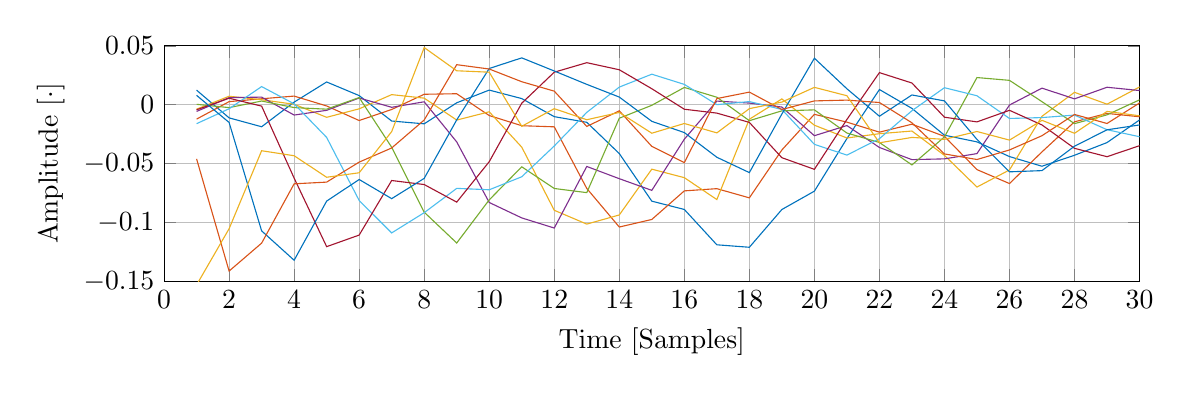
\begin{tikzpicture}

\begin{axis}[%
width=5.5in,
height=1.8in,
%scale only axis,
scaled y ticks = false,
y tick label style={/pgf/number format/fixed},
xmin=0,
xmajorgrids,
xminorgrids,
ymajorgrids,
xmax=30,
xlabel={Time [Samples]},
ymin=-0.15,
ymax=0.05,
ylabel={Amplitude [$\cdot$]},
axis background/.style={fill=white},
title style={font=\bfseries},
%title={Transfer Function from Ref to Speaker - Time domain 256 coefficients},
%legend style={legend cell align=left,align=left,draw=white!15!black}
]
\addplot [color=mycolor1,solid]
  table[row sep=crcr]{%
1	0.01233\\
2	-0.011205\\
3	-0.018745\\
4	0.0021637\\
5	0.019284\\
6	0.0077183\\
7	-0.013894\\
8	-0.016265\\
9	0.001598\\
10	0.012393\\
11	0.0051825\\
12	-0.010181\\
13	-0.014979\\
14	-0.041511\\
15	-0.081947\\
16	-0.088997\\
17	-0.11901\\
18	-0.12111\\
19	-0.089036\\
20	-0.073464\\
21	-0.028799\\
22	0.012871\\
23	-0.0031699\\
24	-0.025922\\
25	-0.031595\\
26	-0.044074\\
27	-0.052291\\
28	-0.042946\\
29	-0.032182\\
30	-0.01296\\
31	-0.0058515\\
32	0.0013563\\
33	0.018578\\
34	0.027141\\
35	0.034597\\
36	0.03384\\
37	0.019776\\
38	0.019548\\
39	0.014348\\
40	0.0065225\\
41	0.019415\\
42	0.02632\\
43	0.02164\\
44	0.020588\\
45	0.021529\\
46	0.023127\\
47	0.022136\\
48	0.011573\\
49	0.006165\\
50	0.0094142\\
51	0.0098467\\
52	0.0094966\\
53	0.0055436\\
54	-0.004496\\
55	-0.0029134\\
56	-0.0018747\\
57	-0.0082804\\
58	-0.0073456\\
59	-0.00594\\
60	-0.0077301\\
61	-0.0068324\\
62	-0.00051272\\
63	-0.0063771\\
64	-0.010733\\
65	-0.0044857\\
66	-0.0023259\\
67	-0.00096752\\
68	-0.0001599\\
69	-0.0060575\\
70	-0.0061309\\
71	0.0014948\\
72	0.0049747\\
73	0.0015052\\
74	-0.00239\\
75	-0.0004734\\
76	0.0042407\\
77	0.0052325\\
78	0.0039426\\
79	0.0043007\\
80	0.00088237\\
81	0.0047778\\
82	0.0096333\\
83	0.0039356\\
84	0.0015876\\
85	0.0031294\\
86	0.0023196\\
87	0.0059317\\
88	0.0055782\\
89	-0.00034692\\
90	-0.00080376\\
91	0.0030833\\
92	0.0071669\\
93	0.0052589\\
94	-0.00058343\\
95	-0.0019373\\
96	0.0020072\\
97	0.0024913\\
98	0.0023054\\
99	-0.0015619\\
100	-0.0062139\\
101	-0.0012558\\
102	0.0043953\\
103	0.0017503\\
104	-0.0013437\\
105	-0.0023485\\
106	-0.00086767\\
107	0.0026458\\
108	0.0037845\\
109	0.00022114\\
110	-0.0036756\\
111	-0.00034839\\
112	0.0041405\\
113	0.0040394\\
114	0.00016571\\
115	-0.0020679\\
116	-0.00023064\\
117	0.0041411\\
118	0.0053986\\
119	0.0011628\\
120	-0.0026911\\
121	0.00011243\\
122	0.0054391\\
123	0.0049004\\
124	0.00034959\\
125	-0.0008664\\
126	-0.00026219\\
127	0.002822\\
128	0.0066216\\
129	0.0015561\\
130	-0.0031978\\
131	-0.00019011\\
132	0.0041999\\
133	0.0054329\\
134	0.003011\\
135	-0.0012099\\
136	-0.00010412\\
137	0.0047904\\
138	0.0062031\\
139	0.0031034\\
140	-0.0011866\\
141	-0.0025291\\
142	0.0018334\\
143	0.0038032\\
144	0.00083764\\
145	-0.0011594\\
146	-0.0025603\\
147	0.0013417\\
148	0.0062545\\
149	0.0033724\\
150	-0.0024503\\
151	-0.001949\\
152	0.0017121\\
153	0.0028636\\
154	0.0011426\\
155	-0.0022159\\
156	-0.0034381\\
157	0.00014631\\
158	0.003766\\
159	0.0032847\\
160	-0.00082264\\
161	-0.002276\\
162	0.001252\\
163	0.0036529\\
164	0.0032008\\
165	-0.00037563\\
166	-0.0028289\\
167	0.00010239\\
168	0.0044132\\
169	0.0034075\\
170	-0.00027145\\
171	-0.0015691\\
172	-0.00017776\\
173	0.0029894\\
174	0.004744\\
175	0.00081565\\
176	-0.0023178\\
177	0.000442\\
178	0.003822\\
179	0.0040902\\
180	0.00065177\\
181	-0.0021308\\
182	-0.00063469\\
183	0.0026019\\
184	0.0032299\\
185	0.0018497\\
186	-0.00016169\\
187	-0.00017935\\
188	0.0035645\\
189	0.0050709\\
190	0.0016094\\
191	-0.0011678\\
192	-0.0018781\\
193	0.00063209\\
194	0.0035994\\
195	0.0014847\\
196	-0.00098023\\
197	0.00058198\\
198	0.0033014\\
199	0.0042651\\
200	0.0030949\\
201	3.3513e-05\\
202	-0.0012025\\
203	0.00077499\\
204	0.0024118\\
205	0.0018712\\
206	-0.00028506\\
207	-0.00098012\\
208	0.001596\\
209	0.0036706\\
210	0.0033768\\
211	0.0013463\\
212	-0.00079262\\
213	0.000616\\
214	0.0030916\\
215	0.0022143\\
216	-0.00051118\\
217	-0.00071363\\
218	0.0009213\\
219	0.0025515\\
220	0.0028505\\
221	0.0011539\\
222	-0.00010293\\
223	0.0013708\\
224	0.0024841\\
225	0.0021055\\
226	0.00096385\\
227	-0.00016105\\
228	-0.00011888\\
229	0.0021282\\
230	0.0038479\\
231	0.0013238\\
232	-0.0013443\\
233	-0.00039601\\
234	0.0015058\\
235	0.001694\\
236	0.0012445\\
237	-0.00026766\\
238	-0.0016419\\
239	0.00025531\\
240	0.0024616\\
241	0.00069813\\
242	-0.00078334\\
243	-0.00016042\\
244	0.0004221\\
245	0.0012738\\
246	0.0012546\\
247	-0.00062945\\
248	-0.0010677\\
249	0.0002752\\
250	0.0007981\\
251	0.0011216\\
252	0.00076865\\
253	0.00071331\\
254	0.0026205\\
255	0.0039567\\
256	0.0024428\\
};
%\addlegendentry{0};

\addplot [color=mycolor2,solid]
  table[row sep=crcr]{%
1	-0.012253\\
2	0.0025874\\
3	0.0050144\\
4	0.0072989\\
5	-0.0010881\\
6	-0.013464\\
7	-0.0040854\\
8	0.0088468\\
9	0.0093018\\
10	-0.0092389\\
11	-0.017858\\
12	-0.01881\\
13	-0.071145\\
14	-0.10392\\
15	-0.097489\\
16	-0.073212\\
17	-0.071331\\
18	-0.079136\\
19	-0.038472\\
20	-0.0081998\\
21	-0.014823\\
22	-0.02333\\
23	-0.016584\\
24	-0.026912\\
25	-0.055145\\
26	-0.06699\\
27	-0.04008\\
28	-0.014547\\
29	-0.0074133\\
30	-0.010255\\
31	0.016899\\
32	0.032549\\
33	0.019272\\
34	0.013254\\
35	0.020424\\
36	0.021683\\
37	0.0067138\\
38	-0.0093819\\
39	-0.001242\\
40	0.017942\\
41	0.02268\\
42	0.021013\\
43	0.028228\\
44	0.028297\\
45	0.020952\\
46	0.010458\\
47	0.0044913\\
48	0.018521\\
49	0.012339\\
50	-0.0043116\\
51	0.0024022\\
52	0.0070417\\
53	-0.00080072\\
54	-0.0042539\\
55	-0.00032604\\
56	0.0029769\\
57	0.0013801\\
58	-0.0068828\\
59	-0.013557\\
60	-0.0045915\\
61	-0.0017303\\
62	-0.005109\\
63	-0.0066769\\
64	-0.0052432\\
65	0.0025106\\
66	-0.0015767\\
67	-0.0075386\\
68	0.003074\\
69	0.00444\\
70	-5.3916e-06\\
71	0.001411\\
72	3.5634e-05\\
73	0.00018691\\
74	0.0046878\\
75	-0.00068633\\
76	-0.00052774\\
77	0.010247\\
78	0.0035224\\
79	-0.0019677\\
80	0.0053782\\
81	0.0064136\\
82	0.0045604\\
83	9.2224e-05\\
84	-0.00015378\\
85	0.0067658\\
86	0.0034035\\
87	-0.0021759\\
88	0.0012042\\
89	0.0043493\\
90	0.0050201\\
91	0.005042\\
92	-0.0021207\\
93	0.00095045\\
94	0.0084776\\
95	-0.0027632\\
96	-0.0042545\\
97	0.0051014\\
98	-0.00090345\\
99	-0.002078\\
100	0.0013316\\
101	-0.00062834\\
102	0.0017973\\
103	0.0012203\\
104	-0.0026746\\
105	0.0018873\\
106	0.0025761\\
107	-0.0026369\\
108	-0.0010561\\
109	0.00034684\\
110	0.0026678\\
111	0.0030563\\
112	-0.0042352\\
113	0.0021051\\
114	0.0074967\\
115	-0.0027178\\
116	-0.00043824\\
117	0.0041058\\
118	-0.0010477\\
119	0.0028283\\
120	0.0038005\\
121	-0.0038547\\
122	0.0033521\\
123	0.0069338\\
124	-0.0019264\\
125	0.0021425\\
126	0.0044136\\
127	2.5273e-05\\
128	0.0030277\\
129	0.0018344\\
130	0.0023592\\
131	0.0038595\\
132	-1.1115e-05\\
133	0.0038202\\
134	0.0041241\\
135	-0.0010418\\
136	0.0017749\\
137	0.001696\\
138	-0.0014859\\
139	0.0039382\\
140	0.0021989\\
141	-0.0041357\\
142	0.004296\\
143	0.0046888\\
144	-0.00284\\
145	0.0016451\\
146	0.00048499\\
147	-0.0013608\\
148	0.0032446\\
149	-0.0010518\\
150	-0.002101\\
151	0.0018276\\
152	0.0012147\\
153	0.0018376\\
154	0.00095658\\
155	-0.00097498\\
156	0.0030358\\
157	0.00081008\\
158	-0.0024819\\
159	0.004001\\
160	0.00060901\\
161	-0.0029911\\
162	0.005206\\
163	0.0017025\\
164	-0.0016713\\
165	0.0039309\\
166	0.0004472\\
167	0.00061102\\
168	0.0050052\\
169	-0.00067956\\
170	-0.0023251\\
171	0.003292\\
172	0.0023101\\
173	0.00072431\\
174	-3.7373e-05\\
175	-0.00055538\\
176	0.0040239\\
177	0.0015462\\
178	-0.0017105\\
179	0.0029091\\
180	-0.00038404\\
181	-0.00019568\\
182	0.0047017\\
183	-0.0012435\\
184	-0.00042077\\
185	0.0052854\\
186	-4.5661e-05\\
187	0.00042335\\
188	0.0044776\\
189	-0.0017248\\
190	-0.0010264\\
191	0.0044064\\
192	0.00070453\\
193	0.00014714\\
194	0.0011353\\
195	0.00088537\\
196	0.0042537\\
197	0.0021312\\
198	0.00036481\\
199	0.002237\\
200	1.9725e-05\\
201	0.00183\\
202	0.0024676\\
203	-0.0031987\\
204	0.0011749\\
205	0.0061782\\
206	-0.00052596\\
207	0.00061081\\
208	0.0042955\\
209	-0.00022173\\
210	0.0028654\\
211	0.0039292\\
212	-0.0017291\\
213	0.00072423\\
214	0.0011899\\
215	-0.00051764\\
216	0.0029857\\
217	0.0017848\\
218	-0.00019336\\
219	0.0017055\\
220	0.0020218\\
221	0.0030461\\
222	0.0013417\\
223	-0.0027736\\
224	0.0029312\\
225	0.0049486\\
226	-0.0028863\\
227	-0.00080569\\
228	0.00266\\
229	0.00077167\\
230	0.0036479\\
231	0.00044746\\
232	-0.0030338\\
233	0.0031644\\
234	0.002507\\
235	-0.0020063\\
236	0.0010059\\
237	0.00049917\\
238	-0.00095637\\
239	0.0016219\\
240	0.00010927\\
241	-8.5348e-05\\
242	0.0012353\\
243	-0.00075628\\
244	0.0017404\\
245	0.0018291\\
246	-0.0022362\\
247	6.6233e-05\\
248	0.0014268\\
249	0.0015363\\
250	0.0033602\\
251	-0.0007457\\
252	-0.00097736\\
253	0.006202\\
254	0.0033791\\
255	-0.0022213\\
256	0.0014502\\
};
%\addlegendentry{10};

\addplot [color=mycolor3,solid]
  table[row sep=crcr]{%
1	-0.003798\\
2	0.0071576\\
3	0.0041978\\
4	0.00034775\\
5	-0.01073\\
6	-0.0035185\\
7	0.0085377\\
8	0.0055656\\
9	-0.013074\\
10	-0.0060418\\
11	-0.036068\\
12	-0.089689\\
13	-0.10143\\
14	-0.093667\\
15	-0.05477\\
16	-0.061992\\
17	-0.080572\\
18	-0.01237\\
19	0.004902\\
20	-0.017438\\
21	-0.028285\\
22	-0.024652\\
23	-0.022378\\
24	-0.04303\\
25	-0.06996\\
26	-0.055422\\
27	-0.0098306\\
28	0.010515\\
29	0.00042614\\
30	0.015041\\
31	0.016444\\
32	0.017783\\
33	0.016517\\
34	0.0061112\\
35	0.0081121\\
36	-0.0023927\\
37	-0.010656\\
38	0.0065508\\
39	0.010754\\
40	0.013093\\
41	0.014412\\
42	0.02645\\
43	0.040257\\
44	0.012454\\
45	-0.0086203\\
46	0.011909\\
47	0.022317\\
48	0.014732\\
49	-0.0041516\\
50	-0.0069798\\
51	0.0091946\\
52	0.016715\\
53	-0.0073573\\
54	-0.011609\\
55	0.010277\\
56	0.010083\\
57	-0.0060943\\
58	-0.017165\\
59	-0.011174\\
60	0.0082134\\
61	-0.00046486\\
62	-0.0088348\\
63	-0.0034489\\
64	-0.0024103\\
65	0.000609\\
66	-5.887e-05\\
67	0.00088066\\
68	0.0065453\\
69	-0.00096964\\
70	-0.0028653\\
71	0.0058705\\
72	0.0031886\\
73	-0.0065395\\
74	0.0024119\\
75	0.010233\\
76	0.0070393\\
77	-0.0012654\\
78	-0.0087956\\
79	0.0075056\\
80	0.019175\\
81	-0.0023308\\
82	-0.009669\\
83	0.0017264\\
84	0.010268\\
85	0.0052848\\
86	-0.0095582\\
87	-0.0015379\\
88	0.014942\\
89	0.008054\\
90	-0.0041393\\
91	-0.0050111\\
92	0.0050696\\
93	0.0097051\\
94	-0.00015024\\
95	-0.0068164\\
96	0.0017673\\
97	0.0031422\\
98	-0.0023367\\
99	0.001639\\
100	0.001738\\
101	-0.00077454\\
102	0.0020166\\
103	-0.0016292\\
104	0.0019766\\
105	0.00046284\\
106	-0.0068132\\
107	0.0028095\\
108	0.0081112\\
109	-0.0011722\\
110	-0.0057435\\
111	-0.0020342\\
112	0.0087635\\
113	0.0070811\\
114	-0.0066282\\
115	-0.005383\\
116	0.0074676\\
117	0.0071895\\
118	-0.0021707\\
119	-0.0065203\\
120	0.0029575\\
121	0.013207\\
122	0.0022886\\
123	-0.0081562\\
124	0.0031187\\
125	0.008912\\
126	0.0047288\\
127	0.0004334\\
128	-0.0019324\\
129	0.005284\\
130	0.005547\\
131	-0.002541\\
132	0.00062768\\
133	0.003237\\
134	2.1744e-05\\
135	0.00061465\\
136	0.0033707\\
137	0.0017764\\
138	-0.00069751\\
139	-5.0556e-05\\
140	0.0056019\\
141	0.0046092\\
142	-0.0038847\\
143	-0.0055773\\
144	0.0025087\\
145	0.004724\\
146	0.00086359\\
147	-0.0068757\\
148	-6.5211e-05\\
149	0.011113\\
150	0.001465\\
151	-0.0065329\\
152	0.00089677\\
153	0.005369\\
154	0.0050641\\
155	-0.0034094\\
156	-0.0065801\\
157	0.0041338\\
158	0.0073641\\
159	-0.0010246\\
160	-0.0024793\\
161	0.0031933\\
162	0.004072\\
163	0.0013595\\
164	-7.8527e-05\\
165	0.00086209\\
166	0.0029957\\
167	0.00068555\\
168	0.00045713\\
169	0.0015353\\
170	0.0001734\\
171	0.0003925\\
172	0.00075846\\
173	0.003308\\
174	0.0034409\\
175	-0.0048111\\
176	-0.00038849\\
177	0.0069583\\
178	0.0017845\\
179	-0.0036131\\
180	-0.00136\\
181	0.0028975\\
182	0.0058115\\
183	-0.00057588\\
184	-0.004534\\
185	0.0034413\\
186	0.0085564\\
187	-0.0009004\\
188	-0.004652\\
189	0.0010305\\
190	0.0055719\\
191	0.002985\\
192	-0.0025987\\
193	-0.00015776\\
194	0.0045615\\
195	0.0036341\\
196	0.00086389\\
197	-0.00058158\\
198	0.002389\\
199	0.0036183\\
200	-0.0022209\\
201	0.00024777\\
202	0.0029668\\
203	0.00055479\\
204	0.0010884\\
205	0.0044621\\
206	0.0018748\\
207	0.0012652\\
208	0.00093932\\
209	0.0020764\\
210	0.0049024\\
211	0.0015334\\
212	-0.0057349\\
213	0.0010684\\
214	0.0066428\\
215	0.0020019\\
216	-0.003145\\
217	4.9462e-05\\
218	0.0060971\\
219	0.0044576\\
220	-0.0031556\\
221	-0.0022814\\
222	0.0035239\\
223	0.0064534\\
224	-0.0012173\\
225	-0.0059003\\
226	0.0018805\\
227	0.0076543\\
228	0.00052108\\
229	-0.0031744\\
230	0.00070247\\
231	0.003845\\
232	0.0013446\\
233	-0.0015497\\
234	-0.001839\\
235	0.0031142\\
236	0.0016615\\
237	-0.0016753\\
238	0.00034471\\
239	0.001203\\
240	-0.00093316\\
241	0.0013307\\
242	0.0023195\\
243	0.001285\\
244	-0.0024005\\
245	-0.0010334\\
246	0.0035428\\
247	0.0042754\\
248	0.00019092\\
249	-0.0021348\\
250	0.0015933\\
251	0.0069972\\
252	0.0013466\\
253	-0.0037716\\
254	0.00087312\\
255	0.0059432\\
256	0.0035049\\
};
%\addlegendentry{20};

\addplot [color=mycolor4,solid]
  table[row sep=crcr]{%
1	-0.0057158\\
2	0.006003\\
3	0.0064072\\
4	-0.0088078\\
5	-0.0047986\\
6	0.0056824\\
7	-0.0022257\\
8	0.0024547\\
9	-0.03162\\
10	-0.083079\\
11	-0.096175\\
12	-0.10477\\
13	-0.052483\\
14	-0.062854\\
15	-0.072782\\
16	-0.029323\\
17	0.0030557\\
18	0.0013594\\
19	-0.002015\\
20	-0.026352\\
21	-0.017734\\
22	-0.036346\\
23	-0.046682\\
24	-0.046022\\
25	-0.041557\\
26	-0.00030949\\
27	0.014057\\
28	0.0049482\\
29	0.014799\\
30	0.012006\\
31	-0.0033943\\
32	0.0035565\\
33	0.0058034\\
34	-0.0030174\\
35	-0.017892\\
36	-0.0053392\\
37	0.0021074\\
38	0.0020354\\
39	0.016183\\
40	0.01206\\
41	0.012895\\
42	0.013916\\
43	0.015656\\
44	0.011967\\
45	0.012146\\
46	0.007938\\
47	0.0047777\\
48	0.0058956\\
49	0.014486\\
50	0.0007137\\
51	-0.0047032\\
52	0.0095627\\
53	0.0088159\\
54	0.005612\\
55	-0.0085075\\
56	-7.2957e-05\\
57	-0.0027086\\
58	-0.0033396\\
59	-0.0051093\\
60	-0.0041445\\
61	-0.0081334\\
62	0.0077991\\
63	-0.0091863\\
64	0.0046493\\
65	0.0050492\\
66	-4.715e-05\\
67	-0.0015986\\
68	0.001576\\
69	0.0035343\\
70	0.0017726\\
71	-0.0049491\\
72	0.0060764\\
73	0.0059967\\
74	-0.00067676\\
75	0.0047088\\
76	-0.0011988\\
77	0.0093981\\
78	0.00070289\\
79	-0.00056719\\
80	0.0015185\\
81	0.0037979\\
82	-0.0024079\\
83	0.0011069\\
84	0.00088504\\
85	0.0092923\\
86	-0.0019328\\
87	-0.00022461\\
88	0.0058737\\
89	0.0043548\\
90	0.0024638\\
91	-0.0026433\\
92	0.0018612\\
93	0.0048007\\
94	-0.0015497\\
95	-0.0034641\\
96	0.0038833\\
97	0.0021489\\
98	0.00019914\\
99	-0.0041206\\
100	0.0039944\\
101	0.0011568\\
102	-0.0024509\\
103	-0.00052407\\
104	1.2673e-05\\
105	0.0038928\\
106	-0.001586\\
107	-0.0030918\\
108	0.0023982\\
109	0.0042249\\
110	-0.0024502\\
111	-0.0012502\\
112	0.00091095\\
113	0.0071488\\
114	-0.0055163\\
115	0.0010995\\
116	0.0045325\\
117	0.0017534\\
118	0.00026505\\
119	0.0022515\\
120	0.0047272\\
121	0.00609\\
122	0.00027418\\
123	0.002242\\
124	0.0043187\\
125	0.0029642\\
126	0.0013437\\
127	-0.0064493\\
128	0.0072639\\
129	0.0025115\\
130	-0.0032853\\
131	0.00028008\\
132	0.0060348\\
133	0.0014343\\
134	0.001422\\
135	-0.0015897\\
136	0.006183\\
137	-0.0018448\\
138	-0.0014639\\
139	0.00032784\\
140	-0.00039894\\
141	0.0035104\\
142	-0.0019332\\
143	-0.0020267\\
144	0.0060694\\
145	0.0028384\\
146	-0.0032128\\
147	0.0016166\\
148	0.0033672\\
149	0.0034329\\
150	-0.0053936\\
151	0.0028733\\
152	0.0032502\\
153	-0.00064869\\
154	-0.00024621\\
155	0.0010439\\
156	0.0027835\\
157	0.0031888\\
158	-0.0019972\\
159	0.0010043\\
160	0.0042366\\
161	0.0022133\\
162	-0.0012061\\
163	-0.0015023\\
164	0.0072112\\
165	-0.00061598\\
166	-0.0027907\\
167	0.0022144\\
168	0.0032798\\
169	3.3269e-05\\
170	-0.00048715\\
171	0.0011201\\
172	0.0038186\\
173	-0.0006161\\
174	-5.1804e-05\\
175	0.00068439\\
176	0.0015137\\
177	0.0026864\\
178	-0.0046664\\
179	0.0023\\
180	0.0046054\\
181	0.00019691\\
182	-0.0014314\\
183	0.0030913\\
184	0.0030782\\
185	0.0008901\\
186	-0.0036874\\
187	0.0047638\\
188	0.0012811\\
189	6.2204e-07\\
190	0.001464\\
191	0.0010837\\
192	0.0045949\\
193	0.0009631\\
194	-0.0015516\\
195	0.0032593\\
196	0.0028301\\
197	-0.001333\\
198	-0.00057276\\
199	0.0011078\\
200	0.0058752\\
201	-0.0026824\\
202	0.001677\\
203	0.0046458\\
204	0.0028515\\
205	0.00017227\\
206	0.0013284\\
207	0.0028163\\
208	0.0035865\\
209	-0.0023773\\
210	0.00075568\\
211	0.003138\\
212	0.0023141\\
213	9.7267e-05\\
214	-0.00074123\\
215	0.0050406\\
216	0.0012961\\
217	-0.0021423\\
218	0.00090034\\
219	0.0036464\\
220	0.001253\\
221	-0.0012872\\
222	-0.0011973\\
223	0.0039414\\
224	0.0014335\\
225	-0.00037131\\
226	0.00036525\\
227	0.002115\\
228	0.0025034\\
229	-0.0032642\\
230	0.00064926\\
231	0.0039544\\
232	-0.00040367\\
233	-0.0022738\\
234	0.0017428\\
235	0.0021378\\
236	0.00043881\\
237	-0.0032635\\
238	0.0029153\\
239	0.0023263\\
240	-0.00016825\\
241	-0.00031897\\
242	-0.00078429\\
243	0.0048191\\
244	0.0031747\\
245	-0.0026833\\
246	0.0013445\\
247	0.0035938\\
248	0.0011928\\
249	-7.6708e-05\\
250	-0.0004657\\
251	0.0058943\\
252	8.7292e-05\\
253	-0.00018379\\
254	0.004192\\
255	0.0014655\\
256	0.00073253\\
};
%\addlegendentry{30};

\addplot [color=mycolor5,solid]
  table[row sep=crcr]{%
1	0.00029868\\
2	-0.0024872\\
3	0.0030811\\
4	-0.0024722\\
5	-0.0038139\\
6	0.0060497\\
7	-0.036152\\
8	-0.091305\\
9	-0.11749\\
10	-0.080854\\
11	-0.052772\\
12	-0.071184\\
13	-0.074702\\
14	-0.011505\\
15	-0.00052293\\
16	0.014649\\
17	0.006324\\
18	-0.013595\\
19	-0.0052387\\
20	-0.0044231\\
21	-0.024067\\
22	-0.032106\\
23	-0.051172\\
24	-0.027388\\
25	0.02304\\
26	0.020667\\
27	0.0025547\\
28	-0.016093\\
29	-0.0086353\\
30	0.0041154\\
31	-0.0013129\\
32	-0.03232\\
33	-0.015467\\
34	-0.010234\\
35	-6.3968e-05\\
36	-0.010003\\
37	-0.0090942\\
38	0.0043213\\
39	0.022702\\
40	0.021448\\
41	0.019155\\
42	0.0018637\\
43	-0.0054651\\
44	0.015479\\
45	0.017577\\
46	0.016548\\
47	0.0017911\\
48	0.0036623\\
49	0.014971\\
50	0.019785\\
51	0.00021908\\
52	0.00043067\\
53	-0.0013598\\
54	0.0058793\\
55	0.00045561\\
56	-0.01359\\
57	-0.013351\\
58	-0.0012345\\
59	0.0025111\\
60	0.0045389\\
61	-0.00076914\\
62	-0.0068689\\
63	0.0037005\\
64	0.0042929\\
65	0.0058253\\
66	-0.0020652\\
67	-0.0052466\\
68	0.00050259\\
69	0.0098141\\
70	0.0030698\\
71	0.0019\\
72	-0.0010339\\
73	0.0057666\\
74	0.011151\\
75	0.0016729\\
76	-0.0016667\\
77	-0.00037291\\
78	0.0033339\\
79	0.0040238\\
80	0.0015258\\
81	-0.0066416\\
82	0.0035612\\
83	0.0034184\\
84	0.0070312\\
85	0.002464\\
86	-0.00083144\\
87	-0.00028105\\
88	0.0056339\\
89	0.0027145\\
90	0.00097073\\
91	-0.0025618\\
92	-0.0013299\\
93	0.0062108\\
94	0.00081435\\
95	0.00016166\\
96	-0.0020047\\
97	0.0016742\\
98	0.0027927\\
99	0.0037384\\
100	-0.0060224\\
101	0.00015643\\
102	-0.00054735\\
103	0.0044737\\
104	0.00070743\\
105	-0.0009376\\
106	-0.0027059\\
107	0.0027355\\
108	0.0009718\\
109	0.0019881\\
110	-0.00064\\
111	-0.00055562\\
112	0.0047548\\
113	0.0036133\\
114	0.0028755\\
115	0.0017135\\
116	0.002516\\
117	0.0028401\\
118	0.0058293\\
119	-0.0011839\\
120	0.00032695\\
121	-0.0010325\\
122	0.0025925\\
123	0.0020089\\
124	0.0014659\\
125	-0.00090024\\
126	0.0035432\\
127	0.002084\\
128	0.0037027\\
129	0.0013325\\
130	-0.00031183\\
131	0.0019244\\
132	0.0022038\\
133	-0.00051005\\
134	0.0014593\\
135	-0.00071\\
136	0.0007464\\
137	0.0034619\\
138	0.0016912\\
139	0.00019595\\
140	0.001668\\
141	0.00019827\\
142	0.0032736\\
143	0.0011191\\
144	-0.00042119\\
145	0.00035902\\
146	0.0012203\\
147	0.00083037\\
148	0.0020411\\
149	-0.00069703\\
150	0.0014621\\
151	0.0028075\\
152	0.00026622\\
153	0.0025707\\
154	6.6836e-05\\
155	0.0012916\\
156	0.0017175\\
157	0.0030257\\
158	-0.00077222\\
159	0.0031339\\
160	-0.0014768\\
161	0.0039459\\
162	0.00040437\\
163	0.002215\\
164	-0.0011523\\
165	0.0033063\\
166	-0.00042969\\
167	0.0040907\\
168	-0.0021851\\
169	0.0019893\\
170	0.0007708\\
171	0.0013483\\
172	0.00092888\\
173	0.001301\\
174	-0.00067\\
175	0.0014249\\
176	0.0023133\\
177	-0.00071098\\
178	0.0029445\\
179	-0.00085421\\
180	0.0027015\\
181	9.0931e-05\\
182	0.0027517\\
183	-0.0017537\\
184	0.0036714\\
185	-0.0011379\\
186	0.0052241\\
187	-0.0014254\\
188	0.0033013\\
189	-1.1707e-05\\
190	0.0026909\\
191	-0.00032377\\
192	0.0032619\\
193	-0.0012689\\
194	0.0024969\\
195	0.0013365\\
196	0.00066383\\
197	0.0016533\\
198	0.0019183\\
199	0.0025548\\
200	0.0022132\\
201	0.0031728\\
202	0.00069515\\
203	0.0029281\\
204	-0.00052497\\
205	0.0043435\\
206	-0.00073476\\
207	0.003007\\
208	-5.4531e-05\\
209	0.0027827\\
210	-0.00081076\\
211	0.0039043\\
212	-0.0016325\\
213	0.002874\\
214	-0.00017513\\
215	0.0013506\\
216	-0.00024422\\
217	0.0027231\\
218	-0.00042345\\
219	0.00064893\\
220	0.00049811\\
221	0.0027808\\
222	0.0014084\\
223	-0.00075541\\
224	0.0023146\\
225	0.00038728\\
226	0.0010959\\
227	0.00025626\\
228	0.0017219\\
229	-0.0013396\\
230	0.0030319\\
231	-0.00074901\\
232	0.0012833\\
233	-0.001592\\
234	0.0016097\\
235	0.00016951\\
236	0.0027484\\
237	0.00022873\\
238	0.003233\\
239	-6.5365e-05\\
240	0.0027328\\
241	0.00062825\\
242	0.0014083\\
243	0.00081986\\
244	0.00083704\\
245	0.00047915\\
246	0.0020838\\
247	0.001693\\
248	0.0016807\\
249	0.0023743\\
250	0.00037931\\
251	0.0030219\\
252	0.00035257\\
253	0.0010541\\
254	-0.00068867\\
255	0.00087367\\
256	-0.00035914\\
};
%\addlegendentry{40};

\addplot [color=mycolor6,solid]
  table[row sep=crcr]{%
1	-0.01614\\
2	-0.0034697\\
3	0.015382\\
4	0.00070632\\
5	-0.02782\\
6	-0.081384\\
7	-0.10891\\
8	-0.091732\\
9	-0.071086\\
10	-0.072279\\
11	-0.061231\\
12	-0.035093\\
13	-0.0065342\\
14	0.014928\\
15	0.025898\\
16	0.017232\\
17	2.0598e-05\\
18	0.0026337\\
19	-0.0040449\\
20	-0.033694\\
21	-0.042826\\
22	-0.028875\\
23	-0.0051464\\
24	0.014422\\
25	0.0075707\\
26	-0.011711\\
27	-0.010955\\
28	-0.0088396\\
29	-0.021272\\
30	-0.027216\\
31	-0.018363\\
32	-0.016832\\
33	-0.023388\\
34	-0.016311\\
35	-0.00090588\\
36	0.0059122\\
37	0.01564\\
38	0.020887\\
39	0.01439\\
40	0.0096355\\
41	0.00067997\\
42	0.0018199\\
43	0.014988\\
44	0.020351\\
45	0.0077674\\
46	0.0074161\\
47	0.018457\\
48	0.013282\\
49	0.0014066\\
50	0.0058043\\
51	0.008308\\
52	-0.003361\\
53	-0.01136\\
54	-0.0077384\\
55	-0.0067202\\
56	-0.0026441\\
57	0.00070902\\
58	0.0022464\\
59	0.0066327\\
60	0.0019008\\
61	-0.0041521\\
62	9.1799e-05\\
63	0.0091305\\
64	-0.0015922\\
65	-0.008618\\
66	0.0025676\\
67	0.0079476\\
68	-0.00090487\\
69	0.0017744\\
70	0.01104\\
71	0.0079605\\
72	0.00093401\\
73	0.0021056\\
74	0.0022464\\
75	0.0032024\\
76	-0.00045155\\
77	-0.0030124\\
78	0.001513\\
79	0.003992\\
80	-0.0012762\\
81	-0.0020608\\
82	0.010235\\
83	0.0066527\\
84	-0.0039971\\
85	-0.00082811\\
86	0.0074804\\
87	9.7903e-05\\
88	-0.0038645\\
89	0.0021608\\
90	0.0041231\\
91	0.00024156\\
92	-0.00051648\\
93	0.00022795\\
94	0.0046167\\
95	0.0027802\\
96	-0.0019663\\
97	-0.0019146\\
98	0.0038938\\
99	-2.1487e-05\\
100	-0.0070374\\
101	0.0024604\\
102	0.0065501\\
103	-0.0020567\\
104	-0.0044201\\
105	0.005957\\
106	0.0046193\\
107	-0.00083959\\
108	0.00065823\\
109	0.0048149\\
110	0.0026963\\
111	-0.0003381\\
112	-0.0019768\\
113	0.0021781\\
114	0.0037713\\
115	0.00065473\\
116	-0.0031739\\
117	0.0042559\\
118	0.0047403\\
119	-0.0037693\\
120	-0.00033777\\
121	0.0074542\\
122	0.0030949\\
123	-0.0037215\\
124	0.0028542\\
125	0.0052546\\
126	0.0016699\\
127	-0.00057367\\
128	0.0034655\\
129	0.0037405\\
130	0.0016622\\
131	-0.0019274\\
132	-0.00063908\\
133	0.0027093\\
134	0.0026132\\
135	-0.0041402\\
136	0.0013736\\
137	0.0055553\\
138	-0.00084673\\
139	-0.0036466\\
140	0.0040509\\
141	0.0048471\\
142	-0.0022015\\
143	-0.0011701\\
144	0.0026069\\
145	0.002274\\
146	-0.0014356\\
147	0.00085188\\
148	0.0025344\\
149	0.0037069\\
150	0.00096334\\
151	-0.0003974\\
152	0.0026109\\
153	0.0057023\\
154	-0.0022163\\
155	-0.00099926\\
156	0.0043452\\
157	0.0028019\\
158	-0.0035425\\
159	0.00054604\\
160	0.0045416\\
161	0.0014168\\
162	-0.0015253\\
163	0.0014284\\
164	0.0033116\\
165	0.00057704\\
166	7.732e-05\\
167	-0.00015884\\
168	0.002478\\
169	0.0024247\\
170	-0.0014369\\
171	-0.00086347\\
172	0.005296\\
173	0.00065023\\
174	-0.0019803\\
175	0.0012075\\
176	0.0046705\\
177	-0.00067553\\
178	-0.0013624\\
179	0.0019527\\
180	0.003462\\
181	-0.00049826\\
182	-4.4359e-05\\
183	0.0018325\\
184	0.0025636\\
185	0.0020613\\
186	-0.00096288\\
187	0.00042205\\
188	0.0044128\\
189	0.00091326\\
190	-0.0023651\\
191	0.0031223\\
192	0.0035583\\
193	0.00023756\\
194	-0.0011597\\
195	0.0041469\\
196	0.0035469\\
197	0.001067\\
198	0.00055873\\
199	0.0039492\\
200	0.0017826\\
201	0.00073795\\
202	-0.0007565\\
203	0.0021225\\
204	0.0042741\\
205	0.00029558\\
206	-0.0029283\\
207	0.0032912\\
208	0.0033596\\
209	-0.0013711\\
210	-0.0010171\\
211	0.0033753\\
212	0.0025479\\
213	-0.0020791\\
214	0.00027407\\
215	0.0032381\\
216	0.0012534\\
217	-0.001284\\
218	0.0018291\\
219	0.0025227\\
220	0.0021261\\
221	-0.0016484\\
222	-0.0008872\\
223	0.0035563\\
224	0.0026192\\
225	-0.0030429\\
226	-0.00017057\\
227	0.0036854\\
228	0.0015174\\
229	-0.0037664\\
230	-5.7789e-05\\
231	0.0041835\\
232	0.00098605\\
233	-0.00020691\\
234	0.0030985\\
235	0.0030624\\
236	-0.00010857\\
237	0.0011225\\
238	0.001831\\
239	0.002993\\
240	-0.00043174\\
241	-0.0020703\\
242	0.0016645\\
243	0.0051097\\
244	-0.00025212\\
245	-0.0018941\\
246	0.0030157\\
247	0.006083\\
248	-0.0017238\\
249	-0.0025401\\
250	0.0018279\\
251	0.0010143\\
252	-0.0022584\\
253	0.00065662\\
254	0.0027776\\
255	0.0014484\\
256	0.00075221\\
};
%\addlegendentry{50};

\addplot [color=mycolor7,solid]
  table[row sep=crcr]{%
1	-0.0043531\\
2	0.0054733\\
3	-0.0012234\\
4	-0.062372\\
5	-0.12059\\
6	-0.11075\\
7	-0.064411\\
8	-0.067831\\
9	-0.082754\\
10	-0.04843\\
11	0.0012435\\
12	0.027583\\
13	0.035675\\
14	0.029658\\
15	0.013545\\
16	-0.0038651\\
17	-0.0071636\\
18	-0.015054\\
19	-0.045034\\
20	-0.05491\\
21	-0.01257\\
22	0.027226\\
23	0.018402\\
24	-0.010638\\
25	-0.01462\\
26	-0.0047788\\
27	-0.017226\\
28	-0.037083\\
29	-0.044176\\
30	-0.034834\\
31	-0.025157\\
32	-0.012306\\
33	0.00087149\\
34	0.0077994\\
35	0.011835\\
36	0.022451\\
37	0.026761\\
38	0.009052\\
39	-0.011922\\
40	-0.0065586\\
41	0.012715\\
42	0.014696\\
43	0.0050353\\
44	0.0077688\\
45	0.019219\\
46	0.021419\\
47	0.012875\\
48	0.0042604\\
49	-0.0011421\\
50	-0.0057308\\
51	-0.0056689\\
52	-0.0043727\\
53	-0.0071188\\
54	-0.0072339\\
55	0.003153\\
56	0.014079\\
57	0.0093635\\
58	-0.0031272\\
59	-0.0039952\\
60	0.0036366\\
61	0.0023187\\
62	-0.0053544\\
63	-0.0066038\\
64	-0.0008345\\
65	0.0050656\\
66	0.0070071\\
67	0.0072924\\
68	0.0058722\\
69	0.0039472\\
70	0.0047713\\
71	0.0052667\\
72	0.00057529\\
73	-0.0050239\\
74	-0.002043\\
75	0.0053\\
76	0.0049362\\
77	-0.00034525\\
78	0.00097421\\
79	0.0059142\\
80	0.0057397\\
81	0.001973\\
82	-0.00043555\\
83	-0.00071003\\
84	0.000366\\
85	0.0013699\\
86	0.0017491\\
87	0.00083588\\
88	-0.0001098\\
89	0.0016524\\
90	0.0046002\\
91	0.0024343\\
92	-0.0020929\\
93	-0.0012303\\
94	0.0022986\\
95	0.0010631\\
96	-0.0022138\\
97	-0.00075926\\
98	0.0026514\\
99	0.0033191\\
100	0.0035139\\
101	0.0030782\\
102	0.0011945\\
103	-0.00067376\\
104	-0.00044438\\
105	0.00084674\\
106	-0.00014042\\
107	-0.0027482\\
108	-0.0010609\\
109	0.0033181\\
110	0.0035006\\
111	0.0017604\\
112	0.0028808\\
113	0.0041192\\
114	0.0015822\\
115	-0.00068815\\
116	0.00050215\\
117	0.00052419\\
118	7.4659e-05\\
119	0.0021752\\
120	0.004729\\
121	0.0046647\\
122	0.003156\\
123	0.0028961\\
124	0.0039624\\
125	0.0021036\\
126	-0.0018215\\
127	-0.0021205\\
128	-0.00076239\\
129	-0.0013742\\
130	-0.0017315\\
131	0.00086561\\
132	0.0031224\\
133	0.001938\\
134	0.0019244\\
135	0.0028438\\
136	0.001389\\
137	-0.00036845\\
138	-0.00021388\\
139	0.00067785\\
140	0.00072262\\
141	9.7727e-05\\
142	0.0010593\\
143	0.003986\\
144	0.0039864\\
145	0.0023245\\
146	0.0022418\\
147	0.00263\\
148	0.00099685\\
149	-0.00050373\\
150	0.00050676\\
151	0.00089092\\
152	-0.0001027\\
153	0.0013612\\
154	0.0024452\\
155	0.0020176\\
156	0.0010262\\
157	0.0011009\\
158	0.001598\\
159	0.0017959\\
160	-0.0002764\\
161	-0.00045522\\
162	0.00121\\
163	0.0016712\\
164	0.0011091\\
165	0.0017195\\
166	0.0022905\\
167	0.00128\\
168	0.00071321\\
169	0.0017238\\
170	0.00073217\\
171	-0.0001359\\
172	0.0006429\\
173	0.0012772\\
174	0.0012848\\
175	0.00090836\\
176	0.00081234\\
177	0.0016709\\
178	0.0021594\\
179	0.00044778\\
180	0.00048093\\
181	0.00095117\\
182	0.0013218\\
183	0.00065729\\
184	0.001574\\
185	0.0022165\\
186	0.0017595\\
187	0.0013963\\
188	0.002441\\
189	0.0016033\\
190	0.0010989\\
191	0.0007337\\
192	0.0015925\\
193	0.0020267\\
194	0.002155\\
195	0.001146\\
196	0.0020177\\
197	0.0021626\\
198	0.0015966\\
199	0.00095624\\
200	0.0014063\\
201	0.0014794\\
202	0.00016203\\
203	0.00054227\\
204	0.0013613\\
205	0.00059999\\
206	0.00073434\\
207	0.0022656\\
208	0.0021503\\
209	0.00095519\\
210	0.00057505\\
211	0.0012604\\
212	0.0014202\\
213	0.00015826\\
214	-8.7715e-05\\
215	0.0012343\\
216	0.0011809\\
217	0.00029248\\
218	0.00064208\\
219	0.0021883\\
220	0.0018807\\
221	-7.8442e-05\\
222	0.0003612\\
223	0.00074404\\
224	-0.00016734\\
225	-0.00030735\\
226	0.0011715\\
227	0.0021029\\
228	0.0017547\\
229	0.0010822\\
230	0.0027238\\
231	0.00367\\
232	0.0017118\\
233	4.7635e-06\\
234	0.00093508\\
235	0.0015581\\
236	0.00073242\\
237	-2.0384e-05\\
238	0.0008875\\
239	0.00094545\\
240	0.0012448\\
241	0.0024145\\
242	0.0024498\\
243	0.00036708\\
244	-0.00087956\\
245	2.1871e-05\\
246	0.0011007\\
247	-0.0003149\\
248	-0.0014751\\
249	0.0009343\\
250	0.0033942\\
251	0.0027372\\
252	0.0012574\\
253	0.0011736\\
254	0.0019866\\
255	0.0017379\\
256	0.0011359\\
};
%\addlegendentry{60};

\addplot [color=mycolor1,solid]
  table[row sep=crcr]{%
1	0.0079027\\
2	-0.015108\\
3	-0.10718\\
4	-0.13213\\
5	-0.081908\\
6	-0.063546\\
7	-0.079813\\
8	-0.062601\\
9	-0.012932\\
10	0.030734\\
11	0.039758\\
12	0.02862\\
13	0.017256\\
14	0.0064693\\
15	-0.014146\\
16	-0.023691\\
17	-0.044654\\
18	-0.057689\\
19	-0.0079315\\
20	0.039476\\
21	0.013511\\
22	-0.0098141\\
23	0.0082505\\
24	0.0032158\\
25	-0.029503\\
26	-0.057035\\
27	-0.056003\\
28	-0.035252\\
29	-0.021334\\
30	-0.017215\\
31	-0.00068481\\
32	0.013493\\
33	0.018116\\
34	0.025095\\
35	0.01101\\
36	-0.018995\\
37	-0.012779\\
38	0.009351\\
39	0.0032986\\
40	-0.0060805\\
41	0.010003\\
42	0.02867\\
43	0.028528\\
44	0.012986\\
45	0.0046578\\
46	0.0088582\\
47	0.0027785\\
48	-0.010151\\
49	-0.0089783\\
50	-0.0063368\\
51	-0.0051229\\
52	0.009973\\
53	0.016169\\
54	0.00085648\\
55	-0.0035331\\
56	0.0070715\\
57	0.0050424\\
58	-0.0086546\\
59	-0.012461\\
60	-0.0015053\\
61	0.0064419\\
62	0.00085369\\
63	-0.0012015\\
64	0.0083529\\
65	0.010316\\
66	0.0041138\\
67	0.0043267\\
68	0.0015254\\
69	-0.0046688\\
70	0.0010857\\
71	0.0090578\\
72	0.0036913\\
73	-0.0016873\\
74	0.004467\\
75	0.010081\\
76	0.0045111\\
77	-0.0040205\\
78	-0.0014363\\
79	0.0045732\\
80	0.00063431\\
81	-0.004036\\
82	0.00070528\\
83	0.0036935\\
84	0.0017997\\
85	0.0033307\\
86	0.0030148\\
87	-0.0024521\\
88	-0.0028469\\
89	0.0022387\\
90	0.0033022\\
91	-0.00082118\\
92	-0.0008185\\
93	0.0052857\\
94	0.0071551\\
95	-0.00019726\\
96	-0.0036612\\
97	0.00091921\\
98	0.0013417\\
99	-0.0041324\\
100	-0.0042201\\
101	-9.2618e-06\\
102	0.0019823\\
103	0.0037935\\
104	0.0059775\\
105	0.0049436\\
106	0.0014702\\
107	0.00088186\\
108	0.0022832\\
109	-0.00037665\\
110	-0.0047233\\
111	-0.0016984\\
112	0.0054555\\
113	0.0055649\\
114	0.0021529\\
115	0.0047292\\
116	0.0081917\\
117	0.0041997\\
118	-0.0012534\\
119	-0.0024552\\
120	-0.0023976\\
121	-0.0034709\\
122	-0.0023007\\
123	0.0012922\\
124	0.0017122\\
125	0.0009671\\
126	0.0037633\\
127	0.0053984\\
128	0.0003634\\
129	-0.0036466\\
130	-0.00051624\\
131	0.0014305\\
132	-0.0019916\\
133	-0.0018635\\
134	0.0033312\\
135	0.005036\\
136	0.0033348\\
137	0.0028971\\
138	0.0037295\\
139	0.0012417\\
140	-0.00097581\\
141	0.00055159\\
142	0.001438\\
143	-0.00055545\\
144	0.00012847\\
145	0.0048932\\
146	0.004991\\
147	0.00076775\\
148	0.00085183\\
149	0.0035043\\
150	0.00049989\\
151	-0.0029088\\
152	-0.0014195\\
153	0.0010551\\
154	0.00049997\\
155	0.00058649\\
156	0.0035421\\
157	0.0037133\\
158	0.001587\\
159	0.0012812\\
160	0.0026432\\
161	-5.7799e-07\\
162	-0.0028823\\
163	-0.00028298\\
164	0.0024084\\
165	0.00038326\\
166	1.0516e-05\\
167	0.0036662\\
168	0.0041108\\
169	0.0013647\\
170	0.00047227\\
171	0.002046\\
172	0.00079523\\
173	-0.0011337\\
174	9.267e-05\\
175	0.0013018\\
176	0.00026428\\
177	-0.000406\\
178	0.0026934\\
179	0.002687\\
180	0.00015489\\
181	0.00043846\\
182	0.0031608\\
183	0.001532\\
184	-0.00036743\\
185	0.001223\\
186	0.0030063\\
187	0.0011711\\
188	9.8263e-05\\
189	0.0022849\\
190	0.0029089\\
191	0.00088728\\
192	0.00041386\\
193	0.0029154\\
194	0.0022471\\
195	-0.0003728\\
196	0.00088394\\
197	0.002933\\
198	0.00082608\\
199	-6.2636e-05\\
200	0.0016264\\
201	0.0016742\\
202	-0.00032439\\
203	0.00069409\\
204	0.0025106\\
205	0.0020865\\
206	-0.00010073\\
207	0.00093541\\
208	0.0028484\\
209	0.00091628\\
210	-0.0020119\\
211	0.0010238\\
212	0.0026916\\
213	-0.00076204\\
214	-0.0014508\\
215	0.0022758\\
216	0.0020894\\
217	-0.00058322\\
218	9.3864e-05\\
219	0.0015121\\
220	0.00027283\\
221	-0.0001978\\
222	0.0028686\\
223	0.0038722\\
224	-6.8032e-05\\
225	-0.00012754\\
226	0.0047938\\
227	0.0032188\\
228	-0.0021655\\
229	-4.9643e-06\\
230	0.0044089\\
231	0.0018952\\
232	-0.0013146\\
233	0.001168\\
234	0.0031923\\
235	0.0010485\\
236	-0.00015468\\
237	0.0013592\\
238	0.00059749\\
239	-0.0026333\\
240	-0.00036221\\
241	0.0033958\\
242	2.5313e-05\\
243	-0.0019955\\
244	0.0040429\\
245	0.0050485\\
246	-0.00099805\\
247	-0.0026449\\
248	0.0019602\\
249	0.0022173\\
250	-0.0013763\\
251	-0.0011775\\
252	0.002476\\
253	0.0029215\\
254	0.0010223\\
255	0.0032525\\
256	0.0045973\\
};
%\addlegendentry{70};

\addplot [color=mycolor2,solid]
  table[row sep=crcr]{%
1	-0.046035\\
2	-0.14132\\
3	-0.11761\\
4	-0.067217\\
5	-0.065771\\
6	-0.048783\\
7	-0.036771\\
8	-0.013022\\
9	0.033972\\
10	0.030293\\
11	0.019501\\
12	0.0115\\
13	-0.01848\\
14	-0.0052304\\
15	-0.035418\\
16	-0.049197\\
17	0.005176\\
18	0.010683\\
19	-0.0041099\\
20	0.0032061\\
21	0.0038775\\
22	0.0018426\\
23	-0.015381\\
24	-0.04184\\
25	-0.046577\\
26	-0.038454\\
27	-0.026341\\
28	-0.0083039\\
29	-0.015977\\
30	0.0014584\\
31	0.018996\\
32	-0.0080014\\
33	-0.0089741\\
34	0.00039189\\
35	0.0014398\\
36	0.0030647\\
37	-0.00064276\\
38	0.0066183\\
39	0.015244\\
40	0.019179\\
41	0.014856\\
42	0.0092049\\
43	0.0013981\\
44	0.0094637\\
45	0.0045545\\
46	-0.010871\\
47	0.0046008\\
48	0.0070465\\
49	0.00085049\\
50	0.0018396\\
51	0.00016112\\
52	0.004643\\
53	0.0014009\\
54	-0.00065665\\
55	-0.0034843\\
56	-0.0041968\\
57	0.000754\\
58	0.0045808\\
59	0.0011579\\
60	0.00011437\\
61	0.0098545\\
62	0.0024603\\
63	0.00025129\\
64	0.0044103\\
65	0.0028617\\
66	0.0054501\\
67	0.0029108\\
68	0.0050024\\
69	0.0054593\\
70	0.005375\\
71	0.0077012\\
72	0.0022063\\
73	-0.00047068\\
74	0.00023447\\
75	0.0015652\\
76	-0.0033718\\
77	1.0035e-05\\
78	0.0031469\\
79	3.8023e-05\\
80	0.0022624\\
81	0.00043441\\
82	0.0012868\\
83	0.0025469\\
84	0.0028846\\
85	0.0037564\\
86	-0.00058093\\
87	0.0031869\\
88	0.0017592\\
89	-0.0012758\\
90	-0.0037557\\
91	-0.00099122\\
92	-0.0013583\\
93	-0.0034796\\
94	-0.00025604\\
95	0.0024434\\
96	0.0040304\\
97	0.00658\\
98	0.0036066\\
99	0.0019106\\
100	-0.0013386\\
101	0.0038342\\
102	0.00031492\\
103	0.00026297\\
104	0.0018367\\
105	0.0034701\\
106	0.0027366\\
107	0.0033427\\
108	0.0053167\\
109	0.0045348\\
110	0.0013876\\
111	0.0018403\\
112	-0.0025561\\
113	-0.00086353\\
114	-0.00086354\\
115	0.0014017\\
116	-0.0016174\\
117	0.00049682\\
118	0.0016584\\
119	0.0010126\\
120	-0.00026175\\
121	-0.00017788\\
122	0.00059548\\
123	-0.00098547\\
124	-0.0012568\\
125	0.0025811\\
126	0.00063622\\
127	0.0036546\\
128	0.0030101\\
129	0.0012907\\
130	0.00020561\\
131	0.0021572\\
132	0.0015268\\
133	-0.00015185\\
134	0.001062\\
135	0.0016933\\
136	0.0026233\\
137	0.0018506\\
138	0.0030727\\
139	0.0042544\\
140	0.0017377\\
141	0.002125\\
142	0.0011506\\
143	-0.0012088\\
144	0.0013887\\
145	0.0012043\\
146	0.0010903\\
147	-0.00085152\\
148	0.0024007\\
149	0.00085025\\
150	0.0018152\\
151	0.00037751\\
152	0.0027882\\
153	0.00074394\\
154	0.0010776\\
155	0.0011679\\
156	0.0022806\\
157	-0.00039869\\
158	0.0039431\\
159	0.00027492\\
160	0.0019354\\
161	-0.00043524\\
162	0.0027831\\
163	-0.00031604\\
164	0.0019664\\
165	0.00036465\\
166	0.0028837\\
167	-6.1818e-05\\
168	0.0025498\\
169	0.0013781\\
170	0.0017472\\
171	-0.00078603\\
172	0.0025565\\
173	-0.0019321\\
174	0.00058465\\
175	-0.00044247\\
176	0.0013712\\
177	-8.6442e-05\\
178	0.0019953\\
179	0.0013085\\
180	0.0025075\\
181	0.0019794\\
182	0.0031359\\
183	0.0014418\\
184	0.00093437\\
185	0.0015304\\
186	0.0021072\\
187	-0.00054278\\
188	0.0011455\\
189	0.0027929\\
190	0.0017333\\
191	0.0020932\\
192	0.0014321\\
193	0.0018352\\
194	0.00037231\\
195	0.0023294\\
196	0.0010648\\
197	0.00081801\\
198	0.00028435\\
199	0.0023679\\
200	0.00049819\\
201	0.00078424\\
202	0.0017077\\
203	0.0024711\\
204	-0.00055355\\
205	0.0014404\\
206	-3.1109e-05\\
207	-8.3896e-05\\
208	-0.0010404\\
209	0.0027075\\
210	-0.00016005\\
211	-0.001004\\
212	0.00035204\\
213	0.0024354\\
214	-0.0015161\\
215	0.0017611\\
216	0.0029861\\
217	0.0025597\\
218	0.00048145\\
219	0.0040646\\
220	0.0010069\\
221	0.001147\\
222	0.00090592\\
223	0.0031181\\
224	-0.00032644\\
225	0.00087586\\
226	0.0040906\\
227	0.0024374\\
228	-0.00074532\\
229	0.0043751\\
230	0.0012926\\
231	-0.00080908\\
232	-6.2043e-05\\
233	0.00085055\\
234	-0.0018438\\
235	0.00067351\\
236	0.00095907\\
237	0.0016033\\
238	0.00050164\\
239	0.0028035\\
240	0.003871\\
241	-0.0010482\\
242	-0.0014408\\
243	0.0021824\\
244	-0.0034611\\
245	-0.0012981\\
246	0.0019821\\
247	0.0020873\\
248	0.0012968\\
249	0.0031613\\
250	0.001702\\
251	0.0012157\\
252	0.00090863\\
253	0.0015113\\
254	0.0001108\\
255	-0.0017706\\
256	0.0018094\\
};
%\addlegendentry{80};

\addplot [color=mycolor3,solid]
  table[row sep=crcr]{%
1	-0.15312\\
2	-0.10535\\
3	-0.039125\\
4	-0.043374\\
5	-0.061652\\
6	-0.057834\\
7	-0.022863\\
8	0.048507\\
9	0.0288\\
10	0.027593\\
11	-0.018362\\
12	-0.0033841\\
13	-0.01279\\
14	-0.0066097\\
15	-0.024235\\
16	-0.015986\\
17	-0.023943\\
18	-0.0033601\\
19	0.0022088\\
20	0.014712\\
21	0.0076005\\
22	-0.03238\\
23	-0.027811\\
24	-0.029439\\
25	-0.022787\\
26	-0.030089\\
27	-0.013296\\
28	-0.024277\\
29	-0.0057437\\
30	-0.0094466\\
31	0.01031\\
32	-0.0044482\\
33	0.0031472\\
34	-0.0039521\\
35	0.0080719\\
36	0.0068556\\
37	0.011892\\
38	0.0053961\\
39	0.0051454\\
40	0.0062164\\
41	0.0049379\\
42	0.0097598\\
43	0.0037156\\
44	0.0079388\\
45	-0.0033064\\
46	0.0047246\\
47	-0.002508\\
48	0.0076769\\
49	-0.0045821\\
50	0.0016734\\
51	-0.004102\\
52	0.006806\\
53	0.00011245\\
54	0.0051625\\
55	0.0018951\\
56	0.0061712\\
57	0.0032004\\
58	0.0044344\\
59	0.0052219\\
60	0.0027954\\
61	0.0046611\\
62	0.0019712\\
63	0.0072005\\
64	0.0030674\\
65	0.0077416\\
66	0.00089435\\
67	0.0063772\\
68	0.0012265\\
69	0.0066182\\
70	-0.00084739\\
71	0.0027337\\
72	-0.0029942\\
73	0.00093917\\
74	-0.0011881\\
75	0.0018225\\
76	0.0017412\\
77	0.004315\\
78	0.0035567\\
79	0.0030011\\
80	0.0050323\\
81	0.0006071\\
82	0.00046964\\
83	-0.004881\\
84	-0.00089406\\
85	-0.003395\\
86	-0.00027107\\
87	-0.0049228\\
88	0.0013171\\
89	0.001751\\
90	0.005507\\
91	-0.0003391\\
92	0.0016787\\
93	0.0012892\\
94	0.0038689\\
95	0.005071\\
96	0.0046793\\
97	0.0026395\\
98	0.0016553\\
99	0.0041851\\
100	0.00391\\
101	0.0054735\\
102	0.00051373\\
103	0.00042787\\
104	-6.705e-05\\
105	0.0048936\\
106	0.0022458\\
107	0.0014958\\
108	-0.0023207\\
109	-0.00047124\\
110	1.6554e-05\\
111	0.0013343\\
112	-0.00085948\\
113	-0.0013971\\
114	-0.001671\\
115	-0.001286\\
116	0.0014265\\
117	0.0021944\\
118	0.0014044\\
119	-0.00071634\\
120	0.0012342\\
121	0.00098804\\
122	0.0022965\\
123	0.000502\\
124	0.00070504\\
125	6.2965e-05\\
126	0.0017475\\
127	0.0015113\\
128	0.0025555\\
129	0.0020396\\
130	0.0016508\\
131	0.0010441\\
132	0.0022695\\
133	0.0028462\\
134	0.0018131\\
135	0.00092882\\
136	0.00042413\\
137	0.0017179\\
138	0.0023505\\
139	0.0019667\\
140	0.00070969\\
141	0.0018359\\
142	0.0018484\\
143	0.0019974\\
144	0.0016693\\
145	0.0027233\\
146	0.0013555\\
147	0.0010477\\
148	0.0012481\\
149	0.00215\\
150	0.0015885\\
151	0.0011476\\
152	0.00093271\\
153	0.0014387\\
154	0.0013246\\
155	0.00064369\\
156	0.0011874\\
157	0.0012016\\
158	0.0015917\\
159	0.00013706\\
160	0.001003\\
161	0.0012002\\
162	0.0021764\\
163	0.00060764\\
164	0.0012243\\
165	0.00069185\\
166	0.0019375\\
167	0.00054382\\
168	0.00064918\\
169	-5.7674e-05\\
170	0.00039325\\
171	-0.00044546\\
172	0.00013013\\
173	0.00044624\\
174	0.00067652\\
175	0.00065986\\
176	0.0013745\\
177	0.0034301\\
178	0.0034548\\
179	0.0026477\\
180	0.001417\\
181	0.0026276\\
182	0.0019298\\
183	0.00097681\\
184	-0.00069338\\
185	0.0021976\\
186	0.0021694\\
187	0.0017297\\
188	0.00038407\\
189	0.0020211\\
190	0.0012707\\
191	0.0020078\\
192	0.00080971\\
193	0.0019889\\
194	0.00049253\\
195	0.0012457\\
196	-0.00011232\\
197	0.0013949\\
198	0.0012906\\
199	0.002228\\
200	-0.0010297\\
201	0.00018953\\
202	0.0011138\\
203	0.0018053\\
204	-0.0022434\\
205	-0.00093378\\
206	0.0024398\\
207	0.00079955\\
208	-0.0018311\\
209	-0.00091995\\
210	0.0026047\\
211	0.00084964\\
212	0.0047318\\
213	0.0020523\\
214	0.0023236\\
215	-0.00030767\\
216	0.004991\\
217	0.00055851\\
218	0.0025046\\
219	-0.00030347\\
220	0.0024351\\
221	0.00049302\\
222	0.0039658\\
223	0.0014942\\
224	0.0018938\\
225	0.0012259\\
226	-0.00096022\\
227	0.0010987\\
228	0.0005278\\
229	0.0014076\\
230	-0.0011031\\
231	0.0020555\\
232	-0.002089\\
233	0.0046517\\
234	0.00065739\\
235	0.002709\\
236	-0.0039208\\
237	0.0019273\\
238	-0.0008843\\
239	0.0014943\\
240	-0.0020952\\
241	0.0005218\\
242	0.00054907\\
243	0.0027843\\
244	0.0020034\\
245	-3.1963e-05\\
246	0.002581\\
247	-0.0012202\\
248	0.0027238\\
249	-0.00086848\\
250	0.0037087\\
251	-0.0022816\\
252	0.0037372\\
253	-0.00037939\\
254	0.0048423\\
255	-0.00026183\\
256	0.0034018\\
};
%\addlegendentry{90};

\end{axis}
\end{tikzpicture}%
	\label{Fig:AngOfIncTimezoom}
	\caption{Zoomed graph of figure \ref{Fig:AngOfIncTime}, showing the first 30 Samples}
	\end{subfigure}
	\caption{The Transfer function showed at different angles with a incrementation of $10^{\circ}$}
	\label{fig:AngOfIncResult}
\end{figure}


\subsection{Accuracy}

It should be noted that the anechoic room housed both preamplifiers, tripods and stands. Furthermore the speaker microphone may have resulted in a small air gab when placed on the HATS. It appears not to have changes during the measurements based on consistency in the results, but i can have caused small deviation.

\subsection{Conclusion}
If only one microphone is placed on the outside of the cup, some calculation time is lost. The largest calculation time is achieved when sound propagates from the side of the wearer. If sound comes from the front there is no calculation time left. 